\documentclass[twoside]{book}

% Packages required by doxygen
\usepackage{calc}
\usepackage{doxygen}
\usepackage{graphicx}
\usepackage[utf8]{inputenc}
\usepackage{makeidx}
\usepackage{multicol}
\usepackage{multirow}
\usepackage{textcomp}
\usepackage[table]{xcolor}

% NLS support packages
\usepackage{polski}
\usepackage[T1]{fontenc}

% Font selection
\usepackage[T1]{fontenc}
\usepackage{mathptmx}
\usepackage[scaled=.90]{helvet}
\usepackage{courier}
\usepackage{amssymb}
\usepackage{sectsty}
\renewcommand{\familydefault}{\sfdefault}
\allsectionsfont{%
  \fontseries{bc}\selectfont%
  \color{darkgray}%
}
\renewcommand{\DoxyLabelFont}{%
  \fontseries{bc}\selectfont%
  \color{darkgray}%
}

% Page & text layout
\usepackage{geometry}
\geometry{%
  a4paper,%
  top=2.5cm,%
  bottom=2.5cm,%
  left=2.5cm,%
  right=2.5cm%
}
\tolerance=750
\hfuzz=15pt
\hbadness=750
\setlength{\emergencystretch}{15pt}
\setlength{\parindent}{0cm}
\setlength{\parskip}{0.2cm}
\makeatletter
\renewcommand{\paragraph}{%
  \@startsection{paragraph}{4}{0ex}{-1.0ex}{1.0ex}{%
    \normalfont\normalsize\bfseries\SS@parafont%
  }%
}
\renewcommand{\subparagraph}{%
  \@startsection{subparagraph}{5}{0ex}{-1.0ex}{1.0ex}{%
    \normalfont\normalsize\bfseries\SS@subparafont%
  }%
}
\makeatother

% Headers & footers
\usepackage{fancyhdr}
\pagestyle{fancyplain}
\fancyhead[LE]{\fancyplain{}{\bfseries\thepage}}
\fancyhead[CE]{\fancyplain{}{}}
\fancyhead[RE]{\fancyplain{}{\bfseries\leftmark}}
\fancyhead[LO]{\fancyplain{}{\bfseries\rightmark}}
\fancyhead[CO]{\fancyplain{}{}}
\fancyhead[RO]{\fancyplain{}{\bfseries\thepage}}
\fancyfoot[LE]{\fancyplain{}{}}
\fancyfoot[CE]{\fancyplain{}{}}
\fancyfoot[RE]{\fancyplain{}{\bfseries\scriptsize Wygenerowano So, 14 lut 2015 16\-:32\-:29 dla particles\-\_\-vs2008 programem Doxygen }}
\fancyfoot[LO]{\fancyplain{}{\bfseries\scriptsize Wygenerowano So, 14 lut 2015 16\-:32\-:29 dla particles\-\_\-vs2008 programem Doxygen }}
\fancyfoot[CO]{\fancyplain{}{}}
\fancyfoot[RO]{\fancyplain{}{}}
\renewcommand{\footrulewidth}{0.4pt}
\renewcommand{\chaptermark}[1]{%
  \markboth{#1}{}%
}
\renewcommand{\sectionmark}[1]{%
  \markright{\thesection\ #1}%
}

% Indices & bibliography
\usepackage{natbib}
\usepackage[titles]{tocloft}
\setcounter{tocdepth}{3}
\setcounter{secnumdepth}{5}
\makeindex

% Hyperlinks (required, but should be loaded last)
\usepackage{ifpdf}
\ifpdf
  \usepackage[pdftex,pagebackref=true]{hyperref}
\else
  \usepackage[ps2pdf,pagebackref=true]{hyperref}
\fi
\hypersetup{%
  colorlinks=true,%
  linkcolor=blue,%
  citecolor=blue,%
  unicode%
}

% Custom commands
\newcommand{\clearemptydoublepage}{%
  \newpage{\pagestyle{empty}\cleardoublepage}%
}


%===== C O N T E N T S =====

\begin{document}

% Titlepage & ToC
\hypersetup{pageanchor=false}
\pagenumbering{roman}
\begin{titlepage}
\vspace*{7cm}
\begin{center}%
{\Large particles\-\_\-vs2008 }\\
\vspace*{1cm}
{\large Wygenerowano przez Doxygen 1.8.6}\\
\vspace*{0.5cm}
{\small So, 14 lut 2015 16:32:29}\\
\end{center}
\end{titlepage}
\clearemptydoublepage
\tableofcontents
\clearemptydoublepage
\pagenumbering{arabic}
\hypersetup{pageanchor=true}

%--- Begin generated contents ---
\chapter{Cząstki}
\label{index}\hypertarget{index}{}\hypertarget{index_Opis_Ogólny}{}\section{Opis Ogólny}\label{index_Opis_Ogólny}

\begin{DoxyItemize}
\item Najpierw wyliczana jest nowa pozycja na podstawie kroku czasu i prędkości. Prędkość to poprzednia prędkość, grawitacja i lepkość.
\item Potem cząstki dzielone są na komurki według ich położenia.
\item Dla każdej cząstki wyliczana jest siła jaka na nią zadziała. Składa się ona ze zderzeń ze wszystkimi cząstkami w zasięgu, muszą one być w tej samej komurce, albo w sąsiedniej.
\item Prędkość jest wyliczana z poprzedniej prękości i siły. 
\end{DoxyItemize}\hypertarget{index_linki_do_fizyki}{}\section{Linki do fizyki}\label{index_linki_do_fizyki}
\href{http://www.cchem.berkeley.edu/chem195/_l_j___force_short_8m.html}{\tt http\-://www.\-cchem.\-berkeley.\-edu/chem195/\-\_\-l\-\_\-j\-\_\-\-\_\-\-\_\-force\-\_\-short\-\_\-8m.\-html} \href{http://phys.ubbcluj.ro/~tbeu/MD/C2_for.pdf}{\tt http\-://phys.\-ubbcluj.\-ro/$\sim$tbeu/\-M\-D/\-C2\-\_\-for.\-pdf} \href{http://www2.physics.umd.edu/~alaporta/Lennard-Jones.html}{\tt http\-://www2.\-physics.\-umd.\-edu/$\sim$alaporta/\-Lennard-\/\-Jones.\-html} \href{http://www.fis.agh.edu.pl/~Burda//NEWS/Informacje%20dla%20wszystkich/CwiczenieAFM.pdf}{\tt http\-://www.\-fis.\-agh.\-edu.\-pl/$\sim$\-Burda//\-N\-E\-W\-S/\-Informacje\%20dla\%20wszystkich/\-Cwiczenie\-A\-F\-M.\-pdf} \href{http://en.wikipedia.org/wiki/Lennard-Jones_potential#Alternative_expressions}{\tt http\-://en.\-wikipedia.\-org/wiki/\-Lennard-\/\-Jones\-\_\-potential\#\-Alternative\-\_\-expressions} $<$$<$$<$$<$$<$$<$$<$ H\-E\-A\-D \hypertarget{index_Repozytorium}{}\section{Repozytorium}\label{index_Repozytorium}
\href{https://github.com/sigrond/particles/tree/spica}{\tt https\-://github.\-com/sigrond/particles/tree/spica} \hypertarget{index_READMEs}{}\section{R\-E\-A\-D\-M\-Es}\label{index_READMEs}
\hypertarget{index_parametry_uruchamiania}{}\subsection{Parametry Uruchamiania}\label{index_parametry_uruchamiania}

\begin{DoxyVerbInclude}
cmd line
particles -nazwaParametru=liczba

np:
particles -bigRadius0=0.1
bigRadius0 -początkowy promień kropli
n -ilość cząstek
grid -rozmiar gridu
file -nazwa pliku do porównania z wynikiem
timestep -krok czasu
benchmark -obliczenia bez GUI, pokazuje wydajność
i -ilość kroków
device -wybór GPU
epsi -epsilon w sile lenarda jonesa
damping -lepkość
boundaryDamping -napięcie powierchniowe
particleMass -masa cząstki
gravity -grawitacja
help
\end{DoxyVerbInclude}
 \hypertarget{index_oryginalny_readme}{}\subsection{Oryginalny Readme}\label{index_oryginalny_readme}

\begin{DoxyVerbInclude}
Sample: Particles
Minimum spec: GeForce 8

This sample uses CUDA to simulate and visualize a large set of particles and their physical interaction.  Adding "-particles=<N>" to the command line will allow users to set # of particles for simulation.  This example implements a uniform grid data structure using either atomic operations or a fast radix sort from the Thrust library

Key concepts:
\end{DoxyVerbInclude}
 \hypertarget{index_koncepcja_symulowania_roznych_czastek}{}\subsection{Koncepcja symulowania różnych cząstek}\label{index_koncepcja_symulowania_roznych_czastek}

\begin{DoxyVerbInclude}
	Autor: Tomasz Jakubczyk
Plan dodania obsługi wielu rodzajów cząstek na raz


	Koncepcja:

Żeby oszczędzać wykożystywaną pamięć karty graficznej zauważam, że całe float4 jest ładowane do pamieci.
4 pozycja zawsze zawiera 1, które jest potrzebne do transformacji GL w postaci znormalizowanej.
Oryginalnie kopiowana jest cała tablica float4 do karty graficznej mimo, że co 4 float jest tam zbędny,
jest to spowodowane tym, że kod kopiowania między pamięciami jest prostszy i nie trzeba wykonywać dodatkowych
operacji zsuwania i rozsuwania pamięci.
W efekcie w pamięci karty sę niewykożystywane pozycje zawierające 1.
Chcę to wykożystać;
ponumeruję rodzaje cząstek i przed skopiowaniem do karty będę przypisywł na 4 pozycję każdej cząstce
numer jej rodzaju, a przy wczytywaniu do głównej pamięci RAM dla GL'a będę te numery zapisywał
do osobnej tablicy i przed wykonywaniem przekształceń GL 4 pozycje zapełnie 1.


	Modyfikacje funkcji:

Plik particles_kernel_impl.cuh

operator() integrate_functor
Informacja o rodzaju cząstki może być przechowywana w float4 posData
w metodzie będzie trzeba uwzględnić, że cząstki mają różne promienie (params.particleRadius).

collideSpheres
Argumenty funkcji float3 należy zamienić na float4 ponieważ w tej funkcji obliczane są siły działające
na cząstki podczas zderzenia.

collideCell
Argument pos funkcji zmienić z float3 na float4.
Potrzebne są informacje o rodzaju obu cząstek i należy je uwzględnić; szczególnie różne promienie.
Odpowiednio zmodyfikować wywołanie collideSpheres.

collideD
Odpowiednio zmodyfikować wywołanie collideCell.
Uwzględnić masę cząstki zależną od jej rodzaju przy wyliczaniu nowej prędkości.

particles_kernel.cuh

SimParams
Zmienić parametry cząstek float (particleRadius, particleMass) na tablice float i odwoływać się do nich
przez numer typu cząstki.

particleSystem.cpp

Chyba gdzieś w tym pliku trzeba zadbać o zamiany 1 z numerem typu cząstki.

ParticleSystem::ParticleSystem
Ustalić parametry cząstek dla różnych typów.
Dobrze by było wcześniej mieć vector z parametrami typów cząstek.

ParticleSystem::initGrid, ParticleSystem::reset
Losować typ cząstki z dostępnych.
Powinna tu wkroczyć tablica z przypisanymi typami do cząstek.

ParticleSystem::particleType
Ustalić, czy to dobry pomysł i zintegrować z resztą.

ParticleSystem::update
Tu jest połączenie sterowania CUDA i GL.
Należy zadbać, żeby przełączanie 1 do normalizacji z numerem typu cząstki przebiegało w właściwej kolejności.

particles.cpp

Zadbać o ustalenie na początku symulacji ile będzie typów cząstek i jakie one będą.

\end{DoxyVerbInclude}
 
\chapter{Indeks klas}
\section{Lista klas}
Tutaj znajdują się klasy, struktury, unie i interfejsy wraz z ich krótkimi opisami\-:\begin{DoxyCompactList}
\item\contentsline{section}{\hyperlink{structintegrate__functor}{integrate\-\_\-functor} \\*Ta struktura inicjowana jest z krokiem delta\-\_\-time dla danych opisujących prędkość i położenie cząstki, te dane siedzą w wektorze thrust (w G\-P\-U) jako para (tuple) float4 położenia i prędkości }{\pageref{structintegrate__functor}}{}
\item\contentsline{section}{\hyperlink{class_particle_renderer}{Particle\-Renderer} }{\pageref{class_particle_renderer}}{}
\item\contentsline{section}{\hyperlink{class_particle_system}{Particle\-System} }{\pageref{class_particle_system}}{}
\item\contentsline{section}{\hyperlink{class_particle_system_1_1particle_type}{Particle\-System\-::particle\-Type} }{\pageref{class_particle_system_1_1particle_type}}{}
\item\contentsline{section}{\hyperlink{struct_sim_params}{Sim\-Params} }{\pageref{struct_sim_params}}{}
\end{DoxyCompactList}

\chapter{Indeks plików}
\section{Lista plików}
Tutaj znajduje się lista wszystkich plików z ich krótkimi opisami\-:\begin{DoxyCompactList}
\item\contentsline{section}{\hyperlink{particles_8cpp}{particles.\-cpp} \\*Główny plik projektu. Zawiera main i funkcje sterujące całym programem }{\pageref{particles_8cpp}}{}
\item\contentsline{section}{\hyperlink{particles__kernel_8cuh}{particles\-\_\-kernel.\-cuh} \\*Definicja struktury przechowuj�cej parametry symulacji }{\pageref{particles__kernel_8cuh}}{}
\item\contentsline{section}{\hyperlink{particles__kernel__impl_8cuh}{particles\-\_\-kernel\-\_\-impl.\-cuh} \\*Implementacje (definicje) funkcji odpowiadających za fizykę }{\pageref{particles__kernel__impl_8cuh}}{}
\item\contentsline{section}{\hyperlink{particle_system_8cpp}{particle\-System.\-cpp} \\*Definicje (implementacje) metod klasy \hyperlink{class_particle_system}{Particle\-System} oraz funkcji pomocniczych }{\pageref{particle_system_8cpp}}{}
\item\contentsline{section}{\hyperlink{particle_system_8cuh}{particle\-System.\-cuh} \\*Same deklaracje funkcji }{\pageref{particle_system_8cuh}}{}
\item\contentsline{section}{\hyperlink{particle_system_8h}{particle\-System.\-h} \\*Definicja klasy \hyperlink{class_particle_system}{Particle\-System} i części jej prostych metod }{\pageref{particle_system_8h}}{}
\item\contentsline{section}{\hyperlink{particle_system__cuda_8cu}{particle\-System\-\_\-cuda.\-cu} \\*Definicje (implementacje) funkcji odpowiedzialnych za przebieg symulacji }{\pageref{particle_system__cuda_8cu}}{}
\item\contentsline{section}{\hyperlink{render__particles_8cpp}{render\-\_\-particles.\-cpp} }{\pageref{render__particles_8cpp}}{}
\item\contentsline{section}{\hyperlink{render__particles_8h}{render\-\_\-particles.\-h} }{\pageref{render__particles_8h}}{}
\item\contentsline{section}{\hyperlink{resource_8h}{resource.\-h} }{\pageref{resource_8h}}{}
\item\contentsline{section}{\hyperlink{shaders_8cpp}{shaders.\-cpp} }{\pageref{shaders_8cpp}}{}
\item\contentsline{section}{\hyperlink{shaders_8h}{shaders.\-h} }{\pageref{shaders_8h}}{}
\end{DoxyCompactList}

\chapter{Dokumentacja klas}
\hypertarget{structintegrate__functor}{\section{Dokumentacja struktury integrate\-\_\-functor}
\label{structintegrate__functor}\index{integrate\-\_\-functor@{integrate\-\_\-functor}}
}


ta struktura inicjowana jest z krokiem delta\-\_\-time dla danych opisujących prędkość i położenie cząstki, te dane siedzą w wektorze thrust (w G\-P\-U) jako para (tuple) float4 położenia i prędkości  




Diagram współpracy dla integrate\-\_\-functor\-:\nopagebreak
\begin{figure}[H]
\begin{center}
\leavevmode
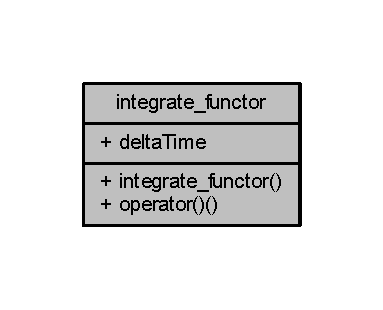
\includegraphics[width=184pt]{structintegrate__functor__coll__graph}
\end{center}
\end{figure}
\subsection*{Metody publiczne}
\begin{DoxyCompactItemize}
\item 
\-\_\-\-\_\-host\-\_\-\-\_\- \-\_\-\-\_\-device\-\_\-\-\_\- \hyperlink{structintegrate__functor_a13075d4c547ba22c37137ff2b874ae45}{integrate\-\_\-functor} (float delta\-\_\-time)
\item 
{\footnotesize template$<$typename Tuple $>$ }\\\-\_\-\-\_\-device\-\_\-\-\_\- void \hyperlink{structintegrate__functor_a772e86ead8690332beb50911e4448f81}{operator()} (Tuple t)
\begin{DoxyCompactList}\small\item\em nowe położenie \end{DoxyCompactList}\end{DoxyCompactItemize}
\subsection*{Atrybuty publiczne}
\begin{DoxyCompactItemize}
\item 
float \hyperlink{structintegrate__functor_a06dce1826719cd5b2a9fdd9f566da754}{delta\-Time}
\end{DoxyCompactItemize}


\subsection{Opis szczegółowy}
ta struktura inicjowana jest z krokiem delta\-\_\-time dla danych opisujących prędkość i położenie cząstki, te dane siedzą w wektorze thrust (w G\-P\-U) jako para (tuple) float4 położenia i prędkości 

Definicja w linii \hyperlink{particles__kernel__impl_8cuh_source_l00046}{46} pliku \hyperlink{particles__kernel__impl_8cuh_source}{particles\-\_\-kernel\-\_\-impl.\-cuh}.



\subsection{Dokumentacja konstruktora i destruktora}
\hypertarget{structintegrate__functor_a13075d4c547ba22c37137ff2b874ae45}{\index{integrate\-\_\-functor@{integrate\-\_\-functor}!integrate\-\_\-functor@{integrate\-\_\-functor}}
\index{integrate\-\_\-functor@{integrate\-\_\-functor}!integrate_functor@{integrate\-\_\-functor}}
\subsubsection[{integrate\-\_\-functor}]{\setlength{\rightskip}{0pt plus 5cm}\-\_\-\-\_\-host\-\_\-\-\_\- \-\_\-\-\_\-device\-\_\-\-\_\- integrate\-\_\-functor\-::integrate\-\_\-functor (
\begin{DoxyParamCaption}
\item[{float}]{delta\-\_\-time}
\end{DoxyParamCaption}
)\hspace{0.3cm}{\ttfamily [inline]}}}\label{structintegrate__functor_a13075d4c547ba22c37137ff2b874ae45}


Definicja w linii \hyperlink{particles__kernel__impl_8cuh_source_l00051}{51} pliku \hyperlink{particles__kernel__impl_8cuh_source}{particles\-\_\-kernel\-\_\-impl.\-cuh}.



Odwołuje się do \hyperlink{particles__kernel__impl_8cuh_source_l00059}{operator()()}.


\begin{DoxyCode}
00051 : \hyperlink{structintegrate__functor_a06dce1826719cd5b2a9fdd9f566da754}{deltaTime}(delta\_time) \{\}
\end{DoxyCode}


Oto graf wywołań dla tej funkcji\-:\nopagebreak
\begin{figure}[H]
\begin{center}
\leavevmode
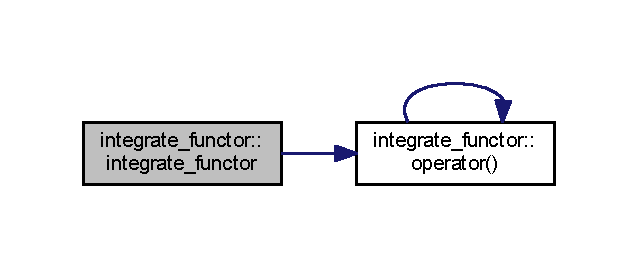
\includegraphics[width=306pt]{structintegrate__functor_a13075d4c547ba22c37137ff2b874ae45_cgraph}
\end{center}
\end{figure}




\subsection{Dokumentacja funkcji składowych}
\hypertarget{structintegrate__functor_a772e86ead8690332beb50911e4448f81}{\index{integrate\-\_\-functor@{integrate\-\_\-functor}!operator()@{operator()}}
\index{operator()@{operator()}!integrate_functor@{integrate\-\_\-functor}}
\subsubsection[{operator()}]{\setlength{\rightskip}{0pt plus 5cm}template$<$typename Tuple $>$ \-\_\-\-\_\-device\-\_\-\-\_\- void integrate\-\_\-functor\-::operator() (
\begin{DoxyParamCaption}
\item[{Tuple}]{t}
\end{DoxyParamCaption}
)\hspace{0.3cm}{\ttfamily [inline]}}}\label{structintegrate__functor_a772e86ead8690332beb50911e4448f81}


nowe położenie 


\begin{DoxyParams}{Parametry}
{\em t} & para położenia i prędkości wylicza nowe położenie i sprawdza czy położenie nie jest za brzegiem \\
\hline
\end{DoxyParams}
$<$ odbijanie sie od kuli 

Definicja w linii \hyperlink{particles__kernel__impl_8cuh_source_l00059}{59} pliku \hyperlink{particles__kernel__impl_8cuh_source}{particles\-\_\-kernel\-\_\-impl.\-cuh}.



Odwołuje się do \hyperlink{particles__kernel__impl_8cuh_source_l00059}{operator()()}.



Odwołania w \hyperlink{particles__kernel__impl_8cuh_source_l00051}{integrate\-\_\-functor()} i \hyperlink{particles__kernel__impl_8cuh_source_l00059}{operator()()}.


\begin{DoxyCode}
00060     \{
00061         \textcolor{keyword}{volatile} float4 posData = thrust::get<0>(t);
00062         \textcolor{keyword}{volatile} float4 velData = thrust::get<1>(t);
00063         float3 pos = make\_float3(posData.x, posData.y, posData.z);
00064         float3 vel = make\_float3(velData.x, velData.y, velData.z);
00065 
00066         vel += \hyperlink{particles__kernel__impl_8cuh_a8db8938e28edd17862daf58651051bdc}{params}.\hyperlink{struct_sim_params_ae7508eba5dd90859215b59d19e001bb9}{gravity} * \hyperlink{structintegrate__functor_a06dce1826719cd5b2a9fdd9f566da754}{deltaTime};
00067         vel *= \hyperlink{particles__kernel__impl_8cuh_a8db8938e28edd17862daf58651051bdc}{params}.\hyperlink{struct_sim_params_a7058bad8c867d9d42d8c9d842638ebea}{globalDamping};
00068 
00069         \textcolor{comment}{// new position = old position + velocity * deltaTime}
00070         pos += vel * \hyperlink{structintegrate__functor_a06dce1826719cd5b2a9fdd9f566da754}{deltaTime};
00071 
00072         \textcolor{comment}{// set this to zero to disable collisions with cube sides}
00073 \textcolor{preprocessor}{#if 0}
00074 \textcolor{preprocessor}{}
00075         \textcolor{keywordflow}{if} (pos.x > 1.0f - \hyperlink{particles__kernel__impl_8cuh_a8db8938e28edd17862daf58651051bdc}{params}.\hyperlink{struct_sim_params_a7e131c24e1020c44173deb0f57a8c4af}{particleRadius})
00076         \{
00077             pos.x = 1.0f - \hyperlink{particles__kernel__impl_8cuh_a8db8938e28edd17862daf58651051bdc}{params}.\hyperlink{struct_sim_params_a7e131c24e1020c44173deb0f57a8c4af}{particleRadius};
00078             vel.x *= \hyperlink{particles__kernel__impl_8cuh_a8db8938e28edd17862daf58651051bdc}{params}.\hyperlink{struct_sim_params_a4da0c7593d6569e48ee50e7d0c7576f9}{boundaryDamping};
00079         \}
00080 
00081         \textcolor{keywordflow}{if} (pos.x < -1.0f + \hyperlink{particles__kernel__impl_8cuh_a8db8938e28edd17862daf58651051bdc}{params}.\hyperlink{struct_sim_params_a7e131c24e1020c44173deb0f57a8c4af}{particleRadius})
00082         \{
00083             pos.x = -1.0f + \hyperlink{particles__kernel__impl_8cuh_a8db8938e28edd17862daf58651051bdc}{params}.\hyperlink{struct_sim_params_a7e131c24e1020c44173deb0f57a8c4af}{particleRadius};
00084             vel.x *= \hyperlink{particles__kernel__impl_8cuh_a8db8938e28edd17862daf58651051bdc}{params}.\hyperlink{struct_sim_params_a4da0c7593d6569e48ee50e7d0c7576f9}{boundaryDamping};
00085         \}
00086 
00087         \textcolor{keywordflow}{if} (pos.y > 1.0f - \hyperlink{particles__kernel__impl_8cuh_a8db8938e28edd17862daf58651051bdc}{params}.\hyperlink{struct_sim_params_a7e131c24e1020c44173deb0f57a8c4af}{particleRadius})
00088         \{
00089             pos.y = 1.0f - \hyperlink{particles__kernel__impl_8cuh_a8db8938e28edd17862daf58651051bdc}{params}.\hyperlink{struct_sim_params_a7e131c24e1020c44173deb0f57a8c4af}{particleRadius};
00090             vel.y *= \hyperlink{particles__kernel__impl_8cuh_a8db8938e28edd17862daf58651051bdc}{params}.\hyperlink{struct_sim_params_a4da0c7593d6569e48ee50e7d0c7576f9}{boundaryDamping};
00091         \}
00092 
00093         \textcolor{keywordflow}{if} (pos.z > 1.0f - \hyperlink{particles__kernel__impl_8cuh_a8db8938e28edd17862daf58651051bdc}{params}.\hyperlink{struct_sim_params_a7e131c24e1020c44173deb0f57a8c4af}{particleRadius})
00094         \{
00095             pos.z = 1.0f - \hyperlink{particles__kernel__impl_8cuh_a8db8938e28edd17862daf58651051bdc}{params}.\hyperlink{struct_sim_params_a7e131c24e1020c44173deb0f57a8c4af}{particleRadius};
00096             vel.z *= \hyperlink{particles__kernel__impl_8cuh_a8db8938e28edd17862daf58651051bdc}{params}.\hyperlink{struct_sim_params_a4da0c7593d6569e48ee50e7d0c7576f9}{boundaryDamping};
00097         \}
00098 
00099         \textcolor{keywordflow}{if} (pos.z < -1.0f + \hyperlink{particles__kernel__impl_8cuh_a8db8938e28edd17862daf58651051bdc}{params}.\hyperlink{struct_sim_params_a7e131c24e1020c44173deb0f57a8c4af}{particleRadius})
00100         \{
00101             pos.z = -1.0f + \hyperlink{particles__kernel__impl_8cuh_a8db8938e28edd17862daf58651051bdc}{params}.\hyperlink{struct_sim_params_a7e131c24e1020c44173deb0f57a8c4af}{particleRadius};
00102             vel.z *= \hyperlink{particles__kernel__impl_8cuh_a8db8938e28edd17862daf58651051bdc}{params}.\hyperlink{struct_sim_params_a4da0c7593d6569e48ee50e7d0c7576f9}{boundaryDamping};
00103         \}
00104 
00105 \textcolor{preprocessor}{#endif}
00106 \textcolor{preprocessor}{}
00108 \textcolor{preprocessor}{#if 1}
00109 \textcolor{preprocessor}{}                \textcolor{keywordtype}{float} xk=pos.x*pos.x;
00110                 \textcolor{keywordtype}{float} yk=pos.y*pos.y;
00111                 \textcolor{keywordtype}{float} zk=pos.z*pos.z;
00112                 \textcolor{keywordtype}{float} r0k=xk+yk+zk;
00113                 \textcolor{keywordtype}{float} r=\hyperlink{particles__kernel__impl_8cuh_a8db8938e28edd17862daf58651051bdc}{params}.\hyperlink{struct_sim_params_af41979948fdd8f76fe28ce2b43eb24cd}{bigradius};\textcolor{comment}{//- params.particleRadius;}
00114                 \textcolor{keywordflow}{if}(r0k > r*r + FLT\_EPSILON )
00115                 \{
00116                         r-=\hyperlink{particles__kernel__impl_8cuh_a8db8938e28edd17862daf58651051bdc}{params}.\hyperlink{struct_sim_params_a7e131c24e1020c44173deb0f57a8c4af}{particleRadius}*4;
00117                         \textcolor{comment}{/*vel.x*=params.boundaryDamping;}
00118 \textcolor{comment}{                        vel.y*=params.boundaryDamping;}
00119 \textcolor{comment}{                        vel.z*=params.boundaryDamping;*/}
00120                         vel.x=0.0f;
00121                         vel.y=0.0f;
00122                         vel.z=0.0f;
00123                         \textcolor{comment}{/*float theta=atan(pos.z/sqrt(pos.x*pos.x+pos.y*pos.y));}
00124 \textcolor{comment}{                        float fi=atan(pos.y/pos.x);}
00125 \textcolor{comment}{                        pos.z=r*sin(theta);}
00126 \textcolor{comment}{                        float rr=r*cos(theta);}
00127 \textcolor{comment}{                        pos.x=rr*cos(fi);}
00128 \textcolor{comment}{                        pos.y=rr*sin(fi);*/}
00129                         \textcolor{keywordtype}{float} r0=sqrt(r0k);
00130                         \textcolor{keywordtype}{float} tmp=r/r0;
00131                         pos.x*=tmp;
00132                         pos.y*=tmp;
00133                         pos.z*=tmp;
00134                 \}
00135 \textcolor{preprocessor}{#endif}
00136 \textcolor{preprocessor}{}
00137 \textcolor{comment}{//dolna plaszczyzna}
00138 \textcolor{preprocessor}{#if 0}
00139 \textcolor{preprocessor}{}        \textcolor{keywordflow}{if} (pos.y < -1.0f + \hyperlink{particles__kernel__impl_8cuh_a8db8938e28edd17862daf58651051bdc}{params}.\hyperlink{struct_sim_params_a7e131c24e1020c44173deb0f57a8c4af}{particleRadius})
00140         \{
00141             pos.y = -1.0f + \hyperlink{particles__kernel__impl_8cuh_a8db8938e28edd17862daf58651051bdc}{params}.\hyperlink{struct_sim_params_a7e131c24e1020c44173deb0f57a8c4af}{particleRadius};
00142             vel.y *= \hyperlink{particles__kernel__impl_8cuh_a8db8938e28edd17862daf58651051bdc}{params}.\hyperlink{struct_sim_params_a4da0c7593d6569e48ee50e7d0c7576f9}{boundaryDamping};
00143         \}
00144 \textcolor{preprocessor}{#endif}
00145 \textcolor{preprocessor}{}
00146         \textcolor{comment}{// store new position and velocity}
00147         thrust::get<0>(t) = make\_float4(pos, posData.w);
00148         thrust::get<1>(t) = make\_float4(vel, velData.w);
00149     \}
\end{DoxyCode}


Oto graf wywołań dla tej funkcji\-:\nopagebreak
\begin{figure}[H]
\begin{center}
\leavevmode
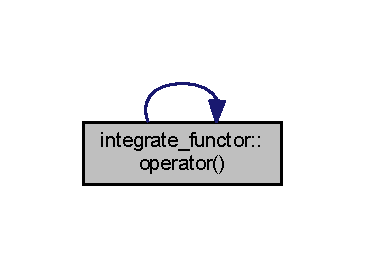
\includegraphics[width=175pt]{structintegrate__functor_a772e86ead8690332beb50911e4448f81_cgraph}
\end{center}
\end{figure}




Oto graf wywoływań tej funkcji\-:\nopagebreak
\begin{figure}[H]
\begin{center}
\leavevmode
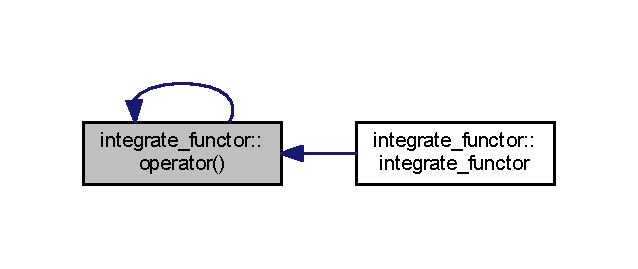
\includegraphics[width=306pt]{structintegrate__functor_a772e86ead8690332beb50911e4448f81_icgraph}
\end{center}
\end{figure}




\subsection{Dokumentacja atrybutów składowych}
\hypertarget{structintegrate__functor_a06dce1826719cd5b2a9fdd9f566da754}{\index{integrate\-\_\-functor@{integrate\-\_\-functor}!delta\-Time@{delta\-Time}}
\index{delta\-Time@{delta\-Time}!integrate_functor@{integrate\-\_\-functor}}
\subsubsection[{delta\-Time}]{\setlength{\rightskip}{0pt plus 5cm}float integrate\-\_\-functor\-::delta\-Time}}\label{structintegrate__functor_a06dce1826719cd5b2a9fdd9f566da754}


Definicja w linii \hyperlink{particles__kernel__impl_8cuh_source_l00048}{48} pliku \hyperlink{particles__kernel__impl_8cuh_source}{particles\-\_\-kernel\-\_\-impl.\-cuh}.



Dokumentacja dla tej struktury została wygenerowana z pliku\-:\begin{DoxyCompactItemize}
\item 
\hyperlink{particles__kernel__impl_8cuh}{particles\-\_\-kernel\-\_\-impl.\-cuh}\end{DoxyCompactItemize}

\hypertarget{class_particle_renderer}{\section{Dokumentacja klasy Particle\-Renderer}
\label{class_particle_renderer}\index{Particle\-Renderer@{Particle\-Renderer}}
}


{\ttfamily \#include $<$render\-\_\-particles.\-h$>$}



Diagram współpracy dla Particle\-Renderer\-:\nopagebreak
\begin{figure}[H]
\begin{center}
\leavevmode
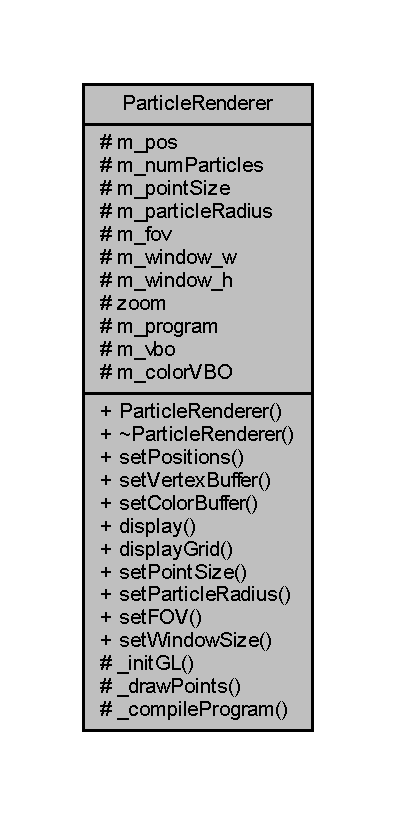
\includegraphics[width=190pt]{class_particle_renderer__coll__graph}
\end{center}
\end{figure}
\subsection*{Typy publiczne}
\begin{DoxyCompactItemize}
\item 
enum \hyperlink{class_particle_renderer_a7b691afffd1abe415cb0ce17fd26f3d5}{Display\-Mode} \{ \hyperlink{class_particle_renderer_a7b691afffd1abe415cb0ce17fd26f3d5a76d84afc3ec5c09bff035fe798dacbbe}{P\-A\-R\-T\-I\-C\-L\-E\-\_\-\-P\-O\-I\-N\-T\-S}, 
\hyperlink{class_particle_renderer_a7b691afffd1abe415cb0ce17fd26f3d5acc641adfb37c1a267e9f91d128094111}{P\-A\-R\-T\-I\-C\-L\-E\-\_\-\-S\-P\-H\-E\-R\-E\-S}, 
\hyperlink{class_particle_renderer_a7b691afffd1abe415cb0ce17fd26f3d5a251fd7044eb27c60bf1eaa1e64a2d2dc}{P\-A\-R\-T\-I\-C\-L\-E\-\_\-\-N\-U\-M\-\_\-\-M\-O\-D\-E\-S}
 \}
\end{DoxyCompactItemize}
\subsection*{Metody publiczne}
\begin{DoxyCompactItemize}
\item 
\hyperlink{class_particle_renderer_a1718484686c2e6db488cc88c433d03cc}{Particle\-Renderer} ()
\item 
\hyperlink{class_particle_renderer_a281be31ad850fead012460fb6675db98}{$\sim$\-Particle\-Renderer} ()
\item 
void \hyperlink{class_particle_renderer_adb3204e8af23a65b05b1aca7f43f0430}{set\-Positions} (float $\ast$pos, int \hyperlink{particles_8cpp_a05b8a90212054a3eb1a036ae0c269596}{num\-Particles})
\item 
void \hyperlink{class_particle_renderer_a9c0d44ba7666ab432004a5df4cbb2b59}{set\-Vertex\-Buffer} (unsigned int vbo, int \hyperlink{particles_8cpp_a05b8a90212054a3eb1a036ae0c269596}{num\-Particles})
\item 
void \hyperlink{class_particle_renderer_af16e23ebcee20753d86d24e4e5e32c7c}{set\-Color\-Buffer} (unsigned int vbo)
\item 
void \hyperlink{class_particle_renderer_a80b2f52dc28bb3abbde021f7fe96f8ff}{display} (\hyperlink{class_particle_renderer_a7b691afffd1abe415cb0ce17fd26f3d5}{Display\-Mode} \hyperlink{particles_8cpp_a1ea5d0cb93f22f7d0fdf804bd68c3326}{mode}=\hyperlink{class_particle_renderer_a7b691afffd1abe415cb0ce17fd26f3d5a76d84afc3ec5c09bff035fe798dacbbe}{P\-A\-R\-T\-I\-C\-L\-E\-\_\-\-P\-O\-I\-N\-T\-S})
\item 
void \hyperlink{class_particle_renderer_a0e0a5d323acf55087911ea77a2a3eafa}{display\-Grid} ()
\item 
void \hyperlink{class_particle_renderer_a68df35cdf53ad987aa6d8360b3531627}{set\-Point\-Size} (float size)
\item 
void \hyperlink{class_particle_renderer_aff09822b565b6953fc83c88bda7fa378}{set\-Particle\-Radius} (float r)
\item 
void \hyperlink{class_particle_renderer_ad6da663d3073401a776edb8dc6cf4d5f}{set\-F\-O\-V} (float fov)
\item 
void \hyperlink{class_particle_renderer_ad84b464475e5ebd42cfed6e2e91e7247}{set\-Window\-Size} (int w, int h)
\end{DoxyCompactItemize}
\subsection*{Metody chronione}
\begin{DoxyCompactItemize}
\item 
void \hyperlink{class_particle_renderer_ac75c7f73a0014333305b174b8863a46b}{\-\_\-init\-G\-L} ()
\item 
void \hyperlink{class_particle_renderer_a2683c43c010bff7973a977c1953f2bd6}{\-\_\-draw\-Points} ()
\item 
G\-Luint \hyperlink{class_particle_renderer_a3a7af352d38734b6bfa425e3b207d60b}{\-\_\-compile\-Program} (const char $\ast$vsource, const char $\ast$fsource)
\end{DoxyCompactItemize}
\subsection*{Atrybuty chronione}
\begin{DoxyCompactItemize}
\item 
float $\ast$ \hyperlink{class_particle_renderer_a1d74720edb5c3a13edcdd176ac0d84c7}{m\-\_\-pos}
\item 
int \hyperlink{class_particle_renderer_af885fdb5e6da925209dfd960f66b5fd8}{m\-\_\-num\-Particles}
\item 
float \hyperlink{class_particle_renderer_a1ca13e546c937cb546c0da19fa853b34}{m\-\_\-point\-Size}
\item 
float \hyperlink{class_particle_renderer_aab5ee3cd769a64c45dc9714aabdb0ee2}{m\-\_\-particle\-Radius}
\item 
float \hyperlink{class_particle_renderer_a0aed003bd557a3c32ca7d2ca89fc59f7}{m\-\_\-fov}
\item 
int \hyperlink{class_particle_renderer_aa71b7eba5d5665a086b7ba80adddf19b}{m\-\_\-window\-\_\-w}
\item 
int \hyperlink{class_particle_renderer_af34b1e93f6a7f22774a6473c52027d77}{m\-\_\-window\-\_\-h}
\item 
G\-Luint \hyperlink{class_particle_renderer_ab8f0dd1a6e0f4401012bd46ae8940648}{m\-\_\-program}
\item 
G\-Luint \hyperlink{class_particle_renderer_a7549feaa0982abbc44c9fe73f2eb251f}{m\-\_\-vbo}
\item 
G\-Luint \hyperlink{class_particle_renderer_a7dcaa73a41c598207974432206b423b5}{m\-\_\-color\-V\-B\-O}
\end{DoxyCompactItemize}


\subsection{Opis szczegółowy}


Definicja w linii \hyperlink{render__particles_8h_source_l00015}{15} pliku \hyperlink{render__particles_8h_source}{render\-\_\-particles.\-h}.



\subsection{Dokumentacja składowych wyliczanych}
\hypertarget{class_particle_renderer_a7b691afffd1abe415cb0ce17fd26f3d5}{\index{Particle\-Renderer@{Particle\-Renderer}!Display\-Mode@{Display\-Mode}}
\index{Display\-Mode@{Display\-Mode}!ParticleRenderer@{Particle\-Renderer}}
\subsubsection[{Display\-Mode}]{\setlength{\rightskip}{0pt plus 5cm}enum {\bf Particle\-Renderer\-::\-Display\-Mode}}}\label{class_particle_renderer_a7b691afffd1abe415cb0ce17fd26f3d5}
\begin{Desc}
\item[Wartości wyliczeń]\par
\begin{description}
\index{P\-A\-R\-T\-I\-C\-L\-E\-\_\-\-P\-O\-I\-N\-T\-S@{P\-A\-R\-T\-I\-C\-L\-E\-\_\-\-P\-O\-I\-N\-T\-S}!Particle\-Renderer@{Particle\-Renderer}}\index{Particle\-Renderer@{Particle\-Renderer}!P\-A\-R\-T\-I\-C\-L\-E\-\_\-\-P\-O\-I\-N\-T\-S@{P\-A\-R\-T\-I\-C\-L\-E\-\_\-\-P\-O\-I\-N\-T\-S}}\item[{\em 
\hypertarget{class_particle_renderer_a7b691afffd1abe415cb0ce17fd26f3d5a76d84afc3ec5c09bff035fe798dacbbe}{P\-A\-R\-T\-I\-C\-L\-E\-\_\-\-P\-O\-I\-N\-T\-S}\label{class_particle_renderer_a7b691afffd1abe415cb0ce17fd26f3d5a76d84afc3ec5c09bff035fe798dacbbe}
}]\index{P\-A\-R\-T\-I\-C\-L\-E\-\_\-\-S\-P\-H\-E\-R\-E\-S@{P\-A\-R\-T\-I\-C\-L\-E\-\_\-\-S\-P\-H\-E\-R\-E\-S}!Particle\-Renderer@{Particle\-Renderer}}\index{Particle\-Renderer@{Particle\-Renderer}!P\-A\-R\-T\-I\-C\-L\-E\-\_\-\-S\-P\-H\-E\-R\-E\-S@{P\-A\-R\-T\-I\-C\-L\-E\-\_\-\-S\-P\-H\-E\-R\-E\-S}}\item[{\em 
\hypertarget{class_particle_renderer_a7b691afffd1abe415cb0ce17fd26f3d5acc641adfb37c1a267e9f91d128094111}{P\-A\-R\-T\-I\-C\-L\-E\-\_\-\-S\-P\-H\-E\-R\-E\-S}\label{class_particle_renderer_a7b691afffd1abe415cb0ce17fd26f3d5acc641adfb37c1a267e9f91d128094111}
}]\index{P\-A\-R\-T\-I\-C\-L\-E\-\_\-\-N\-U\-M\-\_\-\-M\-O\-D\-E\-S@{P\-A\-R\-T\-I\-C\-L\-E\-\_\-\-N\-U\-M\-\_\-\-M\-O\-D\-E\-S}!Particle\-Renderer@{Particle\-Renderer}}\index{Particle\-Renderer@{Particle\-Renderer}!P\-A\-R\-T\-I\-C\-L\-E\-\_\-\-N\-U\-M\-\_\-\-M\-O\-D\-E\-S@{P\-A\-R\-T\-I\-C\-L\-E\-\_\-\-N\-U\-M\-\_\-\-M\-O\-D\-E\-S}}\item[{\em 
\hypertarget{class_particle_renderer_a7b691afffd1abe415cb0ce17fd26f3d5a251fd7044eb27c60bf1eaa1e64a2d2dc}{P\-A\-R\-T\-I\-C\-L\-E\-\_\-\-N\-U\-M\-\_\-\-M\-O\-D\-E\-S}\label{class_particle_renderer_a7b691afffd1abe415cb0ce17fd26f3d5a251fd7044eb27c60bf1eaa1e64a2d2dc}
}]\end{description}
\end{Desc}


Definicja w linii \hyperlink{render__particles_8h_source_l00028}{28} pliku \hyperlink{render__particles_8h_source}{render\-\_\-particles.\-h}.


\begin{DoxyCode}
00029         \{
00030             \hyperlink{class_particle_renderer_a7b691afffd1abe415cb0ce17fd26f3d5a76d84afc3ec5c09bff035fe798dacbbe}{PARTICLE\_POINTS},
00031             \hyperlink{class_particle_renderer_a7b691afffd1abe415cb0ce17fd26f3d5acc641adfb37c1a267e9f91d128094111}{PARTICLE\_SPHERES},
00032             \hyperlink{class_particle_renderer_a7b691afffd1abe415cb0ce17fd26f3d5a251fd7044eb27c60bf1eaa1e64a2d2dc}{PARTICLE\_NUM\_MODES}
00033         \};
\end{DoxyCode}


\subsection{Dokumentacja konstruktora i destruktora}
\hypertarget{class_particle_renderer_a1718484686c2e6db488cc88c433d03cc}{\index{Particle\-Renderer@{Particle\-Renderer}!Particle\-Renderer@{Particle\-Renderer}}
\index{Particle\-Renderer@{Particle\-Renderer}!ParticleRenderer@{Particle\-Renderer}}
\subsubsection[{Particle\-Renderer}]{\setlength{\rightskip}{0pt plus 5cm}Particle\-Renderer\-::\-Particle\-Renderer (
\begin{DoxyParamCaption}
{}
\end{DoxyParamCaption}
)}}\label{class_particle_renderer_a1718484686c2e6db488cc88c433d03cc}


Definicja w linii \hyperlink{render__particles_8cpp_source_l00025}{25} pliku \hyperlink{render__particles_8cpp_source}{render\-\_\-particles.\-cpp}.



Odwołuje się do \hyperlink{render__particles_8cpp_source_l00157}{\-\_\-init\-G\-L()}, \hyperlink{render__particles_8h_source_l00063}{m\-\_\-num\-Particles}, \hyperlink{render__particles_8h_source_l00066}{m\-\_\-particle\-Radius}, \hyperlink{render__particles_8h_source_l00065}{m\-\_\-point\-Size}, \hyperlink{render__particles_8h_source_l00062}{m\-\_\-pos} i \hyperlink{render__particles_8cpp_source_l00025}{Particle\-Renderer()}.



Odwołania w \hyperlink{render__particles_8cpp_source_l00025}{Particle\-Renderer()}.


\begin{DoxyCode}
00026     : \hyperlink{class_particle_renderer_a1d74720edb5c3a13edcdd176ac0d84c7}{m\_pos}(0),
00027       \hyperlink{class_particle_renderer_af885fdb5e6da925209dfd960f66b5fd8}{m\_numParticles}(0),
00028       \hyperlink{class_particle_renderer_a1ca13e546c937cb546c0da19fa853b34}{m\_pointSize}(1.0f),
00029       \hyperlink{class_particle_renderer_aab5ee3cd769a64c45dc9714aabdb0ee2}{m\_particleRadius}(0.125f * 0.5f),
00030       \hyperlink{class_particle_renderer_ab8f0dd1a6e0f4401012bd46ae8940648}{m\_program}(0),
00031       \hyperlink{class_particle_renderer_a7549feaa0982abbc44c9fe73f2eb251f}{m\_vbo}(0),
00032       \hyperlink{class_particle_renderer_a7dcaa73a41c598207974432206b423b5}{m\_colorVBO}(0)
00033 \{
00034     \hyperlink{class_particle_renderer_ac75c7f73a0014333305b174b8863a46b}{\_initGL}();
00035 \}
\end{DoxyCode}


Oto graf wywołań dla tej funkcji\-:\nopagebreak
\begin{figure}[H]
\begin{center}
\leavevmode
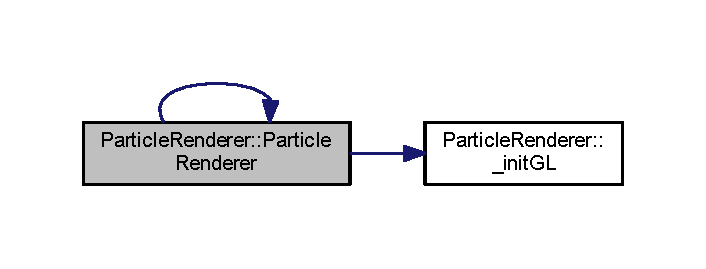
\includegraphics[width=339pt]{class_particle_renderer_a1718484686c2e6db488cc88c433d03cc_cgraph}
\end{center}
\end{figure}




Oto graf wywoływań tej funkcji\-:\nopagebreak
\begin{figure}[H]
\begin{center}
\leavevmode
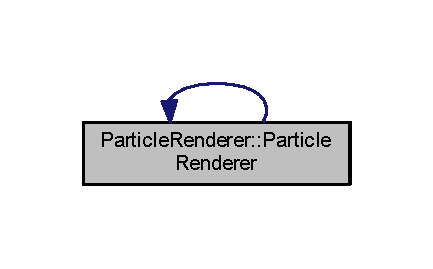
\includegraphics[width=208pt]{class_particle_renderer_a1718484686c2e6db488cc88c433d03cc_icgraph}
\end{center}
\end{figure}


\hypertarget{class_particle_renderer_a281be31ad850fead012460fb6675db98}{\index{Particle\-Renderer@{Particle\-Renderer}!$\sim$\-Particle\-Renderer@{$\sim$\-Particle\-Renderer}}
\index{$\sim$\-Particle\-Renderer@{$\sim$\-Particle\-Renderer}!ParticleRenderer@{Particle\-Renderer}}
\subsubsection[{$\sim$\-Particle\-Renderer}]{\setlength{\rightskip}{0pt plus 5cm}Particle\-Renderer\-::$\sim$\-Particle\-Renderer (
\begin{DoxyParamCaption}
{}
\end{DoxyParamCaption}
)}}\label{class_particle_renderer_a281be31ad850fead012460fb6675db98}


Definicja w linii \hyperlink{render__particles_8cpp_source_l00037}{37} pliku \hyperlink{render__particles_8cpp_source}{render\-\_\-particles.\-cpp}.



Odwołuje się do \hyperlink{render__particles_8h_source_l00062}{m\-\_\-pos}.


\begin{DoxyCode}
00038 \{
00039     \hyperlink{class_particle_renderer_a1d74720edb5c3a13edcdd176ac0d84c7}{m\_pos} = 0;
00040 \}
\end{DoxyCode}


\subsection{Dokumentacja funkcji składowych}
\hypertarget{class_particle_renderer_a3a7af352d38734b6bfa425e3b207d60b}{\index{Particle\-Renderer@{Particle\-Renderer}!\-\_\-compile\-Program@{\-\_\-compile\-Program}}
\index{\-\_\-compile\-Program@{\-\_\-compile\-Program}!ParticleRenderer@{Particle\-Renderer}}
\subsubsection[{\-\_\-compile\-Program}]{\setlength{\rightskip}{0pt plus 5cm}G\-Luint Particle\-Renderer\-::\-\_\-compile\-Program (
\begin{DoxyParamCaption}
\item[{const char $\ast$}]{vsource, }
\item[{const char $\ast$}]{fsource}
\end{DoxyParamCaption}
)\hspace{0.3cm}{\ttfamily [protected]}}}\label{class_particle_renderer_a3a7af352d38734b6bfa425e3b207d60b}


Definicja w linii \hyperlink{render__particles_8cpp_source_l00123}{123} pliku \hyperlink{render__particles_8cpp_source}{render\-\_\-particles.\-cpp}.


\begin{DoxyCode}
00124 \{
00125     GLuint \hyperlink{shaders_8h_aea8e0959f6b7eabf6156f801e179da60}{vertexShader} = glCreateShader(GL\_VERTEX\_SHADER);
00126     GLuint fragmentShader = glCreateShader(GL\_FRAGMENT\_SHADER);
00127 
00128     glShaderSource(vertexShader, 1, &vsource, 0);
00129     glShaderSource(fragmentShader, 1, &fsource, 0);
00130 
00131     glCompileShader(vertexShader);
00132     glCompileShader(fragmentShader);
00133 
00134     GLuint program = glCreateProgram();
00135 
00136     glAttachShader(program, vertexShader);
00137     glAttachShader(program, fragmentShader);
00138 
00139     glLinkProgram(program);
00140 
00141     \textcolor{comment}{// check if program linked}
00142     GLint success = 0;
00143     glGetProgramiv(program, GL\_LINK\_STATUS, &success);
00144 
00145     \textcolor{keywordflow}{if} (!success)
00146     \{
00147         \textcolor{keywordtype}{char} temp[256];
00148         glGetProgramInfoLog(program, 256, 0, temp);
00149         printf(\textcolor{stringliteral}{"Failed to link program:\(\backslash\)n%s\(\backslash\)n"}, temp);
00150         glDeleteProgram(program);
00151         program = 0;
00152     \}
00153 
00154     \textcolor{keywordflow}{return} program;
00155 \}
\end{DoxyCode}
\hypertarget{class_particle_renderer_a2683c43c010bff7973a977c1953f2bd6}{\index{Particle\-Renderer@{Particle\-Renderer}!\-\_\-draw\-Points@{\-\_\-draw\-Points}}
\index{\-\_\-draw\-Points@{\-\_\-draw\-Points}!ParticleRenderer@{Particle\-Renderer}}
\subsubsection[{\-\_\-draw\-Points}]{\setlength{\rightskip}{0pt plus 5cm}void Particle\-Renderer\-::\-\_\-draw\-Points (
\begin{DoxyParamCaption}
{}
\end{DoxyParamCaption}
)\hspace{0.3cm}{\ttfamily [protected]}}}\label{class_particle_renderer_a2683c43c010bff7973a977c1953f2bd6}


Definicja w linii \hyperlink{render__particles_8cpp_source_l00054}{54} pliku \hyperlink{render__particles_8cpp_source}{render\-\_\-particles.\-cpp}.



Odwołania w \hyperlink{render__particles_8cpp_source_l00091}{display()}.


\begin{DoxyCode}
00055 \{
00056     \textcolor{keywordflow}{if} (!\hyperlink{class_particle_renderer_a7549feaa0982abbc44c9fe73f2eb251f}{m\_vbo})
00057     \{
00058         glBegin(GL\_POINTS);
00059         \{
00060             \textcolor{keywordtype}{int} k = 0;
00061 
00062             \textcolor{keywordflow}{for} (\textcolor{keywordtype}{int} i = 0; i < \hyperlink{class_particle_renderer_af885fdb5e6da925209dfd960f66b5fd8}{m\_numParticles}; ++i)
00063             \{
00064                 glVertex3fv(&\hyperlink{class_particle_renderer_a1d74720edb5c3a13edcdd176ac0d84c7}{m\_pos}[k]);
00065                 k += 4;
00066             \}
00067         \}
00068         glEnd();
00069     \}
00070     \textcolor{keywordflow}{else}
00071     \{
00072         glBindBufferARB(GL\_ARRAY\_BUFFER\_ARB, \hyperlink{class_particle_renderer_a7549feaa0982abbc44c9fe73f2eb251f}{m\_vbo});
00073         glVertexPointer(4, GL\_FLOAT, 0, 0);
00074         glEnableClientState(GL\_VERTEX\_ARRAY);
00075 
00076         \textcolor{keywordflow}{if} (\hyperlink{class_particle_renderer_a7dcaa73a41c598207974432206b423b5}{m\_colorVBO})
00077         \{
00078             glBindBufferARB(GL\_ARRAY\_BUFFER\_ARB, \hyperlink{class_particle_renderer_a7dcaa73a41c598207974432206b423b5}{m\_colorVBO});
00079             glColorPointer(4, GL\_FLOAT, 0, 0);
00080             glEnableClientState(GL\_COLOR\_ARRAY);
00081         \}
00082 
00083         glDrawArrays(GL\_POINTS, 0, \hyperlink{class_particle_renderer_af885fdb5e6da925209dfd960f66b5fd8}{m\_numParticles});
00084 
00085         glBindBufferARB(GL\_ARRAY\_BUFFER\_ARB, 0);
00086         glDisableClientState(GL\_VERTEX\_ARRAY);
00087         glDisableClientState(GL\_COLOR\_ARRAY);
00088     \}
00089 \}
\end{DoxyCode}


Oto graf wywoływań tej funkcji\-:\nopagebreak
\begin{figure}[H]
\begin{center}
\leavevmode
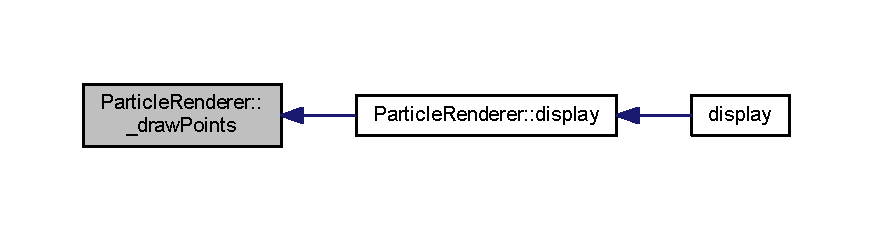
\includegraphics[width=350pt]{class_particle_renderer_a2683c43c010bff7973a977c1953f2bd6_icgraph}
\end{center}
\end{figure}


\hypertarget{class_particle_renderer_ac75c7f73a0014333305b174b8863a46b}{\index{Particle\-Renderer@{Particle\-Renderer}!\-\_\-init\-G\-L@{\-\_\-init\-G\-L}}
\index{\-\_\-init\-G\-L@{\-\_\-init\-G\-L}!ParticleRenderer@{Particle\-Renderer}}
\subsubsection[{\-\_\-init\-G\-L}]{\setlength{\rightskip}{0pt plus 5cm}void Particle\-Renderer\-::\-\_\-init\-G\-L (
\begin{DoxyParamCaption}
{}
\end{DoxyParamCaption}
)\hspace{0.3cm}{\ttfamily [protected]}}}\label{class_particle_renderer_ac75c7f73a0014333305b174b8863a46b}


Definicja w linii \hyperlink{render__particles_8cpp_source_l00157}{157} pliku \hyperlink{render__particles_8cpp_source}{render\-\_\-particles.\-cpp}.



Odwołania w \hyperlink{render__particles_8cpp_source_l00025}{Particle\-Renderer()}.


\begin{DoxyCode}
00158 \{
00159     \hyperlink{class_particle_renderer_ab8f0dd1a6e0f4401012bd46ae8940648}{m\_program} = \hyperlink{class_particle_renderer_a3a7af352d38734b6bfa425e3b207d60b}{\_compileProgram}(\hyperlink{shaders_8h_aea8e0959f6b7eabf6156f801e179da60}{vertexShader}, 
      \hyperlink{shaders_8h_abad1d2b70401d6f3a4f61a462369373d}{spherePixelShader});
00160 
00161 \textcolor{preprocessor}{#if !defined(\_\_APPLE\_\_) && !defined(MACOSX)}
00162 \textcolor{preprocessor}{}    glClampColorARB(GL\_CLAMP\_VERTEX\_COLOR\_ARB, GL\_FALSE);
00163     glClampColorARB(GL\_CLAMP\_FRAGMENT\_COLOR\_ARB, GL\_FALSE);
00164 \textcolor{preprocessor}{#endif}
00165 \textcolor{preprocessor}{}\}
\end{DoxyCode}


Oto graf wywoływań tej funkcji\-:\nopagebreak
\begin{figure}[H]
\begin{center}
\leavevmode
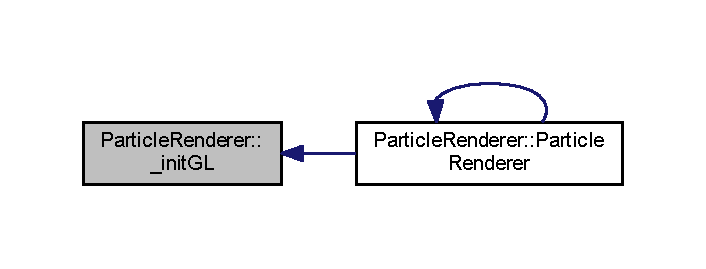
\includegraphics[width=339pt]{class_particle_renderer_ac75c7f73a0014333305b174b8863a46b_icgraph}
\end{center}
\end{figure}


\hypertarget{class_particle_renderer_a80b2f52dc28bb3abbde021f7fe96f8ff}{\index{Particle\-Renderer@{Particle\-Renderer}!display@{display}}
\index{display@{display}!ParticleRenderer@{Particle\-Renderer}}
\subsubsection[{display}]{\setlength{\rightskip}{0pt plus 5cm}void Particle\-Renderer\-::display (
\begin{DoxyParamCaption}
\item[{{\bf Display\-Mode}}]{mode = {\ttfamily {\bf P\-A\-R\-T\-I\-C\-L\-E\-\_\-\-P\-O\-I\-N\-T\-S}}}
\end{DoxyParamCaption}
)}}\label{class_particle_renderer_a80b2f52dc28bb3abbde021f7fe96f8ff}


Definicja w linii \hyperlink{render__particles_8cpp_source_l00091}{91} pliku \hyperlink{render__particles_8cpp_source}{render\-\_\-particles.\-cpp}.



Odwołuje się do \hyperlink{render__particles_8cpp_source_l00054}{\-\_\-draw\-Points()}.



Odwołania w \hyperlink{particles_8cpp_source_l00248}{display()}.


\begin{DoxyCode}
00092 \{
00093     \textcolor{keywordflow}{switch} (\hyperlink{particles_8cpp_a1ea5d0cb93f22f7d0fdf804bd68c3326}{mode})
00094     \{
00095         \textcolor{keywordflow}{case} \hyperlink{class_particle_renderer_a7b691afffd1abe415cb0ce17fd26f3d5a76d84afc3ec5c09bff035fe798dacbbe}{PARTICLE\_POINTS}:
00096             glColor3f(1, 1, 1);
00097             glPointSize(\hyperlink{class_particle_renderer_a1ca13e546c937cb546c0da19fa853b34}{m\_pointSize});
00098             \hyperlink{class_particle_renderer_a2683c43c010bff7973a977c1953f2bd6}{\_drawPoints}();
00099             \textcolor{keywordflow}{break};
00100 
00101         \textcolor{keywordflow}{default}:
00102         \textcolor{keywordflow}{case} \hyperlink{class_particle_renderer_a7b691afffd1abe415cb0ce17fd26f3d5acc641adfb37c1a267e9f91d128094111}{PARTICLE\_SPHERES}:
00103             glEnable(GL\_POINT\_SPRITE\_ARB);
00104             glTexEnvi(GL\_POINT\_SPRITE\_ARB, GL\_COORD\_REPLACE\_ARB, GL\_TRUE);
00105             glEnable(GL\_VERTEX\_PROGRAM\_POINT\_SIZE\_NV);
00106             glDepthMask(GL\_TRUE);
00107             glEnable(GL\_DEPTH\_TEST);
00108 
00109             glUseProgram(\hyperlink{class_particle_renderer_ab8f0dd1a6e0f4401012bd46ae8940648}{m\_program});
00110             glUniform1f(glGetUniformLocation(\hyperlink{class_particle_renderer_ab8f0dd1a6e0f4401012bd46ae8940648}{m\_program}, \textcolor{stringliteral}{"pointScale"}), 
      \hyperlink{class_particle_renderer_af34b1e93f6a7f22774a6473c52027d77}{m\_window\_h} / tanf(\hyperlink{class_particle_renderer_a0aed003bd557a3c32ca7d2ca89fc59f7}{m\_fov}*0.5f*(\textcolor{keywordtype}{float})\hyperlink{render__particles_8cpp_ae71449b1cc6e6250b91f539153a7a0d3}{M\_PI}/180.0f));
00111             glUniform1f(glGetUniformLocation(\hyperlink{class_particle_renderer_ab8f0dd1a6e0f4401012bd46ae8940648}{m\_program}, \textcolor{stringliteral}{"pointRadius"}), 
      \hyperlink{class_particle_renderer_aab5ee3cd769a64c45dc9714aabdb0ee2}{m\_particleRadius});
00112 
00113             glColor3f(1, 1, 1);
00114             \hyperlink{class_particle_renderer_a2683c43c010bff7973a977c1953f2bd6}{\_drawPoints}();
00115 
00116             glUseProgram(0);
00117             glDisable(GL\_POINT\_SPRITE\_ARB);
00118             \textcolor{keywordflow}{break};
00119     \}
00120 \}
\end{DoxyCode}


Oto graf wywołań dla tej funkcji\-:\nopagebreak
\begin{figure}[H]
\begin{center}
\leavevmode
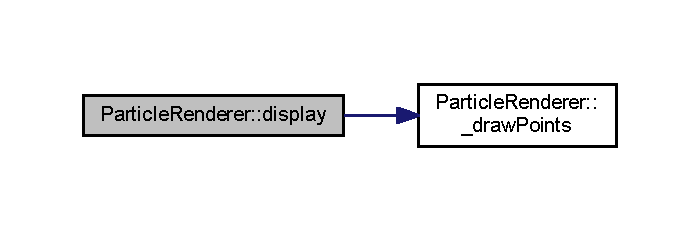
\includegraphics[width=336pt]{class_particle_renderer_a80b2f52dc28bb3abbde021f7fe96f8ff_cgraph}
\end{center}
\end{figure}




Oto graf wywoływań tej funkcji\-:\nopagebreak
\begin{figure}[H]
\begin{center}
\leavevmode
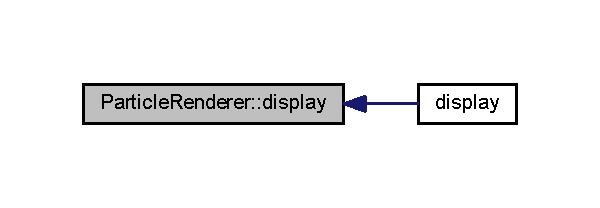
\includegraphics[width=288pt]{class_particle_renderer_a80b2f52dc28bb3abbde021f7fe96f8ff_icgraph}
\end{center}
\end{figure}


\hypertarget{class_particle_renderer_a0e0a5d323acf55087911ea77a2a3eafa}{\index{Particle\-Renderer@{Particle\-Renderer}!display\-Grid@{display\-Grid}}
\index{display\-Grid@{display\-Grid}!ParticleRenderer@{Particle\-Renderer}}
\subsubsection[{display\-Grid}]{\setlength{\rightskip}{0pt plus 5cm}void Particle\-Renderer\-::display\-Grid (
\begin{DoxyParamCaption}
{}
\end{DoxyParamCaption}
)}}\label{class_particle_renderer_a0e0a5d323acf55087911ea77a2a3eafa}
\hypertarget{class_particle_renderer_af16e23ebcee20753d86d24e4e5e32c7c}{\index{Particle\-Renderer@{Particle\-Renderer}!set\-Color\-Buffer@{set\-Color\-Buffer}}
\index{set\-Color\-Buffer@{set\-Color\-Buffer}!ParticleRenderer@{Particle\-Renderer}}
\subsubsection[{set\-Color\-Buffer}]{\setlength{\rightskip}{0pt plus 5cm}void Particle\-Renderer\-::set\-Color\-Buffer (
\begin{DoxyParamCaption}
\item[{unsigned int}]{vbo}
\end{DoxyParamCaption}
)\hspace{0.3cm}{\ttfamily [inline]}}}\label{class_particle_renderer_af16e23ebcee20753d86d24e4e5e32c7c}


Definicja w linii \hyperlink{render__particles_8h_source_l00023}{23} pliku \hyperlink{render__particles_8h_source}{render\-\_\-particles.\-h}.



Odwołania w \hyperlink{particles_8cpp_source_l00142}{init\-Particle\-System()}.


\begin{DoxyCode}
00024         \{
00025             \hyperlink{class_particle_renderer_a7dcaa73a41c598207974432206b423b5}{m\_colorVBO} = vbo;
00026         \}
\end{DoxyCode}


Oto graf wywoływań tej funkcji\-:\nopagebreak
\begin{figure}[H]
\begin{center}
\leavevmode
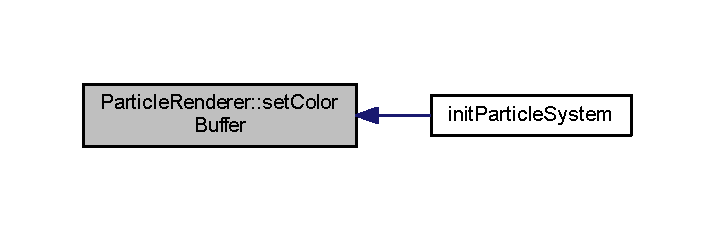
\includegraphics[width=343pt]{class_particle_renderer_af16e23ebcee20753d86d24e4e5e32c7c_icgraph}
\end{center}
\end{figure}


\hypertarget{class_particle_renderer_ad6da663d3073401a776edb8dc6cf4d5f}{\index{Particle\-Renderer@{Particle\-Renderer}!set\-F\-O\-V@{set\-F\-O\-V}}
\index{set\-F\-O\-V@{set\-F\-O\-V}!ParticleRenderer@{Particle\-Renderer}}
\subsubsection[{set\-F\-O\-V}]{\setlength{\rightskip}{0pt plus 5cm}void Particle\-Renderer\-::set\-F\-O\-V (
\begin{DoxyParamCaption}
\item[{float}]{fov}
\end{DoxyParamCaption}
)\hspace{0.3cm}{\ttfamily [inline]}}}\label{class_particle_renderer_ad6da663d3073401a776edb8dc6cf4d5f}


Definicja w linii \hyperlink{render__particles_8h_source_l00046}{46} pliku \hyperlink{render__particles_8h_source}{render\-\_\-particles.\-h}.



Odwołuje się do \hyperlink{render__particles_8h_source_l00067}{m\-\_\-fov}.



Odwołania w \hyperlink{particles_8cpp_source_l00353}{reshape()}.


\begin{DoxyCode}
00047         \{
00048             \hyperlink{class_particle_renderer_a0aed003bd557a3c32ca7d2ca89fc59f7}{m\_fov} = fov;
00049         \}
\end{DoxyCode}


Oto graf wywoływań tej funkcji\-:\nopagebreak
\begin{figure}[H]
\begin{center}
\leavevmode
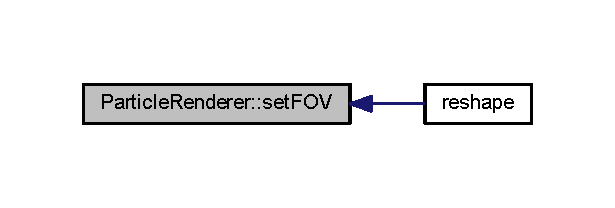
\includegraphics[width=295pt]{class_particle_renderer_ad6da663d3073401a776edb8dc6cf4d5f_icgraph}
\end{center}
\end{figure}


\hypertarget{class_particle_renderer_aff09822b565b6953fc83c88bda7fa378}{\index{Particle\-Renderer@{Particle\-Renderer}!set\-Particle\-Radius@{set\-Particle\-Radius}}
\index{set\-Particle\-Radius@{set\-Particle\-Radius}!ParticleRenderer@{Particle\-Renderer}}
\subsubsection[{set\-Particle\-Radius}]{\setlength{\rightskip}{0pt plus 5cm}void Particle\-Renderer\-::set\-Particle\-Radius (
\begin{DoxyParamCaption}
\item[{float}]{r}
\end{DoxyParamCaption}
)\hspace{0.3cm}{\ttfamily [inline]}}}\label{class_particle_renderer_aff09822b565b6953fc83c88bda7fa378}


Definicja w linii \hyperlink{render__particles_8h_source_l00042}{42} pliku \hyperlink{render__particles_8h_source}{render\-\_\-particles.\-h}.



Odwołuje się do \hyperlink{render__particles_8h_source_l00066}{m\-\_\-particle\-Radius}.



Odwołania w \hyperlink{particles_8cpp_source_l00142}{init\-Particle\-System()}.


\begin{DoxyCode}
00043         \{
00044             \hyperlink{class_particle_renderer_aab5ee3cd769a64c45dc9714aabdb0ee2}{m\_particleRadius} = r;
00045         \}
\end{DoxyCode}


Oto graf wywoływań tej funkcji\-:\nopagebreak
\begin{figure}[H]
\begin{center}
\leavevmode
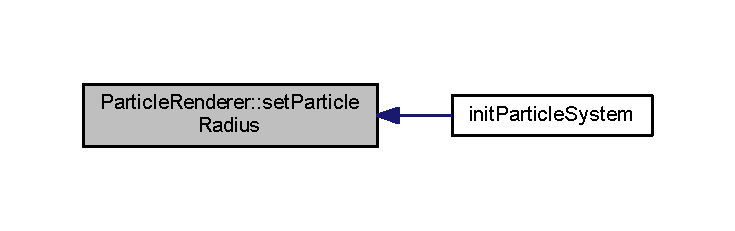
\includegraphics[width=350pt]{class_particle_renderer_aff09822b565b6953fc83c88bda7fa378_icgraph}
\end{center}
\end{figure}


\hypertarget{class_particle_renderer_a68df35cdf53ad987aa6d8360b3531627}{\index{Particle\-Renderer@{Particle\-Renderer}!set\-Point\-Size@{set\-Point\-Size}}
\index{set\-Point\-Size@{set\-Point\-Size}!ParticleRenderer@{Particle\-Renderer}}
\subsubsection[{set\-Point\-Size}]{\setlength{\rightskip}{0pt plus 5cm}void Particle\-Renderer\-::set\-Point\-Size (
\begin{DoxyParamCaption}
\item[{float}]{size}
\end{DoxyParamCaption}
)\hspace{0.3cm}{\ttfamily [inline]}}}\label{class_particle_renderer_a68df35cdf53ad987aa6d8360b3531627}


Definicja w linii \hyperlink{render__particles_8h_source_l00038}{38} pliku \hyperlink{render__particles_8h_source}{render\-\_\-particles.\-h}.



Odwołuje się do \hyperlink{render__particles_8h_source_l00065}{m\-\_\-point\-Size}.


\begin{DoxyCode}
00039         \{
00040             \hyperlink{class_particle_renderer_a1ca13e546c937cb546c0da19fa853b34}{m\_pointSize} = size;
00041         \}
\end{DoxyCode}
\hypertarget{class_particle_renderer_adb3204e8af23a65b05b1aca7f43f0430}{\index{Particle\-Renderer@{Particle\-Renderer}!set\-Positions@{set\-Positions}}
\index{set\-Positions@{set\-Positions}!ParticleRenderer@{Particle\-Renderer}}
\subsubsection[{set\-Positions}]{\setlength{\rightskip}{0pt plus 5cm}void Particle\-Renderer\-::set\-Positions (
\begin{DoxyParamCaption}
\item[{float $\ast$}]{pos, }
\item[{int}]{num\-Particles}
\end{DoxyParamCaption}
)}}\label{class_particle_renderer_adb3204e8af23a65b05b1aca7f43f0430}


Definicja w linii \hyperlink{render__particles_8cpp_source_l00042}{42} pliku \hyperlink{render__particles_8cpp_source}{render\-\_\-particles.\-cpp}.



Odwołuje się do \hyperlink{render__particles_8h_source_l00063}{m\-\_\-num\-Particles} i \hyperlink{render__particles_8h_source_l00062}{m\-\_\-pos}.


\begin{DoxyCode}
00043 \{
00044     \hyperlink{class_particle_renderer_a1d74720edb5c3a13edcdd176ac0d84c7}{m\_pos} = pos;
00045     \hyperlink{class_particle_renderer_af885fdb5e6da925209dfd960f66b5fd8}{m\_numParticles} = \hyperlink{particles_8cpp_a05b8a90212054a3eb1a036ae0c269596}{numParticles};
00046 \}
\end{DoxyCode}
\hypertarget{class_particle_renderer_a9c0d44ba7666ab432004a5df4cbb2b59}{\index{Particle\-Renderer@{Particle\-Renderer}!set\-Vertex\-Buffer@{set\-Vertex\-Buffer}}
\index{set\-Vertex\-Buffer@{set\-Vertex\-Buffer}!ParticleRenderer@{Particle\-Renderer}}
\subsubsection[{set\-Vertex\-Buffer}]{\setlength{\rightskip}{0pt plus 5cm}void Particle\-Renderer\-::set\-Vertex\-Buffer (
\begin{DoxyParamCaption}
\item[{unsigned int}]{vbo, }
\item[{int}]{num\-Particles}
\end{DoxyParamCaption}
)}}\label{class_particle_renderer_a9c0d44ba7666ab432004a5df4cbb2b59}


Definicja w linii \hyperlink{render__particles_8cpp_source_l00048}{48} pliku \hyperlink{render__particles_8cpp_source}{render\-\_\-particles.\-cpp}.



Odwołuje się do \hyperlink{render__particles_8h_source_l00063}{m\-\_\-num\-Particles}.



Odwołania w \hyperlink{particles_8cpp_source_l00248}{display()} i \hyperlink{particles_8cpp_source_l00520}{key()}.


\begin{DoxyCode}
00049 \{
00050     \hyperlink{class_particle_renderer_a7549feaa0982abbc44c9fe73f2eb251f}{m\_vbo} = vbo;
00051     \hyperlink{class_particle_renderer_af885fdb5e6da925209dfd960f66b5fd8}{m\_numParticles} = \hyperlink{particles_8cpp_a05b8a90212054a3eb1a036ae0c269596}{numParticles};
00052 \}
\end{DoxyCode}


Oto graf wywoływań tej funkcji\-:\nopagebreak
\begin{figure}[H]
\begin{center}
\leavevmode
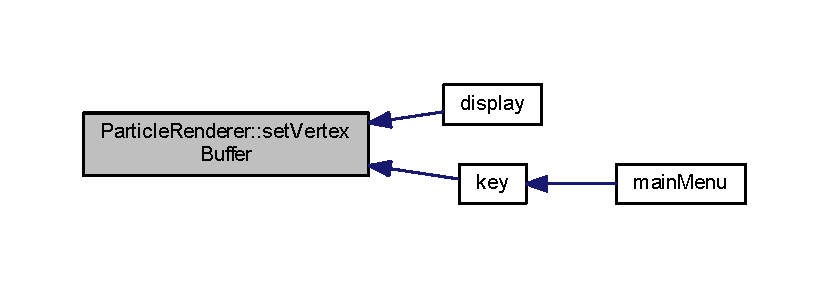
\includegraphics[width=350pt]{class_particle_renderer_a9c0d44ba7666ab432004a5df4cbb2b59_icgraph}
\end{center}
\end{figure}


\hypertarget{class_particle_renderer_ad84b464475e5ebd42cfed6e2e91e7247}{\index{Particle\-Renderer@{Particle\-Renderer}!set\-Window\-Size@{set\-Window\-Size}}
\index{set\-Window\-Size@{set\-Window\-Size}!ParticleRenderer@{Particle\-Renderer}}
\subsubsection[{set\-Window\-Size}]{\setlength{\rightskip}{0pt plus 5cm}void Particle\-Renderer\-::set\-Window\-Size (
\begin{DoxyParamCaption}
\item[{int}]{w, }
\item[{int}]{h}
\end{DoxyParamCaption}
)\hspace{0.3cm}{\ttfamily [inline]}}}\label{class_particle_renderer_ad84b464475e5ebd42cfed6e2e91e7247}


Definicja w linii \hyperlink{render__particles_8h_source_l00050}{50} pliku \hyperlink{render__particles_8h_source}{render\-\_\-particles.\-h}.



Odwołuje się do \hyperlink{render__particles_8h_source_l00068}{m\-\_\-window\-\_\-h} i \hyperlink{render__particles_8h_source_l00068}{m\-\_\-window\-\_\-w}.



Odwołania w \hyperlink{particles_8cpp_source_l00353}{reshape()}.


\begin{DoxyCode}
00051         \{
00052             \hyperlink{class_particle_renderer_aa71b7eba5d5665a086b7ba80adddf19b}{m\_window\_w} = w;
00053             \hyperlink{class_particle_renderer_af34b1e93f6a7f22774a6473c52027d77}{m\_window\_h} = h;
00054         \}
\end{DoxyCode}


Oto graf wywoływań tej funkcji\-:\nopagebreak
\begin{figure}[H]
\begin{center}
\leavevmode
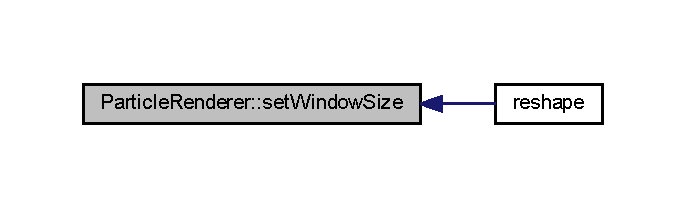
\includegraphics[width=329pt]{class_particle_renderer_ad84b464475e5ebd42cfed6e2e91e7247_icgraph}
\end{center}
\end{figure}




\subsection{Dokumentacja atrybutów składowych}
\hypertarget{class_particle_renderer_a7dcaa73a41c598207974432206b423b5}{\index{Particle\-Renderer@{Particle\-Renderer}!m\-\_\-color\-V\-B\-O@{m\-\_\-color\-V\-B\-O}}
\index{m\-\_\-color\-V\-B\-O@{m\-\_\-color\-V\-B\-O}!ParticleRenderer@{Particle\-Renderer}}
\subsubsection[{m\-\_\-color\-V\-B\-O}]{\setlength{\rightskip}{0pt plus 5cm}G\-Luint Particle\-Renderer\-::m\-\_\-color\-V\-B\-O\hspace{0.3cm}{\ttfamily [protected]}}}\label{class_particle_renderer_a7dcaa73a41c598207974432206b423b5}


Definicja w linii \hyperlink{render__particles_8h_source_l00073}{73} pliku \hyperlink{render__particles_8h_source}{render\-\_\-particles.\-h}.

\hypertarget{class_particle_renderer_a0aed003bd557a3c32ca7d2ca89fc59f7}{\index{Particle\-Renderer@{Particle\-Renderer}!m\-\_\-fov@{m\-\_\-fov}}
\index{m\-\_\-fov@{m\-\_\-fov}!ParticleRenderer@{Particle\-Renderer}}
\subsubsection[{m\-\_\-fov}]{\setlength{\rightskip}{0pt plus 5cm}float Particle\-Renderer\-::m\-\_\-fov\hspace{0.3cm}{\ttfamily [protected]}}}\label{class_particle_renderer_a0aed003bd557a3c32ca7d2ca89fc59f7}


Definicja w linii \hyperlink{render__particles_8h_source_l00067}{67} pliku \hyperlink{render__particles_8h_source}{render\-\_\-particles.\-h}.



Odwołania w \hyperlink{render__particles_8h_source_l00046}{set\-F\-O\-V()}.

\hypertarget{class_particle_renderer_af885fdb5e6da925209dfd960f66b5fd8}{\index{Particle\-Renderer@{Particle\-Renderer}!m\-\_\-num\-Particles@{m\-\_\-num\-Particles}}
\index{m\-\_\-num\-Particles@{m\-\_\-num\-Particles}!ParticleRenderer@{Particle\-Renderer}}
\subsubsection[{m\-\_\-num\-Particles}]{\setlength{\rightskip}{0pt plus 5cm}int Particle\-Renderer\-::m\-\_\-num\-Particles\hspace{0.3cm}{\ttfamily [protected]}}}\label{class_particle_renderer_af885fdb5e6da925209dfd960f66b5fd8}


Definicja w linii \hyperlink{render__particles_8h_source_l00063}{63} pliku \hyperlink{render__particles_8h_source}{render\-\_\-particles.\-h}.



Odwołania w \hyperlink{render__particles_8cpp_source_l00025}{Particle\-Renderer()}, \hyperlink{render__particles_8cpp_source_l00042}{set\-Positions()} i \hyperlink{render__particles_8cpp_source_l00048}{set\-Vertex\-Buffer()}.

\hypertarget{class_particle_renderer_aab5ee3cd769a64c45dc9714aabdb0ee2}{\index{Particle\-Renderer@{Particle\-Renderer}!m\-\_\-particle\-Radius@{m\-\_\-particle\-Radius}}
\index{m\-\_\-particle\-Radius@{m\-\_\-particle\-Radius}!ParticleRenderer@{Particle\-Renderer}}
\subsubsection[{m\-\_\-particle\-Radius}]{\setlength{\rightskip}{0pt plus 5cm}float Particle\-Renderer\-::m\-\_\-particle\-Radius\hspace{0.3cm}{\ttfamily [protected]}}}\label{class_particle_renderer_aab5ee3cd769a64c45dc9714aabdb0ee2}


Definicja w linii \hyperlink{render__particles_8h_source_l00066}{66} pliku \hyperlink{render__particles_8h_source}{render\-\_\-particles.\-h}.



Odwołania w \hyperlink{render__particles_8cpp_source_l00025}{Particle\-Renderer()} i \hyperlink{render__particles_8h_source_l00042}{set\-Particle\-Radius()}.

\hypertarget{class_particle_renderer_a1ca13e546c937cb546c0da19fa853b34}{\index{Particle\-Renderer@{Particle\-Renderer}!m\-\_\-point\-Size@{m\-\_\-point\-Size}}
\index{m\-\_\-point\-Size@{m\-\_\-point\-Size}!ParticleRenderer@{Particle\-Renderer}}
\subsubsection[{m\-\_\-point\-Size}]{\setlength{\rightskip}{0pt plus 5cm}float Particle\-Renderer\-::m\-\_\-point\-Size\hspace{0.3cm}{\ttfamily [protected]}}}\label{class_particle_renderer_a1ca13e546c937cb546c0da19fa853b34}


Definicja w linii \hyperlink{render__particles_8h_source_l00065}{65} pliku \hyperlink{render__particles_8h_source}{render\-\_\-particles.\-h}.



Odwołania w \hyperlink{render__particles_8cpp_source_l00025}{Particle\-Renderer()} i \hyperlink{render__particles_8h_source_l00038}{set\-Point\-Size()}.

\hypertarget{class_particle_renderer_a1d74720edb5c3a13edcdd176ac0d84c7}{\index{Particle\-Renderer@{Particle\-Renderer}!m\-\_\-pos@{m\-\_\-pos}}
\index{m\-\_\-pos@{m\-\_\-pos}!ParticleRenderer@{Particle\-Renderer}}
\subsubsection[{m\-\_\-pos}]{\setlength{\rightskip}{0pt plus 5cm}float$\ast$ Particle\-Renderer\-::m\-\_\-pos\hspace{0.3cm}{\ttfamily [protected]}}}\label{class_particle_renderer_a1d74720edb5c3a13edcdd176ac0d84c7}


Definicja w linii \hyperlink{render__particles_8h_source_l00062}{62} pliku \hyperlink{render__particles_8h_source}{render\-\_\-particles.\-h}.



Odwołania w \hyperlink{render__particles_8cpp_source_l00025}{Particle\-Renderer()}, \hyperlink{render__particles_8cpp_source_l00042}{set\-Positions()} i \hyperlink{render__particles_8cpp_source_l00037}{$\sim$\-Particle\-Renderer()}.

\hypertarget{class_particle_renderer_ab8f0dd1a6e0f4401012bd46ae8940648}{\index{Particle\-Renderer@{Particle\-Renderer}!m\-\_\-program@{m\-\_\-program}}
\index{m\-\_\-program@{m\-\_\-program}!ParticleRenderer@{Particle\-Renderer}}
\subsubsection[{m\-\_\-program}]{\setlength{\rightskip}{0pt plus 5cm}G\-Luint Particle\-Renderer\-::m\-\_\-program\hspace{0.3cm}{\ttfamily [protected]}}}\label{class_particle_renderer_ab8f0dd1a6e0f4401012bd46ae8940648}


Definicja w linii \hyperlink{render__particles_8h_source_l00070}{70} pliku \hyperlink{render__particles_8h_source}{render\-\_\-particles.\-h}.

\hypertarget{class_particle_renderer_a7549feaa0982abbc44c9fe73f2eb251f}{\index{Particle\-Renderer@{Particle\-Renderer}!m\-\_\-vbo@{m\-\_\-vbo}}
\index{m\-\_\-vbo@{m\-\_\-vbo}!ParticleRenderer@{Particle\-Renderer}}
\subsubsection[{m\-\_\-vbo}]{\setlength{\rightskip}{0pt plus 5cm}G\-Luint Particle\-Renderer\-::m\-\_\-vbo\hspace{0.3cm}{\ttfamily [protected]}}}\label{class_particle_renderer_a7549feaa0982abbc44c9fe73f2eb251f}


Definicja w linii \hyperlink{render__particles_8h_source_l00072}{72} pliku \hyperlink{render__particles_8h_source}{render\-\_\-particles.\-h}.

\hypertarget{class_particle_renderer_af34b1e93f6a7f22774a6473c52027d77}{\index{Particle\-Renderer@{Particle\-Renderer}!m\-\_\-window\-\_\-h@{m\-\_\-window\-\_\-h}}
\index{m\-\_\-window\-\_\-h@{m\-\_\-window\-\_\-h}!ParticleRenderer@{Particle\-Renderer}}
\subsubsection[{m\-\_\-window\-\_\-h}]{\setlength{\rightskip}{0pt plus 5cm}int Particle\-Renderer\-::m\-\_\-window\-\_\-h\hspace{0.3cm}{\ttfamily [protected]}}}\label{class_particle_renderer_af34b1e93f6a7f22774a6473c52027d77}


Definicja w linii \hyperlink{render__particles_8h_source_l00068}{68} pliku \hyperlink{render__particles_8h_source}{render\-\_\-particles.\-h}.



Odwołania w \hyperlink{render__particles_8h_source_l00050}{set\-Window\-Size()}.

\hypertarget{class_particle_renderer_aa71b7eba5d5665a086b7ba80adddf19b}{\index{Particle\-Renderer@{Particle\-Renderer}!m\-\_\-window\-\_\-w@{m\-\_\-window\-\_\-w}}
\index{m\-\_\-window\-\_\-w@{m\-\_\-window\-\_\-w}!ParticleRenderer@{Particle\-Renderer}}
\subsubsection[{m\-\_\-window\-\_\-w}]{\setlength{\rightskip}{0pt plus 5cm}int Particle\-Renderer\-::m\-\_\-window\-\_\-w\hspace{0.3cm}{\ttfamily [protected]}}}\label{class_particle_renderer_aa71b7eba5d5665a086b7ba80adddf19b}


Definicja w linii \hyperlink{render__particles_8h_source_l00068}{68} pliku \hyperlink{render__particles_8h_source}{render\-\_\-particles.\-h}.



Odwołania w \hyperlink{render__particles_8h_source_l00050}{set\-Window\-Size()}.



Dokumentacja dla tej klasy została wygenerowana z plików\-:\begin{DoxyCompactItemize}
\item 
\hyperlink{render__particles_8h}{render\-\_\-particles.\-h}\item 
\hyperlink{render__particles_8cpp}{render\-\_\-particles.\-cpp}\end{DoxyCompactItemize}

\hypertarget{class_particle_system}{\section{Dokumentacja klasy Particle\-System}
\label{class_particle_system}\index{Particle\-System@{Particle\-System}}
}


{\ttfamily \#include $<$particle\-System.\-h$>$}



Diagram współpracy dla Particle\-System\-:\nopagebreak
\begin{figure}[H]
\begin{center}
\leavevmode
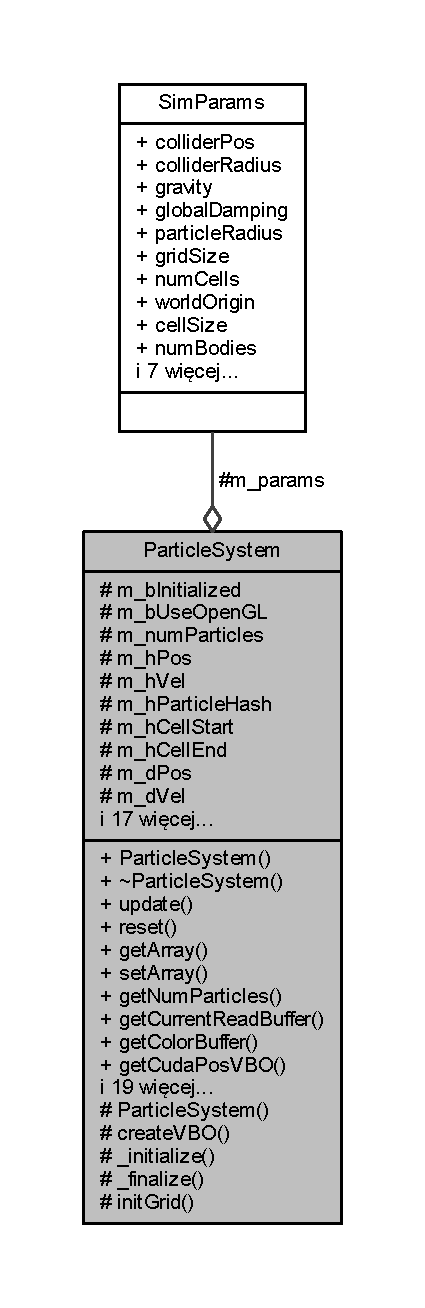
\includegraphics[height=550pt]{class_particle_system__coll__graph}
\end{center}
\end{figure}
\subsection*{Typy publiczne}
\begin{DoxyCompactItemize}
\item 
enum \hyperlink{class_particle_system_a1dca3996c8068602412ef9f7826605d1}{Particle\-Config} \{ \hyperlink{class_particle_system_a1dca3996c8068602412ef9f7826605d1a053c69e4e6b094605ea152a644e7c9ee}{C\-O\-N\-F\-I\-G\-\_\-\-R\-A\-N\-D\-O\-M}, 
\hyperlink{class_particle_system_a1dca3996c8068602412ef9f7826605d1aa6bd9e92edfc102877bf103547397b47}{C\-O\-N\-F\-I\-G\-\_\-\-G\-R\-I\-D}, 
\hyperlink{class_particle_system_a1dca3996c8068602412ef9f7826605d1a602c3604196d8513e85acf6fd039391e}{\-\_\-\-N\-U\-M\-\_\-\-C\-O\-N\-F\-I\-G\-S}
 \}
\item 
enum \hyperlink{class_particle_system_a332fbe57a36aaea5c18b4ea4fba6bbb3}{Particle\-Array} \{ \hyperlink{class_particle_system_a332fbe57a36aaea5c18b4ea4fba6bbb3a9e9a2992d230a2674debf26e0e8e0299}{P\-O\-S\-I\-T\-I\-O\-N}, 
\hyperlink{class_particle_system_a332fbe57a36aaea5c18b4ea4fba6bbb3a3702de73065f01b4f6ffa604b799e53d}{V\-E\-L\-O\-C\-I\-T\-Y}
 \}
\end{DoxyCompactItemize}
\subsection*{Metody publiczne}
\begin{DoxyCompactItemize}
\item 
\hyperlink{class_particle_system_a8a2be3e93616aa694801369c8b8d12cb}{Particle\-System} (\hyperlink{particles__kernel_8cuh_a91ad9478d81a7aaf2593e8d9c3d06a14}{uint} \hyperlink{particles_8cpp_a05b8a90212054a3eb1a036ae0c269596}{num\-Particles}, uint3 \hyperlink{particles_8cpp_aefe301f4cc6d6838e3627b5970e855a9}{grid\-Size}, bool b\-Use\-Open\-G\-L)
\item 
\hyperlink{class_particle_system_a6bc725349a763b9d6817950cde16a93f}{$\sim$\-Particle\-System} ()
\item 
void \hyperlink{class_particle_system_a166fd86f020b6024d7d42723762d7cb2}{update} (float delta\-Time)
\item 
void \hyperlink{class_particle_system_a519070812dd9eb349f270c793c5f64b6}{reset} (\hyperlink{class_particle_system_a1dca3996c8068602412ef9f7826605d1}{Particle\-Config} config)
\item 
float $\ast$ \hyperlink{class_particle_system_a8bdfaa6198651ef0ceb8be489ecd78e3}{get\-Array} (\hyperlink{class_particle_system_a332fbe57a36aaea5c18b4ea4fba6bbb3}{Particle\-Array} array)
\item 
void \hyperlink{class_particle_system_aa792a66680e800832059854aab0d594d}{set\-Array} (\hyperlink{class_particle_system_a332fbe57a36aaea5c18b4ea4fba6bbb3}{Particle\-Array} array, const float $\ast$data, int start, int count)
\item 
int \hyperlink{class_particle_system_a6f89e8d4c3e3e328088b7d652cee84b0}{get\-Num\-Particles} () const 
\item 
unsigned int \hyperlink{class_particle_system_ae9f149d6b7c3b148fc397473c7c3c2e2}{get\-Current\-Read\-Buffer} () const 
\item 
unsigned int \hyperlink{class_particle_system_a5d300a37ebf1a2fb8575f82ced6a208f}{get\-Color\-Buffer} () const 
\item 
void $\ast$ \hyperlink{class_particle_system_a2c8214a5bcd9d9c24d16e1f0063c06d6}{get\-Cuda\-Pos\-V\-B\-O} () const 
\item 
void $\ast$ \hyperlink{class_particle_system_af89375a9131276f941dccefa7840adda}{get\-Cuda\-Color\-V\-B\-O} () const 
\item 
void \hyperlink{class_particle_system_a722bdb7cc940f052400a69fe9569a49e}{dump\-Grid} ()
\item 
void \hyperlink{class_particle_system_a9025f319e07c58c6ece1cd2a620ce33a}{dump\-Particles} (\hyperlink{particles__kernel_8cuh_a91ad9478d81a7aaf2593e8d9c3d06a14}{uint} start, \hyperlink{particles__kernel_8cuh_a91ad9478d81a7aaf2593e8d9c3d06a14}{uint} count)
\item 
void \hyperlink{class_particle_system_a11f55976f6ef34dceea208fbe06694cd}{set\-Iterations} (int i)
\item 
void \hyperlink{class_particle_system_aa26996b9ca13499b13f944f3aaeae10c}{set\-Damping} (float x)
\item 
void \hyperlink{class_particle_system_a755f64f917389ef41df81b663d1f5bd2}{set\-Gravity} (float x)
\item 
void \hyperlink{class_particle_system_a7ed53fca9ef126898d29314478ec8fd4}{set\-Collide\-Spring} (float x)
\item 
void \hyperlink{class_particle_system_a8f8d21c7079c3a0e66558b9ec5bef597}{set\-Collide\-Damping} (float x)
\item 
void \hyperlink{class_particle_system_aea667093542a1bdad65bdcb427e5625f}{set\-Collide\-Shear} (float x)
\item 
void \hyperlink{class_particle_system_aef02d293e3dc61c50fa6d085aa0b03de}{set\-Collide\-Attraction} (float x)
\item 
void \hyperlink{class_particle_system_a97efe00aa29307ecae0165da33d4770a}{set\-Big\-Radius} (float x)
\item 
void \hyperlink{class_particle_system_a9c49794585cad649de400dc7375d7801}{set\-Collider\-Pos} (float3 x)
\item 
float \hyperlink{class_particle_system_abdb59a91d8483017ad71455bb2958993}{get\-Particle\-Radius} ()
\item 
float3 \hyperlink{class_particle_system_a3c8578d474f5a6f14d903a242aec96ec}{get\-Collider\-Pos} ()
\item 
float \hyperlink{class_particle_system_a56f07dfab9d5cbf510c6e0a28e816038}{get\-Collider\-Radius} ()
\item 
uint3 \hyperlink{class_particle_system_af94ba180bcb348afcfd81bb699d6aab0}{get\-Grid\-Size} ()
\item 
float3 \hyperlink{class_particle_system_a19d9bb799a5b5704d8fd6a286f6be20d}{get\-World\-Origin} ()
\item 
float3 \hyperlink{class_particle_system_a608bcb87f3d30fbfeae810da28ae1052}{get\-Cell\-Size} ()
\item 
void \hyperlink{class_particle_system_af2f16676fe8a0523cfb867a9a856970c}{add\-Sphere} (int index, float $\ast$pos, float $\ast$vel, int r, float spacing)
\end{DoxyCompactItemize}
\subsection*{Metody chronione}
\begin{DoxyCompactItemize}
\item 
\hyperlink{class_particle_system_a9028ec8023c61773dd4a668c3ad8cc26}{Particle\-System} ()
\item 
\hyperlink{particles__kernel_8cuh_a91ad9478d81a7aaf2593e8d9c3d06a14}{uint} \hyperlink{class_particle_system_a399eb5cb9c422fd3370899e4d8a5d62e}{create\-V\-B\-O} (\hyperlink{particles__kernel_8cuh_a91ad9478d81a7aaf2593e8d9c3d06a14}{uint} size)
\item 
void \hyperlink{class_particle_system_a484988642e046424d32a13709204e8de}{\-\_\-initialize} (int \hyperlink{particles_8cpp_a05b8a90212054a3eb1a036ae0c269596}{num\-Particles})
\item 
void \hyperlink{class_particle_system_a5d6a52db7d1277c8fe734ecceb69e5c6}{\-\_\-finalize} ()
\item 
void \hyperlink{class_particle_system_a2e08c4e354b0de5e2dc468a0fb457dfe}{init\-Grid} (\hyperlink{particles__kernel_8cuh_a91ad9478d81a7aaf2593e8d9c3d06a14}{uint} $\ast$size, float spacing, float jitter, \hyperlink{particles__kernel_8cuh_a91ad9478d81a7aaf2593e8d9c3d06a14}{uint} \hyperlink{particles_8cpp_a05b8a90212054a3eb1a036ae0c269596}{num\-Particles})
\end{DoxyCompactItemize}
\subsection*{Atrybuty chronione}
\begin{DoxyCompactItemize}
\item 
bool \hyperlink{class_particle_system_a21bbfba9d8701a70bc6fddbf4fc3f5bd}{m\-\_\-b\-Initialized}
\item 
bool \hyperlink{class_particle_system_a5d99413ffc0791e6aa9f02308caf7f1e}{m\-\_\-b\-Use\-Open\-G\-L}
\item 
\hyperlink{particles__kernel_8cuh_a91ad9478d81a7aaf2593e8d9c3d06a14}{uint} \hyperlink{class_particle_system_a23d238efa80a647d4b6cde034f486a91}{m\-\_\-num\-Particles}
\item 
float $\ast$ \hyperlink{class_particle_system_ab9d75471d2eaaeb8fa98d2f3f47d9c25}{m\-\_\-h\-Pos}
\item 
float $\ast$ \hyperlink{class_particle_system_a20560c896ee8a8bbc827a8e5902da7e2}{m\-\_\-h\-Vel}
\item 
\hyperlink{particles__kernel_8cuh_a91ad9478d81a7aaf2593e8d9c3d06a14}{uint} $\ast$ \hyperlink{class_particle_system_a4280ede7d75e44c8c0d4edfa5ee7dd02}{m\-\_\-h\-Particle\-Hash}
\item 
\hyperlink{particles__kernel_8cuh_a91ad9478d81a7aaf2593e8d9c3d06a14}{uint} $\ast$ \hyperlink{class_particle_system_a8412ecd991c14d906fcebba42bdeffd3}{m\-\_\-h\-Cell\-Start}
\item 
\hyperlink{particles__kernel_8cuh_a91ad9478d81a7aaf2593e8d9c3d06a14}{uint} $\ast$ \hyperlink{class_particle_system_a8d8ad2d142f3a5b83f2c10a46f5d7a8b}{m\-\_\-h\-Cell\-End}
\item 
float $\ast$ \hyperlink{class_particle_system_afff6217d2726217dff77c81ef3c23bfa}{m\-\_\-d\-Pos}
\item 
float $\ast$ \hyperlink{class_particle_system_a5efd31a2fdba8d98b105f4e546964cb5}{m\-\_\-d\-Vel}
\item 
float $\ast$ \hyperlink{class_particle_system_ab60e8b5a312b2f400b10dfba5153fc3c}{m\-\_\-d\-Sorted\-Pos}
\item 
float $\ast$ \hyperlink{class_particle_system_a69122523117954fb5defb8b38e0f46f3}{m\-\_\-d\-Sorted\-Vel}
\item 
\hyperlink{particles__kernel_8cuh_a91ad9478d81a7aaf2593e8d9c3d06a14}{uint} $\ast$ \hyperlink{class_particle_system_ab44080655971a5501eaee6ad7355a139}{m\-\_\-d\-Grid\-Particle\-Hash}
\item 
\hyperlink{particles__kernel_8cuh_a91ad9478d81a7aaf2593e8d9c3d06a14}{uint} $\ast$ \hyperlink{class_particle_system_a1a67fc1e3ffd4e64f55a2a315c49c74c}{m\-\_\-d\-Grid\-Particle\-Index}
\item 
\hyperlink{particles__kernel_8cuh_a91ad9478d81a7aaf2593e8d9c3d06a14}{uint} $\ast$ \hyperlink{class_particle_system_a137909a8b34f7a42e50cd0fcc86bb784}{m\-\_\-d\-Cell\-Start}
\item 
\hyperlink{particles__kernel_8cuh_a91ad9478d81a7aaf2593e8d9c3d06a14}{uint} $\ast$ \hyperlink{class_particle_system_a3a0b9c760c2bfcf811d54b8194ebea01}{m\-\_\-d\-Cell\-End}
\item 
\hyperlink{particles__kernel_8cuh_a91ad9478d81a7aaf2593e8d9c3d06a14}{uint} \hyperlink{class_particle_system_a2a0452a32993337176d88fa2fbe63020}{m\-\_\-grid\-Sort\-Bits}
\item 
\hyperlink{particles__kernel_8cuh_a91ad9478d81a7aaf2593e8d9c3d06a14}{uint} \hyperlink{class_particle_system_a31f9cccdf5dbae6f72867665bd8761e3}{m\-\_\-pos\-Vbo}
\item 
\hyperlink{particles__kernel_8cuh_a91ad9478d81a7aaf2593e8d9c3d06a14}{uint} \hyperlink{class_particle_system_a96b05c719006c9e3eaed759f54a49c7f}{m\-\_\-color\-V\-B\-O}
\item 
float $\ast$ \hyperlink{class_particle_system_aba18245745f621d90186862f1a559d9e}{m\-\_\-cuda\-Pos\-V\-B\-O}
\item 
float $\ast$ \hyperlink{class_particle_system_a39d210b57da5f7f4a2c23f4fc0b43ea1}{m\-\_\-cuda\-Color\-V\-B\-O}
\item 
struct cuda\-Graphics\-Resource $\ast$ \hyperlink{class_particle_system_a9c5de70c1705672e5722ad30dee1b14b}{m\-\_\-cuda\-\_\-posvbo\-\_\-resource}
\item 
struct cuda\-Graphics\-Resource $\ast$ \hyperlink{class_particle_system_a140043869727535abc08609b835b98fc}{m\-\_\-cuda\-\_\-colorvbo\-\_\-resource}
\item 
\hyperlink{struct_sim_params}{Sim\-Params} \hyperlink{class_particle_system_ab765472aed6a1b5f0d2f98a3a906c417}{m\-\_\-params}
\item 
uint3 \hyperlink{class_particle_system_ad555b31501a258d776e8c72c96178aa0}{m\-\_\-grid\-Size}
\item 
\hyperlink{particles__kernel_8cuh_a91ad9478d81a7aaf2593e8d9c3d06a14}{uint} \hyperlink{class_particle_system_aa1ef17d723af5d7a4685e8fd57e9ca89}{m\-\_\-num\-Grid\-Cells}
\item 
Stop\-Watch\-Interface $\ast$ \hyperlink{class_particle_system_af01e546384ef27bb1894a37f2a02e967}{m\-\_\-timer}
\item 
\hyperlink{particles__kernel_8cuh_a91ad9478d81a7aaf2593e8d9c3d06a14}{uint} \hyperlink{class_particle_system_a7b4b053433c052518b8ecce1b02000f5}{m\-\_\-solver\-Iterations}
\end{DoxyCompactItemize}


\subsection{Opis szczegółowy}


Definicja w linii \hyperlink{particle_system_8h_source_l00023}{23} pliku \hyperlink{particle_system_8h_source}{particle\-System.\-h}.



\subsection{Dokumentacja składowych wyliczanych}
\hypertarget{class_particle_system_a332fbe57a36aaea5c18b4ea4fba6bbb3}{\index{Particle\-System@{Particle\-System}!Particle\-Array@{Particle\-Array}}
\index{Particle\-Array@{Particle\-Array}!ParticleSystem@{Particle\-System}}
\subsubsection[{Particle\-Array}]{\setlength{\rightskip}{0pt plus 5cm}enum {\bf Particle\-System\-::\-Particle\-Array}}}\label{class_particle_system_a332fbe57a36aaea5c18b4ea4fba6bbb3}
\begin{Desc}
\item[Wartości wyliczeń]\par
\begin{description}
\index{P\-O\-S\-I\-T\-I\-O\-N@{P\-O\-S\-I\-T\-I\-O\-N}!Particle\-System@{Particle\-System}}\index{Particle\-System@{Particle\-System}!P\-O\-S\-I\-T\-I\-O\-N@{P\-O\-S\-I\-T\-I\-O\-N}}\item[{\em 
\hypertarget{class_particle_system_a332fbe57a36aaea5c18b4ea4fba6bbb3a9e9a2992d230a2674debf26e0e8e0299}{P\-O\-S\-I\-T\-I\-O\-N}\label{class_particle_system_a332fbe57a36aaea5c18b4ea4fba6bbb3a9e9a2992d230a2674debf26e0e8e0299}
}]\index{V\-E\-L\-O\-C\-I\-T\-Y@{V\-E\-L\-O\-C\-I\-T\-Y}!Particle\-System@{Particle\-System}}\index{Particle\-System@{Particle\-System}!V\-E\-L\-O\-C\-I\-T\-Y@{V\-E\-L\-O\-C\-I\-T\-Y}}\item[{\em 
\hypertarget{class_particle_system_a332fbe57a36aaea5c18b4ea4fba6bbb3a3702de73065f01b4f6ffa604b799e53d}{V\-E\-L\-O\-C\-I\-T\-Y}\label{class_particle_system_a332fbe57a36aaea5c18b4ea4fba6bbb3a3702de73065f01b4f6ffa604b799e53d}
}]\end{description}
\end{Desc}


Definicja w linii \hyperlink{particle_system_8h_source_l00036}{36} pliku \hyperlink{particle_system_8h_source}{particle\-System.\-h}.


\begin{DoxyCode}
00037         \{
00038             \hyperlink{class_particle_system_a332fbe57a36aaea5c18b4ea4fba6bbb3a9e9a2992d230a2674debf26e0e8e0299}{POSITION},
00039             \hyperlink{class_particle_system_a332fbe57a36aaea5c18b4ea4fba6bbb3a3702de73065f01b4f6ffa604b799e53d}{VELOCITY},
00040         \};
\end{DoxyCode}
\hypertarget{class_particle_system_a1dca3996c8068602412ef9f7826605d1}{\index{Particle\-System@{Particle\-System}!Particle\-Config@{Particle\-Config}}
\index{Particle\-Config@{Particle\-Config}!ParticleSystem@{Particle\-System}}
\subsubsection[{Particle\-Config}]{\setlength{\rightskip}{0pt plus 5cm}enum {\bf Particle\-System\-::\-Particle\-Config}}}\label{class_particle_system_a1dca3996c8068602412ef9f7826605d1}
\begin{Desc}
\item[Wartości wyliczeń]\par
\begin{description}
\index{C\-O\-N\-F\-I\-G\-\_\-\-R\-A\-N\-D\-O\-M@{C\-O\-N\-F\-I\-G\-\_\-\-R\-A\-N\-D\-O\-M}!Particle\-System@{Particle\-System}}\index{Particle\-System@{Particle\-System}!C\-O\-N\-F\-I\-G\-\_\-\-R\-A\-N\-D\-O\-M@{C\-O\-N\-F\-I\-G\-\_\-\-R\-A\-N\-D\-O\-M}}\item[{\em 
\hypertarget{class_particle_system_a1dca3996c8068602412ef9f7826605d1a053c69e4e6b094605ea152a644e7c9ee}{C\-O\-N\-F\-I\-G\-\_\-\-R\-A\-N\-D\-O\-M}\label{class_particle_system_a1dca3996c8068602412ef9f7826605d1a053c69e4e6b094605ea152a644e7c9ee}
}]\index{C\-O\-N\-F\-I\-G\-\_\-\-G\-R\-I\-D@{C\-O\-N\-F\-I\-G\-\_\-\-G\-R\-I\-D}!Particle\-System@{Particle\-System}}\index{Particle\-System@{Particle\-System}!C\-O\-N\-F\-I\-G\-\_\-\-G\-R\-I\-D@{C\-O\-N\-F\-I\-G\-\_\-\-G\-R\-I\-D}}\item[{\em 
\hypertarget{class_particle_system_a1dca3996c8068602412ef9f7826605d1aa6bd9e92edfc102877bf103547397b47}{C\-O\-N\-F\-I\-G\-\_\-\-G\-R\-I\-D}\label{class_particle_system_a1dca3996c8068602412ef9f7826605d1aa6bd9e92edfc102877bf103547397b47}
}]\index{\-\_\-\-N\-U\-M\-\_\-\-C\-O\-N\-F\-I\-G\-S@{\-\_\-\-N\-U\-M\-\_\-\-C\-O\-N\-F\-I\-G\-S}!Particle\-System@{Particle\-System}}\index{Particle\-System@{Particle\-System}!\-\_\-\-N\-U\-M\-\_\-\-C\-O\-N\-F\-I\-G\-S@{\-\_\-\-N\-U\-M\-\_\-\-C\-O\-N\-F\-I\-G\-S}}\item[{\em 
\hypertarget{class_particle_system_a1dca3996c8068602412ef9f7826605d1a602c3604196d8513e85acf6fd039391e}{\-\_\-\-N\-U\-M\-\_\-\-C\-O\-N\-F\-I\-G\-S}\label{class_particle_system_a1dca3996c8068602412ef9f7826605d1a602c3604196d8513e85acf6fd039391e}
}]\end{description}
\end{Desc}


Definicja w linii \hyperlink{particle_system_8h_source_l00029}{29} pliku \hyperlink{particle_system_8h_source}{particle\-System.\-h}.


\begin{DoxyCode}
00030         \{
00031             \hyperlink{class_particle_system_a1dca3996c8068602412ef9f7826605d1a053c69e4e6b094605ea152a644e7c9ee}{CONFIG\_RANDOM},
00032             \hyperlink{class_particle_system_a1dca3996c8068602412ef9f7826605d1aa6bd9e92edfc102877bf103547397b47}{CONFIG\_GRID},
00033             \hyperlink{class_particle_system_a1dca3996c8068602412ef9f7826605d1a602c3604196d8513e85acf6fd039391e}{\_NUM\_CONFIGS}
00034         \};
\end{DoxyCode}


\subsection{Dokumentacja konstruktora i destruktora}
\hypertarget{class_particle_system_a8a2be3e93616aa694801369c8b8d12cb}{\index{Particle\-System@{Particle\-System}!Particle\-System@{Particle\-System}}
\index{Particle\-System@{Particle\-System}!ParticleSystem@{Particle\-System}}
\subsubsection[{Particle\-System}]{\setlength{\rightskip}{0pt plus 5cm}Particle\-System\-::\-Particle\-System (
\begin{DoxyParamCaption}
\item[{{\bf uint}}]{num\-Particles, }
\item[{uint3}]{grid\-Size, }
\item[{bool}]{b\-Use\-Open\-G\-L}
\end{DoxyParamCaption}
)}}\label{class_particle_system_a8a2be3e93616aa694801369c8b8d12cb}


Definicja w linii \hyperlink{particle_system_8cpp_source_l00033}{33} pliku \hyperlink{particle_system_8cpp_source}{particle\-System.\-cpp}.



Odwołuje się do \hyperlink{particle_system_8cpp_source_l00123}{\-\_\-initialize()}, \hyperlink{particle_system_8h_source_l00152}{m\-\_\-b\-Initialized}, \hyperlink{particle_system_8h_source_l00152}{m\-\_\-b\-Use\-Open\-G\-L}, \hyperlink{particle_system_8h_source_l00164}{m\-\_\-d\-Pos}, \hyperlink{particle_system_8h_source_l00165}{m\-\_\-d\-Vel}, \hyperlink{particle_system_8h_source_l00176}{m\-\_\-grid\-Sort\-Bits}, \hyperlink{particle_system_8h_source_l00156}{m\-\_\-h\-Pos}, \hyperlink{particle_system_8h_source_l00157}{m\-\_\-h\-Vel}, \hyperlink{particle_system_8h_source_l00153}{m\-\_\-num\-Particles}, \hyperlink{particle_system_8h_source_l00194}{m\-\_\-solver\-Iterations} i \hyperlink{particle_system_8cpp_source_l00033}{Particle\-System()}.



Odwołania w \hyperlink{particle_system_8cpp_source_l00033}{Particle\-System()}.


\begin{DoxyCode}
00033                                                                                  :
00034     \hyperlink{class_particle_system_a21bbfba9d8701a70bc6fddbf4fc3f5bd}{m\_bInitialized}(\textcolor{keyword}{false}),
00035     \hyperlink{class_particle_system_a5d99413ffc0791e6aa9f02308caf7f1e}{m\_bUseOpenGL}(bUseOpenGL),
00036     \hyperlink{class_particle_system_a23d238efa80a647d4b6cde034f486a91}{m\_numParticles}(\hyperlink{particles_8cpp_a05b8a90212054a3eb1a036ae0c269596}{numParticles}),
00037     \hyperlink{class_particle_system_ab9d75471d2eaaeb8fa98d2f3f47d9c25}{m\_hPos}(0),
00038     \hyperlink{class_particle_system_a20560c896ee8a8bbc827a8e5902da7e2}{m\_hVel}(0),
00039     \hyperlink{class_particle_system_afff6217d2726217dff77c81ef3c23bfa}{m\_dPos}(0),
00040     \hyperlink{class_particle_system_a5efd31a2fdba8d98b105f4e546964cb5}{m\_dVel}(0),
00041     \hyperlink{class_particle_system_ad555b31501a258d776e8c72c96178aa0}{m\_gridSize}(\hyperlink{particles_8cpp_aefe301f4cc6d6838e3627b5970e855a9}{gridSize}),
00042     \hyperlink{class_particle_system_af01e546384ef27bb1894a37f2a02e967}{m\_timer}(NULL),
00043     \hyperlink{class_particle_system_a7b4b053433c052518b8ecce1b02000f5}{m\_solverIterations}(1)
00044 \{
00045     \hyperlink{class_particle_system_aa1ef17d723af5d7a4685e8fd57e9ca89}{m\_numGridCells} = \hyperlink{class_particle_system_ad555b31501a258d776e8c72c96178aa0}{m\_gridSize}.x*\hyperlink{class_particle_system_ad555b31501a258d776e8c72c96178aa0}{m\_gridSize}.y*
      \hyperlink{class_particle_system_ad555b31501a258d776e8c72c96178aa0}{m\_gridSize}.z;
00046     float3 worldSize = make\_float3(2.0f, 2.0f, 2.0f);
00047 
00048     \hyperlink{class_particle_system_a2a0452a32993337176d88fa2fbe63020}{m\_gridSortBits} = 18;    \textcolor{comment}{// increase this for larger grids}
00049 
00050     \textcolor{comment}{// set simulation parameters}
00051     \hyperlink{class_particle_system_ab765472aed6a1b5f0d2f98a3a906c417}{m\_params}.\hyperlink{struct_sim_params_a4cfb18ff777876da3ad69aae6e023949}{gridSize} = \hyperlink{class_particle_system_ad555b31501a258d776e8c72c96178aa0}{m\_gridSize};
00052     \hyperlink{class_particle_system_ab765472aed6a1b5f0d2f98a3a906c417}{m\_params}.\hyperlink{struct_sim_params_a9d51112b7e86d46b6f33126a67cc84b4}{numCells} = \hyperlink{class_particle_system_aa1ef17d723af5d7a4685e8fd57e9ca89}{m\_numGridCells};
00053     \hyperlink{class_particle_system_ab765472aed6a1b5f0d2f98a3a906c417}{m\_params}.\hyperlink{struct_sim_params_adb68e9ee2422208807756b367efdf842}{numBodies} = \hyperlink{class_particle_system_a23d238efa80a647d4b6cde034f486a91}{m\_numParticles};
00054 
00055     \hyperlink{class_particle_system_ab765472aed6a1b5f0d2f98a3a906c417}{m\_params}.\hyperlink{struct_sim_params_a7e131c24e1020c44173deb0f57a8c4af}{particleRadius} = 1.0f / 64.0f;\textcolor{comment}{//32.0f / 64.0f;}
00056     \hyperlink{class_particle_system_ab765472aed6a1b5f0d2f98a3a906c417}{m\_params}.\hyperlink{struct_sim_params_aa27be265020f137f0a9cfbc3f1d2d9f8}{colliderPos} = make\_float3(-1.2f, -0.8f, 0.8f);
00057     \hyperlink{class_particle_system_ab765472aed6a1b5f0d2f98a3a906c417}{m\_params}.\hyperlink{struct_sim_params_a06ca2162f6f0aec08343db6ed8cd4478}{colliderRadius} = 0.2f;
00058 
00059     \hyperlink{class_particle_system_ab765472aed6a1b5f0d2f98a3a906c417}{m\_params}.\hyperlink{struct_sim_params_a1ed7465773f15f2874650f19cec3d0a9}{worldOrigin} = make\_float3(-1.0f, -1.0f, -1.0f);
00060     \textcolor{comment}{//    m\_params.cellSize = make\_float3(worldSize.x / m\_gridSize.x, worldSize.y / m\_gridSize.y,
       worldSize.z / m\_gridSize.z);}
00061     \textcolor{keywordtype}{float} cellSize = \hyperlink{class_particle_system_ab765472aed6a1b5f0d2f98a3a906c417}{m\_params}.\hyperlink{struct_sim_params_a7e131c24e1020c44173deb0f57a8c4af}{particleRadius} * 2.0f;  \textcolor{comment}{// cell size equal to particle
       diameter}
00062     \hyperlink{class_particle_system_ab765472aed6a1b5f0d2f98a3a906c417}{m\_params}.\hyperlink{struct_sim_params_ad5d71ad4ba6acc829a35f47b3da3e169}{cellSize} = make\_float3(cellSize, cellSize, cellSize);
00063 
00064     \hyperlink{class_particle_system_ab765472aed6a1b5f0d2f98a3a906c417}{m\_params}.\hyperlink{struct_sim_params_a301314921adc7bce20d8955cf03cdf3f}{spring} = 0.5f;
00065     \hyperlink{class_particle_system_ab765472aed6a1b5f0d2f98a3a906c417}{m\_params}.\hyperlink{struct_sim_params_abf1644c671e60ebaf873d9167e755328}{damping} = 0.02f;
00066     \hyperlink{class_particle_system_ab765472aed6a1b5f0d2f98a3a906c417}{m\_params}.\hyperlink{struct_sim_params_ad48210724ada15a14a649b25ad61575b}{shear} = 0.1f;
00067     \hyperlink{class_particle_system_ab765472aed6a1b5f0d2f98a3a906c417}{m\_params}.\hyperlink{struct_sim_params_acf7442ae8a49237861944271cb630d01}{attraction} = 0.1f;
00068     \hyperlink{class_particle_system_ab765472aed6a1b5f0d2f98a3a906c417}{m\_params}.\hyperlink{struct_sim_params_a4da0c7593d6569e48ee50e7d0c7576f9}{boundaryDamping} = -0.1f;
00069 
00070     \hyperlink{class_particle_system_ab765472aed6a1b5f0d2f98a3a906c417}{m\_params}.\hyperlink{struct_sim_params_ae7508eba5dd90859215b59d19e001bb9}{gravity} = make\_float3(0.0f, -0.0003f, 0.0f);
00071     \hyperlink{class_particle_system_ab765472aed6a1b5f0d2f98a3a906c417}{m\_params}.\hyperlink{struct_sim_params_a7058bad8c867d9d42d8c9d842638ebea}{globalDamping} = 1.0f;
00072 
00073         \hyperlink{class_particle_system_ab765472aed6a1b5f0d2f98a3a906c417}{m\_params}.\hyperlink{struct_sim_params_af41979948fdd8f76fe28ce2b43eb24cd}{bigradius}=2.0f;\textcolor{comment}{//docelowo zmieny rozmiar zewnetrznej kuli}
00074 
00075     \hyperlink{class_particle_system_a484988642e046424d32a13709204e8de}{\_initialize}(\hyperlink{particles_8cpp_a05b8a90212054a3eb1a036ae0c269596}{numParticles});
00076 \}
\end{DoxyCode}


Oto graf wywołań dla tej funkcji\-:\nopagebreak
\begin{figure}[H]
\begin{center}
\leavevmode
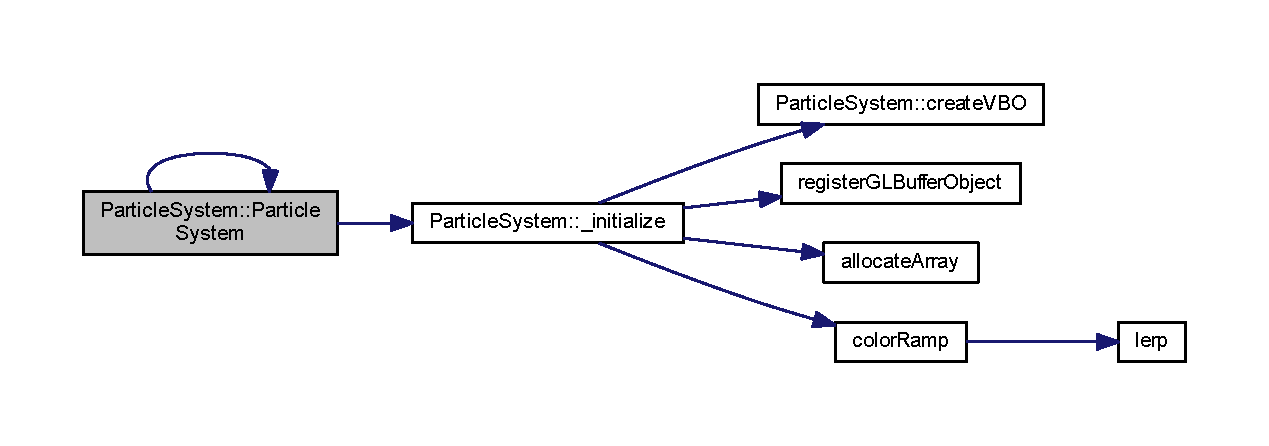
\includegraphics[width=350pt]{class_particle_system_a8a2be3e93616aa694801369c8b8d12cb_cgraph}
\end{center}
\end{figure}




Oto graf wywoływań tej funkcji\-:\nopagebreak
\begin{figure}[H]
\begin{center}
\leavevmode
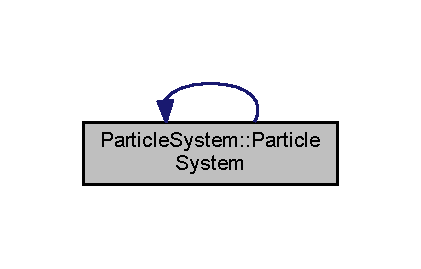
\includegraphics[width=202pt]{class_particle_system_a8a2be3e93616aa694801369c8b8d12cb_icgraph}
\end{center}
\end{figure}


\hypertarget{class_particle_system_a6bc725349a763b9d6817950cde16a93f}{\index{Particle\-System@{Particle\-System}!$\sim$\-Particle\-System@{$\sim$\-Particle\-System}}
\index{$\sim$\-Particle\-System@{$\sim$\-Particle\-System}!ParticleSystem@{Particle\-System}}
\subsubsection[{$\sim$\-Particle\-System}]{\setlength{\rightskip}{0pt plus 5cm}Particle\-System\-::$\sim$\-Particle\-System (
\begin{DoxyParamCaption}
{}
\end{DoxyParamCaption}
)}}\label{class_particle_system_a6bc725349a763b9d6817950cde16a93f}


Definicja w linii \hyperlink{particle_system_8cpp_source_l00078}{78} pliku \hyperlink{particle_system_8cpp_source}{particle\-System.\-cpp}.



Odwołuje się do \hyperlink{particle_system_8cpp_source_l00205}{\-\_\-finalize()} i \hyperlink{particle_system_8h_source_l00153}{m\-\_\-num\-Particles}.


\begin{DoxyCode}
00079 \{
00080     \hyperlink{class_particle_system_a5d6a52db7d1277c8fe734ecceb69e5c6}{\_finalize}();
00081     \hyperlink{class_particle_system_a23d238efa80a647d4b6cde034f486a91}{m\_numParticles} = 0;
00082 \}
\end{DoxyCode}


Oto graf wywołań dla tej funkcji\-:\nopagebreak
\begin{figure}[H]
\begin{center}
\leavevmode
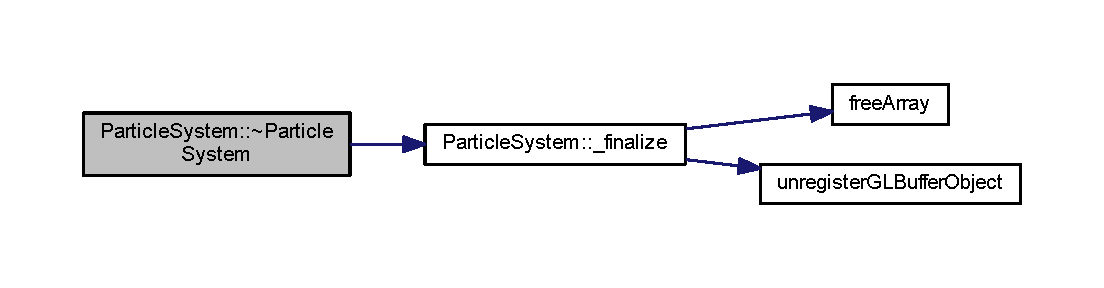
\includegraphics[width=350pt]{class_particle_system_a6bc725349a763b9d6817950cde16a93f_cgraph}
\end{center}
\end{figure}


\hypertarget{class_particle_system_a9028ec8023c61773dd4a668c3ad8cc26}{\index{Particle\-System@{Particle\-System}!Particle\-System@{Particle\-System}}
\index{Particle\-System@{Particle\-System}!ParticleSystem@{Particle\-System}}
\subsubsection[{Particle\-System}]{\setlength{\rightskip}{0pt plus 5cm}Particle\-System\-::\-Particle\-System (
\begin{DoxyParamCaption}
{}
\end{DoxyParamCaption}
)\hspace{0.3cm}{\ttfamily [inline]}, {\ttfamily [protected]}}}\label{class_particle_system_a9028ec8023c61773dd4a668c3ad8cc26}


Definicja w linii \hyperlink{particle_system_8h_source_l00143}{143} pliku \hyperlink{particle_system_8h_source}{particle\-System.\-h}.


\begin{DoxyCode}
00143 \{\}
\end{DoxyCode}


\subsection{Dokumentacja funkcji składowych}
\hypertarget{class_particle_system_a5d6a52db7d1277c8fe734ecceb69e5c6}{\index{Particle\-System@{Particle\-System}!\-\_\-finalize@{\-\_\-finalize}}
\index{\-\_\-finalize@{\-\_\-finalize}!ParticleSystem@{Particle\-System}}
\subsubsection[{\-\_\-finalize}]{\setlength{\rightskip}{0pt plus 5cm}void Particle\-System\-::\-\_\-finalize (
\begin{DoxyParamCaption}
{}
\end{DoxyParamCaption}
)\hspace{0.3cm}{\ttfamily [protected]}}}\label{class_particle_system_a5d6a52db7d1277c8fe734ecceb69e5c6}


Definicja w linii \hyperlink{particle_system_8cpp_source_l00205}{205} pliku \hyperlink{particle_system_8cpp_source}{particle\-System.\-cpp}.



Odwołuje się do \hyperlink{particle_system__cuda_8cu_source_l00067}{free\-Array()}, \hyperlink{particle_system_8h_source_l00152}{m\-\_\-b\-Initialized}, \hyperlink{particle_system_8h_source_l00152}{m\-\_\-b\-Use\-Open\-G\-L}, \hyperlink{particle_system_8h_source_l00184}{m\-\_\-cuda\-\_\-posvbo\-\_\-resource}, \hyperlink{particle_system_8h_source_l00174}{m\-\_\-d\-Cell\-End}, \hyperlink{particle_system_8h_source_l00173}{m\-\_\-d\-Cell\-Start}, \hyperlink{particle_system_8h_source_l00171}{m\-\_\-d\-Grid\-Particle\-Hash}, \hyperlink{particle_system_8h_source_l00172}{m\-\_\-d\-Grid\-Particle\-Index}, \hyperlink{particle_system_8h_source_l00167}{m\-\_\-d\-Sorted\-Pos}, \hyperlink{particle_system_8h_source_l00168}{m\-\_\-d\-Sorted\-Vel}, \hyperlink{particle_system_8h_source_l00165}{m\-\_\-d\-Vel}, \hyperlink{particle_system_8h_source_l00161}{m\-\_\-h\-Cell\-End}, \hyperlink{particle_system_8h_source_l00160}{m\-\_\-h\-Cell\-Start}, \hyperlink{particle_system_8h_source_l00156}{m\-\_\-h\-Pos}, \hyperlink{particle_system_8h_source_l00157}{m\-\_\-h\-Vel} i \hyperlink{particle_system__cuda_8cu_source_l00088}{unregister\-G\-L\-Buffer\-Object()}.



Odwołania w \hyperlink{particle_system_8cpp_source_l00078}{$\sim$\-Particle\-System()}.


\begin{DoxyCode}
00206 \{
00207     assert(\hyperlink{class_particle_system_a21bbfba9d8701a70bc6fddbf4fc3f5bd}{m\_bInitialized});
00208 
00209     \textcolor{keyword}{delete} [] \hyperlink{class_particle_system_ab9d75471d2eaaeb8fa98d2f3f47d9c25}{m\_hPos};
00210     \textcolor{keyword}{delete} [] \hyperlink{class_particle_system_a20560c896ee8a8bbc827a8e5902da7e2}{m\_hVel};
00211     \textcolor{keyword}{delete} [] \hyperlink{class_particle_system_a8412ecd991c14d906fcebba42bdeffd3}{m\_hCellStart};
00212     \textcolor{keyword}{delete} [] \hyperlink{class_particle_system_a8d8ad2d142f3a5b83f2c10a46f5d7a8b}{m\_hCellEnd};
00213 
00214     \hyperlink{particle_system_8cuh_a2946519c8d9c4f8ebf552bf044821ea9}{freeArray}(\hyperlink{class_particle_system_a5efd31a2fdba8d98b105f4e546964cb5}{m\_dVel});
00215     \hyperlink{particle_system_8cuh_a2946519c8d9c4f8ebf552bf044821ea9}{freeArray}(\hyperlink{class_particle_system_ab60e8b5a312b2f400b10dfba5153fc3c}{m\_dSortedPos});
00216     \hyperlink{particle_system_8cuh_a2946519c8d9c4f8ebf552bf044821ea9}{freeArray}(\hyperlink{class_particle_system_a69122523117954fb5defb8b38e0f46f3}{m\_dSortedVel});
00217 
00218     \hyperlink{particle_system_8cuh_a2946519c8d9c4f8ebf552bf044821ea9}{freeArray}(\hyperlink{class_particle_system_ab44080655971a5501eaee6ad7355a139}{m\_dGridParticleHash});
00219     \hyperlink{particle_system_8cuh_a2946519c8d9c4f8ebf552bf044821ea9}{freeArray}(\hyperlink{class_particle_system_a1a67fc1e3ffd4e64f55a2a315c49c74c}{m\_dGridParticleIndex});
00220     \hyperlink{particle_system_8cuh_a2946519c8d9c4f8ebf552bf044821ea9}{freeArray}(\hyperlink{class_particle_system_a137909a8b34f7a42e50cd0fcc86bb784}{m\_dCellStart});
00221     \hyperlink{particle_system_8cuh_a2946519c8d9c4f8ebf552bf044821ea9}{freeArray}(\hyperlink{class_particle_system_a3a0b9c760c2bfcf811d54b8194ebea01}{m\_dCellEnd});
00222 
00223     \textcolor{keywordflow}{if} (\hyperlink{class_particle_system_a5d99413ffc0791e6aa9f02308caf7f1e}{m\_bUseOpenGL})
00224     \{
00225         \hyperlink{particle_system_8cuh_a9afef8c00ca779aae2d7484b45bce34c}{unregisterGLBufferObject}(\hyperlink{class_particle_system_a9c5de70c1705672e5722ad30dee1b14b}{m\_cuda\_posvbo\_resource});
00226         glDeleteBuffers(1, (\textcolor{keyword}{const} GLuint *)&\hyperlink{class_particle_system_a31f9cccdf5dbae6f72867665bd8761e3}{m\_posVbo});
00227         glDeleteBuffers(1, (\textcolor{keyword}{const} GLuint *)&\hyperlink{class_particle_system_a96b05c719006c9e3eaed759f54a49c7f}{m\_colorVBO});
00228     \}
00229     \textcolor{keywordflow}{else}
00230     \{
00231         checkCudaErrors(cudaFree(\hyperlink{class_particle_system_aba18245745f621d90186862f1a559d9e}{m\_cudaPosVBO}));
00232         checkCudaErrors(cudaFree(\hyperlink{class_particle_system_a39d210b57da5f7f4a2c23f4fc0b43ea1}{m\_cudaColorVBO}));
00233     \}
00234 \}
\end{DoxyCode}


Oto graf wywołań dla tej funkcji\-:\nopagebreak
\begin{figure}[H]
\begin{center}
\leavevmode
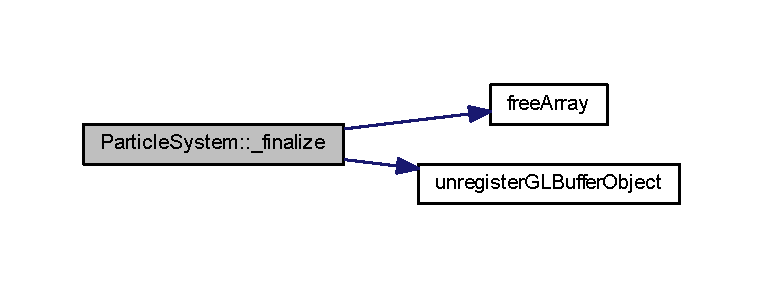
\includegraphics[width=350pt]{class_particle_system_a5d6a52db7d1277c8fe734ecceb69e5c6_cgraph}
\end{center}
\end{figure}




Oto graf wywoływań tej funkcji\-:\nopagebreak
\begin{figure}[H]
\begin{center}
\leavevmode
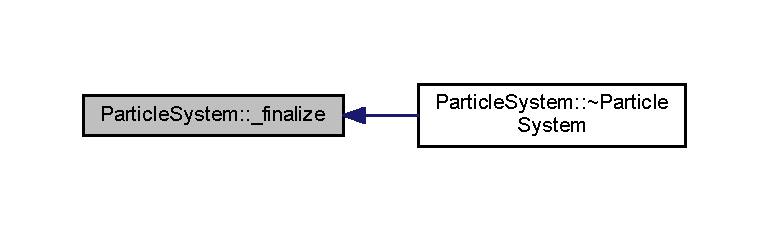
\includegraphics[width=350pt]{class_particle_system_a5d6a52db7d1277c8fe734ecceb69e5c6_icgraph}
\end{center}
\end{figure}


\hypertarget{class_particle_system_a484988642e046424d32a13709204e8de}{\index{Particle\-System@{Particle\-System}!\-\_\-initialize@{\-\_\-initialize}}
\index{\-\_\-initialize@{\-\_\-initialize}!ParticleSystem@{Particle\-System}}
\subsubsection[{\-\_\-initialize}]{\setlength{\rightskip}{0pt plus 5cm}void Particle\-System\-::\-\_\-initialize (
\begin{DoxyParamCaption}
\item[{int}]{num\-Particles}
\end{DoxyParamCaption}
)\hspace{0.3cm}{\ttfamily [protected]}}}\label{class_particle_system_a484988642e046424d32a13709204e8de}


Definicja w linii \hyperlink{particle_system_8cpp_source_l00123}{123} pliku \hyperlink{particle_system_8cpp_source}{particle\-System.\-cpp}.



Odwołuje się do \hyperlink{particle_system_8cuh_aee51e01a5233e0fda578bd5b3bc38e8f}{allocate\-Array()}, \hyperlink{particle_system_8cpp_source_l00101}{color\-Ramp()}, \hyperlink{particle_system_8cpp_source_l00085}{create\-V\-B\-O()}, \hyperlink{particle_system_8h_source_l00152}{m\-\_\-b\-Initialized}, \hyperlink{particle_system_8h_source_l00152}{m\-\_\-b\-Use\-Open\-G\-L}, \hyperlink{particle_system_8h_source_l00179}{m\-\_\-color\-V\-B\-O}, \hyperlink{particle_system_8h_source_l00185}{m\-\_\-cuda\-\_\-colorvbo\-\_\-resource}, \hyperlink{particle_system_8h_source_l00184}{m\-\_\-cuda\-\_\-posvbo\-\_\-resource}, \hyperlink{particle_system_8h_source_l00174}{m\-\_\-d\-Cell\-End}, \hyperlink{particle_system_8h_source_l00173}{m\-\_\-d\-Cell\-Start}, \hyperlink{particle_system_8h_source_l00171}{m\-\_\-d\-Grid\-Particle\-Hash}, \hyperlink{particle_system_8h_source_l00172}{m\-\_\-d\-Grid\-Particle\-Index}, \hyperlink{particle_system_8h_source_l00167}{m\-\_\-d\-Sorted\-Pos}, \hyperlink{particle_system_8h_source_l00168}{m\-\_\-d\-Sorted\-Vel}, \hyperlink{particle_system_8h_source_l00165}{m\-\_\-d\-Vel}, \hyperlink{particle_system_8h_source_l00161}{m\-\_\-h\-Cell\-End}, \hyperlink{particle_system_8h_source_l00160}{m\-\_\-h\-Cell\-Start}, \hyperlink{particle_system_8h_source_l00156}{m\-\_\-h\-Pos}, \hyperlink{particle_system_8h_source_l00157}{m\-\_\-h\-Vel}, \hyperlink{particle_system_8h_source_l00190}{m\-\_\-num\-Grid\-Cells}, \hyperlink{particle_system_8h_source_l00153}{m\-\_\-num\-Particles}, \hyperlink{particle_system_8h_source_l00178}{m\-\_\-pos\-Vbo} i \hyperlink{particle_system__cuda_8cu_source_l00082}{register\-G\-L\-Buffer\-Object()}.



Odwołania w \hyperlink{particle_system_8cpp_source_l00033}{Particle\-System()}.


\begin{DoxyCode}
00124 \{
00125     assert(!\hyperlink{class_particle_system_a21bbfba9d8701a70bc6fddbf4fc3f5bd}{m\_bInitialized});
00126 
00127     \hyperlink{class_particle_system_a23d238efa80a647d4b6cde034f486a91}{m\_numParticles} = \hyperlink{particles_8cpp_a05b8a90212054a3eb1a036ae0c269596}{numParticles};
00128 
00129     \textcolor{comment}{// allocate host storage}
00130     \hyperlink{class_particle_system_ab9d75471d2eaaeb8fa98d2f3f47d9c25}{m\_hPos} = \textcolor{keyword}{new} \textcolor{keywordtype}{float}[\hyperlink{class_particle_system_a23d238efa80a647d4b6cde034f486a91}{m\_numParticles}*4];
00131     \hyperlink{class_particle_system_a20560c896ee8a8bbc827a8e5902da7e2}{m\_hVel} = \textcolor{keyword}{new} \textcolor{keywordtype}{float}[\hyperlink{class_particle_system_a23d238efa80a647d4b6cde034f486a91}{m\_numParticles}*4];
00132 
00133     memset(\hyperlink{class_particle_system_ab9d75471d2eaaeb8fa98d2f3f47d9c25}{m\_hPos}, 0, \hyperlink{class_particle_system_a23d238efa80a647d4b6cde034f486a91}{m\_numParticles}*4*\textcolor{keyword}{sizeof}(\textcolor{keywordtype}{float}));
00134     memset(\hyperlink{class_particle_system_a20560c896ee8a8bbc827a8e5902da7e2}{m\_hVel}, 0, \hyperlink{class_particle_system_a23d238efa80a647d4b6cde034f486a91}{m\_numParticles}*4*\textcolor{keyword}{sizeof}(\textcolor{keywordtype}{float}));
00135 
00136     \hyperlink{class_particle_system_a8412ecd991c14d906fcebba42bdeffd3}{m\_hCellStart} = \textcolor{keyword}{new} \hyperlink{particles__kernel_8cuh_a91ad9478d81a7aaf2593e8d9c3d06a14}{uint}[\hyperlink{class_particle_system_aa1ef17d723af5d7a4685e8fd57e9ca89}{m\_numGridCells}];
00137     memset(\hyperlink{class_particle_system_a8412ecd991c14d906fcebba42bdeffd3}{m\_hCellStart}, 0, \hyperlink{class_particle_system_aa1ef17d723af5d7a4685e8fd57e9ca89}{m\_numGridCells}*\textcolor{keyword}{sizeof}(\hyperlink{particles__kernel_8cuh_a91ad9478d81a7aaf2593e8d9c3d06a14}{uint}));
00138 
00139     \hyperlink{class_particle_system_a8d8ad2d142f3a5b83f2c10a46f5d7a8b}{m\_hCellEnd} = \textcolor{keyword}{new} \hyperlink{particles__kernel_8cuh_a91ad9478d81a7aaf2593e8d9c3d06a14}{uint}[\hyperlink{class_particle_system_aa1ef17d723af5d7a4685e8fd57e9ca89}{m\_numGridCells}];
00140     memset(\hyperlink{class_particle_system_a8d8ad2d142f3a5b83f2c10a46f5d7a8b}{m\_hCellEnd}, 0, \hyperlink{class_particle_system_aa1ef17d723af5d7a4685e8fd57e9ca89}{m\_numGridCells}*\textcolor{keyword}{sizeof}(\hyperlink{particles__kernel_8cuh_a91ad9478d81a7aaf2593e8d9c3d06a14}{uint}));
00141 
00142     \textcolor{comment}{// allocate GPU data}
00143     \textcolor{keywordtype}{unsigned} \textcolor{keywordtype}{int} memSize = \textcolor{keyword}{sizeof}(float) * 4 * \hyperlink{class_particle_system_a23d238efa80a647d4b6cde034f486a91}{m\_numParticles};
00144 
00145     \textcolor{keywordflow}{if} (\hyperlink{class_particle_system_a5d99413ffc0791e6aa9f02308caf7f1e}{m\_bUseOpenGL})
00146     \{
00147         \hyperlink{class_particle_system_a31f9cccdf5dbae6f72867665bd8761e3}{m\_posVbo} = \hyperlink{class_particle_system_a399eb5cb9c422fd3370899e4d8a5d62e}{createVBO}(memSize);
00148         \hyperlink{particle_system_8cuh_a4386a84282ceeaba09939817aa2a9c24}{registerGLBufferObject}(\hyperlink{class_particle_system_a31f9cccdf5dbae6f72867665bd8761e3}{m\_posVbo}, &
      \hyperlink{class_particle_system_a9c5de70c1705672e5722ad30dee1b14b}{m\_cuda\_posvbo\_resource});
00149     \}
00150     \textcolor{keywordflow}{else}
00151     \{
00152         checkCudaErrors(cudaMalloc((\textcolor{keywordtype}{void} **)&\hyperlink{class_particle_system_aba18245745f621d90186862f1a559d9e}{m\_cudaPosVBO}, memSize)) ;
00153     \}
00154 
00155     \hyperlink{particle_system_8cuh_aee51e01a5233e0fda578bd5b3bc38e8f}{allocateArray}((\textcolor{keywordtype}{void} **)&\hyperlink{class_particle_system_a5efd31a2fdba8d98b105f4e546964cb5}{m\_dVel}, memSize);
00156 
00157     \hyperlink{particle_system_8cuh_aee51e01a5233e0fda578bd5b3bc38e8f}{allocateArray}((\textcolor{keywordtype}{void} **)&\hyperlink{class_particle_system_ab60e8b5a312b2f400b10dfba5153fc3c}{m\_dSortedPos}, memSize);
00158     \hyperlink{particle_system_8cuh_aee51e01a5233e0fda578bd5b3bc38e8f}{allocateArray}((\textcolor{keywordtype}{void} **)&\hyperlink{class_particle_system_a69122523117954fb5defb8b38e0f46f3}{m\_dSortedVel}, memSize);
00159 
00160     \hyperlink{particle_system_8cuh_aee51e01a5233e0fda578bd5b3bc38e8f}{allocateArray}((\textcolor{keywordtype}{void} **)&\hyperlink{class_particle_system_ab44080655971a5501eaee6ad7355a139}{m\_dGridParticleHash}, 
      \hyperlink{class_particle_system_a23d238efa80a647d4b6cde034f486a91}{m\_numParticles}*\textcolor{keyword}{sizeof}(\hyperlink{particles__kernel_8cuh_a91ad9478d81a7aaf2593e8d9c3d06a14}{uint}));
00161     \hyperlink{particle_system_8cuh_aee51e01a5233e0fda578bd5b3bc38e8f}{allocateArray}((\textcolor{keywordtype}{void} **)&\hyperlink{class_particle_system_a1a67fc1e3ffd4e64f55a2a315c49c74c}{m\_dGridParticleIndex}, 
      \hyperlink{class_particle_system_a23d238efa80a647d4b6cde034f486a91}{m\_numParticles}*\textcolor{keyword}{sizeof}(\hyperlink{particles__kernel_8cuh_a91ad9478d81a7aaf2593e8d9c3d06a14}{uint}));
00162 
00163     \hyperlink{particle_system_8cuh_aee51e01a5233e0fda578bd5b3bc38e8f}{allocateArray}((\textcolor{keywordtype}{void} **)&\hyperlink{class_particle_system_a137909a8b34f7a42e50cd0fcc86bb784}{m\_dCellStart}, 
      \hyperlink{class_particle_system_aa1ef17d723af5d7a4685e8fd57e9ca89}{m\_numGridCells}*\textcolor{keyword}{sizeof}(\hyperlink{particles__kernel_8cuh_a91ad9478d81a7aaf2593e8d9c3d06a14}{uint}));
00164     \hyperlink{particle_system_8cuh_aee51e01a5233e0fda578bd5b3bc38e8f}{allocateArray}((\textcolor{keywordtype}{void} **)&\hyperlink{class_particle_system_a3a0b9c760c2bfcf811d54b8194ebea01}{m\_dCellEnd}, \hyperlink{class_particle_system_aa1ef17d723af5d7a4685e8fd57e9ca89}{m\_numGridCells}*\textcolor{keyword}{sizeof}(
      \hyperlink{particles__kernel_8cuh_a91ad9478d81a7aaf2593e8d9c3d06a14}{uint}));
00165 
00166     \textcolor{keywordflow}{if} (\hyperlink{class_particle_system_a5d99413ffc0791e6aa9f02308caf7f1e}{m\_bUseOpenGL})
00167     \{
00168         \hyperlink{class_particle_system_a96b05c719006c9e3eaed759f54a49c7f}{m\_colorVBO} = \hyperlink{class_particle_system_a399eb5cb9c422fd3370899e4d8a5d62e}{createVBO}(\hyperlink{class_particle_system_a23d238efa80a647d4b6cde034f486a91}{m\_numParticles}*4*\textcolor{keyword}{sizeof}(\textcolor{keywordtype}{float}));
00169         \hyperlink{particle_system_8cuh_a4386a84282ceeaba09939817aa2a9c24}{registerGLBufferObject}(\hyperlink{class_particle_system_a96b05c719006c9e3eaed759f54a49c7f}{m\_colorVBO}, &
      \hyperlink{class_particle_system_a140043869727535abc08609b835b98fc}{m\_cuda\_colorvbo\_resource});
00170 
00171         \textcolor{comment}{// fill color buffer}
00172         glBindBufferARB(GL\_ARRAY\_BUFFER, \hyperlink{class_particle_system_a96b05c719006c9e3eaed759f54a49c7f}{m\_colorVBO});
00173         \textcolor{keywordtype}{float} *data = (\textcolor{keywordtype}{float} *) glMapBufferARB(GL\_ARRAY\_BUFFER, GL\_WRITE\_ONLY);
00174         \textcolor{keywordtype}{float} *ptr = data;
00175 
00176         \textcolor{keywordflow}{for} (\hyperlink{particles__kernel_8cuh_a91ad9478d81a7aaf2593e8d9c3d06a14}{uint} i=0; i<\hyperlink{class_particle_system_a23d238efa80a647d4b6cde034f486a91}{m\_numParticles}; i++)
00177         \{
00178             \textcolor{keywordtype}{float} t = i / (float) m\_numParticles;
00179 \textcolor{preprocessor}{#if 0}
00180 \textcolor{preprocessor}{}            *ptr++ = rand() / (float) RAND\_MAX;
00181             *ptr++ = rand() / (float) RAND\_MAX;
00182             *ptr++ = rand() / (float) RAND\_MAX;
00183 \textcolor{preprocessor}{#else}
00184 \textcolor{preprocessor}{}            \hyperlink{particle_system_8cpp_a1ec1ae39a0b30ca8330f7839a624f302}{colorRamp}(t, ptr);
00185             ptr+=3;
00186 \textcolor{preprocessor}{#endif}
00187 \textcolor{preprocessor}{}            *ptr++ = 1.0f;
00188         \}
00189 
00190         glUnmapBufferARB(GL\_ARRAY\_BUFFER);
00191     \}
00192     \textcolor{keywordflow}{else}
00193     \{
00194         checkCudaErrors(cudaMalloc((\textcolor{keywordtype}{void} **)&\hyperlink{class_particle_system_a39d210b57da5f7f4a2c23f4fc0b43ea1}{m\_cudaColorVBO}, \textcolor{keyword}{sizeof}(\textcolor{keywordtype}{float})*
      \hyperlink{particles_8cpp_a05b8a90212054a3eb1a036ae0c269596}{numParticles}*4));
00195     \}
00196 
00197     sdkCreateTimer(&\hyperlink{class_particle_system_af01e546384ef27bb1894a37f2a02e967}{m\_timer});
00198 
00199     \hyperlink{particle_system_8cuh_a342176dbaba2668312c45e1a1423fc4e}{setParameters}(&\hyperlink{class_particle_system_ab765472aed6a1b5f0d2f98a3a906c417}{m\_params});
00200 
00201     \hyperlink{class_particle_system_a21bbfba9d8701a70bc6fddbf4fc3f5bd}{m\_bInitialized} = \textcolor{keyword}{true};
00202 \}
\end{DoxyCode}


Oto graf wywołań dla tej funkcji\-:\nopagebreak
\begin{figure}[H]
\begin{center}
\leavevmode
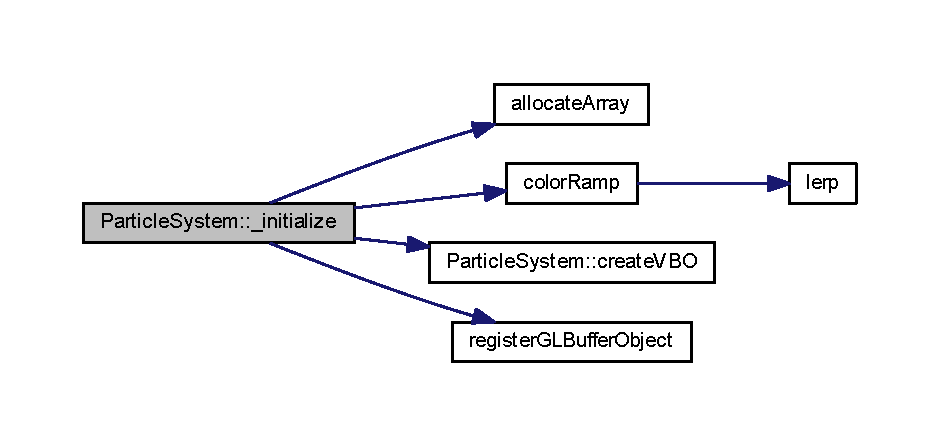
\includegraphics[width=350pt]{class_particle_system_a484988642e046424d32a13709204e8de_cgraph}
\end{center}
\end{figure}




Oto graf wywoływań tej funkcji\-:\nopagebreak
\begin{figure}[H]
\begin{center}
\leavevmode
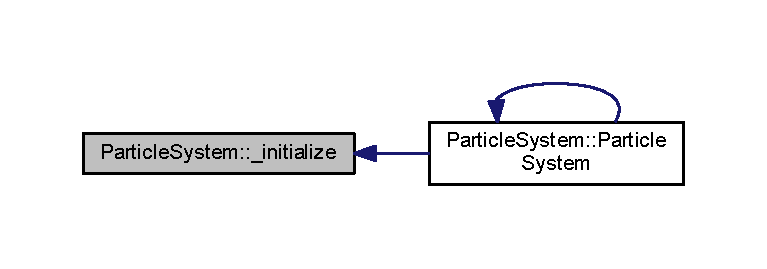
\includegraphics[width=350pt]{class_particle_system_a484988642e046424d32a13709204e8de_icgraph}
\end{center}
\end{figure}


\hypertarget{class_particle_system_af2f16676fe8a0523cfb867a9a856970c}{\index{Particle\-System@{Particle\-System}!add\-Sphere@{add\-Sphere}}
\index{add\-Sphere@{add\-Sphere}!ParticleSystem@{Particle\-System}}
\subsubsection[{add\-Sphere}]{\setlength{\rightskip}{0pt plus 5cm}void Particle\-System\-::add\-Sphere (
\begin{DoxyParamCaption}
\item[{int}]{index, }
\item[{float $\ast$}]{pos, }
\item[{float $\ast$}]{vel, }
\item[{int}]{r, }
\item[{float}]{spacing}
\end{DoxyParamCaption}
)}}\label{class_particle_system_af2f16676fe8a0523cfb867a9a856970c}


Definicja w linii \hyperlink{particle_system_8cpp_source_l00485}{485} pliku \hyperlink{particle_system_8cpp_source}{particle\-System.\-cpp}.



Odwołuje się do \hyperlink{particle_system_8h_source_l00156}{m\-\_\-h\-Pos}, \hyperlink{particle_system_8h_source_l00157}{m\-\_\-h\-Vel}, \hyperlink{particle_system_8h_source_l00038}{P\-O\-S\-I\-T\-I\-O\-N}, \hyperlink{particle_system_8cpp_source_l00374}{set\-Array()} i \hyperlink{particle_system_8h_source_l00039}{V\-E\-L\-O\-C\-I\-T\-Y}.



Odwołania w \hyperlink{particles_8cpp_source_l00335}{add\-Sphere()} i \hyperlink{particles_8cpp_source_l00520}{key()}.


\begin{DoxyCode}
00486 \{
00487     \hyperlink{particles__kernel_8cuh_a91ad9478d81a7aaf2593e8d9c3d06a14}{uint} index = start;
00488 
00489     \textcolor{keywordflow}{for} (\textcolor{keywordtype}{int} z=-r; z<=r; z++)
00490     \{
00491         \textcolor{keywordflow}{for} (\textcolor{keywordtype}{int} y=-r; y<=r; y++)
00492         \{
00493             \textcolor{keywordflow}{for} (\textcolor{keywordtype}{int} x=-r; x<=r; x++)
00494             \{
00495                 \textcolor{keywordtype}{float} dx = x*spacing;
00496                 \textcolor{keywordtype}{float} dy = y*spacing;
00497                 \textcolor{keywordtype}{float} dz = z*spacing;
00498                 \textcolor{keywordtype}{float} l = sqrtf(dx*dx + dy*dy + dz*dz);
00499                 \textcolor{keywordtype}{float} jitter = \hyperlink{class_particle_system_ab765472aed6a1b5f0d2f98a3a906c417}{m\_params}.\hyperlink{struct_sim_params_a7e131c24e1020c44173deb0f57a8c4af}{particleRadius}*0.01f;
00500 
00501                 \textcolor{keywordflow}{if} ((l <= \hyperlink{class_particle_system_ab765472aed6a1b5f0d2f98a3a906c417}{m\_params}.\hyperlink{struct_sim_params_a7e131c24e1020c44173deb0f57a8c4af}{particleRadius}*2.0f*r) && (index < 
      \hyperlink{class_particle_system_a23d238efa80a647d4b6cde034f486a91}{m\_numParticles}))
00502                 \{
00503                     \hyperlink{class_particle_system_ab9d75471d2eaaeb8fa98d2f3f47d9c25}{m\_hPos}[index*4]   = pos[0] + dx + (\hyperlink{particle_system_8cpp_a5459f6b6b39f9a6b80de7f17c3777ee2}{frand}()*2.0f-1.0f)*jitter;
00504                     \hyperlink{class_particle_system_ab9d75471d2eaaeb8fa98d2f3f47d9c25}{m\_hPos}[index*4+1] = pos[1] + dy + (\hyperlink{particle_system_8cpp_a5459f6b6b39f9a6b80de7f17c3777ee2}{frand}()*2.0f-1.0f)*jitter;
00505                     m\_hPos[index*4+2] = pos[2] + dz + (\hyperlink{particle_system_8cpp_a5459f6b6b39f9a6b80de7f17c3777ee2}{frand}()*2.0f-1.0f)*jitter;
00506                     m\_hPos[index*4+3] = pos[3];
00507 
00508                     \hyperlink{class_particle_system_a20560c896ee8a8bbc827a8e5902da7e2}{m\_hVel}[index*4]   = vel[0];
00509                     \hyperlink{class_particle_system_a20560c896ee8a8bbc827a8e5902da7e2}{m\_hVel}[index*4+1] = vel[1];
00510                     \hyperlink{class_particle_system_a20560c896ee8a8bbc827a8e5902da7e2}{m\_hVel}[index*4+2] = vel[2];
00511                     \hyperlink{class_particle_system_a20560c896ee8a8bbc827a8e5902da7e2}{m\_hVel}[index*4+3] = vel[3];
00512                     index++;
00513                 \}
00514             \}
00515         \}
00516     \}
00517 
00518     \hyperlink{class_particle_system_aa792a66680e800832059854aab0d594d}{setArray}(\hyperlink{class_particle_system_a332fbe57a36aaea5c18b4ea4fba6bbb3a9e9a2992d230a2674debf26e0e8e0299}{POSITION}, \hyperlink{class_particle_system_ab9d75471d2eaaeb8fa98d2f3f47d9c25}{m\_hPos}, start, index);
00519     \hyperlink{class_particle_system_aa792a66680e800832059854aab0d594d}{setArray}(\hyperlink{class_particle_system_a332fbe57a36aaea5c18b4ea4fba6bbb3a3702de73065f01b4f6ffa604b799e53d}{VELOCITY}, \hyperlink{class_particle_system_a20560c896ee8a8bbc827a8e5902da7e2}{m\_hVel}, start, index);
00520 \}
\end{DoxyCode}


Oto graf wywołań dla tej funkcji\-:\nopagebreak
\begin{figure}[H]
\begin{center}
\leavevmode
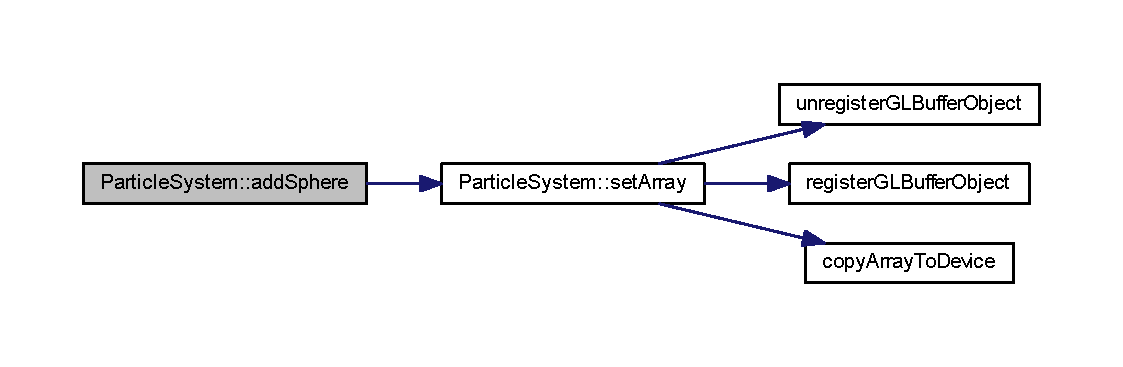
\includegraphics[width=350pt]{class_particle_system_af2f16676fe8a0523cfb867a9a856970c_cgraph}
\end{center}
\end{figure}




Oto graf wywoływań tej funkcji\-:\nopagebreak
\begin{figure}[H]
\begin{center}
\leavevmode
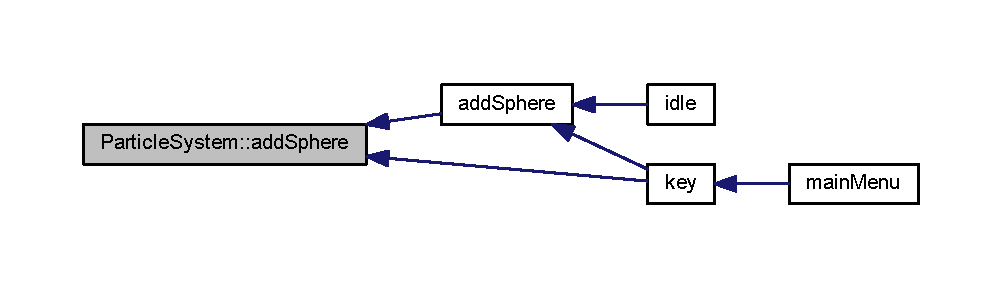
\includegraphics[width=350pt]{class_particle_system_af2f16676fe8a0523cfb867a9a856970c_icgraph}
\end{center}
\end{figure}


\hypertarget{class_particle_system_a399eb5cb9c422fd3370899e4d8a5d62e}{\index{Particle\-System@{Particle\-System}!create\-V\-B\-O@{create\-V\-B\-O}}
\index{create\-V\-B\-O@{create\-V\-B\-O}!ParticleSystem@{Particle\-System}}
\subsubsection[{create\-V\-B\-O}]{\setlength{\rightskip}{0pt plus 5cm}{\bf uint} Particle\-System\-::create\-V\-B\-O (
\begin{DoxyParamCaption}
\item[{{\bf uint}}]{size}
\end{DoxyParamCaption}
)\hspace{0.3cm}{\ttfamily [protected]}}}\label{class_particle_system_a399eb5cb9c422fd3370899e4d8a5d62e}


Definicja w linii \hyperlink{particle_system_8cpp_source_l00085}{85} pliku \hyperlink{particle_system_8cpp_source}{particle\-System.\-cpp}.



Odwołania w \hyperlink{particle_system_8cpp_source_l00123}{\-\_\-initialize()}.


\begin{DoxyCode}
00086 \{
00087     GLuint vbo;
00088     glGenBuffers(1, &vbo);
00089     glBindBuffer(GL\_ARRAY\_BUFFER, vbo);
00090     glBufferData(GL\_ARRAY\_BUFFER, size, 0, GL\_DYNAMIC\_DRAW);
00091     glBindBuffer(GL\_ARRAY\_BUFFER, 0);
00092     \textcolor{keywordflow}{return} vbo;
00093 \}
\end{DoxyCode}


Oto graf wywoływań tej funkcji\-:\nopagebreak
\begin{figure}[H]
\begin{center}
\leavevmode
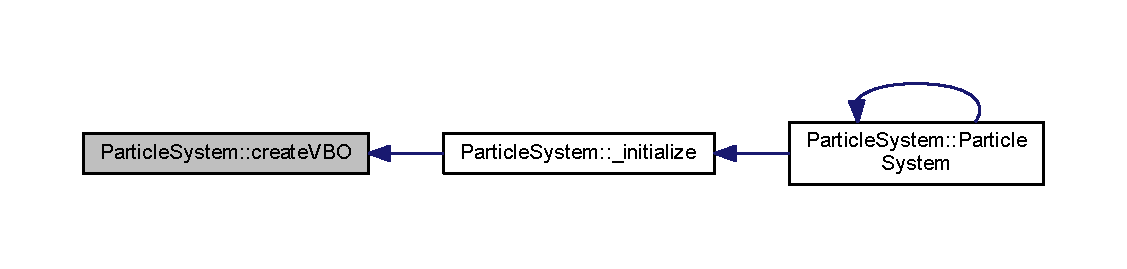
\includegraphics[width=350pt]{class_particle_system_a399eb5cb9c422fd3370899e4d8a5d62e_icgraph}
\end{center}
\end{figure}


\hypertarget{class_particle_system_a722bdb7cc940f052400a69fe9569a49e}{\index{Particle\-System@{Particle\-System}!dump\-Grid@{dump\-Grid}}
\index{dump\-Grid@{dump\-Grid}!ParticleSystem@{Particle\-System}}
\subsubsection[{dump\-Grid}]{\setlength{\rightskip}{0pt plus 5cm}void Particle\-System\-::dump\-Grid (
\begin{DoxyParamCaption}
{}
\end{DoxyParamCaption}
)}}\label{class_particle_system_a722bdb7cc940f052400a69fe9569a49e}


Definicja w linii \hyperlink{particle_system_8cpp_source_l00306}{306} pliku \hyperlink{particle_system_8cpp_source}{particle\-System.\-cpp}.



Odwołuje się do \hyperlink{particle_system__cuda_8cu_source_l00108}{copy\-Array\-From\-Device()}, \hyperlink{particle_system_8h_source_l00174}{m\-\_\-d\-Cell\-End}, \hyperlink{particle_system_8h_source_l00173}{m\-\_\-d\-Cell\-Start}, \hyperlink{particle_system_8h_source_l00161}{m\-\_\-h\-Cell\-End}, \hyperlink{particle_system_8h_source_l00160}{m\-\_\-h\-Cell\-Start} i \hyperlink{particle_system_8h_source_l00190}{m\-\_\-num\-Grid\-Cells}.



Odwołania w \hyperlink{particles_8cpp_source_l00520}{key()}.


\begin{DoxyCode}
00307 \{
00308     \textcolor{comment}{// dump grid information}
00309     \hyperlink{particles_8cpp_afed059fa8ae6691333d263c5c88281f6}{copyArrayFromDevice}(\hyperlink{class_particle_system_a8412ecd991c14d906fcebba42bdeffd3}{m\_hCellStart}, 
      \hyperlink{class_particle_system_a137909a8b34f7a42e50cd0fcc86bb784}{m\_dCellStart}, 0, \textcolor{keyword}{sizeof}(\hyperlink{particles__kernel_8cuh_a91ad9478d81a7aaf2593e8d9c3d06a14}{uint})*\hyperlink{class_particle_system_aa1ef17d723af5d7a4685e8fd57e9ca89}{m\_numGridCells});
00310     \hyperlink{particles_8cpp_afed059fa8ae6691333d263c5c88281f6}{copyArrayFromDevice}(\hyperlink{class_particle_system_a8d8ad2d142f3a5b83f2c10a46f5d7a8b}{m\_hCellEnd}, \hyperlink{class_particle_system_a3a0b9c760c2bfcf811d54b8194ebea01}{m\_dCellEnd}, 0, \textcolor{keyword}{sizeof}(
      \hyperlink{particles__kernel_8cuh_a91ad9478d81a7aaf2593e8d9c3d06a14}{uint})*\hyperlink{class_particle_system_aa1ef17d723af5d7a4685e8fd57e9ca89}{m\_numGridCells});
00311     \hyperlink{particles__kernel_8cuh_a91ad9478d81a7aaf2593e8d9c3d06a14}{uint} maxCellSize = 0;
00312 
00313     \textcolor{keywordflow}{for} (\hyperlink{particles__kernel_8cuh_a91ad9478d81a7aaf2593e8d9c3d06a14}{uint} i=0; i<\hyperlink{class_particle_system_aa1ef17d723af5d7a4685e8fd57e9ca89}{m\_numGridCells}; i++)
00314     \{
00315         \textcolor{keywordflow}{if} (\hyperlink{class_particle_system_a8412ecd991c14d906fcebba42bdeffd3}{m\_hCellStart}[i] != 0xffffffff)
00316         \{
00317             \hyperlink{particles__kernel_8cuh_a91ad9478d81a7aaf2593e8d9c3d06a14}{uint} cellSize = \hyperlink{class_particle_system_a8d8ad2d142f3a5b83f2c10a46f5d7a8b}{m\_hCellEnd}[i] - \hyperlink{class_particle_system_a8412ecd991c14d906fcebba42bdeffd3}{m\_hCellStart}[i];
00318 
00319             \textcolor{comment}{//            printf("cell: %d, %d particles\(\backslash\)n", i, cellSize);}
00320             \textcolor{keywordflow}{if} (cellSize > maxCellSize)
00321             \{
00322                 maxCellSize = cellSize;
00323             \}
00324         \}
00325     \}
00326 
00327     printf(\textcolor{stringliteral}{"maximum particles per cell = %d\(\backslash\)n"}, maxCellSize);
00328 \}
\end{DoxyCode}


Oto graf wywołań dla tej funkcji\-:\nopagebreak
\begin{figure}[H]
\begin{center}
\leavevmode
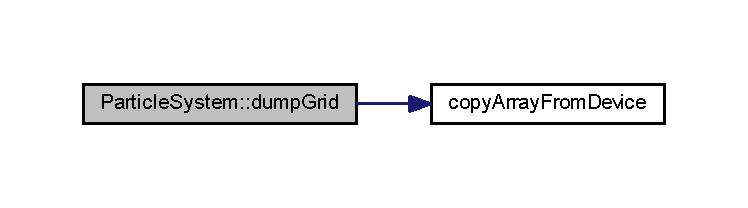
\includegraphics[width=350pt]{class_particle_system_a722bdb7cc940f052400a69fe9569a49e_cgraph}
\end{center}
\end{figure}




Oto graf wywoływań tej funkcji\-:\nopagebreak
\begin{figure}[H]
\begin{center}
\leavevmode
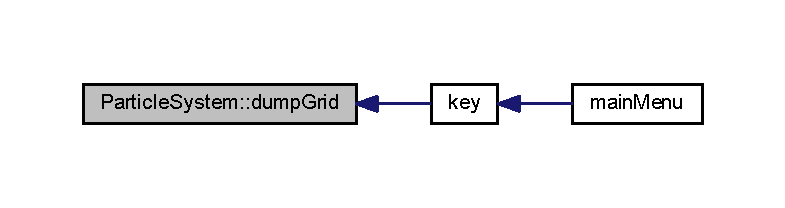
\includegraphics[width=350pt]{class_particle_system_a722bdb7cc940f052400a69fe9569a49e_icgraph}
\end{center}
\end{figure}


\hypertarget{class_particle_system_a9025f319e07c58c6ece1cd2a620ce33a}{\index{Particle\-System@{Particle\-System}!dump\-Particles@{dump\-Particles}}
\index{dump\-Particles@{dump\-Particles}!ParticleSystem@{Particle\-System}}
\subsubsection[{dump\-Particles}]{\setlength{\rightskip}{0pt plus 5cm}void Particle\-System\-::dump\-Particles (
\begin{DoxyParamCaption}
\item[{{\bf uint}}]{start, }
\item[{{\bf uint}}]{count}
\end{DoxyParamCaption}
)}}\label{class_particle_system_a9025f319e07c58c6ece1cd2a620ce33a}


Definicja w linii \hyperlink{particle_system_8cpp_source_l00331}{331} pliku \hyperlink{particle_system_8cpp_source}{particle\-System.\-cpp}.



Odwołuje się do \hyperlink{particle_system__cuda_8cu_source_l00108}{copy\-Array\-From\-Device()}, \hyperlink{particle_system_8h_source_l00184}{m\-\_\-cuda\-\_\-posvbo\-\_\-resource}, \hyperlink{particle_system_8h_source_l00165}{m\-\_\-d\-Vel}, \hyperlink{particle_system_8h_source_l00156}{m\-\_\-h\-Pos} i \hyperlink{particle_system_8h_source_l00157}{m\-\_\-h\-Vel}.



Odwołania w \hyperlink{particles_8cpp_source_l00520}{key()}.


\begin{DoxyCode}
00332 \{
00333     \textcolor{comment}{// debug}
00334     \hyperlink{particles_8cpp_afed059fa8ae6691333d263c5c88281f6}{copyArrayFromDevice}(\hyperlink{class_particle_system_ab9d75471d2eaaeb8fa98d2f3f47d9c25}{m\_hPos}, 0, &
      \hyperlink{class_particle_system_a9c5de70c1705672e5722ad30dee1b14b}{m\_cuda\_posvbo\_resource}, \textcolor{keyword}{sizeof}(\textcolor{keywordtype}{float})*4*count);
00335     \hyperlink{particles_8cpp_afed059fa8ae6691333d263c5c88281f6}{copyArrayFromDevice}(\hyperlink{class_particle_system_a20560c896ee8a8bbc827a8e5902da7e2}{m\_hVel}, \hyperlink{class_particle_system_a5efd31a2fdba8d98b105f4e546964cb5}{m\_dVel}, 0, \textcolor{keyword}{sizeof}(\textcolor{keywordtype}{float})*4*count);
00336 
00337     \textcolor{keywordflow}{for} (\hyperlink{particles__kernel_8cuh_a91ad9478d81a7aaf2593e8d9c3d06a14}{uint} i=start; i<start+count; i++)
00338     \{
00339         \textcolor{comment}{//        printf("%d: ", i);}
00340         printf(\textcolor{stringliteral}{"pos: (%.4f, %.4f, %.4f, %.4f)\(\backslash\)n"}, \hyperlink{class_particle_system_ab9d75471d2eaaeb8fa98d2f3f47d9c25}{m\_hPos}[i*4+0], \hyperlink{class_particle_system_ab9d75471d2eaaeb8fa98d2f3f47d9c25}{m\_hPos}[i*4+1], 
      \hyperlink{class_particle_system_ab9d75471d2eaaeb8fa98d2f3f47d9c25}{m\_hPos}[i*4+2], \hyperlink{class_particle_system_ab9d75471d2eaaeb8fa98d2f3f47d9c25}{m\_hPos}[i*4+3]);
00341         printf(\textcolor{stringliteral}{"vel: (%.4f, %.4f, %.4f, %.4f)\(\backslash\)n"}, \hyperlink{class_particle_system_a20560c896ee8a8bbc827a8e5902da7e2}{m\_hVel}[i*4+0], \hyperlink{class_particle_system_a20560c896ee8a8bbc827a8e5902da7e2}{m\_hVel}[i*4+1], 
      \hyperlink{class_particle_system_a20560c896ee8a8bbc827a8e5902da7e2}{m\_hVel}[i*4+2], \hyperlink{class_particle_system_a20560c896ee8a8bbc827a8e5902da7e2}{m\_hVel}[i*4+3]);
00342     \}
00343 \}
\end{DoxyCode}


Oto graf wywołań dla tej funkcji\-:\nopagebreak
\begin{figure}[H]
\begin{center}
\leavevmode
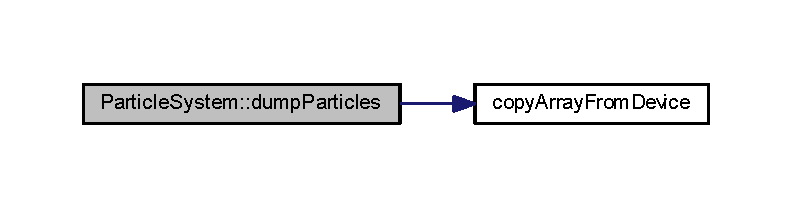
\includegraphics[width=350pt]{class_particle_system_a9025f319e07c58c6ece1cd2a620ce33a_cgraph}
\end{center}
\end{figure}




Oto graf wywoływań tej funkcji\-:\nopagebreak
\begin{figure}[H]
\begin{center}
\leavevmode
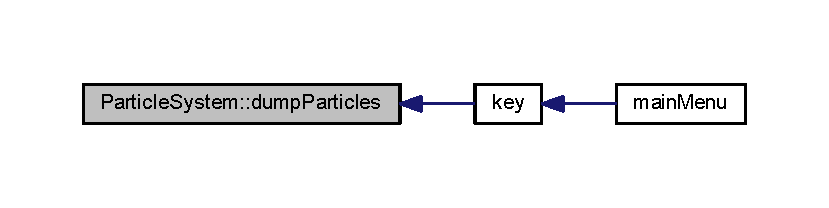
\includegraphics[width=350pt]{class_particle_system_a9025f319e07c58c6ece1cd2a620ce33a_icgraph}
\end{center}
\end{figure}


\hypertarget{class_particle_system_a8bdfaa6198651ef0ceb8be489ecd78e3}{\index{Particle\-System@{Particle\-System}!get\-Array@{get\-Array}}
\index{get\-Array@{get\-Array}!ParticleSystem@{Particle\-System}}
\subsubsection[{get\-Array}]{\setlength{\rightskip}{0pt plus 5cm}float $\ast$ Particle\-System\-::get\-Array (
\begin{DoxyParamCaption}
\item[{{\bf Particle\-Array}}]{array}
\end{DoxyParamCaption}
)}}\label{class_particle_system_a8bdfaa6198651ef0ceb8be489ecd78e3}


Definicja w linii \hyperlink{particle_system_8cpp_source_l00346}{346} pliku \hyperlink{particle_system_8cpp_source}{particle\-System.\-cpp}.



Odwołuje się do \hyperlink{particle_system__cuda_8cu_source_l00108}{copy\-Array\-From\-Device()}, \hyperlink{particle_system_8h_source_l00152}{m\-\_\-b\-Initialized}, \hyperlink{particle_system_8h_source_l00184}{m\-\_\-cuda\-\_\-posvbo\-\_\-resource}, \hyperlink{particle_system_8h_source_l00164}{m\-\_\-d\-Pos}, \hyperlink{particle_system_8h_source_l00165}{m\-\_\-d\-Vel}, \hyperlink{particle_system_8h_source_l00156}{m\-\_\-h\-Pos}, \hyperlink{particle_system_8h_source_l00157}{m\-\_\-h\-Vel}, \hyperlink{particle_system_8h_source_l00153}{m\-\_\-num\-Particles}, \hyperlink{particle_system_8h_source_l00038}{P\-O\-S\-I\-T\-I\-O\-N} i \hyperlink{particle_system_8h_source_l00039}{V\-E\-L\-O\-C\-I\-T\-Y}.


\begin{DoxyCode}
00347 \{
00348     assert(\hyperlink{class_particle_system_a21bbfba9d8701a70bc6fddbf4fc3f5bd}{m\_bInitialized});
00349 
00350     \textcolor{keywordtype}{float} *hdata = 0;
00351     \textcolor{keywordtype}{float} *ddata = 0;
00352     \textcolor{keyword}{struct }cudaGraphicsResource *cuda\_vbo\_resource = 0;
00353 
00354     \textcolor{keywordflow}{switch} (array)
00355     \{
00356         \textcolor{keywordflow}{default}:
00357         \textcolor{keywordflow}{case} \hyperlink{class_particle_system_a332fbe57a36aaea5c18b4ea4fba6bbb3a9e9a2992d230a2674debf26e0e8e0299}{POSITION}:
00358             hdata = \hyperlink{class_particle_system_ab9d75471d2eaaeb8fa98d2f3f47d9c25}{m\_hPos};
00359             ddata = \hyperlink{class_particle_system_afff6217d2726217dff77c81ef3c23bfa}{m\_dPos};
00360             cuda\_vbo\_resource = \hyperlink{class_particle_system_a9c5de70c1705672e5722ad30dee1b14b}{m\_cuda\_posvbo\_resource};
00361             \textcolor{keywordflow}{break};
00362 
00363         \textcolor{keywordflow}{case} \hyperlink{class_particle_system_a332fbe57a36aaea5c18b4ea4fba6bbb3a3702de73065f01b4f6ffa604b799e53d}{VELOCITY}:
00364             hdata = \hyperlink{class_particle_system_a20560c896ee8a8bbc827a8e5902da7e2}{m\_hVel};
00365             ddata = \hyperlink{class_particle_system_a5efd31a2fdba8d98b105f4e546964cb5}{m\_dVel};
00366             \textcolor{keywordflow}{break};
00367     \}
00368 
00369     \hyperlink{particles_8cpp_afed059fa8ae6691333d263c5c88281f6}{copyArrayFromDevice}(hdata, ddata, &cuda\_vbo\_resource, 
      \hyperlink{class_particle_system_a23d238efa80a647d4b6cde034f486a91}{m\_numParticles}*4*\textcolor{keyword}{sizeof}(\textcolor{keywordtype}{float}));
00370     \textcolor{keywordflow}{return} hdata;
00371 \}
\end{DoxyCode}


Oto graf wywołań dla tej funkcji\-:\nopagebreak
\begin{figure}[H]
\begin{center}
\leavevmode
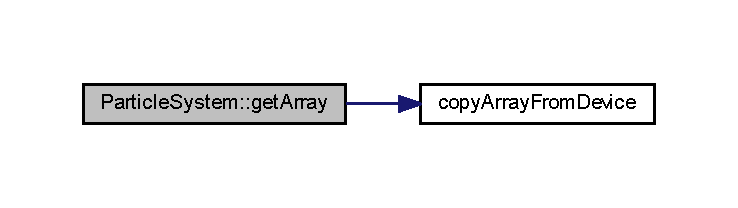
\includegraphics[width=350pt]{class_particle_system_a8bdfaa6198651ef0ceb8be489ecd78e3_cgraph}
\end{center}
\end{figure}


\hypertarget{class_particle_system_a608bcb87f3d30fbfeae810da28ae1052}{\index{Particle\-System@{Particle\-System}!get\-Cell\-Size@{get\-Cell\-Size}}
\index{get\-Cell\-Size@{get\-Cell\-Size}!ParticleSystem@{Particle\-System}}
\subsubsection[{get\-Cell\-Size}]{\setlength{\rightskip}{0pt plus 5cm}float3 Particle\-System\-::get\-Cell\-Size (
\begin{DoxyParamCaption}
{}
\end{DoxyParamCaption}
)\hspace{0.3cm}{\ttfamily [inline]}}}\label{class_particle_system_a608bcb87f3d30fbfeae810da28ae1052}


Definicja w linii \hyperlink{particle_system_8h_source_l00135}{135} pliku \hyperlink{particle_system_8h_source}{particle\-System.\-h}.


\begin{DoxyCode}
00136         \{
00137             \textcolor{keywordflow}{return} \hyperlink{class_particle_system_ab765472aed6a1b5f0d2f98a3a906c417}{m\_params}.\hyperlink{struct_sim_params_ad5d71ad4ba6acc829a35f47b3da3e169}{cellSize};
00138         \}
\end{DoxyCode}
\hypertarget{class_particle_system_a3c8578d474f5a6f14d903a242aec96ec}{\index{Particle\-System@{Particle\-System}!get\-Collider\-Pos@{get\-Collider\-Pos}}
\index{get\-Collider\-Pos@{get\-Collider\-Pos}!ParticleSystem@{Particle\-System}}
\subsubsection[{get\-Collider\-Pos}]{\setlength{\rightskip}{0pt plus 5cm}float3 Particle\-System\-::get\-Collider\-Pos (
\begin{DoxyParamCaption}
{}
\end{DoxyParamCaption}
)\hspace{0.3cm}{\ttfamily [inline]}}}\label{class_particle_system_a3c8578d474f5a6f14d903a242aec96ec}


Definicja w linii \hyperlink{particle_system_8h_source_l00119}{119} pliku \hyperlink{particle_system_8h_source}{particle\-System.\-h}.


\begin{DoxyCode}
00120         \{
00121             \textcolor{keywordflow}{return} \hyperlink{class_particle_system_ab765472aed6a1b5f0d2f98a3a906c417}{m\_params}.\hyperlink{struct_sim_params_aa27be265020f137f0a9cfbc3f1d2d9f8}{colliderPos};
00122         \}
\end{DoxyCode}
\hypertarget{class_particle_system_a56f07dfab9d5cbf510c6e0a28e816038}{\index{Particle\-System@{Particle\-System}!get\-Collider\-Radius@{get\-Collider\-Radius}}
\index{get\-Collider\-Radius@{get\-Collider\-Radius}!ParticleSystem@{Particle\-System}}
\subsubsection[{get\-Collider\-Radius}]{\setlength{\rightskip}{0pt plus 5cm}float Particle\-System\-::get\-Collider\-Radius (
\begin{DoxyParamCaption}
{}
\end{DoxyParamCaption}
)\hspace{0.3cm}{\ttfamily [inline]}}}\label{class_particle_system_a56f07dfab9d5cbf510c6e0a28e816038}


Definicja w linii \hyperlink{particle_system_8h_source_l00123}{123} pliku \hyperlink{particle_system_8h_source}{particle\-System.\-h}.


\begin{DoxyCode}
00124         \{
00125             \textcolor{keywordflow}{return} \hyperlink{class_particle_system_ab765472aed6a1b5f0d2f98a3a906c417}{m\_params}.\hyperlink{struct_sim_params_a06ca2162f6f0aec08343db6ed8cd4478}{colliderRadius};
00126         \}
\end{DoxyCode}
\hypertarget{class_particle_system_a5d300a37ebf1a2fb8575f82ced6a208f}{\index{Particle\-System@{Particle\-System}!get\-Color\-Buffer@{get\-Color\-Buffer}}
\index{get\-Color\-Buffer@{get\-Color\-Buffer}!ParticleSystem@{Particle\-System}}
\subsubsection[{get\-Color\-Buffer}]{\setlength{\rightskip}{0pt plus 5cm}unsigned int Particle\-System\-::get\-Color\-Buffer (
\begin{DoxyParamCaption}
{}
\end{DoxyParamCaption}
) const\hspace{0.3cm}{\ttfamily [inline]}}}\label{class_particle_system_a5d300a37ebf1a2fb8575f82ced6a208f}


Definicja w linii \hyperlink{particle_system_8h_source_l00057}{57} pliku \hyperlink{particle_system_8h_source}{particle\-System.\-h}.



Odwołuje się do \hyperlink{particle_system_8h_source_l00179}{m\-\_\-color\-V\-B\-O}.



Odwołania w \hyperlink{particles_8cpp_source_l00142}{init\-Particle\-System()}.


\begin{DoxyCode}
00058         \{
00059             \textcolor{keywordflow}{return} \hyperlink{class_particle_system_a96b05c719006c9e3eaed759f54a49c7f}{m\_colorVBO};
00060         \}
\end{DoxyCode}


Oto graf wywoływań tej funkcji\-:\nopagebreak
\begin{figure}[H]
\begin{center}
\leavevmode
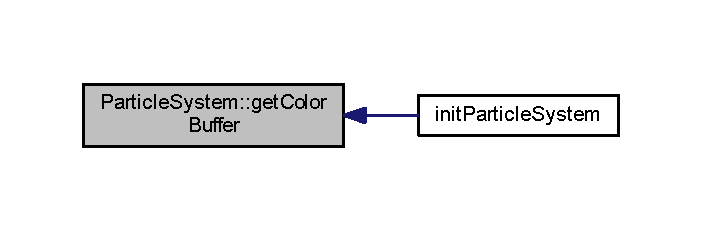
\includegraphics[width=337pt]{class_particle_system_a5d300a37ebf1a2fb8575f82ced6a208f_icgraph}
\end{center}
\end{figure}


\hypertarget{class_particle_system_af89375a9131276f941dccefa7840adda}{\index{Particle\-System@{Particle\-System}!get\-Cuda\-Color\-V\-B\-O@{get\-Cuda\-Color\-V\-B\-O}}
\index{get\-Cuda\-Color\-V\-B\-O@{get\-Cuda\-Color\-V\-B\-O}!ParticleSystem@{Particle\-System}}
\subsubsection[{get\-Cuda\-Color\-V\-B\-O}]{\setlength{\rightskip}{0pt plus 5cm}void$\ast$ Particle\-System\-::get\-Cuda\-Color\-V\-B\-O (
\begin{DoxyParamCaption}
{}
\end{DoxyParamCaption}
) const\hspace{0.3cm}{\ttfamily [inline]}}}\label{class_particle_system_af89375a9131276f941dccefa7840adda}


Definicja w linii \hyperlink{particle_system_8h_source_l00066}{66} pliku \hyperlink{particle_system_8h_source}{particle\-System.\-h}.



Odwołuje się do \hyperlink{particle_system_8h_source_l00182}{m\-\_\-cuda\-Color\-V\-B\-O}.


\begin{DoxyCode}
00067         \{
00068             \textcolor{keywordflow}{return} (\textcolor{keywordtype}{void} *)\hyperlink{class_particle_system_a39d210b57da5f7f4a2c23f4fc0b43ea1}{m\_cudaColorVBO};
00069         \}
\end{DoxyCode}
\hypertarget{class_particle_system_a2c8214a5bcd9d9c24d16e1f0063c06d6}{\index{Particle\-System@{Particle\-System}!get\-Cuda\-Pos\-V\-B\-O@{get\-Cuda\-Pos\-V\-B\-O}}
\index{get\-Cuda\-Pos\-V\-B\-O@{get\-Cuda\-Pos\-V\-B\-O}!ParticleSystem@{Particle\-System}}
\subsubsection[{get\-Cuda\-Pos\-V\-B\-O}]{\setlength{\rightskip}{0pt plus 5cm}void$\ast$ Particle\-System\-::get\-Cuda\-Pos\-V\-B\-O (
\begin{DoxyParamCaption}
{}
\end{DoxyParamCaption}
) const\hspace{0.3cm}{\ttfamily [inline]}}}\label{class_particle_system_a2c8214a5bcd9d9c24d16e1f0063c06d6}


Definicja w linii \hyperlink{particle_system_8h_source_l00062}{62} pliku \hyperlink{particle_system_8h_source}{particle\-System.\-h}.



Odwołuje się do \hyperlink{particle_system_8h_source_l00181}{m\-\_\-cuda\-Pos\-V\-B\-O}.



Odwołania w \hyperlink{particles_8cpp_source_l00194}{run\-Benchmark()}.


\begin{DoxyCode}
00063         \{
00064             \textcolor{keywordflow}{return} (\textcolor{keywordtype}{void} *)\hyperlink{class_particle_system_aba18245745f621d90186862f1a559d9e}{m\_cudaPosVBO};
00065         \}
\end{DoxyCode}


Oto graf wywoływań tej funkcji\-:\nopagebreak
\begin{figure}[H]
\begin{center}
\leavevmode
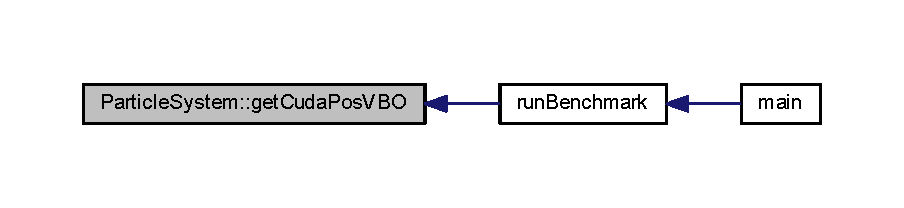
\includegraphics[width=350pt]{class_particle_system_a2c8214a5bcd9d9c24d16e1f0063c06d6_icgraph}
\end{center}
\end{figure}


\hypertarget{class_particle_system_ae9f149d6b7c3b148fc397473c7c3c2e2}{\index{Particle\-System@{Particle\-System}!get\-Current\-Read\-Buffer@{get\-Current\-Read\-Buffer}}
\index{get\-Current\-Read\-Buffer@{get\-Current\-Read\-Buffer}!ParticleSystem@{Particle\-System}}
\subsubsection[{get\-Current\-Read\-Buffer}]{\setlength{\rightskip}{0pt plus 5cm}unsigned int Particle\-System\-::get\-Current\-Read\-Buffer (
\begin{DoxyParamCaption}
{}
\end{DoxyParamCaption}
) const\hspace{0.3cm}{\ttfamily [inline]}}}\label{class_particle_system_ae9f149d6b7c3b148fc397473c7c3c2e2}


Definicja w linii \hyperlink{particle_system_8h_source_l00053}{53} pliku \hyperlink{particle_system_8h_source}{particle\-System.\-h}.



Odwołuje się do \hyperlink{particle_system_8h_source_l00178}{m\-\_\-pos\-Vbo}.



Odwołania w \hyperlink{particles_8cpp_source_l00248}{display()} i \hyperlink{particles_8cpp_source_l00520}{key()}.


\begin{DoxyCode}
00054         \{
00055             \textcolor{keywordflow}{return} \hyperlink{class_particle_system_a31f9cccdf5dbae6f72867665bd8761e3}{m\_posVbo};
00056         \}
\end{DoxyCode}


Oto graf wywoływań tej funkcji\-:\nopagebreak
\begin{figure}[H]
\begin{center}
\leavevmode
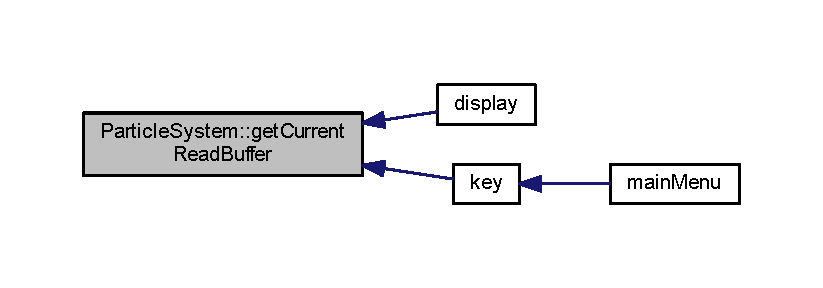
\includegraphics[width=350pt]{class_particle_system_ae9f149d6b7c3b148fc397473c7c3c2e2_icgraph}
\end{center}
\end{figure}


\hypertarget{class_particle_system_af94ba180bcb348afcfd81bb699d6aab0}{\index{Particle\-System@{Particle\-System}!get\-Grid\-Size@{get\-Grid\-Size}}
\index{get\-Grid\-Size@{get\-Grid\-Size}!ParticleSystem@{Particle\-System}}
\subsubsection[{get\-Grid\-Size}]{\setlength{\rightskip}{0pt plus 5cm}uint3 Particle\-System\-::get\-Grid\-Size (
\begin{DoxyParamCaption}
{}
\end{DoxyParamCaption}
)\hspace{0.3cm}{\ttfamily [inline]}}}\label{class_particle_system_af94ba180bcb348afcfd81bb699d6aab0}


Definicja w linii \hyperlink{particle_system_8h_source_l00127}{127} pliku \hyperlink{particle_system_8h_source}{particle\-System.\-h}.


\begin{DoxyCode}
00128         \{
00129             \textcolor{keywordflow}{return} \hyperlink{class_particle_system_ab765472aed6a1b5f0d2f98a3a906c417}{m\_params}.\hyperlink{struct_sim_params_a4cfb18ff777876da3ad69aae6e023949}{gridSize};
00130         \}
\end{DoxyCode}
\hypertarget{class_particle_system_a6f89e8d4c3e3e328088b7d652cee84b0}{\index{Particle\-System@{Particle\-System}!get\-Num\-Particles@{get\-Num\-Particles}}
\index{get\-Num\-Particles@{get\-Num\-Particles}!ParticleSystem@{Particle\-System}}
\subsubsection[{get\-Num\-Particles}]{\setlength{\rightskip}{0pt plus 5cm}int Particle\-System\-::get\-Num\-Particles (
\begin{DoxyParamCaption}
{}
\end{DoxyParamCaption}
) const\hspace{0.3cm}{\ttfamily [inline]}}}\label{class_particle_system_a6f89e8d4c3e3e328088b7d652cee84b0}


Definicja w linii \hyperlink{particle_system_8h_source_l00048}{48} pliku \hyperlink{particle_system_8h_source}{particle\-System.\-h}.



Odwołuje się do \hyperlink{particle_system_8h_source_l00153}{m\-\_\-num\-Particles}.



Odwołania w \hyperlink{particles_8cpp_source_l00248}{display()}, \hyperlink{particles_8cpp_source_l00520}{key()} i \hyperlink{particles_8cpp_source_l00194}{run\-Benchmark()}.


\begin{DoxyCode}
00049         \{
00050             \textcolor{keywordflow}{return} \hyperlink{class_particle_system_a23d238efa80a647d4b6cde034f486a91}{m\_numParticles};
00051         \}
\end{DoxyCode}


Oto graf wywoływań tej funkcji\-:\nopagebreak
\begin{figure}[H]
\begin{center}
\leavevmode
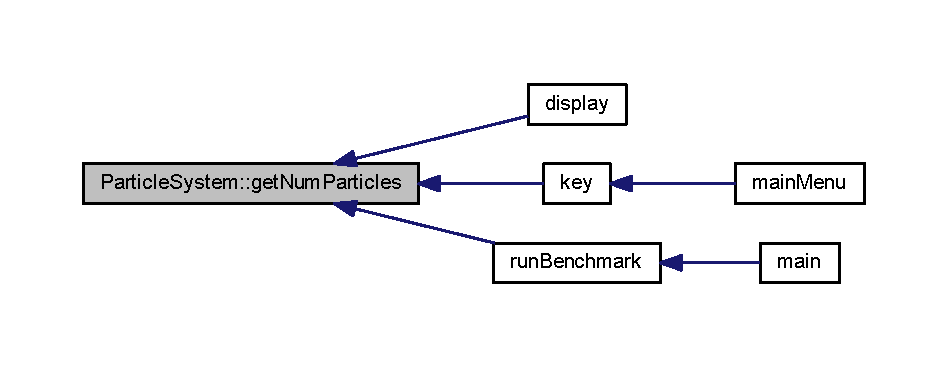
\includegraphics[width=350pt]{class_particle_system_a6f89e8d4c3e3e328088b7d652cee84b0_icgraph}
\end{center}
\end{figure}


\hypertarget{class_particle_system_abdb59a91d8483017ad71455bb2958993}{\index{Particle\-System@{Particle\-System}!get\-Particle\-Radius@{get\-Particle\-Radius}}
\index{get\-Particle\-Radius@{get\-Particle\-Radius}!ParticleSystem@{Particle\-System}}
\subsubsection[{get\-Particle\-Radius}]{\setlength{\rightskip}{0pt plus 5cm}float Particle\-System\-::get\-Particle\-Radius (
\begin{DoxyParamCaption}
{}
\end{DoxyParamCaption}
)\hspace{0.3cm}{\ttfamily [inline]}}}\label{class_particle_system_abdb59a91d8483017ad71455bb2958993}


Definicja w linii \hyperlink{particle_system_8h_source_l00115}{115} pliku \hyperlink{particle_system_8h_source}{particle\-System.\-h}.



Odwołania w \hyperlink{particles_8cpp_source_l00335}{add\-Sphere()}, \hyperlink{particles_8cpp_source_l00142}{init\-Particle\-System()} i \hyperlink{particles_8cpp_source_l00520}{key()}.


\begin{DoxyCode}
00116         \{
00117             \textcolor{keywordflow}{return} \hyperlink{class_particle_system_ab765472aed6a1b5f0d2f98a3a906c417}{m\_params}.\hyperlink{struct_sim_params_a7e131c24e1020c44173deb0f57a8c4af}{particleRadius};
00118         \}
\end{DoxyCode}


Oto graf wywoływań tej funkcji\-:\nopagebreak
\begin{figure}[H]
\begin{center}
\leavevmode
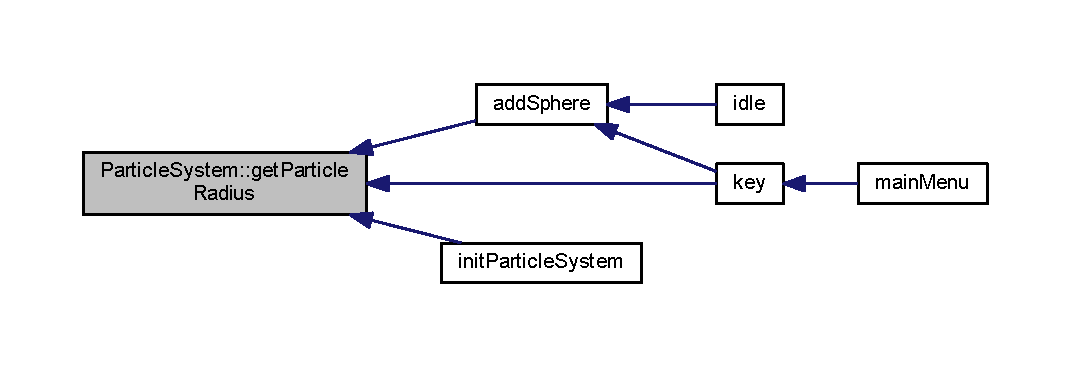
\includegraphics[width=350pt]{class_particle_system_abdb59a91d8483017ad71455bb2958993_icgraph}
\end{center}
\end{figure}


\hypertarget{class_particle_system_a19d9bb799a5b5704d8fd6a286f6be20d}{\index{Particle\-System@{Particle\-System}!get\-World\-Origin@{get\-World\-Origin}}
\index{get\-World\-Origin@{get\-World\-Origin}!ParticleSystem@{Particle\-System}}
\subsubsection[{get\-World\-Origin}]{\setlength{\rightskip}{0pt plus 5cm}float3 Particle\-System\-::get\-World\-Origin (
\begin{DoxyParamCaption}
{}
\end{DoxyParamCaption}
)\hspace{0.3cm}{\ttfamily [inline]}}}\label{class_particle_system_a19d9bb799a5b5704d8fd6a286f6be20d}


Definicja w linii \hyperlink{particle_system_8h_source_l00131}{131} pliku \hyperlink{particle_system_8h_source}{particle\-System.\-h}.


\begin{DoxyCode}
00132         \{
00133             \textcolor{keywordflow}{return} \hyperlink{class_particle_system_ab765472aed6a1b5f0d2f98a3a906c417}{m\_params}.\hyperlink{struct_sim_params_a1ed7465773f15f2874650f19cec3d0a9}{worldOrigin};
00134         \}
\end{DoxyCode}
\hypertarget{class_particle_system_a2e08c4e354b0de5e2dc468a0fb457dfe}{\index{Particle\-System@{Particle\-System}!init\-Grid@{init\-Grid}}
\index{init\-Grid@{init\-Grid}!ParticleSystem@{Particle\-System}}
\subsubsection[{init\-Grid}]{\setlength{\rightskip}{0pt plus 5cm}void Particle\-System\-::init\-Grid (
\begin{DoxyParamCaption}
\item[{{\bf uint} $\ast$}]{size, }
\item[{float}]{spacing, }
\item[{float}]{jitter, }
\item[{{\bf uint}}]{num\-Particles}
\end{DoxyParamCaption}
)\hspace{0.3cm}{\ttfamily [protected]}}}\label{class_particle_system_a2e08c4e354b0de5e2dc468a0fb457dfe}


Definicja w linii \hyperlink{particle_system_8cpp_source_l00406}{406} pliku \hyperlink{particle_system_8cpp_source}{particle\-System.\-cpp}.



Odwołuje się do \hyperlink{particle_system_8h_source_l00156}{m\-\_\-h\-Pos} i \hyperlink{particle_system_8h_source_l00157}{m\-\_\-h\-Vel}.


\begin{DoxyCode}
00407 \{
00408     srand(1973);
00409 
00410     \textcolor{keywordflow}{for} (\hyperlink{particles__kernel_8cuh_a91ad9478d81a7aaf2593e8d9c3d06a14}{uint} z=0; z<size[2]; z++)
00411     \{
00412         \textcolor{keywordflow}{for} (\hyperlink{particles__kernel_8cuh_a91ad9478d81a7aaf2593e8d9c3d06a14}{uint} y=0; y<size[1]; y++)
00413         \{
00414             \textcolor{keywordflow}{for} (\hyperlink{particles__kernel_8cuh_a91ad9478d81a7aaf2593e8d9c3d06a14}{uint} x=0; x<size[0]; x++)
00415             \{
00416                 \hyperlink{particles__kernel_8cuh_a91ad9478d81a7aaf2593e8d9c3d06a14}{uint} i = (z*size[1]*size[0]) + (y*size[0]) + x;
00417 
00418                 \textcolor{keywordflow}{if} (i < \hyperlink{particles_8cpp_a05b8a90212054a3eb1a036ae0c269596}{numParticles})
00419                 \{
00420                     \hyperlink{class_particle_system_ab9d75471d2eaaeb8fa98d2f3f47d9c25}{m\_hPos}[i*4] = (spacing * x) + \hyperlink{class_particle_system_ab765472aed6a1b5f0d2f98a3a906c417}{m\_params}.
      \hyperlink{struct_sim_params_a7e131c24e1020c44173deb0f57a8c4af}{particleRadius} - 1.0f + (\hyperlink{particle_system_8cpp_a5459f6b6b39f9a6b80de7f17c3777ee2}{frand}()*2.0f-1.0f)*jitter;
00421                     \hyperlink{class_particle_system_ab9d75471d2eaaeb8fa98d2f3f47d9c25}{m\_hPos}[i*4+1] = (spacing * y) + \hyperlink{class_particle_system_ab765472aed6a1b5f0d2f98a3a906c417}{m\_params}.
      \hyperlink{struct_sim_params_a7e131c24e1020c44173deb0f57a8c4af}{particleRadius} - 1.0f + (\hyperlink{particle_system_8cpp_a5459f6b6b39f9a6b80de7f17c3777ee2}{frand}()*2.0f-1.0f)*jitter;
00422                     \hyperlink{class_particle_system_ab9d75471d2eaaeb8fa98d2f3f47d9c25}{m\_hPos}[i*4+2] = (spacing * z) + \hyperlink{class_particle_system_ab765472aed6a1b5f0d2f98a3a906c417}{m\_params}.
      \hyperlink{struct_sim_params_a7e131c24e1020c44173deb0f57a8c4af}{particleRadius} - 1.0f + (\hyperlink{particle_system_8cpp_a5459f6b6b39f9a6b80de7f17c3777ee2}{frand}()*2.0f-1.0f)*jitter;
00423                     \hyperlink{class_particle_system_ab9d75471d2eaaeb8fa98d2f3f47d9c25}{m\_hPos}[i*4+3] = 1.0f;
00424 
00425                     \hyperlink{class_particle_system_a20560c896ee8a8bbc827a8e5902da7e2}{m\_hVel}[i*4] = 0.0f;
00426                     \hyperlink{class_particle_system_a20560c896ee8a8bbc827a8e5902da7e2}{m\_hVel}[i*4+1] = 0.0f;
00427                     \hyperlink{class_particle_system_a20560c896ee8a8bbc827a8e5902da7e2}{m\_hVel}[i*4+2] = 0.0f;
00428                     \hyperlink{class_particle_system_a20560c896ee8a8bbc827a8e5902da7e2}{m\_hVel}[i*4+3] = 0.0f;
00429                 \}
00430             \}
00431         \}
00432     \}
00433 \}
\end{DoxyCode}
\hypertarget{class_particle_system_a519070812dd9eb349f270c793c5f64b6}{\index{Particle\-System@{Particle\-System}!reset@{reset}}
\index{reset@{reset}!ParticleSystem@{Particle\-System}}
\subsubsection[{reset}]{\setlength{\rightskip}{0pt plus 5cm}void Particle\-System\-::reset (
\begin{DoxyParamCaption}
\item[{{\bf Particle\-Config}}]{config}
\end{DoxyParamCaption}
)}}\label{class_particle_system_a519070812dd9eb349f270c793c5f64b6}


Definicja w linii \hyperlink{particle_system_8cpp_source_l00436}{436} pliku \hyperlink{particle_system_8cpp_source}{particle\-System.\-cpp}.



Odwołuje się do \hyperlink{particle_system_8h_source_l00032}{C\-O\-N\-F\-I\-G\-\_\-\-G\-R\-I\-D}, \hyperlink{particle_system_8h_source_l00031}{C\-O\-N\-F\-I\-G\-\_\-\-R\-A\-N\-D\-O\-M}, \hyperlink{particle_system_8cpp_source_l00400}{frand()}, \hyperlink{particle_system_8h_source_l00156}{m\-\_\-h\-Pos}, \hyperlink{particle_system_8h_source_l00157}{m\-\_\-h\-Vel}, \hyperlink{particle_system_8h_source_l00153}{m\-\_\-num\-Particles}, \hyperlink{particle_system_8h_source_l00038}{P\-O\-S\-I\-T\-I\-O\-N}, \hyperlink{particle_system_8cpp_source_l00374}{set\-Array()} i \hyperlink{particle_system_8h_source_l00039}{V\-E\-L\-O\-C\-I\-T\-Y}.



Odwołania w \hyperlink{particles_8cpp_source_l00142}{init\-Particle\-System()} i \hyperlink{particles_8cpp_source_l00520}{key()}.


\begin{DoxyCode}
00437 \{
00438     \textcolor{keywordflow}{switch} (config)
00439     \{
00440         \textcolor{keywordflow}{default}:
00441         \textcolor{keywordflow}{case} \hyperlink{class_particle_system_a1dca3996c8068602412ef9f7826605d1a053c69e4e6b094605ea152a644e7c9ee}{CONFIG\_RANDOM}:
00442             \{
00443                 \textcolor{keywordtype}{int} p = 0, v = 0;
00444 
00445                 \textcolor{keywordflow}{for} (\hyperlink{particles__kernel_8cuh_a91ad9478d81a7aaf2593e8d9c3d06a14}{uint} i=0; i < \hyperlink{class_particle_system_a23d238efa80a647d4b6cde034f486a91}{m\_numParticles}; i++)
00446                 \{
00447                     \textcolor{keywordtype}{float} point[3];
00448                     \textcolor{comment}{//point[0] = frand();}
00449                     \textcolor{comment}{//point[1] = frand();}
00450                     \textcolor{comment}{//point[2] = frand();}
00451                                         point[0]=2.0f*\hyperlink{particle_system_8cpp_a5459f6b6b39f9a6b80de7f17c3777ee2}{frand}()-1.0f;\textcolor{comment}{//frand -> (0.0f,1.0f) 1.0f -
       promien kuli}
00452                                         \textcolor{keywordtype}{float} my=sqrt(1-point[0]*point[0]);
00453                                         point[1]=rand() /( float ) RAND\_MAX *( 2*my ) - my;
00454                                         \textcolor{keywordtype}{float} mz=sqrt(1-point[0]*point[0]-point[1]*point[1]);
00455                                         point[2]=rand() /( float ) RAND\_MAX *( 2*mz ) - mz;
00456 
00457                     \hyperlink{class_particle_system_ab9d75471d2eaaeb8fa98d2f3f47d9c25}{m\_hPos}[p++] = 2 * (point[0] - 0.0f);
00458                     \hyperlink{class_particle_system_ab9d75471d2eaaeb8fa98d2f3f47d9c25}{m\_hPos}[p++] = 2 * (point[1] - 0.0f);
00459                     \hyperlink{class_particle_system_ab9d75471d2eaaeb8fa98d2f3f47d9c25}{m\_hPos}[p++] = 2 * (point[2] - 0.0f);
00460                     \hyperlink{class_particle_system_ab9d75471d2eaaeb8fa98d2f3f47d9c25}{m\_hPos}[p++] = 1.0f; \textcolor{comment}{// radius}
00461                     \hyperlink{class_particle_system_a20560c896ee8a8bbc827a8e5902da7e2}{m\_hVel}[v++] = 0.0f;
00462                     \hyperlink{class_particle_system_a20560c896ee8a8bbc827a8e5902da7e2}{m\_hVel}[v++] = 0.0f;
00463                     \hyperlink{class_particle_system_a20560c896ee8a8bbc827a8e5902da7e2}{m\_hVel}[v++] = 0.0f;
00464                     \hyperlink{class_particle_system_a20560c896ee8a8bbc827a8e5902da7e2}{m\_hVel}[v++] = 0.0f;
00465                 \}
00466             \}
00467             \textcolor{keywordflow}{break};
00468 
00469         \textcolor{keywordflow}{case} \hyperlink{class_particle_system_a1dca3996c8068602412ef9f7826605d1aa6bd9e92edfc102877bf103547397b47}{CONFIG\_GRID}:
00470             \{
00471                 \textcolor{keywordtype}{float} jitter = \hyperlink{class_particle_system_ab765472aed6a1b5f0d2f98a3a906c417}{m\_params}.\hyperlink{struct_sim_params_a7e131c24e1020c44173deb0f57a8c4af}{particleRadius}*0.01f;
00472                 \hyperlink{particles__kernel_8cuh_a91ad9478d81a7aaf2593e8d9c3d06a14}{uint} s = (int) ceilf(powf((\textcolor{keywordtype}{float}) \hyperlink{class_particle_system_a23d238efa80a647d4b6cde034f486a91}{m\_numParticles}, 1.0f / 3.0f));
00473                 \hyperlink{particles__kernel_8cuh_a91ad9478d81a7aaf2593e8d9c3d06a14}{uint} \hyperlink{particles_8cpp_aefe301f4cc6d6838e3627b5970e855a9}{gridSize}[3];
00474                 gridSize[0] = gridSize[1] = gridSize[2] = s;
00475                 \hyperlink{class_particle_system_a2e08c4e354b0de5e2dc468a0fb457dfe}{initGrid}(gridSize, \hyperlink{class_particle_system_ab765472aed6a1b5f0d2f98a3a906c417}{m\_params}.\hyperlink{struct_sim_params_a7e131c24e1020c44173deb0f57a8c4af}{particleRadius}*2.0f, jitter, 
      m\_numParticles);
00476             \}
00477             \textcolor{keywordflow}{break};
00478     \}
00479 
00480     \hyperlink{class_particle_system_aa792a66680e800832059854aab0d594d}{setArray}(\hyperlink{class_particle_system_a332fbe57a36aaea5c18b4ea4fba6bbb3a9e9a2992d230a2674debf26e0e8e0299}{POSITION}, \hyperlink{class_particle_system_ab9d75471d2eaaeb8fa98d2f3f47d9c25}{m\_hPos}, 0, m\_numParticles);
00481     \hyperlink{class_particle_system_aa792a66680e800832059854aab0d594d}{setArray}(\hyperlink{class_particle_system_a332fbe57a36aaea5c18b4ea4fba6bbb3a3702de73065f01b4f6ffa604b799e53d}{VELOCITY}, \hyperlink{class_particle_system_a20560c896ee8a8bbc827a8e5902da7e2}{m\_hVel}, 0, m\_numParticles);
00482 \}
\end{DoxyCode}


Oto graf wywołań dla tej funkcji\-:\nopagebreak
\begin{figure}[H]
\begin{center}
\leavevmode
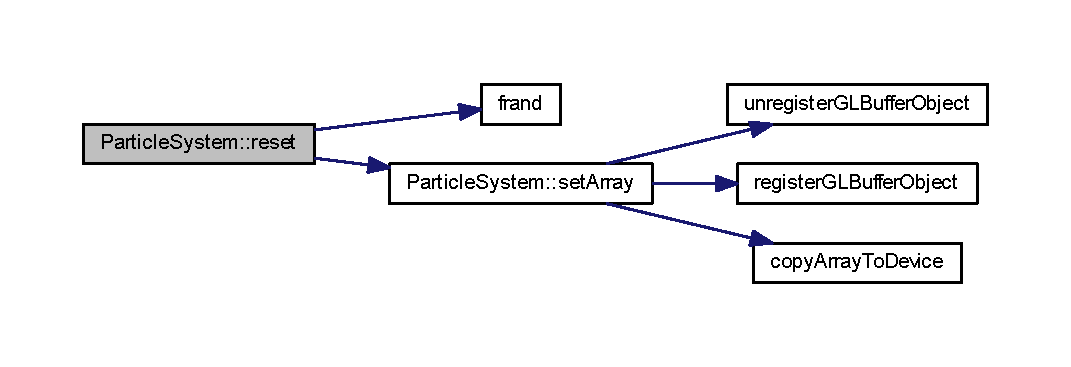
\includegraphics[width=350pt]{class_particle_system_a519070812dd9eb349f270c793c5f64b6_cgraph}
\end{center}
\end{figure}




Oto graf wywoływań tej funkcji\-:\nopagebreak
\begin{figure}[H]
\begin{center}
\leavevmode
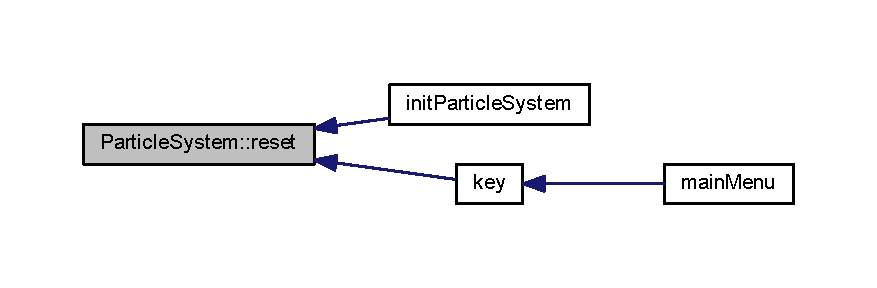
\includegraphics[width=350pt]{class_particle_system_a519070812dd9eb349f270c793c5f64b6_icgraph}
\end{center}
\end{figure}


\hypertarget{class_particle_system_aa792a66680e800832059854aab0d594d}{\index{Particle\-System@{Particle\-System}!set\-Array@{set\-Array}}
\index{set\-Array@{set\-Array}!ParticleSystem@{Particle\-System}}
\subsubsection[{set\-Array}]{\setlength{\rightskip}{0pt plus 5cm}void Particle\-System\-::set\-Array (
\begin{DoxyParamCaption}
\item[{{\bf Particle\-Array}}]{array, }
\item[{const float $\ast$}]{data, }
\item[{int}]{start, }
\item[{int}]{count}
\end{DoxyParamCaption}
)}}\label{class_particle_system_aa792a66680e800832059854aab0d594d}


Definicja w linii \hyperlink{particle_system_8cpp_source_l00374}{374} pliku \hyperlink{particle_system_8cpp_source}{particle\-System.\-cpp}.



Odwołuje się do \hyperlink{particle_system__cuda_8cu_source_l00077}{copy\-Array\-To\-Device()}, \hyperlink{particle_system_8h_source_l00152}{m\-\_\-b\-Initialized}, \hyperlink{particle_system_8h_source_l00152}{m\-\_\-b\-Use\-Open\-G\-L}, \hyperlink{particle_system_8h_source_l00184}{m\-\_\-cuda\-\_\-posvbo\-\_\-resource}, \hyperlink{particle_system_8h_source_l00165}{m\-\_\-d\-Vel}, \hyperlink{particle_system_8h_source_l00178}{m\-\_\-pos\-Vbo}, \hyperlink{particle_system_8h_source_l00038}{P\-O\-S\-I\-T\-I\-O\-N}, \hyperlink{particle_system__cuda_8cu_source_l00082}{register\-G\-L\-Buffer\-Object()}, \hyperlink{particle_system__cuda_8cu_source_l00088}{unregister\-G\-L\-Buffer\-Object()} i \hyperlink{particle_system_8h_source_l00039}{V\-E\-L\-O\-C\-I\-T\-Y}.



Odwołania w \hyperlink{particle_system_8cpp_source_l00485}{add\-Sphere()} i \hyperlink{particle_system_8cpp_source_l00436}{reset()}.


\begin{DoxyCode}
00375 \{
00376     assert(\hyperlink{class_particle_system_a21bbfba9d8701a70bc6fddbf4fc3f5bd}{m\_bInitialized});
00377 
00378     \textcolor{keywordflow}{switch} (array)
00379     \{
00380         \textcolor{keywordflow}{default}:
00381         \textcolor{keywordflow}{case} \hyperlink{class_particle_system_a332fbe57a36aaea5c18b4ea4fba6bbb3a9e9a2992d230a2674debf26e0e8e0299}{POSITION}:
00382             \{
00383                 \textcolor{keywordflow}{if} (\hyperlink{class_particle_system_a5d99413ffc0791e6aa9f02308caf7f1e}{m\_bUseOpenGL})
00384                 \{
00385                     \hyperlink{particle_system_8cuh_a9afef8c00ca779aae2d7484b45bce34c}{unregisterGLBufferObject}(
      \hyperlink{class_particle_system_a9c5de70c1705672e5722ad30dee1b14b}{m\_cuda\_posvbo\_resource});
00386                     glBindBuffer(GL\_ARRAY\_BUFFER, \hyperlink{class_particle_system_a31f9cccdf5dbae6f72867665bd8761e3}{m\_posVbo});
00387                     glBufferSubData(GL\_ARRAY\_BUFFER, start*4*\textcolor{keyword}{sizeof}(\textcolor{keywordtype}{float}), count*4*\textcolor{keyword}{sizeof}(\textcolor{keywordtype}{float}), data);
00388                     glBindBuffer(GL\_ARRAY\_BUFFER, 0);
00389                     \hyperlink{particle_system_8cuh_a4386a84282ceeaba09939817aa2a9c24}{registerGLBufferObject}(\hyperlink{class_particle_system_a31f9cccdf5dbae6f72867665bd8761e3}{m\_posVbo}, &
      \hyperlink{class_particle_system_a9c5de70c1705672e5722ad30dee1b14b}{m\_cuda\_posvbo\_resource});
00390                 \}
00391             \}
00392             \textcolor{keywordflow}{break};
00393 
00394         \textcolor{keywordflow}{case} \hyperlink{class_particle_system_a332fbe57a36aaea5c18b4ea4fba6bbb3a3702de73065f01b4f6ffa604b799e53d}{VELOCITY}:
00395             \hyperlink{particle_system_8cuh_ac4d4ecd921dbed6c2deef639ca295374}{copyArrayToDevice}(\hyperlink{class_particle_system_a5efd31a2fdba8d98b105f4e546964cb5}{m\_dVel}, data, start*4*\textcolor{keyword}{sizeof}(\textcolor{keywordtype}{float}), count*4*\textcolor{keyword}{sizeof}(\textcolor{keywordtype}{
      float}));
00396             \textcolor{keywordflow}{break};
00397     \}
00398 \}
\end{DoxyCode}


Oto graf wywołań dla tej funkcji\-:\nopagebreak
\begin{figure}[H]
\begin{center}
\leavevmode
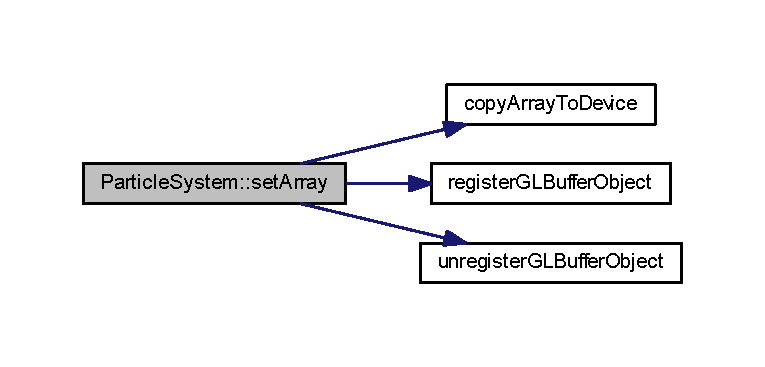
\includegraphics[width=350pt]{class_particle_system_aa792a66680e800832059854aab0d594d_cgraph}
\end{center}
\end{figure}




Oto graf wywoływań tej funkcji\-:\nopagebreak
\begin{figure}[H]
\begin{center}
\leavevmode
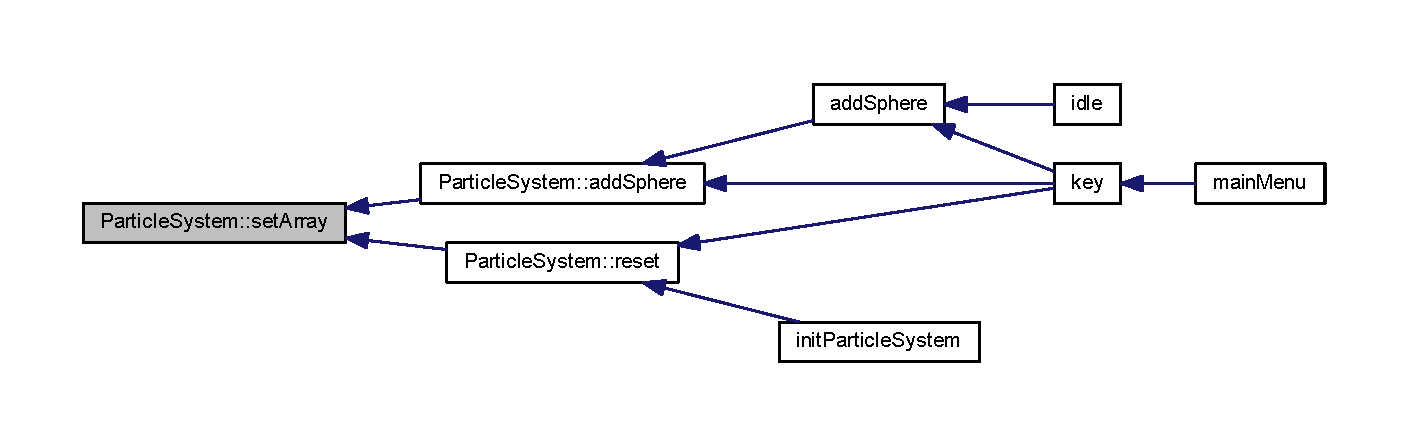
\includegraphics[width=350pt]{class_particle_system_aa792a66680e800832059854aab0d594d_icgraph}
\end{center}
\end{figure}


\hypertarget{class_particle_system_a97efe00aa29307ecae0165da33d4770a}{\index{Particle\-System@{Particle\-System}!set\-Big\-Radius@{set\-Big\-Radius}}
\index{set\-Big\-Radius@{set\-Big\-Radius}!ParticleSystem@{Particle\-System}}
\subsubsection[{set\-Big\-Radius}]{\setlength{\rightskip}{0pt plus 5cm}void Particle\-System\-::set\-Big\-Radius (
\begin{DoxyParamCaption}
\item[{float}]{x}
\end{DoxyParamCaption}
)\hspace{0.3cm}{\ttfamily [inline]}}}\label{class_particle_system_a97efe00aa29307ecae0165da33d4770a}


Definicja w linii \hyperlink{particle_system_8h_source_l00105}{105} pliku \hyperlink{particle_system_8h_source}{particle\-System.\-h}.



Odwołania w \hyperlink{particles_8cpp_source_l00248}{display()}.


\begin{DoxyCode}
00106                 \{
00107                         \hyperlink{class_particle_system_ab765472aed6a1b5f0d2f98a3a906c417}{m\_params}.\hyperlink{struct_sim_params_af41979948fdd8f76fe28ce2b43eb24cd}{bigradius}=x;
00108                 \}
\end{DoxyCode}


Oto graf wywoływań tej funkcji\-:\nopagebreak
\begin{figure}[H]
\begin{center}
\leavevmode
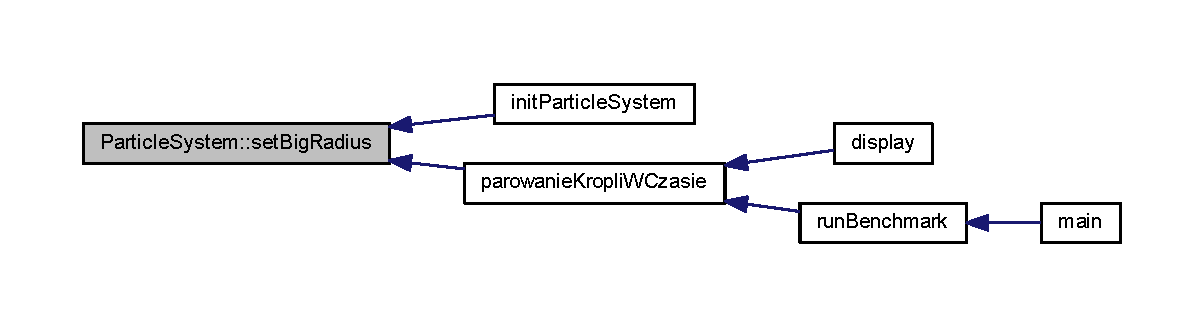
\includegraphics[width=310pt]{class_particle_system_a97efe00aa29307ecae0165da33d4770a_icgraph}
\end{center}
\end{figure}


\hypertarget{class_particle_system_aef02d293e3dc61c50fa6d085aa0b03de}{\index{Particle\-System@{Particle\-System}!set\-Collide\-Attraction@{set\-Collide\-Attraction}}
\index{set\-Collide\-Attraction@{set\-Collide\-Attraction}!ParticleSystem@{Particle\-System}}
\subsubsection[{set\-Collide\-Attraction}]{\setlength{\rightskip}{0pt plus 5cm}void Particle\-System\-::set\-Collide\-Attraction (
\begin{DoxyParamCaption}
\item[{float}]{x}
\end{DoxyParamCaption}
)\hspace{0.3cm}{\ttfamily [inline]}}}\label{class_particle_system_aef02d293e3dc61c50fa6d085aa0b03de}


Definicja w linii \hyperlink{particle_system_8h_source_l00100}{100} pliku \hyperlink{particle_system_8h_source}{particle\-System.\-h}.



Odwołania w \hyperlink{particles_8cpp_source_l00248}{display()}.


\begin{DoxyCode}
00101         \{
00102             \hyperlink{class_particle_system_ab765472aed6a1b5f0d2f98a3a906c417}{m\_params}.\hyperlink{struct_sim_params_acf7442ae8a49237861944271cb630d01}{attraction} = x;
00103         \}
\end{DoxyCode}


Oto graf wywoływań tej funkcji\-:\nopagebreak
\begin{figure}[H]
\begin{center}
\leavevmode
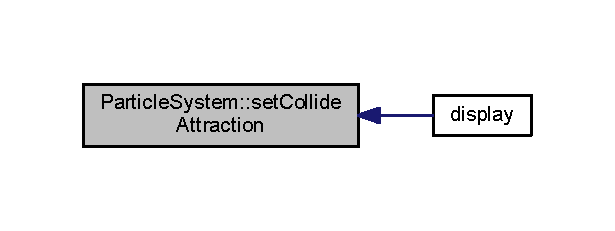
\includegraphics[width=295pt]{class_particle_system_aef02d293e3dc61c50fa6d085aa0b03de_icgraph}
\end{center}
\end{figure}


\hypertarget{class_particle_system_a8f8d21c7079c3a0e66558b9ec5bef597}{\index{Particle\-System@{Particle\-System}!set\-Collide\-Damping@{set\-Collide\-Damping}}
\index{set\-Collide\-Damping@{set\-Collide\-Damping}!ParticleSystem@{Particle\-System}}
\subsubsection[{set\-Collide\-Damping}]{\setlength{\rightskip}{0pt plus 5cm}void Particle\-System\-::set\-Collide\-Damping (
\begin{DoxyParamCaption}
\item[{float}]{x}
\end{DoxyParamCaption}
)\hspace{0.3cm}{\ttfamily [inline]}}}\label{class_particle_system_a8f8d21c7079c3a0e66558b9ec5bef597}


Definicja w linii \hyperlink{particle_system_8h_source_l00092}{92} pliku \hyperlink{particle_system_8h_source}{particle\-System.\-h}.



Odwołania w \hyperlink{particles_8cpp_source_l00248}{display()}.


\begin{DoxyCode}
00093         \{
00094             \hyperlink{class_particle_system_ab765472aed6a1b5f0d2f98a3a906c417}{m\_params}.\hyperlink{struct_sim_params_abf1644c671e60ebaf873d9167e755328}{damping} = x;
00095         \}
\end{DoxyCode}


Oto graf wywoływań tej funkcji\-:\nopagebreak
\begin{figure}[H]
\begin{center}
\leavevmode
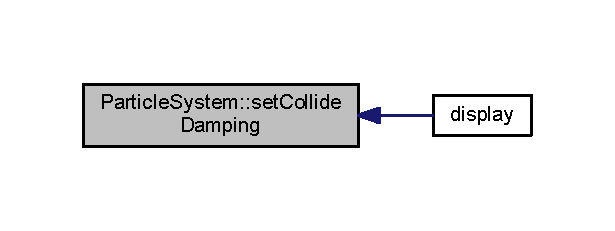
\includegraphics[width=295pt]{class_particle_system_a8f8d21c7079c3a0e66558b9ec5bef597_icgraph}
\end{center}
\end{figure}


\hypertarget{class_particle_system_a9c49794585cad649de400dc7375d7801}{\index{Particle\-System@{Particle\-System}!set\-Collider\-Pos@{set\-Collider\-Pos}}
\index{set\-Collider\-Pos@{set\-Collider\-Pos}!ParticleSystem@{Particle\-System}}
\subsubsection[{set\-Collider\-Pos}]{\setlength{\rightskip}{0pt plus 5cm}void Particle\-System\-::set\-Collider\-Pos (
\begin{DoxyParamCaption}
\item[{float3}]{x}
\end{DoxyParamCaption}
)\hspace{0.3cm}{\ttfamily [inline]}}}\label{class_particle_system_a9c49794585cad649de400dc7375d7801}


Definicja w linii \hyperlink{particle_system_8h_source_l00110}{110} pliku \hyperlink{particle_system_8h_source}{particle\-System.\-h}.


\begin{DoxyCode}
00111         \{
00112             \hyperlink{class_particle_system_ab765472aed6a1b5f0d2f98a3a906c417}{m\_params}.\hyperlink{struct_sim_params_aa27be265020f137f0a9cfbc3f1d2d9f8}{colliderPos} = x;
00113         \}
\end{DoxyCode}
\hypertarget{class_particle_system_aea667093542a1bdad65bdcb427e5625f}{\index{Particle\-System@{Particle\-System}!set\-Collide\-Shear@{set\-Collide\-Shear}}
\index{set\-Collide\-Shear@{set\-Collide\-Shear}!ParticleSystem@{Particle\-System}}
\subsubsection[{set\-Collide\-Shear}]{\setlength{\rightskip}{0pt plus 5cm}void Particle\-System\-::set\-Collide\-Shear (
\begin{DoxyParamCaption}
\item[{float}]{x}
\end{DoxyParamCaption}
)\hspace{0.3cm}{\ttfamily [inline]}}}\label{class_particle_system_aea667093542a1bdad65bdcb427e5625f}


Definicja w linii \hyperlink{particle_system_8h_source_l00096}{96} pliku \hyperlink{particle_system_8h_source}{particle\-System.\-h}.



Odwołania w \hyperlink{particles_8cpp_source_l00248}{display()}.


\begin{DoxyCode}
00097         \{
00098             \hyperlink{class_particle_system_ab765472aed6a1b5f0d2f98a3a906c417}{m\_params}.\hyperlink{struct_sim_params_ad48210724ada15a14a649b25ad61575b}{shear} = x;
00099         \}
\end{DoxyCode}


Oto graf wywoływań tej funkcji\-:\nopagebreak
\begin{figure}[H]
\begin{center}
\leavevmode
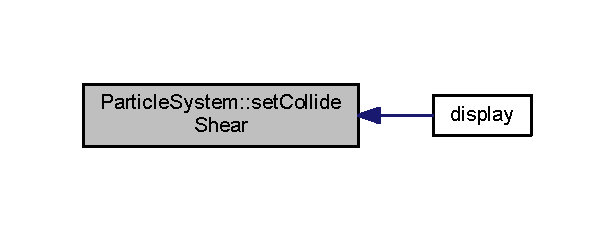
\includegraphics[width=295pt]{class_particle_system_aea667093542a1bdad65bdcb427e5625f_icgraph}
\end{center}
\end{figure}


\hypertarget{class_particle_system_a7ed53fca9ef126898d29314478ec8fd4}{\index{Particle\-System@{Particle\-System}!set\-Collide\-Spring@{set\-Collide\-Spring}}
\index{set\-Collide\-Spring@{set\-Collide\-Spring}!ParticleSystem@{Particle\-System}}
\subsubsection[{set\-Collide\-Spring}]{\setlength{\rightskip}{0pt plus 5cm}void Particle\-System\-::set\-Collide\-Spring (
\begin{DoxyParamCaption}
\item[{float}]{x}
\end{DoxyParamCaption}
)\hspace{0.3cm}{\ttfamily [inline]}}}\label{class_particle_system_a7ed53fca9ef126898d29314478ec8fd4}


Definicja w linii \hyperlink{particle_system_8h_source_l00088}{88} pliku \hyperlink{particle_system_8h_source}{particle\-System.\-h}.



Odwołania w \hyperlink{particles_8cpp_source_l00248}{display()}.


\begin{DoxyCode}
00089         \{
00090             \hyperlink{class_particle_system_ab765472aed6a1b5f0d2f98a3a906c417}{m\_params}.\hyperlink{struct_sim_params_a301314921adc7bce20d8955cf03cdf3f}{spring} = x;
00091         \}
\end{DoxyCode}


Oto graf wywoływań tej funkcji\-:\nopagebreak
\begin{figure}[H]
\begin{center}
\leavevmode
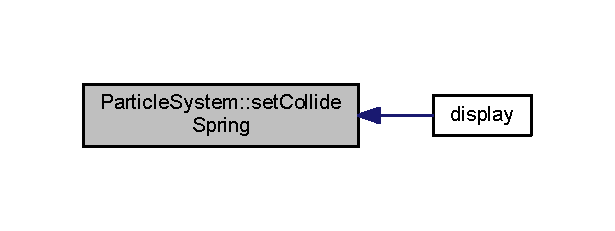
\includegraphics[width=295pt]{class_particle_system_a7ed53fca9ef126898d29314478ec8fd4_icgraph}
\end{center}
\end{figure}


\hypertarget{class_particle_system_aa26996b9ca13499b13f944f3aaeae10c}{\index{Particle\-System@{Particle\-System}!set\-Damping@{set\-Damping}}
\index{set\-Damping@{set\-Damping}!ParticleSystem@{Particle\-System}}
\subsubsection[{set\-Damping}]{\setlength{\rightskip}{0pt plus 5cm}void Particle\-System\-::set\-Damping (
\begin{DoxyParamCaption}
\item[{float}]{x}
\end{DoxyParamCaption}
)\hspace{0.3cm}{\ttfamily [inline]}}}\label{class_particle_system_aa26996b9ca13499b13f944f3aaeae10c}


Definicja w linii \hyperlink{particle_system_8h_source_l00079}{79} pliku \hyperlink{particle_system_8h_source}{particle\-System.\-h}.



Odwołania w \hyperlink{particles_8cpp_source_l00248}{display()}.


\begin{DoxyCode}
00080         \{
00081             \hyperlink{class_particle_system_ab765472aed6a1b5f0d2f98a3a906c417}{m\_params}.\hyperlink{struct_sim_params_a7058bad8c867d9d42d8c9d842638ebea}{globalDamping} = x;
00082         \}
\end{DoxyCode}


Oto graf wywoływań tej funkcji\-:\nopagebreak
\begin{figure}[H]
\begin{center}
\leavevmode
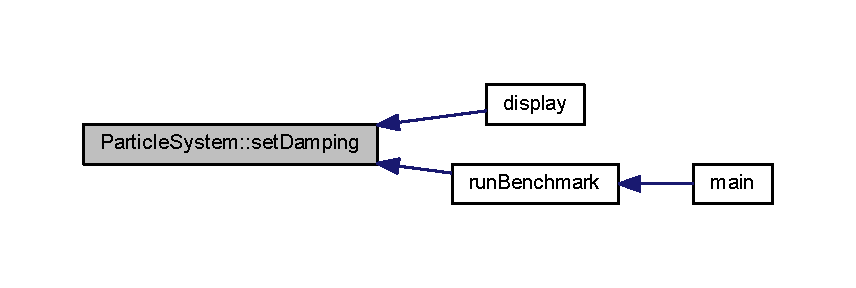
\includegraphics[width=304pt]{class_particle_system_aa26996b9ca13499b13f944f3aaeae10c_icgraph}
\end{center}
\end{figure}


\hypertarget{class_particle_system_a755f64f917389ef41df81b663d1f5bd2}{\index{Particle\-System@{Particle\-System}!set\-Gravity@{set\-Gravity}}
\index{set\-Gravity@{set\-Gravity}!ParticleSystem@{Particle\-System}}
\subsubsection[{set\-Gravity}]{\setlength{\rightskip}{0pt plus 5cm}void Particle\-System\-::set\-Gravity (
\begin{DoxyParamCaption}
\item[{float}]{x}
\end{DoxyParamCaption}
)\hspace{0.3cm}{\ttfamily [inline]}}}\label{class_particle_system_a755f64f917389ef41df81b663d1f5bd2}


Definicja w linii \hyperlink{particle_system_8h_source_l00083}{83} pliku \hyperlink{particle_system_8h_source}{particle\-System.\-h}.



Odwołania w \hyperlink{particles_8cpp_source_l00248}{display()}.


\begin{DoxyCode}
00084         \{
00085             \hyperlink{class_particle_system_ab765472aed6a1b5f0d2f98a3a906c417}{m\_params}.\hyperlink{struct_sim_params_ae7508eba5dd90859215b59d19e001bb9}{gravity} = make\_float3(0.0f, x, 0.0f);
00086         \}
\end{DoxyCode}


Oto graf wywoływań tej funkcji\-:\nopagebreak
\begin{figure}[H]
\begin{center}
\leavevmode
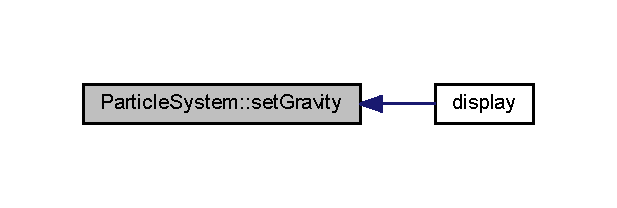
\includegraphics[width=296pt]{class_particle_system_a755f64f917389ef41df81b663d1f5bd2_icgraph}
\end{center}
\end{figure}


\hypertarget{class_particle_system_a11f55976f6ef34dceea208fbe06694cd}{\index{Particle\-System@{Particle\-System}!set\-Iterations@{set\-Iterations}}
\index{set\-Iterations@{set\-Iterations}!ParticleSystem@{Particle\-System}}
\subsubsection[{set\-Iterations}]{\setlength{\rightskip}{0pt plus 5cm}void Particle\-System\-::set\-Iterations (
\begin{DoxyParamCaption}
\item[{int}]{i}
\end{DoxyParamCaption}
)\hspace{0.3cm}{\ttfamily [inline]}}}\label{class_particle_system_a11f55976f6ef34dceea208fbe06694cd}


Definicja w linii \hyperlink{particle_system_8h_source_l00074}{74} pliku \hyperlink{particle_system_8h_source}{particle\-System.\-h}.



Odwołuje się do \hyperlink{particle_system_8h_source_l00194}{m\-\_\-solver\-Iterations}.



Odwołania w \hyperlink{particles_8cpp_source_l00248}{display()}.


\begin{DoxyCode}
00075         \{
00076             \hyperlink{class_particle_system_a7b4b053433c052518b8ecce1b02000f5}{m\_solverIterations} = i;
00077         \}
\end{DoxyCode}


Oto graf wywoływań tej funkcji\-:\nopagebreak
\begin{figure}[H]
\begin{center}
\leavevmode
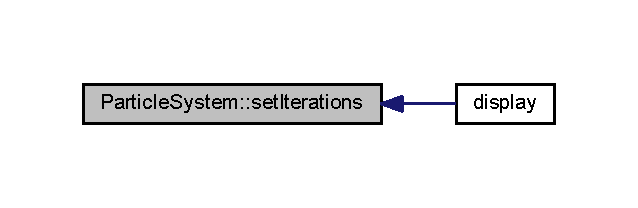
\includegraphics[width=306pt]{class_particle_system_a11f55976f6ef34dceea208fbe06694cd_icgraph}
\end{center}
\end{figure}


\hypertarget{class_particle_system_a166fd86f020b6024d7d42723762d7cb2}{\index{Particle\-System@{Particle\-System}!update@{update}}
\index{update@{update}!ParticleSystem@{Particle\-System}}
\subsubsection[{update}]{\setlength{\rightskip}{0pt plus 5cm}void Particle\-System\-::update (
\begin{DoxyParamCaption}
\item[{float}]{delta\-Time}
\end{DoxyParamCaption}
)}}\label{class_particle_system_a166fd86f020b6024d7d42723762d7cb2}


Definicja w linii \hyperlink{particle_system_8cpp_source_l00238}{238} pliku \hyperlink{particle_system_8cpp_source}{particle\-System.\-cpp}.



Odwołuje się do \hyperlink{particle_system__cuda_8cu_source_l00157}{calc\-Hash()}, \hyperlink{particle_system__cuda_8cu_source_l00219}{collide()}, \hyperlink{particle_system__cuda_8cu_source_l00143}{integrate\-System()}, \hyperlink{particle_system_8h_source_l00152}{m\-\_\-b\-Initialized}, \hyperlink{particle_system_8h_source_l00152}{m\-\_\-b\-Use\-Open\-G\-L}, \hyperlink{particle_system_8h_source_l00184}{m\-\_\-cuda\-\_\-posvbo\-\_\-resource}, \hyperlink{particle_system_8h_source_l00181}{m\-\_\-cuda\-Pos\-V\-B\-O}, \hyperlink{particle_system_8h_source_l00174}{m\-\_\-d\-Cell\-End}, \hyperlink{particle_system_8h_source_l00173}{m\-\_\-d\-Cell\-Start}, \hyperlink{particle_system_8h_source_l00171}{m\-\_\-d\-Grid\-Particle\-Hash}, \hyperlink{particle_system_8h_source_l00172}{m\-\_\-d\-Grid\-Particle\-Index}, \hyperlink{particle_system_8h_source_l00167}{m\-\_\-d\-Sorted\-Pos}, \hyperlink{particle_system_8h_source_l00168}{m\-\_\-d\-Sorted\-Vel}, \hyperlink{particle_system_8h_source_l00165}{m\-\_\-d\-Vel}, \hyperlink{particle_system_8h_source_l00190}{m\-\_\-num\-Grid\-Cells}, \hyperlink{particle_system_8h_source_l00153}{m\-\_\-num\-Particles}, \hyperlink{particle_system__cuda_8cu_source_l00093}{map\-G\-L\-Buffer\-Object()}, \hyperlink{particle_system__cuda_8cu_source_l00178}{reorder\-Data\-And\-Find\-Cell\-Start()}, \hyperlink{particle_system__cuda_8cu_source_l00263}{sort\-Particles()} i \hyperlink{particle_system__cuda_8cu_source_l00103}{unmap\-G\-L\-Buffer\-Object()}.



Odwołania w \hyperlink{particles_8cpp_source_l00248}{display()}, \hyperlink{particles_8cpp_source_l00520}{key()} i \hyperlink{particles_8cpp_source_l00194}{run\-Benchmark()}.


\begin{DoxyCode}
00239 \{
00240     assert(\hyperlink{class_particle_system_a21bbfba9d8701a70bc6fddbf4fc3f5bd}{m\_bInitialized});
00241 
00242     \textcolor{keywordtype}{float} *dPos;
00243 
00244     \textcolor{keywordflow}{if} (\hyperlink{class_particle_system_a5d99413ffc0791e6aa9f02308caf7f1e}{m\_bUseOpenGL})
00245     \{
00246         dPos = (\textcolor{keywordtype}{float} *) \hyperlink{particle_system_8cuh_aa491077afd740a269815eb9ce81c8642}{mapGLBufferObject}(&
      \hyperlink{class_particle_system_a9c5de70c1705672e5722ad30dee1b14b}{m\_cuda\_posvbo\_resource});
00247     \}
00248     \textcolor{keywordflow}{else}
00249     \{
00250         dPos = (\textcolor{keywordtype}{float} *) \hyperlink{class_particle_system_aba18245745f621d90186862f1a559d9e}{m\_cudaPosVBO};
00251     \}
00252 
00253     \textcolor{comment}{// update constants}
00254     \hyperlink{particle_system_8cuh_a342176dbaba2668312c45e1a1423fc4e}{setParameters}(&\hyperlink{class_particle_system_ab765472aed6a1b5f0d2f98a3a906c417}{m\_params});
00255 
00256     \textcolor{comment}{// integrate}
00257     \hyperlink{particle_system_8cuh_a34e9db8b801cd537e5ae5a4a886e020c}{integrateSystem}(
00258         dPos,
00259         \hyperlink{class_particle_system_a5efd31a2fdba8d98b105f4e546964cb5}{m\_dVel},
00260         deltaTime,
00261         \hyperlink{class_particle_system_a23d238efa80a647d4b6cde034f486a91}{m\_numParticles});
00262 
00263     \textcolor{comment}{// calculate grid hash}
00264     \hyperlink{particle_system_8cuh_ae0a4037d25e768622443077546399cf2}{calcHash}(
00265         \hyperlink{class_particle_system_ab44080655971a5501eaee6ad7355a139}{m\_dGridParticleHash},
00266         \hyperlink{class_particle_system_a1a67fc1e3ffd4e64f55a2a315c49c74c}{m\_dGridParticleIndex},
00267         dPos,
00268         \hyperlink{class_particle_system_a23d238efa80a647d4b6cde034f486a91}{m\_numParticles});
00269 
00270     \textcolor{comment}{// sort particles based on hash}
00271     \hyperlink{particle_system_8cuh_ac71da7e4672a2732a098ba933a799257}{sortParticles}(\hyperlink{class_particle_system_ab44080655971a5501eaee6ad7355a139}{m\_dGridParticleHash}, 
      \hyperlink{class_particle_system_a1a67fc1e3ffd4e64f55a2a315c49c74c}{m\_dGridParticleIndex}, \hyperlink{class_particle_system_a23d238efa80a647d4b6cde034f486a91}{m\_numParticles});
00272 
00273     \textcolor{comment}{// reorder particle arrays into sorted order and}
00274     \textcolor{comment}{// find start and end of each cell}
00275     \hyperlink{particle_system_8cuh_ac72ccd068434c46c2f901c751d53be1d}{reorderDataAndFindCellStart}(
00276         \hyperlink{class_particle_system_a137909a8b34f7a42e50cd0fcc86bb784}{m\_dCellStart},
00277         \hyperlink{class_particle_system_a3a0b9c760c2bfcf811d54b8194ebea01}{m\_dCellEnd},
00278         \hyperlink{class_particle_system_ab60e8b5a312b2f400b10dfba5153fc3c}{m\_dSortedPos},
00279         \hyperlink{class_particle_system_a69122523117954fb5defb8b38e0f46f3}{m\_dSortedVel},
00280         \hyperlink{class_particle_system_ab44080655971a5501eaee6ad7355a139}{m\_dGridParticleHash},
00281         \hyperlink{class_particle_system_a1a67fc1e3ffd4e64f55a2a315c49c74c}{m\_dGridParticleIndex},
00282         dPos,
00283         \hyperlink{class_particle_system_a5efd31a2fdba8d98b105f4e546964cb5}{m\_dVel},
00284         \hyperlink{class_particle_system_a23d238efa80a647d4b6cde034f486a91}{m\_numParticles},
00285         \hyperlink{class_particle_system_aa1ef17d723af5d7a4685e8fd57e9ca89}{m\_numGridCells});
00286 
00287     \textcolor{comment}{// process collisions}
00288     \hyperlink{particle_system_8cuh_a917d67e2ed45ea11da51ac5d7004ddfd}{collide}(
00289         \hyperlink{class_particle_system_a5efd31a2fdba8d98b105f4e546964cb5}{m\_dVel},
00290         \hyperlink{class_particle_system_ab60e8b5a312b2f400b10dfba5153fc3c}{m\_dSortedPos},
00291         \hyperlink{class_particle_system_a69122523117954fb5defb8b38e0f46f3}{m\_dSortedVel},
00292         \hyperlink{class_particle_system_a1a67fc1e3ffd4e64f55a2a315c49c74c}{m\_dGridParticleIndex},
00293         \hyperlink{class_particle_system_a137909a8b34f7a42e50cd0fcc86bb784}{m\_dCellStart},
00294         \hyperlink{class_particle_system_a3a0b9c760c2bfcf811d54b8194ebea01}{m\_dCellEnd},
00295         \hyperlink{class_particle_system_a23d238efa80a647d4b6cde034f486a91}{m\_numParticles},
00296         \hyperlink{class_particle_system_aa1ef17d723af5d7a4685e8fd57e9ca89}{m\_numGridCells});
00297 
00298     \textcolor{comment}{// note: do unmap at end here to avoid unnecessary graphics/CUDA context switch}
00299     \textcolor{keywordflow}{if} (\hyperlink{class_particle_system_a5d99413ffc0791e6aa9f02308caf7f1e}{m\_bUseOpenGL})
00300     \{
00301         \hyperlink{particle_system_8cuh_a98c3325419b7528d34a51ca7972d7095}{unmapGLBufferObject}(\hyperlink{class_particle_system_a9c5de70c1705672e5722ad30dee1b14b}{m\_cuda\_posvbo\_resource});
00302     \}
00303 \}
\end{DoxyCode}


Oto graf wywołań dla tej funkcji\-:\nopagebreak
\begin{figure}[H]
\begin{center}
\leavevmode
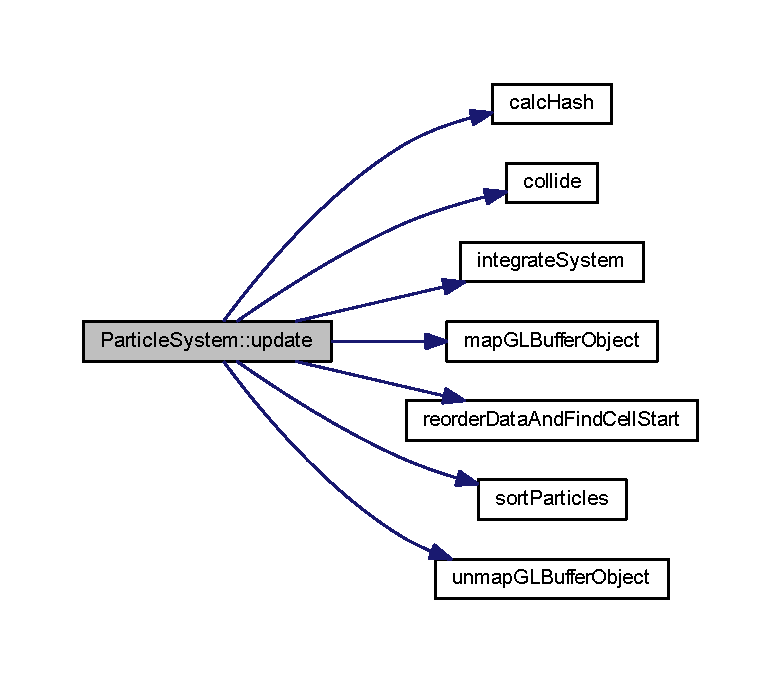
\includegraphics[width=350pt]{class_particle_system_a166fd86f020b6024d7d42723762d7cb2_cgraph}
\end{center}
\end{figure}




Oto graf wywoływań tej funkcji\-:\nopagebreak
\begin{figure}[H]
\begin{center}
\leavevmode
\includegraphics[width=350pt]{class_particle_system_a166fd86f020b6024d7d42723762d7cb2_icgraph}
\end{center}
\end{figure}




\subsection{Dokumentacja atrybutów składowych}
\hypertarget{class_particle_system_a21bbfba9d8701a70bc6fddbf4fc3f5bd}{\index{Particle\-System@{Particle\-System}!m\-\_\-b\-Initialized@{m\-\_\-b\-Initialized}}
\index{m\-\_\-b\-Initialized@{m\-\_\-b\-Initialized}!ParticleSystem@{Particle\-System}}
\subsubsection[{m\-\_\-b\-Initialized}]{\setlength{\rightskip}{0pt plus 5cm}bool Particle\-System\-::m\-\_\-b\-Initialized\hspace{0.3cm}{\ttfamily [protected]}}}\label{class_particle_system_a21bbfba9d8701a70bc6fddbf4fc3f5bd}


Definicja w linii \hyperlink{particle_system_8h_source_l00152}{152} pliku \hyperlink{particle_system_8h_source}{particle\-System.\-h}.



Odwołania w \hyperlink{particle_system_8cpp_source_l00205}{\-\_\-finalize()}, \hyperlink{particle_system_8cpp_source_l00123}{\-\_\-initialize()}, \hyperlink{particle_system_8cpp_source_l00346}{get\-Array()}, \hyperlink{particle_system_8cpp_source_l00033}{Particle\-System()}, \hyperlink{particle_system_8cpp_source_l00374}{set\-Array()} i \hyperlink{particle_system_8cpp_source_l00238}{update()}.

\hypertarget{class_particle_system_a5d99413ffc0791e6aa9f02308caf7f1e}{\index{Particle\-System@{Particle\-System}!m\-\_\-b\-Use\-Open\-G\-L@{m\-\_\-b\-Use\-Open\-G\-L}}
\index{m\-\_\-b\-Use\-Open\-G\-L@{m\-\_\-b\-Use\-Open\-G\-L}!ParticleSystem@{Particle\-System}}
\subsubsection[{m\-\_\-b\-Use\-Open\-G\-L}]{\setlength{\rightskip}{0pt plus 5cm}bool Particle\-System\-::m\-\_\-b\-Use\-Open\-G\-L\hspace{0.3cm}{\ttfamily [protected]}}}\label{class_particle_system_a5d99413ffc0791e6aa9f02308caf7f1e}


Definicja w linii \hyperlink{particle_system_8h_source_l00152}{152} pliku \hyperlink{particle_system_8h_source}{particle\-System.\-h}.



Odwołania w \hyperlink{particle_system_8cpp_source_l00205}{\-\_\-finalize()}, \hyperlink{particle_system_8cpp_source_l00123}{\-\_\-initialize()}, \hyperlink{particle_system_8cpp_source_l00033}{Particle\-System()}, \hyperlink{particle_system_8cpp_source_l00374}{set\-Array()} i \hyperlink{particle_system_8cpp_source_l00238}{update()}.

\hypertarget{class_particle_system_a96b05c719006c9e3eaed759f54a49c7f}{\index{Particle\-System@{Particle\-System}!m\-\_\-color\-V\-B\-O@{m\-\_\-color\-V\-B\-O}}
\index{m\-\_\-color\-V\-B\-O@{m\-\_\-color\-V\-B\-O}!ParticleSystem@{Particle\-System}}
\subsubsection[{m\-\_\-color\-V\-B\-O}]{\setlength{\rightskip}{0pt plus 5cm}{\bf uint} Particle\-System\-::m\-\_\-color\-V\-B\-O\hspace{0.3cm}{\ttfamily [protected]}}}\label{class_particle_system_a96b05c719006c9e3eaed759f54a49c7f}


Definicja w linii \hyperlink{particle_system_8h_source_l00179}{179} pliku \hyperlink{particle_system_8h_source}{particle\-System.\-h}.



Odwołania w \hyperlink{particle_system_8cpp_source_l00123}{\-\_\-initialize()} i \hyperlink{particle_system_8h_source_l00057}{get\-Color\-Buffer()}.

\hypertarget{class_particle_system_a140043869727535abc08609b835b98fc}{\index{Particle\-System@{Particle\-System}!m\-\_\-cuda\-\_\-colorvbo\-\_\-resource@{m\-\_\-cuda\-\_\-colorvbo\-\_\-resource}}
\index{m\-\_\-cuda\-\_\-colorvbo\-\_\-resource@{m\-\_\-cuda\-\_\-colorvbo\-\_\-resource}!ParticleSystem@{Particle\-System}}
\subsubsection[{m\-\_\-cuda\-\_\-colorvbo\-\_\-resource}]{\setlength{\rightskip}{0pt plus 5cm}struct cuda\-Graphics\-Resource$\ast$ Particle\-System\-::m\-\_\-cuda\-\_\-colorvbo\-\_\-resource\hspace{0.3cm}{\ttfamily [protected]}}}\label{class_particle_system_a140043869727535abc08609b835b98fc}


Definicja w linii \hyperlink{particle_system_8h_source_l00185}{185} pliku \hyperlink{particle_system_8h_source}{particle\-System.\-h}.



Odwołania w \hyperlink{particle_system_8cpp_source_l00123}{\-\_\-initialize()}.

\hypertarget{class_particle_system_a9c5de70c1705672e5722ad30dee1b14b}{\index{Particle\-System@{Particle\-System}!m\-\_\-cuda\-\_\-posvbo\-\_\-resource@{m\-\_\-cuda\-\_\-posvbo\-\_\-resource}}
\index{m\-\_\-cuda\-\_\-posvbo\-\_\-resource@{m\-\_\-cuda\-\_\-posvbo\-\_\-resource}!ParticleSystem@{Particle\-System}}
\subsubsection[{m\-\_\-cuda\-\_\-posvbo\-\_\-resource}]{\setlength{\rightskip}{0pt plus 5cm}struct cuda\-Graphics\-Resource$\ast$ Particle\-System\-::m\-\_\-cuda\-\_\-posvbo\-\_\-resource\hspace{0.3cm}{\ttfamily [protected]}}}\label{class_particle_system_a9c5de70c1705672e5722ad30dee1b14b}


Definicja w linii \hyperlink{particle_system_8h_source_l00184}{184} pliku \hyperlink{particle_system_8h_source}{particle\-System.\-h}.



Odwołania w \hyperlink{particle_system_8cpp_source_l00205}{\-\_\-finalize()}, \hyperlink{particle_system_8cpp_source_l00123}{\-\_\-initialize()}, \hyperlink{particle_system_8cpp_source_l00331}{dump\-Particles()}, \hyperlink{particle_system_8cpp_source_l00346}{get\-Array()}, \hyperlink{particle_system_8cpp_source_l00374}{set\-Array()} i \hyperlink{particle_system_8cpp_source_l00238}{update()}.

\hypertarget{class_particle_system_a39d210b57da5f7f4a2c23f4fc0b43ea1}{\index{Particle\-System@{Particle\-System}!m\-\_\-cuda\-Color\-V\-B\-O@{m\-\_\-cuda\-Color\-V\-B\-O}}
\index{m\-\_\-cuda\-Color\-V\-B\-O@{m\-\_\-cuda\-Color\-V\-B\-O}!ParticleSystem@{Particle\-System}}
\subsubsection[{m\-\_\-cuda\-Color\-V\-B\-O}]{\setlength{\rightskip}{0pt plus 5cm}float$\ast$ Particle\-System\-::m\-\_\-cuda\-Color\-V\-B\-O\hspace{0.3cm}{\ttfamily [protected]}}}\label{class_particle_system_a39d210b57da5f7f4a2c23f4fc0b43ea1}


Definicja w linii \hyperlink{particle_system_8h_source_l00182}{182} pliku \hyperlink{particle_system_8h_source}{particle\-System.\-h}.



Odwołania w \hyperlink{particle_system_8h_source_l00066}{get\-Cuda\-Color\-V\-B\-O()}.

\hypertarget{class_particle_system_aba18245745f621d90186862f1a559d9e}{\index{Particle\-System@{Particle\-System}!m\-\_\-cuda\-Pos\-V\-B\-O@{m\-\_\-cuda\-Pos\-V\-B\-O}}
\index{m\-\_\-cuda\-Pos\-V\-B\-O@{m\-\_\-cuda\-Pos\-V\-B\-O}!ParticleSystem@{Particle\-System}}
\subsubsection[{m\-\_\-cuda\-Pos\-V\-B\-O}]{\setlength{\rightskip}{0pt plus 5cm}float$\ast$ Particle\-System\-::m\-\_\-cuda\-Pos\-V\-B\-O\hspace{0.3cm}{\ttfamily [protected]}}}\label{class_particle_system_aba18245745f621d90186862f1a559d9e}


Definicja w linii \hyperlink{particle_system_8h_source_l00181}{181} pliku \hyperlink{particle_system_8h_source}{particle\-System.\-h}.



Odwołania w \hyperlink{particle_system_8h_source_l00062}{get\-Cuda\-Pos\-V\-B\-O()} i \hyperlink{particle_system_8cpp_source_l00238}{update()}.

\hypertarget{class_particle_system_a3a0b9c760c2bfcf811d54b8194ebea01}{\index{Particle\-System@{Particle\-System}!m\-\_\-d\-Cell\-End@{m\-\_\-d\-Cell\-End}}
\index{m\-\_\-d\-Cell\-End@{m\-\_\-d\-Cell\-End}!ParticleSystem@{Particle\-System}}
\subsubsection[{m\-\_\-d\-Cell\-End}]{\setlength{\rightskip}{0pt plus 5cm}{\bf uint}$\ast$ Particle\-System\-::m\-\_\-d\-Cell\-End\hspace{0.3cm}{\ttfamily [protected]}}}\label{class_particle_system_a3a0b9c760c2bfcf811d54b8194ebea01}


Definicja w linii \hyperlink{particle_system_8h_source_l00174}{174} pliku \hyperlink{particle_system_8h_source}{particle\-System.\-h}.



Odwołania w \hyperlink{particle_system_8cpp_source_l00205}{\-\_\-finalize()}, \hyperlink{particle_system_8cpp_source_l00123}{\-\_\-initialize()}, \hyperlink{particle_system_8cpp_source_l00306}{dump\-Grid()} i \hyperlink{particle_system_8cpp_source_l00238}{update()}.

\hypertarget{class_particle_system_a137909a8b34f7a42e50cd0fcc86bb784}{\index{Particle\-System@{Particle\-System}!m\-\_\-d\-Cell\-Start@{m\-\_\-d\-Cell\-Start}}
\index{m\-\_\-d\-Cell\-Start@{m\-\_\-d\-Cell\-Start}!ParticleSystem@{Particle\-System}}
\subsubsection[{m\-\_\-d\-Cell\-Start}]{\setlength{\rightskip}{0pt plus 5cm}{\bf uint}$\ast$ Particle\-System\-::m\-\_\-d\-Cell\-Start\hspace{0.3cm}{\ttfamily [protected]}}}\label{class_particle_system_a137909a8b34f7a42e50cd0fcc86bb784}


Definicja w linii \hyperlink{particle_system_8h_source_l00173}{173} pliku \hyperlink{particle_system_8h_source}{particle\-System.\-h}.



Odwołania w \hyperlink{particle_system_8cpp_source_l00205}{\-\_\-finalize()}, \hyperlink{particle_system_8cpp_source_l00123}{\-\_\-initialize()}, \hyperlink{particle_system_8cpp_source_l00306}{dump\-Grid()} i \hyperlink{particle_system_8cpp_source_l00238}{update()}.

\hypertarget{class_particle_system_ab44080655971a5501eaee6ad7355a139}{\index{Particle\-System@{Particle\-System}!m\-\_\-d\-Grid\-Particle\-Hash@{m\-\_\-d\-Grid\-Particle\-Hash}}
\index{m\-\_\-d\-Grid\-Particle\-Hash@{m\-\_\-d\-Grid\-Particle\-Hash}!ParticleSystem@{Particle\-System}}
\subsubsection[{m\-\_\-d\-Grid\-Particle\-Hash}]{\setlength{\rightskip}{0pt plus 5cm}{\bf uint}$\ast$ Particle\-System\-::m\-\_\-d\-Grid\-Particle\-Hash\hspace{0.3cm}{\ttfamily [protected]}}}\label{class_particle_system_ab44080655971a5501eaee6ad7355a139}


Definicja w linii \hyperlink{particle_system_8h_source_l00171}{171} pliku \hyperlink{particle_system_8h_source}{particle\-System.\-h}.



Odwołania w \hyperlink{particle_system_8cpp_source_l00205}{\-\_\-finalize()}, \hyperlink{particle_system_8cpp_source_l00123}{\-\_\-initialize()} i \hyperlink{particle_system_8cpp_source_l00238}{update()}.

\hypertarget{class_particle_system_a1a67fc1e3ffd4e64f55a2a315c49c74c}{\index{Particle\-System@{Particle\-System}!m\-\_\-d\-Grid\-Particle\-Index@{m\-\_\-d\-Grid\-Particle\-Index}}
\index{m\-\_\-d\-Grid\-Particle\-Index@{m\-\_\-d\-Grid\-Particle\-Index}!ParticleSystem@{Particle\-System}}
\subsubsection[{m\-\_\-d\-Grid\-Particle\-Index}]{\setlength{\rightskip}{0pt plus 5cm}{\bf uint}$\ast$ Particle\-System\-::m\-\_\-d\-Grid\-Particle\-Index\hspace{0.3cm}{\ttfamily [protected]}}}\label{class_particle_system_a1a67fc1e3ffd4e64f55a2a315c49c74c}


Definicja w linii \hyperlink{particle_system_8h_source_l00172}{172} pliku \hyperlink{particle_system_8h_source}{particle\-System.\-h}.



Odwołania w \hyperlink{particle_system_8cpp_source_l00205}{\-\_\-finalize()}, \hyperlink{particle_system_8cpp_source_l00123}{\-\_\-initialize()} i \hyperlink{particle_system_8cpp_source_l00238}{update()}.

\hypertarget{class_particle_system_afff6217d2726217dff77c81ef3c23bfa}{\index{Particle\-System@{Particle\-System}!m\-\_\-d\-Pos@{m\-\_\-d\-Pos}}
\index{m\-\_\-d\-Pos@{m\-\_\-d\-Pos}!ParticleSystem@{Particle\-System}}
\subsubsection[{m\-\_\-d\-Pos}]{\setlength{\rightskip}{0pt plus 5cm}float$\ast$ Particle\-System\-::m\-\_\-d\-Pos\hspace{0.3cm}{\ttfamily [protected]}}}\label{class_particle_system_afff6217d2726217dff77c81ef3c23bfa}


Definicja w linii \hyperlink{particle_system_8h_source_l00164}{164} pliku \hyperlink{particle_system_8h_source}{particle\-System.\-h}.



Odwołania w \hyperlink{particle_system_8cpp_source_l00346}{get\-Array()} i \hyperlink{particle_system_8cpp_source_l00033}{Particle\-System()}.

\hypertarget{class_particle_system_ab60e8b5a312b2f400b10dfba5153fc3c}{\index{Particle\-System@{Particle\-System}!m\-\_\-d\-Sorted\-Pos@{m\-\_\-d\-Sorted\-Pos}}
\index{m\-\_\-d\-Sorted\-Pos@{m\-\_\-d\-Sorted\-Pos}!ParticleSystem@{Particle\-System}}
\subsubsection[{m\-\_\-d\-Sorted\-Pos}]{\setlength{\rightskip}{0pt plus 5cm}float$\ast$ Particle\-System\-::m\-\_\-d\-Sorted\-Pos\hspace{0.3cm}{\ttfamily [protected]}}}\label{class_particle_system_ab60e8b5a312b2f400b10dfba5153fc3c}


Definicja w linii \hyperlink{particle_system_8h_source_l00167}{167} pliku \hyperlink{particle_system_8h_source}{particle\-System.\-h}.



Odwołania w \hyperlink{particle_system_8cpp_source_l00205}{\-\_\-finalize()}, \hyperlink{particle_system_8cpp_source_l00123}{\-\_\-initialize()} i \hyperlink{particle_system_8cpp_source_l00238}{update()}.

\hypertarget{class_particle_system_a69122523117954fb5defb8b38e0f46f3}{\index{Particle\-System@{Particle\-System}!m\-\_\-d\-Sorted\-Vel@{m\-\_\-d\-Sorted\-Vel}}
\index{m\-\_\-d\-Sorted\-Vel@{m\-\_\-d\-Sorted\-Vel}!ParticleSystem@{Particle\-System}}
\subsubsection[{m\-\_\-d\-Sorted\-Vel}]{\setlength{\rightskip}{0pt plus 5cm}float$\ast$ Particle\-System\-::m\-\_\-d\-Sorted\-Vel\hspace{0.3cm}{\ttfamily [protected]}}}\label{class_particle_system_a69122523117954fb5defb8b38e0f46f3}


Definicja w linii \hyperlink{particle_system_8h_source_l00168}{168} pliku \hyperlink{particle_system_8h_source}{particle\-System.\-h}.



Odwołania w \hyperlink{particle_system_8cpp_source_l00205}{\-\_\-finalize()}, \hyperlink{particle_system_8cpp_source_l00123}{\-\_\-initialize()} i \hyperlink{particle_system_8cpp_source_l00238}{update()}.

\hypertarget{class_particle_system_a5efd31a2fdba8d98b105f4e546964cb5}{\index{Particle\-System@{Particle\-System}!m\-\_\-d\-Vel@{m\-\_\-d\-Vel}}
\index{m\-\_\-d\-Vel@{m\-\_\-d\-Vel}!ParticleSystem@{Particle\-System}}
\subsubsection[{m\-\_\-d\-Vel}]{\setlength{\rightskip}{0pt plus 5cm}float$\ast$ Particle\-System\-::m\-\_\-d\-Vel\hspace{0.3cm}{\ttfamily [protected]}}}\label{class_particle_system_a5efd31a2fdba8d98b105f4e546964cb5}


Definicja w linii \hyperlink{particle_system_8h_source_l00165}{165} pliku \hyperlink{particle_system_8h_source}{particle\-System.\-h}.



Odwołania w \hyperlink{particle_system_8cpp_source_l00205}{\-\_\-finalize()}, \hyperlink{particle_system_8cpp_source_l00123}{\-\_\-initialize()}, \hyperlink{particle_system_8cpp_source_l00331}{dump\-Particles()}, \hyperlink{particle_system_8cpp_source_l00346}{get\-Array()}, \hyperlink{particle_system_8cpp_source_l00033}{Particle\-System()}, \hyperlink{particle_system_8cpp_source_l00374}{set\-Array()} i \hyperlink{particle_system_8cpp_source_l00238}{update()}.

\hypertarget{class_particle_system_ad555b31501a258d776e8c72c96178aa0}{\index{Particle\-System@{Particle\-System}!m\-\_\-grid\-Size@{m\-\_\-grid\-Size}}
\index{m\-\_\-grid\-Size@{m\-\_\-grid\-Size}!ParticleSystem@{Particle\-System}}
\subsubsection[{m\-\_\-grid\-Size}]{\setlength{\rightskip}{0pt plus 5cm}uint3 Particle\-System\-::m\-\_\-grid\-Size\hspace{0.3cm}{\ttfamily [protected]}}}\label{class_particle_system_ad555b31501a258d776e8c72c96178aa0}


Definicja w linii \hyperlink{particle_system_8h_source_l00189}{189} pliku \hyperlink{particle_system_8h_source}{particle\-System.\-h}.

\hypertarget{class_particle_system_a2a0452a32993337176d88fa2fbe63020}{\index{Particle\-System@{Particle\-System}!m\-\_\-grid\-Sort\-Bits@{m\-\_\-grid\-Sort\-Bits}}
\index{m\-\_\-grid\-Sort\-Bits@{m\-\_\-grid\-Sort\-Bits}!ParticleSystem@{Particle\-System}}
\subsubsection[{m\-\_\-grid\-Sort\-Bits}]{\setlength{\rightskip}{0pt plus 5cm}{\bf uint} Particle\-System\-::m\-\_\-grid\-Sort\-Bits\hspace{0.3cm}{\ttfamily [protected]}}}\label{class_particle_system_a2a0452a32993337176d88fa2fbe63020}


Definicja w linii \hyperlink{particle_system_8h_source_l00176}{176} pliku \hyperlink{particle_system_8h_source}{particle\-System.\-h}.



Odwołania w \hyperlink{particle_system_8cpp_source_l00033}{Particle\-System()}.

\hypertarget{class_particle_system_a8d8ad2d142f3a5b83f2c10a46f5d7a8b}{\index{Particle\-System@{Particle\-System}!m\-\_\-h\-Cell\-End@{m\-\_\-h\-Cell\-End}}
\index{m\-\_\-h\-Cell\-End@{m\-\_\-h\-Cell\-End}!ParticleSystem@{Particle\-System}}
\subsubsection[{m\-\_\-h\-Cell\-End}]{\setlength{\rightskip}{0pt plus 5cm}{\bf uint}$\ast$ Particle\-System\-::m\-\_\-h\-Cell\-End\hspace{0.3cm}{\ttfamily [protected]}}}\label{class_particle_system_a8d8ad2d142f3a5b83f2c10a46f5d7a8b}


Definicja w linii \hyperlink{particle_system_8h_source_l00161}{161} pliku \hyperlink{particle_system_8h_source}{particle\-System.\-h}.



Odwołania w \hyperlink{particle_system_8cpp_source_l00205}{\-\_\-finalize()}, \hyperlink{particle_system_8cpp_source_l00123}{\-\_\-initialize()} i \hyperlink{particle_system_8cpp_source_l00306}{dump\-Grid()}.

\hypertarget{class_particle_system_a8412ecd991c14d906fcebba42bdeffd3}{\index{Particle\-System@{Particle\-System}!m\-\_\-h\-Cell\-Start@{m\-\_\-h\-Cell\-Start}}
\index{m\-\_\-h\-Cell\-Start@{m\-\_\-h\-Cell\-Start}!ParticleSystem@{Particle\-System}}
\subsubsection[{m\-\_\-h\-Cell\-Start}]{\setlength{\rightskip}{0pt plus 5cm}{\bf uint}$\ast$ Particle\-System\-::m\-\_\-h\-Cell\-Start\hspace{0.3cm}{\ttfamily [protected]}}}\label{class_particle_system_a8412ecd991c14d906fcebba42bdeffd3}


Definicja w linii \hyperlink{particle_system_8h_source_l00160}{160} pliku \hyperlink{particle_system_8h_source}{particle\-System.\-h}.



Odwołania w \hyperlink{particle_system_8cpp_source_l00205}{\-\_\-finalize()}, \hyperlink{particle_system_8cpp_source_l00123}{\-\_\-initialize()} i \hyperlink{particle_system_8cpp_source_l00306}{dump\-Grid()}.

\hypertarget{class_particle_system_a4280ede7d75e44c8c0d4edfa5ee7dd02}{\index{Particle\-System@{Particle\-System}!m\-\_\-h\-Particle\-Hash@{m\-\_\-h\-Particle\-Hash}}
\index{m\-\_\-h\-Particle\-Hash@{m\-\_\-h\-Particle\-Hash}!ParticleSystem@{Particle\-System}}
\subsubsection[{m\-\_\-h\-Particle\-Hash}]{\setlength{\rightskip}{0pt plus 5cm}{\bf uint}$\ast$ Particle\-System\-::m\-\_\-h\-Particle\-Hash\hspace{0.3cm}{\ttfamily [protected]}}}\label{class_particle_system_a4280ede7d75e44c8c0d4edfa5ee7dd02}


Definicja w linii \hyperlink{particle_system_8h_source_l00159}{159} pliku \hyperlink{particle_system_8h_source}{particle\-System.\-h}.

\hypertarget{class_particle_system_ab9d75471d2eaaeb8fa98d2f3f47d9c25}{\index{Particle\-System@{Particle\-System}!m\-\_\-h\-Pos@{m\-\_\-h\-Pos}}
\index{m\-\_\-h\-Pos@{m\-\_\-h\-Pos}!ParticleSystem@{Particle\-System}}
\subsubsection[{m\-\_\-h\-Pos}]{\setlength{\rightskip}{0pt plus 5cm}float$\ast$ Particle\-System\-::m\-\_\-h\-Pos\hspace{0.3cm}{\ttfamily [protected]}}}\label{class_particle_system_ab9d75471d2eaaeb8fa98d2f3f47d9c25}


Definicja w linii \hyperlink{particle_system_8h_source_l00156}{156} pliku \hyperlink{particle_system_8h_source}{particle\-System.\-h}.



Odwołania w \hyperlink{particle_system_8cpp_source_l00205}{\-\_\-finalize()}, \hyperlink{particle_system_8cpp_source_l00123}{\-\_\-initialize()}, \hyperlink{particle_system_8cpp_source_l00485}{add\-Sphere()}, \hyperlink{particle_system_8cpp_source_l00331}{dump\-Particles()}, \hyperlink{particle_system_8cpp_source_l00346}{get\-Array()}, \hyperlink{particle_system_8cpp_source_l00406}{init\-Grid()}, \hyperlink{particle_system_8cpp_source_l00033}{Particle\-System()} i \hyperlink{particle_system_8cpp_source_l00436}{reset()}.

\hypertarget{class_particle_system_a20560c896ee8a8bbc827a8e5902da7e2}{\index{Particle\-System@{Particle\-System}!m\-\_\-h\-Vel@{m\-\_\-h\-Vel}}
\index{m\-\_\-h\-Vel@{m\-\_\-h\-Vel}!ParticleSystem@{Particle\-System}}
\subsubsection[{m\-\_\-h\-Vel}]{\setlength{\rightskip}{0pt plus 5cm}float$\ast$ Particle\-System\-::m\-\_\-h\-Vel\hspace{0.3cm}{\ttfamily [protected]}}}\label{class_particle_system_a20560c896ee8a8bbc827a8e5902da7e2}


Definicja w linii \hyperlink{particle_system_8h_source_l00157}{157} pliku \hyperlink{particle_system_8h_source}{particle\-System.\-h}.



Odwołania w \hyperlink{particle_system_8cpp_source_l00205}{\-\_\-finalize()}, \hyperlink{particle_system_8cpp_source_l00123}{\-\_\-initialize()}, \hyperlink{particle_system_8cpp_source_l00485}{add\-Sphere()}, \hyperlink{particle_system_8cpp_source_l00331}{dump\-Particles()}, \hyperlink{particle_system_8cpp_source_l00346}{get\-Array()}, \hyperlink{particle_system_8cpp_source_l00406}{init\-Grid()}, \hyperlink{particle_system_8cpp_source_l00033}{Particle\-System()} i \hyperlink{particle_system_8cpp_source_l00436}{reset()}.

\hypertarget{class_particle_system_aa1ef17d723af5d7a4685e8fd57e9ca89}{\index{Particle\-System@{Particle\-System}!m\-\_\-num\-Grid\-Cells@{m\-\_\-num\-Grid\-Cells}}
\index{m\-\_\-num\-Grid\-Cells@{m\-\_\-num\-Grid\-Cells}!ParticleSystem@{Particle\-System}}
\subsubsection[{m\-\_\-num\-Grid\-Cells}]{\setlength{\rightskip}{0pt plus 5cm}{\bf uint} Particle\-System\-::m\-\_\-num\-Grid\-Cells\hspace{0.3cm}{\ttfamily [protected]}}}\label{class_particle_system_aa1ef17d723af5d7a4685e8fd57e9ca89}


Definicja w linii \hyperlink{particle_system_8h_source_l00190}{190} pliku \hyperlink{particle_system_8h_source}{particle\-System.\-h}.



Odwołania w \hyperlink{particle_system_8cpp_source_l00123}{\-\_\-initialize()}, \hyperlink{particle_system_8cpp_source_l00306}{dump\-Grid()} i \hyperlink{particle_system_8cpp_source_l00238}{update()}.

\hypertarget{class_particle_system_a23d238efa80a647d4b6cde034f486a91}{\index{Particle\-System@{Particle\-System}!m\-\_\-num\-Particles@{m\-\_\-num\-Particles}}
\index{m\-\_\-num\-Particles@{m\-\_\-num\-Particles}!ParticleSystem@{Particle\-System}}
\subsubsection[{m\-\_\-num\-Particles}]{\setlength{\rightskip}{0pt plus 5cm}{\bf uint} Particle\-System\-::m\-\_\-num\-Particles\hspace{0.3cm}{\ttfamily [protected]}}}\label{class_particle_system_a23d238efa80a647d4b6cde034f486a91}


Definicja w linii \hyperlink{particle_system_8h_source_l00153}{153} pliku \hyperlink{particle_system_8h_source}{particle\-System.\-h}.



Odwołania w \hyperlink{particle_system_8cpp_source_l00123}{\-\_\-initialize()}, \hyperlink{particle_system_8cpp_source_l00346}{get\-Array()}, \hyperlink{particle_system_8h_source_l00048}{get\-Num\-Particles()}, \hyperlink{particle_system_8cpp_source_l00033}{Particle\-System()}, \hyperlink{particle_system_8cpp_source_l00436}{reset()}, \hyperlink{particle_system_8cpp_source_l00238}{update()} i \hyperlink{particle_system_8cpp_source_l00078}{$\sim$\-Particle\-System()}.

\hypertarget{class_particle_system_ab765472aed6a1b5f0d2f98a3a906c417}{\index{Particle\-System@{Particle\-System}!m\-\_\-params@{m\-\_\-params}}
\index{m\-\_\-params@{m\-\_\-params}!ParticleSystem@{Particle\-System}}
\subsubsection[{m\-\_\-params}]{\setlength{\rightskip}{0pt plus 5cm}{\bf Sim\-Params} Particle\-System\-::m\-\_\-params\hspace{0.3cm}{\ttfamily [protected]}}}\label{class_particle_system_ab765472aed6a1b5f0d2f98a3a906c417}


Definicja w linii \hyperlink{particle_system_8h_source_l00188}{188} pliku \hyperlink{particle_system_8h_source}{particle\-System.\-h}.

\hypertarget{class_particle_system_a31f9cccdf5dbae6f72867665bd8761e3}{\index{Particle\-System@{Particle\-System}!m\-\_\-pos\-Vbo@{m\-\_\-pos\-Vbo}}
\index{m\-\_\-pos\-Vbo@{m\-\_\-pos\-Vbo}!ParticleSystem@{Particle\-System}}
\subsubsection[{m\-\_\-pos\-Vbo}]{\setlength{\rightskip}{0pt plus 5cm}{\bf uint} Particle\-System\-::m\-\_\-pos\-Vbo\hspace{0.3cm}{\ttfamily [protected]}}}\label{class_particle_system_a31f9cccdf5dbae6f72867665bd8761e3}


Definicja w linii \hyperlink{particle_system_8h_source_l00178}{178} pliku \hyperlink{particle_system_8h_source}{particle\-System.\-h}.



Odwołania w \hyperlink{particle_system_8cpp_source_l00123}{\-\_\-initialize()}, \hyperlink{particle_system_8h_source_l00053}{get\-Current\-Read\-Buffer()} i \hyperlink{particle_system_8cpp_source_l00374}{set\-Array()}.

\hypertarget{class_particle_system_a7b4b053433c052518b8ecce1b02000f5}{\index{Particle\-System@{Particle\-System}!m\-\_\-solver\-Iterations@{m\-\_\-solver\-Iterations}}
\index{m\-\_\-solver\-Iterations@{m\-\_\-solver\-Iterations}!ParticleSystem@{Particle\-System}}
\subsubsection[{m\-\_\-solver\-Iterations}]{\setlength{\rightskip}{0pt plus 5cm}{\bf uint} Particle\-System\-::m\-\_\-solver\-Iterations\hspace{0.3cm}{\ttfamily [protected]}}}\label{class_particle_system_a7b4b053433c052518b8ecce1b02000f5}


Definicja w linii \hyperlink{particle_system_8h_source_l00194}{194} pliku \hyperlink{particle_system_8h_source}{particle\-System.\-h}.



Odwołania w \hyperlink{particle_system_8cpp_source_l00033}{Particle\-System()} i \hyperlink{particle_system_8h_source_l00074}{set\-Iterations()}.

\hypertarget{class_particle_system_af01e546384ef27bb1894a37f2a02e967}{\index{Particle\-System@{Particle\-System}!m\-\_\-timer@{m\-\_\-timer}}
\index{m\-\_\-timer@{m\-\_\-timer}!ParticleSystem@{Particle\-System}}
\subsubsection[{m\-\_\-timer}]{\setlength{\rightskip}{0pt plus 5cm}Stop\-Watch\-Interface$\ast$ Particle\-System\-::m\-\_\-timer\hspace{0.3cm}{\ttfamily [protected]}}}\label{class_particle_system_af01e546384ef27bb1894a37f2a02e967}


Definicja w linii \hyperlink{particle_system_8h_source_l00192}{192} pliku \hyperlink{particle_system_8h_source}{particle\-System.\-h}.



Dokumentacja dla tej klasy została wygenerowana z plików\-:\begin{DoxyCompactItemize}
\item 
\hyperlink{particle_system_8h}{particle\-System.\-h}\item 
\hyperlink{particle_system_8cpp}{particle\-System.\-cpp}\end{DoxyCompactItemize}

\hypertarget{struct_sim_params}{\section{Dokumentacja struktury Sim\-Params}
\label{struct_sim_params}\index{Sim\-Params@{Sim\-Params}}
}


Diagram współpracy dla Sim\-Params\-:\nopagebreak
\begin{figure}[H]
\begin{center}
\leavevmode
\includegraphics[width=169pt]{struct_sim_params__coll__graph}
\end{center}
\end{figure}
\subsection*{Atrybuty publiczne}
\begin{DoxyCompactItemize}
\item 
float3 \hyperlink{struct_sim_params_aa27be265020f137f0a9cfbc3f1d2d9f8}{collider\-Pos}
\item 
float \hyperlink{struct_sim_params_a06ca2162f6f0aec08343db6ed8cd4478}{collider\-Radius}
\item 
float3 \hyperlink{struct_sim_params_ae7508eba5dd90859215b59d19e001bb9}{gravity}
\item 
float \hyperlink{struct_sim_params_a7058bad8c867d9d42d8c9d842638ebea}{global\-Damping}
\item 
float \hyperlink{struct_sim_params_a7e131c24e1020c44173deb0f57a8c4af}{particle\-Radius}
\item 
float \hyperlink{struct_sim_params_afab015432bd796517e5f540f6f7228e4}{particle\-Mass}
\item 
uint3 \hyperlink{struct_sim_params_a4cfb18ff777876da3ad69aae6e023949}{grid\-Size}
\item 
\hyperlink{particles__kernel_8cuh_a91ad9478d81a7aaf2593e8d9c3d06a14}{uint} \hyperlink{struct_sim_params_a9d51112b7e86d46b6f33126a67cc84b4}{num\-Cells}
\item 
float3 \hyperlink{struct_sim_params_a1ed7465773f15f2874650f19cec3d0a9}{world\-Origin}
\item 
float3 \hyperlink{struct_sim_params_ad5d71ad4ba6acc829a35f47b3da3e169}{cell\-Size}
\item 
\hyperlink{particles__kernel_8cuh_a91ad9478d81a7aaf2593e8d9c3d06a14}{uint} \hyperlink{struct_sim_params_adb68e9ee2422208807756b367efdf842}{num\-Bodies}
\item 
\hyperlink{particles__kernel_8cuh_a91ad9478d81a7aaf2593e8d9c3d06a14}{uint} \hyperlink{struct_sim_params_a557e8042b00135073cd51fabf4594142}{max\-Particles\-Per\-Cell}
\item 
float \hyperlink{struct_sim_params_a301314921adc7bce20d8955cf03cdf3f}{spring}
\item 
float \hyperlink{struct_sim_params_abf1644c671e60ebaf873d9167e755328}{damping}
\item 
float \hyperlink{struct_sim_params_ad48210724ada15a14a649b25ad61575b}{shear}
\item 
float \hyperlink{struct_sim_params_acf7442ae8a49237861944271cb630d01}{attraction}
\item 
float \hyperlink{struct_sim_params_a4da0c7593d6569e48ee50e7d0c7576f9}{boundary\-Damping}
\item 
float \hyperlink{struct_sim_params_af41979948fdd8f76fe28ce2b43eb24cd}{bigradius}
\item 
float \hyperlink{struct_sim_params_a5809a1ec819f5a99e350ed28b01834fc}{bigradius0}
\item 
bool \hyperlink{struct_sim_params_a01507f06cc018071a0eb741438aaa09b}{boundaries}
\item 
float \hyperlink{struct_sim_params_a760551182a6dff0b67f3048daa2620fb}{epsi}
\item 
float \hyperlink{struct_sim_params_a88dae34e74c9184adfa9169bad06d0ee}{brown}
\item 
int \hyperlink{struct_sim_params_adc3e5f65a1a0ef7c944007ac99eb8034}{particle\-Types\-Num}
\item 
unsigned long long int \hyperlink{struct_sim_params_a366145dd58e2e7eacebffcbe78dd89ff}{brown\-Quality}
\end{DoxyCompactItemize}


\subsection{Opis szczegółowy}


Definicja w linii \hyperlink{particles__kernel_8cuh_source_l00032}{32} pliku \hyperlink{particles__kernel_8cuh_source}{particles\-\_\-kernel.\-cuh}.



\subsection{Dokumentacja atrybutów składowych}
\hypertarget{struct_sim_params_acf7442ae8a49237861944271cb630d01}{\index{Sim\-Params@{Sim\-Params}!attraction@{attraction}}
\index{attraction@{attraction}!SimParams@{Sim\-Params}}
\subsubsection[{attraction}]{\setlength{\rightskip}{0pt plus 5cm}float Sim\-Params\-::attraction}}\label{struct_sim_params_acf7442ae8a49237861944271cb630d01}


Definicja w linii \hyperlink{particles__kernel_8cuh_source_l00054}{54} pliku \hyperlink{particles__kernel_8cuh_source}{particles\-\_\-kernel.\-cuh}.

\hypertarget{struct_sim_params_af41979948fdd8f76fe28ce2b43eb24cd}{\index{Sim\-Params@{Sim\-Params}!bigradius@{bigradius}}
\index{bigradius@{bigradius}!SimParams@{Sim\-Params}}
\subsubsection[{bigradius}]{\setlength{\rightskip}{0pt plus 5cm}float Sim\-Params\-::bigradius}}\label{struct_sim_params_af41979948fdd8f76fe28ce2b43eb24cd}


Definicja w linii \hyperlink{particles__kernel_8cuh_source_l00057}{57} pliku \hyperlink{particles__kernel_8cuh_source}{particles\-\_\-kernel.\-cuh}.

\hypertarget{struct_sim_params_a5809a1ec819f5a99e350ed28b01834fc}{\index{Sim\-Params@{Sim\-Params}!bigradius0@{bigradius0}}
\index{bigradius0@{bigradius0}!SimParams@{Sim\-Params}}
\subsubsection[{bigradius0}]{\setlength{\rightskip}{0pt plus 5cm}float Sim\-Params\-::bigradius0}}\label{struct_sim_params_a5809a1ec819f5a99e350ed28b01834fc}


Definicja w linii \hyperlink{particles__kernel_8cuh_source_l00058}{58} pliku \hyperlink{particles__kernel_8cuh_source}{particles\-\_\-kernel.\-cuh}.

\hypertarget{struct_sim_params_a01507f06cc018071a0eb741438aaa09b}{\index{Sim\-Params@{Sim\-Params}!boundaries@{boundaries}}
\index{boundaries@{boundaries}!SimParams@{Sim\-Params}}
\subsubsection[{boundaries}]{\setlength{\rightskip}{0pt plus 5cm}bool Sim\-Params\-::boundaries}}\label{struct_sim_params_a01507f06cc018071a0eb741438aaa09b}


Definicja w linii \hyperlink{particles__kernel_8cuh_source_l00059}{59} pliku \hyperlink{particles__kernel_8cuh_source}{particles\-\_\-kernel.\-cuh}.

\hypertarget{struct_sim_params_a4da0c7593d6569e48ee50e7d0c7576f9}{\index{Sim\-Params@{Sim\-Params}!boundary\-Damping@{boundary\-Damping}}
\index{boundary\-Damping@{boundary\-Damping}!SimParams@{Sim\-Params}}
\subsubsection[{boundary\-Damping}]{\setlength{\rightskip}{0pt plus 5cm}float Sim\-Params\-::boundary\-Damping}}\label{struct_sim_params_a4da0c7593d6569e48ee50e7d0c7576f9}


Definicja w linii \hyperlink{particles__kernel_8cuh_source_l00055}{55} pliku \hyperlink{particles__kernel_8cuh_source}{particles\-\_\-kernel.\-cuh}.

\hypertarget{struct_sim_params_a88dae34e74c9184adfa9169bad06d0ee}{\index{Sim\-Params@{Sim\-Params}!brown@{brown}}
\index{brown@{brown}!SimParams@{Sim\-Params}}
\subsubsection[{brown}]{\setlength{\rightskip}{0pt plus 5cm}float Sim\-Params\-::brown}}\label{struct_sim_params_a88dae34e74c9184adfa9169bad06d0ee}


Definicja w linii \hyperlink{particles__kernel_8cuh_source_l00061}{61} pliku \hyperlink{particles__kernel_8cuh_source}{particles\-\_\-kernel.\-cuh}.

\hypertarget{struct_sim_params_a366145dd58e2e7eacebffcbe78dd89ff}{\index{Sim\-Params@{Sim\-Params}!brown\-Quality@{brown\-Quality}}
\index{brown\-Quality@{brown\-Quality}!SimParams@{Sim\-Params}}
\subsubsection[{brown\-Quality}]{\setlength{\rightskip}{0pt plus 5cm}unsigned long long int Sim\-Params\-::brown\-Quality}}\label{struct_sim_params_a366145dd58e2e7eacebffcbe78dd89ff}


Definicja w linii \hyperlink{particles__kernel_8cuh_source_l00064}{64} pliku \hyperlink{particles__kernel_8cuh_source}{particles\-\_\-kernel.\-cuh}.

\hypertarget{struct_sim_params_ad5d71ad4ba6acc829a35f47b3da3e169}{\index{Sim\-Params@{Sim\-Params}!cell\-Size@{cell\-Size}}
\index{cell\-Size@{cell\-Size}!SimParams@{Sim\-Params}}
\subsubsection[{cell\-Size}]{\setlength{\rightskip}{0pt plus 5cm}float3 Sim\-Params\-::cell\-Size}}\label{struct_sim_params_ad5d71ad4ba6acc829a35f47b3da3e169}


Definicja w linii \hyperlink{particles__kernel_8cuh_source_l00046}{46} pliku \hyperlink{particles__kernel_8cuh_source}{particles\-\_\-kernel.\-cuh}.

\hypertarget{struct_sim_params_aa27be265020f137f0a9cfbc3f1d2d9f8}{\index{Sim\-Params@{Sim\-Params}!collider\-Pos@{collider\-Pos}}
\index{collider\-Pos@{collider\-Pos}!SimParams@{Sim\-Params}}
\subsubsection[{collider\-Pos}]{\setlength{\rightskip}{0pt plus 5cm}float3 Sim\-Params\-::collider\-Pos}}\label{struct_sim_params_aa27be265020f137f0a9cfbc3f1d2d9f8}


Definicja w linii \hyperlink{particles__kernel_8cuh_source_l00034}{34} pliku \hyperlink{particles__kernel_8cuh_source}{particles\-\_\-kernel.\-cuh}.

\hypertarget{struct_sim_params_a06ca2162f6f0aec08343db6ed8cd4478}{\index{Sim\-Params@{Sim\-Params}!collider\-Radius@{collider\-Radius}}
\index{collider\-Radius@{collider\-Radius}!SimParams@{Sim\-Params}}
\subsubsection[{collider\-Radius}]{\setlength{\rightskip}{0pt plus 5cm}float Sim\-Params\-::collider\-Radius}}\label{struct_sim_params_a06ca2162f6f0aec08343db6ed8cd4478}


Definicja w linii \hyperlink{particles__kernel_8cuh_source_l00035}{35} pliku \hyperlink{particles__kernel_8cuh_source}{particles\-\_\-kernel.\-cuh}.

\hypertarget{struct_sim_params_abf1644c671e60ebaf873d9167e755328}{\index{Sim\-Params@{Sim\-Params}!damping@{damping}}
\index{damping@{damping}!SimParams@{Sim\-Params}}
\subsubsection[{damping}]{\setlength{\rightskip}{0pt plus 5cm}float Sim\-Params\-::damping}}\label{struct_sim_params_abf1644c671e60ebaf873d9167e755328}


Definicja w linii \hyperlink{particles__kernel_8cuh_source_l00052}{52} pliku \hyperlink{particles__kernel_8cuh_source}{particles\-\_\-kernel.\-cuh}.

\hypertarget{struct_sim_params_a760551182a6dff0b67f3048daa2620fb}{\index{Sim\-Params@{Sim\-Params}!epsi@{epsi}}
\index{epsi@{epsi}!SimParams@{Sim\-Params}}
\subsubsection[{epsi}]{\setlength{\rightskip}{0pt plus 5cm}float Sim\-Params\-::epsi}}\label{struct_sim_params_a760551182a6dff0b67f3048daa2620fb}


Definicja w linii \hyperlink{particles__kernel_8cuh_source_l00060}{60} pliku \hyperlink{particles__kernel_8cuh_source}{particles\-\_\-kernel.\-cuh}.

\hypertarget{struct_sim_params_a7058bad8c867d9d42d8c9d842638ebea}{\index{Sim\-Params@{Sim\-Params}!global\-Damping@{global\-Damping}}
\index{global\-Damping@{global\-Damping}!SimParams@{Sim\-Params}}
\subsubsection[{global\-Damping}]{\setlength{\rightskip}{0pt plus 5cm}float Sim\-Params\-::global\-Damping}}\label{struct_sim_params_a7058bad8c867d9d42d8c9d842638ebea}


Definicja w linii \hyperlink{particles__kernel_8cuh_source_l00038}{38} pliku \hyperlink{particles__kernel_8cuh_source}{particles\-\_\-kernel.\-cuh}.

\hypertarget{struct_sim_params_ae7508eba5dd90859215b59d19e001bb9}{\index{Sim\-Params@{Sim\-Params}!gravity@{gravity}}
\index{gravity@{gravity}!SimParams@{Sim\-Params}}
\subsubsection[{gravity}]{\setlength{\rightskip}{0pt plus 5cm}float3 Sim\-Params\-::gravity}}\label{struct_sim_params_ae7508eba5dd90859215b59d19e001bb9}


Definicja w linii \hyperlink{particles__kernel_8cuh_source_l00037}{37} pliku \hyperlink{particles__kernel_8cuh_source}{particles\-\_\-kernel.\-cuh}.

\hypertarget{struct_sim_params_a4cfb18ff777876da3ad69aae6e023949}{\index{Sim\-Params@{Sim\-Params}!grid\-Size@{grid\-Size}}
\index{grid\-Size@{grid\-Size}!SimParams@{Sim\-Params}}
\subsubsection[{grid\-Size}]{\setlength{\rightskip}{0pt plus 5cm}uint3 Sim\-Params\-::grid\-Size}}\label{struct_sim_params_a4cfb18ff777876da3ad69aae6e023949}


Definicja w linii \hyperlink{particles__kernel_8cuh_source_l00043}{43} pliku \hyperlink{particles__kernel_8cuh_source}{particles\-\_\-kernel.\-cuh}.

\hypertarget{struct_sim_params_a557e8042b00135073cd51fabf4594142}{\index{Sim\-Params@{Sim\-Params}!max\-Particles\-Per\-Cell@{max\-Particles\-Per\-Cell}}
\index{max\-Particles\-Per\-Cell@{max\-Particles\-Per\-Cell}!SimParams@{Sim\-Params}}
\subsubsection[{max\-Particles\-Per\-Cell}]{\setlength{\rightskip}{0pt plus 5cm}{\bf uint} Sim\-Params\-::max\-Particles\-Per\-Cell}}\label{struct_sim_params_a557e8042b00135073cd51fabf4594142}


Definicja w linii \hyperlink{particles__kernel_8cuh_source_l00049}{49} pliku \hyperlink{particles__kernel_8cuh_source}{particles\-\_\-kernel.\-cuh}.

\hypertarget{struct_sim_params_adb68e9ee2422208807756b367efdf842}{\index{Sim\-Params@{Sim\-Params}!num\-Bodies@{num\-Bodies}}
\index{num\-Bodies@{num\-Bodies}!SimParams@{Sim\-Params}}
\subsubsection[{num\-Bodies}]{\setlength{\rightskip}{0pt plus 5cm}{\bf uint} Sim\-Params\-::num\-Bodies}}\label{struct_sim_params_adb68e9ee2422208807756b367efdf842}


Definicja w linii \hyperlink{particles__kernel_8cuh_source_l00048}{48} pliku \hyperlink{particles__kernel_8cuh_source}{particles\-\_\-kernel.\-cuh}.

\hypertarget{struct_sim_params_a9d51112b7e86d46b6f33126a67cc84b4}{\index{Sim\-Params@{Sim\-Params}!num\-Cells@{num\-Cells}}
\index{num\-Cells@{num\-Cells}!SimParams@{Sim\-Params}}
\subsubsection[{num\-Cells}]{\setlength{\rightskip}{0pt plus 5cm}{\bf uint} Sim\-Params\-::num\-Cells}}\label{struct_sim_params_a9d51112b7e86d46b6f33126a67cc84b4}


Definicja w linii \hyperlink{particles__kernel_8cuh_source_l00044}{44} pliku \hyperlink{particles__kernel_8cuh_source}{particles\-\_\-kernel.\-cuh}.

\hypertarget{struct_sim_params_afab015432bd796517e5f540f6f7228e4}{\index{Sim\-Params@{Sim\-Params}!particle\-Mass@{particle\-Mass}}
\index{particle\-Mass@{particle\-Mass}!SimParams@{Sim\-Params}}
\subsubsection[{particle\-Mass}]{\setlength{\rightskip}{0pt plus 5cm}float Sim\-Params\-::particle\-Mass}}\label{struct_sim_params_afab015432bd796517e5f540f6f7228e4}


Definicja w linii \hyperlink{particles__kernel_8cuh_source_l00041}{41} pliku \hyperlink{particles__kernel_8cuh_source}{particles\-\_\-kernel.\-cuh}.

\hypertarget{struct_sim_params_a7e131c24e1020c44173deb0f57a8c4af}{\index{Sim\-Params@{Sim\-Params}!particle\-Radius@{particle\-Radius}}
\index{particle\-Radius@{particle\-Radius}!SimParams@{Sim\-Params}}
\subsubsection[{particle\-Radius}]{\setlength{\rightskip}{0pt plus 5cm}float Sim\-Params\-::particle\-Radius}}\label{struct_sim_params_a7e131c24e1020c44173deb0f57a8c4af}


Definicja w linii \hyperlink{particles__kernel_8cuh_source_l00039}{39} pliku \hyperlink{particles__kernel_8cuh_source}{particles\-\_\-kernel.\-cuh}.

\hypertarget{struct_sim_params_adc3e5f65a1a0ef7c944007ac99eb8034}{\index{Sim\-Params@{Sim\-Params}!particle\-Types\-Num@{particle\-Types\-Num}}
\index{particle\-Types\-Num@{particle\-Types\-Num}!SimParams@{Sim\-Params}}
\subsubsection[{particle\-Types\-Num}]{\setlength{\rightskip}{0pt plus 5cm}int Sim\-Params\-::particle\-Types\-Num}}\label{struct_sim_params_adc3e5f65a1a0ef7c944007ac99eb8034}


Definicja w linii \hyperlink{particles__kernel_8cuh_source_l00063}{63} pliku \hyperlink{particles__kernel_8cuh_source}{particles\-\_\-kernel.\-cuh}.

\hypertarget{struct_sim_params_ad48210724ada15a14a649b25ad61575b}{\index{Sim\-Params@{Sim\-Params}!shear@{shear}}
\index{shear@{shear}!SimParams@{Sim\-Params}}
\subsubsection[{shear}]{\setlength{\rightskip}{0pt plus 5cm}float Sim\-Params\-::shear}}\label{struct_sim_params_ad48210724ada15a14a649b25ad61575b}


Definicja w linii \hyperlink{particles__kernel_8cuh_source_l00053}{53} pliku \hyperlink{particles__kernel_8cuh_source}{particles\-\_\-kernel.\-cuh}.

\hypertarget{struct_sim_params_a301314921adc7bce20d8955cf03cdf3f}{\index{Sim\-Params@{Sim\-Params}!spring@{spring}}
\index{spring@{spring}!SimParams@{Sim\-Params}}
\subsubsection[{spring}]{\setlength{\rightskip}{0pt plus 5cm}float Sim\-Params\-::spring}}\label{struct_sim_params_a301314921adc7bce20d8955cf03cdf3f}


Definicja w linii \hyperlink{particles__kernel_8cuh_source_l00051}{51} pliku \hyperlink{particles__kernel_8cuh_source}{particles\-\_\-kernel.\-cuh}.

\hypertarget{struct_sim_params_a1ed7465773f15f2874650f19cec3d0a9}{\index{Sim\-Params@{Sim\-Params}!world\-Origin@{world\-Origin}}
\index{world\-Origin@{world\-Origin}!SimParams@{Sim\-Params}}
\subsubsection[{world\-Origin}]{\setlength{\rightskip}{0pt plus 5cm}float3 Sim\-Params\-::world\-Origin}}\label{struct_sim_params_a1ed7465773f15f2874650f19cec3d0a9}


Definicja w linii \hyperlink{particles__kernel_8cuh_source_l00045}{45} pliku \hyperlink{particles__kernel_8cuh_source}{particles\-\_\-kernel.\-cuh}.



Dokumentacja dla tej struktury została wygenerowana z pliku\-:\begin{DoxyCompactItemize}
\item 
\hyperlink{particles__kernel_8cuh}{particles\-\_\-kernel.\-cuh}\end{DoxyCompactItemize}

\chapter{Dokumentacja plików}
\hypertarget{particles_8cpp}{\section{Dokumentacja pliku particles.\-cpp}
\label{particles_8cpp}\index{particles.\-cpp@{particles.\-cpp}}
}


Główny plik projektu. Zawiera main i funkcje sterujące całym programem.  


{\ttfamily \#include $<$G\-L/glew.\-h$>$}\\*
{\ttfamily \#include $<$G\-L/freeglut.\-h$>$}\\*
{\ttfamily \#include $<$cuda\-\_\-runtime.\-h$>$}\\*
{\ttfamily \#include $<$helper\-\_\-functions.\-h$>$}\\*
{\ttfamily \#include $<$helper\-\_\-cuda.\-h$>$}\\*
{\ttfamily \#include $<$helper\-\_\-cuda\-\_\-gl.\-h$>$}\\*
{\ttfamily \#include $<$stdlib.\-h$>$}\\*
{\ttfamily \#include $<$cstdlib$>$}\\*
{\ttfamily \#include $<$cstdio$>$}\\*
{\ttfamily \#include $<$algorithm$>$}\\*
{\ttfamily \#include $<$float.\-h$>$}\\*
{\ttfamily \#include \char`\"{}particle\-System.\-h\char`\"{}}\\*
{\ttfamily \#include \char`\"{}render\-\_\-particles.\-h\char`\"{}}\\*
{\ttfamily \#include \char`\"{}paramgl.\-h\char`\"{}}\\*
Wykres zależności załączania dla particles.\-cpp\-:\nopagebreak
\begin{figure}[H]
\begin{center}
\leavevmode
\includegraphics[width=350pt]{particles_8cpp__incl}
\end{center}
\end{figure}
\subsection*{Definicje}
\begin{DoxyCompactItemize}
\item 
\#define \hyperlink{particles_8cpp_a9608807ab27261888018dac76a7f4acd}{M\-A\-X\-\_\-\-E\-P\-S\-I\-L\-O\-N\-\_\-\-E\-R\-R\-O\-R}~5.\-00f
\item 
\#define \hyperlink{particles_8cpp_a4679d8ea8690999a6c6c7c0cb245c879}{T\-H\-R\-E\-S\-H\-O\-L\-D}~0.\-30f
\item 
\#define \hyperlink{particles_8cpp_a08246606c233e7785a497c09672f366f}{G\-R\-I\-D\-\_\-\-S\-I\-Z\-E}~64
\item 
\#define \hyperlink{particles_8cpp_a75cbc112dce4b21c13fe7bb671accab1}{N\-U\-M\-\_\-\-P\-A\-R\-T\-I\-C\-L\-E\-S}~512
\item 
\#define \hyperlink{particles_8cpp_a955f504eccf76b4eb2489c0adab03121}{A}~\hyperlink{particles_8cpp_aef1c45e211a1a94be1e6d80b4493c802}{kurczenie}
\end{DoxyCompactItemize}
\subsection*{Wyliczenia}
\begin{DoxyCompactItemize}
\item 
enum \{ \hyperlink{particles_8cpp_a06fc87d81c62e9abb8790b6e5713c55ba04727eefdf62663010249dd6d065d37a}{M\-\_\-\-V\-I\-E\-W} = 0, 
\hyperlink{particles_8cpp_a06fc87d81c62e9abb8790b6e5713c55babab1d9d2c1a77a18fc6ae9032fd18057}{M\-\_\-\-M\-O\-V\-E}
 \}
\end{DoxyCompactItemize}
\subsection*{Funkcje}
\begin{DoxyCompactItemize}
\item 
void \hyperlink{particles_8cpp_ad205012a960928f6fb61ea4f51a95e9f}{cuda\-Init} (int argc, char $\ast$$\ast$argv)
\item 
void \hyperlink{particles_8cpp_a4e20ffdf94c8d60a5c32ecde149c8554}{cuda\-G\-L\-Init} (int argc, char $\ast$$\ast$argv)
\item 
void \hyperlink{particles_8cpp_afed059fa8ae6691333d263c5c88281f6}{copy\-Array\-From\-Device} (void $\ast$host, const void $\ast$device, unsigned int vbo, int size)
\item 
void \hyperlink{particles_8cpp_a84431b1c39c053e49799109e5b6b488a}{init\-Particle\-System} (int \hyperlink{particles_8cpp_a05b8a90212054a3eb1a036ae0c269596}{num\-Particles}, uint3 \hyperlink{particles_8cpp_aefe301f4cc6d6838e3627b5970e855a9}{grid\-Size}, bool b\-Use\-Open\-G\-L)
\begin{DoxyCompactList}\small\item\em initialize particle system ustawienia początkowe i utworzenie obiektu systemu cząstek \end{DoxyCompactList}\item 
void \hyperlink{particles_8cpp_a4b66d5e31b5dc18b314c8a68163263bd}{cleanup} ()
\item 
void \hyperlink{particles_8cpp_a0365f63f071ee9e32dddb2ff65c7628d}{init\-G\-L} (int $\ast$argc, char $\ast$$\ast$argv)
\begin{DoxyCompactList}\small\item\em initialize Open\-G\-L \end{DoxyCompactList}\item 
void \hyperlink{particles_8cpp_ad38a0dbec46194a94a86cfa6416ce48f}{parowanie\-Kropli\-W\-Czasie} ()
\begin{DoxyCompactList}\small\item\em sterowanie parowaniem kropli \end{DoxyCompactList}\item 
void \hyperlink{particles_8cpp_acd4773d821b4657197abdd8058000f56}{run\-Benchmark} (int \hyperlink{particles_8cpp_a1d10e252e778731e59f0f71afd7e727e}{iterations}, char $\ast$exec\-\_\-path)
\begin{DoxyCompactList}\small\item\em uruchomienie symulacji bez G\-U\-I z zapisem wyniku \end{DoxyCompactList}\item 
void \hyperlink{particles_8cpp_a6fed970e4454f0b672cd023315b9e343}{compute\-F\-P\-S} ()
\begin{DoxyCompactList}\small\item\em liczenie i wypisnie danych na pasku \end{DoxyCompactList}\item 
void \hyperlink{particles_8cpp_a1e5b20fed15743656bb6d2e6a6ea6269}{display} ()
\begin{DoxyCompactList}\small\item\em funkcja odpowiadająca za symulację z włączonym G\-U\-I \end{DoxyCompactList}\item 
float \hyperlink{particles_8cpp_a5459f6b6b39f9a6b80de7f17c3777ee2}{frand} ()
\item 
void \hyperlink{particles_8cpp_a9872049f02ceefff37c3bd4f0f7b1891}{add\-Sphere} ()
\begin{DoxyCompactList}\small\item\em wstawianie kuli cząstek na życzenie \end{DoxyCompactList}\item 
void \hyperlink{particles_8cpp_acc1ffe65e6869931318610cae7210078}{reshape} (int w, int h)
\item 
void \hyperlink{particles_8cpp_ac76a5d78172a826cd6ee9512b89a86c0}{mouse} (int button, int state, int x, int y)
\begin{DoxyCompactList}\small\item\em obsługa zdarzeń myszy \end{DoxyCompactList}\item 
void \hyperlink{particles_8cpp_ad95532e0e925e7584a930b366a613261}{xform} (float $\ast$v, float $\ast$r, G\-Lfloat $\ast$m)
\begin{DoxyCompactList}\small\item\em transfrom vector by matrix \end{DoxyCompactList}\item 
void \hyperlink{particles_8cpp_aa22b13a9b9cf40b19f9c1c09603862c8}{ixform} (float $\ast$v, float $\ast$r, G\-Lfloat $\ast$m)
\begin{DoxyCompactList}\small\item\em transform vector by transpose of matrix \end{DoxyCompactList}\item 
void \hyperlink{particles_8cpp_a9b3bc33348ec5b4dbb049f91362459b8}{ixform\-Point} (float $\ast$v, float $\ast$r, G\-Lfloat $\ast$m)
\item 
void \hyperlink{particles_8cpp_a45a7d7c86c97ca6a2d4d32ce2d263f67}{motion} (int x, int y)
\item 
void \hyperlink{particles_8cpp_a09dcf1dc0fc67f47de1a59851fd7282e}{key} (unsigned char key, int, int)
\begin{DoxyCompactList}\small\item\em obsługa zdarzeń klawiszy i opcji z menu \end{DoxyCompactList}\item 
void \hyperlink{particles_8cpp_ab838340d9e4833a685975205d9c8196a}{special} (int k, int x, int y)
\item 
void \hyperlink{particles_8cpp_a01131b63acf241e9db91704d89ce15d2}{idle} (void)
\item 
void \hyperlink{particles_8cpp_adf670f569f3be8036b915a6245caf9da}{init\-Params} ()
\item 
void \hyperlink{particles_8cpp_ac623a05dc7ab8844bdf40dc55c124fc6}{main\-Menu} (int i)
\item 
void \hyperlink{particles_8cpp_a4f6bd2fa19ee682aad97e42cc236a861}{init\-Menus} ()
\item 
int \hyperlink{particles_8cpp_a3c04138a5bfe5d72780bb7e82a18e627}{main} (int argc, char $\ast$$\ast$argv)
\end{DoxyCompactItemize}
\subsection*{Zmienne}
\begin{DoxyCompactItemize}
\item 
const \hyperlink{particles__kernel_8cuh_a91ad9478d81a7aaf2593e8d9c3d06a14}{uint} \hyperlink{particles_8cpp_a215ce3b0108691bf1f304ea0f709f67d}{width} = 640
\item 
const \hyperlink{particles__kernel_8cuh_a91ad9478d81a7aaf2593e8d9c3d06a14}{uint} \hyperlink{particles_8cpp_aa90d4ba1278109bf241d6e43db40f80c}{height} = 480
\item 
int \hyperlink{particles_8cpp_afef635ed3c73fc60d8faf6dd610c4298}{ox}
\item 
int \hyperlink{particles_8cpp_a791e26888be6777cd5c5d0c736a06821}{oy}
\item 
int \hyperlink{particles_8cpp_a5002611f83f5a861df12917dd5651db8}{button\-State} = 0
\item 
float \hyperlink{particles_8cpp_affab132fdfca08b149d2f866fd486ed4}{camera\-\_\-trans} \mbox{[}$\,$\mbox{]} = \{0, 0, -\/3\}
\item 
float \hyperlink{particles_8cpp_a9fcb578cacbd3a3b1ab593fc123cffb5}{camera\-\_\-rot} \mbox{[}$\,$\mbox{]} = \{0, 0, 0\}
\item 
float \hyperlink{particles_8cpp_a1475a0a4a9c24a5035d91125e5992afe}{camera\-\_\-trans\-\_\-lag} \mbox{[}$\,$\mbox{]} = \{0, 0, -\/3\}
\item 
float \hyperlink{particles_8cpp_a2993bf9f16707b5c3ff46e0b751f0373}{camera\-\_\-rot\-\_\-lag} \mbox{[}$\,$\mbox{]} = \{0, 0, 0\}
\item 
const float \hyperlink{particles_8cpp_a639b27811b99d2487d6d94dd3c3b2a81}{inertia} = 0.\-1f
\item 
float \hyperlink{particles_8cpp_a3658355a3876ac7e7d318316fc9b0d21}{zoom} =1.\-0f
\begin{DoxyCompactList}\small\item\em powiększenie \end{DoxyCompactList}\item 
\hyperlink{class_particle_renderer_a7b691afffd1abe415cb0ce17fd26f3d5}{Particle\-Renderer\-::\-Display\-Mode} \hyperlink{particles_8cpp_afd1b0caccb0d688ceb91c2547b9da1d9}{display\-Mode} = \hyperlink{class_particle_renderer_a7b691afffd1abe415cb0ce17fd26f3d5acc641adfb37c1a267e9f91d128094111}{Particle\-Renderer\-::\-P\-A\-R\-T\-I\-C\-L\-E\-\_\-\-S\-P\-H\-E\-R\-E\-S}
\item 
int \hyperlink{particles_8cpp_a1ea5d0cb93f22f7d0fdf804bd68c3326}{mode} = 0
\item 
bool \hyperlink{particles_8cpp_a14095d7bf2ff02e5172105454df40b9a}{display\-Enabled} = true
\item 
bool \hyperlink{particles_8cpp_a094a344391aa86a98299bac3deb91ce6}{b\-Pause} = false
\item 
bool \hyperlink{particles_8cpp_ac345a677e529047cf89d33fc26f10fe7}{display\-Sliders} = true
\item 
bool \hyperlink{particles_8cpp_ac8b496246e368aadf73694ce0d5b8a06}{wireframe} = false
\item 
bool \hyperlink{particles_8cpp_a9349b8b38abdf797b46a9e80020286e7}{demo\-Mode} = false
\item 
int \hyperlink{particles_8cpp_a0c97fe3f7367dfa94ab0d5976ed785a8}{idle\-Counter} = 0
\item 
int \hyperlink{particles_8cpp_a969b56707854449ae3fb4847b563191f}{demo\-Counter} = 0
\item 
const int \hyperlink{particles_8cpp_a31c6de3ed73dffc9492d9bca475d8525}{idle\-Delay} = 2000
\item 
\hyperlink{particles__kernel_8cuh_a91ad9478d81a7aaf2593e8d9c3d06a14}{uint} \hyperlink{particles_8cpp_a05b8a90212054a3eb1a036ae0c269596}{num\-Particles} = 0
\item 
uint3 \hyperlink{particles_8cpp_aefe301f4cc6d6838e3627b5970e855a9}{grid\-Size}
\item 
int \hyperlink{particles_8cpp_ad026ebba8c4123cf7b82751c88761f31}{num\-Iterations} = 0
\item 
float \hyperlink{particles_8cpp_a30721fccdcf1a48ddb65267d3a5a9d29}{timestep} = 0.\-0f
\begin{DoxyCompactList}\small\item\em krok czasu \end{DoxyCompactList}\item 
float \hyperlink{particles_8cpp_a5d7c41f4909ad7714235c2d8fdf9d935}{damping} = 0.\-99f
\begin{DoxyCompactList}\small\item\em lepkość \end{DoxyCompactList}\item 
float \hyperlink{particles_8cpp_a31924e6c9b17aad7f861e818b8be5d8f}{gravity} = 0.\-0f
\item 
int \hyperlink{particles_8cpp_a1d10e252e778731e59f0f71afd7e727e}{iterations} = 1
\item 
int \hyperlink{particles_8cpp_a46d030c711d3073320681aafbb4c490b}{ballr} = 10
\item 
float \hyperlink{particles_8cpp_ae359dad516b085afdcedb66ec2a049db}{boundary\-Damping} = 1.\-0f
\begin{DoxyCompactList}\small\item\em współczynnik oddziaływania z brzegami \end{DoxyCompactList}\item 
float \hyperlink{particles_8cpp_a1181da8b1b5d355e3388181470ecf70f}{particle\-Mass} =0.\-001f
\begin{DoxyCompactList}\small\item\em masa cząstki \end{DoxyCompactList}\item 
bool \hyperlink{particles_8cpp_a1be8f275c7aef85bb203888b58ab44b7}{boundaries} =true
\item 
float \hyperlink{particles_8cpp_a6a4c0e7f9e1e7ee07eb355dca3d8834a}{epsi} =0.\-01f
\begin{DoxyCompactList}\small\item\em epsilon do siły lenarda jonesa \end{DoxyCompactList}\item 
float \hyperlink{particles_8cpp_a6f7e9ca1d5ce4c84b69d7793f4de8e23}{brown} =0.\-0f
\begin{DoxyCompactList}\small\item\em nasilenie ruchów browna \end{DoxyCompactList}\item 
unsigned long long int \hyperlink{particles_8cpp_a6bc4c07ce22fba8e87b38b2ba310faca}{brown\-Quality} =10
\item 
int \hyperlink{particles_8cpp_abebcf16aa212d26e4fb1335a433f0b5c}{particle\-Types\-Num} =1
\item 
float \hyperlink{particles_8cpp_a3d02873abdeffa306da3e5580d94cd0e}{collide\-Spring} = 0.\-5f
\item 
float \hyperlink{particles_8cpp_adb598dfbf6a6ca7395c9ff264a5312e0}{collide\-Damping} = 0.\-02f
\item 
float \hyperlink{particles_8cpp_a5bc1804bc03a9aa78be10ae1b3b8f48b}{collide\-Shear} = 0.\-1f
\item 
float \hyperlink{particles_8cpp_a58a3407fb69d0b188eb74b37b078629b}{collide\-Attraction} = 0.\-1f
\item 
float \hyperlink{particles_8cpp_ae17f6f64c66e0edf9e6dd3b69013134b}{big\-Radius} =10.\-0f
\begin{DoxyCompactList}\small\item\em promien duzej kuli w mikronach \end{DoxyCompactList}\item 
float \hyperlink{particles_8cpp_a4a96f891fd0d5a545a3769b21aa9b427}{big\-Radius0} =\hyperlink{particles_8cpp_ae17f6f64c66e0edf9e6dd3b69013134b}{big\-Radius}
\item 
float \hyperlink{particles_8cpp_aef1c45e211a1a94be1e6d80b4493c802}{kurczenie} =0.\-1f
\begin{DoxyCompactList}\small\item\em parametr równania na parowanie kropli \end{DoxyCompactList}\item 
unsigned long long int \hyperlink{particles_8cpp_aa9253cb34e1b40809228671a8921144d}{licznik} =0
\begin{DoxyCompactList}\small\item\em ilość kroków od początku symulacji \end{DoxyCompactList}\item 
long double \hyperlink{particles_8cpp_ad6a23ec608122a4f7c824f903730f206}{time\-\_\-past} =0.\-0
\begin{DoxyCompactList}\small\item\em czas który upłynoł \end{DoxyCompactList}\item 
bool \hyperlink{particles_8cpp_a54f61e4f37db321d451436bf2201b8cb}{multi\-Color} =false
\item 
\hyperlink{class_particle_system}{Particle\-System} $\ast$ \hyperlink{particles_8cpp_a6fa81770b30ecffc7110864e64fe4fc5}{psystem} = 0
\item 
static int \hyperlink{particles_8cpp_a004233346f53b4fe7aa6110a48841ddb}{fps\-Count} = 0
\item 
static int \hyperlink{particles_8cpp_af88c1871ff4d704e3761b1947142cf5c}{fps\-Limit} = 1
\item 
Stop\-Watch\-Interface $\ast$ \hyperlink{particles_8cpp_a9884ad791a680ef446785acf94b63956}{timer} = N\-U\-L\-L
\item 
\hyperlink{class_particle_renderer}{Particle\-Renderer} $\ast$ \hyperlink{particles_8cpp_a748beea58f866663fc6894969b21d061}{renderer} = 0
\item 
float \hyperlink{particles_8cpp_a4067d49c28b37c689a16350cb3ff64d7}{model\-View} \mbox{[}16\mbox{]}
\item 
Param\-List\-G\-L $\ast$ \hyperlink{particles_8cpp_ace10f2fb51e03e3be1ccf7837c9c5c68}{params}
\item 
const int \hyperlink{particles_8cpp_a50f26bf26e6413a34dc36fc12c9bbc83}{frame\-Check\-Number} = 4
\item 
unsigned int \hyperlink{particles_8cpp_a9c1866deb3068a1a8d475fbecc6a78d8}{frame\-Count} = 0
\item 
unsigned int \hyperlink{particles_8cpp_abd87357eda7bf4b5fc32058a0cccd57b}{g\-\_\-\-Total\-Errors} = 0
\item 
char $\ast$ \hyperlink{particles_8cpp_ab5af5d243ea25a0fa19984c0f69af840}{g\-\_\-ref\-File} = N\-U\-L\-L
\item 
char $\ast$ \hyperlink{particles_8cpp_ab3d416d86e212881d0e37a4bc52e138e}{save} =N\-U\-L\-L
\item 
const char $\ast$ \hyperlink{particles_8cpp_aa5924a75cb4cd299c96829772cc2f3cd}{s\-S\-D\-Ksample} = \char`\"{}C\-U\-D\-A Particles Simulation\char`\"{}
\end{DoxyCompactItemize}


\subsection{Opis szczegółowy}
Główny plik projektu. Zawiera main i funkcje sterujące całym programem. 

Definicja w pliku \hyperlink{particles_8cpp_source}{particles.\-cpp}.



\subsection{Dokumentacja definicji}
\hypertarget{particles_8cpp_a955f504eccf76b4eb2489c0adab03121}{\index{particles.\-cpp@{particles.\-cpp}!A@{A}}
\index{A@{A}!particles.cpp@{particles.\-cpp}}
\subsubsection[{A}]{\setlength{\rightskip}{0pt plus 5cm}\#define A~{\bf kurczenie}}}\label{particles_8cpp_a955f504eccf76b4eb2489c0adab03121}


Definicja w linii \hyperlink{particles_8cpp_source_l00173}{173} pliku \hyperlink{particles_8cpp_source}{particles.\-cpp}.

\hypertarget{particles_8cpp_a08246606c233e7785a497c09672f366f}{\index{particles.\-cpp@{particles.\-cpp}!G\-R\-I\-D\-\_\-\-S\-I\-Z\-E@{G\-R\-I\-D\-\_\-\-S\-I\-Z\-E}}
\index{G\-R\-I\-D\-\_\-\-S\-I\-Z\-E@{G\-R\-I\-D\-\_\-\-S\-I\-Z\-E}!particles.cpp@{particles.\-cpp}}
\subsubsection[{G\-R\-I\-D\-\_\-\-S\-I\-Z\-E}]{\setlength{\rightskip}{0pt plus 5cm}\#define G\-R\-I\-D\-\_\-\-S\-I\-Z\-E~64}}\label{particles_8cpp_a08246606c233e7785a497c09672f366f}


Definicja w linii \hyperlink{particles_8cpp_source_l00089}{89} pliku \hyperlink{particles_8cpp_source}{particles.\-cpp}.

\hypertarget{particles_8cpp_a9608807ab27261888018dac76a7f4acd}{\index{particles.\-cpp@{particles.\-cpp}!M\-A\-X\-\_\-\-E\-P\-S\-I\-L\-O\-N\-\_\-\-E\-R\-R\-O\-R@{M\-A\-X\-\_\-\-E\-P\-S\-I\-L\-O\-N\-\_\-\-E\-R\-R\-O\-R}}
\index{M\-A\-X\-\_\-\-E\-P\-S\-I\-L\-O\-N\-\_\-\-E\-R\-R\-O\-R@{M\-A\-X\-\_\-\-E\-P\-S\-I\-L\-O\-N\-\_\-\-E\-R\-R\-O\-R}!particles.cpp@{particles.\-cpp}}
\subsubsection[{M\-A\-X\-\_\-\-E\-P\-S\-I\-L\-O\-N\-\_\-\-E\-R\-R\-O\-R}]{\setlength{\rightskip}{0pt plus 5cm}\#define M\-A\-X\-\_\-\-E\-P\-S\-I\-L\-O\-N\-\_\-\-E\-R\-R\-O\-R~5.\-00f}}\label{particles_8cpp_a9608807ab27261888018dac76a7f4acd}


Definicja w linii \hyperlink{particles_8cpp_source_l00086}{86} pliku \hyperlink{particles_8cpp_source}{particles.\-cpp}.

\hypertarget{particles_8cpp_a75cbc112dce4b21c13fe7bb671accab1}{\index{particles.\-cpp@{particles.\-cpp}!N\-U\-M\-\_\-\-P\-A\-R\-T\-I\-C\-L\-E\-S@{N\-U\-M\-\_\-\-P\-A\-R\-T\-I\-C\-L\-E\-S}}
\index{N\-U\-M\-\_\-\-P\-A\-R\-T\-I\-C\-L\-E\-S@{N\-U\-M\-\_\-\-P\-A\-R\-T\-I\-C\-L\-E\-S}!particles.cpp@{particles.\-cpp}}
\subsubsection[{N\-U\-M\-\_\-\-P\-A\-R\-T\-I\-C\-L\-E\-S}]{\setlength{\rightskip}{0pt plus 5cm}\#define N\-U\-M\-\_\-\-P\-A\-R\-T\-I\-C\-L\-E\-S~512}}\label{particles_8cpp_a75cbc112dce4b21c13fe7bb671accab1}


Definicja w linii \hyperlink{particles_8cpp_source_l00090}{90} pliku \hyperlink{particles_8cpp_source}{particles.\-cpp}.

\hypertarget{particles_8cpp_a4679d8ea8690999a6c6c7c0cb245c879}{\index{particles.\-cpp@{particles.\-cpp}!T\-H\-R\-E\-S\-H\-O\-L\-D@{T\-H\-R\-E\-S\-H\-O\-L\-D}}
\index{T\-H\-R\-E\-S\-H\-O\-L\-D@{T\-H\-R\-E\-S\-H\-O\-L\-D}!particles.cpp@{particles.\-cpp}}
\subsubsection[{T\-H\-R\-E\-S\-H\-O\-L\-D}]{\setlength{\rightskip}{0pt plus 5cm}\#define T\-H\-R\-E\-S\-H\-O\-L\-D~0.\-30f}}\label{particles_8cpp_a4679d8ea8690999a6c6c7c0cb245c879}


Definicja w linii \hyperlink{particles_8cpp_source_l00087}{87} pliku \hyperlink{particles_8cpp_source}{particles.\-cpp}.



\subsection{Dokumentacja typów wyliczanych}
\hypertarget{particles_8cpp_a06fc87d81c62e9abb8790b6e5713c55b}{\subsubsection[{anonymous enum}]{\setlength{\rightskip}{0pt plus 5cm}anonymous enum}}\label{particles_8cpp_a06fc87d81c62e9abb8790b6e5713c55b}
\begin{Desc}
\item[Wartości wyliczeń]\par
\begin{description}
\index{M\-\_\-\-V\-I\-E\-W@{M\-\_\-\-V\-I\-E\-W}!particles.\-cpp@{particles.\-cpp}}\index{particles.\-cpp@{particles.\-cpp}!M\-\_\-\-V\-I\-E\-W@{M\-\_\-\-V\-I\-E\-W}}\item[{\em 
\hypertarget{particles_8cpp_a06fc87d81c62e9abb8790b6e5713c55ba04727eefdf62663010249dd6d065d37a}{M\-\_\-\-V\-I\-E\-W}\label{particles_8cpp_a06fc87d81c62e9abb8790b6e5713c55ba04727eefdf62663010249dd6d065d37a}
}]\index{M\-\_\-\-M\-O\-V\-E@{M\-\_\-\-M\-O\-V\-E}!particles.\-cpp@{particles.\-cpp}}\index{particles.\-cpp@{particles.\-cpp}!M\-\_\-\-M\-O\-V\-E@{M\-\_\-\-M\-O\-V\-E}}\item[{\em 
\hypertarget{particles_8cpp_a06fc87d81c62e9abb8790b6e5713c55babab1d9d2c1a77a18fc6ae9032fd18057}{M\-\_\-\-M\-O\-V\-E}\label{particles_8cpp_a06fc87d81c62e9abb8790b6e5713c55babab1d9d2c1a77a18fc6ae9032fd18057}
}]\end{description}
\end{Desc}


Definicja w linii \hyperlink{particles_8cpp_source_l00118}{118} pliku \hyperlink{particles_8cpp_source}{particles.\-cpp}.


\begin{DoxyCode}
00118 \{ \hyperlink{particles_8cpp_a06fc87d81c62e9abb8790b6e5713c55ba04727eefdf62663010249dd6d065d37a}{M\_VIEW} = 0, \hyperlink{particles_8cpp_a06fc87d81c62e9abb8790b6e5713c55babab1d9d2c1a77a18fc6ae9032fd18057}{M\_MOVE} \};
\end{DoxyCode}


\subsection{Dokumentacja funkcji}
\hypertarget{particles_8cpp_a9872049f02ceefff37c3bd4f0f7b1891}{\index{particles.\-cpp@{particles.\-cpp}!add\-Sphere@{add\-Sphere}}
\index{add\-Sphere@{add\-Sphere}!particles.cpp@{particles.\-cpp}}
\subsubsection[{add\-Sphere}]{\setlength{\rightskip}{0pt plus 5cm}void add\-Sphere (
\begin{DoxyParamCaption}
{}
\end{DoxyParamCaption}
)}}\label{particles_8cpp_a9872049f02ceefff37c3bd4f0f7b1891}


wstawianie kuli cząstek na życzenie 

\begin{DoxyReturn}{Zwraca}
void 
\end{DoxyReturn}


Definicja w linii \hyperlink{particles_8cpp_source_l00514}{514} pliku \hyperlink{particles_8cpp_source}{particles.\-cpp}.



Odwołuje się do \hyperlink{particle_system_8cpp_source_l00552}{Particle\-System\-::add\-Sphere()}, \hyperlink{particles_8cpp_source_l00135}{ballr}, \hyperlink{particle_system_8cpp_source_l00429}{frand()}, \hyperlink{particle_system_8h_source_l00154}{Particle\-System\-::get\-Particle\-Radius()} i \hyperlink{particles_8cpp_source_l00185}{psystem}.



Odwołania w \hyperlink{particles_8cpp_source_l00853}{idle()} i \hyperlink{particles_8cpp_source_l00737}{key()}.


\begin{DoxyCode}
00515 \{
00516     \textcolor{comment}{// inject a sphere of particles}
00517     \textcolor{keywordtype}{float} pr = \hyperlink{particles_8cpp_a6fa81770b30ecffc7110864e64fe4fc5}{psystem}->\hyperlink{class_particle_system_abdb59a91d8483017ad71455bb2958993}{getParticleRadius}();
00518     \textcolor{keywordtype}{float} tr = pr+(pr*2.0f)*\hyperlink{particles_8cpp_a46d030c711d3073320681aafbb4c490b}{ballr};
00519     \textcolor{keywordtype}{float} pos[4], vel[4];
00520     pos[0] = -1.0f + tr + \hyperlink{particles_8cpp_a5459f6b6b39f9a6b80de7f17c3777ee2}{frand}()*(2.0f - tr*2.0f);
00521     pos[1] = 1.0f - tr;
00522     pos[2] = -1.0f + tr + \hyperlink{particles_8cpp_a5459f6b6b39f9a6b80de7f17c3777ee2}{frand}()*(2.0f - tr*2.0f);
00523     pos[3] = 0.0f;
00524     \textcolor{comment}{//vel[0] = vel[1] = vel[2] = vel[3] = 0.0f;}
00525         vel[0]=\hyperlink{particles_8cpp_a5459f6b6b39f9a6b80de7f17c3777ee2}{frand}()/100.0f;
00526         vel[1]=\hyperlink{particles_8cpp_a5459f6b6b39f9a6b80de7f17c3777ee2}{frand}()/100.0f;
00527         vel[2]=\hyperlink{particles_8cpp_a5459f6b6b39f9a6b80de7f17c3777ee2}{frand}()/100.0f;
00528         vel[3]=\hyperlink{particles_8cpp_a5459f6b6b39f9a6b80de7f17c3777ee2}{frand}()/100.0f;
00529     \hyperlink{particles_8cpp_a6fa81770b30ecffc7110864e64fe4fc5}{psystem}->\hyperlink{class_particle_system_af2f16676fe8a0523cfb867a9a856970c}{addSphere}(0, pos, vel, \hyperlink{particles_8cpp_a46d030c711d3073320681aafbb4c490b}{ballr}, pr*2.0f);
00530 \}
\end{DoxyCode}


Oto graf wywołań dla tej funkcji\-:\nopagebreak
\begin{figure}[H]
\begin{center}
\leavevmode
\includegraphics[width=350pt]{particles_8cpp_a9872049f02ceefff37c3bd4f0f7b1891_cgraph}
\end{center}
\end{figure}




Oto graf wywoływań tej funkcji\-:\nopagebreak
\begin{figure}[H]
\begin{center}
\leavevmode
\includegraphics[width=309pt]{particles_8cpp_a9872049f02ceefff37c3bd4f0f7b1891_icgraph}
\end{center}
\end{figure}


\hypertarget{particles_8cpp_a4b66d5e31b5dc18b314c8a68163263bd}{\index{particles.\-cpp@{particles.\-cpp}!cleanup@{cleanup}}
\index{cleanup@{cleanup}!particles.cpp@{particles.\-cpp}}
\subsubsection[{cleanup}]{\setlength{\rightskip}{0pt plus 5cm}void cleanup (
\begin{DoxyParamCaption}
{}
\end{DoxyParamCaption}
)}}\label{particles_8cpp_a4b66d5e31b5dc18b314c8a68163263bd}


Definicja w linii \hyperlink{particles_8cpp_source_l00239}{239} pliku \hyperlink{particles_8cpp_source}{particles.\-cpp}.



Odwołania w \hyperlink{particles_8cpp_source_l00938}{main()}.


\begin{DoxyCode}
00240 \{
00241     sdkDeleteTimer(&\hyperlink{particles_8cpp_a9884ad791a680ef446785acf94b63956}{timer});
00242 \}
\end{DoxyCode}


Oto graf wywoływań tej funkcji\-:\nopagebreak
\begin{figure}[H]
\begin{center}
\leavevmode
\includegraphics[width=204pt]{particles_8cpp_a4b66d5e31b5dc18b314c8a68163263bd_icgraph}
\end{center}
\end{figure}


\hypertarget{particles_8cpp_a6fed970e4454f0b672cd023315b9e343}{\index{particles.\-cpp@{particles.\-cpp}!compute\-F\-P\-S@{compute\-F\-P\-S}}
\index{compute\-F\-P\-S@{compute\-F\-P\-S}!particles.cpp@{particles.\-cpp}}
\subsubsection[{compute\-F\-P\-S}]{\setlength{\rightskip}{0pt plus 5cm}void compute\-F\-P\-S (
\begin{DoxyParamCaption}
{}
\end{DoxyParamCaption}
)}}\label{particles_8cpp_a6fed970e4454f0b672cd023315b9e343}


liczenie i wypisnie danych na pasku 

\begin{DoxyReturn}{Zwraca}
void 
\end{DoxyReturn}


Definicja w linii \hyperlink{particles_8cpp_source_l00383}{383} pliku \hyperlink{particles_8cpp_source}{particles.\-cpp}.



Odwołuje się do \hyperlink{particles_8cpp_source_l00166}{big\-Radius}, \hyperlink{particles_8cpp_source_l00188}{fps\-Count}, \hyperlink{particles_8cpp_source_l00189}{fps\-Limit}, \hyperlink{particles_8cpp_source_l00200}{frame\-Count}, \hyperlink{particle_system_8h_source_l00154}{Particle\-System\-::get\-Particle\-Radius()}, \hyperlink{particles_8cpp_source_l00177}{licznik}, \hyperlink{particles_8cpp_source_l00120}{num\-Particles}, \hyperlink{particles_8cpp_source_l00185}{psystem} i \hyperlink{particles_8cpp_source_l00181}{time\-\_\-past}.



Odwołania w \hyperlink{particles_8cpp_source_l00405}{display()}.


\begin{DoxyCode}
00384 \{
00385     \hyperlink{particles_8cpp_a9c1866deb3068a1a8d475fbecc6a78d8}{frameCount}++;
00386     \hyperlink{particles_8cpp_a004233346f53b4fe7aa6110a48841ddb}{fpsCount}++;
00387 
00388     \textcolor{keywordflow}{if} (\hyperlink{particles_8cpp_a004233346f53b4fe7aa6110a48841ddb}{fpsCount} == \hyperlink{particles_8cpp_af88c1871ff4d704e3761b1947142cf5c}{fpsLimit})
00389     \{
00390         \textcolor{keywordtype}{char} fps[256];
00391         \textcolor{keywordtype}{float} ifps = 1.f / (sdkGetAverageTimerValue(&\hyperlink{particles_8cpp_a9884ad791a680ef446785acf94b63956}{timer}) / 1000.f);
00392         sprintf(fps, \textcolor{stringliteral}{"CUDA Particles (%d particles): %3.1f fps, r:%f, R:%f, i:%llu, T:%Lf"}, 
      \hyperlink{particles_8cpp_a05b8a90212054a3eb1a036ae0c269596}{numParticles}, ifps, \hyperlink{particles_8cpp_a6fa81770b30ecffc7110864e64fe4fc5}{psystem}->\hyperlink{class_particle_system_abdb59a91d8483017ad71455bb2958993}{getParticleRadius}(), 
      \hyperlink{particles_8cpp_ae17f6f64c66e0edf9e6dd3b69013134b}{bigRadius}, \hyperlink{particles_8cpp_aa9253cb34e1b40809228671a8921144d}{licznik}, \hyperlink{particles_8cpp_ad6a23ec608122a4f7c824f903730f206}{time\_past});
00393 
00394         glutSetWindowTitle(fps);
00395         \hyperlink{particles_8cpp_a004233346f53b4fe7aa6110a48841ddb}{fpsCount} = 0;
00396 
00397         \hyperlink{particles_8cpp_af88c1871ff4d704e3761b1947142cf5c}{fpsLimit} = (int)MAX(ifps, 1.f);
00398         sdkResetTimer(&\hyperlink{particles_8cpp_a9884ad791a680ef446785acf94b63956}{timer});
00399     \}
00400 \}
\end{DoxyCode}


Oto graf wywołań dla tej funkcji\-:\nopagebreak
\begin{figure}[H]
\begin{center}
\leavevmode
\includegraphics[width=326pt]{particles_8cpp_a6fed970e4454f0b672cd023315b9e343_cgraph}
\end{center}
\end{figure}




Oto graf wywoływań tej funkcji\-:\nopagebreak
\begin{figure}[H]
\begin{center}
\leavevmode
\includegraphics[width=237pt]{particles_8cpp_a6fed970e4454f0b672cd023315b9e343_icgraph}
\end{center}
\end{figure}


\hypertarget{particles_8cpp_afed059fa8ae6691333d263c5c88281f6}{\index{particles.\-cpp@{particles.\-cpp}!copy\-Array\-From\-Device@{copy\-Array\-From\-Device}}
\index{copy\-Array\-From\-Device@{copy\-Array\-From\-Device}!particles.cpp@{particles.\-cpp}}
\subsubsection[{copy\-Array\-From\-Device}]{\setlength{\rightskip}{0pt plus 5cm}void copy\-Array\-From\-Device (
\begin{DoxyParamCaption}
\item[{void $\ast$}]{host, }
\item[{const void $\ast$}]{device, }
\item[{unsigned int}]{vbo, }
\item[{int}]{size}
\end{DoxyParamCaption}
)}}\label{particles_8cpp_afed059fa8ae6691333d263c5c88281f6}
\hypertarget{particles_8cpp_a4e20ffdf94c8d60a5c32ecde149c8554}{\index{particles.\-cpp@{particles.\-cpp}!cuda\-G\-L\-Init@{cuda\-G\-L\-Init}}
\index{cuda\-G\-L\-Init@{cuda\-G\-L\-Init}!particles.cpp@{particles.\-cpp}}
\subsubsection[{cuda\-G\-L\-Init}]{\setlength{\rightskip}{0pt plus 5cm}void cuda\-G\-L\-Init (
\begin{DoxyParamCaption}
\item[{int}]{argc, }
\item[{char $\ast$$\ast$}]{argv}
\end{DoxyParamCaption}
)}}\label{particles_8cpp_a4e20ffdf94c8d60a5c32ecde149c8554}


Definicja w linii \hyperlink{particle_system__cuda_8cu_source_l00062}{62} pliku \hyperlink{particle_system__cuda_8cu_source}{particle\-System\-\_\-cuda.\-cu}.



Odwołania w \hyperlink{particles_8cpp_source_l00938}{main()}.


\begin{DoxyCode}
00063     \{
00064         \textcolor{comment}{// use command-line specified CUDA device, otherwise use device with highest Gflops/s}
00065         findCudaGLDevice(argc, (\textcolor{keyword}{const} \textcolor{keywordtype}{char} **)argv);
00066     \}
\end{DoxyCode}


Oto graf wywoływań tej funkcji\-:\nopagebreak
\begin{figure}[H]
\begin{center}
\leavevmode
\includegraphics[width=217pt]{particles_8cpp_a4e20ffdf94c8d60a5c32ecde149c8554_icgraph}
\end{center}
\end{figure}


\hypertarget{particles_8cpp_ad205012a960928f6fb61ea4f51a95e9f}{\index{particles.\-cpp@{particles.\-cpp}!cuda\-Init@{cuda\-Init}}
\index{cuda\-Init@{cuda\-Init}!particles.cpp@{particles.\-cpp}}
\subsubsection[{cuda\-Init}]{\setlength{\rightskip}{0pt plus 5cm}void cuda\-Init (
\begin{DoxyParamCaption}
\item[{int}]{argc, }
\item[{char $\ast$$\ast$}]{argv}
\end{DoxyParamCaption}
)}}\label{particles_8cpp_ad205012a960928f6fb61ea4f51a95e9f}


Definicja w linii \hyperlink{particle_system__cuda_8cu_source_l00048}{48} pliku \hyperlink{particle_system__cuda_8cu_source}{particle\-System\-\_\-cuda.\-cu}.


\begin{DoxyCode}
00049     \{
00050         \textcolor{keywordtype}{int} devID;
00051 
00052         \textcolor{comment}{// use command-line specified CUDA device, otherwise use device with highest Gflops/s}
00053         devID = findCudaDevice(argc, (\textcolor{keyword}{const} \textcolor{keywordtype}{char} **)argv);
00054 
00055         \textcolor{keywordflow}{if} (devID < 0)
00056         \{
00057             printf(\textcolor{stringliteral}{"No CUDA Capable devices found, exiting...\(\backslash\)n"});
00058             exit(EXIT\_SUCCESS);
00059         \}
00060     \}
\end{DoxyCode}
\hypertarget{particles_8cpp_a1e5b20fed15743656bb6d2e6a6ea6269}{\index{particles.\-cpp@{particles.\-cpp}!display@{display}}
\index{display@{display}!particles.cpp@{particles.\-cpp}}
\subsubsection[{display}]{\setlength{\rightskip}{0pt plus 5cm}void display (
\begin{DoxyParamCaption}
{}
\end{DoxyParamCaption}
)}}\label{particles_8cpp_a1e5b20fed15743656bb6d2e6a6ea6269}


funkcja odpowiadająca za symulację z włączonym G\-U\-I 

\begin{DoxyReturn}{Zwraca}
void 
\end{DoxyReturn}


Definicja w linii \hyperlink{particles_8cpp_source_l00405}{405} pliku \hyperlink{particles_8cpp_source}{particles.\-cpp}.



Odwołuje się do \hyperlink{particles_8cpp_source_l00140}{boundary\-Damping}, \hyperlink{particles_8cpp_source_l00110}{b\-Pause}, \hyperlink{particles_8cpp_source_l00153}{brown}, \hyperlink{particles_8cpp_source_l00098}{camera\-\_\-rot}, \hyperlink{particles_8cpp_source_l00100}{camera\-\_\-rot\-\_\-lag}, \hyperlink{particles_8cpp_source_l00097}{camera\-\_\-trans}, \hyperlink{particles_8cpp_source_l00099}{camera\-\_\-trans\-\_\-lag}, \hyperlink{particles_8cpp_source_l00161}{collide\-Attraction}, \hyperlink{particles_8cpp_source_l00159}{collide\-Damping}, \hyperlink{particles_8cpp_source_l00160}{collide\-Shear}, \hyperlink{particles_8cpp_source_l00158}{collide\-Spring}, \hyperlink{particles_8cpp_source_l00383}{compute\-F\-P\-S()}, \hyperlink{particles_8cpp_source_l00132}{damping}, \hyperlink{render__particles_8cpp_source_l00092}{Particle\-Renderer\-::display()}, \hyperlink{particles_8cpp_source_l00109}{display\-Enabled}, \hyperlink{particles_8cpp_source_l00106}{display\-Mode}, \hyperlink{particles_8cpp_source_l00111}{display\-Sliders}, \hyperlink{particles_8cpp_source_l00149}{epsi}, \hyperlink{particle_system_8h_source_l00057}{Particle\-System\-::get\-Current\-Read\-Buffer()}, \hyperlink{particle_system_8h_source_l00052}{Particle\-System\-::get\-Num\-Particles()}, \hyperlink{particles_8cpp_source_l00133}{gravity}, \hyperlink{particles_8cpp_source_l00101}{inertia}, \hyperlink{particles_8cpp_source_l00134}{iterations}, \hyperlink{particles_8cpp_source_l00284}{parowanie\-Kropli\-W\-Czasie()}, \hyperlink{particles_8cpp_source_l00144}{particle\-Mass}, \hyperlink{particles_8cpp_source_l00185}{psystem}, \hyperlink{particles_8cpp_source_l00192}{renderer}, \hyperlink{particle_system_8h_source_l00092}{Particle\-System\-::set\-Boundary\-Damping()}, \hyperlink{particle_system_8h_source_l00130}{Particle\-System\-::set\-Brown()}, \hyperlink{particle_system_8h_source_l00117}{Particle\-System\-::set\-Collide\-Attraction()}, \hyperlink{particle_system_8h_source_l00109}{Particle\-System\-::set\-Collide\-Damping()}, \hyperlink{particle_system_8h_source_l00113}{Particle\-System\-::set\-Collide\-Shear()}, \hyperlink{particle_system_8h_source_l00105}{Particle\-System\-::set\-Collide\-Spring()}, \hyperlink{particle_system_8h_source_l00083}{Particle\-System\-::set\-Damping()}, \hyperlink{particle_system_8h_source_l00100}{Particle\-System\-::set\-Epsi()}, \hyperlink{particle_system_8h_source_l00087}{Particle\-System\-::set\-Gravity()}, \hyperlink{particle_system_8h_source_l00078}{Particle\-System\-::set\-Iterations()}, \hyperlink{particle_system_8h_source_l00096}{Particle\-System\-::set\-Particle\-Mass()}, \hyperlink{render__particles_8cpp_source_l00048}{Particle\-Renderer\-::set\-Vertex\-Buffer()}, \hyperlink{particles_8cpp_source_l00128}{timestep}, \hyperlink{particle_system_8cpp_source_l00266}{Particle\-System\-::update()} i \hyperlink{particles_8cpp_source_l00105}{zoom}.


\begin{DoxyCode}
00406 \{
00407     sdkStartTimer(&\hyperlink{particles_8cpp_a9884ad791a680ef446785acf94b63956}{timer});
00408 
00409     \textcolor{comment}{// update the simulation}
00410     \textcolor{keywordflow}{if} (!\hyperlink{particles_8cpp_a094a344391aa86a98299bac3deb91ce6}{bPause})
00411     \{
00412         \hyperlink{particles_8cpp_a6fa81770b30ecffc7110864e64fe4fc5}{psystem}->\hyperlink{class_particle_system_a11f55976f6ef34dceea208fbe06694cd}{setIterations}(\hyperlink{particles_8cpp_a1d10e252e778731e59f0f71afd7e727e}{iterations});
00413         \hyperlink{particles_8cpp_a6fa81770b30ecffc7110864e64fe4fc5}{psystem}->\hyperlink{class_particle_system_aa26996b9ca13499b13f944f3aaeae10c}{setDamping}(\hyperlink{particles_8cpp_a5d7c41f4909ad7714235c2d8fdf9d935}{damping});
00414         \hyperlink{particles_8cpp_a6fa81770b30ecffc7110864e64fe4fc5}{psystem}->\hyperlink{class_particle_system_a755f64f917389ef41df81b663d1f5bd2}{setGravity}(-\hyperlink{particles_8cpp_a31924e6c9b17aad7f861e818b8be5d8f}{gravity});
00415         \hyperlink{particles_8cpp_a6fa81770b30ecffc7110864e64fe4fc5}{psystem}->\hyperlink{class_particle_system_a7ed53fca9ef126898d29314478ec8fd4}{setCollideSpring}(\hyperlink{particles_8cpp_a3d02873abdeffa306da3e5580d94cd0e}{collideSpring});
00416         \hyperlink{particles_8cpp_a6fa81770b30ecffc7110864e64fe4fc5}{psystem}->\hyperlink{class_particle_system_a8f8d21c7079c3a0e66558b9ec5bef597}{setCollideDamping}(\hyperlink{particles_8cpp_adb598dfbf6a6ca7395c9ff264a5312e0}{collideDamping});
00417         \hyperlink{particles_8cpp_a6fa81770b30ecffc7110864e64fe4fc5}{psystem}->\hyperlink{class_particle_system_aea667093542a1bdad65bdcb427e5625f}{setCollideShear}(\hyperlink{particles_8cpp_a5bc1804bc03a9aa78be10ae1b3b8f48b}{collideShear});
00418         \hyperlink{particles_8cpp_a6fa81770b30ecffc7110864e64fe4fc5}{psystem}->\hyperlink{class_particle_system_aef02d293e3dc61c50fa6d085aa0b03de}{setCollideAttraction}(
      \hyperlink{particles_8cpp_a58a3407fb69d0b188eb74b37b078629b}{collideAttraction});
00419                 \hyperlink{particles_8cpp_a6fa81770b30ecffc7110864e64fe4fc5}{psystem}->\hyperlink{class_particle_system_a1b17ae9291cf9974f63219cc9eac6ec6}{setBoundaryDamping}(-
      \hyperlink{particles_8cpp_ae359dad516b085afdcedb66ec2a049db}{boundaryDamping});
00420                 \hyperlink{particles_8cpp_a6fa81770b30ecffc7110864e64fe4fc5}{psystem}->\hyperlink{class_particle_system_a92e1db62e4025fab4996ce9a3ca5882f}{setParticleMass}(\hyperlink{particles_8cpp_a1181da8b1b5d355e3388181470ecf70f}{particleMass});
00421                 \hyperlink{particles_8cpp_a6fa81770b30ecffc7110864e64fe4fc5}{psystem}->\hyperlink{class_particle_system_a6290c054a797ec9fa691179ffb4631f7}{setEpsi}(\hyperlink{particles_8cpp_a6a4c0e7f9e1e7ee07eb355dca3d8834a}{epsi});
00422                 \hyperlink{particles_8cpp_a6fa81770b30ecffc7110864e64fe4fc5}{psystem}->\hyperlink{class_particle_system_a01a5d2e20d18dcd29fa7f8f9bc5f75e9}{setBrown}(\hyperlink{particles_8cpp_a6f7e9ca1d5ce4c84b69d7793f4de8e23}{brown});
00423 
00424                 \hyperlink{particles_8cpp_ad38a0dbec46194a94a86cfa6416ce48f}{parowanieKropliWCzasie}();
00425 
00426         \hyperlink{particles_8cpp_a6fa81770b30ecffc7110864e64fe4fc5}{psystem}->\hyperlink{class_particle_system_a166fd86f020b6024d7d42723762d7cb2}{update}(\hyperlink{particles_8cpp_a30721fccdcf1a48ddb65267d3a5a9d29}{timestep});
00427 
00428         \textcolor{keywordflow}{if} (\hyperlink{particles_8cpp_a748beea58f866663fc6894969b21d061}{renderer})
00429         \{
00430             \hyperlink{particles_8cpp_a748beea58f866663fc6894969b21d061}{renderer}->\hyperlink{class_particle_renderer_a396f73f6c16f24f34368557bfd5557e6}{setVertexBuffer}(\hyperlink{particles_8cpp_a6fa81770b30ecffc7110864e64fe4fc5}{psystem}->
      \hyperlink{class_particle_system_ae9f149d6b7c3b148fc397473c7c3c2e2}{getCurrentReadBuffer}(), \hyperlink{particles_8cpp_a6fa81770b30ecffc7110864e64fe4fc5}{psystem}->\hyperlink{class_particle_system_a6f89e8d4c3e3e328088b7d652cee84b0}{getNumParticles}(), 
      \hyperlink{particles_8cpp_a3658355a3876ac7e7d318316fc9b0d21}{zoom});
00431         \}
00432     \}
00433 
00434     \textcolor{comment}{// render}
00435     glClear(GL\_COLOR\_BUFFER\_BIT | GL\_DEPTH\_BUFFER\_BIT);
00436 
00437     \textcolor{comment}{// view transform}
00438     glMatrixMode(GL\_MODELVIEW);
00439     glLoadIdentity();
00440 
00441     \textcolor{keywordflow}{for} (\textcolor{keywordtype}{int} c = 0; c < 3; ++c)
00442     \{
00443         \hyperlink{particles_8cpp_a1475a0a4a9c24a5035d91125e5992afe}{camera\_trans\_lag}[c] += (\hyperlink{particles_8cpp_affab132fdfca08b149d2f866fd486ed4}{camera\_trans}[c] - 
      \hyperlink{particles_8cpp_a1475a0a4a9c24a5035d91125e5992afe}{camera\_trans\_lag}[c]) * \hyperlink{particles_8cpp_a639b27811b99d2487d6d94dd3c3b2a81}{inertia};
00444         \hyperlink{particles_8cpp_a2993bf9f16707b5c3ff46e0b751f0373}{camera\_rot\_lag}[c] += (\hyperlink{particles_8cpp_a9fcb578cacbd3a3b1ab593fc123cffb5}{camera\_rot}[c] - 
      \hyperlink{particles_8cpp_a2993bf9f16707b5c3ff46e0b751f0373}{camera\_rot\_lag}[c]) * \hyperlink{particles_8cpp_a639b27811b99d2487d6d94dd3c3b2a81}{inertia};
00445     \}
00446 
00447     glTranslatef(\hyperlink{particles_8cpp_a1475a0a4a9c24a5035d91125e5992afe}{camera\_trans\_lag}[0], \hyperlink{particles_8cpp_a1475a0a4a9c24a5035d91125e5992afe}{camera\_trans\_lag}[1], 
      \hyperlink{particles_8cpp_a1475a0a4a9c24a5035d91125e5992afe}{camera\_trans\_lag}[2]);
00448     glRotatef(\hyperlink{particles_8cpp_a2993bf9f16707b5c3ff46e0b751f0373}{camera\_rot\_lag}[0], 1.0, 0.0, 0.0);
00449     glRotatef(\hyperlink{particles_8cpp_a2993bf9f16707b5c3ff46e0b751f0373}{camera\_rot\_lag}[1], 0.0, 1.0, 0.0);
00450 
00451         glScalef(\hyperlink{particles_8cpp_a3658355a3876ac7e7d318316fc9b0d21}{zoom}, \hyperlink{particles_8cpp_a3658355a3876ac7e7d318316fc9b0d21}{zoom}, \hyperlink{particles_8cpp_a3658355a3876ac7e7d318316fc9b0d21}{zoom});
00452 
00453     glGetFloatv(GL\_MODELVIEW\_MATRIX, \hyperlink{particles_8cpp_a4067d49c28b37c689a16350cb3ff64d7}{modelView});
00454 
00455         \textcolor{comment}{//glScalef(zoom, zoom, zoom);}
00456 
00457     \textcolor{comment}{// cube -> sphere}
00458     glColor3f(1.0, 1.0, 1.0);
00459     \textcolor{comment}{//glutWireCube(2.0);}
00460         \textcolor{keywordflow}{if}(\hyperlink{particles_8cpp_a1be8f275c7aef85bb203888b58ab44b7}{boundaries})
00461         glutWireSphere(\hyperlink{particles_8cpp_ae17f6f64c66e0edf9e6dd3b69013134b}{bigRadius}, 20, 10);
00462 
00463 
00464         \textcolor{comment}{//glScalef(zoom, zoom, zoom);}
00465 
00466     \textcolor{comment}{// collider}
00467     glPushMatrix();
00468 
00469         \textcolor{comment}{/*glBegin(GL\_QUADS);}
00470 \textcolor{comment}{                glVertex4f(-1, 0, -1, 0);}
00471 \textcolor{comment}{                glVertex4f(-1, 0, 1, 0);}
00472 \textcolor{comment}{                glVertex4f(1, 0, 1, 0);}
00473 \textcolor{comment}{                glVertex4f(1, 0, -1, 0);}
00474 \textcolor{comment}{        glEnd();}
00475 \textcolor{comment}{        glColor3f(1.0, 0.0, 0.0);*/}
00476     \textcolor{comment}{//float3 p = psystem->getColliderPos();}
00477     \textcolor{comment}{//glTranslatef(p.x, p.y, p.z);}
00478         \textcolor{comment}{//glScalef(zoom, zoom, zoom);}
00479     \textcolor{comment}{//glColor3f(1.0, 0.0, 0.0);}
00480     \textcolor{comment}{//glutSolidSphere(psystem->getColliderRadius(), 20, 10);}
00481     glPopMatrix();
00482 
00483     \textcolor{keywordflow}{if} (\hyperlink{particles_8cpp_a748beea58f866663fc6894969b21d061}{renderer} && \hyperlink{particles_8cpp_a14095d7bf2ff02e5172105454df40b9a}{displayEnabled})
00484     \{
00485         \hyperlink{particles_8cpp_a748beea58f866663fc6894969b21d061}{renderer}->\hyperlink{class_particle_renderer_a80b2f52dc28bb3abbde021f7fe96f8ff}{display}(\hyperlink{particles_8cpp_afd1b0caccb0d688ceb91c2547b9da1d9}{displayMode});
00486     \}
00487 
00488     \textcolor{keywordflow}{if} (\hyperlink{particles_8cpp_ac345a677e529047cf89d33fc26f10fe7}{displaySliders})
00489     \{
00490         glDisable(GL\_DEPTH\_TEST);
00491         glBlendFunc(GL\_ONE\_MINUS\_DST\_COLOR, GL\_ZERO); \textcolor{comment}{// invert color}
00492         glEnable(GL\_BLEND);
00493         \hyperlink{particles_8cpp_ace10f2fb51e03e3be1ccf7837c9c5c68}{params}->Render(0, 0);
00494         glDisable(GL\_BLEND);
00495         glEnable(GL\_DEPTH\_TEST);
00496     \}
00497 
00498     sdkStopTimer(&\hyperlink{particles_8cpp_a9884ad791a680ef446785acf94b63956}{timer});
00499 
00500     glutSwapBuffers();
00501     glutReportErrors();
00502 
00503     \hyperlink{particles_8cpp_a6fed970e4454f0b672cd023315b9e343}{computeFPS}();
00504 \}
\end{DoxyCode}


Oto graf wywołań dla tej funkcji\-:\nopagebreak
\begin{figure}[H]
\begin{center}
\leavevmode
\includegraphics[height=550pt]{particles_8cpp_a1e5b20fed15743656bb6d2e6a6ea6269_cgraph}
\end{center}
\end{figure}


\hypertarget{particles_8cpp_a5459f6b6b39f9a6b80de7f17c3777ee2}{\index{particles.\-cpp@{particles.\-cpp}!frand@{frand}}
\index{frand@{frand}!particles.cpp@{particles.\-cpp}}
\subsubsection[{frand}]{\setlength{\rightskip}{0pt plus 5cm}float frand (
\begin{DoxyParamCaption}
{}
\end{DoxyParamCaption}
)\hspace{0.3cm}{\ttfamily [inline]}}}\label{particles_8cpp_a5459f6b6b39f9a6b80de7f17c3777ee2}


Definicja w linii \hyperlink{particles_8cpp_source_l00506}{506} pliku \hyperlink{particles_8cpp_source}{particles.\-cpp}.


\begin{DoxyCode}
00507 \{
00508     \textcolor{keywordflow}{return} rand() / (float) RAND\_MAX;
00509 \}
\end{DoxyCode}
\hypertarget{particles_8cpp_a01131b63acf241e9db91704d89ce15d2}{\index{particles.\-cpp@{particles.\-cpp}!idle@{idle}}
\index{idle@{idle}!particles.cpp@{particles.\-cpp}}
\subsubsection[{idle}]{\setlength{\rightskip}{0pt plus 5cm}void idle (
\begin{DoxyParamCaption}
\item[{void}]{}
\end{DoxyParamCaption}
)}}\label{particles_8cpp_a01131b63acf241e9db91704d89ce15d2}


Definicja w linii \hyperlink{particles_8cpp_source_l00853}{853} pliku \hyperlink{particles_8cpp_source}{particles.\-cpp}.



Odwołuje się do \hyperlink{particles_8cpp_source_l00514}{add\-Sphere()}, \hyperlink{particles_8cpp_source_l00135}{ballr}, \hyperlink{particles_8cpp_source_l00098}{camera\-\_\-rot}, \hyperlink{particles_8cpp_source_l00115}{demo\-Counter}, \hyperlink{particles_8cpp_source_l00113}{demo\-Mode}, \hyperlink{particles_8cpp_source_l00114}{idle\-Counter} i \hyperlink{particles_8cpp_source_l00116}{idle\-Delay}.


\begin{DoxyCode}
00854 \{
00855     \textcolor{keywordflow}{if} ((\hyperlink{particles_8cpp_a0c97fe3f7367dfa94ab0d5976ed785a8}{idleCounter}++ > \hyperlink{particles_8cpp_a31c6de3ed73dffc9492d9bca475d8525}{idleDelay}) && (\hyperlink{particles_8cpp_a9349b8b38abdf797b46a9e80020286e7}{demoMode}==\textcolor{keyword}{false}))
00856     \{
00857         \hyperlink{particles_8cpp_a9349b8b38abdf797b46a9e80020286e7}{demoMode} = \textcolor{keyword}{true};
00858         printf(\textcolor{stringliteral}{"Entering demo mode\(\backslash\)n"});
00859     \}
00860 
00861     \textcolor{keywordflow}{if} (\hyperlink{particles_8cpp_a9349b8b38abdf797b46a9e80020286e7}{demoMode})
00862     \{
00863         \hyperlink{particles_8cpp_a9fcb578cacbd3a3b1ab593fc123cffb5}{camera\_rot}[1] += 0.1f;
00864 
00865         \textcolor{keywordflow}{if} (\textcolor{keyword}{false} && \hyperlink{particles_8cpp_a969b56707854449ae3fb4847b563191f}{demoCounter}++ > 1000)
00866         \{
00867             \hyperlink{particles_8cpp_a46d030c711d3073320681aafbb4c490b}{ballr} = 10 + (rand() % 10);
00868             \hyperlink{particles_8cpp_a9872049f02ceefff37c3bd4f0f7b1891}{addSphere}();
00869             \hyperlink{particles_8cpp_a969b56707854449ae3fb4847b563191f}{demoCounter} = 0;
00870         \}
00871     \}
00872 
00873     glutPostRedisplay();
00874 \}
\end{DoxyCode}


Oto graf wywołań dla tej funkcji\-:\nopagebreak
\begin{figure}[H]
\begin{center}
\leavevmode
\includegraphics[width=350pt]{particles_8cpp_a01131b63acf241e9db91704d89ce15d2_cgraph}
\end{center}
\end{figure}


\hypertarget{particles_8cpp_a0365f63f071ee9e32dddb2ff65c7628d}{\index{particles.\-cpp@{particles.\-cpp}!init\-G\-L@{init\-G\-L}}
\index{init\-G\-L@{init\-G\-L}!particles.cpp@{particles.\-cpp}}
\subsubsection[{init\-G\-L}]{\setlength{\rightskip}{0pt plus 5cm}void init\-G\-L (
\begin{DoxyParamCaption}
\item[{int $\ast$}]{argc, }
\item[{char $\ast$$\ast$}]{argv}
\end{DoxyParamCaption}
)}}\label{particles_8cpp_a0365f63f071ee9e32dddb2ff65c7628d}


initialize Open\-G\-L 


\begin{DoxyParams}{Parametry}
{\em argc} & int$\ast$ \\
\hline
{\em argv} & char$\ast$$\ast$ \\
\hline
\end{DoxyParams}
\begin{DoxyReturn}{Zwraca}
void 
\end{DoxyReturn}


Definicja w linii \hyperlink{particles_8cpp_source_l00250}{250} pliku \hyperlink{particles_8cpp_source}{particles.\-cpp}.



Odwołania w \hyperlink{particles_8cpp_source_l00938}{main()}.


\begin{DoxyCode}
00251 \{
00252     glutInit(argc, argv);
00253     glutInitDisplayMode(GLUT\_RGB | GLUT\_DEPTH | GLUT\_DOUBLE);
00254     glutInitWindowSize(\hyperlink{particles_8cpp_a215ce3b0108691bf1f304ea0f709f67d}{width}, \hyperlink{particles_8cpp_aa90d4ba1278109bf241d6e43db40f80c}{height});
00255     glutCreateWindow(\textcolor{stringliteral}{"CUDA Particles"});
00256 
00257     glewInit();
00258 
00259     \textcolor{keywordflow}{if} (!glewIsSupported(\textcolor{stringliteral}{"GL\_VERSION\_2\_0 GL\_VERSION\_1\_5 GL\_ARB\_multitexture GL\_ARB\_vertex\_buffer\_object"}))
00260     \{
00261         fprintf(stderr, \textcolor{stringliteral}{"Required OpenGL extensions missing."});
00262         exit(EXIT\_FAILURE);
00263     \}
00264 
00265 \textcolor{preprocessor}{#if defined (\_WIN32)}
00266 \textcolor{preprocessor}{}
00267     \textcolor{keywordflow}{if} (wglewIsSupported(\textcolor{stringliteral}{"WGL\_EXT\_swap\_control"}))
00268     \{
00269         \textcolor{comment}{// disable vertical sync}
00270         wglSwapIntervalEXT(0);
00271     \}
00272 
00273 \textcolor{preprocessor}{#endif}
00274 \textcolor{preprocessor}{}
00275     glEnable(GL\_DEPTH\_TEST);
00276     glClearColor(0.25, 0.25, 0.25, 1.0);
00277 
00278     glutReportErrors();
00279 \}
\end{DoxyCode}


Oto graf wywoływań tej funkcji\-:\nopagebreak
\begin{figure}[H]
\begin{center}
\leavevmode
\includegraphics[width=196pt]{particles_8cpp_a0365f63f071ee9e32dddb2ff65c7628d_icgraph}
\end{center}
\end{figure}


\hypertarget{particles_8cpp_a4f6bd2fa19ee682aad97e42cc236a861}{\index{particles.\-cpp@{particles.\-cpp}!init\-Menus@{init\-Menus}}
\index{init\-Menus@{init\-Menus}!particles.cpp@{particles.\-cpp}}
\subsubsection[{init\-Menus}]{\setlength{\rightskip}{0pt plus 5cm}void init\-Menus (
\begin{DoxyParamCaption}
{}
\end{DoxyParamCaption}
)}}\label{particles_8cpp_a4f6bd2fa19ee682aad97e42cc236a861}


Definicja w linii \hyperlink{particles_8cpp_source_l00916}{916} pliku \hyperlink{particles_8cpp_source}{particles.\-cpp}.



Odwołania w \hyperlink{particles_8cpp_source_l00938}{main()}.


\begin{DoxyCode}
00917 \{
00918     glutCreateMenu(\hyperlink{particles_8cpp_ac623a05dc7ab8844bdf40dc55c124fc6}{mainMenu});
00919     glutAddMenuEntry(\textcolor{stringliteral}{"Reset block [1]"}, \textcolor{charliteral}{'1'});
00920     glutAddMenuEntry(\textcolor{stringliteral}{"Reset random [2]"}, \textcolor{charliteral}{'2'});
00921     glutAddMenuEntry(\textcolor{stringliteral}{"Add sphere [3]"}, \textcolor{charliteral}{'3'});
00922     glutAddMenuEntry(\textcolor{stringliteral}{"View mode [v]"}, \textcolor{charliteral}{'v'});
00923     glutAddMenuEntry(\textcolor{stringliteral}{"Move cursor mode [m]"}, \textcolor{charliteral}{'m'});
00924     glutAddMenuEntry(\textcolor{stringliteral}{"Toggle point rendering [p]"}, \textcolor{charliteral}{'p'});
00925     glutAddMenuEntry(\textcolor{stringliteral}{"Toggle animation [ ]"}, \textcolor{charliteral}{' '});
00926     glutAddMenuEntry(\textcolor{stringliteral}{"Step animation [ret]"}, 13);
00927     glutAddMenuEntry(\textcolor{stringliteral}{"Toggle sliders [h]"}, \textcolor{charliteral}{'h'});
00928         glutAddMenuEntry(\textcolor{stringliteral}{"Reset time [0]"}, \textcolor{charliteral}{'0'});
00929         glutAddMenuEntry(\textcolor{stringliteral}{"Boundaries on/off [b]"}, \textcolor{charliteral}{'b'});
00930     glutAddMenuEntry(\textcolor{stringliteral}{"Quit (esc)"}, \textcolor{charliteral}{'\(\backslash\)033'});
00931     glutAttachMenu(GLUT\_RIGHT\_BUTTON);
00932 \}
\end{DoxyCode}


Oto graf wywoływań tej funkcji\-:\nopagebreak
\begin{figure}[H]
\begin{center}
\leavevmode
\includegraphics[width=213pt]{particles_8cpp_a4f6bd2fa19ee682aad97e42cc236a861_icgraph}
\end{center}
\end{figure}


\hypertarget{particles_8cpp_adf670f569f3be8036b915a6245caf9da}{\index{particles.\-cpp@{particles.\-cpp}!init\-Params@{init\-Params}}
\index{init\-Params@{init\-Params}!particles.cpp@{particles.\-cpp}}
\subsubsection[{init\-Params}]{\setlength{\rightskip}{0pt plus 5cm}void init\-Params (
\begin{DoxyParamCaption}
{}
\end{DoxyParamCaption}
)}}\label{particles_8cpp_adf670f569f3be8036b915a6245caf9da}


Definicja w linii \hyperlink{particles_8cpp_source_l00876}{876} pliku \hyperlink{particles_8cpp_source}{particles.\-cpp}.



Odwołuje się do \hyperlink{particles_8cpp_source_l00135}{ballr}, \hyperlink{particles_8cpp_source_l00161}{collide\-Attraction}, \hyperlink{particles_8cpp_source_l00159}{collide\-Damping}, \hyperlink{particles_8cpp_source_l00160}{collide\-Shear}, \hyperlink{particles_8cpp_source_l00158}{collide\-Spring}, \hyperlink{particles_8cpp_source_l00202}{g\-\_\-ref\-File} i \hyperlink{particles_8cpp_source_l00204}{save}.



Odwołania w \hyperlink{particles_8cpp_source_l00938}{main()}.


\begin{DoxyCode}
00877 \{
00878     \textcolor{keywordflow}{if} (\hyperlink{particles_8cpp_ab5af5d243ea25a0fa19984c0f69af840}{g\_refFile} || \hyperlink{particles_8cpp_ab3d416d86e212881d0e37a4bc52e138e}{save})
00879     \{
00880         \textcolor{comment}{//timestep = 0.0f;}
00881         \textcolor{comment}{//damping = 0.0f;}
00882         \textcolor{comment}{//gravity = 0.0f;}
00883         \hyperlink{particles_8cpp_a46d030c711d3073320681aafbb4c490b}{ballr} = 1;
00884         \hyperlink{particles_8cpp_a3d02873abdeffa306da3e5580d94cd0e}{collideSpring} = 0.0f;
00885         \hyperlink{particles_8cpp_adb598dfbf6a6ca7395c9ff264a5312e0}{collideDamping} = 0.0f;
00886         \hyperlink{particles_8cpp_a5bc1804bc03a9aa78be10ae1b3b8f48b}{collideShear} = 0.0f;
00887         \hyperlink{particles_8cpp_a58a3407fb69d0b188eb74b37b078629b}{collideAttraction} = 0.0f;
00888 
00889     \}
00890     \textcolor{keywordflow}{else}
00891     \{
00892 
00893         \textcolor{comment}{// create a new parameter list}
00894         \hyperlink{particles_8cpp_ace10f2fb51e03e3be1ccf7837c9c5c68}{params} = \textcolor{keyword}{new} ParamListGL(\textcolor{stringliteral}{"misc"});
00895         \hyperlink{particles_8cpp_ace10f2fb51e03e3be1ccf7837c9c5c68}{params}->AddParam(\textcolor{keyword}{new} Param<float>(\textcolor{stringliteral}{"time step"}, \hyperlink{particles_8cpp_a30721fccdcf1a48ddb65267d3a5a9d29}{timestep}, 0.0f, 0.002f, 0.00001f, &
      \hyperlink{particles_8cpp_a30721fccdcf1a48ddb65267d3a5a9d29}{timestep}));
00896         \hyperlink{particles_8cpp_ace10f2fb51e03e3be1ccf7837c9c5c68}{params}->AddParam(\textcolor{keyword}{new} Param<float>(\textcolor{stringliteral}{"liquid viscosity"}  , \hyperlink{particles_8cpp_a5d7c41f4909ad7714235c2d8fdf9d935}{damping} , 0.0f, 1.0f, 0.00001f
      , &\hyperlink{particles_8cpp_a5d7c41f4909ad7714235c2d8fdf9d935}{damping}));
00897         \hyperlink{particles_8cpp_ace10f2fb51e03e3be1ccf7837c9c5c68}{params}->AddParam(\textcolor{keyword}{new} Param<float>(\textcolor{stringliteral}{"effective gravity"}  , \hyperlink{particles_8cpp_a31924e6c9b17aad7f861e818b8be5d8f}{gravity} , 0.0f, 1.0f, 0.00001
      f, &\hyperlink{particles_8cpp_a31924e6c9b17aad7f861e818b8be5d8f}{gravity}));
00898         \textcolor{comment}{//params->AddParam(new Param<float> ("A", A , 0.0f, 1.0f, 0.0001, &A));}
00899                 \hyperlink{particles_8cpp_ace10f2fb51e03e3be1ccf7837c9c5c68}{params}->AddParam(\textcolor{keyword}{new} Param<float>(\textcolor{stringliteral}{"surface tension"}  , 
      \hyperlink{particles_8cpp_ae359dad516b085afdcedb66ec2a049db}{boundaryDamping} , 0.0f, 2.0f, 0.00001f, &\hyperlink{particles_8cpp_ae359dad516b085afdcedb66ec2a049db}{boundaryDamping}));
00900                 \hyperlink{particles_8cpp_ace10f2fb51e03e3be1ccf7837c9c5c68}{params}->AddParam(\textcolor{keyword}{new} Param<float>(\textcolor{stringliteral}{"particle mass"}  , 
      \hyperlink{particles_8cpp_a1181da8b1b5d355e3388181470ecf70f}{particleMass} , 0.001f, 2.0f, 0.00001f, &\hyperlink{particles_8cpp_a1181da8b1b5d355e3388181470ecf70f}{particleMass}));
00901                 \hyperlink{particles_8cpp_ace10f2fb51e03e3be1ccf7837c9c5c68}{params}->AddParam(\textcolor{keyword}{new} Param<float>(\textcolor{stringliteral}{"epsilon"}  , \hyperlink{particles_8cpp_a6a4c0e7f9e1e7ee07eb355dca3d8834a}{epsi} , 0.0f, 1.0f, 0.00001f, &
      \hyperlink{particles_8cpp_a6a4c0e7f9e1e7ee07eb355dca3d8834a}{epsi}));
00902                 \hyperlink{particles_8cpp_ace10f2fb51e03e3be1ccf7837c9c5c68}{params}->AddParam(\textcolor{keyword}{new} Param<float>(\textcolor{stringliteral}{"brown"}  , \hyperlink{particles_8cpp_a6f7e9ca1d5ce4c84b69d7793f4de8e23}{brown} , 0.0f, 0.5f, 0.00001f, &
      \hyperlink{particles_8cpp_a6f7e9ca1d5ce4c84b69d7793f4de8e23}{brown}));
00903 
00904         \textcolor{comment}{//params->AddParam(new Param<float>("collide spring" , collideSpring , 0.0f, 1.0f, 0.001f,
       &collideSpring));}
00905         \textcolor{comment}{//params->AddParam(new Param<float>("collide damping", collideDamping, 0.0f, 0.1f, 0.001f,
       &collideDamping));}
00906         \textcolor{comment}{//params->AddParam(new Param<float>("collide shear"  , collideShear  , 0.0f, 0.1f, 0.001f,
       &collideShear));}
00907         \hyperlink{particles_8cpp_ace10f2fb51e03e3be1ccf7837c9c5c68}{params}->AddParam(\textcolor{keyword}{new} Param<float>(\textcolor{stringliteral}{"Coulomb repulsion"}, 
      \hyperlink{particles_8cpp_a58a3407fb69d0b188eb74b37b078629b}{collideAttraction}, 0.0f, 0.01f, 0.00001f, &\hyperlink{particles_8cpp_a58a3407fb69d0b188eb74b37b078629b}{collideAttraction}));
00908     \}
00909 \}
\end{DoxyCode}


Oto graf wywoływań tej funkcji\-:\nopagebreak
\begin{figure}[H]
\begin{center}
\leavevmode
\includegraphics[width=217pt]{particles_8cpp_adf670f569f3be8036b915a6245caf9da_icgraph}
\end{center}
\end{figure}


\hypertarget{particles_8cpp_a84431b1c39c053e49799109e5b6b488a}{\index{particles.\-cpp@{particles.\-cpp}!init\-Particle\-System@{init\-Particle\-System}}
\index{init\-Particle\-System@{init\-Particle\-System}!particles.cpp@{particles.\-cpp}}
\subsubsection[{init\-Particle\-System}]{\setlength{\rightskip}{0pt plus 5cm}void init\-Particle\-System (
\begin{DoxyParamCaption}
\item[{int}]{num\-Particles, }
\item[{uint3}]{grid\-Size, }
\item[{bool}]{b\-Use\-Open\-G\-L}
\end{DoxyParamCaption}
)}}\label{particles_8cpp_a84431b1c39c053e49799109e5b6b488a}


initialize particle system ustawienia początkowe i utworzenie obiektu systemu cząstek 


\begin{DoxyParams}{Parametry}
{\em num\-Particles} & int ilość cząstek \\
\hline
{\em grid\-Size} & uint3 wymiary gridu \\
\hline
{\em b\-Use\-Open\-G\-L} & bool czy jest G\-U\-I \\
\hline
\end{DoxyParams}
\begin{DoxyReturn}{Zwraca}
void 
\end{DoxyReturn}


Definicja w linii \hyperlink{particles_8cpp_source_l00220}{220} pliku \hyperlink{particles_8cpp_source}{particles.\-cpp}.



Odwołuje się do \hyperlink{particles_8cpp_source_l00167}{big\-Radius0}, \hyperlink{particles_8cpp_source_l00154}{brown\-Quality}, \hyperlink{particle_system_8h_source_l00035}{Particle\-System\-::\-C\-O\-N\-F\-I\-G\-\_\-\-R\-A\-N\-D\-O\-M}, \hyperlink{particle_system_8h_source_l00061}{Particle\-System\-::get\-Color\-Buffer()}, \hyperlink{particle_system_8h_source_l00154}{Particle\-System\-::get\-Particle\-Radius()}, \hyperlink{particles_8cpp_source_l00185}{psystem}, \hyperlink{particles_8cpp_source_l00192}{renderer}, \hyperlink{particle_system_8cpp_source_l00465}{Particle\-System\-::reset()}, \hyperlink{particle_system_8h_source_l00122}{Particle\-System\-::set\-Big\-Radius()}, \hyperlink{particle_system_8h_source_l00126}{Particle\-System\-::set\-Big\-Radius0()}, \hyperlink{particle_system_8h_source_l00134}{Particle\-System\-::set\-Brown\-Quality()}, \hyperlink{render__particles_8h_source_l00023}{Particle\-Renderer\-::set\-Color\-Buffer()} i \hyperlink{render__particles_8h_source_l00042}{Particle\-Renderer\-::set\-Particle\-Radius()}.


\begin{DoxyCode}
00221 \{
00222     \hyperlink{particles_8cpp_a6fa81770b30ecffc7110864e64fe4fc5}{psystem} = \textcolor{keyword}{new} \hyperlink{class_particle_system}{ParticleSystem}(\hyperlink{particles_8cpp_a05b8a90212054a3eb1a036ae0c269596}{numParticles}, 
      \hyperlink{particles_8cpp_aefe301f4cc6d6838e3627b5970e855a9}{gridSize}, bUseOpenGL);
00223         \hyperlink{particles_8cpp_a6fa81770b30ecffc7110864e64fe4fc5}{psystem}->\hyperlink{class_particle_system_a97efe00aa29307ecae0165da33d4770a}{setBigRadius}(\hyperlink{particles_8cpp_a4a96f891fd0d5a545a3769b21aa9b427}{bigRadius0});
00224         \hyperlink{particles_8cpp_a6fa81770b30ecffc7110864e64fe4fc5}{psystem}->\hyperlink{class_particle_system_a55005091f11f7e9734c6b3fd2f1a5b1c}{setBigRadius0}(\hyperlink{particles_8cpp_a4a96f891fd0d5a545a3769b21aa9b427}{bigRadius0});
00225     \textcolor{comment}{//psystem->reset(ParticleSystem::CONFIG\_GRID);}
00226         \hyperlink{particles_8cpp_a6fa81770b30ecffc7110864e64fe4fc5}{psystem}->\hyperlink{class_particle_system_a519070812dd9eb349f270c793c5f64b6}{reset}(\hyperlink{class_particle_system_a1dca3996c8068602412ef9f7826605d1a053c69e4e6b094605ea152a644e7c9ee}{ParticleSystem::CONFIG\_RANDOM});
00227         \hyperlink{particles_8cpp_a6fa81770b30ecffc7110864e64fe4fc5}{psystem}->\hyperlink{class_particle_system_a0b8c24c273a5a89ba27c7b6c949d2ce1}{setBrownQuality}(\hyperlink{particles_8cpp_a6bc4c07ce22fba8e87b38b2ba310faca}{brownQuality});
00228 
00229     \textcolor{keywordflow}{if} (bUseOpenGL)
00230     \{
00231         \hyperlink{particles_8cpp_a748beea58f866663fc6894969b21d061}{renderer} = \textcolor{keyword}{new} \hyperlink{class_particle_renderer}{ParticleRenderer};
00232         \hyperlink{particles_8cpp_a748beea58f866663fc6894969b21d061}{renderer}->\hyperlink{class_particle_renderer_aff09822b565b6953fc83c88bda7fa378}{setParticleRadius}(\hyperlink{particles_8cpp_a6fa81770b30ecffc7110864e64fe4fc5}{psystem}->
      \hyperlink{class_particle_system_abdb59a91d8483017ad71455bb2958993}{getParticleRadius}());
00233         \hyperlink{particles_8cpp_a748beea58f866663fc6894969b21d061}{renderer}->\hyperlink{class_particle_renderer_af16e23ebcee20753d86d24e4e5e32c7c}{setColorBuffer}(\hyperlink{particles_8cpp_a6fa81770b30ecffc7110864e64fe4fc5}{psystem}->
      \hyperlink{class_particle_system_a5d300a37ebf1a2fb8575f82ced6a208f}{getColorBuffer}());
00234     \}
00235 
00236     sdkCreateTimer(&\hyperlink{particles_8cpp_a9884ad791a680ef446785acf94b63956}{timer});
00237 \}
\end{DoxyCode}


Oto graf wywołań dla tej funkcji\-:\nopagebreak
\begin{figure}[H]
\begin{center}
\leavevmode
\includegraphics[width=350pt]{particles_8cpp_a84431b1c39c053e49799109e5b6b488a_cgraph}
\end{center}
\end{figure}


\hypertarget{particles_8cpp_aa22b13a9b9cf40b19f9c1c09603862c8}{\index{particles.\-cpp@{particles.\-cpp}!ixform@{ixform}}
\index{ixform@{ixform}!particles.cpp@{particles.\-cpp}}
\subsubsection[{ixform}]{\setlength{\rightskip}{0pt plus 5cm}void ixform (
\begin{DoxyParamCaption}
\item[{float $\ast$}]{v, }
\item[{float $\ast$}]{r, }
\item[{G\-Lfloat $\ast$}]{m}
\end{DoxyParamCaption}
)}}\label{particles_8cpp_aa22b13a9b9cf40b19f9c1c09603862c8}


transform vector by transpose of matrix 


\begin{DoxyParams}{Parametry}
{\em v} & float$\ast$ \\
\hline
{\em r} & float$\ast$ \\
\hline
{\em m} & G\-Lfloat$\ast$ \\
\hline
\end{DoxyParams}
\begin{DoxyReturn}{Zwraca}
void 
\end{DoxyReturn}


Definicja w linii \hyperlink{particles_8cpp_source_l00631}{631} pliku \hyperlink{particles_8cpp_source}{particles.\-cpp}.


\begin{DoxyCode}
00632 \{
00633     r[0] = v[0]*m[0] + v[1]*m[1] + v[2]*m[2];
00634     r[1] = v[0]*m[4] + v[1]*m[5] + v[2]*m[6];
00635     r[2] = v[0]*m[8] + v[1]*m[9] + v[2]*m[10];
00636 \}
\end{DoxyCode}
\hypertarget{particles_8cpp_a9b3bc33348ec5b4dbb049f91362459b8}{\index{particles.\-cpp@{particles.\-cpp}!ixform\-Point@{ixform\-Point}}
\index{ixform\-Point@{ixform\-Point}!particles.cpp@{particles.\-cpp}}
\subsubsection[{ixform\-Point}]{\setlength{\rightskip}{0pt plus 5cm}void ixform\-Point (
\begin{DoxyParamCaption}
\item[{float $\ast$}]{v, }
\item[{float $\ast$}]{r, }
\item[{G\-Lfloat $\ast$}]{m}
\end{DoxyParamCaption}
)}}\label{particles_8cpp_a9b3bc33348ec5b4dbb049f91362459b8}


Definicja w linii \hyperlink{particles_8cpp_source_l00638}{638} pliku \hyperlink{particles_8cpp_source}{particles.\-cpp}.


\begin{DoxyCode}
00639 \{
00640     \textcolor{keywordtype}{float} x[4];
00641     x[0] = v[0] - m[12];
00642     x[1] = v[1] - m[13];
00643     x[2] = v[2] - m[14];
00644     x[3] = 1.0f;
00645     \hyperlink{particles_8cpp_aa22b13a9b9cf40b19f9c1c09603862c8}{ixform}(x, r, m);
00646 \}
\end{DoxyCode}
\hypertarget{particles_8cpp_a09dcf1dc0fc67f47de1a59851fd7282e}{\index{particles.\-cpp@{particles.\-cpp}!key@{key}}
\index{key@{key}!particles.cpp@{particles.\-cpp}}
\subsubsection[{key}]{\setlength{\rightskip}{0pt plus 5cm}void key (
\begin{DoxyParamCaption}
\item[{unsigned char}]{key, }
\item[{int}]{, }
\item[{int}]{}
\end{DoxyParamCaption}
)}}\label{particles_8cpp_a09dcf1dc0fc67f47de1a59851fd7282e}


obsługa zdarzeń klawiszy i opcji z menu 


\begin{DoxyParams}{Parametry}
{\em key} & unsigned char \\
\hline
{\em x} & int \\
\hline
{\em y} & int \\
\hline
\end{DoxyParams}
\begin{DoxyReturn}{Zwraca}
void 
\end{DoxyReturn}


Definicja w linii \hyperlink{particles_8cpp_source_l00737}{737} pliku \hyperlink{particles_8cpp_source}{particles.\-cpp}.



Odwołuje się do \hyperlink{particle_system_8cpp_source_l00552}{Particle\-System\-::add\-Sphere()}, \hyperlink{particles_8cpp_source_l00514}{add\-Sphere()}, \hyperlink{particles_8cpp_source_l00135}{ballr}, \hyperlink{particles_8cpp_source_l00166}{big\-Radius}, \hyperlink{particles_8cpp_source_l00167}{big\-Radius0}, \hyperlink{particles_8cpp_source_l00145}{boundaries}, \hyperlink{particles_8cpp_source_l00110}{b\-Pause}, \hyperlink{particle_system_8h_source_l00036}{Particle\-System\-::\-C\-O\-N\-F\-I\-G\-\_\-\-G\-R\-I\-D}, \hyperlink{particle_system_8h_source_l00035}{Particle\-System\-::\-C\-O\-N\-F\-I\-G\-\_\-\-R\-A\-N\-D\-O\-M}, \hyperlink{particles_8cpp_source_l00113}{demo\-Mode}, \hyperlink{particles_8cpp_source_l00109}{display\-Enabled}, \hyperlink{particles_8cpp_source_l00106}{display\-Mode}, \hyperlink{particles_8cpp_source_l00111}{display\-Sliders}, \hyperlink{particle_system_8cpp_source_l00335}{Particle\-System\-::dump\-Grid()}, \hyperlink{particle_system_8cpp_source_l00360}{Particle\-System\-::dump\-Particles()}, \hyperlink{particle_system_8h_source_l00057}{Particle\-System\-::get\-Current\-Read\-Buffer()}, \hyperlink{particle_system_8h_source_l00052}{Particle\-System\-::get\-Num\-Particles()}, \hyperlink{particle_system_8h_source_l00154}{Particle\-System\-::get\-Particle\-Radius()}, \hyperlink{particles_8cpp_source_l00114}{idle\-Counter}, \hyperlink{particles_8cpp_source_l00118}{M\-\_\-\-M\-O\-V\-E}, \hyperlink{particles_8cpp_source_l00118}{M\-\_\-\-V\-I\-E\-W}, \hyperlink{particles_8cpp_source_l00108}{mode}, \hyperlink{particles_8cpp_source_l00120}{num\-Particles}, \hyperlink{render__particles_8h_source_l00032}{Particle\-Renderer\-::\-P\-A\-R\-T\-I\-C\-L\-E\-\_\-\-N\-U\-M\-\_\-\-M\-O\-D\-E\-S}, \hyperlink{particles_8cpp_source_l00185}{psystem}, \hyperlink{particles_8cpp_source_l00192}{renderer}, \hyperlink{particle_system_8cpp_source_l00465}{Particle\-System\-::reset()}, \hyperlink{particle_system_8h_source_l00139}{Particle\-System\-::set\-Boundaries()}, \hyperlink{render__particles_8cpp_source_l00048}{Particle\-Renderer\-::set\-Vertex\-Buffer()}, \hyperlink{particles_8cpp_source_l00181}{time\-\_\-past}, \hyperlink{particles_8cpp_source_l00128}{timestep}, \hyperlink{particle_system_8cpp_source_l00266}{Particle\-System\-::update()}, \hyperlink{particles_8cpp_source_l00112}{wireframe} i \hyperlink{particles_8cpp_source_l00105}{zoom}.



Odwołania w \hyperlink{particles_8cpp_source_l00911}{main\-Menu()}.


\begin{DoxyCode}
00738 \{
00739     \textcolor{keywordflow}{switch} (\hyperlink{particles_8cpp_a09dcf1dc0fc67f47de1a59851fd7282e}{key})
00740     \{
00741                 \textcolor{keywordflow}{case} \textcolor{charliteral}{'0'}:
00742                         \hyperlink{particles_8cpp_ad6a23ec608122a4f7c824f903730f206}{time\_past}=0.0;
00743                         \hyperlink{particles_8cpp_ae17f6f64c66e0edf9e6dd3b69013134b}{bigRadius}=\hyperlink{particles_8cpp_a4a96f891fd0d5a545a3769b21aa9b427}{bigRadius0};
00744                         \textcolor{keywordflow}{break};
00745                 \textcolor{keywordflow}{case} \textcolor{charliteral}{'b'}:
00746                         \hyperlink{particles_8cpp_a1be8f275c7aef85bb203888b58ab44b7}{boundaries}=!\hyperlink{particles_8cpp_a1be8f275c7aef85bb203888b58ab44b7}{boundaries};
00747                         \hyperlink{particles_8cpp_a6fa81770b30ecffc7110864e64fe4fc5}{psystem}->\hyperlink{class_particle_system_a99bbe16b8e181415c2aa71c11edace98}{setBoundaries}(\hyperlink{particles_8cpp_a1be8f275c7aef85bb203888b58ab44b7}{boundaries});
00748                         \textcolor{keywordflow}{break};
00749 
00750         \textcolor{keywordflow}{case} \textcolor{charliteral}{' '}:
00751             \hyperlink{particles_8cpp_a094a344391aa86a98299bac3deb91ce6}{bPause} = !\hyperlink{particles_8cpp_a094a344391aa86a98299bac3deb91ce6}{bPause};
00752             \textcolor{keywordflow}{break};
00753 
00754         \textcolor{keywordflow}{case} 13:
00755             \hyperlink{particles_8cpp_a6fa81770b30ecffc7110864e64fe4fc5}{psystem}->\hyperlink{class_particle_system_a166fd86f020b6024d7d42723762d7cb2}{update}(\hyperlink{particles_8cpp_a30721fccdcf1a48ddb65267d3a5a9d29}{timestep});
00756 
00757             \textcolor{keywordflow}{if} (\hyperlink{particles_8cpp_a748beea58f866663fc6894969b21d061}{renderer})
00758             \{
00759                 \hyperlink{particles_8cpp_a748beea58f866663fc6894969b21d061}{renderer}->\hyperlink{class_particle_renderer_a396f73f6c16f24f34368557bfd5557e6}{setVertexBuffer}(\hyperlink{particles_8cpp_a6fa81770b30ecffc7110864e64fe4fc5}{psystem}->
      \hyperlink{class_particle_system_ae9f149d6b7c3b148fc397473c7c3c2e2}{getCurrentReadBuffer}(), \hyperlink{particles_8cpp_a6fa81770b30ecffc7110864e64fe4fc5}{psystem}->\hyperlink{class_particle_system_a6f89e8d4c3e3e328088b7d652cee84b0}{getNumParticles}(), 
      \hyperlink{particles_8cpp_a3658355a3876ac7e7d318316fc9b0d21}{zoom});
00760             \}
00761 
00762             \textcolor{keywordflow}{break};
00763 
00764         \textcolor{keywordflow}{case} \textcolor{charliteral}{'\(\backslash\)033'}:
00765         \textcolor{keywordflow}{case} \textcolor{charliteral}{'q'}:
00766             exit(EXIT\_SUCCESS);
00767             \textcolor{keywordflow}{break};
00768 
00769         \textcolor{keywordflow}{case} \textcolor{charliteral}{'v'}:
00770             \hyperlink{particles_8cpp_a1ea5d0cb93f22f7d0fdf804bd68c3326}{mode} = \hyperlink{particles_8cpp_a06fc87d81c62e9abb8790b6e5713c55ba04727eefdf62663010249dd6d065d37a}{M\_VIEW};
00771             \textcolor{keywordflow}{break};
00772 
00773         \textcolor{keywordflow}{case} \textcolor{charliteral}{'m'}:
00774             \hyperlink{particles_8cpp_a1ea5d0cb93f22f7d0fdf804bd68c3326}{mode} = \hyperlink{particles_8cpp_a06fc87d81c62e9abb8790b6e5713c55babab1d9d2c1a77a18fc6ae9032fd18057}{M\_MOVE};
00775             \textcolor{keywordflow}{break};
00776 
00777         \textcolor{keywordflow}{case} \textcolor{charliteral}{'p'}:
00778             \hyperlink{particles_8cpp_afd1b0caccb0d688ceb91c2547b9da1d9}{displayMode} = (\hyperlink{class_particle_renderer_a7b691afffd1abe415cb0ce17fd26f3d5}{ParticleRenderer::DisplayMode})
00779                           ((\hyperlink{particles_8cpp_afd1b0caccb0d688ceb91c2547b9da1d9}{displayMode} + 1) % 
      \hyperlink{class_particle_renderer_a7b691afffd1abe415cb0ce17fd26f3d5a251fd7044eb27c60bf1eaa1e64a2d2dc}{ParticleRenderer::PARTICLE\_NUM\_MODES});
00780             \textcolor{keywordflow}{break};
00781 
00782         \textcolor{keywordflow}{case} \textcolor{charliteral}{'d'}:
00783             \hyperlink{particles_8cpp_a6fa81770b30ecffc7110864e64fe4fc5}{psystem}->\hyperlink{class_particle_system_a722bdb7cc940f052400a69fe9569a49e}{dumpGrid}();
00784             \textcolor{keywordflow}{break};
00785 
00786         \textcolor{keywordflow}{case} \textcolor{charliteral}{'u'}:
00787             \hyperlink{particles_8cpp_a6fa81770b30ecffc7110864e64fe4fc5}{psystem}->\hyperlink{class_particle_system_a9025f319e07c58c6ece1cd2a620ce33a}{dumpParticles}(0, \hyperlink{particles_8cpp_a05b8a90212054a3eb1a036ae0c269596}{numParticles}-1);
00788             \textcolor{keywordflow}{break};
00789 
00790         \textcolor{keywordflow}{case} \textcolor{charliteral}{'r'}:
00791             \hyperlink{particles_8cpp_a14095d7bf2ff02e5172105454df40b9a}{displayEnabled} = !\hyperlink{particles_8cpp_a14095d7bf2ff02e5172105454df40b9a}{displayEnabled};
00792             \textcolor{keywordflow}{break};
00793 
00794         \textcolor{keywordflow}{case} \textcolor{charliteral}{'1'}:
00795             \hyperlink{particles_8cpp_a6fa81770b30ecffc7110864e64fe4fc5}{psystem}->\hyperlink{class_particle_system_a519070812dd9eb349f270c793c5f64b6}{reset}(\hyperlink{class_particle_system_a1dca3996c8068602412ef9f7826605d1aa6bd9e92edfc102877bf103547397b47}{ParticleSystem::CONFIG\_GRID});
00796             \textcolor{keywordflow}{break};
00797 
00798         \textcolor{keywordflow}{case} \textcolor{charliteral}{'2'}:
00799             \hyperlink{particles_8cpp_a6fa81770b30ecffc7110864e64fe4fc5}{psystem}->\hyperlink{class_particle_system_a519070812dd9eb349f270c793c5f64b6}{reset}(\hyperlink{class_particle_system_a1dca3996c8068602412ef9f7826605d1a053c69e4e6b094605ea152a644e7c9ee}{ParticleSystem::CONFIG\_RANDOM});
00800             \textcolor{keywordflow}{break};
00801 
00802         \textcolor{keywordflow}{case} \textcolor{charliteral}{'3'}:
00803             \hyperlink{particles_8cpp_a9872049f02ceefff37c3bd4f0f7b1891}{addSphere}();
00804             \textcolor{keywordflow}{break};
00805 
00806         \textcolor{keywordflow}{case} \textcolor{charliteral}{'4'}:
00807             \{
00808                 \textcolor{comment}{// shoot ball from camera}
00809                 \textcolor{keywordtype}{float} pr = \hyperlink{particles_8cpp_a6fa81770b30ecffc7110864e64fe4fc5}{psystem}->\hyperlink{class_particle_system_abdb59a91d8483017ad71455bb2958993}{getParticleRadius}();
00810                 \textcolor{keywordtype}{float} vel[4], velw[4], pos[4], posw[4];
00811                 vel[0] = 0.0f;
00812                 vel[1] = 0.0f;
00813                 vel[2] = -0.05f;
00814                 vel[3] = 0.0f;
00815                 \hyperlink{particles_8cpp_aa22b13a9b9cf40b19f9c1c09603862c8}{ixform}(vel, velw, \hyperlink{particles_8cpp_a4067d49c28b37c689a16350cb3ff64d7}{modelView});
00816 
00817                 pos[0] = 0.0f;
00818                 pos[1] = 0.0f;
00819                 pos[2] = -2.5f;
00820                 pos[3] = 1.0;
00821                 \hyperlink{particles_8cpp_a9b3bc33348ec5b4dbb049f91362459b8}{ixformPoint}(pos, posw, \hyperlink{particles_8cpp_a4067d49c28b37c689a16350cb3ff64d7}{modelView});
00822                 posw[3] = 0.0f;
00823 
00824                 \hyperlink{particles_8cpp_a6fa81770b30ecffc7110864e64fe4fc5}{psystem}->\hyperlink{class_particle_system_af2f16676fe8a0523cfb867a9a856970c}{addSphere}(0, posw, velw, \hyperlink{particles_8cpp_a46d030c711d3073320681aafbb4c490b}{ballr}, pr*2.0f);
00825             \}
00826             \textcolor{keywordflow}{break};
00827 
00828         \textcolor{keywordflow}{case} \textcolor{charliteral}{'w'}:
00829             \hyperlink{particles_8cpp_ac8b496246e368aadf73694ce0d5b8a06}{wireframe} = !\hyperlink{particles_8cpp_ac8b496246e368aadf73694ce0d5b8a06}{wireframe};
00830             \textcolor{keywordflow}{break};
00831 
00832         \textcolor{keywordflow}{case} \textcolor{charliteral}{'h'}:
00833             \hyperlink{particles_8cpp_ac345a677e529047cf89d33fc26f10fe7}{displaySliders} = !\hyperlink{particles_8cpp_ac345a677e529047cf89d33fc26f10fe7}{displaySliders};
00834             \textcolor{keywordflow}{break};
00835     \}
00836 
00837     \hyperlink{particles_8cpp_a9349b8b38abdf797b46a9e80020286e7}{demoMode} = \textcolor{keyword}{false};
00838     \hyperlink{particles_8cpp_a0c97fe3f7367dfa94ab0d5976ed785a8}{idleCounter} = 0;
00839     glutPostRedisplay();
00840 \}
\end{DoxyCode}


Oto graf wywołań dla tej funkcji\-:\nopagebreak
\begin{figure}[H]
\begin{center}
\leavevmode
\includegraphics[width=350pt]{particles_8cpp_a09dcf1dc0fc67f47de1a59851fd7282e_cgraph}
\end{center}
\end{figure}




Oto graf wywoływań tej funkcji\-:\nopagebreak
\begin{figure}[H]
\begin{center}
\leavevmode
\includegraphics[width=210pt]{particles_8cpp_a09dcf1dc0fc67f47de1a59851fd7282e_icgraph}
\end{center}
\end{figure}


\hypertarget{particles_8cpp_a3c04138a5bfe5d72780bb7e82a18e627}{\index{particles.\-cpp@{particles.\-cpp}!main@{main}}
\index{main@{main}!particles.cpp@{particles.\-cpp}}
\subsubsection[{main}]{\setlength{\rightskip}{0pt plus 5cm}int main (
\begin{DoxyParamCaption}
\item[{int}]{argc, }
\item[{char $\ast$$\ast$}]{argv}
\end{DoxyParamCaption}
)}}\label{particles_8cpp_a3c04138a5bfe5d72780bb7e82a18e627}


Definicja w linii \hyperlink{particles_8cpp_source_l00938}{938} pliku \hyperlink{particles_8cpp_source}{particles.\-cpp}.



Odwołuje się do \hyperlink{particles_8cpp_source_l00239}{cleanup()}, \hyperlink{particle_system__cuda_8cu_source_l00062}{cuda\-G\-L\-Init()}, \hyperlink{particle_system__cuda_8cu_source_l00048}{cuda\-Init()}, \hyperlink{particles_8cpp_source_l00202}{g\-\_\-ref\-File}, \hyperlink{particles_8cpp_source_l00201}{g\-\_\-\-Total\-Errors}, \hyperlink{particles_8cpp_source_l00250}{init\-G\-L()}, \hyperlink{particles_8cpp_source_l00916}{init\-Menus()}, \hyperlink{particles_8cpp_source_l00876}{init\-Params()}, \hyperlink{particles_8cpp_source_l00122}{num\-Iterations}, \hyperlink{particles_8cpp_source_l00120}{num\-Particles}, \hyperlink{particles_8cpp_source_l00185}{psystem}, \hyperlink{particles_8cpp_source_l00306}{run\-Benchmark()}, \hyperlink{particles_8cpp_source_l00204}{save} i \hyperlink{particles_8cpp_source_l00206}{s\-S\-D\-Ksample}.


\begin{DoxyCode}
00939 \{
00940     printf(\textcolor{stringliteral}{"%s Starting...\(\backslash\)n\(\backslash\)n"}, \hyperlink{particles_8cpp_aa5924a75cb4cd299c96829772cc2f3cd}{sSDKsample});
00941 
00942     \hyperlink{particles_8cpp_a05b8a90212054a3eb1a036ae0c269596}{numParticles} = \hyperlink{particles_8cpp_a75cbc112dce4b21c13fe7bb671accab1}{NUM\_PARTICLES};
00943     \hyperlink{particles__kernel_8cuh_a91ad9478d81a7aaf2593e8d9c3d06a14}{uint} gridDim = \hyperlink{particles_8cpp_a08246606c233e7785a497c09672f366f}{GRID\_SIZE};
00944     \hyperlink{particles_8cpp_ad026ebba8c4123cf7b82751c88761f31}{numIterations} = 0;
00945 
00946     \textcolor{keywordflow}{if} (argc > 1)
00947     \{
00948 
00949 
00950                 \textcolor{keywordflow}{if} (checkCmdLineFlag(argc, (\textcolor{keyword}{const} \textcolor{keywordtype}{char} **) argv, \textcolor{stringliteral}{"bigRadius0"}))
00951         \{
00952             \hyperlink{particles_8cpp_a4a96f891fd0d5a545a3769b21aa9b427}{bigRadius0} = getCmdLineArgumentFloat(argc, (\textcolor{keyword}{const} \textcolor{keywordtype}{char} **)argv, \textcolor{stringliteral}{"bigRadius0"});
00953                         \hyperlink{particles_8cpp_ae17f6f64c66e0edf9e6dd3b69013134b}{bigRadius}=\hyperlink{particles_8cpp_a4a96f891fd0d5a545a3769b21aa9b427}{bigRadius0};
00954         \}
00955 
00956         \textcolor{keywordflow}{if} (checkCmdLineFlag(argc, (\textcolor{keyword}{const} \textcolor{keywordtype}{char} **) argv, \textcolor{stringliteral}{"n"}))
00957         \{
00958             \hyperlink{particles_8cpp_a05b8a90212054a3eb1a036ae0c269596}{numParticles} = getCmdLineArgumentInt(argc, (\textcolor{keyword}{const} \textcolor{keywordtype}{char} **)argv, \textcolor{stringliteral}{"n"});
00959         \}
00960 
00961                 \textcolor{keywordflow}{if} (checkCmdLineFlag(argc, (\textcolor{keyword}{const} \textcolor{keywordtype}{char} **) argv, \textcolor{stringliteral}{"particleTypesNum"}))
00962         \{
00963             \hyperlink{particles_8cpp_abebcf16aa212d26e4fb1335a433f0b5c}{particleTypesNum} = getCmdLineArgumentInt(argc, (\textcolor{keyword}{const} \textcolor{keywordtype}{char} **)argv, \textcolor{stringliteral}{"
      particleTypesNum"});
00964         \}
00965 
00966         \textcolor{keywordflow}{if} (checkCmdLineFlag(argc, (\textcolor{keyword}{const} \textcolor{keywordtype}{char} **) argv, \textcolor{stringliteral}{"grid"}))
00967         \{
00968             gridDim = getCmdLineArgumentInt(argc, (\textcolor{keyword}{const} \textcolor{keywordtype}{char} **) argv, \textcolor{stringliteral}{"grid"});
00969         \}
00970 
00971         \textcolor{keywordflow}{if} (checkCmdLineFlag(argc, (\textcolor{keyword}{const} \textcolor{keywordtype}{char} **)argv, \textcolor{stringliteral}{"file"}))
00972         \{
00973             getCmdLineArgumentString(argc, (\textcolor{keyword}{const} \textcolor{keywordtype}{char} **)argv, \textcolor{stringliteral}{"file"}, &
      \hyperlink{particles_8cpp_ab5af5d243ea25a0fa19984c0f69af840}{g\_refFile});
00974             \hyperlink{particles_8cpp_af88c1871ff4d704e3761b1947142cf5c}{fpsLimit} = \hyperlink{particles_8cpp_a50f26bf26e6413a34dc36fc12c9bbc83}{frameCheckNumber};
00975             \hyperlink{particles_8cpp_ad026ebba8c4123cf7b82751c88761f31}{numIterations} = 1;
00976         \}
00977 
00978                 \textcolor{keywordflow}{if} (checkCmdLineFlag(argc, (\textcolor{keyword}{const} \textcolor{keywordtype}{char} **)argv, \textcolor{stringliteral}{"save"}))
00979         \{
00980             getCmdLineArgumentString(argc, (\textcolor{keyword}{const} \textcolor{keywordtype}{char} **)argv, \textcolor{stringliteral}{"save"}, &\hyperlink{particles_8cpp_ab3d416d86e212881d0e37a4bc52e138e}{save});
00981                         \hyperlink{particles_8cpp_af88c1871ff4d704e3761b1947142cf5c}{fpsLimit} = \hyperlink{particles_8cpp_a50f26bf26e6413a34dc36fc12c9bbc83}{frameCheckNumber};
00982             \hyperlink{particles_8cpp_ad026ebba8c4123cf7b82751c88761f31}{numIterations} = 1;
00983                         \textcolor{keywordflow}{if}(!\hyperlink{particles_8cpp_ab5af5d243ea25a0fa19984c0f69af840}{g\_refFile})
00984                         \{
00985                                 \hyperlink{particles_8cpp_ab5af5d243ea25a0fa19984c0f69af840}{g\_refFile}=\hyperlink{particles_8cpp_ab3d416d86e212881d0e37a4bc52e138e}{save};
00986                         \}
00987         \}
00988 
00989                 \textcolor{keywordflow}{if} (checkCmdLineFlag(argc, (\textcolor{keyword}{const} \textcolor{keywordtype}{char} **) argv, \textcolor{stringliteral}{"timestep"}))
00990         \{
00991             \hyperlink{particles_8cpp_a30721fccdcf1a48ddb65267d3a5a9d29}{timestep} = getCmdLineArgumentFloat(argc, (\textcolor{keyword}{const} \textcolor{keywordtype}{char} **) argv, \textcolor{stringliteral}{"timestep"});
00992                         \textcolor{comment}{//printf("flag timestep set to: %f\(\backslash\)n",timestep);}
00993         \}
00994                 \textcolor{keywordflow}{if} (checkCmdLineFlag(argc, (\textcolor{keyword}{const} \textcolor{keywordtype}{char} **) argv, \textcolor{stringliteral}{"epsi"}))
00995         \{
00996             \hyperlink{particles_8cpp_a6a4c0e7f9e1e7ee07eb355dca3d8834a}{epsi} = getCmdLineArgumentFloat(argc, (\textcolor{keyword}{const} \textcolor{keywordtype}{char} **) argv, \textcolor{stringliteral}{"epsi"});
00997         \}
00998                 \textcolor{keywordflow}{if} (checkCmdLineFlag(argc, (\textcolor{keyword}{const} \textcolor{keywordtype}{char} **) argv, \textcolor{stringliteral}{"damping"}))
00999         \{
01000             \hyperlink{particles_8cpp_a5d7c41f4909ad7714235c2d8fdf9d935}{damping} = getCmdLineArgumentFloat(argc, (\textcolor{keyword}{const} \textcolor{keywordtype}{char} **) argv, \textcolor{stringliteral}{"damping"});
01001         \}
01002                 \textcolor{keywordflow}{if} (checkCmdLineFlag(argc, (\textcolor{keyword}{const} \textcolor{keywordtype}{char} **) argv, \textcolor{stringliteral}{"boundaryDamping"}))
01003         \{
01004             \hyperlink{particles_8cpp_ae359dad516b085afdcedb66ec2a049db}{boundaryDamping} = getCmdLineArgumentFloat(argc, (\textcolor{keyword}{const} \textcolor{keywordtype}{char} **) argv, \textcolor{stringliteral}{"
      boundaryDamping"});
01005         \}
01006                 \textcolor{keywordflow}{if} (checkCmdLineFlag(argc, (\textcolor{keyword}{const} \textcolor{keywordtype}{char} **) argv, \textcolor{stringliteral}{"particleMass"}))
01007         \{
01008             \hyperlink{particles_8cpp_a1181da8b1b5d355e3388181470ecf70f}{particleMass} = getCmdLineArgumentFloat(argc, (\textcolor{keyword}{const} \textcolor{keywordtype}{char} **) argv, \textcolor{stringliteral}{"particleMass"});
01009         \}
01010                 \textcolor{keywordflow}{if} (checkCmdLineFlag(argc, (\textcolor{keyword}{const} \textcolor{keywordtype}{char} **) argv, \textcolor{stringliteral}{"gravity"}))
01011         \{
01012             \hyperlink{particles_8cpp_a31924e6c9b17aad7f861e818b8be5d8f}{gravity} = getCmdLineArgumentFloat(argc, (\textcolor{keyword}{const} \textcolor{keywordtype}{char} **) argv, \textcolor{stringliteral}{"gravity"});
01013         \}
01014                 \textcolor{keywordflow}{if} (checkCmdLineFlag(argc, (\textcolor{keyword}{const} \textcolor{keywordtype}{char} **) argv, \textcolor{stringliteral}{"A"}))
01015         \{
01016             \hyperlink{particles_8cpp_a955f504eccf76b4eb2489c0adab03121}{A} = getCmdLineArgumentFloat(argc, (\textcolor{keyword}{const} \textcolor{keywordtype}{char} **) argv, \textcolor{stringliteral}{"A"});
01017         \}
01018                 \textcolor{keywordflow}{if} (checkCmdLineFlag(argc, (\textcolor{keyword}{const} \textcolor{keywordtype}{char} **) argv, \textcolor{stringliteral}{"brown"}))
01019         \{
01020             \hyperlink{particles_8cpp_a6f7e9ca1d5ce4c84b69d7793f4de8e23}{brown} = getCmdLineArgumentFloat(argc, (\textcolor{keyword}{const} \textcolor{keywordtype}{char} **) argv, \textcolor{stringliteral}{"brown"});
01021                         \textcolor{comment}{//printf("brown: %f",brown);}
01022         \}
01023                 \textcolor{keywordflow}{if} (checkCmdLineFlag(argc, (\textcolor{keyword}{const} \textcolor{keywordtype}{char} **) argv, \textcolor{stringliteral}{"bQuality"}))
01024                 \{
01025                         \hyperlink{particles_8cpp_a6bc4c07ce22fba8e87b38b2ba310faca}{brownQuality} = getCmdLineArgumentInt(argc, (\textcolor{keyword}{const} \textcolor{keywordtype}{char} **) argv, \textcolor{stringliteral}{"
      bQuality"});
01026                 \}
01027                 \textcolor{keywordflow}{if} (checkCmdLineFlag(argc, (\textcolor{keyword}{const} \textcolor{keywordtype}{char} **) argv, \textcolor{stringliteral}{"help"}))
01028         \{
01029             printf(\textcolor{stringliteral}{"cmd line\(\backslash\)n"});
01030             printf(\textcolor{stringliteral}{"particles -nazwaParametru=liczba\(\backslash\)n"});
01031             printf(\textcolor{stringliteral}{"np:\(\backslash\)n"});
01032             printf(\textcolor{stringliteral}{"particles -bigRadius0=0.1 \(\backslash\)n"});
01033             printf(\textcolor{stringliteral}{"bigRadius0 -początkowy promień kropli\(\backslash\)n"});
01034             printf(\textcolor{stringliteral}{"n -liczba cząstek\(\backslash\)n"});
01035             printf(\textcolor{stringliteral}{"grid -rozmiar gridu\(\backslash\)n"});
01036             printf(\textcolor{stringliteral}{"file -nazwa pliku do porównania z wynikiem\(\backslash\)n"});
01037             printf(\textcolor{stringliteral}{"timestep -krok czasu\(\backslash\)n"});
01038             printf(\textcolor{stringliteral}{"benchmark -obliczenia bez GUI, pokazuje wydajnoϾ\(\backslash\)n"});
01039             printf(\textcolor{stringliteral}{"i -liczba kroków\(\backslash\)n"});
01040             printf(\textcolor{stringliteral}{"device -wybór GPU\(\backslash\)n"});
01041             printf(\textcolor{stringliteral}{"epsi -epsilon w sile Lenarda-Jonesa\(\backslash\)n"});
01042             printf(\textcolor{stringliteral}{"damping -lepkość\(\backslash\)n"});
01043             printf(\textcolor{stringliteral}{"boundaryDamping -napięcie powierchniowe\(\backslash\)n"});
01044             printf(\textcolor{stringliteral}{"particleMass -masa cząstki\(\backslash\)n"});
01045             printf(\textcolor{stringliteral}{"gravity -grawitacja\(\backslash\)n"});
01046                         printf(\textcolor{stringliteral}{"save -zapis do pliku\(\backslash\)n"});
01047                         printf(\textcolor{stringliteral}{"A -stała parowania kropli\(\backslash\)n"});
01048                         printf(\textcolor{stringliteral}{"particleTypesNum -ilość rodzjów cząstek\(\backslash\)n"});
01049                         printf(\textcolor{stringliteral}{"bQuality -liczba naturalna\(\backslash\)n"});
01050                         printf(\textcolor{stringliteral}{"brown -mnożnik róchów Browna\(\backslash\)n"});
01051                         printf(\textcolor{stringliteral}{"multiColor -losowe kolory kulek\(\backslash\)n"});
01052             printf(\textcolor{stringliteral}{"help\(\backslash\)n"});
01053 
01054         \}
01055     \}
01056 
01057     \hyperlink{particles_8cpp_aefe301f4cc6d6838e3627b5970e855a9}{gridSize}.x = \hyperlink{particles_8cpp_aefe301f4cc6d6838e3627b5970e855a9}{gridSize}.y = \hyperlink{particles_8cpp_aefe301f4cc6d6838e3627b5970e855a9}{gridSize}.z = gridDim;
01058     printf(\textcolor{stringliteral}{"grid: %d x %d x %d = %d cells\(\backslash\)n"}, \hyperlink{particles_8cpp_aefe301f4cc6d6838e3627b5970e855a9}{gridSize}.x, \hyperlink{particles_8cpp_aefe301f4cc6d6838e3627b5970e855a9}{gridSize}.y, 
      \hyperlink{particles_8cpp_aefe301f4cc6d6838e3627b5970e855a9}{gridSize}.z, \hyperlink{particles_8cpp_aefe301f4cc6d6838e3627b5970e855a9}{gridSize}.x*\hyperlink{particles_8cpp_aefe301f4cc6d6838e3627b5970e855a9}{gridSize}.y*\hyperlink{particles_8cpp_aefe301f4cc6d6838e3627b5970e855a9}{gridSize}.z);
01059     printf(\textcolor{stringliteral}{"particles: %d\(\backslash\)n"}, \hyperlink{particles_8cpp_a05b8a90212054a3eb1a036ae0c269596}{numParticles});
01060 
01061     \textcolor{keywordtype}{bool} benchmark = checkCmdLineFlag(argc, (\textcolor{keyword}{const} \textcolor{keywordtype}{char} **) argv, \textcolor{stringliteral}{"benchmark"}) != 0;
01062         \hyperlink{particles_8cpp_a54f61e4f37db321d451436bf2201b8cb}{multiColor} = checkCmdLineFlag(argc, (\textcolor{keyword}{const} \textcolor{keywordtype}{char} **) argv, \textcolor{stringliteral}{"multiColor"}) != 0;
01063 
01064     \textcolor{keywordflow}{if} (checkCmdLineFlag(argc, (\textcolor{keyword}{const} \textcolor{keywordtype}{char} **) argv, \textcolor{stringliteral}{"i"}))
01065     \{
01066         \hyperlink{particles_8cpp_ad026ebba8c4123cf7b82751c88761f31}{numIterations} = getCmdLineArgumentInt(argc, (\textcolor{keyword}{const} \textcolor{keywordtype}{char} **) argv, \textcolor{stringliteral}{"i"});
01067     \}
01068     \textcolor{keywordflow}{if} (\hyperlink{particles_8cpp_ab5af5d243ea25a0fa19984c0f69af840}{g\_refFile} || \hyperlink{particles_8cpp_ab3d416d86e212881d0e37a4bc52e138e}{save})
01069     \{
01070         \hyperlink{particles_8cpp_ad205012a960928f6fb61ea4f51a95e9f}{cudaInit}(argc, argv);
01071     \}
01072     \textcolor{keywordflow}{else}
01073     \{
01074         \textcolor{keywordflow}{if} (checkCmdLineFlag(argc, (\textcolor{keyword}{const} \textcolor{keywordtype}{char} **)argv, \textcolor{stringliteral}{"device"}))
01075         \{
01076             printf(\textcolor{stringliteral}{"[%s]\(\backslash\)n"}, argv[0]);
01077             printf(\textcolor{stringliteral}{"   Does not explicitly support -device=n in OpenGL mode\(\backslash\)n"});
01078             printf(\textcolor{stringliteral}{"   To use -device=n, the sample must be running w/o OpenGL\(\backslash\)n\(\backslash\)n"});
01079             printf(\textcolor{stringliteral}{" > %s -device=n -file=<*.bin>\(\backslash\)n"}, argv[0]);
01080             printf(\textcolor{stringliteral}{"exiting...\(\backslash\)n"});
01081             exit(EXIT\_SUCCESS);
01082         \}
01083 
01084         \hyperlink{particles_8cpp_a0365f63f071ee9e32dddb2ff65c7628d}{initGL}(&argc, argv);
01085         \hyperlink{particles_8cpp_a4e20ffdf94c8d60a5c32ecde149c8554}{cudaGLInit}(argc, argv);
01086     \}
01087 
01088         \textcolor{comment}{//printf("timestep: %f\(\backslash\)n",timestep);}
01089 
01090     \hyperlink{particles_8cpp_a84431b1c39c053e49799109e5b6b488a}{initParticleSystem}(\hyperlink{particles_8cpp_a05b8a90212054a3eb1a036ae0c269596}{numParticles}, \hyperlink{particles_8cpp_aefe301f4cc6d6838e3627b5970e855a9}{gridSize}, 
      \hyperlink{particles_8cpp_ab5af5d243ea25a0fa19984c0f69af840}{g\_refFile}==NULL);
01091     \hyperlink{particles_8cpp_adf670f569f3be8036b915a6245caf9da}{initParams}();
01092 
01093     \textcolor{keywordflow}{if} (!\hyperlink{particles_8cpp_ab5af5d243ea25a0fa19984c0f69af840}{g\_refFile})
01094     \{
01095         \hyperlink{particles_8cpp_a4f6bd2fa19ee682aad97e42cc236a861}{initMenus}();
01096     \}
01097 
01098     \textcolor{keywordflow}{if} (benchmark || \hyperlink{particles_8cpp_ab5af5d243ea25a0fa19984c0f69af840}{g\_refFile} || \hyperlink{particles_8cpp_ab3d416d86e212881d0e37a4bc52e138e}{save})
01099     \{
01100         \textcolor{keywordflow}{if} (\hyperlink{particles_8cpp_ad026ebba8c4123cf7b82751c88761f31}{numIterations} <= 0)
01101         \{
01102             \hyperlink{particles_8cpp_ad026ebba8c4123cf7b82751c88761f31}{numIterations} = 300;
01103         \}
01104 
01105                 \textcolor{comment}{//printf("timestep: %f\(\backslash\)n",timestep);}
01106 
01107         \hyperlink{particles_8cpp_acd4773d821b4657197abdd8058000f56}{runBenchmark}(\hyperlink{particles_8cpp_ad026ebba8c4123cf7b82751c88761f31}{numIterations}, argv[0]);
01108     \}
01109     \textcolor{keywordflow}{else}
01110     \{
01111         glutDisplayFunc(\hyperlink{particles_8cpp_a1e5b20fed15743656bb6d2e6a6ea6269}{display});
01112         glutReshapeFunc(\hyperlink{particles_8cpp_acc1ffe65e6869931318610cae7210078}{reshape});
01113         glutMouseFunc(\hyperlink{particles_8cpp_ac76a5d78172a826cd6ee9512b89a86c0}{mouse});
01114         glutMotionFunc(\hyperlink{particles_8cpp_a45a7d7c86c97ca6a2d4d32ce2d263f67}{motion});
01115         glutKeyboardFunc(\hyperlink{particles_8cpp_a09dcf1dc0fc67f47de1a59851fd7282e}{key});
01116         glutSpecialFunc(\hyperlink{particles_8cpp_ab838340d9e4833a685975205d9c8196a}{special});
01117         glutIdleFunc(\hyperlink{particles_8cpp_a01131b63acf241e9db91704d89ce15d2}{idle});
01118 
01119         atexit(\hyperlink{particles_8cpp_a4b66d5e31b5dc18b314c8a68163263bd}{cleanup});
01120 
01121         glutMainLoop();
01122     \}
01123 
01124     \textcolor{keywordflow}{if} (\hyperlink{particles_8cpp_a6fa81770b30ecffc7110864e64fe4fc5}{psystem})
01125     \{
01126         \textcolor{keyword}{delete} \hyperlink{particles_8cpp_a6fa81770b30ecffc7110864e64fe4fc5}{psystem};
01127     \}
01128 
01129     cudaDeviceReset();
01130     exit(\hyperlink{particles_8cpp_abd87357eda7bf4b5fc32058a0cccd57b}{g\_TotalErrors} > 0 ? EXIT\_FAILURE : EXIT\_SUCCESS);
01131 \}
\end{DoxyCode}


Oto graf wywołań dla tej funkcji\-:\nopagebreak
\begin{figure}[H]
\begin{center}
\leavevmode
\includegraphics[width=350pt]{particles_8cpp_a3c04138a5bfe5d72780bb7e82a18e627_cgraph}
\end{center}
\end{figure}


\hypertarget{particles_8cpp_ac623a05dc7ab8844bdf40dc55c124fc6}{\index{particles.\-cpp@{particles.\-cpp}!main\-Menu@{main\-Menu}}
\index{main\-Menu@{main\-Menu}!particles.cpp@{particles.\-cpp}}
\subsubsection[{main\-Menu}]{\setlength{\rightskip}{0pt plus 5cm}void main\-Menu (
\begin{DoxyParamCaption}
\item[{int}]{i}
\end{DoxyParamCaption}
)}}\label{particles_8cpp_ac623a05dc7ab8844bdf40dc55c124fc6}


Definicja w linii \hyperlink{particles_8cpp_source_l00911}{911} pliku \hyperlink{particles_8cpp_source}{particles.\-cpp}.



Odwołuje się do \hyperlink{particles_8cpp_source_l00737}{key()}.


\begin{DoxyCode}
00912 \{
00913     \hyperlink{particles_8cpp_a09dcf1dc0fc67f47de1a59851fd7282e}{key}((\textcolor{keywordtype}{unsigned} \textcolor{keywordtype}{char}) i, 0, 0);
00914 \}
\end{DoxyCode}


Oto graf wywołań dla tej funkcji\-:\nopagebreak
\begin{figure}[H]
\begin{center}
\leavevmode
\includegraphics[width=350pt]{particles_8cpp_ac623a05dc7ab8844bdf40dc55c124fc6_cgraph}
\end{center}
\end{figure}


\hypertarget{particles_8cpp_a45a7d7c86c97ca6a2d4d32ce2d263f67}{\index{particles.\-cpp@{particles.\-cpp}!motion@{motion}}
\index{motion@{motion}!particles.cpp@{particles.\-cpp}}
\subsubsection[{motion}]{\setlength{\rightskip}{0pt plus 5cm}void motion (
\begin{DoxyParamCaption}
\item[{int}]{x, }
\item[{int}]{y}
\end{DoxyParamCaption}
)}}\label{particles_8cpp_a45a7d7c86c97ca6a2d4d32ce2d263f67}


Definicja w linii \hyperlink{particles_8cpp_source_l00648}{648} pliku \hyperlink{particles_8cpp_source}{particles.\-cpp}.



Odwołuje się do \hyperlink{particles_8cpp_source_l00096}{button\-State}, \hyperlink{particles_8cpp_source_l00098}{camera\-\_\-rot}, \hyperlink{particles_8cpp_source_l00097}{camera\-\_\-trans}, \hyperlink{particles_8cpp_source_l00113}{demo\-Mode}, \hyperlink{particles_8cpp_source_l00111}{display\-Sliders}, \hyperlink{particles_8cpp_source_l00114}{idle\-Counter}, \hyperlink{particles_8cpp_source_l00118}{M\-\_\-\-M\-O\-V\-E}, \hyperlink{particles_8cpp_source_l00118}{M\-\_\-\-V\-I\-E\-W}, \hyperlink{particles_8cpp_source_l00108}{mode}, \hyperlink{particles_8cpp_source_l00095}{ox} i \hyperlink{particles_8cpp_source_l00095}{oy}.


\begin{DoxyCode}
00649 \{
00650     \textcolor{keywordtype}{float} dx, dy;
00651     dx = (float)(x - \hyperlink{particles_8cpp_afef635ed3c73fc60d8faf6dd610c4298}{ox});
00652     dy = (float)(y - \hyperlink{particles_8cpp_a791e26888be6777cd5c5d0c736a06821}{oy});
00653 
00654     \textcolor{keywordflow}{if} (\hyperlink{particles_8cpp_ac345a677e529047cf89d33fc26f10fe7}{displaySliders})
00655     \{
00656         \textcolor{keywordflow}{if} (\hyperlink{particles_8cpp_ace10f2fb51e03e3be1ccf7837c9c5c68}{params}->Motion(x, y))
00657         \{
00658             \hyperlink{particles_8cpp_afef635ed3c73fc60d8faf6dd610c4298}{ox} = x;
00659             \hyperlink{particles_8cpp_a791e26888be6777cd5c5d0c736a06821}{oy} = y;
00660             glutPostRedisplay();
00661             \textcolor{keywordflow}{return};
00662         \}
00663     \}
00664 
00665     \textcolor{keywordflow}{switch} (\hyperlink{particles_8cpp_a1ea5d0cb93f22f7d0fdf804bd68c3326}{mode})
00666     \{
00667         \textcolor{keywordflow}{case} \hyperlink{particles_8cpp_a06fc87d81c62e9abb8790b6e5713c55ba04727eefdf62663010249dd6d065d37a}{M\_VIEW}:
00668                         \textcolor{keywordflow}{if} (\hyperlink{particles_8cpp_a5002611f83f5a861df12917dd5651db8}{buttonState} == 3)
00669             \{
00670                 \textcolor{comment}{// left+middle = zoom}
00671                 \hyperlink{particles_8cpp_affab132fdfca08b149d2f866fd486ed4}{camera\_trans}[2] += (dy / 100.0f) * 0.5f * fabs(
      \hyperlink{particles_8cpp_affab132fdfca08b149d2f866fd486ed4}{camera\_trans}[2]);
00672             \}
00673             \textcolor{keywordflow}{else} \textcolor{keywordflow}{if} (\hyperlink{particles_8cpp_a5002611f83f5a861df12917dd5651db8}{buttonState} & 2)
00674             \{
00675                 \textcolor{comment}{// middle = translate}
00676                 \hyperlink{particles_8cpp_affab132fdfca08b149d2f866fd486ed4}{camera\_trans}[0] += dx / 100.0f;
00677                 \hyperlink{particles_8cpp_affab132fdfca08b149d2f866fd486ed4}{camera\_trans}[1] -= dy / 100.0f;
00678             \}
00679             \textcolor{keywordflow}{else} \textcolor{keywordflow}{if} (\hyperlink{particles_8cpp_a5002611f83f5a861df12917dd5651db8}{buttonState} & 1)
00680             \{
00681                 \textcolor{comment}{// left = rotate}
00682                 \hyperlink{particles_8cpp_a9fcb578cacbd3a3b1ab593fc123cffb5}{camera\_rot}[0] += dy / 5.0f;
00683                 \hyperlink{particles_8cpp_a9fcb578cacbd3a3b1ab593fc123cffb5}{camera\_rot}[1] += dx / 5.0f;
00684             \}
00685 
00686             \textcolor{keywordflow}{break};
00687 
00688         \textcolor{keywordflow}{case} \hyperlink{particles_8cpp_a06fc87d81c62e9abb8790b6e5713c55babab1d9d2c1a77a18fc6ae9032fd18057}{M\_MOVE}:
00689             \{
00690                 \textcolor{keywordtype}{float} translateSpeed = 0.003f;
00691                 float3 p = \hyperlink{particles_8cpp_a6fa81770b30ecffc7110864e64fe4fc5}{psystem}->\hyperlink{class_particle_system_a3c8578d474f5a6f14d903a242aec96ec}{getColliderPos}();
00692 
00693                 \textcolor{keywordflow}{if} (\hyperlink{particles_8cpp_a5002611f83f5a861df12917dd5651db8}{buttonState}==1)
00694                 \{
00695                     \textcolor{keywordtype}{float} v[3], r[3];
00696                     v[0] = dx*translateSpeed;
00697                     v[1] = -dy*translateSpeed;
00698                     v[2] = 0.0f;
00699                     \hyperlink{particles_8cpp_aa22b13a9b9cf40b19f9c1c09603862c8}{ixform}(v, r, \hyperlink{particles_8cpp_a4067d49c28b37c689a16350cb3ff64d7}{modelView});
00700                     p.x += r[0];
00701                     p.y += r[1];
00702                     p.z += r[2];
00703                 \}
00704                 \textcolor{keywordflow}{else} \textcolor{keywordflow}{if} (\hyperlink{particles_8cpp_a5002611f83f5a861df12917dd5651db8}{buttonState}==2)
00705                 \{
00706                     \textcolor{keywordtype}{float} v[3], r[3];
00707                     v[0] = 0.0f;
00708                     v[1] = 0.0f;
00709                     v[2] = dy*translateSpeed;
00710                     \hyperlink{particles_8cpp_aa22b13a9b9cf40b19f9c1c09603862c8}{ixform}(v, r, \hyperlink{particles_8cpp_a4067d49c28b37c689a16350cb3ff64d7}{modelView});
00711                     p.x += r[0];
00712                     p.y += r[1];
00713                     p.z += r[2];
00714                 \}
00715 
00716                 \hyperlink{particles_8cpp_a6fa81770b30ecffc7110864e64fe4fc5}{psystem}->\hyperlink{class_particle_system_a9c49794585cad649de400dc7375d7801}{setColliderPos}(p);
00717             \}
00718             \textcolor{keywordflow}{break};
00719     \}
00720 
00721     \hyperlink{particles_8cpp_afef635ed3c73fc60d8faf6dd610c4298}{ox} = x;
00722     \hyperlink{particles_8cpp_a791e26888be6777cd5c5d0c736a06821}{oy} = y;
00723 
00724     \hyperlink{particles_8cpp_a9349b8b38abdf797b46a9e80020286e7}{demoMode} = \textcolor{keyword}{false};
00725     \hyperlink{particles_8cpp_a0c97fe3f7367dfa94ab0d5976ed785a8}{idleCounter} = 0;
00726 
00727     glutPostRedisplay();
00728 \}
\end{DoxyCode}
\hypertarget{particles_8cpp_ac76a5d78172a826cd6ee9512b89a86c0}{\index{particles.\-cpp@{particles.\-cpp}!mouse@{mouse}}
\index{mouse@{mouse}!particles.cpp@{particles.\-cpp}}
\subsubsection[{mouse}]{\setlength{\rightskip}{0pt plus 5cm}void mouse (
\begin{DoxyParamCaption}
\item[{int}]{button, }
\item[{int}]{state, }
\item[{int}]{x, }
\item[{int}]{y}
\end{DoxyParamCaption}
)}}\label{particles_8cpp_ac76a5d78172a826cd6ee9512b89a86c0}


obsługa zdarzeń myszy 


\begin{DoxyParams}{Parametry}
{\em button} & int \\
\hline
{\em state} & int \\
\hline
{\em x} & int \\
\hline
{\em y} & int \\
\hline
\end{DoxyParams}
\begin{DoxyReturn}{Zwraca}
void 
\end{DoxyReturn}


Definicja w linii \hyperlink{particles_8cpp_source_l00555}{555} pliku \hyperlink{particles_8cpp_source}{particles.\-cpp}.



Odwołuje się do \hyperlink{particles_8cpp_source_l00113}{demo\-Mode}, \hyperlink{particles_8cpp_source_l00111}{display\-Sliders}, \hyperlink{particles_8cpp_source_l00114}{idle\-Counter}, \hyperlink{particles_8cpp_source_l00095}{ox} i \hyperlink{particles_8cpp_source_l00095}{oy}.


\begin{DoxyCode}
00556 \{
00557     \textcolor{keywordtype}{int} mods;
00558         \textcolor{keywordflow}{if}(button==3)
00559         \{
00560                 \textcolor{keywordflow}{if}(state==GLUT\_DOWN)
00561                 \{
00562                         \hyperlink{particles_8cpp_a3658355a3876ac7e7d318316fc9b0d21}{zoom}*=1.1f;
00563                 \}
00564         \}
00565         \textcolor{keywordflow}{else} \textcolor{keywordflow}{if}(button==4)
00566         \{
00567                 \textcolor{keywordflow}{if}(state==GLUT\_DOWN)
00568                 \{
00569                         \hyperlink{particles_8cpp_a3658355a3876ac7e7d318316fc9b0d21}{zoom}*=0.9f;
00570                 \}
00571         \}
00572     \textcolor{keywordflow}{else} \textcolor{keywordflow}{if} (state == GLUT\_DOWN)
00573     \{
00574         \hyperlink{particles_8cpp_a5002611f83f5a861df12917dd5651db8}{buttonState} |= 1<<button;
00575     \}
00576     \textcolor{keywordflow}{else} \textcolor{keywordflow}{if} (state == GLUT\_UP)
00577     \{
00578         \hyperlink{particles_8cpp_a5002611f83f5a861df12917dd5651db8}{buttonState} = 0;
00579     \}
00580 
00581     mods = glutGetModifiers();
00582 
00583     \textcolor{keywordflow}{if} (mods & GLUT\_ACTIVE\_SHIFT)
00584     \{
00585         \hyperlink{particles_8cpp_a5002611f83f5a861df12917dd5651db8}{buttonState} = 2;
00586     \}
00587     \textcolor{keywordflow}{else} \textcolor{keywordflow}{if} (mods & GLUT\_ACTIVE\_CTRL)
00588     \{
00589         \hyperlink{particles_8cpp_a5002611f83f5a861df12917dd5651db8}{buttonState} = 3;
00590     \}
00591 
00592     \hyperlink{particles_8cpp_afef635ed3c73fc60d8faf6dd610c4298}{ox} = x;
00593     \hyperlink{particles_8cpp_a791e26888be6777cd5c5d0c736a06821}{oy} = y;
00594 
00595     \hyperlink{particles_8cpp_a9349b8b38abdf797b46a9e80020286e7}{demoMode} = \textcolor{keyword}{false};
00596     \hyperlink{particles_8cpp_a0c97fe3f7367dfa94ab0d5976ed785a8}{idleCounter} = 0;
00597 
00598     \textcolor{keywordflow}{if} (\hyperlink{particles_8cpp_ac345a677e529047cf89d33fc26f10fe7}{displaySliders})
00599     \{
00600         \textcolor{keywordflow}{if} (\hyperlink{particles_8cpp_ace10f2fb51e03e3be1ccf7837c9c5c68}{params}->Mouse(x, y, button, state))
00601         \{
00602             glutPostRedisplay();
00603             \textcolor{keywordflow}{return};
00604         \}
00605     \}
00606 
00607     glutPostRedisplay();
00608 \}
\end{DoxyCode}
\hypertarget{particles_8cpp_ad38a0dbec46194a94a86cfa6416ce48f}{\index{particles.\-cpp@{particles.\-cpp}!parowanie\-Kropli\-W\-Czasie@{parowanie\-Kropli\-W\-Czasie}}
\index{parowanie\-Kropli\-W\-Czasie@{parowanie\-Kropli\-W\-Czasie}!particles.cpp@{particles.\-cpp}}
\subsubsection[{parowanie\-Kropli\-W\-Czasie}]{\setlength{\rightskip}{0pt plus 5cm}void parowanie\-Kropli\-W\-Czasie (
\begin{DoxyParamCaption}
{}
\end{DoxyParamCaption}
)}}\label{particles_8cpp_ad38a0dbec46194a94a86cfa6416ce48f}


sterowanie parowaniem kropli 

\begin{DoxyReturn}{Zwraca}
void 
\end{DoxyReturn}


Definicja w linii \hyperlink{particles_8cpp_source_l00284}{284} pliku \hyperlink{particles_8cpp_source}{particles.\-cpp}.



Odwołuje się do \hyperlink{particles_8cpp_source_l00166}{big\-Radius}, \hyperlink{particles_8cpp_source_l00167}{big\-Radius0}, \hyperlink{particles_8cpp_source_l00145}{boundaries}, \hyperlink{particle_system_8h_source_l00052}{Particle\-System\-::get\-Num\-Particles()}, \hyperlink{particle_system_8h_source_l00154}{Particle\-System\-::get\-Particle\-Radius()}, \hyperlink{particles_8cpp_source_l00177}{licznik}, \hyperlink{particles_8cpp_source_l00185}{psystem}, \hyperlink{particle_system_8h_source_l00122}{Particle\-System\-::set\-Big\-Radius()}, \hyperlink{particles_8cpp_source_l00181}{time\-\_\-past} i \hyperlink{particles_8cpp_source_l00128}{timestep}.



Odwołania w \hyperlink{particles_8cpp_source_l00405}{display()} i \hyperlink{particles_8cpp_source_l00306}{run\-Benchmark()}.


\begin{DoxyCode}
00285 \{
00286         \textcolor{comment}{//bigRadius=bigRadius0-A*sqrt(licznik*timestep);//r=r0-A*sqrt(t)}
00287         \hyperlink{particles_8cpp_aa9253cb34e1b40809228671a8921144d}{licznik}++;
00288         \hyperlink{particles_8cpp_ad6a23ec608122a4f7c824f903730f206}{time\_past}+=\hyperlink{particles_8cpp_a30721fccdcf1a48ddb65267d3a5a9d29}{timestep};
00289         \textcolor{keywordflow}{if}(\hyperlink{particles_8cpp_ae17f6f64c66e0edf9e6dd3b69013134b}{bigRadius}>\hyperlink{particles_8cpp_a6fa81770b30ecffc7110864e64fe4fc5}{psystem}->\hyperlink{class_particle_system_abdb59a91d8483017ad71455bb2958993}{getParticleRadius}()*pow(
      \hyperlink{particles_8cpp_a6fa81770b30ecffc7110864e64fe4fc5}{psystem}->\hyperlink{class_particle_system_a6f89e8d4c3e3e328088b7d652cee84b0}{getNumParticles}(),0.3f))
00290         \{
00291                 \hyperlink{particles_8cpp_ae17f6f64c66e0edf9e6dd3b69013134b}{bigRadius}=\hyperlink{particles_8cpp_a4a96f891fd0d5a545a3769b21aa9b427}{bigRadius0}-\hyperlink{particles_8cpp_a955f504eccf76b4eb2489c0adab03121}{A}*sqrt(\hyperlink{particles_8cpp_ad6a23ec608122a4f7c824f903730f206}{time\_past});
00292                 \hyperlink{particles_8cpp_a6fa81770b30ecffc7110864e64fe4fc5}{psystem}->\hyperlink{class_particle_system_a97efe00aa29307ecae0165da33d4770a}{setBigRadius}(\hyperlink{particles_8cpp_ae17f6f64c66e0edf9e6dd3b69013134b}{bigRadius});
00293         \}
00294         \textcolor{keywordflow}{else} \textcolor{keywordflow}{if}(\hyperlink{particles_8cpp_a1be8f275c7aef85bb203888b58ab44b7}{boundaries})
00295         \{
00296                 \hyperlink{particles_8cpp_a1be8f275c7aef85bb203888b58ab44b7}{boundaries}=\textcolor{keyword}{false};
00297                 \hyperlink{particles_8cpp_a30721fccdcf1a48ddb65267d3a5a9d29}{timestep}=0.0001f;
00298         \}
00299 \}
\end{DoxyCode}


Oto graf wywołań dla tej funkcji\-:\nopagebreak
\begin{figure}[H]
\begin{center}
\leavevmode
\includegraphics[width=350pt]{particles_8cpp_ad38a0dbec46194a94a86cfa6416ce48f_cgraph}
\end{center}
\end{figure}




Oto graf wywoływań tej funkcji\-:\nopagebreak
\begin{figure}[H]
\begin{center}
\leavevmode
\includegraphics[width=350pt]{particles_8cpp_ad38a0dbec46194a94a86cfa6416ce48f_icgraph}
\end{center}
\end{figure}


\hypertarget{particles_8cpp_acc1ffe65e6869931318610cae7210078}{\index{particles.\-cpp@{particles.\-cpp}!reshape@{reshape}}
\index{reshape@{reshape}!particles.cpp@{particles.\-cpp}}
\subsubsection[{reshape}]{\setlength{\rightskip}{0pt plus 5cm}void reshape (
\begin{DoxyParamCaption}
\item[{int}]{w, }
\item[{int}]{h}
\end{DoxyParamCaption}
)}}\label{particles_8cpp_acc1ffe65e6869931318610cae7210078}


Definicja w linii \hyperlink{particles_8cpp_source_l00532}{532} pliku \hyperlink{particles_8cpp_source}{particles.\-cpp}.



Odwołuje się do \hyperlink{particles_8cpp_source_l00192}{renderer}, \hyperlink{render__particles_8h_source_l00046}{Particle\-Renderer\-::set\-F\-O\-V()} i \hyperlink{render__particles_8h_source_l00050}{Particle\-Renderer\-::set\-Window\-Size()}.


\begin{DoxyCode}
00533 \{
00534     glMatrixMode(GL\_PROJECTION);
00535     glLoadIdentity();
00536     gluPerspective(60.0, (\textcolor{keywordtype}{float}) w / (\textcolor{keywordtype}{float}) h, 0.1, 100.0);
00537 
00538     glMatrixMode(GL\_MODELVIEW);
00539     glViewport(0, 0, w, h);
00540 
00541     \textcolor{keywordflow}{if} (\hyperlink{particles_8cpp_a748beea58f866663fc6894969b21d061}{renderer})
00542     \{
00543         \hyperlink{particles_8cpp_a748beea58f866663fc6894969b21d061}{renderer}->\hyperlink{class_particle_renderer_ad84b464475e5ebd42cfed6e2e91e7247}{setWindowSize}(w, h);
00544         \hyperlink{particles_8cpp_a748beea58f866663fc6894969b21d061}{renderer}->\hyperlink{class_particle_renderer_ad6da663d3073401a776edb8dc6cf4d5f}{setFOV}(60.0);
00545     \}
00546 \}
\end{DoxyCode}


Oto graf wywołań dla tej funkcji\-:\nopagebreak
\begin{figure}[H]
\begin{center}
\leavevmode
\includegraphics[width=329pt]{particles_8cpp_acc1ffe65e6869931318610cae7210078_cgraph}
\end{center}
\end{figure}


\hypertarget{particles_8cpp_acd4773d821b4657197abdd8058000f56}{\index{particles.\-cpp@{particles.\-cpp}!run\-Benchmark@{run\-Benchmark}}
\index{run\-Benchmark@{run\-Benchmark}!particles.cpp@{particles.\-cpp}}
\subsubsection[{run\-Benchmark}]{\setlength{\rightskip}{0pt plus 5cm}void run\-Benchmark (
\begin{DoxyParamCaption}
\item[{int}]{iterations, }
\item[{char $\ast$}]{exec\-\_\-path}
\end{DoxyParamCaption}
)}}\label{particles_8cpp_acd4773d821b4657197abdd8058000f56}


uruchomienie symulacji bez G\-U\-I z zapisem wyniku 


\begin{DoxyParams}{Parametry}
{\em iterations} & int ilość przebiegów do wykonania \\
\hline
{\em exec\-\_\-path} & char$\ast$ ścieżka do aktualnego katalogu \\
\hline
\end{DoxyParams}
\begin{DoxyReturn}{Zwraca}
void 
\end{DoxyReturn}


Definicja w linii \hyperlink{particles_8cpp_source_l00306}{306} pliku \hyperlink{particles_8cpp_source}{particles.\-cpp}.



Odwołuje się do \hyperlink{particles_8cpp_source_l00140}{boundary\-Damping}, \hyperlink{particles_8cpp_source_l00153}{brown}, \hyperlink{particle_system__cuda_8cu_source_l00114}{copy\-Array\-From\-Device()}, \hyperlink{particles_8cpp_source_l00132}{damping}, \hyperlink{particles_8cpp_source_l00149}{epsi}, \hyperlink{particles_8cpp_source_l00202}{g\-\_\-ref\-File}, \hyperlink{particle_system_8h_source_l00066}{Particle\-System\-::get\-Cuda\-Pos\-V\-B\-O()}, \hyperlink{particle_system_8h_source_l00052}{Particle\-System\-::get\-Num\-Particles()}, \hyperlink{particles_8cpp_source_l00133}{gravity}, \hyperlink{particles_8cpp_source_l00120}{num\-Particles}, \hyperlink{particles_8cpp_source_l00284}{parowanie\-Kropli\-W\-Czasie()}, \hyperlink{particles_8cpp_source_l00144}{particle\-Mass}, \hyperlink{particles_8cpp_source_l00185}{psystem}, \hyperlink{particles_8cpp_source_l00204}{save}, \hyperlink{particle_system_8h_source_l00092}{Particle\-System\-::set\-Boundary\-Damping()}, \hyperlink{particle_system_8h_source_l00130}{Particle\-System\-::set\-Brown()}, \hyperlink{particle_system_8h_source_l00083}{Particle\-System\-::set\-Damping()}, \hyperlink{particle_system_8h_source_l00100}{Particle\-System\-::set\-Epsi()}, \hyperlink{particle_system_8h_source_l00087}{Particle\-System\-::set\-Gravity()}, \hyperlink{particle_system_8h_source_l00096}{Particle\-System\-::set\-Particle\-Mass()}, \hyperlink{particles_8cpp_source_l00181}{time\-\_\-past}, \hyperlink{particles_8cpp_source_l00128}{timestep} i \hyperlink{particle_system_8cpp_source_l00266}{Particle\-System\-::update()}.



Odwołania w \hyperlink{particles_8cpp_source_l00938}{main()}.


\begin{DoxyCode}
00307 \{
00308     printf(\textcolor{stringliteral}{"Run %u particles simulation for %d iterations...\(\backslash\)n\(\backslash\)n"}, \hyperlink{particles_8cpp_a05b8a90212054a3eb1a036ae0c269596}{numParticles}, 
      \hyperlink{particles_8cpp_a1d10e252e778731e59f0f71afd7e727e}{iterations});
00309     cudaDeviceSynchronize();
00310     sdkStartTimer(&\hyperlink{particles_8cpp_a9884ad791a680ef446785acf94b63956}{timer});
00311     \hyperlink{particles_8cpp_a6fa81770b30ecffc7110864e64fe4fc5}{psystem}->\hyperlink{class_particle_system_aa26996b9ca13499b13f944f3aaeae10c}{setDamping}(\hyperlink{particles_8cpp_a5d7c41f4909ad7714235c2d8fdf9d935}{damping});
00312     \hyperlink{particles_8cpp_a6fa81770b30ecffc7110864e64fe4fc5}{psystem}->\hyperlink{class_particle_system_a755f64f917389ef41df81b663d1f5bd2}{setGravity}(-\hyperlink{particles_8cpp_a31924e6c9b17aad7f861e818b8be5d8f}{gravity});
00313         \hyperlink{particles_8cpp_a6fa81770b30ecffc7110864e64fe4fc5}{psystem}->\hyperlink{class_particle_system_a1b17ae9291cf9974f63219cc9eac6ec6}{setBoundaryDamping}(-\hyperlink{particles_8cpp_ae359dad516b085afdcedb66ec2a049db}{boundaryDamping});
00314         \hyperlink{particles_8cpp_a6fa81770b30ecffc7110864e64fe4fc5}{psystem}->\hyperlink{class_particle_system_a92e1db62e4025fab4996ce9a3ca5882f}{setParticleMass}(\hyperlink{particles_8cpp_a1181da8b1b5d355e3388181470ecf70f}{particleMass});
00315         \hyperlink{particles_8cpp_a6fa81770b30ecffc7110864e64fe4fc5}{psystem}->\hyperlink{class_particle_system_a6290c054a797ec9fa691179ffb4631f7}{setEpsi}(\hyperlink{particles_8cpp_a6a4c0e7f9e1e7ee07eb355dca3d8834a}{epsi});
00316         \hyperlink{particles_8cpp_a6fa81770b30ecffc7110864e64fe4fc5}{psystem}->\hyperlink{class_particle_system_a01a5d2e20d18dcd29fa7f8f9bc5f75e9}{setBrown}(\hyperlink{particles_8cpp_a6f7e9ca1d5ce4c84b69d7793f4de8e23}{brown});
00317 
00318         \textcolor{keywordtype}{float} *hPos=NULL;
00319         FILE* f=NULL;
00320         \textcolor{keywordflow}{if}(\hyperlink{particles_8cpp_ab3d416d86e212881d0e37a4bc52e138e}{save})
00321         \{
00322                 f=fopen(\hyperlink{particles_8cpp_ab3d416d86e212881d0e37a4bc52e138e}{save},\textcolor{stringliteral}{"wb"});
00323                 \textcolor{comment}{//fprintf(f,"%d",psystem->getNumParticles());//iloœæ cz¹stek}
00324                 fwrite((\textcolor{keywordtype}{void}*)&\hyperlink{particles_8cpp_a05b8a90212054a3eb1a036ae0c269596}{numParticles},\textcolor{keyword}{sizeof}(\textcolor{keywordtype}{int}),1,f);
00325         \}
00326 
00327         \textcolor{comment}{//printf("timestep: %f\(\backslash\)n",timestep);}
00328 
00329         checkCudaErrors(cudaMallocHost(&hPos,\textcolor{keyword}{sizeof}(\textcolor{keywordtype}{float})*4*\hyperlink{particles_8cpp_a05b8a90212054a3eb1a036ae0c269596}{numParticles}));
00330     \textcolor{keywordflow}{for} (\textcolor{keywordtype}{int} i = 0; i < \hyperlink{particles_8cpp_a1d10e252e778731e59f0f71afd7e727e}{iterations}; ++i)
00331     \{
00332                 \hyperlink{particles_8cpp_ad38a0dbec46194a94a86cfa6416ce48f}{parowanieKropliWCzasie}();
00333         \hyperlink{particles_8cpp_a6fa81770b30ecffc7110864e64fe4fc5}{psystem}->\hyperlink{class_particle_system_a166fd86f020b6024d7d42723762d7cb2}{update}(\hyperlink{particles_8cpp_a30721fccdcf1a48ddb65267d3a5a9d29}{timestep});
00334                 \textcolor{keywordflow}{if}(\hyperlink{particles_8cpp_ab3d416d86e212881d0e37a4bc52e138e}{save} && f && i%10==0)
00335                 \{
00336 
00337                         checkCudaErrors(cudaMemcpy((\textcolor{keywordtype}{void}*)hPos,\hyperlink{particles_8cpp_a6fa81770b30ecffc7110864e64fe4fc5}{psystem}->
      \hyperlink{class_particle_system_a2c8214a5bcd9d9c24d16e1f0063c06d6}{getCudaPosVBO}(),\textcolor{keyword}{sizeof}(float)*4*\hyperlink{particles_8cpp_a05b8a90212054a3eb1a036ae0c269596}{numParticles},cudaMemcpyDeviceToHost));
00338                         fwrite((\textcolor{keywordtype}{void}*)&\hyperlink{particles_8cpp_ad6a23ec608122a4f7c824f903730f206}{time\_past},\textcolor{keyword}{sizeof}(\textcolor{keywordtype}{long} \textcolor{keywordtype}{double}),1,f);
00339                         fwrite((\textcolor{keywordtype}{void}*)hPos,\textcolor{keyword}{sizeof}(\textcolor{keywordtype}{float}),4*\hyperlink{particles_8cpp_a05b8a90212054a3eb1a036ae0c269596}{numParticles},f);
00340 
00341                 \}
00342     \}
00343         \textcolor{comment}{//cudaDeviceSynchronize();}
00344         \textcolor{comment}{//copyArrayFromDevice(hPos, psystem->getCudaPosVBO(),0,
       sizeof(float)*4*psystem->getNumParticles());}
00345         fprintf(f,\textcolor{stringliteral}{"%Lf"},\hyperlink{particles_8cpp_ad6a23ec608122a4f7c824f903730f206}{time\_past});\textcolor{comment}{//czas klatki}
00346         \textcolor{comment}{//fwrite((void *)hPos,sizeof(float),4*psystem->getNumParticles(),f);}
00347         \textcolor{comment}{//free(hPos);}
00348         checkCudaErrors(cudaFreeHost(hPos));
00349         hPos=NULL;
00350 
00351         \textcolor{keywordflow}{if}(\hyperlink{particles_8cpp_ab3d416d86e212881d0e37a4bc52e138e}{save} && f)
00352         \{
00353                 fclose(f);
00354         \}
00355 
00356     cudaDeviceSynchronize();
00357     sdkStopTimer(&\hyperlink{particles_8cpp_a9884ad791a680ef446785acf94b63956}{timer});
00358     \textcolor{keywordtype}{float} fAvgSeconds = ((float)1.0e-3 * (\textcolor{keywordtype}{float})sdkGetTimerValue(&\hyperlink{particles_8cpp_a9884ad791a680ef446785acf94b63956}{timer})/(float)iterations);
00359 
00360     printf(\textcolor{stringliteral}{"particles, Throughput = %.4f KParticles/s, Time = %.5f s, Size = %u particles, NumDevsUsed =
       %u, Workgroup = %u\(\backslash\)n"},
00361            (1.0e-3 * \hyperlink{particles_8cpp_a05b8a90212054a3eb1a036ae0c269596}{numParticles})/fAvgSeconds, fAvgSeconds, 
      \hyperlink{particles_8cpp_a05b8a90212054a3eb1a036ae0c269596}{numParticles}, 1, 0);
00362 
00363     \textcolor{keywordflow}{if} (\hyperlink{particles_8cpp_ab5af5d243ea25a0fa19984c0f69af840}{g\_refFile})
00364     \{
00365         printf(\textcolor{stringliteral}{"\(\backslash\)nChecking result...\(\backslash\)n\(\backslash\)n"});
00366         \textcolor{keywordtype}{float} *hPos = (\textcolor{keywordtype}{float} *)malloc(\textcolor{keyword}{sizeof}(\textcolor{keywordtype}{float})*4*\hyperlink{particles_8cpp_a6fa81770b30ecffc7110864e64fe4fc5}{psystem}->
      \hyperlink{class_particle_system_a6f89e8d4c3e3e328088b7d652cee84b0}{getNumParticles}());
00367         \hyperlink{particles_8cpp_afed059fa8ae6691333d263c5c88281f6}{copyArrayFromDevice}(hPos, \hyperlink{particles_8cpp_a6fa81770b30ecffc7110864e64fe4fc5}{psystem}->
      \hyperlink{class_particle_system_a2c8214a5bcd9d9c24d16e1f0063c06d6}{getCudaPosVBO}(),
00368                             0, \textcolor{keyword}{sizeof}(float)*4*\hyperlink{particles_8cpp_a6fa81770b30ecffc7110864e64fe4fc5}{psystem}->\hyperlink{class_particle_system_a6f89e8d4c3e3e328088b7d652cee84b0}{getNumParticles}());
00369 
00370         sdkDumpBin((\textcolor{keywordtype}{void} *)hPos, \textcolor{keyword}{sizeof}(\textcolor{keywordtype}{float})*4*\hyperlink{particles_8cpp_a6fa81770b30ecffc7110864e64fe4fc5}{psystem}->\hyperlink{class_particle_system_a6f89e8d4c3e3e328088b7d652cee84b0}{getNumParticles}(), \textcolor{stringliteral}{"
      particles.bin"});
00371 
00372         \textcolor{keywordflow}{if} (!sdkCompareBin2BinFloat(\textcolor{stringliteral}{"particles.bin"}, \hyperlink{particles_8cpp_ab5af5d243ea25a0fa19984c0f69af840}{g\_refFile}, \textcolor{keyword}{sizeof}(\textcolor{keywordtype}{float})*4*
      \hyperlink{particles_8cpp_a6fa81770b30ecffc7110864e64fe4fc5}{psystem}->\hyperlink{class_particle_system_a6f89e8d4c3e3e328088b7d652cee84b0}{getNumParticles}(),
00373                                     \hyperlink{particles_8cpp_a9608807ab27261888018dac76a7f4acd}{MAX\_EPSILON\_ERROR}, 
      \hyperlink{particles_8cpp_a4679d8ea8690999a6c6c7c0cb245c879}{THRESHOLD}, exec\_path))
00374         \{
00375             \hyperlink{particles_8cpp_abd87357eda7bf4b5fc32058a0cccd57b}{g\_TotalErrors}++;
00376         \}
00377     \}
00378 \}
\end{DoxyCode}


Oto graf wywołań dla tej funkcji\-:\nopagebreak
\begin{figure}[H]
\begin{center}
\leavevmode
\includegraphics[width=350pt]{particles_8cpp_acd4773d821b4657197abdd8058000f56_cgraph}
\end{center}
\end{figure}




Oto graf wywoływań tej funkcji\-:\nopagebreak
\begin{figure}[H]
\begin{center}
\leavevmode
\includegraphics[width=234pt]{particles_8cpp_acd4773d821b4657197abdd8058000f56_icgraph}
\end{center}
\end{figure}


\hypertarget{particles_8cpp_ab838340d9e4833a685975205d9c8196a}{\index{particles.\-cpp@{particles.\-cpp}!special@{special}}
\index{special@{special}!particles.cpp@{particles.\-cpp}}
\subsubsection[{special}]{\setlength{\rightskip}{0pt plus 5cm}void special (
\begin{DoxyParamCaption}
\item[{int}]{k, }
\item[{int}]{x, }
\item[{int}]{y}
\end{DoxyParamCaption}
)}}\label{particles_8cpp_ab838340d9e4833a685975205d9c8196a}


Definicja w linii \hyperlink{particles_8cpp_source_l00842}{842} pliku \hyperlink{particles_8cpp_source}{particles.\-cpp}.



Odwołuje się do \hyperlink{particles_8cpp_source_l00113}{demo\-Mode}, \hyperlink{particles_8cpp_source_l00111}{display\-Sliders} i \hyperlink{particles_8cpp_source_l00114}{idle\-Counter}.


\begin{DoxyCode}
00843 \{
00844     \textcolor{keywordflow}{if} (\hyperlink{particles_8cpp_ac345a677e529047cf89d33fc26f10fe7}{displaySliders})
00845     \{
00846         \hyperlink{particles_8cpp_ace10f2fb51e03e3be1ccf7837c9c5c68}{params}->Special(k, x, y);
00847     \}
00848 
00849     \hyperlink{particles_8cpp_a9349b8b38abdf797b46a9e80020286e7}{demoMode} = \textcolor{keyword}{false};
00850     \hyperlink{particles_8cpp_a0c97fe3f7367dfa94ab0d5976ed785a8}{idleCounter} = 0;
00851 \}
\end{DoxyCode}
\hypertarget{particles_8cpp_ad95532e0e925e7584a930b366a613261}{\index{particles.\-cpp@{particles.\-cpp}!xform@{xform}}
\index{xform@{xform}!particles.cpp@{particles.\-cpp}}
\subsubsection[{xform}]{\setlength{\rightskip}{0pt plus 5cm}void xform (
\begin{DoxyParamCaption}
\item[{float $\ast$}]{v, }
\item[{float $\ast$}]{r, }
\item[{G\-Lfloat $\ast$}]{m}
\end{DoxyParamCaption}
)}}\label{particles_8cpp_ad95532e0e925e7584a930b366a613261}


transfrom vector by matrix 


\begin{DoxyParams}{Parametry}
{\em v} & float$\ast$ \\
\hline
{\em r} & float$\ast$ \\
\hline
{\em m} & G\-Lfloat$\ast$ \\
\hline
\end{DoxyParams}
\begin{DoxyReturn}{Zwraca}
void 
\end{DoxyReturn}


Definicja w linii \hyperlink{particles_8cpp_source_l00617}{617} pliku \hyperlink{particles_8cpp_source}{particles.\-cpp}.


\begin{DoxyCode}
00618 \{
00619     r[0] = v[0]*m[0] + v[1]*m[4] + v[2]*m[8] + m[12];
00620     r[1] = v[0]*m[1] + v[1]*m[5] + v[2]*m[9] + m[13];
00621     r[2] = v[0]*m[2] + v[1]*m[6] + v[2]*m[10] + m[14];
00622 \}
\end{DoxyCode}


\subsection{Dokumentacja zmiennych}
\hypertarget{particles_8cpp_a46d030c711d3073320681aafbb4c490b}{\index{particles.\-cpp@{particles.\-cpp}!ballr@{ballr}}
\index{ballr@{ballr}!particles.cpp@{particles.\-cpp}}
\subsubsection[{ballr}]{\setlength{\rightskip}{0pt plus 5cm}int ballr = 10}}\label{particles_8cpp_a46d030c711d3073320681aafbb4c490b}


Definicja w linii \hyperlink{particles_8cpp_source_l00135}{135} pliku \hyperlink{particles_8cpp_source}{particles.\-cpp}.



Odwołania w \hyperlink{particles_8cpp_source_l00514}{add\-Sphere()}, \hyperlink{particles_8cpp_source_l00853}{idle()}, \hyperlink{particles_8cpp_source_l00876}{init\-Params()} i \hyperlink{particles_8cpp_source_l00737}{key()}.

\hypertarget{particles_8cpp_ae17f6f64c66e0edf9e6dd3b69013134b}{\index{particles.\-cpp@{particles.\-cpp}!big\-Radius@{big\-Radius}}
\index{big\-Radius@{big\-Radius}!particles.cpp@{particles.\-cpp}}
\subsubsection[{big\-Radius}]{\setlength{\rightskip}{0pt plus 5cm}big\-Radius =10.\-0f}}\label{particles_8cpp_ae17f6f64c66e0edf9e6dd3b69013134b}


promien duzej kuli w mikronach 



Definicja w linii \hyperlink{particles_8cpp_source_l00166}{166} pliku \hyperlink{particles_8cpp_source}{particles.\-cpp}.



Odwołania w \hyperlink{particles_8cpp_source_l00383}{compute\-F\-P\-S()}, \hyperlink{particles_8cpp_source_l00737}{key()} i \hyperlink{particles_8cpp_source_l00284}{parowanie\-Kropli\-W\-Czasie()}.

\hypertarget{particles_8cpp_a4a96f891fd0d5a545a3769b21aa9b427}{\index{particles.\-cpp@{particles.\-cpp}!big\-Radius0@{big\-Radius0}}
\index{big\-Radius0@{big\-Radius0}!particles.cpp@{particles.\-cpp}}
\subsubsection[{big\-Radius0}]{\setlength{\rightskip}{0pt plus 5cm}float big\-Radius0 ={\bf big\-Radius}}}\label{particles_8cpp_a4a96f891fd0d5a545a3769b21aa9b427}


Definicja w linii \hyperlink{particles_8cpp_source_l00167}{167} pliku \hyperlink{particles_8cpp_source}{particles.\-cpp}.



Odwołania w \hyperlink{particles_8cpp_source_l00220}{init\-Particle\-System()}, \hyperlink{particles_8cpp_source_l00737}{key()} i \hyperlink{particles_8cpp_source_l00284}{parowanie\-Kropli\-W\-Czasie()}.

\hypertarget{particles_8cpp_a1be8f275c7aef85bb203888b58ab44b7}{\index{particles.\-cpp@{particles.\-cpp}!boundaries@{boundaries}}
\index{boundaries@{boundaries}!particles.cpp@{particles.\-cpp}}
\subsubsection[{boundaries}]{\setlength{\rightskip}{0pt plus 5cm}bool boundaries =true}}\label{particles_8cpp_a1be8f275c7aef85bb203888b58ab44b7}


Definicja w linii \hyperlink{particles_8cpp_source_l00145}{145} pliku \hyperlink{particles_8cpp_source}{particles.\-cpp}.



Odwołania w \hyperlink{particles_8cpp_source_l00737}{key()} i \hyperlink{particles_8cpp_source_l00284}{parowanie\-Kropli\-W\-Czasie()}.

\hypertarget{particles_8cpp_ae359dad516b085afdcedb66ec2a049db}{\index{particles.\-cpp@{particles.\-cpp}!boundary\-Damping@{boundary\-Damping}}
\index{boundary\-Damping@{boundary\-Damping}!particles.cpp@{particles.\-cpp}}
\subsubsection[{boundary\-Damping}]{\setlength{\rightskip}{0pt plus 5cm}boundary\-Damping = 1.\-0f}}\label{particles_8cpp_ae359dad516b085afdcedb66ec2a049db}


współczynnik oddziaływania z brzegami 



Definicja w linii \hyperlink{particles_8cpp_source_l00140}{140} pliku \hyperlink{particles_8cpp_source}{particles.\-cpp}.



Odwołania w \hyperlink{particles_8cpp_source_l00405}{display()} i \hyperlink{particles_8cpp_source_l00306}{run\-Benchmark()}.

\hypertarget{particles_8cpp_a094a344391aa86a98299bac3deb91ce6}{\index{particles.\-cpp@{particles.\-cpp}!b\-Pause@{b\-Pause}}
\index{b\-Pause@{b\-Pause}!particles.cpp@{particles.\-cpp}}
\subsubsection[{b\-Pause}]{\setlength{\rightskip}{0pt plus 5cm}bool b\-Pause = false}}\label{particles_8cpp_a094a344391aa86a98299bac3deb91ce6}


Definicja w linii \hyperlink{particles_8cpp_source_l00110}{110} pliku \hyperlink{particles_8cpp_source}{particles.\-cpp}.



Odwołania w \hyperlink{particles_8cpp_source_l00405}{display()} i \hyperlink{particles_8cpp_source_l00737}{key()}.

\hypertarget{particles_8cpp_a6f7e9ca1d5ce4c84b69d7793f4de8e23}{\index{particles.\-cpp@{particles.\-cpp}!brown@{brown}}
\index{brown@{brown}!particles.cpp@{particles.\-cpp}}
\subsubsection[{brown}]{\setlength{\rightskip}{0pt plus 5cm}brown =0.\-0f}}\label{particles_8cpp_a6f7e9ca1d5ce4c84b69d7793f4de8e23}


nasilenie ruchów browna 



Definicja w linii \hyperlink{particles_8cpp_source_l00153}{153} pliku \hyperlink{particles_8cpp_source}{particles.\-cpp}.



Odwołania w \hyperlink{particles_8cpp_source_l00405}{display()} i \hyperlink{particles_8cpp_source_l00306}{run\-Benchmark()}.

\hypertarget{particles_8cpp_a6bc4c07ce22fba8e87b38b2ba310faca}{\index{particles.\-cpp@{particles.\-cpp}!brown\-Quality@{brown\-Quality}}
\index{brown\-Quality@{brown\-Quality}!particles.cpp@{particles.\-cpp}}
\subsubsection[{brown\-Quality}]{\setlength{\rightskip}{0pt plus 5cm}unsigned long long int brown\-Quality =10}}\label{particles_8cpp_a6bc4c07ce22fba8e87b38b2ba310faca}


Definicja w linii \hyperlink{particles_8cpp_source_l00154}{154} pliku \hyperlink{particles_8cpp_source}{particles.\-cpp}.



Odwołania w \hyperlink{particles_8cpp_source_l00220}{init\-Particle\-System()}.

\hypertarget{particles_8cpp_a5002611f83f5a861df12917dd5651db8}{\index{particles.\-cpp@{particles.\-cpp}!button\-State@{button\-State}}
\index{button\-State@{button\-State}!particles.cpp@{particles.\-cpp}}
\subsubsection[{button\-State}]{\setlength{\rightskip}{0pt plus 5cm}int button\-State = 0}}\label{particles_8cpp_a5002611f83f5a861df12917dd5651db8}


Definicja w linii \hyperlink{particles_8cpp_source_l00096}{96} pliku \hyperlink{particles_8cpp_source}{particles.\-cpp}.



Odwołania w \hyperlink{particles_8cpp_source_l00648}{motion()}.

\hypertarget{particles_8cpp_a9fcb578cacbd3a3b1ab593fc123cffb5}{\index{particles.\-cpp@{particles.\-cpp}!camera\-\_\-rot@{camera\-\_\-rot}}
\index{camera\-\_\-rot@{camera\-\_\-rot}!particles.cpp@{particles.\-cpp}}
\subsubsection[{camera\-\_\-rot}]{\setlength{\rightskip}{0pt plus 5cm}float camera\-\_\-rot\mbox{[}$\,$\mbox{]} = \{0, 0, 0\}}}\label{particles_8cpp_a9fcb578cacbd3a3b1ab593fc123cffb5}


Definicja w linii \hyperlink{particles_8cpp_source_l00098}{98} pliku \hyperlink{particles_8cpp_source}{particles.\-cpp}.



Odwołania w \hyperlink{particles_8cpp_source_l00405}{display()}, \hyperlink{particles_8cpp_source_l00853}{idle()} i \hyperlink{particles_8cpp_source_l00648}{motion()}.

\hypertarget{particles_8cpp_a2993bf9f16707b5c3ff46e0b751f0373}{\index{particles.\-cpp@{particles.\-cpp}!camera\-\_\-rot\-\_\-lag@{camera\-\_\-rot\-\_\-lag}}
\index{camera\-\_\-rot\-\_\-lag@{camera\-\_\-rot\-\_\-lag}!particles.cpp@{particles.\-cpp}}
\subsubsection[{camera\-\_\-rot\-\_\-lag}]{\setlength{\rightskip}{0pt plus 5cm}float camera\-\_\-rot\-\_\-lag\mbox{[}$\,$\mbox{]} = \{0, 0, 0\}}}\label{particles_8cpp_a2993bf9f16707b5c3ff46e0b751f0373}


Definicja w linii \hyperlink{particles_8cpp_source_l00100}{100} pliku \hyperlink{particles_8cpp_source}{particles.\-cpp}.



Odwołania w \hyperlink{particles_8cpp_source_l00405}{display()}.

\hypertarget{particles_8cpp_affab132fdfca08b149d2f866fd486ed4}{\index{particles.\-cpp@{particles.\-cpp}!camera\-\_\-trans@{camera\-\_\-trans}}
\index{camera\-\_\-trans@{camera\-\_\-trans}!particles.cpp@{particles.\-cpp}}
\subsubsection[{camera\-\_\-trans}]{\setlength{\rightskip}{0pt plus 5cm}float camera\-\_\-trans\mbox{[}$\,$\mbox{]} = \{0, 0, -\/3\}}}\label{particles_8cpp_affab132fdfca08b149d2f866fd486ed4}


Definicja w linii \hyperlink{particles_8cpp_source_l00097}{97} pliku \hyperlink{particles_8cpp_source}{particles.\-cpp}.



Odwołania w \hyperlink{particles_8cpp_source_l00405}{display()} i \hyperlink{particles_8cpp_source_l00648}{motion()}.

\hypertarget{particles_8cpp_a1475a0a4a9c24a5035d91125e5992afe}{\index{particles.\-cpp@{particles.\-cpp}!camera\-\_\-trans\-\_\-lag@{camera\-\_\-trans\-\_\-lag}}
\index{camera\-\_\-trans\-\_\-lag@{camera\-\_\-trans\-\_\-lag}!particles.cpp@{particles.\-cpp}}
\subsubsection[{camera\-\_\-trans\-\_\-lag}]{\setlength{\rightskip}{0pt plus 5cm}float camera\-\_\-trans\-\_\-lag\mbox{[}$\,$\mbox{]} = \{0, 0, -\/3\}}}\label{particles_8cpp_a1475a0a4a9c24a5035d91125e5992afe}


Definicja w linii \hyperlink{particles_8cpp_source_l00099}{99} pliku \hyperlink{particles_8cpp_source}{particles.\-cpp}.



Odwołania w \hyperlink{particles_8cpp_source_l00405}{display()}.

\hypertarget{particles_8cpp_a58a3407fb69d0b188eb74b37b078629b}{\index{particles.\-cpp@{particles.\-cpp}!collide\-Attraction@{collide\-Attraction}}
\index{collide\-Attraction@{collide\-Attraction}!particles.cpp@{particles.\-cpp}}
\subsubsection[{collide\-Attraction}]{\setlength{\rightskip}{0pt plus 5cm}float collide\-Attraction = 0.\-1f}}\label{particles_8cpp_a58a3407fb69d0b188eb74b37b078629b}


Definicja w linii \hyperlink{particles_8cpp_source_l00161}{161} pliku \hyperlink{particles_8cpp_source}{particles.\-cpp}.



Odwołania w \hyperlink{particles_8cpp_source_l00405}{display()} i \hyperlink{particles_8cpp_source_l00876}{init\-Params()}.

\hypertarget{particles_8cpp_adb598dfbf6a6ca7395c9ff264a5312e0}{\index{particles.\-cpp@{particles.\-cpp}!collide\-Damping@{collide\-Damping}}
\index{collide\-Damping@{collide\-Damping}!particles.cpp@{particles.\-cpp}}
\subsubsection[{collide\-Damping}]{\setlength{\rightskip}{0pt plus 5cm}float collide\-Damping = 0.\-02f}}\label{particles_8cpp_adb598dfbf6a6ca7395c9ff264a5312e0}


Definicja w linii \hyperlink{particles_8cpp_source_l00159}{159} pliku \hyperlink{particles_8cpp_source}{particles.\-cpp}.



Odwołania w \hyperlink{particles_8cpp_source_l00405}{display()} i \hyperlink{particles_8cpp_source_l00876}{init\-Params()}.

\hypertarget{particles_8cpp_a5bc1804bc03a9aa78be10ae1b3b8f48b}{\index{particles.\-cpp@{particles.\-cpp}!collide\-Shear@{collide\-Shear}}
\index{collide\-Shear@{collide\-Shear}!particles.cpp@{particles.\-cpp}}
\subsubsection[{collide\-Shear}]{\setlength{\rightskip}{0pt plus 5cm}float collide\-Shear = 0.\-1f}}\label{particles_8cpp_a5bc1804bc03a9aa78be10ae1b3b8f48b}


Definicja w linii \hyperlink{particles_8cpp_source_l00160}{160} pliku \hyperlink{particles_8cpp_source}{particles.\-cpp}.



Odwołania w \hyperlink{particles_8cpp_source_l00405}{display()} i \hyperlink{particles_8cpp_source_l00876}{init\-Params()}.

\hypertarget{particles_8cpp_a3d02873abdeffa306da3e5580d94cd0e}{\index{particles.\-cpp@{particles.\-cpp}!collide\-Spring@{collide\-Spring}}
\index{collide\-Spring@{collide\-Spring}!particles.cpp@{particles.\-cpp}}
\subsubsection[{collide\-Spring}]{\setlength{\rightskip}{0pt plus 5cm}float collide\-Spring = 0.\-5f}}\label{particles_8cpp_a3d02873abdeffa306da3e5580d94cd0e}


Definicja w linii \hyperlink{particles_8cpp_source_l00158}{158} pliku \hyperlink{particles_8cpp_source}{particles.\-cpp}.



Odwołania w \hyperlink{particles_8cpp_source_l00405}{display()} i \hyperlink{particles_8cpp_source_l00876}{init\-Params()}.

\hypertarget{particles_8cpp_a5d7c41f4909ad7714235c2d8fdf9d935}{\index{particles.\-cpp@{particles.\-cpp}!damping@{damping}}
\index{damping@{damping}!particles.cpp@{particles.\-cpp}}
\subsubsection[{damping}]{\setlength{\rightskip}{0pt plus 5cm}damping = 0.\-99f}}\label{particles_8cpp_a5d7c41f4909ad7714235c2d8fdf9d935}


lepkość 



Definicja w linii \hyperlink{particles_8cpp_source_l00132}{132} pliku \hyperlink{particles_8cpp_source}{particles.\-cpp}.



Odwołania w \hyperlink{particles_8cpp_source_l00405}{display()} i \hyperlink{particles_8cpp_source_l00306}{run\-Benchmark()}.

\hypertarget{particles_8cpp_a969b56707854449ae3fb4847b563191f}{\index{particles.\-cpp@{particles.\-cpp}!demo\-Counter@{demo\-Counter}}
\index{demo\-Counter@{demo\-Counter}!particles.cpp@{particles.\-cpp}}
\subsubsection[{demo\-Counter}]{\setlength{\rightskip}{0pt plus 5cm}int demo\-Counter = 0}}\label{particles_8cpp_a969b56707854449ae3fb4847b563191f}


Definicja w linii \hyperlink{particles_8cpp_source_l00115}{115} pliku \hyperlink{particles_8cpp_source}{particles.\-cpp}.



Odwołania w \hyperlink{particles_8cpp_source_l00853}{idle()}.

\hypertarget{particles_8cpp_a9349b8b38abdf797b46a9e80020286e7}{\index{particles.\-cpp@{particles.\-cpp}!demo\-Mode@{demo\-Mode}}
\index{demo\-Mode@{demo\-Mode}!particles.cpp@{particles.\-cpp}}
\subsubsection[{demo\-Mode}]{\setlength{\rightskip}{0pt plus 5cm}bool demo\-Mode = false}}\label{particles_8cpp_a9349b8b38abdf797b46a9e80020286e7}


Definicja w linii \hyperlink{particles_8cpp_source_l00113}{113} pliku \hyperlink{particles_8cpp_source}{particles.\-cpp}.



Odwołania w \hyperlink{particles_8cpp_source_l00853}{idle()}, \hyperlink{particles_8cpp_source_l00737}{key()}, \hyperlink{particles_8cpp_source_l00648}{motion()}, \hyperlink{particles_8cpp_source_l00555}{mouse()} i \hyperlink{particles_8cpp_source_l00842}{special()}.

\hypertarget{particles_8cpp_a14095d7bf2ff02e5172105454df40b9a}{\index{particles.\-cpp@{particles.\-cpp}!display\-Enabled@{display\-Enabled}}
\index{display\-Enabled@{display\-Enabled}!particles.cpp@{particles.\-cpp}}
\subsubsection[{display\-Enabled}]{\setlength{\rightskip}{0pt plus 5cm}bool display\-Enabled = true}}\label{particles_8cpp_a14095d7bf2ff02e5172105454df40b9a}


Definicja w linii \hyperlink{particles_8cpp_source_l00109}{109} pliku \hyperlink{particles_8cpp_source}{particles.\-cpp}.



Odwołania w \hyperlink{particles_8cpp_source_l00405}{display()} i \hyperlink{particles_8cpp_source_l00737}{key()}.

\hypertarget{particles_8cpp_afd1b0caccb0d688ceb91c2547b9da1d9}{\index{particles.\-cpp@{particles.\-cpp}!display\-Mode@{display\-Mode}}
\index{display\-Mode@{display\-Mode}!particles.cpp@{particles.\-cpp}}
\subsubsection[{display\-Mode}]{\setlength{\rightskip}{0pt plus 5cm}{\bf Particle\-Renderer\-::\-Display\-Mode} display\-Mode = {\bf Particle\-Renderer\-::\-P\-A\-R\-T\-I\-C\-L\-E\-\_\-\-S\-P\-H\-E\-R\-E\-S}}}\label{particles_8cpp_afd1b0caccb0d688ceb91c2547b9da1d9}


Definicja w linii \hyperlink{particles_8cpp_source_l00106}{106} pliku \hyperlink{particles_8cpp_source}{particles.\-cpp}.



Odwołania w \hyperlink{particles_8cpp_source_l00405}{display()} i \hyperlink{particles_8cpp_source_l00737}{key()}.

\hypertarget{particles_8cpp_ac345a677e529047cf89d33fc26f10fe7}{\index{particles.\-cpp@{particles.\-cpp}!display\-Sliders@{display\-Sliders}}
\index{display\-Sliders@{display\-Sliders}!particles.cpp@{particles.\-cpp}}
\subsubsection[{display\-Sliders}]{\setlength{\rightskip}{0pt plus 5cm}bool display\-Sliders = true}}\label{particles_8cpp_ac345a677e529047cf89d33fc26f10fe7}


Definicja w linii \hyperlink{particles_8cpp_source_l00111}{111} pliku \hyperlink{particles_8cpp_source}{particles.\-cpp}.



Odwołania w \hyperlink{particles_8cpp_source_l00405}{display()}, \hyperlink{particles_8cpp_source_l00737}{key()}, \hyperlink{particles_8cpp_source_l00648}{motion()}, \hyperlink{particles_8cpp_source_l00555}{mouse()} i \hyperlink{particles_8cpp_source_l00842}{special()}.

\hypertarget{particles_8cpp_a6a4c0e7f9e1e7ee07eb355dca3d8834a}{\index{particles.\-cpp@{particles.\-cpp}!epsi@{epsi}}
\index{epsi@{epsi}!particles.cpp@{particles.\-cpp}}
\subsubsection[{epsi}]{\setlength{\rightskip}{0pt plus 5cm}epsi =0.\-01f}}\label{particles_8cpp_a6a4c0e7f9e1e7ee07eb355dca3d8834a}


epsilon do siły lenarda jonesa 



Definicja w linii \hyperlink{particles_8cpp_source_l00149}{149} pliku \hyperlink{particles_8cpp_source}{particles.\-cpp}.



Odwołania w \hyperlink{particles_8cpp_source_l00405}{display()} i \hyperlink{particles_8cpp_source_l00306}{run\-Benchmark()}.

\hypertarget{particles_8cpp_a004233346f53b4fe7aa6110a48841ddb}{\index{particles.\-cpp@{particles.\-cpp}!fps\-Count@{fps\-Count}}
\index{fps\-Count@{fps\-Count}!particles.cpp@{particles.\-cpp}}
\subsubsection[{fps\-Count}]{\setlength{\rightskip}{0pt plus 5cm}int fps\-Count = 0\hspace{0.3cm}{\ttfamily [static]}}}\label{particles_8cpp_a004233346f53b4fe7aa6110a48841ddb}


Definicja w linii \hyperlink{particles_8cpp_source_l00188}{188} pliku \hyperlink{particles_8cpp_source}{particles.\-cpp}.



Odwołania w \hyperlink{particles_8cpp_source_l00383}{compute\-F\-P\-S()}.

\hypertarget{particles_8cpp_af88c1871ff4d704e3761b1947142cf5c}{\index{particles.\-cpp@{particles.\-cpp}!fps\-Limit@{fps\-Limit}}
\index{fps\-Limit@{fps\-Limit}!particles.cpp@{particles.\-cpp}}
\subsubsection[{fps\-Limit}]{\setlength{\rightskip}{0pt plus 5cm}int fps\-Limit = 1\hspace{0.3cm}{\ttfamily [static]}}}\label{particles_8cpp_af88c1871ff4d704e3761b1947142cf5c}


Definicja w linii \hyperlink{particles_8cpp_source_l00189}{189} pliku \hyperlink{particles_8cpp_source}{particles.\-cpp}.



Odwołania w \hyperlink{particles_8cpp_source_l00383}{compute\-F\-P\-S()}.

\hypertarget{particles_8cpp_a50f26bf26e6413a34dc36fc12c9bbc83}{\index{particles.\-cpp@{particles.\-cpp}!frame\-Check\-Number@{frame\-Check\-Number}}
\index{frame\-Check\-Number@{frame\-Check\-Number}!particles.cpp@{particles.\-cpp}}
\subsubsection[{frame\-Check\-Number}]{\setlength{\rightskip}{0pt plus 5cm}const int frame\-Check\-Number = 4}}\label{particles_8cpp_a50f26bf26e6413a34dc36fc12c9bbc83}


Definicja w linii \hyperlink{particles_8cpp_source_l00199}{199} pliku \hyperlink{particles_8cpp_source}{particles.\-cpp}.

\hypertarget{particles_8cpp_a9c1866deb3068a1a8d475fbecc6a78d8}{\index{particles.\-cpp@{particles.\-cpp}!frame\-Count@{frame\-Count}}
\index{frame\-Count@{frame\-Count}!particles.cpp@{particles.\-cpp}}
\subsubsection[{frame\-Count}]{\setlength{\rightskip}{0pt plus 5cm}unsigned int frame\-Count = 0}}\label{particles_8cpp_a9c1866deb3068a1a8d475fbecc6a78d8}


Definicja w linii \hyperlink{particles_8cpp_source_l00200}{200} pliku \hyperlink{particles_8cpp_source}{particles.\-cpp}.



Odwołania w \hyperlink{particles_8cpp_source_l00383}{compute\-F\-P\-S()}.

\hypertarget{particles_8cpp_ab5af5d243ea25a0fa19984c0f69af840}{\index{particles.\-cpp@{particles.\-cpp}!g\-\_\-ref\-File@{g\-\_\-ref\-File}}
\index{g\-\_\-ref\-File@{g\-\_\-ref\-File}!particles.cpp@{particles.\-cpp}}
\subsubsection[{g\-\_\-ref\-File}]{\setlength{\rightskip}{0pt plus 5cm}char$\ast$ g\-\_\-ref\-File = N\-U\-L\-L}}\label{particles_8cpp_ab5af5d243ea25a0fa19984c0f69af840}


Definicja w linii \hyperlink{particles_8cpp_source_l00202}{202} pliku \hyperlink{particles_8cpp_source}{particles.\-cpp}.



Odwołania w \hyperlink{particles_8cpp_source_l00876}{init\-Params()}, \hyperlink{particles_8cpp_source_l00938}{main()} i \hyperlink{particles_8cpp_source_l00306}{run\-Benchmark()}.

\hypertarget{particles_8cpp_abd87357eda7bf4b5fc32058a0cccd57b}{\index{particles.\-cpp@{particles.\-cpp}!g\-\_\-\-Total\-Errors@{g\-\_\-\-Total\-Errors}}
\index{g\-\_\-\-Total\-Errors@{g\-\_\-\-Total\-Errors}!particles.cpp@{particles.\-cpp}}
\subsubsection[{g\-\_\-\-Total\-Errors}]{\setlength{\rightskip}{0pt plus 5cm}unsigned int g\-\_\-\-Total\-Errors = 0}}\label{particles_8cpp_abd87357eda7bf4b5fc32058a0cccd57b}


Definicja w linii \hyperlink{particles_8cpp_source_l00201}{201} pliku \hyperlink{particles_8cpp_source}{particles.\-cpp}.



Odwołania w \hyperlink{particles_8cpp_source_l00938}{main()}.

\hypertarget{particles_8cpp_a31924e6c9b17aad7f861e818b8be5d8f}{\index{particles.\-cpp@{particles.\-cpp}!gravity@{gravity}}
\index{gravity@{gravity}!particles.cpp@{particles.\-cpp}}
\subsubsection[{gravity}]{\setlength{\rightskip}{0pt plus 5cm}float gravity = 0.\-0f}}\label{particles_8cpp_a31924e6c9b17aad7f861e818b8be5d8f}


Definicja w linii \hyperlink{particles_8cpp_source_l00133}{133} pliku \hyperlink{particles_8cpp_source}{particles.\-cpp}.



Odwołania w \hyperlink{particles_8cpp_source_l00405}{display()} i \hyperlink{particles_8cpp_source_l00306}{run\-Benchmark()}.

\hypertarget{particles_8cpp_aefe301f4cc6d6838e3627b5970e855a9}{\index{particles.\-cpp@{particles.\-cpp}!grid\-Size@{grid\-Size}}
\index{grid\-Size@{grid\-Size}!particles.cpp@{particles.\-cpp}}
\subsubsection[{grid\-Size}]{\setlength{\rightskip}{0pt plus 5cm}uint3 grid\-Size}}\label{particles_8cpp_aefe301f4cc6d6838e3627b5970e855a9}


Definicja w linii \hyperlink{particles_8cpp_source_l00121}{121} pliku \hyperlink{particles_8cpp_source}{particles.\-cpp}.

\hypertarget{particles_8cpp_aa90d4ba1278109bf241d6e43db40f80c}{\index{particles.\-cpp@{particles.\-cpp}!height@{height}}
\index{height@{height}!particles.cpp@{particles.\-cpp}}
\subsubsection[{height}]{\setlength{\rightskip}{0pt plus 5cm}const {\bf uint} height = 480}}\label{particles_8cpp_aa90d4ba1278109bf241d6e43db40f80c}


Definicja w linii \hyperlink{particles_8cpp_source_l00092}{92} pliku \hyperlink{particles_8cpp_source}{particles.\-cpp}.

\hypertarget{particles_8cpp_a0c97fe3f7367dfa94ab0d5976ed785a8}{\index{particles.\-cpp@{particles.\-cpp}!idle\-Counter@{idle\-Counter}}
\index{idle\-Counter@{idle\-Counter}!particles.cpp@{particles.\-cpp}}
\subsubsection[{idle\-Counter}]{\setlength{\rightskip}{0pt plus 5cm}int idle\-Counter = 0}}\label{particles_8cpp_a0c97fe3f7367dfa94ab0d5976ed785a8}


Definicja w linii \hyperlink{particles_8cpp_source_l00114}{114} pliku \hyperlink{particles_8cpp_source}{particles.\-cpp}.



Odwołania w \hyperlink{particles_8cpp_source_l00853}{idle()}, \hyperlink{particles_8cpp_source_l00737}{key()}, \hyperlink{particles_8cpp_source_l00648}{motion()}, \hyperlink{particles_8cpp_source_l00555}{mouse()} i \hyperlink{particles_8cpp_source_l00842}{special()}.

\hypertarget{particles_8cpp_a31c6de3ed73dffc9492d9bca475d8525}{\index{particles.\-cpp@{particles.\-cpp}!idle\-Delay@{idle\-Delay}}
\index{idle\-Delay@{idle\-Delay}!particles.cpp@{particles.\-cpp}}
\subsubsection[{idle\-Delay}]{\setlength{\rightskip}{0pt plus 5cm}const int idle\-Delay = 2000}}\label{particles_8cpp_a31c6de3ed73dffc9492d9bca475d8525}


Definicja w linii \hyperlink{particles_8cpp_source_l00116}{116} pliku \hyperlink{particles_8cpp_source}{particles.\-cpp}.



Odwołania w \hyperlink{particles_8cpp_source_l00853}{idle()}.

\hypertarget{particles_8cpp_a639b27811b99d2487d6d94dd3c3b2a81}{\index{particles.\-cpp@{particles.\-cpp}!inertia@{inertia}}
\index{inertia@{inertia}!particles.cpp@{particles.\-cpp}}
\subsubsection[{inertia}]{\setlength{\rightskip}{0pt plus 5cm}const float inertia = 0.\-1f}}\label{particles_8cpp_a639b27811b99d2487d6d94dd3c3b2a81}


Definicja w linii \hyperlink{particles_8cpp_source_l00101}{101} pliku \hyperlink{particles_8cpp_source}{particles.\-cpp}.



Odwołania w \hyperlink{particles_8cpp_source_l00405}{display()}.

\hypertarget{particles_8cpp_a1d10e252e778731e59f0f71afd7e727e}{\index{particles.\-cpp@{particles.\-cpp}!iterations@{iterations}}
\index{iterations@{iterations}!particles.cpp@{particles.\-cpp}}
\subsubsection[{iterations}]{\setlength{\rightskip}{0pt plus 5cm}int iterations = 1}}\label{particles_8cpp_a1d10e252e778731e59f0f71afd7e727e}


Definicja w linii \hyperlink{particles_8cpp_source_l00134}{134} pliku \hyperlink{particles_8cpp_source}{particles.\-cpp}.



Odwołania w \hyperlink{particles_8cpp_source_l00405}{display()}.

\hypertarget{particles_8cpp_aef1c45e211a1a94be1e6d80b4493c802}{\index{particles.\-cpp@{particles.\-cpp}!kurczenie@{kurczenie}}
\index{kurczenie@{kurczenie}!particles.cpp@{particles.\-cpp}}
\subsubsection[{kurczenie}]{\setlength{\rightskip}{0pt plus 5cm}kurczenie =0.\-1f}}\label{particles_8cpp_aef1c45e211a1a94be1e6d80b4493c802}


parametr równania na parowanie kropli 

A r=r0-\/\-A$\ast$sqrt(t) 

Definicja w linii \hyperlink{particles_8cpp_source_l00172}{172} pliku \hyperlink{particles_8cpp_source}{particles.\-cpp}.

\hypertarget{particles_8cpp_aa9253cb34e1b40809228671a8921144d}{\index{particles.\-cpp@{particles.\-cpp}!licznik@{licznik}}
\index{licznik@{licznik}!particles.cpp@{particles.\-cpp}}
\subsubsection[{licznik}]{\setlength{\rightskip}{0pt plus 5cm}licznik =0}}\label{particles_8cpp_aa9253cb34e1b40809228671a8921144d}


ilość kroków od początku symulacji 



Definicja w linii \hyperlink{particles_8cpp_source_l00177}{177} pliku \hyperlink{particles_8cpp_source}{particles.\-cpp}.



Odwołania w \hyperlink{particles_8cpp_source_l00383}{compute\-F\-P\-S()} i \hyperlink{particles_8cpp_source_l00284}{parowanie\-Kropli\-W\-Czasie()}.

\hypertarget{particles_8cpp_a1ea5d0cb93f22f7d0fdf804bd68c3326}{\index{particles.\-cpp@{particles.\-cpp}!mode@{mode}}
\index{mode@{mode}!particles.cpp@{particles.\-cpp}}
\subsubsection[{mode}]{\setlength{\rightskip}{0pt plus 5cm}int mode = 0}}\label{particles_8cpp_a1ea5d0cb93f22f7d0fdf804bd68c3326}


Definicja w linii \hyperlink{particles_8cpp_source_l00108}{108} pliku \hyperlink{particles_8cpp_source}{particles.\-cpp}.



Odwołania w \hyperlink{particles_8cpp_source_l00737}{key()} i \hyperlink{particles_8cpp_source_l00648}{motion()}.

\hypertarget{particles_8cpp_a4067d49c28b37c689a16350cb3ff64d7}{\index{particles.\-cpp@{particles.\-cpp}!model\-View@{model\-View}}
\index{model\-View@{model\-View}!particles.cpp@{particles.\-cpp}}
\subsubsection[{model\-View}]{\setlength{\rightskip}{0pt plus 5cm}float model\-View\mbox{[}16\mbox{]}}}\label{particles_8cpp_a4067d49c28b37c689a16350cb3ff64d7}


Definicja w linii \hyperlink{particles_8cpp_source_l00194}{194} pliku \hyperlink{particles_8cpp_source}{particles.\-cpp}.

\hypertarget{particles_8cpp_a54f61e4f37db321d451436bf2201b8cb}{\index{particles.\-cpp@{particles.\-cpp}!multi\-Color@{multi\-Color}}
\index{multi\-Color@{multi\-Color}!particles.cpp@{particles.\-cpp}}
\subsubsection[{multi\-Color}]{\setlength{\rightskip}{0pt plus 5cm}bool multi\-Color =false}}\label{particles_8cpp_a54f61e4f37db321d451436bf2201b8cb}
\hypertarget{particles_8cpp_ad026ebba8c4123cf7b82751c88761f31}{\index{particles.\-cpp@{particles.\-cpp}!num\-Iterations@{num\-Iterations}}
\index{num\-Iterations@{num\-Iterations}!particles.cpp@{particles.\-cpp}}
\subsubsection[{num\-Iterations}]{\setlength{\rightskip}{0pt plus 5cm}int num\-Iterations = 0}}\label{particles_8cpp_ad026ebba8c4123cf7b82751c88761f31}


Definicja w linii \hyperlink{particles_8cpp_source_l00122}{122} pliku \hyperlink{particles_8cpp_source}{particles.\-cpp}.



Odwołania w \hyperlink{particles_8cpp_source_l00938}{main()}.

\hypertarget{particles_8cpp_a05b8a90212054a3eb1a036ae0c269596}{\index{particles.\-cpp@{particles.\-cpp}!num\-Particles@{num\-Particles}}
\index{num\-Particles@{num\-Particles}!particles.cpp@{particles.\-cpp}}
\subsubsection[{num\-Particles}]{\setlength{\rightskip}{0pt plus 5cm}{\bf uint} num\-Particles = 0}}\label{particles_8cpp_a05b8a90212054a3eb1a036ae0c269596}


Definicja w linii \hyperlink{particles_8cpp_source_l00120}{120} pliku \hyperlink{particles_8cpp_source}{particles.\-cpp}.



Odwołania w \hyperlink{particles_8cpp_source_l00383}{compute\-F\-P\-S()}, \hyperlink{particles_8cpp_source_l00737}{key()}, \hyperlink{particles_8cpp_source_l00938}{main()} i \hyperlink{particles_8cpp_source_l00306}{run\-Benchmark()}.

\hypertarget{particles_8cpp_afef635ed3c73fc60d8faf6dd610c4298}{\index{particles.\-cpp@{particles.\-cpp}!ox@{ox}}
\index{ox@{ox}!particles.cpp@{particles.\-cpp}}
\subsubsection[{ox}]{\setlength{\rightskip}{0pt plus 5cm}int ox}}\label{particles_8cpp_afef635ed3c73fc60d8faf6dd610c4298}


Definicja w linii \hyperlink{particles_8cpp_source_l00095}{95} pliku \hyperlink{particles_8cpp_source}{particles.\-cpp}.



Odwołania w \hyperlink{particles_8cpp_source_l00648}{motion()} i \hyperlink{particles_8cpp_source_l00555}{mouse()}.

\hypertarget{particles_8cpp_a791e26888be6777cd5c5d0c736a06821}{\index{particles.\-cpp@{particles.\-cpp}!oy@{oy}}
\index{oy@{oy}!particles.cpp@{particles.\-cpp}}
\subsubsection[{oy}]{\setlength{\rightskip}{0pt plus 5cm}int oy}}\label{particles_8cpp_a791e26888be6777cd5c5d0c736a06821}


Definicja w linii \hyperlink{particles_8cpp_source_l00095}{95} pliku \hyperlink{particles_8cpp_source}{particles.\-cpp}.



Odwołania w \hyperlink{particles_8cpp_source_l00648}{motion()} i \hyperlink{particles_8cpp_source_l00555}{mouse()}.

\hypertarget{particles_8cpp_ace10f2fb51e03e3be1ccf7837c9c5c68}{\index{particles.\-cpp@{particles.\-cpp}!params@{params}}
\index{params@{params}!particles.cpp@{particles.\-cpp}}
\subsubsection[{params}]{\setlength{\rightskip}{0pt plus 5cm}Param\-List\-G\-L$\ast$ params}}\label{particles_8cpp_ace10f2fb51e03e3be1ccf7837c9c5c68}


Definicja w linii \hyperlink{particles_8cpp_source_l00196}{196} pliku \hyperlink{particles_8cpp_source}{particles.\-cpp}.

\hypertarget{particles_8cpp_a1181da8b1b5d355e3388181470ecf70f}{\index{particles.\-cpp@{particles.\-cpp}!particle\-Mass@{particle\-Mass}}
\index{particle\-Mass@{particle\-Mass}!particles.cpp@{particles.\-cpp}}
\subsubsection[{particle\-Mass}]{\setlength{\rightskip}{0pt plus 5cm}particle\-Mass =0.\-001f}}\label{particles_8cpp_a1181da8b1b5d355e3388181470ecf70f}


masa cząstki 



Definicja w linii \hyperlink{particles_8cpp_source_l00144}{144} pliku \hyperlink{particles_8cpp_source}{particles.\-cpp}.



Odwołania w \hyperlink{particles_8cpp_source_l00405}{display()} i \hyperlink{particles_8cpp_source_l00306}{run\-Benchmark()}.

\hypertarget{particles_8cpp_abebcf16aa212d26e4fb1335a433f0b5c}{\index{particles.\-cpp@{particles.\-cpp}!particle\-Types\-Num@{particle\-Types\-Num}}
\index{particle\-Types\-Num@{particle\-Types\-Num}!particles.cpp@{particles.\-cpp}}
\subsubsection[{particle\-Types\-Num}]{\setlength{\rightskip}{0pt plus 5cm}int particle\-Types\-Num =1}}\label{particles_8cpp_abebcf16aa212d26e4fb1335a433f0b5c}


Definicja w linii \hyperlink{particles_8cpp_source_l00156}{156} pliku \hyperlink{particles_8cpp_source}{particles.\-cpp}.

\hypertarget{particles_8cpp_a6fa81770b30ecffc7110864e64fe4fc5}{\index{particles.\-cpp@{particles.\-cpp}!psystem@{psystem}}
\index{psystem@{psystem}!particles.cpp@{particles.\-cpp}}
\subsubsection[{psystem}]{\setlength{\rightskip}{0pt plus 5cm}{\bf Particle\-System}$\ast$ psystem = 0}}\label{particles_8cpp_a6fa81770b30ecffc7110864e64fe4fc5}


Definicja w linii \hyperlink{particles_8cpp_source_l00185}{185} pliku \hyperlink{particles_8cpp_source}{particles.\-cpp}.



Odwołania w \hyperlink{particles_8cpp_source_l00514}{add\-Sphere()}, \hyperlink{particles_8cpp_source_l00383}{compute\-F\-P\-S()}, \hyperlink{particles_8cpp_source_l00405}{display()}, \hyperlink{particles_8cpp_source_l00220}{init\-Particle\-System()}, \hyperlink{particles_8cpp_source_l00737}{key()}, \hyperlink{particles_8cpp_source_l00938}{main()}, \hyperlink{particles_8cpp_source_l00284}{parowanie\-Kropli\-W\-Czasie()} i \hyperlink{particles_8cpp_source_l00306}{run\-Benchmark()}.

\hypertarget{particles_8cpp_a748beea58f866663fc6894969b21d061}{\index{particles.\-cpp@{particles.\-cpp}!renderer@{renderer}}
\index{renderer@{renderer}!particles.cpp@{particles.\-cpp}}
\subsubsection[{renderer}]{\setlength{\rightskip}{0pt plus 5cm}{\bf Particle\-Renderer}$\ast$ renderer = 0}}\label{particles_8cpp_a748beea58f866663fc6894969b21d061}


Definicja w linii \hyperlink{particles_8cpp_source_l00192}{192} pliku \hyperlink{particles_8cpp_source}{particles.\-cpp}.



Odwołania w \hyperlink{particles_8cpp_source_l00405}{display()}, \hyperlink{particles_8cpp_source_l00220}{init\-Particle\-System()}, \hyperlink{particles_8cpp_source_l00737}{key()} i \hyperlink{particles_8cpp_source_l00532}{reshape()}.

\hypertarget{particles_8cpp_ab3d416d86e212881d0e37a4bc52e138e}{\index{particles.\-cpp@{particles.\-cpp}!save@{save}}
\index{save@{save}!particles.cpp@{particles.\-cpp}}
\subsubsection[{save}]{\setlength{\rightskip}{0pt plus 5cm}char$\ast$ save =N\-U\-L\-L}}\label{particles_8cpp_ab3d416d86e212881d0e37a4bc52e138e}


Definicja w linii \hyperlink{particles_8cpp_source_l00204}{204} pliku \hyperlink{particles_8cpp_source}{particles.\-cpp}.



Odwołania w \hyperlink{particles_8cpp_source_l00876}{init\-Params()}, \hyperlink{particles_8cpp_source_l00938}{main()} i \hyperlink{particles_8cpp_source_l00306}{run\-Benchmark()}.

\hypertarget{particles_8cpp_aa5924a75cb4cd299c96829772cc2f3cd}{\index{particles.\-cpp@{particles.\-cpp}!s\-S\-D\-Ksample@{s\-S\-D\-Ksample}}
\index{s\-S\-D\-Ksample@{s\-S\-D\-Ksample}!particles.cpp@{particles.\-cpp}}
\subsubsection[{s\-S\-D\-Ksample}]{\setlength{\rightskip}{0pt plus 5cm}const char$\ast$ s\-S\-D\-Ksample = \char`\"{}C\-U\-D\-A Particles Simulation\char`\"{}}}\label{particles_8cpp_aa5924a75cb4cd299c96829772cc2f3cd}


Definicja w linii \hyperlink{particles_8cpp_source_l00206}{206} pliku \hyperlink{particles_8cpp_source}{particles.\-cpp}.



Odwołania w \hyperlink{particles_8cpp_source_l00938}{main()}.

\hypertarget{particles_8cpp_ad6a23ec608122a4f7c824f903730f206}{\index{particles.\-cpp@{particles.\-cpp}!time\-\_\-past@{time\-\_\-past}}
\index{time\-\_\-past@{time\-\_\-past}!particles.cpp@{particles.\-cpp}}
\subsubsection[{time\-\_\-past}]{\setlength{\rightskip}{0pt plus 5cm}time\-\_\-past =0.\-0}}\label{particles_8cpp_ad6a23ec608122a4f7c824f903730f206}


czas który upłynoł 



Definicja w linii \hyperlink{particles_8cpp_source_l00181}{181} pliku \hyperlink{particles_8cpp_source}{particles.\-cpp}.



Odwołania w \hyperlink{particles_8cpp_source_l00383}{compute\-F\-P\-S()}, \hyperlink{particles_8cpp_source_l00737}{key()}, \hyperlink{particles_8cpp_source_l00284}{parowanie\-Kropli\-W\-Czasie()} i \hyperlink{particles_8cpp_source_l00306}{run\-Benchmark()}.

\hypertarget{particles_8cpp_a9884ad791a680ef446785acf94b63956}{\index{particles.\-cpp@{particles.\-cpp}!timer@{timer}}
\index{timer@{timer}!particles.cpp@{particles.\-cpp}}
\subsubsection[{timer}]{\setlength{\rightskip}{0pt plus 5cm}Stop\-Watch\-Interface$\ast$ timer = N\-U\-L\-L}}\label{particles_8cpp_a9884ad791a680ef446785acf94b63956}


Definicja w linii \hyperlink{particles_8cpp_source_l00190}{190} pliku \hyperlink{particles_8cpp_source}{particles.\-cpp}.

\hypertarget{particles_8cpp_a30721fccdcf1a48ddb65267d3a5a9d29}{\index{particles.\-cpp@{particles.\-cpp}!timestep@{timestep}}
\index{timestep@{timestep}!particles.cpp@{particles.\-cpp}}
\subsubsection[{timestep}]{\setlength{\rightskip}{0pt plus 5cm}timestep = 0.\-0f}}\label{particles_8cpp_a30721fccdcf1a48ddb65267d3a5a9d29}


krok czasu 



Definicja w linii \hyperlink{particles_8cpp_source_l00128}{128} pliku \hyperlink{particles_8cpp_source}{particles.\-cpp}.



Odwołania w \hyperlink{particles_8cpp_source_l00405}{display()}, \hyperlink{particles_8cpp_source_l00737}{key()}, \hyperlink{particles_8cpp_source_l00284}{parowanie\-Kropli\-W\-Czasie()} i \hyperlink{particles_8cpp_source_l00306}{run\-Benchmark()}.

\hypertarget{particles_8cpp_a215ce3b0108691bf1f304ea0f709f67d}{\index{particles.\-cpp@{particles.\-cpp}!width@{width}}
\index{width@{width}!particles.cpp@{particles.\-cpp}}
\subsubsection[{width}]{\setlength{\rightskip}{0pt plus 5cm}const {\bf uint} width = 640}}\label{particles_8cpp_a215ce3b0108691bf1f304ea0f709f67d}


Definicja w linii \hyperlink{particles_8cpp_source_l00092}{92} pliku \hyperlink{particles_8cpp_source}{particles.\-cpp}.

\hypertarget{particles_8cpp_ac8b496246e368aadf73694ce0d5b8a06}{\index{particles.\-cpp@{particles.\-cpp}!wireframe@{wireframe}}
\index{wireframe@{wireframe}!particles.cpp@{particles.\-cpp}}
\subsubsection[{wireframe}]{\setlength{\rightskip}{0pt plus 5cm}bool wireframe = false}}\label{particles_8cpp_ac8b496246e368aadf73694ce0d5b8a06}


Definicja w linii \hyperlink{particles_8cpp_source_l00112}{112} pliku \hyperlink{particles_8cpp_source}{particles.\-cpp}.



Odwołania w \hyperlink{particles_8cpp_source_l00737}{key()}.

\hypertarget{particles_8cpp_a3658355a3876ac7e7d318316fc9b0d21}{\index{particles.\-cpp@{particles.\-cpp}!zoom@{zoom}}
\index{zoom@{zoom}!particles.cpp@{particles.\-cpp}}
\subsubsection[{zoom}]{\setlength{\rightskip}{0pt plus 5cm}zoom =1.\-0f}}\label{particles_8cpp_a3658355a3876ac7e7d318316fc9b0d21}


powiększenie 



Definicja w linii \hyperlink{particles_8cpp_source_l00105}{105} pliku \hyperlink{particles_8cpp_source}{particles.\-cpp}.



Odwołania w \hyperlink{particles_8cpp_source_l00405}{display()} i \hyperlink{particles_8cpp_source_l00737}{key()}.


\hypertarget{particles_8cpp_source}{\section{particles.\-cpp}
}

\begin{DoxyCode}
00001 \textcolor{comment}{/*}
00002 \textcolor{comment}{ * Copyright 1993-2012 NVIDIA Corporation.  All rights reserved.}
00003 \textcolor{comment}{ *}
00004 \textcolor{comment}{ * Please refer to the NVIDIA end user license agreement (EULA) associated}
00005 \textcolor{comment}{ * with this source code for terms and conditions that govern your use of}
00006 \textcolor{comment}{ * this software. Any use, reproduction, disclosure, or distribution of}
00007 \textcolor{comment}{ * this software and related documentation outside the terms of the EULA}
00008 \textcolor{comment}{ * is strictly prohibited.}
00009 \textcolor{comment}{ *}
00010 \textcolor{comment}{ */}
00011 
00012 \textcolor{comment}{/*}
00013 \textcolor{comment}{    Particle system example with collisions using uniform grid}
00014 \textcolor{comment}{}
00015 \textcolor{comment}{    CUDA 2.1 SDK release 12/2008}
00016 \textcolor{comment}{    - removed atomic grid method, some optimization, added demo mode.}
00017 \textcolor{comment}{}
00018 \textcolor{comment}{    CUDA 2.2 release 3/2009}
00019 \textcolor{comment}{    - replaced sort function with latest radix sort, now disables v-sync.}
00020 \textcolor{comment}{    - added support for automated testing and comparison to a reference value.}
00021 \textcolor{comment}{*/}
00022 
00023 \textcolor{comment}{/** \(\backslash\)file particles.cpp}
00024 \textcolor{comment}{ * \(\backslash\)brief Główny plik projektu.}
00025 \textcolor{comment}{ * Zawiera main i funkcje sterujące całym programem.}
00026 \textcolor{comment}{ */}
00027 
00028 
00029 \textcolor{comment}{/** \(\backslash\)mainpage Cząstki}
00030 \textcolor{comment}{ * \(\backslash\)section Opis\_Ogólny Opis Ogólny}
00031 \textcolor{comment}{ * - Najpierw wyliczana jest nowa pozycja na podstawie kroku czasu i prędkości.}
00032 \textcolor{comment}{ * Prędkość to poprzednia prędkość, grawitacja i lepkość.}
00033 \textcolor{comment}{ * - Potem cząstki dzielone są na komurki według ich położenia.}
00034 \textcolor{comment}{ * - Dla każdej cząstki wyliczana jest siła jaka na nią zadziała.}
00035 \textcolor{comment}{ * Składa się ona ze zderzeń ze wszystkimi cząstkami w zasięgu,}
00036 \textcolor{comment}{ * muszą one być w tej samej komurce, albo w sąsiedniej.}
00037 \textcolor{comment}{ * - Prędkość jest wyliczana z poprzedniej prękości i siły.}
00038 \textcolor{comment}{ * \(\backslash\)section linki\_do\_fizyki Linki do fizyki}
00039 \textcolor{comment}{ http://www.cchem.berkeley.edu/chem195/\_l\_j\_\_\_force\_short\_8m.html}
00040 \textcolor{comment}{ http://phys.ubbcluj.ro/~tbeu/MD/C2\_for.pdf}
00041 \textcolor{comment}{ http://www2.physics.umd.edu/~alaporta/Lennard-Jones.html}
00042 \textcolor{comment}{ http://www.fis.agh.edu.pl/~Burda//NEWS/Informacje%20dla%20wszystkich/CwiczenieAFM.pdf}
00043 \textcolor{comment}{ http://en.wikipedia.org/wiki/Lennard-Jones\_potential#Alternative\_expressions}
00044 \textcolor{comment}{<<<<<<< HEAD}
00045 \textcolor{comment}{ * \(\backslash\)section Repozytorium Repozytorium}
00046 \textcolor{comment}{ https://github.com/sigrond/particles/tree/spica}
00047 \textcolor{comment}{ * \(\backslash\)section READMEs READMEs}
00048 \textcolor{comment}{ * \(\backslash\)subsection parametry\_uruchamiania Parametry Uruchamiania}
00049 \textcolor{comment}{ * \(\backslash\)verbinclude readme2.txt}
00050 \textcolor{comment}{ * \(\backslash\)subsection oryginalny\_readme Oryginalny Readme}
00051 \textcolor{comment}{ * \(\backslash\)verbinclude readme1.txt}
00052 \textcolor{comment}{ * \(\backslash\)subsection koncepcja\_symulowania\_roznych\_czastek Koncepcja symulowania różnych cząstek}
00053 \textcolor{comment}{ * \(\backslash\)verbinclude readme3.txt}
00054 \textcolor{comment}{ */}
00055 
00056 \textcolor{comment}{// OpenGL Graphics includes}
00057 \textcolor{preprocessor}{#}\textcolor{preprocessor}{include} \textcolor{preprocessor}{<}\textcolor{preprocessor}{GL}\textcolor{preprocessor}{/}\textcolor{preprocessor}{glew}\textcolor{preprocessor}{.}\textcolor{preprocessor}{h}\textcolor{preprocessor}{>}
00058 \textcolor{preprocessor}{#}\textcolor{preprocessor}{if} \textcolor{preprocessor}{defined} \textcolor{preprocessor}{(}\textcolor{preprocessor}{\_WIN32}\textcolor{preprocessor}{)}
00059 \textcolor{preprocessor}{#}\textcolor{preprocessor}{include} \textcolor{preprocessor}{<}\textcolor{preprocessor}{GL}\textcolor{preprocessor}{/}\textcolor{preprocessor}{wglew}\textcolor{preprocessor}{.}\textcolor{preprocessor}{h}\textcolor{preprocessor}{>}
00060 \textcolor{preprocessor}{#}\textcolor{preprocessor}{endif}
00061 \textcolor{preprocessor}{#}\textcolor{preprocessor}{if} \textcolor{preprocessor}{defined}\textcolor{preprocessor}{(}\textcolor{preprocessor}{\_\_APPLE\_\_}\textcolor{preprocessor}{)} \textcolor{preprocessor}{||} \textcolor{preprocessor}{defined}\textcolor{preprocessor}{(}\textcolor{preprocessor}{\_\_MACOSX}\textcolor{preprocessor}{)}
00062 \textcolor{preprocessor}{#}\textcolor{preprocessor}{include} \textcolor{preprocessor}{<}\textcolor{preprocessor}{GLUT}\textcolor{preprocessor}{/}\textcolor{preprocessor}{glut}\textcolor{preprocessor}{.}\textcolor{preprocessor}{h}\textcolor{preprocessor}{>}
00063 \textcolor{preprocessor}{#}\textcolor{preprocessor}{else}
00064 \textcolor{preprocessor}{#}\textcolor{preprocessor}{include} \textcolor{preprocessor}{<}\textcolor{preprocessor}{GL}\textcolor{preprocessor}{/}\textcolor{preprocessor}{freeglut}\textcolor{preprocessor}{.}\textcolor{preprocessor}{h}\textcolor{preprocessor}{>}
00065 \textcolor{preprocessor}{#}\textcolor{preprocessor}{endif}
00066 
00067 \textcolor{comment}{// CUDA runtime}
00068 \textcolor{preprocessor}{#}\textcolor{preprocessor}{include} \textcolor{preprocessor}{<}\textcolor{preprocessor}{cuda\_runtime}\textcolor{preprocessor}{.}\textcolor{preprocessor}{h}\textcolor{preprocessor}{>}
00069 
00070 \textcolor{comment}{// CUDA utilities and system includes}
00071 \textcolor{preprocessor}{#}\textcolor{preprocessor}{include} \textcolor{preprocessor}{<}\textcolor{preprocessor}{helper\_functions}\textcolor{preprocessor}{.}\textcolor{preprocessor}{h}\textcolor{preprocessor}{>}
00072 \textcolor{preprocessor}{#}\textcolor{preprocessor}{include} \textcolor{preprocessor}{<}\textcolor{preprocessor}{helper\_cuda}\textcolor{preprocessor}{.}\textcolor{preprocessor}{h}\textcolor{preprocessor}{>}    \textcolor{comment}{// includes cuda.h and cuda\_runtime\_api.h}
00073 \textcolor{preprocessor}{#}\textcolor{preprocessor}{include} \textcolor{preprocessor}{<}\textcolor{preprocessor}{helper\_cuda\_gl}\textcolor{preprocessor}{.}\textcolor{preprocessor}{h}\textcolor{preprocessor}{>} \textcolor{comment}{// includes cuda\_gl\_interop.h// includes cuda\_gl\_interop.h}
00074 
00075 \textcolor{comment}{// Includes}
00076 \textcolor{preprocessor}{#}\textcolor{preprocessor}{include} \textcolor{preprocessor}{<}\textcolor{preprocessor}{stdlib}\textcolor{preprocessor}{.}\textcolor{preprocessor}{h}\textcolor{preprocessor}{>}
00077 \textcolor{preprocessor}{#}\textcolor{preprocessor}{include} \textcolor{preprocessor}{<}\textcolor{preprocessor}{cstdlib}\textcolor{preprocessor}{>}
00078 \textcolor{preprocessor}{#}\textcolor{preprocessor}{include} \textcolor{preprocessor}{<}\textcolor{preprocessor}{cstdio}\textcolor{preprocessor}{>}
00079 \textcolor{preprocessor}{#}\textcolor{preprocessor}{include} \textcolor{preprocessor}{<}\textcolor{preprocessor}{algorithm}\textcolor{preprocessor}{>}
00080 \textcolor{preprocessor}{#}\textcolor{preprocessor}{include} \textcolor{preprocessor}{<}\textcolor{keywordtype}{float}\textcolor{preprocessor}{.}\textcolor{preprocessor}{h}\textcolor{preprocessor}{>}
00081 
00082 \textcolor{preprocessor}{#}\textcolor{preprocessor}{include} \hyperlink{particle_system_8h}{"particleSystem.h"}
00083 \textcolor{preprocessor}{#}\textcolor{preprocessor}{include} \hyperlink{render__particles_8h}{"render\_particles.h"}
00084 \textcolor{preprocessor}{#}\textcolor{preprocessor}{include} \textcolor{preprocessor}{"paramgl.h"}
00085 
\hypertarget{particles_8cpp_source_l00086}{}\hyperlink{particles_8cpp_a9608807ab27261888018dac76a7f4acd}{00086} \textcolor{preprocessor}{#}\textcolor{preprocessor}{define} \textcolor{preprocessor}{MAX\_EPSILON\_ERROR} 5.00f
\hypertarget{particles_8cpp_source_l00087}{}\hyperlink{particles_8cpp_a4679d8ea8690999a6c6c7c0cb245c879}{00087} \textcolor{preprocessor}{#}\textcolor{preprocessor}{define} \textcolor{preprocessor}{THRESHOLD}         0.30f
00088 
\hypertarget{particles_8cpp_source_l00089}{}\hyperlink{particles_8cpp_a08246606c233e7785a497c09672f366f}{00089} \textcolor{preprocessor}{#}\textcolor{preprocessor}{define} \textcolor{preprocessor}{GRID\_SIZE}       64
\hypertarget{particles_8cpp_source_l00090}{}\hyperlink{particles_8cpp_a75cbc112dce4b21c13fe7bb671accab1}{00090} \textcolor{preprocessor}{#}\textcolor{preprocessor}{define} \textcolor{preprocessor}{NUM\_PARTICLES}   512
00091 
\hypertarget{particles_8cpp_source_l00092}{}\hyperlink{particles_8cpp_a215ce3b0108691bf1f304ea0f709f67d}{00092} \textcolor{keyword}{const} \hyperlink{particles__kernel_8cuh_a91ad9478d81a7aaf2593e8d9c3d06a14}{uint} \hyperlink{particles_8cpp_a215ce3b0108691bf1f304ea0f709f67d}{width} = 640, \hyperlink{particles_8cpp_aa90d4ba1278109bf241d6e43db40f80c}{height} = 480;
00093 
00094 \textcolor{comment}{// view params}
\hypertarget{particles_8cpp_source_l00095}{}\hyperlink{particles_8cpp_a791e26888be6777cd5c5d0c736a06821}{00095} \textcolor{keywordtype}{int} \hyperlink{particles_8cpp_afef635ed3c73fc60d8faf6dd610c4298}{ox}, \hyperlink{particles_8cpp_a791e26888be6777cd5c5d0c736a06821}{oy};
\hypertarget{particles_8cpp_source_l00096}{}\hyperlink{particles_8cpp_a5002611f83f5a861df12917dd5651db8}{00096} \textcolor{keywordtype}{int} \hyperlink{particles_8cpp_a5002611f83f5a861df12917dd5651db8}{buttonState} = 0;
\hypertarget{particles_8cpp_source_l00097}{}\hyperlink{particles_8cpp_affab132fdfca08b149d2f866fd486ed4}{00097} \textcolor{keywordtype}{float} \hyperlink{particles_8cpp_affab132fdfca08b149d2f866fd486ed4}{camera\_trans}[] = \{0, 0, -3\};
\hypertarget{particles_8cpp_source_l00098}{}\hyperlink{particles_8cpp_a9fcb578cacbd3a3b1ab593fc123cffb5}{00098} \textcolor{keywordtype}{float} \hyperlink{particles_8cpp_a9fcb578cacbd3a3b1ab593fc123cffb5}{camera\_rot}[]   = \{0, 0, 0\};
\hypertarget{particles_8cpp_source_l00099}{}\hyperlink{particles_8cpp_a1475a0a4a9c24a5035d91125e5992afe}{00099} \textcolor{keywordtype}{float} \hyperlink{particles_8cpp_a1475a0a4a9c24a5035d91125e5992afe}{camera\_trans\_lag}[] = \{0, 0, -3\};
\hypertarget{particles_8cpp_source_l00100}{}\hyperlink{particles_8cpp_a2993bf9f16707b5c3ff46e0b751f0373}{00100} \textcolor{keywordtype}{float} \hyperlink{particles_8cpp_a2993bf9f16707b5c3ff46e0b751f0373}{camera\_rot\_lag}[] = \{0, 0, 0\};
\hypertarget{particles_8cpp_source_l00101}{}\hyperlink{particles_8cpp_a639b27811b99d2487d6d94dd3c3b2a81}{00101} \textcolor{keyword}{const} \textcolor{keywordtype}{float} \hyperlink{particles_8cpp_a639b27811b99d2487d6d94dd3c3b2a81}{inertia} = 0.1f;
00102 \textcolor{comment}{/** \(\backslash\)var zoom}
00103 \textcolor{comment}{ * \(\backslash\)brief powiększenie}
00104 \textcolor{comment}{ */}
\hypertarget{particles_8cpp_source_l00105}{}\hyperlink{particles_8cpp_a3658355a3876ac7e7d318316fc9b0d21}{00105} \textcolor{keywordtype}{float} \hyperlink{particles_8cpp_a3658355a3876ac7e7d318316fc9b0d21}{zoom}=1.0f;
\hypertarget{particles_8cpp_source_l00106}{}\hyperlink{particles_8cpp_afd1b0caccb0d688ceb91c2547b9da1d9}{00106} \hyperlink{class_particle_renderer}{ParticleRenderer}::\hyperlink{class_particle_renderer_a7b691afffd1abe415cb0ce17fd26f3d5}{DisplayMode} \hyperlink{particles_8cpp_afd1b0caccb0d688ceb91c2547b9da1d9}{displayMode} = 
      \hyperlink{class_particle_renderer}{ParticleRenderer}\hyperlink{class_particle_renderer_a7b691afffd1abe415cb0ce17fd26f3d5acc641adfb37c1a267e9f91d128094111}{::}\hyperlink{class_particle_renderer_a7b691afffd1abe415cb0ce17fd26f3d5acc641adfb37c1a267e9f91d128094111}{PARTICLE\_SPHERES};
00107 
\hypertarget{particles_8cpp_source_l00108}{}\hyperlink{particles_8cpp_a1ea5d0cb93f22f7d0fdf804bd68c3326}{00108} \textcolor{keywordtype}{int} \hyperlink{particles_8cpp_a1ea5d0cb93f22f7d0fdf804bd68c3326}{mode} = 0;
\hypertarget{particles_8cpp_source_l00109}{}\hyperlink{particles_8cpp_a14095d7bf2ff02e5172105454df40b9a}{00109} \textcolor{keywordtype}{bool} \hyperlink{particles_8cpp_a14095d7bf2ff02e5172105454df40b9a}{displayEnabled} = \textcolor{keyword}{true};
\hypertarget{particles_8cpp_source_l00110}{}\hyperlink{particles_8cpp_a094a344391aa86a98299bac3deb91ce6}{00110} \textcolor{keywordtype}{bool} \hyperlink{particles_8cpp_a094a344391aa86a98299bac3deb91ce6}{bPause} = \textcolor{keyword}{false};
\hypertarget{particles_8cpp_source_l00111}{}\hyperlink{particles_8cpp_ac345a677e529047cf89d33fc26f10fe7}{00111} \textcolor{keywordtype}{bool} \hyperlink{particles_8cpp_ac345a677e529047cf89d33fc26f10fe7}{displaySliders} = \textcolor{keyword}{true};
\hypertarget{particles_8cpp_source_l00112}{}\hyperlink{particles_8cpp_ac8b496246e368aadf73694ce0d5b8a06}{00112} \textcolor{keywordtype}{bool} \hyperlink{particles_8cpp_ac8b496246e368aadf73694ce0d5b8a06}{wireframe} = \textcolor{keyword}{false};
\hypertarget{particles_8cpp_source_l00113}{}\hyperlink{particles_8cpp_a9349b8b38abdf797b46a9e80020286e7}{00113} \textcolor{keywordtype}{bool} \hyperlink{particles_8cpp_a9349b8b38abdf797b46a9e80020286e7}{demoMode} = \textcolor{keyword}{false};
\hypertarget{particles_8cpp_source_l00114}{}\hyperlink{particles_8cpp_a0c97fe3f7367dfa94ab0d5976ed785a8}{00114} \textcolor{keywordtype}{int} \hyperlink{particles_8cpp_a0c97fe3f7367dfa94ab0d5976ed785a8}{idleCounter} = 0;
\hypertarget{particles_8cpp_source_l00115}{}\hyperlink{particles_8cpp_a969b56707854449ae3fb4847b563191f}{00115} \textcolor{keywordtype}{int} \hyperlink{particles_8cpp_a969b56707854449ae3fb4847b563191f}{demoCounter} = 0;
\hypertarget{particles_8cpp_source_l00116}{}\hyperlink{particles_8cpp_a31c6de3ed73dffc9492d9bca475d8525}{00116} \textcolor{keyword}{const} \textcolor{keywordtype}{int} \hyperlink{particles_8cpp_a31c6de3ed73dffc9492d9bca475d8525}{idleDelay} = 2000;
00117 
\hypertarget{particles_8cpp_source_l00118}{}\hyperlink{particles_8cpp_a06fc87d81c62e9abb8790b6e5713c55ba04727eefdf62663010249dd6d065d37a}{00118} \textcolor{keyword}{enum} \{ \hyperlink{particles_8cpp_a06fc87d81c62e9abb8790b6e5713c55ba04727eefdf62663010249dd6d065d37a}{M\_VIEW} = 0, \hyperlink{particles_8cpp_a06fc87d81c62e9abb8790b6e5713c55babab1d9d2c1a77a18fc6ae9032fd18057}{M\_MOVE} \};
00119 
\hypertarget{particles_8cpp_source_l00120}{}\hyperlink{particles_8cpp_a05b8a90212054a3eb1a036ae0c269596}{00120} \hyperlink{particles__kernel_8cuh_a91ad9478d81a7aaf2593e8d9c3d06a14}{uint} \hyperlink{particles_8cpp_a05b8a90212054a3eb1a036ae0c269596}{numParticles} = 0;
\hypertarget{particles_8cpp_source_l00121}{}\hyperlink{particles_8cpp_aefe301f4cc6d6838e3627b5970e855a9}{00121} \hyperlink{particles_8cpp_aefe301f4cc6d6838e3627b5970e855a9}{uint3} \hyperlink{particles_8cpp_aefe301f4cc6d6838e3627b5970e855a9}{gridSize};
\hypertarget{particles_8cpp_source_l00122}{}\hyperlink{particles_8cpp_ad026ebba8c4123cf7b82751c88761f31}{00122} \textcolor{keywordtype}{int} \hyperlink{particles_8cpp_ad026ebba8c4123cf7b82751c88761f31}{numIterations} = 0; \textcolor{comment}{// run until exit}
00123 
00124 \textcolor{comment}{// simulation parameters}
00125 \textcolor{comment}{/** \(\backslash\)var timestep}
00126 \textcolor{comment}{ * \(\backslash\)brief krok czasu}
00127 \textcolor{comment}{ */}
\hypertarget{particles_8cpp_source_l00128}{}\hyperlink{particles_8cpp_a30721fccdcf1a48ddb65267d3a5a9d29}{00128} \textcolor{keywordtype}{float} \hyperlink{particles_8cpp_a30721fccdcf1a48ddb65267d3a5a9d29}{timestep} = 0.0f;\textcolor{comment}{//0.5f;}
00129 \textcolor{comment}{/** \(\backslash\)var damping}
00130 \textcolor{comment}{ * \(\backslash\)brief lepkość}
00131 \textcolor{comment}{ */}
\hypertarget{particles_8cpp_source_l00132}{}\hyperlink{particles_8cpp_a5d7c41f4909ad7714235c2d8fdf9d935}{00132} \textcolor{keywordtype}{float} \hyperlink{particles_8cpp_a5d7c41f4909ad7714235c2d8fdf9d935}{damping} = 0.99f;\textcolor{comment}{//0.08f;//global damping}
\hypertarget{particles_8cpp_source_l00133}{}\hyperlink{particles_8cpp_a31924e6c9b17aad7f861e818b8be5d8f}{00133} \textcolor{keywordtype}{float} \hyperlink{particles_8cpp_a31924e6c9b17aad7f861e818b8be5d8f}{gravity} = 0.0f;\textcolor{comment}{//0.0003f;}
\hypertarget{particles_8cpp_source_l00134}{}\hyperlink{particles_8cpp_a1d10e252e778731e59f0f71afd7e727e}{00134} \textcolor{keywordtype}{int} \hyperlink{particles_8cpp_a1d10e252e778731e59f0f71afd7e727e}{iterations} = 1;
\hypertarget{particles_8cpp_source_l00135}{}\hyperlink{particles_8cpp_a46d030c711d3073320681aafbb4c490b}{00135} \textcolor{keywordtype}{int} \hyperlink{particles_8cpp_a46d030c711d3073320681aafbb4c490b}{ballr} = 10;
00136 
00137 \textcolor{comment}{/** \(\backslash\)var boundaryDamping}
00138 \textcolor{comment}{ * \(\backslash\)brief współczynnik oddziaływania z brzegami}
00139 \textcolor{comment}{ */}
\hypertarget{particles_8cpp_source_l00140}{}\hyperlink{particles_8cpp_ae359dad516b085afdcedb66ec2a049db}{00140} \textcolor{keywordtype}{float} \hyperlink{particles_8cpp_ae359dad516b085afdcedb66ec2a049db}{boundaryDamping}= 1.0f;
00141 \textcolor{comment}{/** \(\backslash\)var particleMass}
00142 \textcolor{comment}{ * \(\backslash\)brief masa cząstki}
00143 \textcolor{comment}{ */}
\hypertarget{particles_8cpp_source_l00144}{}\hyperlink{particles_8cpp_a1181da8b1b5d355e3388181470ecf70f}{00144} \textcolor{keywordtype}{float} \hyperlink{particles_8cpp_a1181da8b1b5d355e3388181470ecf70f}{particleMass}=0.001f;
\hypertarget{particles_8cpp_source_l00145}{}\hyperlink{particles_8cpp_a1be8f275c7aef85bb203888b58ab44b7}{00145} \textcolor{keywordtype}{bool} \hyperlink{particles_8cpp_a1be8f275c7aef85bb203888b58ab44b7}{boundaries}=\textcolor{keyword}{true};
00146 \textcolor{comment}{/** \(\backslash\)var epsi}
00147 \textcolor{comment}{ * \(\backslash\)brief epsilon do siły lenarda jonesa}
00148 \textcolor{comment}{ */}
\hypertarget{particles_8cpp_source_l00149}{}\hyperlink{particles_8cpp_a6a4c0e7f9e1e7ee07eb355dca3d8834a}{00149} \textcolor{keywordtype}{float} \hyperlink{particles_8cpp_a6a4c0e7f9e1e7ee07eb355dca3d8834a}{epsi}=0.01f;
00150 \textcolor{comment}{/** \(\backslash\)var brown}
00151 \textcolor{comment}{ * \(\backslash\)brief nasilenie ruchów browna}
00152 \textcolor{comment}{ */}
\hypertarget{particles_8cpp_source_l00153}{}\hyperlink{particles_8cpp_a6f7e9ca1d5ce4c84b69d7793f4de8e23}{00153} \textcolor{keywordtype}{float} \hyperlink{particles_8cpp_a6f7e9ca1d5ce4c84b69d7793f4de8e23}{brown}=0.0f;
\hypertarget{particles_8cpp_source_l00154}{}\hyperlink{particles_8cpp_a6bc4c07ce22fba8e87b38b2ba310faca}{00154} \textcolor{keywordtype}{unsigned} \textcolor{keywordtype}{long} \textcolor{keywordtype}{long} \textcolor{keywordtype}{int} \hyperlink{particles_8cpp_a6bc4c07ce22fba8e87b38b2ba310faca}{brownQuality}=10;
00155 
\hypertarget{particles_8cpp_source_l00156}{}\hyperlink{particles_8cpp_abebcf16aa212d26e4fb1335a433f0b5c}{00156} \textcolor{keywordtype}{int} \hyperlink{particles_8cpp_abebcf16aa212d26e4fb1335a433f0b5c}{particleTypesNum}=1;
00157 
\hypertarget{particles_8cpp_source_l00158}{}\hyperlink{particles_8cpp_a3d02873abdeffa306da3e5580d94cd0e}{00158} \textcolor{keywordtype}{float} \hyperlink{particles_8cpp_a3d02873abdeffa306da3e5580d94cd0e}{collideSpring} = 0.5f;;
\hypertarget{particles_8cpp_source_l00159}{}\hyperlink{particles_8cpp_adb598dfbf6a6ca7395c9ff264a5312e0}{00159} \textcolor{keywordtype}{float} \hyperlink{particles_8cpp_adb598dfbf6a6ca7395c9ff264a5312e0}{collideDamping} = 0.02f;;
\hypertarget{particles_8cpp_source_l00160}{}\hyperlink{particles_8cpp_a5bc1804bc03a9aa78be10ae1b3b8f48b}{00160} \textcolor{keywordtype}{float} \hyperlink{particles_8cpp_a5bc1804bc03a9aa78be10ae1b3b8f48b}{collideShear} = 0.1f;
\hypertarget{particles_8cpp_source_l00161}{}\hyperlink{particles_8cpp_a58a3407fb69d0b188eb74b37b078629b}{00161} \textcolor{keywordtype}{float} \hyperlink{particles_8cpp_a58a3407fb69d0b188eb74b37b078629b}{collideAttraction} = 0.1f;
00162 
00163 \textcolor{comment}{/** \(\backslash\)var bigRadius}
00164 \textcolor{comment}{ * \(\backslash\)brief promien duzej kuli w mikronach}
00165 \textcolor{comment}{ */}
\hypertarget{particles_8cpp_source_l00166}{}\hyperlink{particles_8cpp_ae17f6f64c66e0edf9e6dd3b69013134b}{00166} \textcolor{keywordtype}{float} \hyperlink{particles_8cpp_ae17f6f64c66e0edf9e6dd3b69013134b}{bigRadius}=10.0f;\textcolor{comment}{//promien duzej kuli}
\hypertarget{particles_8cpp_source_l00167}{}\hyperlink{particles_8cpp_a4a96f891fd0d5a545a3769b21aa9b427}{00167} \textcolor{keywordtype}{float} \hyperlink{particles_8cpp_a4a96f891fd0d5a545a3769b21aa9b427}{bigRadius0}=\hyperlink{particles_8cpp_ae17f6f64c66e0edf9e6dd3b69013134b}{bigRadius};\textcolor{comment}{//poczatkowy promien duzej kuli}
00168 \textcolor{comment}{/** \(\backslash\)var kurczenie}
00169 \textcolor{comment}{ * A r=r0-A*sqrt(t)}
00170 \textcolor{comment}{ * \(\backslash\)brief parametr równania na parowanie kropli}
00171 \textcolor{comment}{ */}
\hypertarget{particles_8cpp_source_l00172}{}\hyperlink{particles_8cpp_aef1c45e211a1a94be1e6d80b4493c802}{00172} \textcolor{keywordtype}{float} \hyperlink{particles_8cpp_aef1c45e211a1a94be1e6d80b4493c802}{kurczenie}=0.1f;\textcolor{comment}{//A r=r0-A*sqrt(t)}
\hypertarget{particles_8cpp_source_l00173}{}\hyperlink{particles_8cpp_a955f504eccf76b4eb2489c0adab03121}{00173} \textcolor{preprocessor}{#}\textcolor{preprocessor}{define} \textcolor{preprocessor}{A} \textcolor{preprocessor}{kurczenie}
00174 \textcolor{comment}{/** \(\backslash\)var licznik}
00175 \textcolor{comment}{ * \(\backslash\)brief ilość kroków od początku symulacji}
00176 \textcolor{comment}{ */}
\hypertarget{particles_8cpp_source_l00177}{}\hyperlink{particles_8cpp_aa9253cb34e1b40809228671a8921144d}{00177} \textcolor{keywordtype}{unsigned} \textcolor{keywordtype}{long} \textcolor{keywordtype}{long} \textcolor{keywordtype}{int} \hyperlink{particles_8cpp_aa9253cb34e1b40809228671a8921144d}{licznik}=0;
00178 \textcolor{comment}{/** \(\backslash\)var time\_past}
00179 \textcolor{comment}{ * \(\backslash\)brief czas który upłynoł}
00180 \textcolor{comment}{ */}
\hypertarget{particles_8cpp_source_l00181}{}\hyperlink{particles_8cpp_ad6a23ec608122a4f7c824f903730f206}{00181} \textcolor{keywordtype}{long} \textcolor{keywordtype}{double} \hyperlink{particles_8cpp_ad6a23ec608122a4f7c824f903730f206}{time\_past}=0.0;
00182 
00183 \textcolor{keyword}{extern} \textcolor{keywordtype}{bool} \hyperlink{particle_system_8cpp_a54f61e4f37db321d451436bf2201b8cb}{multiColor}=\textcolor{keyword}{false};
00184 
\hypertarget{particles_8cpp_source_l00185}{}\hyperlink{particles_8cpp_a6fa81770b30ecffc7110864e64fe4fc5}{00185} \hyperlink{class_particle_system}{ParticleSystem} *\hyperlink{particles_8cpp_a6fa81770b30ecffc7110864e64fe4fc5}{psystem} = 0;
00186 
00187 \textcolor{comment}{// fps}
\hypertarget{particles_8cpp_source_l00188}{}\hyperlink{particles_8cpp_a004233346f53b4fe7aa6110a48841ddb}{00188} \textcolor{keyword}{static} \textcolor{keywordtype}{int} \hyperlink{particles_8cpp_a004233346f53b4fe7aa6110a48841ddb}{fpsCount} = 0;
\hypertarget{particles_8cpp_source_l00189}{}\hyperlink{particles_8cpp_af88c1871ff4d704e3761b1947142cf5c}{00189} \textcolor{keyword}{static} \textcolor{keywordtype}{int} \hyperlink{particles_8cpp_af88c1871ff4d704e3761b1947142cf5c}{fpsLimit} = 1;
\hypertarget{particles_8cpp_source_l00190}{}\hyperlink{particles_8cpp_a9884ad791a680ef446785acf94b63956}{00190} \hyperlink{particles_8cpp_a9884ad791a680ef446785acf94b63956}{StopWatchInterface} *\hyperlink{particles_8cpp_a9884ad791a680ef446785acf94b63956}{timer} = NULL;
00191 
\hypertarget{particles_8cpp_source_l00192}{}\hyperlink{particles_8cpp_a748beea58f866663fc6894969b21d061}{00192} \hyperlink{class_particle_renderer}{ParticleRenderer} *\hyperlink{particles_8cpp_a748beea58f866663fc6894969b21d061}{renderer} = 0;
00193 
\hypertarget{particles_8cpp_source_l00194}{}\hyperlink{particles_8cpp_a4067d49c28b37c689a16350cb3ff64d7}{00194} \textcolor{keywordtype}{float} \hyperlink{particles_8cpp_a4067d49c28b37c689a16350cb3ff64d7}{modelView}[16];
00195 
\hypertarget{particles_8cpp_source_l00196}{}\hyperlink{particles_8cpp_ace10f2fb51e03e3be1ccf7837c9c5c68}{00196} \hyperlink{particles_8cpp_ace10f2fb51e03e3be1ccf7837c9c5c68}{ParamListGL} *\hyperlink{particles_8cpp_ace10f2fb51e03e3be1ccf7837c9c5c68}{params};
00197 
00198 \textcolor{comment}{// Auto-Verification Code}
\hypertarget{particles_8cpp_source_l00199}{}\hyperlink{particles_8cpp_a50f26bf26e6413a34dc36fc12c9bbc83}{00199} \textcolor{keyword}{const} \textcolor{keywordtype}{int} \hyperlink{particles_8cpp_a50f26bf26e6413a34dc36fc12c9bbc83}{frameCheckNumber} = 4;
\hypertarget{particles_8cpp_source_l00200}{}\hyperlink{particles_8cpp_a9c1866deb3068a1a8d475fbecc6a78d8}{00200} \textcolor{keywordtype}{unsigned} \textcolor{keywordtype}{int} \hyperlink{particles_8cpp_a9c1866deb3068a1a8d475fbecc6a78d8}{frameCount} = 0;
\hypertarget{particles_8cpp_source_l00201}{}\hyperlink{particles_8cpp_abd87357eda7bf4b5fc32058a0cccd57b}{00201} \textcolor{keywordtype}{unsigned} \textcolor{keywordtype}{int} \hyperlink{particles_8cpp_abd87357eda7bf4b5fc32058a0cccd57b}{g\_TotalErrors} = 0;
\hypertarget{particles_8cpp_source_l00202}{}\hyperlink{particles_8cpp_ab5af5d243ea25a0fa19984c0f69af840}{00202} \textcolor{keywordtype}{char}        *\hyperlink{particles_8cpp_ab5af5d243ea25a0fa19984c0f69af840}{g\_refFile} = NULL;
00203 
\hypertarget{particles_8cpp_source_l00204}{}\hyperlink{particles_8cpp_ab3d416d86e212881d0e37a4bc52e138e}{00204} \textcolor{keywordtype}{char}* \hyperlink{particles_8cpp_ab3d416d86e212881d0e37a4bc52e138e}{save}=NULL;
00205 
\hypertarget{particles_8cpp_source_l00206}{}\hyperlink{particles_8cpp_aa5924a75cb4cd299c96829772cc2f3cd}{00206} \textcolor{keyword}{const} \textcolor{keywordtype}{char} *\hyperlink{particles_8cpp_aa5924a75cb4cd299c96829772cc2f3cd}{sSDKsample} = \textcolor{stringliteral}{"CUDA Particles Simulation"};
00207 
00208 \textcolor{keyword}{extern} \textcolor{stringliteral}{"C"} \textcolor{keywordtype}{void} \hyperlink{particle_system_8cuh_ad205012a960928f6fb61ea4f51a95e9f}{cudaInit}(\textcolor{keywordtype}{int} argc, \textcolor{keywordtype}{char} **argv);
00209 \textcolor{keyword}{extern} \textcolor{stringliteral}{"C"} \textcolor{keywordtype}{void} \hyperlink{particles_8cpp_a4e20ffdf94c8d60a5c32ecde149c8554}{cudaGLInit}(\textcolor{keywordtype}{int} argc, \textcolor{keywordtype}{char} **argv);
00210 \textcolor{keyword}{extern} \textcolor{stringliteral}{"C"} \textcolor{keywordtype}{void} \hyperlink{particle_system_8cuh_a54716407dbd516db34f42b2faf7f91a3}{copyArrayFromDevice}(\textcolor{keywordtype}{void} *host, \textcolor{keyword}{const} \textcolor{keywordtype}{void} *device, \textcolor{keywordtype}{unsigned} \textcolor{keywordtype}{int} 
      vbo, \textcolor{keywordtype}{int} size);
00211 
00212 \textcolor{comment}{// initialize particle system}
00213 \textcolor{comment}{/** \(\backslash\)brief initialize particle system}
00214 \textcolor{comment}{ * ustawienia początkowe i utworzenie obiektu systemu cząstek}
00215 \textcolor{comment}{ * \(\backslash\)param numParticles int ilość cząstek}
00216 \textcolor{comment}{ * \(\backslash\)param gridSize uint3 wymiary gridu}
00217 \textcolor{comment}{ * \(\backslash\)param bUseOpenGL bool czy jest GUI}
00218 \textcolor{comment}{ * \(\backslash\)return void}
00219 \textcolor{comment}{ */}
\hypertarget{particles_8cpp_source_l00220}{}\hyperlink{particles_8cpp_a84431b1c39c053e49799109e5b6b488a}{00220} \textcolor{keywordtype}{void} \hyperlink{particles_8cpp_a84431b1c39c053e49799109e5b6b488a}{initParticleSystem}(\textcolor{keywordtype}{int} numParticles, uint3 gridSize, \textcolor{keywordtype}{bool} bUseOpenGL)
00221 \{
00222     psystem = \textcolor{keyword}{new} ParticleSystem(numParticles, gridSize, bUseOpenGL);
00223         \hyperlink{particles_8cpp_a6fa81770b30ecffc7110864e64fe4fc5}{psystem}\hyperlink{class_particle_system_a97efe00aa29307ecae0165da33d4770a}{->}\hyperlink{class_particle_system_a97efe00aa29307ecae0165da33d4770a}{setBigRadius}\hyperlink{class_particle_system_a97efe00aa29307ecae0165da33d4770a}{(}\hyperlink{particles_8cpp_a4a96f891fd0d5a545a3769b21aa9b427}{bigRadius0}\hyperlink{class_particle_system_a97efe00aa29307ecae0165da33d4770a}{)};
00224         \hyperlink{particles_8cpp_a6fa81770b30ecffc7110864e64fe4fc5}{psystem}\hyperlink{class_particle_system_a55005091f11f7e9734c6b3fd2f1a5b1c}{->}\hyperlink{class_particle_system_a55005091f11f7e9734c6b3fd2f1a5b1c}{setBigRadius0}\hyperlink{class_particle_system_a55005091f11f7e9734c6b3fd2f1a5b1c}{(}\hyperlink{particles_8cpp_a4a96f891fd0d5a545a3769b21aa9b427}{bigRadius0}\hyperlink{class_particle_system_a55005091f11f7e9734c6b3fd2f1a5b1c}{)};
00225     \textcolor{comment}{//psystem->reset(ParticleSystem::CONFIG\_GRID);}
00226         \hyperlink{particles_8cpp_a6fa81770b30ecffc7110864e64fe4fc5}{psystem}\hyperlink{class_particle_system_a519070812dd9eb349f270c793c5f64b6}{->}\hyperlink{class_particle_system_a519070812dd9eb349f270c793c5f64b6}{reset}\hyperlink{class_particle_system_a519070812dd9eb349f270c793c5f64b6}{(}\hyperlink{class_particle_system}{ParticleSystem}\hyperlink{class_particle_system_a1dca3996c8068602412ef9f7826605d1a053c69e4e6b094605ea152a644e7c9ee}{::}
      \hyperlink{class_particle_system_a1dca3996c8068602412ef9f7826605d1a053c69e4e6b094605ea152a644e7c9ee}{CONFIG\_RANDOM}\hyperlink{class_particle_system_a519070812dd9eb349f270c793c5f64b6}{)};
00227         \hyperlink{particles_8cpp_a6fa81770b30ecffc7110864e64fe4fc5}{psystem}\hyperlink{class_particle_system_a0b8c24c273a5a89ba27c7b6c949d2ce1}{->}\hyperlink{class_particle_system_a0b8c24c273a5a89ba27c7b6c949d2ce1}{setBrownQuality}\hyperlink{class_particle_system_a0b8c24c273a5a89ba27c7b6c949d2ce1}{(}\hyperlink{particles_8cpp_a6bc4c07ce22fba8e87b38b2ba310faca}{brownQuality}
      \hyperlink{class_particle_system_a0b8c24c273a5a89ba27c7b6c949d2ce1}{)};
00228 
00229     \textcolor{keywordflow}{if} (bUseOpenGL)
00230     \{
00231         \hyperlink{particles_8cpp_a748beea58f866663fc6894969b21d061}{renderer} = \textcolor{keyword}{new} \hyperlink{class_particle_renderer}{ParticleRenderer};
00232         \hyperlink{particles_8cpp_a748beea58f866663fc6894969b21d061}{renderer}\hyperlink{class_particle_renderer_aff09822b565b6953fc83c88bda7fa378}{->}\hyperlink{class_particle_renderer_aff09822b565b6953fc83c88bda7fa378}{setParticleRadius}\hyperlink{class_particle_renderer_aff09822b565b6953fc83c88bda7fa378}{(}\hyperlink{particles_8cpp_a6fa81770b30ecffc7110864e64fe4fc5}{psystem}
      \hyperlink{class_particle_system_abdb59a91d8483017ad71455bb2958993}{->}\hyperlink{class_particle_system_abdb59a91d8483017ad71455bb2958993}{getParticleRadius}\hyperlink{class_particle_system_abdb59a91d8483017ad71455bb2958993}{(}\hyperlink{class_particle_system_abdb59a91d8483017ad71455bb2958993}{)}\hyperlink{class_particle_renderer_aff09822b565b6953fc83c88bda7fa378}{)};
00233         \hyperlink{particles_8cpp_a748beea58f866663fc6894969b21d061}{renderer}\hyperlink{class_particle_renderer_af16e23ebcee20753d86d24e4e5e32c7c}{->}\hyperlink{class_particle_renderer_af16e23ebcee20753d86d24e4e5e32c7c}{setColorBuffer}\hyperlink{class_particle_renderer_af16e23ebcee20753d86d24e4e5e32c7c}{(}\hyperlink{particles_8cpp_a6fa81770b30ecffc7110864e64fe4fc5}{psystem}\hyperlink{class_particle_system_a5d300a37ebf1a2fb8575f82ced6a208f}{->}
      \hyperlink{class_particle_system_a5d300a37ebf1a2fb8575f82ced6a208f}{getColorBuffer}\hyperlink{class_particle_system_a5d300a37ebf1a2fb8575f82ced6a208f}{(}\hyperlink{class_particle_system_a5d300a37ebf1a2fb8575f82ced6a208f}{)}\hyperlink{class_particle_renderer_af16e23ebcee20753d86d24e4e5e32c7c}{)};
00234     \}
00235 
00236     sdkCreateTimer(&timer);
00237 \}
00238 
\hypertarget{particles_8cpp_source_l00239}{}\hyperlink{particles_8cpp_a4b66d5e31b5dc18b314c8a68163263bd}{00239} \textcolor{keywordtype}{void} \hyperlink{particles_8cpp_a4b66d5e31b5dc18b314c8a68163263bd}{cleanup}()
00240 \{
00241     sdkDeleteTimer(&timer);
00242 \}
00243 
00244 \textcolor{comment}{// initialize OpenGL}
00245 \textcolor{comment}{/** \(\backslash\)brief initialize OpenGL}
00246 \textcolor{comment}{ * \(\backslash\)param argc int*}
00247 \textcolor{comment}{ * \(\backslash\)param argv char**}
00248 \textcolor{comment}{ * \(\backslash\)return void}
00249 \textcolor{comment}{ */}
\hypertarget{particles_8cpp_source_l00250}{}\hyperlink{particles_8cpp_a0365f63f071ee9e32dddb2ff65c7628d}{00250} \textcolor{keywordtype}{void} \hyperlink{particles_8cpp_a0365f63f071ee9e32dddb2ff65c7628d}{initGL}(\textcolor{keywordtype}{int} *argc, \textcolor{keywordtype}{char} **argv)
00251 \{
00252     glutInit(argc, argv);
00253     glutInitDisplayMode(GLUT\_RGB | GLUT\_DEPTH | GLUT\_DOUBLE);
00254     glutInitWindowSize(width, height);
00255     glutCreateWindow(\textcolor{stringliteral}{"CUDA Particles"});
00256 
00257     glewInit();
00258 
00259     \textcolor{keywordflow}{if} (!glewIsSupported(\textcolor{stringliteral}{"GL\_VERSION\_2\_0 GL\_VERSION\_1\_5 GL\_ARB\_multitexture
       GL\_ARB\_vertex\_buffer\_object"}))
00260     \{
00261         fprintf(stderr, \textcolor{stringliteral}{"Required OpenGL extensions missing."});
00262         exit(EXIT\_FAILURE);
00263     \}
00264 
00265 #\textcolor{keywordflow}{if} defined (\_WIN32)
00266 
00267     \textcolor{keywordflow}{if} (wglewIsSupported(\textcolor{stringliteral}{"WGL\_EXT\_swap\_control"}))
00268     \{
00269         \textcolor{comment}{// disable vertical sync}
00270         wglSwapIntervalEXT(0);
00271     \}
00272 
00273 #endif
00274 
00275     glEnable(GL\_DEPTH\_TEST);
00276     glClearColor(0.25, 0.25, 0.25, 1.0);
00277 
00278     glutReportErrors();
00279 \}
00280 
00281 \textcolor{comment}{/** \(\backslash\)brief sterowanie parowaniem kropli}
00282 \textcolor{comment}{ * \(\backslash\)return void}
00283 \textcolor{comment}{ */}
\hypertarget{particles_8cpp_source_l00284}{}\hyperlink{particles_8cpp_ad38a0dbec46194a94a86cfa6416ce48f}{00284} \textcolor{keywordtype}{void} \hyperlink{particles_8cpp_ad38a0dbec46194a94a86cfa6416ce48f}{parowanieKropliWCzasie}()
00285 \{
00286         \textcolor{comment}{//bigRadius=bigRadius0-A*sqrt(licznik*timestep);//r=r0-A*sqrt(t)}
00287         \hyperlink{particles_8cpp_aa9253cb34e1b40809228671a8921144d}{licznik}++;
00288         \hyperlink{particles_8cpp_ad6a23ec608122a4f7c824f903730f206}{time\_past}+=\hyperlink{particles_8cpp_a30721fccdcf1a48ddb65267d3a5a9d29}{timestep};
00289         \textcolor{keywordflow}{if}(\hyperlink{particles_8cpp_ae17f6f64c66e0edf9e6dd3b69013134b}{bigRadius}>\hyperlink{particles_8cpp_a6fa81770b30ecffc7110864e64fe4fc5}{psystem}\hyperlink{class_particle_system_abdb59a91d8483017ad71455bb2958993}{->}\hyperlink{class_particle_system_abdb59a91d8483017ad71455bb2958993}{getParticleRadius}
      \hyperlink{class_particle_system_abdb59a91d8483017ad71455bb2958993}{(}\hyperlink{class_particle_system_abdb59a91d8483017ad71455bb2958993}{)}*pow(\hyperlink{particles_8cpp_a6fa81770b30ecffc7110864e64fe4fc5}{psystem}\hyperlink{class_particle_system_a6f89e8d4c3e3e328088b7d652cee84b0}{->}\hyperlink{class_particle_system_a6f89e8d4c3e3e328088b7d652cee84b0}{getNumParticles}\hyperlink{class_particle_system_a6f89e8d4c3e3e328088b7d652cee84b0}{(}\hyperlink{class_particle_system_a6f89e8d4c3e3e328088b7d652cee84b0}{)},0.3f))
00290         \{
00291                 \hyperlink{particles_8cpp_ae17f6f64c66e0edf9e6dd3b69013134b}{bigRadius}=\hyperlink{particles_8cpp_a4a96f891fd0d5a545a3769b21aa9b427}{bigRadius0}-\hyperlink{particles_8cpp_a955f504eccf76b4eb2489c0adab03121}{A}*sqrt(\hyperlink{particles_8cpp_ad6a23ec608122a4f7c824f903730f206}{time\_past});
00292                 \hyperlink{particles_8cpp_a6fa81770b30ecffc7110864e64fe4fc5}{psystem}\hyperlink{class_particle_system_a97efe00aa29307ecae0165da33d4770a}{->}\hyperlink{class_particle_system_a97efe00aa29307ecae0165da33d4770a}{setBigRadius}\hyperlink{class_particle_system_a97efe00aa29307ecae0165da33d4770a}{(}\hyperlink{particles_8cpp_ae17f6f64c66e0edf9e6dd3b69013134b}{bigRadius}
      \hyperlink{class_particle_system_a97efe00aa29307ecae0165da33d4770a}{)};
00293         \}
00294         \textcolor{keywordflow}{else} \textcolor{keywordflow}{if}(\hyperlink{particles_8cpp_a1be8f275c7aef85bb203888b58ab44b7}{boundaries})
00295         \{
00296                 \hyperlink{particles_8cpp_a1be8f275c7aef85bb203888b58ab44b7}{boundaries}=\textcolor{keyword}{false};
00297                 \hyperlink{particles_8cpp_a30721fccdcf1a48ddb65267d3a5a9d29}{timestep}=0.0001f;
00298         \}
00299 \}
00300 
00301 \textcolor{comment}{/** \(\backslash\)brief uruchomienie symulacji bez GUI z zapisem wyniku}
00302 \textcolor{comment}{ * \(\backslash\)param iterations int ilość przebiegów do wykonania}
00303 \textcolor{comment}{ * \(\backslash\)param exec\_path char* ścieżka do aktualnego katalogu}
00304 \textcolor{comment}{ * \(\backslash\)return void}
00305 \textcolor{comment}{ */}
\hypertarget{particles_8cpp_source_l00306}{}\hyperlink{particles_8cpp_acd4773d821b4657197abdd8058000f56}{00306} \textcolor{keywordtype}{void} \hyperlink{particles_8cpp_acd4773d821b4657197abdd8058000f56}{runBenchmark}(\textcolor{keywordtype}{int} iterations, \textcolor{keywordtype}{char} *exec\_path)
00307 \{
00308     printf(\textcolor{stringliteral}{"Run %u particles simulation for %d iterations...\(\backslash\)n\(\backslash\)n"}, 
      \hyperlink{particles_8cpp_a05b8a90212054a3eb1a036ae0c269596}{numParticles}, iterations);
00309     cudaDeviceSynchronize();
00310     sdkStartTimer(&timer);
00311     \hyperlink{particles_8cpp_a6fa81770b30ecffc7110864e64fe4fc5}{psystem}\hyperlink{class_particle_system_aa26996b9ca13499b13f944f3aaeae10c}{->}\hyperlink{class_particle_system_aa26996b9ca13499b13f944f3aaeae10c}{setDamping}\hyperlink{class_particle_system_aa26996b9ca13499b13f944f3aaeae10c}{(}\hyperlink{particles_8cpp_a5d7c41f4909ad7714235c2d8fdf9d935}{damping}\hyperlink{class_particle_system_aa26996b9ca13499b13f944f3aaeae10c}{)};
00312     \hyperlink{particles_8cpp_a6fa81770b30ecffc7110864e64fe4fc5}{psystem}\hyperlink{class_particle_system_a755f64f917389ef41df81b663d1f5bd2}{->}\hyperlink{class_particle_system_a755f64f917389ef41df81b663d1f5bd2}{setGravity}\hyperlink{class_particle_system_a755f64f917389ef41df81b663d1f5bd2}{(}-\hyperlink{particles_8cpp_a31924e6c9b17aad7f861e818b8be5d8f}{gravity}\hyperlink{class_particle_system_a755f64f917389ef41df81b663d1f5bd2}{)};
00313         \hyperlink{particles_8cpp_a6fa81770b30ecffc7110864e64fe4fc5}{psystem}\hyperlink{class_particle_system_a1b17ae9291cf9974f63219cc9eac6ec6}{->}\hyperlink{class_particle_system_a1b17ae9291cf9974f63219cc9eac6ec6}{setBoundaryDamping}\hyperlink{class_particle_system_a1b17ae9291cf9974f63219cc9eac6ec6}{(}-
      \hyperlink{particles_8cpp_ae359dad516b085afdcedb66ec2a049db}{boundaryDamping}\hyperlink{class_particle_system_a1b17ae9291cf9974f63219cc9eac6ec6}{)};
00314         \hyperlink{particles_8cpp_a6fa81770b30ecffc7110864e64fe4fc5}{psystem}\hyperlink{class_particle_system_a92e1db62e4025fab4996ce9a3ca5882f}{->}\hyperlink{class_particle_system_a92e1db62e4025fab4996ce9a3ca5882f}{setParticleMass}\hyperlink{class_particle_system_a92e1db62e4025fab4996ce9a3ca5882f}{(}\hyperlink{particles_8cpp_a1181da8b1b5d355e3388181470ecf70f}{particleMass}
      \hyperlink{class_particle_system_a92e1db62e4025fab4996ce9a3ca5882f}{)};
00315         \hyperlink{particles_8cpp_a6fa81770b30ecffc7110864e64fe4fc5}{psystem}\hyperlink{class_particle_system_a6290c054a797ec9fa691179ffb4631f7}{->}\hyperlink{class_particle_system_a6290c054a797ec9fa691179ffb4631f7}{setEpsi}\hyperlink{class_particle_system_a6290c054a797ec9fa691179ffb4631f7}{(}\hyperlink{particles_8cpp_a6a4c0e7f9e1e7ee07eb355dca3d8834a}{epsi}\hyperlink{class_particle_system_a6290c054a797ec9fa691179ffb4631f7}{)};
00316         \hyperlink{particles_8cpp_a6fa81770b30ecffc7110864e64fe4fc5}{psystem}\hyperlink{class_particle_system_a01a5d2e20d18dcd29fa7f8f9bc5f75e9}{->}\hyperlink{class_particle_system_a01a5d2e20d18dcd29fa7f8f9bc5f75e9}{setBrown}\hyperlink{class_particle_system_a01a5d2e20d18dcd29fa7f8f9bc5f75e9}{(}\hyperlink{particles_8cpp_a6f7e9ca1d5ce4c84b69d7793f4de8e23}{brown}\hyperlink{class_particle_system_a01a5d2e20d18dcd29fa7f8f9bc5f75e9}{)};
00317 
00318         \textcolor{keywordtype}{float} *hPos=NULL;
00319         FILE* f=NULL;
00320         \textcolor{keywordflow}{if}(\hyperlink{particles_8cpp_ab3d416d86e212881d0e37a4bc52e138e}{save})
00321         \{
00322                 f=fopen(\hyperlink{particles_8cpp_ab3d416d86e212881d0e37a4bc52e138e}{save},\textcolor{stringliteral}{"wb"});
00323                 \textcolor{comment}{//fprintf(f,"%d",psystem->getNumParticles());//iloœæ cz¹stek}
00324                 fwrite((\textcolor{keywordtype}{void}*)&\hyperlink{particles_8cpp_a05b8a90212054a3eb1a036ae0c269596}{numParticles},\textcolor{keyword}{sizeof}(\textcolor{keywordtype}{int}),1,f);
00325         \}
00326 
00327         \textcolor{comment}{//printf("timestep: %f\(\backslash\)n",timestep);}
00328 
00329         checkCudaErrors(cudaMallocHost(&hPos,\textcolor{keyword}{sizeof}(\textcolor{keywordtype}{float})*4*numParticles));
00330     \textcolor{keywordflow}{for} (\textcolor{keywordtype}{int} i = 0; i < iterations; ++i)
00331     \{
00332                 \hyperlink{particles_8cpp_ad38a0dbec46194a94a86cfa6416ce48f}{parowanieKropliWCzasie}\hyperlink{particles_8cpp_ad38a0dbec46194a94a86cfa6416ce48f}{(}\hyperlink{particles_8cpp_ad38a0dbec46194a94a86cfa6416ce48f}{)};
00333         \hyperlink{particles_8cpp_a6fa81770b30ecffc7110864e64fe4fc5}{psystem}\hyperlink{class_particle_system_a166fd86f020b6024d7d42723762d7cb2}{->}\hyperlink{class_particle_system_a166fd86f020b6024d7d42723762d7cb2}{update}\hyperlink{class_particle_system_a166fd86f020b6024d7d42723762d7cb2}{(}\hyperlink{particles_8cpp_a30721fccdcf1a48ddb65267d3a5a9d29}{timestep}\hyperlink{class_particle_system_a166fd86f020b6024d7d42723762d7cb2}{)};
00334                 \textcolor{keywordflow}{if}(\hyperlink{particles_8cpp_ab3d416d86e212881d0e37a4bc52e138e}{save} && f && i%10==0)
00335                 \{
00336 
00337                         checkCudaErrors(cudaMemcpy((\textcolor{keywordtype}{void}*)hPos,psystem->getCudaPosVBO(),\textcolor{keyword}{sizeof}(\textcolor{keywordtype}{float})*
      4*numParticles,cudaMemcpyDeviceToHost));
00338                         fwrite((\textcolor{keywordtype}{void}*)&\hyperlink{particles_8cpp_ad6a23ec608122a4f7c824f903730f206}{time\_past},\textcolor{keyword}{sizeof}(\textcolor{keywordtype}{long} \textcolor{keywordtype}{double}),1,f);
00339                         fwrite((\textcolor{keywordtype}{void}*)hPos,\textcolor{keyword}{sizeof}(\textcolor{keywordtype}{float}),4*\hyperlink{particles_8cpp_a05b8a90212054a3eb1a036ae0c269596}{numParticles},f);
00340 
00341                 \}
00342     \}
00343         \textcolor{comment}{//cudaDeviceSynchronize();}
00344         \textcolor{comment}{//copyArrayFromDevice(hPos, psystem->getCudaPosVBO(),0,
       sizeof(float)*4*psystem->getNumParticles());}
00345         fprintf(f,\textcolor{stringliteral}{"%Lf"},\hyperlink{particles_8cpp_ad6a23ec608122a4f7c824f903730f206}{time\_past});\textcolor{comment}{//czas klatki}
00346         \textcolor{comment}{//fwrite((void *)hPos,sizeof(float),4*psystem->getNumParticles(),f);}
00347         \textcolor{comment}{//free(hPos);}
00348         checkCudaErrors(cudaFreeHost(hPos));
00349         hPos=NULL;
00350 
00351         \textcolor{keywordflow}{if}(\hyperlink{particles_8cpp_ab3d416d86e212881d0e37a4bc52e138e}{save} && f)
00352         \{
00353                 fclose(f);
00354         \}
00355 
00356     cudaDeviceSynchronize();
00357     sdkStopTimer(&timer);
00358     \textcolor{keywordtype}{float} fAvgSeconds = ((\textcolor{keywordtype}{float})1.0e-3 * (\textcolor{keywordtype}{float})sdkGetTimerValue(&timer)/(\textcolor{keywordtype}{float})iterations);
00359 
00360     printf(\textcolor{stringliteral}{"particles, Throughput = %.4f KParticles/s, Time = %.5f s, Size = %u particles, NumDevsUsed
       = %u, Workgroup = %u\(\backslash\)n"},
00361            (1.0e-3 * \hyperlink{particles_8cpp_a05b8a90212054a3eb1a036ae0c269596}{numParticles})/fAvgSeconds, fAvgSeconds, 
      \hyperlink{particles_8cpp_a05b8a90212054a3eb1a036ae0c269596}{numParticles}, 1, 0);
00362 
00363     \textcolor{keywordflow}{if} (\hyperlink{particles_8cpp_ab5af5d243ea25a0fa19984c0f69af840}{g\_refFile})
00364     \{
00365         printf(\textcolor{stringliteral}{"\(\backslash\)nChecking result...\(\backslash\)n\(\backslash\)n"});
00366         \textcolor{keywordtype}{float} *hPos = (\textcolor{keywordtype}{float} *)malloc(\textcolor{keyword}{sizeof}(\textcolor{keywordtype}{float})*4*\hyperlink{particles_8cpp_a6fa81770b30ecffc7110864e64fe4fc5}{psystem}\hyperlink{class_particle_system_a6f89e8d4c3e3e328088b7d652cee84b0}{->}
      \hyperlink{class_particle_system_a6f89e8d4c3e3e328088b7d652cee84b0}{getNumParticles}\hyperlink{class_particle_system_a6f89e8d4c3e3e328088b7d652cee84b0}{(}\hyperlink{class_particle_system_a6f89e8d4c3e3e328088b7d652cee84b0}{)});
00367         \hyperlink{particle_system_8cuh_a54716407dbd516db34f42b2faf7f91a3}{copyArrayFromDevice}\hyperlink{particle_system_8cuh_a54716407dbd516db34f42b2faf7f91a3}{(}hPos\hyperlink{particle_system_8cuh_a54716407dbd516db34f42b2faf7f91a3}{,} \hyperlink{particles_8cpp_a6fa81770b30ecffc7110864e64fe4fc5}{psystem}\hyperlink{class_particle_system_a2c8214a5bcd9d9c24d16e1f0063c06d6}{->}
      \hyperlink{class_particle_system_a2c8214a5bcd9d9c24d16e1f0063c06d6}{getCudaPosVBO}\hyperlink{class_particle_system_a2c8214a5bcd9d9c24d16e1f0063c06d6}{(}\hyperlink{class_particle_system_a2c8214a5bcd9d9c24d16e1f0063c06d6}{)}\hyperlink{particle_system_8cuh_a54716407dbd516db34f42b2faf7f91a3}{,}
00368                             0\hyperlink{particle_system_8cuh_a54716407dbd516db34f42b2faf7f91a3}{,} \textcolor{keyword}{sizeof}(\textcolor{keywordtype}{float})*4*\hyperlink{particles_8cpp_a6fa81770b30ecffc7110864e64fe4fc5}{psystem}\hyperlink{class_particle_system_a6f89e8d4c3e3e328088b7d652cee84b0}{->}
      \hyperlink{class_particle_system_a6f89e8d4c3e3e328088b7d652cee84b0}{getNumParticles}\hyperlink{class_particle_system_a6f89e8d4c3e3e328088b7d652cee84b0}{(}\hyperlink{class_particle_system_a6f89e8d4c3e3e328088b7d652cee84b0}{)}\hyperlink{particle_system_8cuh_a54716407dbd516db34f42b2faf7f91a3}{)};
00369 
00370         sdkDumpBin((\textcolor{keywordtype}{void} *)hPos, \textcolor{keyword}{sizeof}(\textcolor{keywordtype}{float})*4*psystem->getNumParticles(), \textcolor{stringliteral}{"particles.bin"});
00371 
00372         \textcolor{keywordflow}{if} (!sdkCompareBin2BinFloat(\textcolor{stringliteral}{"particles.bin"}, g\_refFile, \textcolor{keyword}{sizeof}(\textcolor{keywordtype}{float})*4*psystem->
      getNumParticles(),
00373                                     \hyperlink{particles_8cpp_a9608807ab27261888018dac76a7f4acd}{MAX\_EPSILON\_ERROR}, 
      \hyperlink{particles_8cpp_a4679d8ea8690999a6c6c7c0cb245c879}{THRESHOLD}, exec\_path))
00374         \{
00375             g\_TotalErrors++;
00376         \}
00377     \}
00378 \}
00379 
00380 \textcolor{comment}{/** \(\backslash\)brief liczenie i wypisnie danych na pasku}
00381 \textcolor{comment}{ * \(\backslash\)return void}
00382 \textcolor{comment}{ */}
\hypertarget{particles_8cpp_source_l00383}{}\hyperlink{particles_8cpp_a6fed970e4454f0b672cd023315b9e343}{00383} \textcolor{keywordtype}{void} \hyperlink{particles_8cpp_a6fed970e4454f0b672cd023315b9e343}{computeFPS}()
00384 \{
00385     \hyperlink{particles_8cpp_a9c1866deb3068a1a8d475fbecc6a78d8}{frameCount}++;
00386     \hyperlink{particles_8cpp_a004233346f53b4fe7aa6110a48841ddb}{fpsCount}++;
00387 
00388     \textcolor{keywordflow}{if} (\hyperlink{particles_8cpp_a004233346f53b4fe7aa6110a48841ddb}{fpsCount} == \hyperlink{particles_8cpp_af88c1871ff4d704e3761b1947142cf5c}{fpsLimit})
00389     \{
00390         \textcolor{keywordtype}{char} fps[256];
00391         \textcolor{keywordtype}{float} ifps = 1.f / (sdkGetAverageTimerValue(&timer) / 1000.f);
00392         sprintf(fps, \textcolor{stringliteral}{"CUDA Particles (%d particles): %3.1f fps, r:%f, R:%f, i:%llu, T:%Lf"}, 
      \hyperlink{particles_8cpp_a05b8a90212054a3eb1a036ae0c269596}{numParticles}, ifps, \hyperlink{particles_8cpp_a6fa81770b30ecffc7110864e64fe4fc5}{psystem}\hyperlink{class_particle_system_abdb59a91d8483017ad71455bb2958993}{->}\hyperlink{class_particle_system_abdb59a91d8483017ad71455bb2958993}{getParticleRadius}
      \hyperlink{class_particle_system_abdb59a91d8483017ad71455bb2958993}{(}\hyperlink{class_particle_system_abdb59a91d8483017ad71455bb2958993}{)}, \hyperlink{particles_8cpp_ae17f6f64c66e0edf9e6dd3b69013134b}{bigRadius}, \hyperlink{particles_8cpp_aa9253cb34e1b40809228671a8921144d}{licznik}, \hyperlink{particles_8cpp_ad6a23ec608122a4f7c824f903730f206}{time\_past});
00393 
00394         glutSetWindowTitle(fps);
00395         \hyperlink{particles_8cpp_a004233346f53b4fe7aa6110a48841ddb}{fpsCount} = 0;
00396 
00397         fpsLimit = (\textcolor{keywordtype}{int})MAX(ifps, 1.f);
00398         sdkResetTimer(&timer);
00399     \}
00400 \}
00401 
00402 \textcolor{comment}{/** \(\backslash\)brief funkcja odpowiadająca za symulację z włączonym GUI}
00403 \textcolor{comment}{ * \(\backslash\)return void}
00404 \textcolor{comment}{ */}
\hypertarget{particles_8cpp_source_l00405}{}\hyperlink{particles_8cpp_a1e5b20fed15743656bb6d2e6a6ea6269}{00405} \textcolor{keywordtype}{void} \hyperlink{particles_8cpp_a1e5b20fed15743656bb6d2e6a6ea6269}{display}()
00406 \{
00407     sdkStartTimer(&timer);
00408 
00409     \textcolor{comment}{// update the simulation}
00410     \textcolor{keywordflow}{if} (!\hyperlink{particles_8cpp_a094a344391aa86a98299bac3deb91ce6}{bPause})
00411     \{
00412         \hyperlink{particles_8cpp_a6fa81770b30ecffc7110864e64fe4fc5}{psystem}\hyperlink{class_particle_system_a11f55976f6ef34dceea208fbe06694cd}{->}\hyperlink{class_particle_system_a11f55976f6ef34dceea208fbe06694cd}{setIterations}\hyperlink{class_particle_system_a11f55976f6ef34dceea208fbe06694cd}{(}\hyperlink{particles_8cpp_a1d10e252e778731e59f0f71afd7e727e}{iterations}\hyperlink{class_particle_system_a11f55976f6ef34dceea208fbe06694cd}{)};
00413         \hyperlink{particles_8cpp_a6fa81770b30ecffc7110864e64fe4fc5}{psystem}\hyperlink{class_particle_system_aa26996b9ca13499b13f944f3aaeae10c}{->}\hyperlink{class_particle_system_aa26996b9ca13499b13f944f3aaeae10c}{setDamping}\hyperlink{class_particle_system_aa26996b9ca13499b13f944f3aaeae10c}{(}\hyperlink{particles_8cpp_a5d7c41f4909ad7714235c2d8fdf9d935}{damping}\hyperlink{class_particle_system_aa26996b9ca13499b13f944f3aaeae10c}{)};
00414         \hyperlink{particles_8cpp_a6fa81770b30ecffc7110864e64fe4fc5}{psystem}\hyperlink{class_particle_system_a755f64f917389ef41df81b663d1f5bd2}{->}\hyperlink{class_particle_system_a755f64f917389ef41df81b663d1f5bd2}{setGravity}\hyperlink{class_particle_system_a755f64f917389ef41df81b663d1f5bd2}{(}-\hyperlink{particles_8cpp_a31924e6c9b17aad7f861e818b8be5d8f}{gravity}\hyperlink{class_particle_system_a755f64f917389ef41df81b663d1f5bd2}{)};
00415         \hyperlink{particles_8cpp_a6fa81770b30ecffc7110864e64fe4fc5}{psystem}\hyperlink{class_particle_system_a7ed53fca9ef126898d29314478ec8fd4}{->}\hyperlink{class_particle_system_a7ed53fca9ef126898d29314478ec8fd4}{setCollideSpring}\hyperlink{class_particle_system_a7ed53fca9ef126898d29314478ec8fd4}{(}\hyperlink{particles_8cpp_a3d02873abdeffa306da3e5580d94cd0e}{collideSpring}
      \hyperlink{class_particle_system_a7ed53fca9ef126898d29314478ec8fd4}{)};
00416         \hyperlink{particles_8cpp_a6fa81770b30ecffc7110864e64fe4fc5}{psystem}\hyperlink{class_particle_system_a8f8d21c7079c3a0e66558b9ec5bef597}{->}\hyperlink{class_particle_system_a8f8d21c7079c3a0e66558b9ec5bef597}{setCollideDamping}\hyperlink{class_particle_system_a8f8d21c7079c3a0e66558b9ec5bef597}{(}
      \hyperlink{particles_8cpp_adb598dfbf6a6ca7395c9ff264a5312e0}{collideDamping}\hyperlink{class_particle_system_a8f8d21c7079c3a0e66558b9ec5bef597}{)};
00417         \hyperlink{particles_8cpp_a6fa81770b30ecffc7110864e64fe4fc5}{psystem}\hyperlink{class_particle_system_aea667093542a1bdad65bdcb427e5625f}{->}\hyperlink{class_particle_system_aea667093542a1bdad65bdcb427e5625f}{setCollideShear}\hyperlink{class_particle_system_aea667093542a1bdad65bdcb427e5625f}{(}\hyperlink{particles_8cpp_a5bc1804bc03a9aa78be10ae1b3b8f48b}{collideShear}
      \hyperlink{class_particle_system_aea667093542a1bdad65bdcb427e5625f}{)};
00418         \hyperlink{particles_8cpp_a6fa81770b30ecffc7110864e64fe4fc5}{psystem}\hyperlink{class_particle_system_aef02d293e3dc61c50fa6d085aa0b03de}{->}\hyperlink{class_particle_system_aef02d293e3dc61c50fa6d085aa0b03de}{setCollideAttraction}\hyperlink{class_particle_system_aef02d293e3dc61c50fa6d085aa0b03de}{(}
      \hyperlink{particles_8cpp_a58a3407fb69d0b188eb74b37b078629b}{collideAttraction}\hyperlink{class_particle_system_aef02d293e3dc61c50fa6d085aa0b03de}{)};
00419                 \hyperlink{particles_8cpp_a6fa81770b30ecffc7110864e64fe4fc5}{psystem}\hyperlink{class_particle_system_a1b17ae9291cf9974f63219cc9eac6ec6}{->}\hyperlink{class_particle_system_a1b17ae9291cf9974f63219cc9eac6ec6}{setBoundaryDamping}\hyperlink{class_particle_system_a1b17ae9291cf9974f63219cc9eac6ec6}{(}-
      \hyperlink{particles_8cpp_ae359dad516b085afdcedb66ec2a049db}{boundaryDamping}\hyperlink{class_particle_system_a1b17ae9291cf9974f63219cc9eac6ec6}{)};
00420                 \hyperlink{particles_8cpp_a6fa81770b30ecffc7110864e64fe4fc5}{psystem}\hyperlink{class_particle_system_a92e1db62e4025fab4996ce9a3ca5882f}{->}\hyperlink{class_particle_system_a92e1db62e4025fab4996ce9a3ca5882f}{setParticleMass}\hyperlink{class_particle_system_a92e1db62e4025fab4996ce9a3ca5882f}{(}
      \hyperlink{particles_8cpp_a1181da8b1b5d355e3388181470ecf70f}{particleMass}\hyperlink{class_particle_system_a92e1db62e4025fab4996ce9a3ca5882f}{)};
00421                 \hyperlink{particles_8cpp_a6fa81770b30ecffc7110864e64fe4fc5}{psystem}\hyperlink{class_particle_system_a6290c054a797ec9fa691179ffb4631f7}{->}\hyperlink{class_particle_system_a6290c054a797ec9fa691179ffb4631f7}{setEpsi}\hyperlink{class_particle_system_a6290c054a797ec9fa691179ffb4631f7}{(}\hyperlink{particles_8cpp_a6a4c0e7f9e1e7ee07eb355dca3d8834a}{epsi}\hyperlink{class_particle_system_a6290c054a797ec9fa691179ffb4631f7}{)};
00422                 \hyperlink{particles_8cpp_a6fa81770b30ecffc7110864e64fe4fc5}{psystem}\hyperlink{class_particle_system_a01a5d2e20d18dcd29fa7f8f9bc5f75e9}{->}\hyperlink{class_particle_system_a01a5d2e20d18dcd29fa7f8f9bc5f75e9}{setBrown}\hyperlink{class_particle_system_a01a5d2e20d18dcd29fa7f8f9bc5f75e9}{(}\hyperlink{particles_8cpp_a6f7e9ca1d5ce4c84b69d7793f4de8e23}{brown}\hyperlink{class_particle_system_a01a5d2e20d18dcd29fa7f8f9bc5f75e9}{)};
00423 
00424                 \hyperlink{particles_8cpp_ad38a0dbec46194a94a86cfa6416ce48f}{parowanieKropliWCzasie}\hyperlink{particles_8cpp_ad38a0dbec46194a94a86cfa6416ce48f}{(}\hyperlink{particles_8cpp_ad38a0dbec46194a94a86cfa6416ce48f}{)};
00425 
00426         \hyperlink{particles_8cpp_a6fa81770b30ecffc7110864e64fe4fc5}{psystem}\hyperlink{class_particle_system_a166fd86f020b6024d7d42723762d7cb2}{->}\hyperlink{class_particle_system_a166fd86f020b6024d7d42723762d7cb2}{update}\hyperlink{class_particle_system_a166fd86f020b6024d7d42723762d7cb2}{(}\hyperlink{particles_8cpp_a30721fccdcf1a48ddb65267d3a5a9d29}{timestep}\hyperlink{class_particle_system_a166fd86f020b6024d7d42723762d7cb2}{)};
00427 
00428         \textcolor{keywordflow}{if} (\hyperlink{particles_8cpp_a748beea58f866663fc6894969b21d061}{renderer})
00429         \{
00430             \hyperlink{particles_8cpp_a748beea58f866663fc6894969b21d061}{renderer}\hyperlink{class_particle_renderer_a396f73f6c16f24f34368557bfd5557e6}{->}\hyperlink{class_particle_renderer_a396f73f6c16f24f34368557bfd5557e6}{setVertexBuffer}\hyperlink{class_particle_renderer_a396f73f6c16f24f34368557bfd5557e6}{(}\hyperlink{particles_8cpp_a6fa81770b30ecffc7110864e64fe4fc5}{psystem}
      \hyperlink{class_particle_system_ae9f149d6b7c3b148fc397473c7c3c2e2}{->}\hyperlink{class_particle_system_ae9f149d6b7c3b148fc397473c7c3c2e2}{getCurrentReadBuffer}\hyperlink{class_particle_system_ae9f149d6b7c3b148fc397473c7c3c2e2}{(}\hyperlink{class_particle_system_ae9f149d6b7c3b148fc397473c7c3c2e2}{)}\hyperlink{class_particle_renderer_a396f73f6c16f24f34368557bfd5557e6}{,} \hyperlink{particles_8cpp_a6fa81770b30ecffc7110864e64fe4fc5}{psystem}\hyperlink{class_particle_system_a6f89e8d4c3e3e328088b7d652cee84b0}{->}
      \hyperlink{class_particle_system_a6f89e8d4c3e3e328088b7d652cee84b0}{getNumParticles}\hyperlink{class_particle_system_a6f89e8d4c3e3e328088b7d652cee84b0}{(}\hyperlink{class_particle_system_a6f89e8d4c3e3e328088b7d652cee84b0}{)}\hyperlink{class_particle_renderer_a396f73f6c16f24f34368557bfd5557e6}{,} \hyperlink{particles_8cpp_a3658355a3876ac7e7d318316fc9b0d21}{zoom}\hyperlink{class_particle_renderer_a396f73f6c16f24f34368557bfd5557e6}{)};
00431         \}
00432     \}
00433 
00434     \textcolor{comment}{// render}
00435     glClear(GL\_COLOR\_BUFFER\_BIT | GL\_DEPTH\_BUFFER\_BIT);
00436 
00437     \textcolor{comment}{// view transform}
00438     glMatrixMode(GL\_MODELVIEW);
00439     glLoadIdentity();
00440 
00441     \textcolor{keywordflow}{for} (\textcolor{keywordtype}{int} c = 0; c < 3; ++c)
00442     \{
00443         \hyperlink{particles_8cpp_a1475a0a4a9c24a5035d91125e5992afe}{camera\_trans\_lag}[c] += (\hyperlink{particles_8cpp_affab132fdfca08b149d2f866fd486ed4}{camera\_trans}[c] - 
      \hyperlink{particles_8cpp_a1475a0a4a9c24a5035d91125e5992afe}{camera\_trans\_lag}[c]) * \hyperlink{particles_8cpp_a639b27811b99d2487d6d94dd3c3b2a81}{inertia};
00444         \hyperlink{particles_8cpp_a2993bf9f16707b5c3ff46e0b751f0373}{camera\_rot\_lag}[c] += (\hyperlink{particles_8cpp_a9fcb578cacbd3a3b1ab593fc123cffb5}{camera\_rot}[c] - 
      \hyperlink{particles_8cpp_a2993bf9f16707b5c3ff46e0b751f0373}{camera\_rot\_lag}[c]) * \hyperlink{particles_8cpp_a639b27811b99d2487d6d94dd3c3b2a81}{inertia};
00445     \}
00446 
00447     glTranslatef(camera\_trans\_lag[0], camera\_trans\_lag[1], camera\_trans\_lag[2]);
00448     glRotatef(camera\_rot\_lag[0], 1.0, 0.0, 0.0);
00449     glRotatef(camera\_rot\_lag[1], 0.0, 1.0, 0.0);
00450 
00451         glScalef(zoom, zoom, zoom);
00452 
00453     glGetFloatv(GL\_MODELVIEW\_MATRIX, modelView);
00454 
00455         \textcolor{comment}{//glScalef(zoom, zoom, zoom);}
00456 
00457     \textcolor{comment}{// cube -> sphere}
00458     glColor3f(1.0, 1.0, 1.0);
00459     \textcolor{comment}{//glutWireCube(2.0);}
00460         \textcolor{keywordflow}{if}(boundaries)
00461         glutWireSphere(bigRadius, 20, 10);
00462 
00463 
00464         \textcolor{comment}{//glScalef(zoom, zoom, zoom);}
00465 
00466     \textcolor{comment}{// collider}
00467     glPushMatrix();
00468 
00469         \textcolor{comment}{/*glBegin(GL\_QUADS);}
00470 \textcolor{comment}{                glVertex4f(-1, 0, -1, 0);}
00471 \textcolor{comment}{                glVertex4f(-1, 0, 1, 0);}
00472 \textcolor{comment}{                glVertex4f(1, 0, 1, 0);}
00473 \textcolor{comment}{                glVertex4f(1, 0, -1, 0);}
00474 \textcolor{comment}{        glEnd();}
00475 \textcolor{comment}{        glColor3f(1.0, 0.0, 0.0);*/}
00476     \textcolor{comment}{//float3 p = psystem->getColliderPos();}
00477     \textcolor{comment}{//glTranslatef(p.x, p.y, p.z);}
00478         \textcolor{comment}{//glScalef(zoom, zoom, zoom);}
00479     \textcolor{comment}{//glColor3f(1.0, 0.0, 0.0);}
00480     \textcolor{comment}{//glutSolidSphere(psystem->getColliderRadius(), 20, 10);}
00481     glPopMatrix();
00482 
00483     \textcolor{keywordflow}{if} (\hyperlink{particles_8cpp_a748beea58f866663fc6894969b21d061}{renderer} && \hyperlink{particles_8cpp_a14095d7bf2ff02e5172105454df40b9a}{displayEnabled})
00484     \{
00485         \hyperlink{particles_8cpp_a748beea58f866663fc6894969b21d061}{renderer}\hyperlink{class_particle_renderer_a80b2f52dc28bb3abbde021f7fe96f8ff}{->}\hyperlink{class_particle_renderer_a80b2f52dc28bb3abbde021f7fe96f8ff}{display}\hyperlink{class_particle_renderer_a80b2f52dc28bb3abbde021f7fe96f8ff}{(}\hyperlink{particles_8cpp_afd1b0caccb0d688ceb91c2547b9da1d9}{displayMode}\hyperlink{class_particle_renderer_a80b2f52dc28bb3abbde021f7fe96f8ff}{)};
00486     \}
00487 
00488     \textcolor{keywordflow}{if} (\hyperlink{particles_8cpp_ac345a677e529047cf89d33fc26f10fe7}{displaySliders})
00489     \{
00490         glDisable(GL\_DEPTH\_TEST);
00491         glBlendFunc(GL\_ONE\_MINUS\_DST\_COLOR, GL\_ZERO); \textcolor{comment}{// invert color}
00492         glEnable(GL\_BLEND);
00493         params->Render(0, 0);
00494         glDisable(GL\_BLEND);
00495         glEnable(GL\_DEPTH\_TEST);
00496     \}
00497 
00498     sdkStopTimer(&timer);
00499 
00500     glutSwapBuffers();
00501     glutReportErrors();
00502 
00503     \hyperlink{particles_8cpp_a6fed970e4454f0b672cd023315b9e343}{computeFPS}\hyperlink{particles_8cpp_a6fed970e4454f0b672cd023315b9e343}{(}\hyperlink{particles_8cpp_a6fed970e4454f0b672cd023315b9e343}{)};
00504 \}
00505 
\hypertarget{particles_8cpp_source_l00506}{}\hyperlink{particles_8cpp_a5459f6b6b39f9a6b80de7f17c3777ee2}{00506} \textcolor{keyword}{inline} \textcolor{keywordtype}{float} \hyperlink{particle_system_8cpp_a5459f6b6b39f9a6b80de7f17c3777ee2}{frand}()
00507 \{
00508     \textcolor{keywordflow}{return} rand() / (\textcolor{keywordtype}{float}) RAND\_MAX;
00509 \}
00510 
00511 \textcolor{comment}{/** \(\backslash\)brief wstawianie kuli cząstek na życzenie}
00512 \textcolor{comment}{ * \(\backslash\)return void}
00513 \textcolor{comment}{ */}
\hypertarget{particles_8cpp_source_l00514}{}\hyperlink{particles_8cpp_a9872049f02ceefff37c3bd4f0f7b1891}{00514} \textcolor{keywordtype}{void} \hyperlink{particles_8cpp_a9872049f02ceefff37c3bd4f0f7b1891}{addSphere}()
00515 \{
00516     \textcolor{comment}{// inject a sphere of particles}
00517     \textcolor{keywordtype}{float} pr = \hyperlink{particles_8cpp_a6fa81770b30ecffc7110864e64fe4fc5}{psystem}\hyperlink{class_particle_system_abdb59a91d8483017ad71455bb2958993}{->}\hyperlink{class_particle_system_abdb59a91d8483017ad71455bb2958993}{getParticleRadius}\hyperlink{class_particle_system_abdb59a91d8483017ad71455bb2958993}{(}\hyperlink{class_particle_system_abdb59a91d8483017ad71455bb2958993}{)};
00518     \textcolor{keywordtype}{float} tr = pr+(pr*2.0f)*\hyperlink{particles_8cpp_a46d030c711d3073320681aafbb4c490b}{ballr};
00519     \textcolor{keywordtype}{float} pos[4], vel[4];
00520     pos[0] = -1.0f + tr + \hyperlink{particle_system_8cpp_a5459f6b6b39f9a6b80de7f17c3777ee2}{frand}\hyperlink{particle_system_8cpp_a5459f6b6b39f9a6b80de7f17c3777ee2}{(}\hyperlink{particle_system_8cpp_a5459f6b6b39f9a6b80de7f17c3777ee2}{)}*(2.0f - tr*2.0f);
00521     pos[1] = 1.0f - tr;
00522     pos[2] = -1.0f + tr + \hyperlink{particle_system_8cpp_a5459f6b6b39f9a6b80de7f17c3777ee2}{frand}\hyperlink{particle_system_8cpp_a5459f6b6b39f9a6b80de7f17c3777ee2}{(}\hyperlink{particle_system_8cpp_a5459f6b6b39f9a6b80de7f17c3777ee2}{)}*(2.0f - tr*2.0f);
00523     pos[3] = 0.0f;
00524     \textcolor{comment}{//vel[0] = vel[1] = vel[2] = vel[3] = 0.0f;}
00525         vel[0]=\hyperlink{particle_system_8cpp_a5459f6b6b39f9a6b80de7f17c3777ee2}{frand}\hyperlink{particle_system_8cpp_a5459f6b6b39f9a6b80de7f17c3777ee2}{(}\hyperlink{particle_system_8cpp_a5459f6b6b39f9a6b80de7f17c3777ee2}{)}/100.0f;
00526         vel[1]=\hyperlink{particle_system_8cpp_a5459f6b6b39f9a6b80de7f17c3777ee2}{frand}\hyperlink{particle_system_8cpp_a5459f6b6b39f9a6b80de7f17c3777ee2}{(}\hyperlink{particle_system_8cpp_a5459f6b6b39f9a6b80de7f17c3777ee2}{)}/100.0f;
00527         vel[2]=\hyperlink{particle_system_8cpp_a5459f6b6b39f9a6b80de7f17c3777ee2}{frand}\hyperlink{particle_system_8cpp_a5459f6b6b39f9a6b80de7f17c3777ee2}{(}\hyperlink{particle_system_8cpp_a5459f6b6b39f9a6b80de7f17c3777ee2}{)}/100.0f;
00528         vel[3]=\hyperlink{particle_system_8cpp_a5459f6b6b39f9a6b80de7f17c3777ee2}{frand}\hyperlink{particle_system_8cpp_a5459f6b6b39f9a6b80de7f17c3777ee2}{(}\hyperlink{particle_system_8cpp_a5459f6b6b39f9a6b80de7f17c3777ee2}{)}/100.0f;
00529     \hyperlink{particles_8cpp_a6fa81770b30ecffc7110864e64fe4fc5}{psystem}\hyperlink{class_particle_system_af2f16676fe8a0523cfb867a9a856970c}{->}\hyperlink{class_particle_system_af2f16676fe8a0523cfb867a9a856970c}{addSphere}\hyperlink{class_particle_system_af2f16676fe8a0523cfb867a9a856970c}{(}0\hyperlink{class_particle_system_af2f16676fe8a0523cfb867a9a856970c}{,} pos\hyperlink{class_particle_system_af2f16676fe8a0523cfb867a9a856970c}{,} vel\hyperlink{class_particle_system_af2f16676fe8a0523cfb867a9a856970c}{,} \hyperlink{particles_8cpp_a46d030c711d3073320681aafbb4c490b}{ballr}\hyperlink{class_particle_system_af2f16676fe8a0523cfb867a9a856970c}{,} pr*2.0f
      \hyperlink{class_particle_system_af2f16676fe8a0523cfb867a9a856970c}{)};
00530 \}
00531 
\hypertarget{particles_8cpp_source_l00532}{}\hyperlink{particles_8cpp_acc1ffe65e6869931318610cae7210078}{00532} \textcolor{keywordtype}{void} \hyperlink{particles_8cpp_acc1ffe65e6869931318610cae7210078}{reshape}(\textcolor{keywordtype}{int} w, \textcolor{keywordtype}{int} h)
00533 \{
00534     glMatrixMode(GL\_PROJECTION);
00535     glLoadIdentity();
00536     gluPerspective(60.0, (\textcolor{keywordtype}{float}) w / (\textcolor{keywordtype}{float}) h, 0.1, 100.0);
00537 
00538     glMatrixMode(GL\_MODELVIEW);
00539     glViewport(0, 0, w, h);
00540 
00541     \textcolor{keywordflow}{if} (\hyperlink{particles_8cpp_a748beea58f866663fc6894969b21d061}{renderer})
00542     \{
00543         \hyperlink{particles_8cpp_a748beea58f866663fc6894969b21d061}{renderer}\hyperlink{class_particle_renderer_ad84b464475e5ebd42cfed6e2e91e7247}{->}\hyperlink{class_particle_renderer_ad84b464475e5ebd42cfed6e2e91e7247}{setWindowSize}\hyperlink{class_particle_renderer_ad84b464475e5ebd42cfed6e2e91e7247}{(}w\hyperlink{class_particle_renderer_ad84b464475e5ebd42cfed6e2e91e7247}{,} h\hyperlink{class_particle_renderer_ad84b464475e5ebd42cfed6e2e91e7247}{)};
00544         \hyperlink{particles_8cpp_a748beea58f866663fc6894969b21d061}{renderer}\hyperlink{class_particle_renderer_ad6da663d3073401a776edb8dc6cf4d5f}{->}\hyperlink{class_particle_renderer_ad6da663d3073401a776edb8dc6cf4d5f}{setFOV}\hyperlink{class_particle_renderer_ad6da663d3073401a776edb8dc6cf4d5f}{(}60.0\hyperlink{class_particle_renderer_ad6da663d3073401a776edb8dc6cf4d5f}{)};
00545     \}
00546 \}
00547 
00548 \textcolor{comment}{/** \(\backslash\)brief obsługa zdarzeń myszy}
00549 \textcolor{comment}{ * \(\backslash\)param button int}
00550 \textcolor{comment}{ * \(\backslash\)param state int}
00551 \textcolor{comment}{ * \(\backslash\)param x int}
00552 \textcolor{comment}{ * \(\backslash\)param y int}
00553 \textcolor{comment}{ * \(\backslash\)return void}
00554 \textcolor{comment}{ */}
\hypertarget{particles_8cpp_source_l00555}{}\hyperlink{particles_8cpp_ac76a5d78172a826cd6ee9512b89a86c0}{00555} \textcolor{keywordtype}{void} \hyperlink{particles_8cpp_ac76a5d78172a826cd6ee9512b89a86c0}{mouse}(\textcolor{keywordtype}{int} button, \textcolor{keywordtype}{int} state, \textcolor{keywordtype}{int} x, \textcolor{keywordtype}{int} y)
00556 \{
00557     \textcolor{keywordtype}{int} mods;
00558         \textcolor{keywordflow}{if}(button==3)
00559         \{
00560                 \textcolor{keywordflow}{if}(state==GLUT\_DOWN)
00561                 \{
00562                         zoom*=1.1f;
00563                 \}
00564         \}
00565         \textcolor{keywordflow}{else} \textcolor{keywordflow}{if}(button==4)
00566         \{
00567                 \textcolor{keywordflow}{if}(state==GLUT\_DOWN)
00568                 \{
00569                         zoom*=0.9f;
00570                 \}
00571         \}
00572     \textcolor{keywordflow}{else} \textcolor{keywordflow}{if} (state == GLUT\_DOWN)
00573     \{
00574         buttonState |= 1<<button;
00575     \}
00576     \textcolor{keywordflow}{else} \textcolor{keywordflow}{if} (state == GLUT\_UP)
00577     \{
00578         buttonState = 0;
00579     \}
00580 
00581     mods = glutGetModifiers();
00582 
00583     \textcolor{keywordflow}{if} (mods & GLUT\_ACTIVE\_SHIFT)
00584     \{
00585         buttonState = 2;
00586     \}
00587     \textcolor{keywordflow}{else} \textcolor{keywordflow}{if} (mods & GLUT\_ACTIVE\_CTRL)
00588     \{
00589         buttonState = 3;
00590     \}
00591 
00592     \hyperlink{particles_8cpp_afef635ed3c73fc60d8faf6dd610c4298}{ox} = x;
00593     \hyperlink{particles_8cpp_a791e26888be6777cd5c5d0c736a06821}{oy} = y;
00594 
00595     \hyperlink{particles_8cpp_a9349b8b38abdf797b46a9e80020286e7}{demoMode} = \textcolor{keyword}{false};
00596     \hyperlink{particles_8cpp_a0c97fe3f7367dfa94ab0d5976ed785a8}{idleCounter} = 0;
00597 
00598     \textcolor{keywordflow}{if} (\hyperlink{particles_8cpp_ac345a677e529047cf89d33fc26f10fe7}{displaySliders})
00599     \{
00600         \textcolor{keywordflow}{if} (params->Mouse(x, y, button, state))
00601         \{
00602             glutPostRedisplay();
00603             \textcolor{keywordflow}{return};
00604         \}
00605     \}
00606 
00607     glutPostRedisplay();
00608 \}
00609 
00610 \textcolor{comment}{// transfrom vector by matrix}
00611 \textcolor{comment}{/** \(\backslash\)brief transfrom vector by matrix}
00612 \textcolor{comment}{ * \(\backslash\)param v float*}
00613 \textcolor{comment}{ * \(\backslash\)param r float*}
00614 \textcolor{comment}{ * \(\backslash\)param m GLfloat*}
00615 \textcolor{comment}{ * \(\backslash\)return void}
00616 \textcolor{comment}{ */}
\hypertarget{particles_8cpp_source_l00617}{}\hyperlink{particles_8cpp_ad95532e0e925e7584a930b366a613261}{00617} \textcolor{keywordtype}{void} \hyperlink{particles_8cpp_ad95532e0e925e7584a930b366a613261}{xform}(\textcolor{keywordtype}{float} *v, \textcolor{keywordtype}{float} *r, GLfloat *m)
00618 \{
00619     r[0] = v[0]*m[0] + v[1]*m[4] + v[2]*m[8] + m[12];
00620     r[1] = v[0]*m[1] + v[1]*m[5] + v[2]*m[9] + m[13];
00621     r[2] = v[0]*m[2] + v[1]*m[6] + v[2]*m[10] + m[14];
00622 \}
00623 
00624 \textcolor{comment}{// transform vector by transpose of matrix}
00625 \textcolor{comment}{/** \(\backslash\)brief transform vector by transpose of matrix}
00626 \textcolor{comment}{ * \(\backslash\)param v float*}
00627 \textcolor{comment}{ * \(\backslash\)param r float*}
00628 \textcolor{comment}{ * \(\backslash\)param m GLfloat*}
00629 \textcolor{comment}{ * \(\backslash\)return void}
00630 \textcolor{comment}{ */}
\hypertarget{particles_8cpp_source_l00631}{}\hyperlink{particles_8cpp_aa22b13a9b9cf40b19f9c1c09603862c8}{00631} \textcolor{keywordtype}{void} \hyperlink{particles_8cpp_aa22b13a9b9cf40b19f9c1c09603862c8}{ixform}(\textcolor{keywordtype}{float} *v, \textcolor{keywordtype}{float} *r, GLfloat *m)
00632 \{
00633     r[0] = v[0]*m[0] + v[1]*m[1] + v[2]*m[2];
00634     r[1] = v[0]*m[4] + v[1]*m[5] + v[2]*m[6];
00635     r[2] = v[0]*m[8] + v[1]*m[9] + v[2]*m[10];
00636 \}
00637 
\hypertarget{particles_8cpp_source_l00638}{}\hyperlink{particles_8cpp_a9b3bc33348ec5b4dbb049f91362459b8}{00638} \textcolor{keywordtype}{void} \hyperlink{particles_8cpp_a9b3bc33348ec5b4dbb049f91362459b8}{ixformPoint}(\textcolor{keywordtype}{float} *v, \textcolor{keywordtype}{float} *r, GLfloat *m)
00639 \{
00640     \textcolor{keywordtype}{float} x[4];
00641     x[0] = v[0] - m[12];
00642     x[1] = v[1] - m[13];
00643     x[2] = v[2] - m[14];
00644     x[3] = 1.0f;
00645     ixform(x, r, m);
00646 \}
00647 
\hypertarget{particles_8cpp_source_l00648}{}\hyperlink{particles_8cpp_a45a7d7c86c97ca6a2d4d32ce2d263f67}{00648} \textcolor{keywordtype}{void} \hyperlink{particles_8cpp_a45a7d7c86c97ca6a2d4d32ce2d263f67}{motion}(\textcolor{keywordtype}{int} x, \textcolor{keywordtype}{int} y)
00649 \{
00650     \textcolor{keywordtype}{float} dx, dy;
00651     dx = (\textcolor{keywordtype}{float})(x - \hyperlink{particles_8cpp_afef635ed3c73fc60d8faf6dd610c4298}{ox});
00652     dy = (\textcolor{keywordtype}{float})(y - \hyperlink{particles_8cpp_a791e26888be6777cd5c5d0c736a06821}{oy});
00653 
00654     \textcolor{keywordflow}{if} (\hyperlink{particles_8cpp_ac345a677e529047cf89d33fc26f10fe7}{displaySliders})
00655     \{
00656         \textcolor{keywordflow}{if} (params->Motion(x, y))
00657         \{
00658             ox = x;
00659             oy = y;
00660             glutPostRedisplay();
00661             \textcolor{keywordflow}{return};
00662         \}
00663     \}
00664 
00665     \textcolor{keywordflow}{switch} (\hyperlink{particles_8cpp_a1ea5d0cb93f22f7d0fdf804bd68c3326}{mode})
00666     \{
00667         \textcolor{keywordflow}{case} \hyperlink{particles_8cpp_a06fc87d81c62e9abb8790b6e5713c55ba04727eefdf62663010249dd6d065d37a}{M\_VIEW}:
00668                         \textcolor{keywordflow}{if} (\hyperlink{particles_8cpp_a5002611f83f5a861df12917dd5651db8}{buttonState} == 3)
00669             \{
00670                 \textcolor{comment}{// left+middle = zoom}
00671                 \hyperlink{particles_8cpp_affab132fdfca08b149d2f866fd486ed4}{camera\_trans}[2] += (dy / 100.0f) * 0.5f * fabs(
      \hyperlink{particles_8cpp_affab132fdfca08b149d2f866fd486ed4}{camera\_trans}[2]);
00672             \}
00673             \textcolor{keywordflow}{else} \textcolor{keywordflow}{if} (\hyperlink{particles_8cpp_a5002611f83f5a861df12917dd5651db8}{buttonState} & 2)
00674             \{
00675                 \textcolor{comment}{// middle = translate}
00676                 \hyperlink{particles_8cpp_affab132fdfca08b149d2f866fd486ed4}{camera\_trans}[0] += dx / 100.0f;
00677                 \hyperlink{particles_8cpp_affab132fdfca08b149d2f866fd486ed4}{camera\_trans}[1] -= dy / 100.0f;
00678             \}
00679             \textcolor{keywordflow}{else} \textcolor{keywordflow}{if} (\hyperlink{particles_8cpp_a5002611f83f5a861df12917dd5651db8}{buttonState} & 1)
00680             \{
00681                 \textcolor{comment}{// left = rotate}
00682                 \hyperlink{particles_8cpp_a9fcb578cacbd3a3b1ab593fc123cffb5}{camera\_rot}[0] += dy / 5.0f;
00683                 \hyperlink{particles_8cpp_a9fcb578cacbd3a3b1ab593fc123cffb5}{camera\_rot}[1] += dx / 5.0f;
00684             \}
00685 
00686             \textcolor{keywordflow}{break};
00687 
00688         \textcolor{keywordflow}{case} \hyperlink{particles_8cpp_a06fc87d81c62e9abb8790b6e5713c55babab1d9d2c1a77a18fc6ae9032fd18057}{M\_MOVE}:
00689             \{
00690                 \textcolor{keywordtype}{float} translateSpeed = 0.003f;
00691                 float3 p = psystem->getColliderPos();
00692 
00693                 \textcolor{keywordflow}{if} (\hyperlink{particles_8cpp_a5002611f83f5a861df12917dd5651db8}{buttonState}==1)
00694                 \{
00695                     \textcolor{keywordtype}{float} v[3], r[3];
00696                     v[0] = dx*translateSpeed;
00697                     v[1] = -dy*translateSpeed;
00698                     v[2] = 0.0f;
00699                     ixform(v, r, modelView);
00700                     p.x += r[0];
00701                     p.y += r[1];
00702                     p.z += r[2];
00703                 \}
00704                 \textcolor{keywordflow}{else} \textcolor{keywordflow}{if} (\hyperlink{particles_8cpp_a5002611f83f5a861df12917dd5651db8}{buttonState}==2)
00705                 \{
00706                     \textcolor{keywordtype}{float} v[3], r[3];
00707                     v[0] = 0.0f;
00708                     v[1] = 0.0f;
00709                     v[2] = dy*translateSpeed;
00710                     ixform(v, r, modelView);
00711                     p.x += r[0];
00712                     p.y += r[1];
00713                     p.z += r[2];
00714                 \}
00715 
00716                 psystem->setColliderPos(p);
00717             \}
00718             \textcolor{keywordflow}{break};
00719     \}
00720 
00721     \hyperlink{particles_8cpp_afef635ed3c73fc60d8faf6dd610c4298}{ox} = x;
00722     \hyperlink{particles_8cpp_a791e26888be6777cd5c5d0c736a06821}{oy} = y;
00723 
00724     \hyperlink{particles_8cpp_a9349b8b38abdf797b46a9e80020286e7}{demoMode} = \textcolor{keyword}{false};
00725     \hyperlink{particles_8cpp_a0c97fe3f7367dfa94ab0d5976ed785a8}{idleCounter} = 0;
00726 
00727     glutPostRedisplay();
00728 \}
00729 
00730 \textcolor{comment}{// commented out to remove unused parameter warnings in Linux}
00731 \textcolor{comment}{/** \(\backslash\)brief obsługa zdarzeń klawiszy i opcji z menu}
00732 \textcolor{comment}{ * \(\backslash\)param key unsigned char}
00733 \textcolor{comment}{ * \(\backslash\)param x int}
00734 \textcolor{comment}{ * \(\backslash\)param y int}
00735 \textcolor{comment}{ * \(\backslash\)return void}
00736 \textcolor{comment}{ */}
\hypertarget{particles_8cpp_source_l00737}{}\hyperlink{particles_8cpp_a09dcf1dc0fc67f47de1a59851fd7282e}{00737} \textcolor{keywordtype}{void} \hyperlink{particles_8cpp_a09dcf1dc0fc67f47de1a59851fd7282e}{key}(\textcolor{keywordtype}{unsigned} \textcolor{keywordtype}{char} key, \textcolor{keywordtype}{int} \textcolor{comment}{/*x*/}, \textcolor{keywordtype}{int} \textcolor{comment}{/*y*/})
00738 \{
00739     \textcolor{keywordflow}{switch} (key)
00740     \{
00741                 \textcolor{keywordflow}{case} \textcolor{stringliteral}{'0'}:
00742                         \hyperlink{particles_8cpp_ad6a23ec608122a4f7c824f903730f206}{time\_past}=0.0;
00743                         \hyperlink{particles_8cpp_ae17f6f64c66e0edf9e6dd3b69013134b}{bigRadius}=\hyperlink{particles_8cpp_a4a96f891fd0d5a545a3769b21aa9b427}{bigRadius0};
00744                         \textcolor{keywordflow}{break};
00745                 \textcolor{keywordflow}{case} \textcolor{stringliteral}{'b'}:
00746                         \hyperlink{particles_8cpp_a1be8f275c7aef85bb203888b58ab44b7}{boundaries}=!\hyperlink{particles_8cpp_a1be8f275c7aef85bb203888b58ab44b7}{boundaries};
00747                         \hyperlink{particles_8cpp_a6fa81770b30ecffc7110864e64fe4fc5}{psystem}\hyperlink{class_particle_system_a99bbe16b8e181415c2aa71c11edace98}{->}\hyperlink{class_particle_system_a99bbe16b8e181415c2aa71c11edace98}{setBoundaries}\hyperlink{class_particle_system_a99bbe16b8e181415c2aa71c11edace98}{(}
      \hyperlink{particles_8cpp_a1be8f275c7aef85bb203888b58ab44b7}{boundaries}\hyperlink{class_particle_system_a99bbe16b8e181415c2aa71c11edace98}{)};
00748                         \textcolor{keywordflow}{break};
00749 
00750         \textcolor{keywordflow}{case} \textcolor{stringliteral}{' '}:
00751             \hyperlink{particles_8cpp_a094a344391aa86a98299bac3deb91ce6}{bPause} = !\hyperlink{particles_8cpp_a094a344391aa86a98299bac3deb91ce6}{bPause};
00752             \textcolor{keywordflow}{break};
00753 
00754         \textcolor{keywordflow}{case} 13:
00755             \hyperlink{particles_8cpp_a6fa81770b30ecffc7110864e64fe4fc5}{psystem}\hyperlink{class_particle_system_a166fd86f020b6024d7d42723762d7cb2}{->}\hyperlink{class_particle_system_a166fd86f020b6024d7d42723762d7cb2}{update}\hyperlink{class_particle_system_a166fd86f020b6024d7d42723762d7cb2}{(}\hyperlink{particles_8cpp_a30721fccdcf1a48ddb65267d3a5a9d29}{timestep}\hyperlink{class_particle_system_a166fd86f020b6024d7d42723762d7cb2}{)};
00756 
00757             \textcolor{keywordflow}{if} (\hyperlink{particles_8cpp_a748beea58f866663fc6894969b21d061}{renderer})
00758             \{
00759                 \hyperlink{particles_8cpp_a748beea58f866663fc6894969b21d061}{renderer}\hyperlink{class_particle_renderer_a396f73f6c16f24f34368557bfd5557e6}{->}\hyperlink{class_particle_renderer_a396f73f6c16f24f34368557bfd5557e6}{setVertexBuffer}\hyperlink{class_particle_renderer_a396f73f6c16f24f34368557bfd5557e6}{(}\hyperlink{particles_8cpp_a6fa81770b30ecffc7110864e64fe4fc5}{psystem}
      \hyperlink{class_particle_system_ae9f149d6b7c3b148fc397473c7c3c2e2}{->}\hyperlink{class_particle_system_ae9f149d6b7c3b148fc397473c7c3c2e2}{getCurrentReadBuffer}\hyperlink{class_particle_system_ae9f149d6b7c3b148fc397473c7c3c2e2}{(}\hyperlink{class_particle_system_ae9f149d6b7c3b148fc397473c7c3c2e2}{)}\hyperlink{class_particle_renderer_a396f73f6c16f24f34368557bfd5557e6}{,} \hyperlink{particles_8cpp_a6fa81770b30ecffc7110864e64fe4fc5}{psystem}\hyperlink{class_particle_system_a6f89e8d4c3e3e328088b7d652cee84b0}{->}
      \hyperlink{class_particle_system_a6f89e8d4c3e3e328088b7d652cee84b0}{getNumParticles}\hyperlink{class_particle_system_a6f89e8d4c3e3e328088b7d652cee84b0}{(}\hyperlink{class_particle_system_a6f89e8d4c3e3e328088b7d652cee84b0}{)}\hyperlink{class_particle_renderer_a396f73f6c16f24f34368557bfd5557e6}{,} \hyperlink{particles_8cpp_a3658355a3876ac7e7d318316fc9b0d21}{zoom}\hyperlink{class_particle_renderer_a396f73f6c16f24f34368557bfd5557e6}{)};
00760             \}
00761 
00762             \textcolor{keywordflow}{break};
00763 
00764         \textcolor{keywordflow}{case} \textcolor{stringliteral}{'\(\backslash\)033'}:
00765         \textcolor{keywordflow}{case} \textcolor{stringliteral}{'q'}:
00766             exit(EXIT\_SUCCESS);
00767             \textcolor{keywordflow}{break};
00768 
00769         \textcolor{keywordflow}{case} \textcolor{stringliteral}{'v'}:
00770             \hyperlink{particles_8cpp_a1ea5d0cb93f22f7d0fdf804bd68c3326}{mode} = \hyperlink{particles_8cpp_a06fc87d81c62e9abb8790b6e5713c55ba04727eefdf62663010249dd6d065d37a}{M\_VIEW};
00771             \textcolor{keywordflow}{break};
00772 
00773         \textcolor{keywordflow}{case} \textcolor{stringliteral}{'m'}:
00774             \hyperlink{particles_8cpp_a1ea5d0cb93f22f7d0fdf804bd68c3326}{mode} = \hyperlink{particles_8cpp_a06fc87d81c62e9abb8790b6e5713c55babab1d9d2c1a77a18fc6ae9032fd18057}{M\_MOVE};
00775             \textcolor{keywordflow}{break};
00776 
00777         \textcolor{keywordflow}{case} \textcolor{stringliteral}{'p'}:
00778             \hyperlink{particles_8cpp_afd1b0caccb0d688ceb91c2547b9da1d9}{displayMode} = (\hyperlink{class_particle_renderer}{ParticleRenderer}::
      \hyperlink{class_particle_renderer_a7b691afffd1abe415cb0ce17fd26f3d5}{DisplayMode})
00779                           ((\hyperlink{particles_8cpp_afd1b0caccb0d688ceb91c2547b9da1d9}{displayMode} + 1) % \hyperlink{class_particle_renderer}{ParticleRenderer}
      \hyperlink{class_particle_renderer_a7b691afffd1abe415cb0ce17fd26f3d5a251fd7044eb27c60bf1eaa1e64a2d2dc}{::}\hyperlink{class_particle_renderer_a7b691afffd1abe415cb0ce17fd26f3d5a251fd7044eb27c60bf1eaa1e64a2d2dc}{PARTICLE\_NUM\_MODES});
00780             \textcolor{keywordflow}{break};
00781 
00782         \textcolor{keywordflow}{case} \textcolor{stringliteral}{'d'}:
00783             \hyperlink{particles_8cpp_a6fa81770b30ecffc7110864e64fe4fc5}{psystem}\hyperlink{class_particle_system_a722bdb7cc940f052400a69fe9569a49e}{->}\hyperlink{class_particle_system_a722bdb7cc940f052400a69fe9569a49e}{dumpGrid}\hyperlink{class_particle_system_a722bdb7cc940f052400a69fe9569a49e}{(}\hyperlink{class_particle_system_a722bdb7cc940f052400a69fe9569a49e}{)};
00784             \textcolor{keywordflow}{break};
00785 
00786         \textcolor{keywordflow}{case} \textcolor{stringliteral}{'u'}:
00787             \hyperlink{particles_8cpp_a6fa81770b30ecffc7110864e64fe4fc5}{psystem}\hyperlink{class_particle_system_a9025f319e07c58c6ece1cd2a620ce33a}{->}\hyperlink{class_particle_system_a9025f319e07c58c6ece1cd2a620ce33a}{dumpParticles}\hyperlink{class_particle_system_a9025f319e07c58c6ece1cd2a620ce33a}{(}0\hyperlink{class_particle_system_a9025f319e07c58c6ece1cd2a620ce33a}{,} \hyperlink{particles_8cpp_a05b8a90212054a3eb1a036ae0c269596}{numParticles}-1
      \hyperlink{class_particle_system_a9025f319e07c58c6ece1cd2a620ce33a}{)};
00788             \textcolor{keywordflow}{break};
00789 
00790         \textcolor{keywordflow}{case} \textcolor{stringliteral}{'r'}:
00791             \hyperlink{particles_8cpp_a14095d7bf2ff02e5172105454df40b9a}{displayEnabled} = !\hyperlink{particles_8cpp_a14095d7bf2ff02e5172105454df40b9a}{displayEnabled};
00792             \textcolor{keywordflow}{break};
00793 
00794         \textcolor{keywordflow}{case} \textcolor{stringliteral}{'1'}:
00795             \hyperlink{particles_8cpp_a6fa81770b30ecffc7110864e64fe4fc5}{psystem}\hyperlink{class_particle_system_a519070812dd9eb349f270c793c5f64b6}{->}\hyperlink{class_particle_system_a519070812dd9eb349f270c793c5f64b6}{reset}\hyperlink{class_particle_system_a519070812dd9eb349f270c793c5f64b6}{(}\hyperlink{class_particle_system}{ParticleSystem}\hyperlink{class_particle_system_a1dca3996c8068602412ef9f7826605d1aa6bd9e92edfc102877bf103547397b47}{::}
      \hyperlink{class_particle_system_a1dca3996c8068602412ef9f7826605d1aa6bd9e92edfc102877bf103547397b47}{CONFIG\_GRID}\hyperlink{class_particle_system_a519070812dd9eb349f270c793c5f64b6}{)};
00796             \textcolor{keywordflow}{break};
00797 
00798         \textcolor{keywordflow}{case} \textcolor{stringliteral}{'2'}:
00799             \hyperlink{particles_8cpp_a6fa81770b30ecffc7110864e64fe4fc5}{psystem}\hyperlink{class_particle_system_a519070812dd9eb349f270c793c5f64b6}{->}\hyperlink{class_particle_system_a519070812dd9eb349f270c793c5f64b6}{reset}\hyperlink{class_particle_system_a519070812dd9eb349f270c793c5f64b6}{(}\hyperlink{class_particle_system}{ParticleSystem}\hyperlink{class_particle_system_a1dca3996c8068602412ef9f7826605d1a053c69e4e6b094605ea152a644e7c9ee}{::}
      \hyperlink{class_particle_system_a1dca3996c8068602412ef9f7826605d1a053c69e4e6b094605ea152a644e7c9ee}{CONFIG\_RANDOM}\hyperlink{class_particle_system_a519070812dd9eb349f270c793c5f64b6}{)};
00800             \textcolor{keywordflow}{break};
00801 
00802         \textcolor{keywordflow}{case} \textcolor{stringliteral}{'3'}:
00803             \hyperlink{particles_8cpp_a9872049f02ceefff37c3bd4f0f7b1891}{addSphere}\hyperlink{particles_8cpp_a9872049f02ceefff37c3bd4f0f7b1891}{(}\hyperlink{particles_8cpp_a9872049f02ceefff37c3bd4f0f7b1891}{)};
00804             \textcolor{keywordflow}{break};
00805 
00806         \textcolor{keywordflow}{case} \textcolor{stringliteral}{'4'}:
00807             \{
00808                 \textcolor{comment}{// shoot ball from camera}
00809                 \textcolor{keywordtype}{float} pr = \hyperlink{particles_8cpp_a6fa81770b30ecffc7110864e64fe4fc5}{psystem}\hyperlink{class_particle_system_abdb59a91d8483017ad71455bb2958993}{->}\hyperlink{class_particle_system_abdb59a91d8483017ad71455bb2958993}{getParticleRadius}
      \hyperlink{class_particle_system_abdb59a91d8483017ad71455bb2958993}{(}\hyperlink{class_particle_system_abdb59a91d8483017ad71455bb2958993}{)};
00810                 \textcolor{keywordtype}{float} vel[4], velw[4], pos[4], posw[4];
00811                 vel[0] = 0.0f;
00812                 vel[1] = 0.0f;
00813                 vel[2] = -0.05f;
00814                 vel[3] = 0.0f;
00815                 ixform(vel, velw, modelView);
00816 
00817                 pos[0] = 0.0f;
00818                 pos[1] = 0.0f;
00819                 pos[2] = -2.5f;
00820                 pos[3] = 1.0;
00821                 ixformPoint(pos, posw, modelView);
00822                 posw[3] = 0.0f;
00823 
00824                 \hyperlink{particles_8cpp_a6fa81770b30ecffc7110864e64fe4fc5}{psystem}\hyperlink{class_particle_system_af2f16676fe8a0523cfb867a9a856970c}{->}\hyperlink{class_particle_system_af2f16676fe8a0523cfb867a9a856970c}{addSphere}\hyperlink{class_particle_system_af2f16676fe8a0523cfb867a9a856970c}{(}0\hyperlink{class_particle_system_af2f16676fe8a0523cfb867a9a856970c}{,} posw\hyperlink{class_particle_system_af2f16676fe8a0523cfb867a9a856970c}{,} velw\hyperlink{class_particle_system_af2f16676fe8a0523cfb867a9a856970c}{,} 
      \hyperlink{particles_8cpp_a46d030c711d3073320681aafbb4c490b}{ballr}\hyperlink{class_particle_system_af2f16676fe8a0523cfb867a9a856970c}{,} pr*2.0f\hyperlink{class_particle_system_af2f16676fe8a0523cfb867a9a856970c}{)};
00825             \}
00826             \textcolor{keywordflow}{break};
00827 
00828         \textcolor{keywordflow}{case} \textcolor{stringliteral}{'w'}:
00829             \hyperlink{particles_8cpp_ac8b496246e368aadf73694ce0d5b8a06}{wireframe} = !\hyperlink{particles_8cpp_ac8b496246e368aadf73694ce0d5b8a06}{wireframe};
00830             \textcolor{keywordflow}{break};
00831 
00832         \textcolor{keywordflow}{case} \textcolor{stringliteral}{'h'}:
00833             \hyperlink{particles_8cpp_ac345a677e529047cf89d33fc26f10fe7}{displaySliders} = !\hyperlink{particles_8cpp_ac345a677e529047cf89d33fc26f10fe7}{displaySliders};
00834             \textcolor{keywordflow}{break};
00835     \}
00836 
00837     \hyperlink{particles_8cpp_a9349b8b38abdf797b46a9e80020286e7}{demoMode} = \textcolor{keyword}{false};
00838     \hyperlink{particles_8cpp_a0c97fe3f7367dfa94ab0d5976ed785a8}{idleCounter} = 0;
00839     glutPostRedisplay();
00840 \}
00841 
\hypertarget{particles_8cpp_source_l00842}{}\hyperlink{particles_8cpp_ab838340d9e4833a685975205d9c8196a}{00842} \textcolor{keywordtype}{void} \hyperlink{particles_8cpp_ab838340d9e4833a685975205d9c8196a}{special}(\textcolor{keywordtype}{int} k, \textcolor{keywordtype}{int} x, \textcolor{keywordtype}{int} y)
00843 \{
00844     \textcolor{keywordflow}{if} (\hyperlink{particles_8cpp_ac345a677e529047cf89d33fc26f10fe7}{displaySliders})
00845     \{
00846         params->Special(k, x, y);
00847     \}
00848 
00849     \hyperlink{particles_8cpp_a9349b8b38abdf797b46a9e80020286e7}{demoMode} = \textcolor{keyword}{false};
00850     \hyperlink{particles_8cpp_a0c97fe3f7367dfa94ab0d5976ed785a8}{idleCounter} = 0;
00851 \}
00852 
\hypertarget{particles_8cpp_source_l00853}{}\hyperlink{particles_8cpp_a01131b63acf241e9db91704d89ce15d2}{00853} \textcolor{keywordtype}{void} \hyperlink{particles_8cpp_a01131b63acf241e9db91704d89ce15d2}{idle}(\textcolor{keywordtype}{void})
00854 \{
00855     \textcolor{keywordflow}{if} ((\hyperlink{particles_8cpp_a0c97fe3f7367dfa94ab0d5976ed785a8}{idleCounter}++ > \hyperlink{particles_8cpp_a31c6de3ed73dffc9492d9bca475d8525}{idleDelay}) && (\hyperlink{particles_8cpp_a9349b8b38abdf797b46a9e80020286e7}{demoMode}==\textcolor{keyword}{false}))
00856     \{
00857         \hyperlink{particles_8cpp_a9349b8b38abdf797b46a9e80020286e7}{demoMode} = \textcolor{keyword}{true};
00858         printf(\textcolor{stringliteral}{"Entering demo mode\(\backslash\)n"});
00859     \}
00860 
00861     \textcolor{keywordflow}{if} (\hyperlink{particles_8cpp_a9349b8b38abdf797b46a9e80020286e7}{demoMode})
00862     \{
00863         \hyperlink{particles_8cpp_a9fcb578cacbd3a3b1ab593fc123cffb5}{camera\_rot}[1] += 0.1f;
00864 
00865         \textcolor{keywordflow}{if} (\textcolor{keyword}{false} && \hyperlink{particles_8cpp_a969b56707854449ae3fb4847b563191f}{demoCounter}++ > 1000)
00866         \{
00867             \hyperlink{particles_8cpp_a46d030c711d3073320681aafbb4c490b}{ballr} = 10 + (rand() % 10);
00868             \hyperlink{particles_8cpp_a9872049f02ceefff37c3bd4f0f7b1891}{addSphere}\hyperlink{particles_8cpp_a9872049f02ceefff37c3bd4f0f7b1891}{(}\hyperlink{particles_8cpp_a9872049f02ceefff37c3bd4f0f7b1891}{)};
00869             \hyperlink{particles_8cpp_a969b56707854449ae3fb4847b563191f}{demoCounter} = 0;
00870         \}
00871     \}
00872 
00873     glutPostRedisplay();
00874 \}
00875 
\hypertarget{particles_8cpp_source_l00876}{}\hyperlink{particles_8cpp_adf670f569f3be8036b915a6245caf9da}{00876} \textcolor{keywordtype}{void} \hyperlink{particles_8cpp_adf670f569f3be8036b915a6245caf9da}{initParams}()
00877 \{
00878     \textcolor{keywordflow}{if} (\hyperlink{particles_8cpp_ab5af5d243ea25a0fa19984c0f69af840}{g\_refFile} || \hyperlink{particles_8cpp_ab3d416d86e212881d0e37a4bc52e138e}{save})
00879     \{
00880         \textcolor{comment}{//timestep = 0.0f;}
00881         \textcolor{comment}{//damping = 0.0f;}
00882         \textcolor{comment}{//gravity = 0.0f;}
00883         \hyperlink{particles_8cpp_a46d030c711d3073320681aafbb4c490b}{ballr} = 1;
00884         \hyperlink{particles_8cpp_a3d02873abdeffa306da3e5580d94cd0e}{collideSpring} = 0.0f;
00885         \hyperlink{particles_8cpp_adb598dfbf6a6ca7395c9ff264a5312e0}{collideDamping} = 0.0f;
00886         \hyperlink{particles_8cpp_a5bc1804bc03a9aa78be10ae1b3b8f48b}{collideShear} = 0.0f;
00887         \hyperlink{particles_8cpp_a58a3407fb69d0b188eb74b37b078629b}{collideAttraction} = 0.0f;
00888 
00889     \}
00890     \textcolor{keywordflow}{else}
00891     \{
00892 
00893         \textcolor{comment}{// create a new parameter list}
00894         params = \textcolor{keyword}{new} ParamListGL(\textcolor{stringliteral}{"misc"});
00895         params->AddParam(\textcolor{keyword}{new} Param<\textcolor{keywordtype}{float}>(\textcolor{stringliteral}{"time step"}, timestep, 0.0f, 0.002f, 0.00001f, &timestep));
00896         params->AddParam(\textcolor{keyword}{new} Param<\textcolor{keywordtype}{float}>(\textcolor{stringliteral}{"liquid viscosity"}  , damping , 0.0f, 1.0f, 0.00001f, &
      damping));
00897         params->AddParam(\textcolor{keyword}{new} Param<\textcolor{keywordtype}{float}>(\textcolor{stringliteral}{"effective gravity"}  , gravity , 0.0f, 1.0f, 0.00001f, &
      gravity));
00898         \textcolor{comment}{//params->AddParam(new Param<float> ("A", A , 0.0f, 1.0f, 0.0001, &A));}
00899                 params->AddParam(\textcolor{keyword}{new} Param<\textcolor{keywordtype}{float}>(\textcolor{stringliteral}{"surface tension"}  , boundaryDamping , 0.0f, 2.0f, 
      0.00001f, &boundaryDamping));
00900                 params->AddParam(\textcolor{keyword}{new} Param<\textcolor{keywordtype}{float}>(\textcolor{stringliteral}{"particle mass"}  , particleMass , 0.001f, 2.0f, 
      0.00001f, &particleMass));
00901                 params->AddParam(\textcolor{keyword}{new} Param<\textcolor{keywordtype}{float}>(\textcolor{stringliteral}{"epsilon"}  , epsi , 0.0f, 1.0f, 0.00001f, &epsi));
00902                 params->AddParam(\textcolor{keyword}{new} Param<\textcolor{keywordtype}{float}>(\textcolor{stringliteral}{"brown"}  , brown , 0.0f, 0.5f, 0.00001f, &brown));
00903 
00904         \textcolor{comment}{//params->AddParam(new Param<float>("collide spring" , collideSpring , 0.0f, 1.0f, 0.001f,
       &collideSpring));}
00905         \textcolor{comment}{//params->AddParam(new Param<float>("collide damping", collideDamping, 0.0f, 0.1f, 0.001f,
       &collideDamping));}
00906         \textcolor{comment}{//params->AddParam(new Param<float>("collide shear"  , collideShear  , 0.0f, 0.1f, 0.001f,
       &collideShear));}
00907         params->AddParam(\textcolor{keyword}{new} Param<\textcolor{keywordtype}{float}>(\textcolor{stringliteral}{"Coulomb repulsion"}, collideAttraction, 0.0f, 0.01f, 
      0.00001f, &collideAttraction));
00908     \}
00909 \}
00910 
\hypertarget{particles_8cpp_source_l00911}{}\hyperlink{particles_8cpp_ac623a05dc7ab8844bdf40dc55c124fc6}{00911} \textcolor{keywordtype}{void} \hyperlink{particles_8cpp_ac623a05dc7ab8844bdf40dc55c124fc6}{mainMenu}(\textcolor{keywordtype}{int} i)
00912 \{
00913     \hyperlink{particles_8cpp_a09dcf1dc0fc67f47de1a59851fd7282e}{key}\hyperlink{particles_8cpp_a09dcf1dc0fc67f47de1a59851fd7282e}{(}(\textcolor{keywordtype}{unsigned} \textcolor{keywordtype}{char}) i\hyperlink{particles_8cpp_a09dcf1dc0fc67f47de1a59851fd7282e}{,} 0\hyperlink{particles_8cpp_a09dcf1dc0fc67f47de1a59851fd7282e}{,} 0\hyperlink{particles_8cpp_a09dcf1dc0fc67f47de1a59851fd7282e}{)};
00914 \}
00915 
\hypertarget{particles_8cpp_source_l00916}{}\hyperlink{particles_8cpp_a4f6bd2fa19ee682aad97e42cc236a861}{00916} \textcolor{keywordtype}{void} \hyperlink{particles_8cpp_a4f6bd2fa19ee682aad97e42cc236a861}{initMenus}()
00917 \{
00918     glutCreateMenu(mainMenu);
00919     glutAddMenuEntry(\textcolor{stringliteral}{"Reset block [1]"}, \textcolor{stringliteral}{'1'});
00920     glutAddMenuEntry(\textcolor{stringliteral}{"Reset random [2]"}, \textcolor{stringliteral}{'2'});
00921     glutAddMenuEntry(\textcolor{stringliteral}{"Add sphere [3]"}, \textcolor{stringliteral}{'3'});
00922     glutAddMenuEntry(\textcolor{stringliteral}{"View mode [v]"}, \textcolor{stringliteral}{'v'});
00923     glutAddMenuEntry(\textcolor{stringliteral}{"Move cursor mode [m]"}, \textcolor{stringliteral}{'m'});
00924     glutAddMenuEntry(\textcolor{stringliteral}{"Toggle point rendering [p]"}, \textcolor{stringliteral}{'p'});
00925     glutAddMenuEntry(\textcolor{stringliteral}{"Toggle animation [ ]"}, \textcolor{stringliteral}{' '});
00926     glutAddMenuEntry(\textcolor{stringliteral}{"Step animation [ret]"}, 13);
00927     glutAddMenuEntry(\textcolor{stringliteral}{"Toggle sliders [h]"}, \textcolor{stringliteral}{'h'});
00928         glutAddMenuEntry(\textcolor{stringliteral}{"Reset time [0]"}, \textcolor{stringliteral}{'0'});
00929         glutAddMenuEntry(\textcolor{stringliteral}{"Boundaries on/off [b]"}, \textcolor{stringliteral}{'b'});
00930     glutAddMenuEntry(\textcolor{stringliteral}{"Quit (esc)"}, \textcolor{stringliteral}{'\(\backslash\)033'});
00931     glutAttachMenu(GLUT\_RIGHT\_BUTTON);
00932 \}
00933 
00934 \textcolor{comment}{////////////////////////////////////////////////////////////////////////////////}
00935 \textcolor{comment}{// Program main}
00936 \textcolor{comment}{////////////////////////////////////////////////////////////////////////////////}
00937 \textcolor{keywordtype}{int}
\hypertarget{particles_8cpp_source_l00938}{}\hyperlink{particles_8cpp_a3c04138a5bfe5d72780bb7e82a18e627}{00938} \hyperlink{particles_8cpp_a3c04138a5bfe5d72780bb7e82a18e627}{main}(\textcolor{keywordtype}{int} argc, \textcolor{keywordtype}{char} **argv)
00939 \{
00940     printf(\textcolor{stringliteral}{"%s Starting...\(\backslash\)n\(\backslash\)n"}, \hyperlink{particles_8cpp_aa5924a75cb4cd299c96829772cc2f3cd}{sSDKsample});
00941 
00942     \hyperlink{particles_8cpp_a05b8a90212054a3eb1a036ae0c269596}{numParticles} = \hyperlink{particles_8cpp_a75cbc112dce4b21c13fe7bb671accab1}{NUM\_PARTICLES};
00943     \hyperlink{particles__kernel_8cuh_a91ad9478d81a7aaf2593e8d9c3d06a14}{uint} gridDim = \hyperlink{particles_8cpp_a08246606c233e7785a497c09672f366f}{GRID\_SIZE};
00944     \hyperlink{particles_8cpp_ad026ebba8c4123cf7b82751c88761f31}{numIterations} = 0;
00945 
00946     \textcolor{keywordflow}{if} (argc > 1)
00947     \{
00948 
00949 
00950                 \textcolor{keywordflow}{if} (checkCmdLineFlag(argc, (\textcolor{keyword}{const} \textcolor{keywordtype}{char} **) argv, \textcolor{stringliteral}{"bigRadius0"}))
00951         \{
00952             bigRadius0 = getCmdLineArgumentFloat(argc, (\textcolor{keyword}{const} \textcolor{keywordtype}{char} **)argv, \textcolor{stringliteral}{"bigRadius0"});
00953                         bigRadius=bigRadius0;
00954         \}
00955 
00956         \textcolor{keywordflow}{if} (checkCmdLineFlag(argc, (\textcolor{keyword}{const} \textcolor{keywordtype}{char} **) argv, \textcolor{stringliteral}{"n"}))
00957         \{
00958             numParticles = getCmdLineArgumentInt(argc, (\textcolor{keyword}{const} \textcolor{keywordtype}{char} **)argv, \textcolor{stringliteral}{"n"});
00959         \}
00960 
00961                 \textcolor{keywordflow}{if} (checkCmdLineFlag(argc, (\textcolor{keyword}{const} \textcolor{keywordtype}{char} **) argv, \textcolor{stringliteral}{"particleTypesNum"}))
00962         \{
00963             particleTypesNum = getCmdLineArgumentInt(argc, (\textcolor{keyword}{const} \textcolor{keywordtype}{char} **)argv, \textcolor{stringliteral}{"particleTypesNum"});
00964         \}
00965 
00966         \textcolor{keywordflow}{if} (checkCmdLineFlag(argc, (\textcolor{keyword}{const} \textcolor{keywordtype}{char} **) argv, \textcolor{stringliteral}{"grid"}))
00967         \{
00968             gridDim = getCmdLineArgumentInt(argc, (\textcolor{keyword}{const} \textcolor{keywordtype}{char} **) argv, \textcolor{stringliteral}{"grid"});
00969         \}
00970 
00971         \textcolor{keywordflow}{if} (checkCmdLineFlag(argc, (\textcolor{keyword}{const} \textcolor{keywordtype}{char} **)argv, \textcolor{stringliteral}{"file"}))
00972         \{
00973             getCmdLineArgumentString(argc, (\textcolor{keyword}{const} \textcolor{keywordtype}{char} **)argv, \textcolor{stringliteral}{"file"}, &g\_refFile);
00974             fpsLimit = frameCheckNumber;
00975             numIterations = 1;
00976         \}
00977 
00978                 \textcolor{keywordflow}{if} (checkCmdLineFlag(argc, (\textcolor{keyword}{const} \textcolor{keywordtype}{char} **)argv, \textcolor{stringliteral}{"save"}))
00979         \{
00980             getCmdLineArgumentString(argc, (\textcolor{keyword}{const} \textcolor{keywordtype}{char} **)argv, \textcolor{stringliteral}{"save"}, &save);
00981                         fpsLimit = frameCheckNumber;
00982             numIterations = 1;
00983                         \textcolor{keywordflow}{if}(!g\_refFile)
00984                         \{
00985                                 g\_refFile=save;
00986                         \}
00987         \}
00988 
00989                 \textcolor{keywordflow}{if} (checkCmdLineFlag(argc, (\textcolor{keyword}{const} \textcolor{keywordtype}{char} **) argv, \textcolor{stringliteral}{"timestep"}))
00990         \{
00991             timestep = getCmdLineArgumentFloat(argc, (\textcolor{keyword}{const} \textcolor{keywordtype}{char} **) argv, \textcolor{stringliteral}{"timestep"});
00992                         \textcolor{comment}{//printf("flag timestep set to: %f\(\backslash\)n",timestep);}
00993         \}
00994                 \textcolor{keywordflow}{if} (checkCmdLineFlag(argc, (\textcolor{keyword}{const} \textcolor{keywordtype}{char} **) argv, \textcolor{stringliteral}{"epsi"}))
00995         \{
00996             epsi = getCmdLineArgumentFloat(argc, (\textcolor{keyword}{const} \textcolor{keywordtype}{char} **) argv, \textcolor{stringliteral}{"epsi"});
00997         \}
00998                 \textcolor{keywordflow}{if} (checkCmdLineFlag(argc, (\textcolor{keyword}{const} \textcolor{keywordtype}{char} **) argv, \textcolor{stringliteral}{"damping"}))
00999         \{
01000             damping = getCmdLineArgumentFloat(argc, (\textcolor{keyword}{const} \textcolor{keywordtype}{char} **) argv, \textcolor{stringliteral}{"damping"});
01001         \}
01002                 \textcolor{keywordflow}{if} (checkCmdLineFlag(argc, (\textcolor{keyword}{const} \textcolor{keywordtype}{char} **) argv, \textcolor{stringliteral}{"boundaryDamping"}))
01003         \{
01004             boundaryDamping = getCmdLineArgumentFloat(argc, (\textcolor{keyword}{const} \textcolor{keywordtype}{char} **) argv, \textcolor{stringliteral}{"boundaryDamping"});
01005         \}
01006                 \textcolor{keywordflow}{if} (checkCmdLineFlag(argc, (\textcolor{keyword}{const} \textcolor{keywordtype}{char} **) argv, \textcolor{stringliteral}{"particleMass"}))
01007         \{
01008             particleMass = getCmdLineArgumentFloat(argc, (\textcolor{keyword}{const} \textcolor{keywordtype}{char} **) argv, \textcolor{stringliteral}{"particleMass"});
01009         \}
01010                 \textcolor{keywordflow}{if} (checkCmdLineFlag(argc, (\textcolor{keyword}{const} \textcolor{keywordtype}{char} **) argv, \textcolor{stringliteral}{"gravity"}))
01011         \{
01012             gravity = getCmdLineArgumentFloat(argc, (\textcolor{keyword}{const} \textcolor{keywordtype}{char} **) argv, \textcolor{stringliteral}{"gravity"});
01013         \}
01014                 \textcolor{keywordflow}{if} (checkCmdLineFlag(argc, (\textcolor{keyword}{const} \textcolor{keywordtype}{char} **) argv, \textcolor{stringliteral}{"A"}))
01015         \{
01016             \hyperlink{particles_8cpp_a955f504eccf76b4eb2489c0adab03121}{A} = getCmdLineArgumentFloat(argc, (\textcolor{keyword}{const} \textcolor{keywordtype}{char} **) argv, \textcolor{stringliteral}{"A"});
01017         \}
01018                 \textcolor{keywordflow}{if} (checkCmdLineFlag(argc, (\textcolor{keyword}{const} \textcolor{keywordtype}{char} **) argv, \textcolor{stringliteral}{"brown"}))
01019         \{
01020             brown = getCmdLineArgumentFloat(argc, (\textcolor{keyword}{const} \textcolor{keywordtype}{char} **) argv, \textcolor{stringliteral}{"brown"});
01021                         \textcolor{comment}{//printf("brown: %f",brown);}
01022         \}
01023                 \textcolor{keywordflow}{if} (checkCmdLineFlag(argc, (\textcolor{keyword}{const} \textcolor{keywordtype}{char} **) argv, \textcolor{stringliteral}{"bQuality"}))
01024                 \{
01025                         brownQuality = getCmdLineArgumentInt(argc, (\textcolor{keyword}{const} \textcolor{keywordtype}{char} **) argv, \textcolor{stringliteral}{"bQuality"});
01026                 \}
01027                 \textcolor{keywordflow}{if} (checkCmdLineFlag(argc, (\textcolor{keyword}{const} \textcolor{keywordtype}{char} **) argv, \textcolor{stringliteral}{"help"}))
01028         \{
01029             printf(\textcolor{stringliteral}{"cmd line\(\backslash\)n"});
01030             printf(\textcolor{stringliteral}{"particles -nazwaParametru=liczba\(\backslash\)n"});
01031             printf(\textcolor{stringliteral}{"np:\(\backslash\)n"});
01032             printf(\textcolor{stringliteral}{"particles -bigRadius0=0.1 \(\backslash\)n"});
01033             printf(\textcolor{stringliteral}{"bigRadius0 -początkowy promień kropli\(\backslash\)n"});
01034             printf(\textcolor{stringliteral}{"n -liczba cząstek\(\backslash\)n"});
01035             printf(\textcolor{stringliteral}{"grid -rozmiar gridu\(\backslash\)n"});
01036             printf(\textcolor{stringliteral}{"file -nazwa pliku do porównania z wynikiem\(\backslash\)n"});
01037             printf(\textcolor{stringliteral}{"timestep -krok czasu\(\backslash\)n"});
01038             printf(\textcolor{stringliteral}{"benchmark -obliczenia bez GUI, pokazuje wydajnoϾ\(\backslash\)n"});
01039             printf(\textcolor{stringliteral}{"i -liczba kroków\(\backslash\)n"});
01040             printf(\textcolor{stringliteral}{"device -wybór GPU\(\backslash\)n"});
01041             printf(\textcolor{stringliteral}{"epsi -epsilon w sile Lenarda-Jonesa\(\backslash\)n"});
01042             printf(\textcolor{stringliteral}{"damping -lepkość\(\backslash\)n"});
01043             printf(\textcolor{stringliteral}{"boundaryDamping -napięcie powierchniowe\(\backslash\)n"});
01044             printf(\textcolor{stringliteral}{"particleMass -masa cząstki\(\backslash\)n"});
01045             printf(\textcolor{stringliteral}{"gravity -grawitacja\(\backslash\)n"});
01046                         printf(\textcolor{stringliteral}{"save -zapis do pliku\(\backslash\)n"});
01047                         printf(\textcolor{stringliteral}{"A -stała parowania kropli\(\backslash\)n"});
01048                         printf(\textcolor{stringliteral}{"particleTypesNum -ilość rodzjów cząstek\(\backslash\)n"});
01049                         printf(\textcolor{stringliteral}{"bQuality -liczba naturalna\(\backslash\)n"});
01050                         printf(\textcolor{stringliteral}{"brown -mnożnik róchów Browna\(\backslash\)n"});
01051                         printf(\textcolor{stringliteral}{"multiColor -losowe kolory kulek\(\backslash\)n"});
01052             printf(\textcolor{stringliteral}{"help\(\backslash\)n"});
01053 
01054         \}
01055     \}
01056 
01057     gridSize.x = gridSize.y = gridSize.z = gridDim;
01058     printf(\textcolor{stringliteral}{"grid: %d x %d x %d = %d cells\(\backslash\)n"}, gridSize.x, gridSize.y, gridSize.z, gridSize.x*gridSize.
      y*gridSize.z);
01059     printf(\textcolor{stringliteral}{"particles: %d\(\backslash\)n"}, \hyperlink{particles_8cpp_a05b8a90212054a3eb1a036ae0c269596}{numParticles});
01060 
01061     \textcolor{keywordtype}{bool} benchmark = checkCmdLineFlag(argc, (\textcolor{keyword}{const} \textcolor{keywordtype}{char} **) argv, \textcolor{stringliteral}{"benchmark"}) != 0;
01062         multiColor = checkCmdLineFlag(argc, (\textcolor{keyword}{const} \textcolor{keywordtype}{char} **) argv, \textcolor{stringliteral}{"multiColor"}) != 0;
01063 
01064     \textcolor{keywordflow}{if} (checkCmdLineFlag(argc, (\textcolor{keyword}{const} \textcolor{keywordtype}{char} **) argv, \textcolor{stringliteral}{"i"}))
01065     \{
01066         numIterations = getCmdLineArgumentInt(argc, (\textcolor{keyword}{const} \textcolor{keywordtype}{char} **) argv, \textcolor{stringliteral}{"i"});
01067     \}
01068     \textcolor{keywordflow}{if} (\hyperlink{particles_8cpp_ab5af5d243ea25a0fa19984c0f69af840}{g\_refFile} || \hyperlink{particles_8cpp_ab3d416d86e212881d0e37a4bc52e138e}{save})
01069     \{
01070         \hyperlink{particle_system_8cuh_ad205012a960928f6fb61ea4f51a95e9f}{cudaInit}\hyperlink{particle_system_8cuh_ad205012a960928f6fb61ea4f51a95e9f}{(}argc\hyperlink{particle_system_8cuh_ad205012a960928f6fb61ea4f51a95e9f}{,} argv\hyperlink{particle_system_8cuh_ad205012a960928f6fb61ea4f51a95e9f}{)};
01071     \}
01072     \textcolor{keywordflow}{else}
01073     \{
01074         \textcolor{keywordflow}{if} (checkCmdLineFlag(argc, (\textcolor{keyword}{const} \textcolor{keywordtype}{char} **)argv, \textcolor{stringliteral}{"device"}))
01075         \{
01076             printf(\textcolor{stringliteral}{"[%s]\(\backslash\)n"}, argv[0]);
01077             printf(\textcolor{stringliteral}{"   Does not explicitly support -device=n in OpenGL mode\(\backslash\)n"});
01078             printf(\textcolor{stringliteral}{"   To use -device=n, the sample must be running w/o OpenGL\(\backslash\)n\(\backslash\)n"});
01079             printf(\textcolor{stringliteral}{" > %s -device=n -file=<*.bin>\(\backslash\)n"}, argv[0]);
01080             printf(\textcolor{stringliteral}{"exiting...\(\backslash\)n"});
01081             exit(EXIT\_SUCCESS);
01082         \}
01083 
01084         \hyperlink{particles_8cpp_a0365f63f071ee9e32dddb2ff65c7628d}{initGL}\hyperlink{particles_8cpp_a0365f63f071ee9e32dddb2ff65c7628d}{(}&argc\hyperlink{particles_8cpp_a0365f63f071ee9e32dddb2ff65c7628d}{,} argv\hyperlink{particles_8cpp_a0365f63f071ee9e32dddb2ff65c7628d}{)};
01085         \hyperlink{particles_8cpp_a4e20ffdf94c8d60a5c32ecde149c8554}{cudaGLInit}\hyperlink{particles_8cpp_a4e20ffdf94c8d60a5c32ecde149c8554}{(}argc\hyperlink{particles_8cpp_a4e20ffdf94c8d60a5c32ecde149c8554}{,} argv\hyperlink{particles_8cpp_a4e20ffdf94c8d60a5c32ecde149c8554}{)};
01086     \}
01087 
01088         \textcolor{comment}{//printf("timestep: %f\(\backslash\)n",timestep);}
01089 
01090     initParticleSystem(numParticles, gridSize, g\_refFile==NULL);
01091     \hyperlink{particles_8cpp_adf670f569f3be8036b915a6245caf9da}{initParams}\hyperlink{particles_8cpp_adf670f569f3be8036b915a6245caf9da}{(}\hyperlink{particles_8cpp_adf670f569f3be8036b915a6245caf9da}{)};
01092 
01093     \textcolor{keywordflow}{if} (!\hyperlink{particles_8cpp_ab5af5d243ea25a0fa19984c0f69af840}{g\_refFile})
01094     \{
01095         \hyperlink{particles_8cpp_a4f6bd2fa19ee682aad97e42cc236a861}{initMenus}\hyperlink{particles_8cpp_a4f6bd2fa19ee682aad97e42cc236a861}{(}\hyperlink{particles_8cpp_a4f6bd2fa19ee682aad97e42cc236a861}{)};
01096     \}
01097 
01098     \textcolor{keywordflow}{if} (benchmark || \hyperlink{particles_8cpp_ab5af5d243ea25a0fa19984c0f69af840}{g\_refFile} || \hyperlink{particles_8cpp_ab3d416d86e212881d0e37a4bc52e138e}{save})
01099     \{
01100         \textcolor{keywordflow}{if} (\hyperlink{particles_8cpp_ad026ebba8c4123cf7b82751c88761f31}{numIterations} <= 0)
01101         \{
01102             \hyperlink{particles_8cpp_ad026ebba8c4123cf7b82751c88761f31}{numIterations} = 300;
01103         \}
01104 
01105                 \textcolor{comment}{//printf("timestep: %f\(\backslash\)n",timestep);}
01106 
01107         \hyperlink{particles_8cpp_acd4773d821b4657197abdd8058000f56}{runBenchmark}\hyperlink{particles_8cpp_acd4773d821b4657197abdd8058000f56}{(}\hyperlink{particles_8cpp_ad026ebba8c4123cf7b82751c88761f31}{numIterations}\hyperlink{particles_8cpp_acd4773d821b4657197abdd8058000f56}{,} argv[0]\hyperlink{particles_8cpp_acd4773d821b4657197abdd8058000f56}{)};
01108     \}
01109     \textcolor{keywordflow}{else}
01110     \{
01111         glutDisplayFunc(display);
01112         glutReshapeFunc(reshape);
01113         glutMouseFunc(mouse);
01114         glutMotionFunc(motion);
01115         glutKeyboardFunc(key);
01116         glutSpecialFunc(special);
01117         glutIdleFunc(idle);
01118 
01119         atexit(\hyperlink{particles_8cpp_a4b66d5e31b5dc18b314c8a68163263bd}{cleanup});
01120 
01121         glutMainLoop();
01122     \}
01123 
01124     \textcolor{keywordflow}{if} (\hyperlink{particles_8cpp_a6fa81770b30ecffc7110864e64fe4fc5}{psystem})
01125     \{
01126         \textcolor{keyword}{delete} \hyperlink{particles_8cpp_a6fa81770b30ecffc7110864e64fe4fc5}{psystem};
01127     \}
01128 
01129     cudaDeviceReset();
01130     exit(\hyperlink{particles_8cpp_abd87357eda7bf4b5fc32058a0cccd57b}{g\_TotalErrors} > 0 ? EXIT\_FAILURE : EXIT\_SUCCESS);
01131 \}
\end{DoxyCode}

\hypertarget{particles__kernel_8cuh}{\section{Dokumentacja pliku particles\-\_\-kernel.\-cuh}
\label{particles__kernel_8cuh}\index{particles\-\_\-kernel.\-cuh@{particles\-\_\-kernel.\-cuh}}
}


Definicja struktury przechowuj�cej parametry symulacji.  


{\ttfamily \#include \char`\"{}vector\-\_\-types.\-h\char`\"{}}\\*
Wykres zależności załączania dla particles\-\_\-kernel.\-cuh\-:\nopagebreak
\begin{figure}[H]
\begin{center}
\leavevmode
\includegraphics[width=184pt]{particles__kernel_8cuh__incl}
\end{center}
\end{figure}
Ten wykres pokazuje, które pliki bezpośrednio lub pośrednio załączają ten plik\-:\nopagebreak
\begin{figure}[H]
\begin{center}
\leavevmode
\includegraphics[width=350pt]{particles__kernel_8cuh__dep__incl}
\end{center}
\end{figure}
\subsection*{Komponenty}
\begin{DoxyCompactItemize}
\item 
struct \hyperlink{struct_sim_params}{Sim\-Params}
\end{DoxyCompactItemize}
\subsection*{Definicje}
\begin{DoxyCompactItemize}
\item 
\#define \hyperlink{particles__kernel_8cuh_a384444f066551f04f65ff94b99aa7091}{P\-A\-R\-T\-I\-C\-L\-E\-S\-\_\-\-K\-E\-R\-N\-E\-L\-\_\-\-H}
\item 
\#define \hyperlink{particles__kernel_8cuh_a0ab211ca35e2616c721fcf2dd4f99c83}{U\-S\-E\-\_\-\-T\-E\-X}~0
\item 
\#define \hyperlink{particles__kernel_8cuh_a12269d678a65f18889c2a7e98c756457}{F\-E\-T\-C\-H}(t, i)~t\mbox{[}i\mbox{]}
\end{DoxyCompactItemize}
\subsection*{Definicje typów}
\begin{DoxyCompactItemize}
\item 
typedef unsigned int \hyperlink{particles__kernel_8cuh_a91ad9478d81a7aaf2593e8d9c3d06a14}{uint}
\end{DoxyCompactItemize}


\subsection{Opis szczegółowy}
Definicja struktury przechowuj�cej parametry symulacji. 

Definicja w pliku \hyperlink{particles__kernel_8cuh_source}{particles\-\_\-kernel.\-cuh}.



\subsection{Dokumentacja definicji}
\hypertarget{particles__kernel_8cuh_a12269d678a65f18889c2a7e98c756457}{\index{particles\-\_\-kernel.\-cuh@{particles\-\_\-kernel.\-cuh}!F\-E\-T\-C\-H@{F\-E\-T\-C\-H}}
\index{F\-E\-T\-C\-H@{F\-E\-T\-C\-H}!particles_kernel.cuh@{particles\-\_\-kernel.\-cuh}}
\subsubsection[{F\-E\-T\-C\-H}]{\setlength{\rightskip}{0pt plus 5cm}\#define F\-E\-T\-C\-H(
\begin{DoxyParamCaption}
\item[{}]{t, }
\item[{}]{i}
\end{DoxyParamCaption}
)~t\mbox{[}i\mbox{]}}}\label{particles__kernel_8cuh_a12269d678a65f18889c2a7e98c756457}


Definicja w linii \hyperlink{particles__kernel_8cuh_source_l00025}{25} pliku \hyperlink{particles__kernel_8cuh_source}{particles\-\_\-kernel.\-cuh}.

\hypertarget{particles__kernel_8cuh_a384444f066551f04f65ff94b99aa7091}{\index{particles\-\_\-kernel.\-cuh@{particles\-\_\-kernel.\-cuh}!P\-A\-R\-T\-I\-C\-L\-E\-S\-\_\-\-K\-E\-R\-N\-E\-L\-\_\-\-H@{P\-A\-R\-T\-I\-C\-L\-E\-S\-\_\-\-K\-E\-R\-N\-E\-L\-\_\-\-H}}
\index{P\-A\-R\-T\-I\-C\-L\-E\-S\-\_\-\-K\-E\-R\-N\-E\-L\-\_\-\-H@{P\-A\-R\-T\-I\-C\-L\-E\-S\-\_\-\-K\-E\-R\-N\-E\-L\-\_\-\-H}!particles_kernel.cuh@{particles\-\_\-kernel.\-cuh}}
\subsubsection[{P\-A\-R\-T\-I\-C\-L\-E\-S\-\_\-\-K\-E\-R\-N\-E\-L\-\_\-\-H}]{\setlength{\rightskip}{0pt plus 5cm}\#define P\-A\-R\-T\-I\-C\-L\-E\-S\-\_\-\-K\-E\-R\-N\-E\-L\-\_\-\-H}}\label{particles__kernel_8cuh_a384444f066551f04f65ff94b99aa7091}


Definicja w linii \hyperlink{particles__kernel_8cuh_source_l00018}{18} pliku \hyperlink{particles__kernel_8cuh_source}{particles\-\_\-kernel.\-cuh}.

\hypertarget{particles__kernel_8cuh_a0ab211ca35e2616c721fcf2dd4f99c83}{\index{particles\-\_\-kernel.\-cuh@{particles\-\_\-kernel.\-cuh}!U\-S\-E\-\_\-\-T\-E\-X@{U\-S\-E\-\_\-\-T\-E\-X}}
\index{U\-S\-E\-\_\-\-T\-E\-X@{U\-S\-E\-\_\-\-T\-E\-X}!particles_kernel.cuh@{particles\-\_\-kernel.\-cuh}}
\subsubsection[{U\-S\-E\-\_\-\-T\-E\-X}]{\setlength{\rightskip}{0pt plus 5cm}\#define U\-S\-E\-\_\-\-T\-E\-X~0}}\label{particles__kernel_8cuh_a0ab211ca35e2616c721fcf2dd4f99c83}


Definicja w linii \hyperlink{particles__kernel_8cuh_source_l00020}{20} pliku \hyperlink{particles__kernel_8cuh_source}{particles\-\_\-kernel.\-cuh}.



\subsection{Dokumentacja definicji typów}
\hypertarget{particles__kernel_8cuh_a91ad9478d81a7aaf2593e8d9c3d06a14}{\index{particles\-\_\-kernel.\-cuh@{particles\-\_\-kernel.\-cuh}!uint@{uint}}
\index{uint@{uint}!particles_kernel.cuh@{particles\-\_\-kernel.\-cuh}}
\subsubsection[{uint}]{\setlength{\rightskip}{0pt plus 5cm}typedef unsigned int {\bf uint}}}\label{particles__kernel_8cuh_a91ad9478d81a7aaf2593e8d9c3d06a14}


Definicja w linii \hyperlink{particles__kernel_8cuh_source_l00029}{29} pliku \hyperlink{particles__kernel_8cuh_source}{particles\-\_\-kernel.\-cuh}.


\hypertarget{particles__kernel_8cuh_source}{\section{particles\-\_\-kernel.\-cuh}
}

\begin{DoxyCode}
00001 \textcolor{comment}{/*}
00002 \textcolor{comment}{ * Copyright 1993-2012 NVIDIA Corporation.  All rights reserved.}
00003 \textcolor{comment}{ *}
00004 \textcolor{comment}{ * Please refer to the NVIDIA end user license agreement (EULA) associated}
00005 \textcolor{comment}{ * with this source code for terms and conditions that govern your use of}
00006 \textcolor{comment}{ * this software. Any use, reproduction, disclosure, or distribution of}
00007 \textcolor{comment}{ * this software and related documentation outside the terms of the EULA}
00008 \textcolor{comment}{ * is strictly prohibited.}
00009 \textcolor{comment}{ *}
00010 \textcolor{comment}{ */}
00011   \textcolor{comment}{/** \(\backslash\)file particles\_kernel.cuh}
00012 \textcolor{comment}{  * \(\backslash\)brief Definicja struktury przechowuj�cej parametry symulacji.}
00013 \textcolor{comment}{  *}
00014 \textcolor{comment}{  */}
00015 
00016 
00017 \textcolor{preprocessor}{#}\textcolor{preprocessor}{ifndef} \textcolor{preprocessor}{PARTICLES\_KERNEL\_H}
\hypertarget{particles__kernel_8cuh_source_l00018}{}\hyperlink{particles__kernel_8cuh_a384444f066551f04f65ff94b99aa7091}{00018} \textcolor{preprocessor}{#}\textcolor{preprocessor}{define} \textcolor{preprocessor}{PARTICLES\_KERNEL\_H}
00019 
\hypertarget{particles__kernel_8cuh_source_l00020}{}\hyperlink{particles__kernel_8cuh_a0ab211ca35e2616c721fcf2dd4f99c83}{00020} \textcolor{preprocessor}{#}\textcolor{preprocessor}{define} \textcolor{preprocessor}{USE\_TEX} 0
00021 
00022 \textcolor{preprocessor}{#}\textcolor{preprocessor}{if} \hyperlink{particles__kernel_8cuh_a0ab211ca35e2616c721fcf2dd4f99c83}{USE\_TEX}
00023 \textcolor{preprocessor}{#}\textcolor{preprocessor}{define} \textcolor{preprocessor}{FETCH}\textcolor{preprocessor}{(}\textcolor{preprocessor}{t}\textcolor{preprocessor}{,} \textcolor{preprocessor}{i}\textcolor{preprocessor}{)} \textcolor{preprocessor}{tex1Dfetch}\textcolor{preprocessor}{(}\textcolor{preprocessor}{t}\textcolor{preprocessor}{##}\textcolor{preprocessor}{Tex}\textcolor{preprocessor}{,} \textcolor{preprocessor}{i}\textcolor{preprocessor}{)}
00024 \textcolor{preprocessor}{#}\textcolor{preprocessor}{else}
\hypertarget{particles__kernel_8cuh_source_l00025}{}\hyperlink{particles__kernel_8cuh_a12269d678a65f18889c2a7e98c756457}{00025} \textcolor{preprocessor}{#}\textcolor{preprocessor}{define} \textcolor{preprocessor}{FETCH}\textcolor{preprocessor}{(}\textcolor{preprocessor}{t}\textcolor{preprocessor}{,} \textcolor{preprocessor}{i}\textcolor{preprocessor}{)} \textcolor{preprocessor}{t}\textcolor{preprocessor}{[}\textcolor{preprocessor}{i}\textcolor{preprocessor}{]}
00026 \textcolor{preprocessor}{#}\textcolor{preprocessor}{endif}
00027 
00028 \textcolor{preprocessor}{#}\textcolor{preprocessor}{include} \textcolor{preprocessor}{"vector\_types.h"}
\hypertarget{particles__kernel_8cuh_source_l00029}{}\hyperlink{particles__kernel_8cuh_a91ad9478d81a7aaf2593e8d9c3d06a14}{00029} \textcolor{keyword}{typedef} \textcolor{keywordtype}{unsigned} \textcolor{keywordtype}{int} \hyperlink{particles__kernel_8cuh_a91ad9478d81a7aaf2593e8d9c3d06a14}{uint};
00030 
00031 \textcolor{comment}{// simulation parameters}
\hypertarget{particles__kernel_8cuh_source_l00032}{}\hyperlink{struct_sim_params}{00032} \textcolor{keyword}{struct} \hyperlink{struct_sim_params}{SimParams}
00033 \{
\hypertarget{particles__kernel_8cuh_source_l00034}{}\hyperlink{struct_sim_params_aa27be265020f137f0a9cfbc3f1d2d9f8}{00034}     \hyperlink{struct_sim_params_aa27be265020f137f0a9cfbc3f1d2d9f8}{float3} \hyperlink{struct_sim_params_aa27be265020f137f0a9cfbc3f1d2d9f8}{colliderPos};
\hypertarget{particles__kernel_8cuh_source_l00035}{}\hyperlink{struct_sim_params_a06ca2162f6f0aec08343db6ed8cd4478}{00035}     \textcolor{keywordtype}{float}  \hyperlink{struct_sim_params_a06ca2162f6f0aec08343db6ed8cd4478}{colliderRadius};
00036 
\hypertarget{particles__kernel_8cuh_source_l00037}{}\hyperlink{struct_sim_params_ae7508eba5dd90859215b59d19e001bb9}{00037}     \hyperlink{struct_sim_params_ae7508eba5dd90859215b59d19e001bb9}{float3} \hyperlink{struct_sim_params_ae7508eba5dd90859215b59d19e001bb9}{gravity};
\hypertarget{particles__kernel_8cuh_source_l00038}{}\hyperlink{struct_sim_params_a7058bad8c867d9d42d8c9d842638ebea}{00038}     \textcolor{keywordtype}{float} \hyperlink{struct_sim_params_a7058bad8c867d9d42d8c9d842638ebea}{globalDamping};
\hypertarget{particles__kernel_8cuh_source_l00039}{}\hyperlink{struct_sim_params_a7e131c24e1020c44173deb0f57a8c4af}{00039}     \textcolor{keywordtype}{float} \hyperlink{struct_sim_params_a7e131c24e1020c44173deb0f57a8c4af}{particleRadius};
00040 
\hypertarget{particles__kernel_8cuh_source_l00041}{}\hyperlink{struct_sim_params_afab015432bd796517e5f540f6f7228e4}{00041}         \textcolor{keywordtype}{float} \hyperlink{struct_sim_params_afab015432bd796517e5f540f6f7228e4}{particleMass};
00042 
\hypertarget{particles__kernel_8cuh_source_l00043}{}\hyperlink{struct_sim_params_a4cfb18ff777876da3ad69aae6e023949}{00043}     \hyperlink{struct_sim_params_a4cfb18ff777876da3ad69aae6e023949}{uint3} \hyperlink{struct_sim_params_a4cfb18ff777876da3ad69aae6e023949}{gridSize};
\hypertarget{particles__kernel_8cuh_source_l00044}{}\hyperlink{struct_sim_params_a9d51112b7e86d46b6f33126a67cc84b4}{00044}     \hyperlink{particles__kernel_8cuh_a91ad9478d81a7aaf2593e8d9c3d06a14}{uint} \hyperlink{struct_sim_params_a9d51112b7e86d46b6f33126a67cc84b4}{numCells};
\hypertarget{particles__kernel_8cuh_source_l00045}{}\hyperlink{struct_sim_params_a1ed7465773f15f2874650f19cec3d0a9}{00045}     \hyperlink{struct_sim_params_a1ed7465773f15f2874650f19cec3d0a9}{float3} \hyperlink{struct_sim_params_a1ed7465773f15f2874650f19cec3d0a9}{worldOrigin};
\hypertarget{particles__kernel_8cuh_source_l00046}{}\hyperlink{struct_sim_params_ad5d71ad4ba6acc829a35f47b3da3e169}{00046}     \hyperlink{struct_sim_params_ad5d71ad4ba6acc829a35f47b3da3e169}{float3} \hyperlink{struct_sim_params_ad5d71ad4ba6acc829a35f47b3da3e169}{cellSize};
00047 
\hypertarget{particles__kernel_8cuh_source_l00048}{}\hyperlink{struct_sim_params_adb68e9ee2422208807756b367efdf842}{00048}     \hyperlink{particles__kernel_8cuh_a91ad9478d81a7aaf2593e8d9c3d06a14}{uint} \hyperlink{struct_sim_params_adb68e9ee2422208807756b367efdf842}{numBodies};
\hypertarget{particles__kernel_8cuh_source_l00049}{}\hyperlink{struct_sim_params_a557e8042b00135073cd51fabf4594142}{00049}     \hyperlink{particles__kernel_8cuh_a91ad9478d81a7aaf2593e8d9c3d06a14}{uint} \hyperlink{struct_sim_params_a557e8042b00135073cd51fabf4594142}{maxParticlesPerCell};
00050 
\hypertarget{particles__kernel_8cuh_source_l00051}{}\hyperlink{struct_sim_params_a301314921adc7bce20d8955cf03cdf3f}{00051}     \textcolor{keywordtype}{float} \hyperlink{struct_sim_params_a301314921adc7bce20d8955cf03cdf3f}{spring};
\hypertarget{particles__kernel_8cuh_source_l00052}{}\hyperlink{struct_sim_params_abf1644c671e60ebaf873d9167e755328}{00052}     \textcolor{keywordtype}{float} \hyperlink{struct_sim_params_abf1644c671e60ebaf873d9167e755328}{damping};
\hypertarget{particles__kernel_8cuh_source_l00053}{}\hyperlink{struct_sim_params_ad48210724ada15a14a649b25ad61575b}{00053}     \textcolor{keywordtype}{float} \hyperlink{struct_sim_params_ad48210724ada15a14a649b25ad61575b}{shear};
\hypertarget{particles__kernel_8cuh_source_l00054}{}\hyperlink{struct_sim_params_acf7442ae8a49237861944271cb630d01}{00054}     \textcolor{keywordtype}{float} \hyperlink{struct_sim_params_acf7442ae8a49237861944271cb630d01}{attraction};
\hypertarget{particles__kernel_8cuh_source_l00055}{}\hyperlink{struct_sim_params_a4da0c7593d6569e48ee50e7d0c7576f9}{00055}     \textcolor{keywordtype}{float} \hyperlink{struct_sim_params_a4da0c7593d6569e48ee50e7d0c7576f9}{boundaryDamping};
00056 
\hypertarget{particles__kernel_8cuh_source_l00057}{}\hyperlink{struct_sim_params_af41979948fdd8f76fe28ce2b43eb24cd}{00057}         \textcolor{keywordtype}{float} \hyperlink{struct_sim_params_af41979948fdd8f76fe28ce2b43eb24cd}{bigradius};
\hypertarget{particles__kernel_8cuh_source_l00058}{}\hyperlink{struct_sim_params_a5809a1ec819f5a99e350ed28b01834fc}{00058}         \textcolor{keywordtype}{float} \hyperlink{struct_sim_params_a5809a1ec819f5a99e350ed28b01834fc}{bigradius0};
\hypertarget{particles__kernel_8cuh_source_l00059}{}\hyperlink{struct_sim_params_a01507f06cc018071a0eb741438aaa09b}{00059}         \textcolor{keywordtype}{bool} \hyperlink{struct_sim_params_a01507f06cc018071a0eb741438aaa09b}{boundaries};
\hypertarget{particles__kernel_8cuh_source_l00060}{}\hyperlink{struct_sim_params_a760551182a6dff0b67f3048daa2620fb}{00060}         \textcolor{keywordtype}{float} \hyperlink{struct_sim_params_a760551182a6dff0b67f3048daa2620fb}{epsi};
\hypertarget{particles__kernel_8cuh_source_l00061}{}\hyperlink{struct_sim_params_a88dae34e74c9184adfa9169bad06d0ee}{00061}         \textcolor{keywordtype}{float} \hyperlink{struct_sim_params_a88dae34e74c9184adfa9169bad06d0ee}{brown};
00062 
\hypertarget{particles__kernel_8cuh_source_l00063}{}\hyperlink{struct_sim_params_adc3e5f65a1a0ef7c944007ac99eb8034}{00063}         \textcolor{keywordtype}{int} \hyperlink{struct_sim_params_adc3e5f65a1a0ef7c944007ac99eb8034}{particleTypesNum};
\hypertarget{particles__kernel_8cuh_source_l00064}{}\hyperlink{struct_sim_params_a366145dd58e2e7eacebffcbe78dd89ff}{00064}         \textcolor{keywordtype}{unsigned} \textcolor{keywordtype}{long} \textcolor{keywordtype}{long} \textcolor{keywordtype}{int} \hyperlink{struct_sim_params_a366145dd58e2e7eacebffcbe78dd89ff}{brownQuality};
00065 \};
00066 
00067 \textcolor{preprocessor}{#}\textcolor{preprocessor}{endif}
\end{DoxyCode}

\hypertarget{particles__kernel__impl_8cuh}{\section{Dokumentacja pliku particles\-\_\-kernel\-\_\-impl.\-cuh}
\label{particles__kernel__impl_8cuh}\index{particles\-\_\-kernel\-\_\-impl.\-cuh@{particles\-\_\-kernel\-\_\-impl.\-cuh}}
}
{\ttfamily \#include $<$stdio.\-h$>$}\\*
{\ttfamily \#include $<$math.\-h$>$}\\*
{\ttfamily \#include $<$float.\-h$>$}\\*
{\ttfamily \#include \char`\"{}helper\-\_\-math.\-h\char`\"{}}\\*
{\ttfamily \#include \char`\"{}math\-\_\-constants.\-h\char`\"{}}\\*
{\ttfamily \#include \char`\"{}particles\-\_\-kernel.\-cuh\char`\"{}}\\*
Wykres zależności załączania dla particles\-\_\-kernel\-\_\-impl.\-cuh\-:\nopagebreak
\begin{figure}[H]
\begin{center}
\leavevmode
\includegraphics[width=350pt]{particles__kernel__impl_8cuh__incl}
\end{center}
\end{figure}
Ten wykres pokazuje, które pliki bezpośrednio lub pośrednio załączają ten plik\-:\nopagebreak
\begin{figure}[H]
\begin{center}
\leavevmode
\includegraphics[width=207pt]{particles__kernel__impl_8cuh__dep__incl}
\end{center}
\end{figure}
\subsection*{Komponenty}
\begin{DoxyCompactItemize}
\item 
struct \hyperlink{structintegrate__functor}{integrate\-\_\-functor}
\begin{DoxyCompactList}\small\item\em ta struktura inicjowana jest z krokiem delta\-\_\-time dla danych opisujących prędkość i położenie cząstki, te dane siedzą w wektorze thrust (w G\-P\-U) jako para (tuple) float4 położenia i prędkości \end{DoxyCompactList}\end{DoxyCompactItemize}
\subsection*{Definicje}
\begin{DoxyCompactItemize}
\item 
\#define \hyperlink{particles__kernel__impl_8cuh_a5de512cb982bf8e9102c9e80ae68a7f2}{\-\_\-\-P\-A\-R\-T\-I\-C\-L\-E\-S\-\_\-\-K\-E\-R\-N\-E\-L\-\_\-\-H\-\_\-}
\end{DoxyCompactItemize}
\subsection*{Funkcje}
\begin{DoxyCompactItemize}
\item 
\-\_\-\-\_\-device\-\_\-\-\_\- int3 \hyperlink{particles__kernel__impl_8cuh_a63d62750e6cbb8781c5ff252fc13c1fd}{calc\-Grid\-Pos} (float3 p)
\begin{DoxyCompactList}\small\item\em calculate position in uniform grid \end{DoxyCompactList}\item 
\-\_\-\-\_\-device\-\_\-\-\_\- \hyperlink{particles__kernel_8cuh_a91ad9478d81a7aaf2593e8d9c3d06a14}{uint} \hyperlink{particles__kernel__impl_8cuh_ad20ac253847311c176aacf9a224e14e5}{calc\-Grid\-Hash} (int3 grid\-Pos)
\begin{DoxyCompactList}\small\item\em calculate address in grid from position (clamping to edges) \end{DoxyCompactList}\item 
\-\_\-\-\_\-global\-\_\-\-\_\- void \hyperlink{particles__kernel__impl_8cuh_a4c688195fb1c2963cbdcaf62c737b9d7}{calc\-Hash\-D} (\hyperlink{particles__kernel_8cuh_a91ad9478d81a7aaf2593e8d9c3d06a14}{uint} $\ast$grid\-Particle\-Hash, \hyperlink{particles__kernel_8cuh_a91ad9478d81a7aaf2593e8d9c3d06a14}{uint} $\ast$grid\-Particle\-Index, float4 $\ast$pos, \hyperlink{particles__kernel_8cuh_a91ad9478d81a7aaf2593e8d9c3d06a14}{uint} \hyperlink{particles_8cpp_a05b8a90212054a3eb1a036ae0c269596}{num\-Particles})
\begin{DoxyCompactList}\small\item\em calculate grid hash value for each particle \end{DoxyCompactList}\item 
\-\_\-\-\_\-global\-\_\-\-\_\- void \hyperlink{particles__kernel__impl_8cuh_abe84636059af3ed58ef603665395e6f4}{reorder\-Data\-And\-Find\-Cell\-Start\-D} (\hyperlink{particles__kernel_8cuh_a91ad9478d81a7aaf2593e8d9c3d06a14}{uint} $\ast$cell\-Start, \hyperlink{particles__kernel_8cuh_a91ad9478d81a7aaf2593e8d9c3d06a14}{uint} $\ast$cell\-End, float4 $\ast$sorted\-Pos, float4 $\ast$sorted\-Vel, \hyperlink{particles__kernel_8cuh_a91ad9478d81a7aaf2593e8d9c3d06a14}{uint} $\ast$grid\-Particle\-Hash, \hyperlink{particles__kernel_8cuh_a91ad9478d81a7aaf2593e8d9c3d06a14}{uint} $\ast$grid\-Particle\-Index, float4 $\ast$old\-Pos, float4 $\ast$old\-Vel, \hyperlink{particles__kernel_8cuh_a91ad9478d81a7aaf2593e8d9c3d06a14}{uint} \hyperlink{particles_8cpp_a05b8a90212054a3eb1a036ae0c269596}{num\-Particles})
\begin{DoxyCompactList}\small\item\em rearrange particle data into sorted order, and find the start of each cell in the sorted hash array \end{DoxyCompactList}\item 
\-\_\-\-\_\-device\-\_\-\-\_\- float3 \hyperlink{particles__kernel__impl_8cuh_a1d93cb067b16b4a472e9c1a08d9d8e68}{collide\-Spheres} (float3 pos\-A, float3 pos\-B, float3 vel\-A, float3 vel\-B, float radius\-A, float radius\-B, float attraction)
\begin{DoxyCompactList}\small\item\em collide two spheres using D\-E\-M method \end{DoxyCompactList}\item 
\-\_\-\-\_\-device\-\_\-\-\_\- float3 \hyperlink{particles__kernel__impl_8cuh_a8e623e11d4ac873cfbe9d7c916326363}{collide\-Cell} (int3 grid\-Pos, \hyperlink{particles__kernel_8cuh_a91ad9478d81a7aaf2593e8d9c3d06a14}{uint} index, float3 pos, float3 vel, float4 $\ast$old\-Pos, float4 $\ast$old\-Vel, \hyperlink{particles__kernel_8cuh_a91ad9478d81a7aaf2593e8d9c3d06a14}{uint} $\ast$cell\-Start, \hyperlink{particles__kernel_8cuh_a91ad9478d81a7aaf2593e8d9c3d06a14}{uint} $\ast$cell\-End)
\begin{DoxyCompactList}\small\item\em collide a particle against all other particles in a given cell \end{DoxyCompactList}\item 
\-\_\-\-\_\-global\-\_\-\-\_\- void \hyperlink{particles__kernel__impl_8cuh_a9056c5c0f33cbc0acb1c2b12e1a2a530}{collide\-D} (float4 $\ast$new\-Vel, float4 $\ast$old\-Pos, float4 $\ast$old\-Vel, \hyperlink{particles__kernel_8cuh_a91ad9478d81a7aaf2593e8d9c3d06a14}{uint} $\ast$grid\-Particle\-Index, \hyperlink{particles__kernel_8cuh_a91ad9478d81a7aaf2593e8d9c3d06a14}{uint} $\ast$cell\-Start, \hyperlink{particles__kernel_8cuh_a91ad9478d81a7aaf2593e8d9c3d06a14}{uint} $\ast$cell\-End, \hyperlink{particles__kernel_8cuh_a91ad9478d81a7aaf2593e8d9c3d06a14}{uint} \hyperlink{particles_8cpp_a05b8a90212054a3eb1a036ae0c269596}{num\-Particles})
\begin{DoxyCompactList}\small\item\em wyliczenie wypadkowej siły zderzeń jednej cząstki ze wszystkimi w zasięgu \end{DoxyCompactList}\end{DoxyCompactItemize}
\subsection*{Zmienne}
\begin{DoxyCompactItemize}
\item 
\-\_\-\-\_\-constant\-\_\-\-\_\- \hyperlink{struct_sim_params}{Sim\-Params} \hyperlink{particles__kernel__impl_8cuh_a8db8938e28edd17862daf58651051bdc}{params}
\end{DoxyCompactItemize}


\subsection{Dokumentacja definicji}
\hypertarget{particles__kernel__impl_8cuh_a5de512cb982bf8e9102c9e80ae68a7f2}{\index{particles\-\_\-kernel\-\_\-impl.\-cuh@{particles\-\_\-kernel\-\_\-impl.\-cuh}!\-\_\-\-P\-A\-R\-T\-I\-C\-L\-E\-S\-\_\-\-K\-E\-R\-N\-E\-L\-\_\-\-H\-\_\-@{\-\_\-\-P\-A\-R\-T\-I\-C\-L\-E\-S\-\_\-\-K\-E\-R\-N\-E\-L\-\_\-\-H\-\_\-}}
\index{\-\_\-\-P\-A\-R\-T\-I\-C\-L\-E\-S\-\_\-\-K\-E\-R\-N\-E\-L\-\_\-\-H\-\_\-@{\-\_\-\-P\-A\-R\-T\-I\-C\-L\-E\-S\-\_\-\-K\-E\-R\-N\-E\-L\-\_\-\-H\-\_\-}!particles_kernel_impl.cuh@{particles\-\_\-kernel\-\_\-impl.\-cuh}}
\subsubsection[{\-\_\-\-P\-A\-R\-T\-I\-C\-L\-E\-S\-\_\-\-K\-E\-R\-N\-E\-L\-\_\-\-H\-\_\-}]{\setlength{\rightskip}{0pt plus 5cm}\#define \-\_\-\-P\-A\-R\-T\-I\-C\-L\-E\-S\-\_\-\-K\-E\-R\-N\-E\-L\-\_\-\-H\-\_\-}}\label{particles__kernel__impl_8cuh_a5de512cb982bf8e9102c9e80ae68a7f2}


Definicja w linii \hyperlink{particles__kernel__impl_8cuh_source_l00017}{17} pliku \hyperlink{particles__kernel__impl_8cuh_source}{particles\-\_\-kernel\-\_\-impl.\-cuh}.



\subsection{Dokumentacja funkcji}
\hypertarget{particles__kernel__impl_8cuh_ad20ac253847311c176aacf9a224e14e5}{\index{particles\-\_\-kernel\-\_\-impl.\-cuh@{particles\-\_\-kernel\-\_\-impl.\-cuh}!calc\-Grid\-Hash@{calc\-Grid\-Hash}}
\index{calc\-Grid\-Hash@{calc\-Grid\-Hash}!particles_kernel_impl.cuh@{particles\-\_\-kernel\-\_\-impl.\-cuh}}
\subsubsection[{calc\-Grid\-Hash}]{\setlength{\rightskip}{0pt plus 5cm}\-\_\-\-\_\-device\-\_\-\-\_\- {\bf uint} calc\-Grid\-Hash (
\begin{DoxyParamCaption}
\item[{int3}]{grid\-Pos}
\end{DoxyParamCaption}
)}}\label{particles__kernel__impl_8cuh_ad20ac253847311c176aacf9a224e14e5}


calculate address in grid from position (clamping to edges) 


\begin{DoxyParams}{Parametry}
{\em grid\-Pos} & int3 \\
\hline
\end{DoxyParams}
\begin{DoxyReturn}{Zwraca}
{\bfseries device} uint 
\end{DoxyReturn}


Definicja w linii \hyperlink{particles__kernel__impl_8cuh_source_l00175}{175} pliku \hyperlink{particles__kernel__impl_8cuh_source}{particles\-\_\-kernel\-\_\-impl.\-cuh}.


\begin{DoxyCode}
00176 \{
00177     gridPos.x = gridPos.x & (\hyperlink{particles__kernel__impl_8cuh_a8db8938e28edd17862daf58651051bdc}{params}.\hyperlink{struct_sim_params_a4cfb18ff777876da3ad69aae6e023949}{gridSize}.x-1);  \textcolor{comment}{// wrap grid, assumes size is power of 2}
00178     gridPos.y = gridPos.y & (\hyperlink{particles__kernel__impl_8cuh_a8db8938e28edd17862daf58651051bdc}{params}.\hyperlink{struct_sim_params_a4cfb18ff777876da3ad69aae6e023949}{gridSize}.y-1);
00179     gridPos.z = gridPos.z & (\hyperlink{particles__kernel__impl_8cuh_a8db8938e28edd17862daf58651051bdc}{params}.\hyperlink{struct_sim_params_a4cfb18ff777876da3ad69aae6e023949}{gridSize}.z-1);
00180     \textcolor{keywordflow}{return} \_\_umul24(\_\_umul24(gridPos.z, \hyperlink{particles__kernel__impl_8cuh_a8db8938e28edd17862daf58651051bdc}{params}.\hyperlink{struct_sim_params_a4cfb18ff777876da3ad69aae6e023949}{gridSize}.y), \hyperlink{particles__kernel__impl_8cuh_a8db8938e28edd17862daf58651051bdc}{params}.
      \hyperlink{struct_sim_params_a4cfb18ff777876da3ad69aae6e023949}{gridSize}.x) + \_\_umul24(gridPos.y, \hyperlink{particles__kernel__impl_8cuh_a8db8938e28edd17862daf58651051bdc}{params}.\hyperlink{struct_sim_params_a4cfb18ff777876da3ad69aae6e023949}{gridSize}.x) + gridPos.x;
00181 \}
\end{DoxyCode}
\hypertarget{particles__kernel__impl_8cuh_a63d62750e6cbb8781c5ff252fc13c1fd}{\index{particles\-\_\-kernel\-\_\-impl.\-cuh@{particles\-\_\-kernel\-\_\-impl.\-cuh}!calc\-Grid\-Pos@{calc\-Grid\-Pos}}
\index{calc\-Grid\-Pos@{calc\-Grid\-Pos}!particles_kernel_impl.cuh@{particles\-\_\-kernel\-\_\-impl.\-cuh}}
\subsubsection[{calc\-Grid\-Pos}]{\setlength{\rightskip}{0pt plus 5cm}\-\_\-\-\_\-device\-\_\-\-\_\- int3 calc\-Grid\-Pos (
\begin{DoxyParamCaption}
\item[{float3}]{p}
\end{DoxyParamCaption}
)}}\label{particles__kernel__impl_8cuh_a63d62750e6cbb8781c5ff252fc13c1fd}


calculate position in uniform grid 


\begin{DoxyParams}{Parametry}
{\em p} & float3 \\
\hline
\end{DoxyParams}
\begin{DoxyReturn}{Zwraca}
{\bfseries device} int3 
\end{DoxyReturn}


Definicja w linii \hyperlink{particles__kernel__impl_8cuh_source_l00159}{159} pliku \hyperlink{particles__kernel__impl_8cuh_source}{particles\-\_\-kernel\-\_\-impl.\-cuh}.


\begin{DoxyCode}
00160 \{
00161     int3 gridPos;
00162     gridPos.x = floor((p.x - \hyperlink{particles__kernel__impl_8cuh_a8db8938e28edd17862daf58651051bdc}{params}.\hyperlink{struct_sim_params_a1ed7465773f15f2874650f19cec3d0a9}{worldOrigin}.x) / \hyperlink{particles__kernel__impl_8cuh_a8db8938e28edd17862daf58651051bdc}{params}.
      \hyperlink{struct_sim_params_ad5d71ad4ba6acc829a35f47b3da3e169}{cellSize}.x);
00163     gridPos.y = floor((p.y - \hyperlink{particles__kernel__impl_8cuh_a8db8938e28edd17862daf58651051bdc}{params}.\hyperlink{struct_sim_params_a1ed7465773f15f2874650f19cec3d0a9}{worldOrigin}.y) / \hyperlink{particles__kernel__impl_8cuh_a8db8938e28edd17862daf58651051bdc}{params}.
      \hyperlink{struct_sim_params_ad5d71ad4ba6acc829a35f47b3da3e169}{cellSize}.y);
00164     gridPos.z = floor((p.z - \hyperlink{particles__kernel__impl_8cuh_a8db8938e28edd17862daf58651051bdc}{params}.\hyperlink{struct_sim_params_a1ed7465773f15f2874650f19cec3d0a9}{worldOrigin}.z) / \hyperlink{particles__kernel__impl_8cuh_a8db8938e28edd17862daf58651051bdc}{params}.
      \hyperlink{struct_sim_params_ad5d71ad4ba6acc829a35f47b3da3e169}{cellSize}.z);
00165     \textcolor{keywordflow}{return} gridPos;
00166 \}
\end{DoxyCode}
\hypertarget{particles__kernel__impl_8cuh_a4c688195fb1c2963cbdcaf62c737b9d7}{\index{particles\-\_\-kernel\-\_\-impl.\-cuh@{particles\-\_\-kernel\-\_\-impl.\-cuh}!calc\-Hash\-D@{calc\-Hash\-D}}
\index{calc\-Hash\-D@{calc\-Hash\-D}!particles_kernel_impl.cuh@{particles\-\_\-kernel\-\_\-impl.\-cuh}}
\subsubsection[{calc\-Hash\-D}]{\setlength{\rightskip}{0pt plus 5cm}\-\_\-\-\_\-global\-\_\-\-\_\- void calc\-Hash\-D (
\begin{DoxyParamCaption}
\item[{{\bf uint} $\ast$}]{grid\-Particle\-Hash, }
\item[{{\bf uint} $\ast$}]{grid\-Particle\-Index, }
\item[{float4 $\ast$}]{pos, }
\item[{{\bf uint}}]{num\-Particles}
\end{DoxyParamCaption}
)}}\label{particles__kernel__impl_8cuh_a4c688195fb1c2963cbdcaf62c737b9d7}


calculate grid hash value for each particle 


\begin{DoxyParams}{Parametry}
{\em grid\-Particle\-Hash} & uint$\ast$ output \\
\hline
{\em $\ast$grid\-Particle\-Index} & uint output \\
\hline
{\em $\ast$pos} & float4 input\-: positions \\
\hline
{\em uint} & num\-Particles \\
\hline
\end{DoxyParams}
\begin{DoxyReturn}{Zwraca}
{\bfseries global} void 
\end{DoxyReturn}


Definicja w linii \hyperlink{particles__kernel__impl_8cuh_source_l00194}{194} pliku \hyperlink{particles__kernel__impl_8cuh_source}{particles\-\_\-kernel\-\_\-impl.\-cuh}.


\begin{DoxyCode}
00198 \{
00199     \hyperlink{particles__kernel_8cuh_a91ad9478d81a7aaf2593e8d9c3d06a14}{uint} index = \_\_umul24(blockIdx.x, blockDim.x) + threadIdx.x;
00200 
00201     \textcolor{keywordflow}{if} (index >= \hyperlink{particles_8cpp_a05b8a90212054a3eb1a036ae0c269596}{numParticles}) \textcolor{keywordflow}{return};
00202 
00203     \textcolor{keyword}{volatile} float4 p = pos[index];
00204 
00205     \textcolor{comment}{// get address in grid}
00206     int3 gridPos = \hyperlink{particles__kernel__impl_8cuh_a63d62750e6cbb8781c5ff252fc13c1fd}{calcGridPos}(make\_float3(p.x, p.y, p.z));
00207     \hyperlink{particles__kernel_8cuh_a91ad9478d81a7aaf2593e8d9c3d06a14}{uint} hash = \hyperlink{particles__kernel__impl_8cuh_ad20ac253847311c176aacf9a224e14e5}{calcGridHash}(gridPos);
00208 
00209     \textcolor{comment}{// store grid hash and particle index}
00210     gridParticleHash[index] = hash;
00211     gridParticleIndex[index] = index;
00212 \}
\end{DoxyCode}
\hypertarget{particles__kernel__impl_8cuh_a8e623e11d4ac873cfbe9d7c916326363}{\index{particles\-\_\-kernel\-\_\-impl.\-cuh@{particles\-\_\-kernel\-\_\-impl.\-cuh}!collide\-Cell@{collide\-Cell}}
\index{collide\-Cell@{collide\-Cell}!particles_kernel_impl.cuh@{particles\-\_\-kernel\-\_\-impl.\-cuh}}
\subsubsection[{collide\-Cell}]{\setlength{\rightskip}{0pt plus 5cm}\-\_\-\-\_\-device\-\_\-\-\_\- float3 collide\-Cell (
\begin{DoxyParamCaption}
\item[{int3}]{grid\-Pos, }
\item[{{\bf uint}}]{index, }
\item[{float3}]{pos, }
\item[{float3}]{vel, }
\item[{float4 $\ast$}]{old\-Pos, }
\item[{float4 $\ast$}]{old\-Vel, }
\item[{{\bf uint} $\ast$}]{cell\-Start, }
\item[{{\bf uint} $\ast$}]{cell\-End}
\end{DoxyParamCaption}
)}}\label{particles__kernel__impl_8cuh_a8e623e11d4ac873cfbe9d7c916326363}


collide a particle against all other particles in a given cell 


\begin{DoxyParams}{Parametry}
{\em grid\-Pos} & int3 \\
\hline
{\em index} & uint \\
\hline
{\em pos} & float3 \\
\hline
{\em vel} & float3 \\
\hline
{\em old\-Pos} & float4$\ast$ \\
\hline
{\em old\-Vel} & float4$\ast$ \\
\hline
{\em cell\-Start} & uint$\ast$ \\
\hline
{\em cell\-End} & uint$\ast$ \\
\hline
\end{DoxyParams}
\begin{DoxyReturn}{Zwraca}
{\bfseries device} float3 
\end{DoxyReturn}


Definicja w linii \hyperlink{particles__kernel__impl_8cuh_source_l00374}{374} pliku \hyperlink{particles__kernel__impl_8cuh_source}{particles\-\_\-kernel\-\_\-impl.\-cuh}.


\begin{DoxyCode}
00382 \{
00383     \hyperlink{particles__kernel_8cuh_a91ad9478d81a7aaf2593e8d9c3d06a14}{uint} gridHash = \hyperlink{particles__kernel__impl_8cuh_ad20ac253847311c176aacf9a224e14e5}{calcGridHash}(gridPos);
00384 
00385     \textcolor{comment}{// get start of bucket for this cell}
00386     \hyperlink{particles__kernel_8cuh_a91ad9478d81a7aaf2593e8d9c3d06a14}{uint} startIndex = \hyperlink{particles__kernel_8cuh_a12269d678a65f18889c2a7e98c756457}{FETCH}(cellStart, gridHash);
00387 
00388     float3 force = make\_float3(0.0f);
00389 
00390     \textcolor{keywordflow}{if} (startIndex != 0xffffffff)          \textcolor{comment}{// cell is not empty}
00391     \{
00392         \textcolor{comment}{// iterate over particles in this cell}
00393         \hyperlink{particles__kernel_8cuh_a91ad9478d81a7aaf2593e8d9c3d06a14}{uint} endIndex = \hyperlink{particles__kernel_8cuh_a12269d678a65f18889c2a7e98c756457}{FETCH}(cellEnd, gridHash);
00394 
00395         \textcolor{keywordflow}{for} (\hyperlink{particles__kernel_8cuh_a91ad9478d81a7aaf2593e8d9c3d06a14}{uint} j=startIndex; j<endIndex; j++)
00396         \{
00397             \textcolor{keywordflow}{if} (j != index)                \textcolor{comment}{// check not colliding with self}
00398             \{
00399                 float3 pos2 = make\_float3(\hyperlink{particles__kernel_8cuh_a12269d678a65f18889c2a7e98c756457}{FETCH}(oldPos, j));
00400                 float3 vel2 = make\_float3(\hyperlink{particles__kernel_8cuh_a12269d678a65f18889c2a7e98c756457}{FETCH}(oldVel, j));
00401 
00402                 \textcolor{comment}{// collide two spheres}
00403                 force += \hyperlink{particles__kernel__impl_8cuh_a1d93cb067b16b4a472e9c1a08d9d8e68}{collideSpheres}(pos, pos2, vel, vel2, 
      \hyperlink{particles__kernel__impl_8cuh_a8db8938e28edd17862daf58651051bdc}{params}.\hyperlink{struct_sim_params_a7e131c24e1020c44173deb0f57a8c4af}{particleRadius}, \hyperlink{particles__kernel__impl_8cuh_a8db8938e28edd17862daf58651051bdc}{params}.\hyperlink{struct_sim_params_a7e131c24e1020c44173deb0f57a8c4af}{particleRadius}, 
      \hyperlink{particles__kernel__impl_8cuh_a8db8938e28edd17862daf58651051bdc}{params}.\hyperlink{struct_sim_params_acf7442ae8a49237861944271cb630d01}{attraction});
00404             \}
00405         \}
00406     \}
00407 
00408     \textcolor{keywordflow}{return} force;
00409 \}
\end{DoxyCode}
\hypertarget{particles__kernel__impl_8cuh_a9056c5c0f33cbc0acb1c2b12e1a2a530}{\index{particles\-\_\-kernel\-\_\-impl.\-cuh@{particles\-\_\-kernel\-\_\-impl.\-cuh}!collide\-D@{collide\-D}}
\index{collide\-D@{collide\-D}!particles_kernel_impl.cuh@{particles\-\_\-kernel\-\_\-impl.\-cuh}}
\subsubsection[{collide\-D}]{\setlength{\rightskip}{0pt plus 5cm}\-\_\-\-\_\-global\-\_\-\-\_\- void collide\-D (
\begin{DoxyParamCaption}
\item[{float4 $\ast$}]{new\-Vel, }
\item[{float4 $\ast$}]{old\-Pos, }
\item[{float4 $\ast$}]{old\-Vel, }
\item[{{\bf uint} $\ast$}]{grid\-Particle\-Index, }
\item[{{\bf uint} $\ast$}]{cell\-Start, }
\item[{{\bf uint} $\ast$}]{cell\-End, }
\item[{{\bf uint}}]{num\-Particles}
\end{DoxyParamCaption}
)}}\label{particles__kernel__impl_8cuh_a9056c5c0f33cbc0acb1c2b12e1a2a530}


wyliczenie wypadkowej siły zderzeń jednej cząstki ze wszystkimi w zasięgu 


\begin{DoxyParams}{Parametry}
{\em new\-Vel} & float4$\ast$ output\-: new velocit \\
\hline
{\em float4} & $\ast$old\-Pos input\-: sorted positions \\
\hline
{\em float4} & $\ast$old\-Vel input\-: sorted velocities \\
\hline
{\em uint} & $\ast$grid\-Particle\-Index input\-: sorted particle indices \\
\hline
{\em uint} & $\ast$cell\-Start \\
\hline
{\em cell\-End} & uint$\ast$ \\
\hline
{\em num\-Particles} & uint \\
\hline
\end{DoxyParams}
\begin{DoxyReturn}{Zwraca}
{\bfseries global} void 
\end{DoxyReturn}


Definicja w linii \hyperlink{particles__kernel__impl_8cuh_source_l00425}{425} pliku \hyperlink{particles__kernel__impl_8cuh_source}{particles\-\_\-kernel\-\_\-impl.\-cuh}.


\begin{DoxyCode}
00432 \{
00433     \hyperlink{particles__kernel_8cuh_a91ad9478d81a7aaf2593e8d9c3d06a14}{uint} index = \_\_mul24(blockIdx.x,blockDim.x) + threadIdx.x;
00434 
00435     \textcolor{keywordflow}{if} (index >= \hyperlink{particles_8cpp_a05b8a90212054a3eb1a036ae0c269596}{numParticles}) \textcolor{keywordflow}{return};
00436 
00437     \textcolor{comment}{// read particle data from sorted arrays}
00438     float3 pos = make\_float3(\hyperlink{particles__kernel_8cuh_a12269d678a65f18889c2a7e98c756457}{FETCH}(oldPos, index));
00439     float3 vel = make\_float3(\hyperlink{particles__kernel_8cuh_a12269d678a65f18889c2a7e98c756457}{FETCH}(oldVel, index));
00440 
00441     \textcolor{comment}{// get address in grid}
00442     int3 gridPos = \hyperlink{particles__kernel__impl_8cuh_a63d62750e6cbb8781c5ff252fc13c1fd}{calcGridPos}(pos);
00443 
00444     \textcolor{comment}{// examine neighbouring cells}
00445     float3 force = make\_float3(0.0f);
00446 
00447     \textcolor{keywordflow}{for} (\textcolor{keywordtype}{int} z=-1; z<=1; z++)
00448     \{
00449         \textcolor{keywordflow}{for} (\textcolor{keywordtype}{int} y=-1; y<=1; y++)
00450         \{
00451             \textcolor{keywordflow}{for} (\textcolor{keywordtype}{int} x=-1; x<=1; x++)
00452             \{
00453                 int3 neighbourPos = gridPos + make\_int3(x, y, z);
00454                 force += \hyperlink{particles__kernel__impl_8cuh_a8e623e11d4ac873cfbe9d7c916326363}{collideCell}(neighbourPos, index, pos, vel, oldPos, oldVel, cellStart, 
      cellEnd);
00455             \}
00456         \}
00457     \}
00458 
00459     \textcolor{comment}{// collide with cursor sphere}
00460     force += \hyperlink{particles__kernel__impl_8cuh_a1d93cb067b16b4a472e9c1a08d9d8e68}{collideSpheres}(pos, \hyperlink{particles__kernel__impl_8cuh_a8db8938e28edd17862daf58651051bdc}{params}.\hyperlink{struct_sim_params_aa27be265020f137f0a9cfbc3f1d2d9f8}{colliderPos}, vel, make\_float3(0.0f, 
      0.0f, 0.0f), \hyperlink{particles__kernel__impl_8cuh_a8db8938e28edd17862daf58651051bdc}{params}.\hyperlink{struct_sim_params_a7e131c24e1020c44173deb0f57a8c4af}{particleRadius}, \hyperlink{particles__kernel__impl_8cuh_a8db8938e28edd17862daf58651051bdc}{params}.
      \hyperlink{struct_sim_params_a06ca2162f6f0aec08343db6ed8cd4478}{colliderRadius}, 0.0f);
00461 
00462     \textcolor{comment}{// write new velocity back to original unsorted location}
00463     \hyperlink{particles__kernel_8cuh_a91ad9478d81a7aaf2593e8d9c3d06a14}{uint} originalIndex = gridParticleIndex[index];
00464     newVel[originalIndex] = make\_float4(vel + force, 0.0f);
00465 \}
\end{DoxyCode}
\hypertarget{particles__kernel__impl_8cuh_a1d93cb067b16b4a472e9c1a08d9d8e68}{\index{particles\-\_\-kernel\-\_\-impl.\-cuh@{particles\-\_\-kernel\-\_\-impl.\-cuh}!collide\-Spheres@{collide\-Spheres}}
\index{collide\-Spheres@{collide\-Spheres}!particles_kernel_impl.cuh@{particles\-\_\-kernel\-\_\-impl.\-cuh}}
\subsubsection[{collide\-Spheres}]{\setlength{\rightskip}{0pt plus 5cm}\-\_\-\-\_\-device\-\_\-\-\_\- float3 collide\-Spheres (
\begin{DoxyParamCaption}
\item[{float3}]{pos\-A, }
\item[{float3}]{pos\-B, }
\item[{float3}]{vel\-A, }
\item[{float3}]{vel\-B, }
\item[{float}]{radius\-A, }
\item[{float}]{radius\-B, }
\item[{float}]{attraction}
\end{DoxyParamCaption}
)}}\label{particles__kernel__impl_8cuh_a1d93cb067b16b4a472e9c1a08d9d8e68}


collide two spheres using D\-E\-M method 


\begin{DoxyParams}{Parametry}
{\em pos\-A} & float3 \\
\hline
{\em pos\-B} & float3 \\
\hline
{\em vel\-A} & float3 \\
\hline
{\em vel\-B} & float3 \\
\hline
{\em radius\-A} & float \\
\hline
{\em radius\-B} & float \\
\hline
{\em attraction} & float \\
\hline
\end{DoxyParams}
\begin{DoxyReturn}{Zwraca}
{\bfseries device} float3 
\end{DoxyReturn}


Definicja w linii \hyperlink{particles__kernel__impl_8cuh_source_l00313}{313} pliku \hyperlink{particles__kernel__impl_8cuh_source}{particles\-\_\-kernel\-\_\-impl.\-cuh}.


\begin{DoxyCode}
00317 \{
00318     \textcolor{comment}{// calculate relative position}
00319     float3 relPos = posB - posA;
00320 
00321     \textcolor{keywordtype}{float} dist = length(relPos);
00322     \textcolor{keywordtype}{float} collideDist = (radiusA + radiusB)*4;\textcolor{comment}{//zasieg dzialania sil}
00323 
00324     float3 force = make\_float3(0.0f);
00325 
00326     \textcolor{keywordflow}{if} (dist < collideDist)
00327     \{
00328         float3 norm = relPos / dist;
00329 
00330         \textcolor{comment}{// relative velocity}
00331         \textcolor{comment}{//float3 relVel = velB - velA;}
00332 
00333         \textcolor{comment}{// relative tangential velocity}
00334         \textcolor{comment}{//float3 tanVel = relVel - (dot(relVel, norm) * norm);}
00335 
00336         \textcolor{comment}{// spring force}
00337         \textcolor{comment}{//force = -params.spring*(collideDist - dist) * norm;}
00338         \textcolor{comment}{// dashpot (damping) force}
00339         \textcolor{comment}{//force += params.damping*relVel;}
00340         \textcolor{comment}{// tangential shear force}
00341         \textcolor{comment}{//force += params.shear*tanVel;}
00342         \textcolor{comment}{// attraction}
00343         \textcolor{comment}{//force += attraction*relPos;}
00344                 \textcolor{keywordtype}{float} epsi=0.1f;
00345                 \textcolor{keywordtype}{float} D2=0.00001f;
00346                 float3 F1 = - 12 * pow( D2 /  dist ,6.0f)*norm;
00347                 float3 F2 = 12 * pow(D2 / dist, 3.0f)*norm;
00348                 force= epsi*(F1+F2);
00350 \textcolor{comment}{/*      tu wpisywac rownania na sily dla czastek bedacywch w zasiegu    */}
00352     \}
00353 
00354     \textcolor{keywordflow}{return} force;
00355 \}
\end{DoxyCode}
\hypertarget{particles__kernel__impl_8cuh_abe84636059af3ed58ef603665395e6f4}{\index{particles\-\_\-kernel\-\_\-impl.\-cuh@{particles\-\_\-kernel\-\_\-impl.\-cuh}!reorder\-Data\-And\-Find\-Cell\-Start\-D@{reorder\-Data\-And\-Find\-Cell\-Start\-D}}
\index{reorder\-Data\-And\-Find\-Cell\-Start\-D@{reorder\-Data\-And\-Find\-Cell\-Start\-D}!particles_kernel_impl.cuh@{particles\-\_\-kernel\-\_\-impl.\-cuh}}
\subsubsection[{reorder\-Data\-And\-Find\-Cell\-Start\-D}]{\setlength{\rightskip}{0pt plus 5cm}\-\_\-\-\_\-global\-\_\-\-\_\- void reorder\-Data\-And\-Find\-Cell\-Start\-D (
\begin{DoxyParamCaption}
\item[{{\bf uint} $\ast$}]{cell\-Start, }
\item[{{\bf uint} $\ast$}]{cell\-End, }
\item[{float4 $\ast$}]{sorted\-Pos, }
\item[{float4 $\ast$}]{sorted\-Vel, }
\item[{{\bf uint} $\ast$}]{grid\-Particle\-Hash, }
\item[{{\bf uint} $\ast$}]{grid\-Particle\-Index, }
\item[{float4 $\ast$}]{old\-Pos, }
\item[{float4 $\ast$}]{old\-Vel, }
\item[{{\bf uint}}]{num\-Particles}
\end{DoxyParamCaption}
)}}\label{particles__kernel__impl_8cuh_abe84636059af3ed58ef603665395e6f4}


rearrange particle data into sorted order, and find the start of each cell in the sorted hash array 


\begin{DoxyParams}{Parametry}
{\em cell\-Start} & uint$\ast$ output\-: cell start index \\
\hline
{\em uint} & $\ast$cell\-End output\-: cell end index \\
\hline
{\em float4} & $\ast$sorted\-Pos output\-: sorted positions \\
\hline
{\em float4} & $\ast$sorted\-Vel output\-: sorted velocities \\
\hline
{\em uint} & $\ast$grid\-Particle\-Hash input\-: sorted grid hashes \\
\hline
{\em uint} & $\ast$grid\-Particle\-Index input\-: sorted particle indices \\
\hline
{\em float4} & $\ast$old\-Pos input\-: sorted position array \\
\hline
{\em float4} & $\ast$old\-Vel input\-: sorted velocity array \\
\hline
{\em uint} & num\-Particles \\
\hline
\end{DoxyParams}
\begin{DoxyReturn}{Zwraca}
{\bfseries global} void 
\end{DoxyReturn}


Definicja w linii \hyperlink{particles__kernel__impl_8cuh_source_l00232}{232} pliku \hyperlink{particles__kernel__impl_8cuh_source}{particles\-\_\-kernel\-\_\-impl.\-cuh}.


\begin{DoxyCode}
00241 \{
00242     \textcolor{keyword}{extern} \_\_shared\_\_ \hyperlink{particles__kernel_8cuh_a91ad9478d81a7aaf2593e8d9c3d06a14}{uint} sharedHash[];    \textcolor{comment}{// blockSize + 1 elements}
00243     \hyperlink{particles__kernel_8cuh_a91ad9478d81a7aaf2593e8d9c3d06a14}{uint} index = \_\_umul24(blockIdx.x,blockDim.x) + threadIdx.x;
00244 
00245     \hyperlink{particles__kernel_8cuh_a91ad9478d81a7aaf2593e8d9c3d06a14}{uint} hash;
00246 
00247     \textcolor{comment}{// handle case when no. of particles not multiple of block size}
00248     \textcolor{keywordflow}{if} (index < \hyperlink{particles_8cpp_a05b8a90212054a3eb1a036ae0c269596}{numParticles})
00249     \{
00250         hash = gridParticleHash[index];
00251 
00252         \textcolor{comment}{// Load hash data into shared memory so that we can look}
00253         \textcolor{comment}{// at neighboring particle's hash value without loading}
00254         \textcolor{comment}{// two hash values per thread}
00255         sharedHash[threadIdx.x+1] = hash;
00256 
00257         \textcolor{keywordflow}{if} (index > 0 && threadIdx.x == 0)
00258         \{
00259             \textcolor{comment}{// first thread in block must load neighbor particle hash}
00260             sharedHash[0] = gridParticleHash[index-1];
00261         \}
00262     \}
00263 
00264     \_\_syncthreads();
00265 
00266     \textcolor{keywordflow}{if} (index < \hyperlink{particles_8cpp_a05b8a90212054a3eb1a036ae0c269596}{numParticles})
00267     \{
00268         \textcolor{comment}{// If this particle has a different cell index to the previous}
00269         \textcolor{comment}{// particle then it must be the first particle in the cell,}
00270         \textcolor{comment}{// so store the index of this particle in the cell.}
00271         \textcolor{comment}{// As it isn't the first particle, it must also be the cell end of}
00272         \textcolor{comment}{// the previous particle's cell}
00273 
00274         \textcolor{keywordflow}{if} (index == 0 || hash != sharedHash[threadIdx.x])
00275         \{
00276             cellStart[hash] = index;
00277 
00278             \textcolor{keywordflow}{if} (index > 0)
00279                 cellEnd[sharedHash[threadIdx.x]] = index;
00280         \}
00281 
00282         \textcolor{keywordflow}{if} (index == \hyperlink{particles_8cpp_a05b8a90212054a3eb1a036ae0c269596}{numParticles} - 1)
00283         \{
00284             cellEnd[hash] = index + 1;
00285         \}
00286 
00287         \textcolor{comment}{// Now use the sorted index to reorder the pos and vel data}
00288         \hyperlink{particles__kernel_8cuh_a91ad9478d81a7aaf2593e8d9c3d06a14}{uint} sortedIndex = gridParticleIndex[index];
00289         float4 pos = \hyperlink{particles__kernel_8cuh_a12269d678a65f18889c2a7e98c756457}{FETCH}(oldPos, sortedIndex);       \textcolor{comment}{// macro does either global read or texture
       fetch}
00290         float4 vel = \hyperlink{particles__kernel_8cuh_a12269d678a65f18889c2a7e98c756457}{FETCH}(oldVel, sortedIndex);       \textcolor{comment}{// see particles\_kernel.cuh}
00291 
00292         sortedPos[index] = pos;
00293         sortedVel[index] = vel;
00294     \}
00295 
00296 
00297 \}
\end{DoxyCode}


\subsection{Dokumentacja zmiennych}
\hypertarget{particles__kernel__impl_8cuh_a8db8938e28edd17862daf58651051bdc}{\index{particles\-\_\-kernel\-\_\-impl.\-cuh@{particles\-\_\-kernel\-\_\-impl.\-cuh}!params@{params}}
\index{params@{params}!particles_kernel_impl.cuh@{particles\-\_\-kernel\-\_\-impl.\-cuh}}
\subsubsection[{params}]{\setlength{\rightskip}{0pt plus 5cm}\-\_\-\-\_\-constant\-\_\-\-\_\- {\bf Sim\-Params} params}}\label{particles__kernel__impl_8cuh_a8db8938e28edd17862daf58651051bdc}


Definicja w linii \hyperlink{particles__kernel__impl_8cuh_source_l00037}{37} pliku \hyperlink{particles__kernel__impl_8cuh_source}{particles\-\_\-kernel\-\_\-impl.\-cuh}.


\hypertarget{particles__kernel__impl_8cuh_source}{\section{particles\-\_\-kernel\-\_\-impl.\-cuh}
}

\begin{DoxyCode}
00001 \textcolor{comment}{/*}
00002 \textcolor{comment}{ * Copyright 1993-2012 NVIDIA Corporation.  All rights reserved.}
00003 \textcolor{comment}{ *}
00004 \textcolor{comment}{ * Please refer to the NVIDIA end user license agreement (EULA) associated}
00005 \textcolor{comment}{ * with this source code for terms and conditions that govern your use of}
00006 \textcolor{comment}{ * this software. Any use, reproduction, disclosure, or distribution of}
00007 \textcolor{comment}{ * this software and related documentation outside the terms of the EULA}
00008 \textcolor{comment}{ * is strictly prohibited.}
00009 \textcolor{comment}{ *}
00010 \textcolor{comment}{ */}
00011 
00012 \textcolor{comment}{/*}
00013 \textcolor{comment}{ * CUDA particle system kernel code.}
00014 \textcolor{comment}{ */}
00015 
00016 \textcolor{preprocessor}{#}\textcolor{preprocessor}{ifndef} \textcolor{preprocessor}{\_PARTICLES\_KERNEL\_H\_}
\hypertarget{particles__kernel__impl_8cuh_source_l00017}{}\hyperlink{particles__kernel__impl_8cuh_a5de512cb982bf8e9102c9e80ae68a7f2}{00017} \textcolor{preprocessor}{#}\textcolor{preprocessor}{define} \textcolor{preprocessor}{\_PARTICLES\_KERNEL\_H\_}
00018 
00019 \textcolor{preprocessor}{#}\textcolor{preprocessor}{include} \textcolor{preprocessor}{<}\textcolor{preprocessor}{stdio}\textcolor{preprocessor}{.}\textcolor{preprocessor}{h}\textcolor{preprocessor}{>}
00020 \textcolor{preprocessor}{#}\textcolor{preprocessor}{include} \textcolor{preprocessor}{<}\textcolor{preprocessor}{math}\textcolor{preprocessor}{.}\textcolor{preprocessor}{h}\textcolor{preprocessor}{>}
00021 \textcolor{preprocessor}{#}\textcolor{preprocessor}{include} \textcolor{preprocessor}{<}\textcolor{keywordtype}{float}\textcolor{preprocessor}{.}\textcolor{preprocessor}{h}\textcolor{preprocessor}{>}
00022 \textcolor{preprocessor}{#}\textcolor{preprocessor}{include} \textcolor{preprocessor}{"helper\_math.h"}
00023 \textcolor{preprocessor}{#}\textcolor{preprocessor}{include} \textcolor{preprocessor}{"math\_constants.h"}
00024 \textcolor{preprocessor}{#}\textcolor{preprocessor}{include} \hyperlink{particles__kernel_8cuh}{"particles\_kernel.cuh"}
00025 
00026 \textcolor{preprocessor}{#}\textcolor{preprocessor}{if} \hyperlink{particles__kernel_8cuh_a0ab211ca35e2616c721fcf2dd4f99c83}{USE\_TEX}
00027 \textcolor{comment}{// textures for particle position and velocity}
00028 texture<float4, 1, cudaReadModeElementType> oldPosTex;
00029 texture<float4, 1, cudaReadModeElementType> oldVelTex;
00030 
00031 texture<uint, 1, cudaReadModeElementType> gridParticleHashTex;
00032 texture<uint, 1, cudaReadModeElementType> cellStartTex;
00033 texture<uint, 1, cudaReadModeElementType> cellEndTex;
00034 \textcolor{preprocessor}{#}\textcolor{preprocessor}{endif}
00035 
00036 \textcolor{comment}{// simulation parameters in constant memory}
\hypertarget{particles__kernel__impl_8cuh_source_l00037}{}\hyperlink{particles__kernel__impl_8cuh_a8db8938e28edd17862daf58651051bdc}{00037} \_\_constant\_\_ SimParams params;
00038 
00039 
00040 \textcolor{comment}{/** \(\backslash\)struct integrate\_functor}
00041 \textcolor{comment}{ * \(\backslash\)brief ta struktura inicjowana jest z krokiem delta\_time dla danych}
00042 \textcolor{comment}{ * opisujących prędkość i położenie cząstki, te dane siedzą w wektorze thrust (w GPU)}
00043 \textcolor{comment}{ * jako para (tuple) float4 położenia i prędkości}
00044 \textcolor{comment}{ *}
00045 \textcolor{comment}{ */}
\hypertarget{particles__kernel__impl_8cuh_source_l00046}{}\hyperlink{structintegrate__functor}{00046} \textcolor{keyword}{struct} \hyperlink{structintegrate__functor_a772e86ead8690332beb50911e4448f81}{integrate\_functor}
00047 \{
\hypertarget{particles__kernel__impl_8cuh_source_l00048}{}\hyperlink{structintegrate__functor_a06dce1826719cd5b2a9fdd9f566da754}{00048}     \textcolor{keywordtype}{float} \hyperlink{structintegrate__functor_a06dce1826719cd5b2a9fdd9f566da754}{deltaTime};
00049 
00050     \_\_host\_\_ \_\_device\_\_
\hypertarget{particles__kernel__impl_8cuh_source_l00051}{}\hyperlink{structintegrate__functor_a13075d4c547ba22c37137ff2b874ae45}{00051}     \hyperlink{structintegrate__functor_a772e86ead8690332beb50911e4448f81}{integrate\_functor}(\textcolor{keywordtype}{float} \hyperlink{structintegrate__functor_a772e86ead8690332beb50911e4448f81}{delta\_time}) : 
      \hyperlink{structintegrate__functor_a772e86ead8690332beb50911e4448f81}{deltaTime}(\hyperlink{structintegrate__functor_a772e86ead8690332beb50911e4448f81}{delta\_time}) \{\}
00052 
00053     \textcolor{comment}{/** \(\backslash\)brief nowe położenie}
00054 \textcolor{comment}{     * \(\backslash\)param t para położenia i prędkości}
00055 \textcolor{comment}{     * wylicza nowe położenie i sprawdza czy położenie nie jest za brzegiem}
00056 \textcolor{comment}{     */}
00057     \textcolor{keyword}{template} <\textcolor{keyword}{typename} \hyperlink{structintegrate__functor_a772e86ead8690332beb50911e4448f81}{Tuple}>
00058     \hyperlink{structintegrate__functor_a772e86ead8690332beb50911e4448f81}{\_\_device\_\_}
\hypertarget{particles__kernel__impl_8cuh_source_l00059}{}\hyperlink{structintegrate__functor_a772e86ead8690332beb50911e4448f81}{00059}     \textcolor{keywordtype}{void} \hyperlink{structintegrate__functor_a772e86ead8690332beb50911e4448f81}{operator}()(\hyperlink{structintegrate__functor_a772e86ead8690332beb50911e4448f81}{Tuple} \hyperlink{structintegrate__functor_a772e86ead8690332beb50911e4448f81}{t})
00060     \{
00061         \textcolor{keyword}{volatile} \hyperlink{structintegrate__functor_a772e86ead8690332beb50911e4448f81}{float4} \hyperlink{structintegrate__functor_a772e86ead8690332beb50911e4448f81}{posData} = \hyperlink{structintegrate__functor_a772e86ead8690332beb50911e4448f81}{thrust}::\hyperlink{structintegrate__functor_a772e86ead8690332beb50911e4448f81}{get}<0>(\hyperlink{structintegrate__functor_a772e86ead8690332beb50911e4448f81}{t});
00062         \textcolor{keyword}{volatile} \hyperlink{structintegrate__functor_a772e86ead8690332beb50911e4448f81}{float4} \hyperlink{structintegrate__functor_a772e86ead8690332beb50911e4448f81}{velData} = \hyperlink{structintegrate__functor_a772e86ead8690332beb50911e4448f81}{thrust}::\hyperlink{structintegrate__functor_a772e86ead8690332beb50911e4448f81}{get}<1>(\hyperlink{structintegrate__functor_a772e86ead8690332beb50911e4448f81}{t});
00063         \hyperlink{structintegrate__functor_a772e86ead8690332beb50911e4448f81}{float3} \hyperlink{structintegrate__functor_a772e86ead8690332beb50911e4448f81}{pos} = \hyperlink{structintegrate__functor_a772e86ead8690332beb50911e4448f81}{make\_float3}(\hyperlink{structintegrate__functor_a772e86ead8690332beb50911e4448f81}{posData}.\hyperlink{structintegrate__functor_a772e86ead8690332beb50911e4448f81}{x}, 
      \hyperlink{structintegrate__functor_a772e86ead8690332beb50911e4448f81}{posData}.\hyperlink{structintegrate__functor_a772e86ead8690332beb50911e4448f81}{y}, \hyperlink{structintegrate__functor_a772e86ead8690332beb50911e4448f81}{posData}.\hyperlink{structintegrate__functor_a772e86ead8690332beb50911e4448f81}{z});
00064         \hyperlink{structintegrate__functor_a772e86ead8690332beb50911e4448f81}{float3} \hyperlink{structintegrate__functor_a772e86ead8690332beb50911e4448f81}{vel} = \hyperlink{structintegrate__functor_a772e86ead8690332beb50911e4448f81}{make\_float3}(\hyperlink{structintegrate__functor_a772e86ead8690332beb50911e4448f81}{velData}.\hyperlink{structintegrate__functor_a772e86ead8690332beb50911e4448f81}{x}, 
      \hyperlink{structintegrate__functor_a772e86ead8690332beb50911e4448f81}{velData}.\hyperlink{structintegrate__functor_a772e86ead8690332beb50911e4448f81}{y}, \hyperlink{structintegrate__functor_a772e86ead8690332beb50911e4448f81}{velData}.\hyperlink{structintegrate__functor_a772e86ead8690332beb50911e4448f81}{z});
00065 
00066         \hyperlink{structintegrate__functor_a772e86ead8690332beb50911e4448f81}{vel} += \hyperlink{structintegrate__functor_a772e86ead8690332beb50911e4448f81}{params}.\hyperlink{structintegrate__functor_a772e86ead8690332beb50911e4448f81}{gravity} * \hyperlink{structintegrate__functor_a772e86ead8690332beb50911e4448f81}{deltaTime};
00067         \hyperlink{structintegrate__functor_a772e86ead8690332beb50911e4448f81}{vel} *= \hyperlink{structintegrate__functor_a772e86ead8690332beb50911e4448f81}{params}.\hyperlink{structintegrate__functor_a772e86ead8690332beb50911e4448f81}{globalDamping};
00068 
00069         \textcolor{comment}{// new position = old position + velocity * deltaTime}
00070         \hyperlink{structintegrate__functor_a772e86ead8690332beb50911e4448f81}{pos} += \hyperlink{structintegrate__functor_a772e86ead8690332beb50911e4448f81}{vel} * \hyperlink{structintegrate__functor_a772e86ead8690332beb50911e4448f81}{deltaTime};
00071 
00072         \textcolor{comment}{// set this to zero to disable collisions with cube sides}
00073 #\textcolor{keywordflow}{if} 0
00074 
00075         \textcolor{keywordflow}{if} (\hyperlink{structintegrate__functor_a772e86ead8690332beb50911e4448f81}{pos}.\hyperlink{structintegrate__functor_a772e86ead8690332beb50911e4448f81}{x} > 1.0f - \hyperlink{structintegrate__functor_a772e86ead8690332beb50911e4448f81}{params}.\hyperlink{structintegrate__functor_a772e86ead8690332beb50911e4448f81}{particleRadius})
00076         \{
00077             \hyperlink{structintegrate__functor_a772e86ead8690332beb50911e4448f81}{pos}.\hyperlink{structintegrate__functor_a772e86ead8690332beb50911e4448f81}{x} = 1.0f - \hyperlink{structintegrate__functor_a772e86ead8690332beb50911e4448f81}{params}.\hyperlink{structintegrate__functor_a772e86ead8690332beb50911e4448f81}{particleRadius};
00078             \hyperlink{structintegrate__functor_a772e86ead8690332beb50911e4448f81}{vel}.\hyperlink{structintegrate__functor_a772e86ead8690332beb50911e4448f81}{x} *= \hyperlink{structintegrate__functor_a772e86ead8690332beb50911e4448f81}{params}.\hyperlink{structintegrate__functor_a772e86ead8690332beb50911e4448f81}{boundaryDamping};
00079         \}
00080 
00081         \textcolor{keywordflow}{if} (\hyperlink{structintegrate__functor_a772e86ead8690332beb50911e4448f81}{pos}.\hyperlink{structintegrate__functor_a772e86ead8690332beb50911e4448f81}{x} < -1.0f + \hyperlink{structintegrate__functor_a772e86ead8690332beb50911e4448f81}{params}.\hyperlink{structintegrate__functor_a772e86ead8690332beb50911e4448f81}{particleRadius})
00082         \{
00083             \hyperlink{structintegrate__functor_a772e86ead8690332beb50911e4448f81}{pos}.\hyperlink{structintegrate__functor_a772e86ead8690332beb50911e4448f81}{x} = -1.0f + \hyperlink{structintegrate__functor_a772e86ead8690332beb50911e4448f81}{params}.\hyperlink{structintegrate__functor_a772e86ead8690332beb50911e4448f81}{particleRadius};
00084             \hyperlink{structintegrate__functor_a772e86ead8690332beb50911e4448f81}{vel}.\hyperlink{structintegrate__functor_a772e86ead8690332beb50911e4448f81}{x} *= \hyperlink{structintegrate__functor_a772e86ead8690332beb50911e4448f81}{params}.\hyperlink{structintegrate__functor_a772e86ead8690332beb50911e4448f81}{boundaryDamping};
00085         \}
00086 
00087         \textcolor{keywordflow}{if} (\hyperlink{structintegrate__functor_a772e86ead8690332beb50911e4448f81}{pos}.\hyperlink{structintegrate__functor_a772e86ead8690332beb50911e4448f81}{y} > 1.0f - \hyperlink{structintegrate__functor_a772e86ead8690332beb50911e4448f81}{params}.\hyperlink{structintegrate__functor_a772e86ead8690332beb50911e4448f81}{particleRadius})
00088         \{
00089             \hyperlink{structintegrate__functor_a772e86ead8690332beb50911e4448f81}{pos}.\hyperlink{structintegrate__functor_a772e86ead8690332beb50911e4448f81}{y} = 1.0f - \hyperlink{structintegrate__functor_a772e86ead8690332beb50911e4448f81}{params}.\hyperlink{structintegrate__functor_a772e86ead8690332beb50911e4448f81}{particleRadius};
00090             \hyperlink{structintegrate__functor_a772e86ead8690332beb50911e4448f81}{vel}.\hyperlink{structintegrate__functor_a772e86ead8690332beb50911e4448f81}{y} *= \hyperlink{structintegrate__functor_a772e86ead8690332beb50911e4448f81}{params}.\hyperlink{structintegrate__functor_a772e86ead8690332beb50911e4448f81}{boundaryDamping};
00091         \}
00092 
00093         \textcolor{keywordflow}{if} (\hyperlink{structintegrate__functor_a772e86ead8690332beb50911e4448f81}{pos}.\hyperlink{structintegrate__functor_a772e86ead8690332beb50911e4448f81}{z} > 1.0f - \hyperlink{structintegrate__functor_a772e86ead8690332beb50911e4448f81}{params}.\hyperlink{structintegrate__functor_a772e86ead8690332beb50911e4448f81}{particleRadius})
00094         \{
00095             \hyperlink{structintegrate__functor_a772e86ead8690332beb50911e4448f81}{pos}.\hyperlink{structintegrate__functor_a772e86ead8690332beb50911e4448f81}{z} = 1.0f - \hyperlink{structintegrate__functor_a772e86ead8690332beb50911e4448f81}{params}.\hyperlink{structintegrate__functor_a772e86ead8690332beb50911e4448f81}{particleRadius};
00096             \hyperlink{structintegrate__functor_a772e86ead8690332beb50911e4448f81}{vel}.\hyperlink{structintegrate__functor_a772e86ead8690332beb50911e4448f81}{z} *= \hyperlink{structintegrate__functor_a772e86ead8690332beb50911e4448f81}{params}.\hyperlink{structintegrate__functor_a772e86ead8690332beb50911e4448f81}{boundaryDamping};
00097         \}
00098 
00099         \textcolor{keywordflow}{if} (\hyperlink{structintegrate__functor_a772e86ead8690332beb50911e4448f81}{pos}.\hyperlink{structintegrate__functor_a772e86ead8690332beb50911e4448f81}{z} < -1.0f + \hyperlink{structintegrate__functor_a772e86ead8690332beb50911e4448f81}{params}.\hyperlink{structintegrate__functor_a772e86ead8690332beb50911e4448f81}{particleRadius})
00100         \{
00101             \hyperlink{structintegrate__functor_a772e86ead8690332beb50911e4448f81}{pos}.\hyperlink{structintegrate__functor_a772e86ead8690332beb50911e4448f81}{z} = -1.0f + \hyperlink{structintegrate__functor_a772e86ead8690332beb50911e4448f81}{params}.\hyperlink{structintegrate__functor_a772e86ead8690332beb50911e4448f81}{particleRadius};
00102             \hyperlink{structintegrate__functor_a772e86ead8690332beb50911e4448f81}{vel}.\hyperlink{structintegrate__functor_a772e86ead8690332beb50911e4448f81}{z} *= \hyperlink{structintegrate__functor_a772e86ead8690332beb50911e4448f81}{params}.\hyperlink{structintegrate__functor_a772e86ead8690332beb50911e4448f81}{boundaryDamping};
00103         \}
00104 
00105 #\hyperlink{structintegrate__functor_a772e86ead8690332beb50911e4448f81}{endif}
00106 
00107                 \textcolor{comment}{/**< odbijanie sie od kuli */}
00108 #\textcolor{keywordflow}{if} 1
00109                 \textcolor{keywordtype}{float} \hyperlink{structintegrate__functor_a772e86ead8690332beb50911e4448f81}{xk}=\hyperlink{structintegrate__functor_a772e86ead8690332beb50911e4448f81}{pos}.\hyperlink{structintegrate__functor_a772e86ead8690332beb50911e4448f81}{x}*\hyperlink{structintegrate__functor_a772e86ead8690332beb50911e4448f81}{pos}.\hyperlink{structintegrate__functor_a772e86ead8690332beb50911e4448f81}{x};
00110                 \textcolor{keywordtype}{float} \hyperlink{structintegrate__functor_a772e86ead8690332beb50911e4448f81}{yk}=\hyperlink{structintegrate__functor_a772e86ead8690332beb50911e4448f81}{pos}.\hyperlink{structintegrate__functor_a772e86ead8690332beb50911e4448f81}{y}*\hyperlink{structintegrate__functor_a772e86ead8690332beb50911e4448f81}{pos}.\hyperlink{structintegrate__functor_a772e86ead8690332beb50911e4448f81}{y};
00111                 \textcolor{keywordtype}{float} \hyperlink{structintegrate__functor_a772e86ead8690332beb50911e4448f81}{zk}=\hyperlink{structintegrate__functor_a772e86ead8690332beb50911e4448f81}{pos}.\hyperlink{structintegrate__functor_a772e86ead8690332beb50911e4448f81}{z}*\hyperlink{structintegrate__functor_a772e86ead8690332beb50911e4448f81}{pos}.\hyperlink{structintegrate__functor_a772e86ead8690332beb50911e4448f81}{z};
00112                 \textcolor{keywordtype}{float} \hyperlink{structintegrate__functor_a772e86ead8690332beb50911e4448f81}{r0k}=\hyperlink{structintegrate__functor_a772e86ead8690332beb50911e4448f81}{xk}+\hyperlink{structintegrate__functor_a772e86ead8690332beb50911e4448f81}{yk}+\hyperlink{structintegrate__functor_a772e86ead8690332beb50911e4448f81}{zk};
00113                 \textcolor{keywordtype}{float} \hyperlink{structintegrate__functor_a772e86ead8690332beb50911e4448f81}{r}=\hyperlink{structintegrate__functor_a772e86ead8690332beb50911e4448f81}{params}.\hyperlink{structintegrate__functor_a772e86ead8690332beb50911e4448f81}{bigradius};\textcolor{comment}{//- params.particleRadius;}
00114                 \textcolor{keywordflow}{if}(\hyperlink{structintegrate__functor_a772e86ead8690332beb50911e4448f81}{r0k} > \hyperlink{structintegrate__functor_a772e86ead8690332beb50911e4448f81}{r}*\hyperlink{structintegrate__functor_a772e86ead8690332beb50911e4448f81}{r} + FLT\_EPSILON )
00115                 \{
00116                         \hyperlink{structintegrate__functor_a772e86ead8690332beb50911e4448f81}{r}-=\hyperlink{structintegrate__functor_a772e86ead8690332beb50911e4448f81}{params}.\hyperlink{structintegrate__functor_a772e86ead8690332beb50911e4448f81}{particleRadius}*4;
00117                         \textcolor{comment}{/*vel.x*=params.boundaryDamping;}
00118 \textcolor{comment}{                        vel.y*=params.boundaryDamping;}
00119 \textcolor{comment}{                        vel.z*=params.boundaryDamping;*/}
00120                         \hyperlink{structintegrate__functor_a772e86ead8690332beb50911e4448f81}{vel}.\hyperlink{structintegrate__functor_a772e86ead8690332beb50911e4448f81}{x}=0.0f;
00121                         \hyperlink{structintegrate__functor_a772e86ead8690332beb50911e4448f81}{vel}.\hyperlink{structintegrate__functor_a772e86ead8690332beb50911e4448f81}{y}=0.0f;
00122                         \hyperlink{structintegrate__functor_a772e86ead8690332beb50911e4448f81}{vel}.\hyperlink{structintegrate__functor_a772e86ead8690332beb50911e4448f81}{z}=0.0f;
00123                         \textcolor{comment}{/*float theta=atan(pos.z/sqrt(pos.x*pos.x+pos.y*pos.y));}
00124 \textcolor{comment}{                        float fi=atan(pos.y/pos.x);}
00125 \textcolor{comment}{                        pos.z=r*sin(theta);}
00126 \textcolor{comment}{                        float rr=r*cos(theta);}
00127 \textcolor{comment}{                        pos.x=rr*cos(fi);}
00128 \textcolor{comment}{                        pos.y=rr*sin(fi);*/}
00129                         \textcolor{keywordtype}{float} \hyperlink{structintegrate__functor_a772e86ead8690332beb50911e4448f81}{r0}=\hyperlink{structintegrate__functor_a772e86ead8690332beb50911e4448f81}{sqrt}(\hyperlink{structintegrate__functor_a772e86ead8690332beb50911e4448f81}{r0k});
00130                         \textcolor{keywordtype}{float} \hyperlink{structintegrate__functor_a772e86ead8690332beb50911e4448f81}{tmp}=\hyperlink{structintegrate__functor_a772e86ead8690332beb50911e4448f81}{r}/\hyperlink{structintegrate__functor_a772e86ead8690332beb50911e4448f81}{r0};
00131                         \hyperlink{structintegrate__functor_a772e86ead8690332beb50911e4448f81}{pos}.\hyperlink{structintegrate__functor_a772e86ead8690332beb50911e4448f81}{x}*=\hyperlink{structintegrate__functor_a772e86ead8690332beb50911e4448f81}{tmp};
00132                         \hyperlink{structintegrate__functor_a772e86ead8690332beb50911e4448f81}{pos}.\hyperlink{structintegrate__functor_a772e86ead8690332beb50911e4448f81}{y}*=\hyperlink{structintegrate__functor_a772e86ead8690332beb50911e4448f81}{tmp};
00133                         \hyperlink{structintegrate__functor_a772e86ead8690332beb50911e4448f81}{pos}.\hyperlink{structintegrate__functor_a772e86ead8690332beb50911e4448f81}{z}*=\hyperlink{structintegrate__functor_a772e86ead8690332beb50911e4448f81}{tmp};
00134                 \}
00135 #\hyperlink{structintegrate__functor_a772e86ead8690332beb50911e4448f81}{endif}
00136 
00137 \textcolor{comment}{//dolna plaszczyzna}
00138 #\textcolor{keywordflow}{if} 0
00139         \textcolor{keywordflow}{if} (\hyperlink{structintegrate__functor_a772e86ead8690332beb50911e4448f81}{pos}.\hyperlink{structintegrate__functor_a772e86ead8690332beb50911e4448f81}{y} < -1.0f + \hyperlink{structintegrate__functor_a772e86ead8690332beb50911e4448f81}{params}.\hyperlink{structintegrate__functor_a772e86ead8690332beb50911e4448f81}{particleRadius})
00140         \{
00141             \hyperlink{structintegrate__functor_a772e86ead8690332beb50911e4448f81}{pos}.\hyperlink{structintegrate__functor_a772e86ead8690332beb50911e4448f81}{y} = -1.0f + \hyperlink{structintegrate__functor_a772e86ead8690332beb50911e4448f81}{params}.\hyperlink{structintegrate__functor_a772e86ead8690332beb50911e4448f81}{particleRadius};
00142             \hyperlink{structintegrate__functor_a772e86ead8690332beb50911e4448f81}{vel}.\hyperlink{structintegrate__functor_a772e86ead8690332beb50911e4448f81}{y} *= \hyperlink{structintegrate__functor_a772e86ead8690332beb50911e4448f81}{params}.\hyperlink{structintegrate__functor_a772e86ead8690332beb50911e4448f81}{boundaryDamping};
00143         \}
00144 #\hyperlink{structintegrate__functor_a772e86ead8690332beb50911e4448f81}{endif}
00145 
00146         \textcolor{comment}{// store new position and velocity}
00147         \hyperlink{structintegrate__functor_a772e86ead8690332beb50911e4448f81}{thrust}::\hyperlink{structintegrate__functor_a772e86ead8690332beb50911e4448f81}{get}<0>(\hyperlink{structintegrate__functor_a772e86ead8690332beb50911e4448f81}{t}) = \hyperlink{structintegrate__functor_a772e86ead8690332beb50911e4448f81}{make\_float4}(\hyperlink{structintegrate__functor_a772e86ead8690332beb50911e4448f81}{pos}, 
      \hyperlink{structintegrate__functor_a772e86ead8690332beb50911e4448f81}{posData}.\hyperlink{structintegrate__functor_a772e86ead8690332beb50911e4448f81}{w});
00148         \hyperlink{structintegrate__functor_a772e86ead8690332beb50911e4448f81}{thrust}::\hyperlink{structintegrate__functor_a772e86ead8690332beb50911e4448f81}{get}<1>(\hyperlink{structintegrate__functor_a772e86ead8690332beb50911e4448f81}{t}) = \hyperlink{structintegrate__functor_a772e86ead8690332beb50911e4448f81}{make\_float4}(\hyperlink{structintegrate__functor_a772e86ead8690332beb50911e4448f81}{vel}, 
      \hyperlink{structintegrate__functor_a772e86ead8690332beb50911e4448f81}{velData}.\hyperlink{structintegrate__functor_a772e86ead8690332beb50911e4448f81}{w});
00149     \}
00150 \};
00151 
00152 \textcolor{comment}{// calculate position in uniform grid}
00153 \textcolor{comment}{/** \(\backslash\)brief calculate position in uniform grid}
00154 \textcolor{comment}{ *}
00155 \textcolor{comment}{ * \(\backslash\)param p float3}
00156 \textcolor{comment}{ * \(\backslash\)return \_\_device\_\_ int3}
00157 \textcolor{comment}{ *}
00158 \textcolor{comment}{ */}
\hypertarget{particles__kernel__impl_8cuh_source_l00159}{}\hyperlink{particles__kernel__impl_8cuh_a63d62750e6cbb8781c5ff252fc13c1fd}{00159} \_\_device\_\_ int3 calcGridPos(float3 p)
00160 \{
00161     int3 gridPos;
00162     gridPos.x = floor((p.x - params.worldOrigin.x) / params.cellSize.x);
00163     gridPos.y = floor((p.y - params.worldOrigin.y) / params.cellSize.y);
00164     gridPos.z = floor((p.z - params.worldOrigin.z) / params.cellSize.z);
00165     \textcolor{keywordflow}{return} gridPos;
00166 \}
00167 
00168 \textcolor{comment}{// calculate address in grid from position (clamping to edges)}
00169 \textcolor{comment}{/** \(\backslash\)brief calculate address in grid from position (clamping to edges)}
00170 \textcolor{comment}{ *}
00171 \textcolor{comment}{ * \(\backslash\)param gridPos int3}
00172 \textcolor{comment}{ * \(\backslash\)return \_\_device\_\_ uint}
00173 \textcolor{comment}{ *}
00174 \textcolor{comment}{ */}
\hypertarget{particles__kernel__impl_8cuh_source_l00175}{}\hyperlink{particles__kernel__impl_8cuh_ad20ac253847311c176aacf9a224e14e5}{00175} \_\_device\_\_ uint calcGridHash(int3 gridPos)
00176 \{
00177     gridPos.x = gridPos.x & (params.gridSize.x-1);  \textcolor{comment}{// wrap grid, assumes size is power of 2}
00178     gridPos.y = gridPos.y & (params.gridSize.y-1);
00179     gridPos.z = gridPos.z & (params.gridSize.z-1);
00180     \textcolor{keywordflow}{return} \_\_umul24(\_\_umul24(gridPos.z, params.gridSize.y), params.gridSize.x) + \_\_umul24(gridPos.y, 
      params.gridSize.x) + gridPos.x;
00181 \}
00182 
00183 \textcolor{comment}{// calculate grid hash value for each particle}
00184 \textcolor{comment}{/** \(\backslash\)brief calculate grid hash value for each particle}
00185 \textcolor{comment}{ *}
00186 \textcolor{comment}{ * \(\backslash\)param gridParticleHash uint* output}
00187 \textcolor{comment}{ * \(\backslash\)param *gridParticleIndex uint output}
00188 \textcolor{comment}{ * \(\backslash\)param *pos float4 input: positions}
00189 \textcolor{comment}{ * \(\backslash\)param  uint    numParticles}
00190 \textcolor{comment}{ * \(\backslash\)return \_\_global\_\_ void}
00191 \textcolor{comment}{ *}
00192 \textcolor{comment}{ */}
00193 \_\_global\_\_
\hypertarget{particles__kernel__impl_8cuh_source_l00194}{}\hyperlink{particles__kernel__impl_8cuh_a4c688195fb1c2963cbdcaf62c737b9d7}{00194} \textcolor{keywordtype}{void} calcHashD(uint   *gridParticleHash,  \textcolor{comment}{/* output*/}
00195                 uint   *gridParticleIndex, \textcolor{comment}{/* output*/}
00196                 float4 *pos,               \textcolor{comment}{/* input: positions*/}
00197                 uint    numParticles)
00198 \{
00199     uint index = \_\_umul24(blockIdx.x, blockDim.x) + threadIdx.x;
00200 
00201     \textcolor{keywordflow}{if} (index >= numParticles) \textcolor{keywordflow}{return};
00202 
00203     \textcolor{keyword}{volatile} float4 p = pos[index];
00204 
00205     \textcolor{comment}{// get address in grid}
00206     int3 gridPos = calcGridPos(make\_float3(p.x, p.y, p.z));
00207     uint hash = calcGridHash(gridPos);
00208 
00209     \textcolor{comment}{// store grid hash and particle index}
00210     gridParticleHash[index] = hash;
00211     gridParticleIndex[index] = index;
00212 \}
00213 
00214 \textcolor{comment}{// rearrange particle data into sorted order, and find the start of each cell}
00215 \textcolor{comment}{// in the sorted hash array}
00216 \textcolor{comment}{/** \(\backslash\)brief rearrange particle data into sorted order, and find the start of each cell in the sorted
       hash array}
00217 \textcolor{comment}{ *}
00218 \textcolor{comment}{ * \(\backslash\)param cellStart uint* output: cell start index}
00219 \textcolor{comment}{ * \(\backslash\)param uint   *cellEnd output: cell end index}
00220 \textcolor{comment}{ * \(\backslash\)param float4 *sortedPos output: sorted positions}
00221 \textcolor{comment}{ * \(\backslash\)param float4 *sortedVel output: sorted velocities}
00222 \textcolor{comment}{ * \(\backslash\)param uint   *gridParticleHash input: sorted grid hashes}
00223 \textcolor{comment}{ * \(\backslash\)param uint   *gridParticleIndex input: sorted particle indices}
00224 \textcolor{comment}{ * \(\backslash\)param float4 *oldPos input: sorted position array}
00225 \textcolor{comment}{ * \(\backslash\)param float4 *oldVel input: sorted velocity array}
00226 \textcolor{comment}{ * \(\backslash\)param uint    numParticles}
00227 \textcolor{comment}{ * \(\backslash\)return \_\_global\_\_ void}
00228 \textcolor{comment}{ *}
00229 \textcolor{comment}{ *}
00230 \textcolor{comment}{ */}
00231 \_\_global\_\_
\hypertarget{particles__kernel__impl_8cuh_source_l00232}{}\hyperlink{particles__kernel__impl_8cuh_abe84636059af3ed58ef603665395e6f4}{00232} \textcolor{keywordtype}{void} reorderDataAndFindCellStartD(uint   *cellStart,        \textcolor{comment}{/* output: cell start index*/}
00233                                   uint   *cellEnd,          \textcolor{comment}{/* output: cell end index*/}
00234                                   float4 *sortedPos,        \textcolor{comment}{/* output: sorted positions*/}
00235                                   float4 *sortedVel,        \textcolor{comment}{/* output: sorted velocities*/}
00236                                   uint   *gridParticleHash, \textcolor{comment}{/* input: sorted grid hashes*/}
00237                                   uint   *gridParticleIndex,\textcolor{comment}{/* input: sorted particle indices*/}
00238                                   float4 *oldPos,           \textcolor{comment}{/* input: sorted position array*/}
00239                                   float4 *oldVel,           \textcolor{comment}{/* input: sorted velocity array*/}
00240                                   uint    numParticles)
00241 \{
00242     \textcolor{keyword}{extern} \_\_shared\_\_ uint sharedHash[];    \textcolor{comment}{// blockSize + 1 elements}
00243     uint index = \_\_umul24(blockIdx.x,blockDim.x) + threadIdx.x;
00244 
00245     uint hash;
00246 
00247     \textcolor{comment}{// handle case when no. of particles not multiple of block size}
00248     \textcolor{keywordflow}{if} (index < numParticles)
00249     \{
00250         hash = gridParticleHash[index];
00251 
00252         \textcolor{comment}{// Load hash data into shared memory so that we can look}
00253         \textcolor{comment}{// at neighboring particle's hash value without loading}
00254         \textcolor{comment}{// two hash values per thread}
00255         sharedHash[threadIdx.x+1] = hash;
00256 
00257         \textcolor{keywordflow}{if} (index > 0 && threadIdx.x == 0)
00258         \{
00259             \textcolor{comment}{// first thread in block must load neighbor particle hash}
00260             sharedHash[0] = gridParticleHash[index-1];
00261         \}
00262     \}
00263 
00264     \_\_syncthreads();
00265 
00266     \textcolor{keywordflow}{if} (index < numParticles)
00267     \{
00268         \textcolor{comment}{// If this particle has a different cell index to the previous}
00269         \textcolor{comment}{// particle then it must be the first particle in the cell,}
00270         \textcolor{comment}{// so store the index of this particle in the cell.}
00271         \textcolor{comment}{// As it isn't the first particle, it must also be the cell end of}
00272         \textcolor{comment}{// the previous particle's cell}
00273 
00274         \textcolor{keywordflow}{if} (index == 0 || hash != sharedHash[threadIdx.x])
00275         \{
00276             cellStart[hash] = index;
00277 
00278             \textcolor{keywordflow}{if} (index > 0)
00279                 cellEnd[sharedHash[threadIdx.x]] = index;
00280         \}
00281 
00282         \textcolor{keywordflow}{if} (index == numParticles - 1)
00283         \{
00284             cellEnd[hash] = index + 1;
00285         \}
00286 
00287         \textcolor{comment}{// Now use the sorted index to reorder the pos and vel data}
00288         uint sortedIndex = gridParticleIndex[index];
00289         float4 pos = \hyperlink{particles__kernel_8cuh_a12269d678a65f18889c2a7e98c756457}{FETCH}(oldPos, sortedIndex);       \textcolor{comment}{// macro does either global read or
       texture fetch}
00290         float4 vel = \hyperlink{particles__kernel_8cuh_a12269d678a65f18889c2a7e98c756457}{FETCH}(oldVel, sortedIndex);       \textcolor{comment}{// see particles\_kernel.cuh}
00291 
00292         sortedPos[index] = pos;
00293         sortedVel[index] = vel;
00294     \}
00295 
00296 
00297 \}
00298 
00299 \textcolor{comment}{// collide two spheres using DEM method}
00300 \textcolor{comment}{/** \(\backslash\)brief collide two spheres using DEM method}
00301 \textcolor{comment}{ *}
00302 \textcolor{comment}{ * \(\backslash\)param posA float3}
00303 \textcolor{comment}{ * \(\backslash\)param posB float3}
00304 \textcolor{comment}{ * \(\backslash\)param velA float3}
00305 \textcolor{comment}{ * \(\backslash\)param velB float3}
00306 \textcolor{comment}{ * \(\backslash\)param radiusA float}
00307 \textcolor{comment}{ * \(\backslash\)param radiusB float}
00308 \textcolor{comment}{ * \(\backslash\)param attraction float}
00309 \textcolor{comment}{ * \(\backslash\)return \_\_device\_\_ float3}
00310 \textcolor{comment}{ *}
00311 \textcolor{comment}{ */}
00312 \_\_device\_\_
\hypertarget{particles__kernel__impl_8cuh_source_l00313}{}\hyperlink{particles__kernel__impl_8cuh_a1d93cb067b16b4a472e9c1a08d9d8e68}{00313} float3 collideSpheres(float3 posA, float3 posB,
00314                       float3 velA, float3 velB,
00315                       \textcolor{keywordtype}{float} radiusA, \textcolor{keywordtype}{float} radiusB,
00316                       \textcolor{keywordtype}{float} attraction)
00317 \{
00318     \textcolor{comment}{// calculate relative position}
00319     float3 relPos = posB - posA;
00320 
00321     \textcolor{keywordtype}{float} dist = length(relPos);
00322     \textcolor{keywordtype}{float} collideDist = (radiusA + radiusB)*4;\textcolor{comment}{//zasieg dzialania sil}
00323 
00324     float3 force = make\_float3(0.0f);
00325 
00326     \textcolor{keywordflow}{if} (dist < collideDist)
00327     \{
00328         float3 norm = relPos / dist;
00329 
00330         \textcolor{comment}{// relative velocity}
00331         \textcolor{comment}{//float3 relVel = velB - velA;}
00332 
00333         \textcolor{comment}{// relative tangential velocity}
00334         \textcolor{comment}{//float3 tanVel = relVel - (dot(relVel, norm) * norm);}
00335 
00336         \textcolor{comment}{// spring force}
00337         \textcolor{comment}{//force = -params.spring*(collideDist - dist) * norm;}
00338         \textcolor{comment}{// dashpot (damping) force}
00339         \textcolor{comment}{//force += params.damping*relVel;}
00340         \textcolor{comment}{// tangential shear force}
00341         \textcolor{comment}{//force += params.shear*tanVel;}
00342         \textcolor{comment}{// attraction}
00343         \textcolor{comment}{//force += attraction*relPos;}
00344                 \textcolor{keywordtype}{float} epsi=0.1f;
00345                 \textcolor{keywordtype}{float} D2=0.00001f;
00346                 float3 F1 = - 12 * pow( D2 /  dist ,6.0f)*norm;
00347                 float3 F2 = 12 * pow(D2 / dist, 3.0f)*norm;
00348                 force= epsi*(F1+F2);
00349 \textcolor{comment}{/////////////////////////////////////////////////////////////////////////////////}
00350 \textcolor{comment}{/*      tu wpisywac rownania na sily dla czastek bedacywch w zasiegu    */}
00351 \textcolor{comment}{/////////////////////////////////////////////////////////////////////////////////}
00352     \}
00353 
00354     \textcolor{keywordflow}{return} force;
00355 \}
00356 
00357 
00358 
00359 \textcolor{comment}{// collide a particle against all other particles in a given cell}
00360 \textcolor{comment}{/** \(\backslash\)brief collide a particle against all other particles in a given cell}
00361 \textcolor{comment}{ *}
00362 \textcolor{comment}{ * \(\backslash\)param gridPos int3}
00363 \textcolor{comment}{ * \(\backslash\)param index uint}
00364 \textcolor{comment}{ * \(\backslash\)param pos float3}
00365 \textcolor{comment}{ * \(\backslash\)param vel float3}
00366 \textcolor{comment}{ * \(\backslash\)param oldPos float4*}
00367 \textcolor{comment}{ * \(\backslash\)param oldVel float4*}
00368 \textcolor{comment}{ * \(\backslash\)param cellStart uint*}
00369 \textcolor{comment}{ * \(\backslash\)param cellEnd uint*}
00370 \textcolor{comment}{ * \(\backslash\)return \_\_device\_\_ float3}
00371 \textcolor{comment}{ *}
00372 \textcolor{comment}{ */}
00373 \_\_device\_\_
\hypertarget{particles__kernel__impl_8cuh_source_l00374}{}\hyperlink{particles__kernel__impl_8cuh_a8e623e11d4ac873cfbe9d7c916326363}{00374} float3 collideCell(int3    gridPos,
00375                    uint    index,
00376                    float3  pos,
00377                    float3  vel,
00378                    float4 *oldPos,
00379                    float4 *oldVel,
00380                    uint   *cellStart,
00381                    uint   *cellEnd)
00382 \{
00383     uint gridHash = calcGridHash(gridPos);
00384 
00385     \textcolor{comment}{// get start of bucket for this cell}
00386     uint startIndex = \hyperlink{particles__kernel_8cuh_a12269d678a65f18889c2a7e98c756457}{FETCH}(cellStart, gridHash);
00387 
00388     float3 force = make\_float3(0.0f);
00389 
00390     \textcolor{keywordflow}{if} (startIndex != 0xffffffff)          \textcolor{comment}{// cell is not empty}
00391     \{
00392         \textcolor{comment}{// iterate over particles in this cell}
00393         uint endIndex = \hyperlink{particles__kernel_8cuh_a12269d678a65f18889c2a7e98c756457}{FETCH}(cellEnd, gridHash);
00394 
00395         \textcolor{keywordflow}{for} (uint j=startIndex; j<endIndex; j++)
00396         \{
00397             \textcolor{keywordflow}{if} (j != index)                \textcolor{comment}{// check not colliding with self}
00398             \{
00399                 float3 pos2 = make\_float3(\hyperlink{particles__kernel_8cuh_a12269d678a65f18889c2a7e98c756457}{FETCH}(oldPos, j));
00400                 float3 vel2 = make\_float3(\hyperlink{particles__kernel_8cuh_a12269d678a65f18889c2a7e98c756457}{FETCH}(oldVel, j));
00401 
00402                 \textcolor{comment}{// collide two spheres}
00403                 force += collideSpheres(pos, pos2, vel, vel2, params.particleRadius, params.
      particleRadius, params.attraction);
00404             \}
00405         \}
00406     \}
00407 
00408     \textcolor{keywordflow}{return} force;
00409 \}
00410 
00411 
00412 \textcolor{comment}{/** \(\backslash\)brief wyliczenie wypadkowej siły zderzeń jednej cząstki ze wszystkimi w zasięgu}
00413 \textcolor{comment}{ *}
00414 \textcolor{comment}{ * \(\backslash\)param newVel float4* output: new velocit}
00415 \textcolor{comment}{ * \(\backslash\)param float4 *oldPos input: sorted positions}
00416 \textcolor{comment}{ * \(\backslash\)param float4 *oldVel input: sorted velocities}
00417 \textcolor{comment}{ * \(\backslash\)param uint   *gridParticleIndex input: sorted particle indices}
00418 \textcolor{comment}{ * \(\backslash\)param uint   *cellStart}
00419 \textcolor{comment}{ * \(\backslash\)param cellEnd uint*}
00420 \textcolor{comment}{ * \(\backslash\)param numParticles uint}
00421 \textcolor{comment}{ * \(\backslash\)return \_\_global\_\_ void}
00422 \textcolor{comment}{ *}
00423 \textcolor{comment}{ */}
00424 \_\_global\_\_
\hypertarget{particles__kernel__impl_8cuh_source_l00425}{}\hyperlink{particles__kernel__impl_8cuh_a9056c5c0f33cbc0acb1c2b12e1a2a530}{00425} \textcolor{keywordtype}{void} collideD(float4 *newVel,               \textcolor{comment}{/* output: new velocit*/}
00426               float4 *oldPos,               \textcolor{comment}{/* input: sorted positions*/}
00427               float4 *oldVel,               \textcolor{comment}{/* input: sorted velocities*/}
00428               uint   *gridParticleIndex,    \textcolor{comment}{/* input: sorted particle indices*/}
00429               uint   *cellStart,
00430               uint   *cellEnd,
00431               uint    numParticles)
00432 \{
00433     uint index = \_\_mul24(blockIdx.x,blockDim.x) + threadIdx.x;
00434 
00435     \textcolor{keywordflow}{if} (index >= numParticles) \textcolor{keywordflow}{return};
00436 
00437     \textcolor{comment}{// read particle data from sorted arrays}
00438     float3 pos = make\_float3(\hyperlink{particles__kernel_8cuh_a12269d678a65f18889c2a7e98c756457}{FETCH}(oldPos, index));
00439     float3 vel = make\_float3(\hyperlink{particles__kernel_8cuh_a12269d678a65f18889c2a7e98c756457}{FETCH}(oldVel, index));
00440 
00441     \textcolor{comment}{// get address in grid}
00442     int3 gridPos = calcGridPos(pos);
00443 
00444     \textcolor{comment}{// examine neighbouring cells}
00445     float3 force = make\_float3(0.0f);
00446 
00447     \textcolor{keywordflow}{for} (\textcolor{keywordtype}{int} z=-1; z<=1; z++)
00448     \{
00449         \textcolor{keywordflow}{for} (\textcolor{keywordtype}{int} y=-1; y<=1; y++)
00450         \{
00451             \textcolor{keywordflow}{for} (\textcolor{keywordtype}{int} x=-1; x<=1; x++)
00452             \{
00453                 int3 neighbourPos = gridPos + make\_int3(x, y, z);
00454                 force += collideCell(neighbourPos, index, pos, vel, oldPos, oldVel, cellStart, cellEnd
      );
00455             \}
00456         \}
00457     \}
00458 
00459     \textcolor{comment}{// collide with cursor sphere}
00460     force += collideSpheres(pos, params.colliderPos, vel, make\_float3(0.0f, 0.0f, 0.0f), params.
      particleRadius, params.colliderRadius, 0.0f);
00461 
00462     \textcolor{comment}{// write new velocity back to original unsorted location}
00463     uint originalIndex = gridParticleIndex[index];
00464     newVel[originalIndex] = make\_float4(vel + force, 0.0f);
00465 \}
00466 
00467 \textcolor{preprocessor}{#}\textcolor{preprocessor}{endif}
\end{DoxyCode}

\hypertarget{particle_system_8cpp}{\section{Dokumentacja pliku particle\-System.\-cpp}
\label{particle_system_8cpp}\index{particle\-System.\-cpp@{particle\-System.\-cpp}}
}


Definicje (implementacje) metod klasy \hyperlink{class_particle_system}{Particle\-System} oraz funkcji pomocniczych.  


{\ttfamily \#include \char`\"{}particle\-System.\-h\char`\"{}}\\*
{\ttfamily \#include \char`\"{}particle\-System.\-cuh\char`\"{}}\\*
{\ttfamily \#include \char`\"{}particles\-\_\-kernel.\-cuh\char`\"{}}\\*
{\ttfamily \#include $<$cuda\-\_\-runtime.\-h$>$}\\*
{\ttfamily \#include $<$helper\-\_\-functions.\-h$>$}\\*
{\ttfamily \#include $<$helper\-\_\-cuda.\-h$>$}\\*
{\ttfamily \#include $<$assert.\-h$>$}\\*
{\ttfamily \#include $<$math.\-h$>$}\\*
{\ttfamily \#include $<$memory.\-h$>$}\\*
{\ttfamily \#include $<$cstdio$>$}\\*
{\ttfamily \#include $<$cstdlib$>$}\\*
{\ttfamily \#include $<$algorithm$>$}\\*
{\ttfamily \#include $<$G\-L/glew.\-h$>$}\\*
Wykres zależności załączania dla particle\-System.\-cpp\-:\nopagebreak
\begin{figure}[H]
\begin{center}
\leavevmode
\includegraphics[width=350pt]{particle_system_8cpp__incl}
\end{center}
\end{figure}
\subsection*{Komponenty}
\begin{DoxyCompactItemize}
\item 
class \hyperlink{class_particle_system_1_1particle_type}{Particle\-System\-::particle\-Type}
\end{DoxyCompactItemize}
\subsection*{Definicje}
\begin{DoxyCompactItemize}
\item 
\#define \hyperlink{particle_system_8cpp_a0af3123952dff68caffd7e1357abe1b7}{C\-U\-D\-A\-R\-T\-\_\-\-P\-I\-\_\-\-F}~3.\-141592654f
\end{DoxyCompactItemize}
\subsection*{Funkcje}
\begin{DoxyCompactItemize}
\item 
float \hyperlink{particle_system_8cpp_aaece5bea3dfe5043f19232f3e6e1e575}{lerp} (float a, float b, float t)
\item 
void \hyperlink{particle_system_8cpp_a1ec1ae39a0b30ca8330f7839a624f302}{color\-Ramp} (float t, float $\ast$r)
\item 
float \hyperlink{particle_system_8cpp_a5459f6b6b39f9a6b80de7f17c3777ee2}{frand} ()
\end{DoxyCompactItemize}
\subsection*{Zmienne}
\begin{DoxyCompactItemize}
\item 
bool \hyperlink{particle_system_8cpp_a54f61e4f37db321d451436bf2201b8cb}{multi\-Color}
\end{DoxyCompactItemize}


\subsection{Opis szczegółowy}
Definicje (implementacje) metod klasy \hyperlink{class_particle_system}{Particle\-System} oraz funkcji pomocniczych. 

Definicja w pliku \hyperlink{particle_system_8cpp_source}{particle\-System.\-cpp}.



\subsection{Dokumentacja definicji}
\hypertarget{particle_system_8cpp_a0af3123952dff68caffd7e1357abe1b7}{\index{particle\-System.\-cpp@{particle\-System.\-cpp}!C\-U\-D\-A\-R\-T\-\_\-\-P\-I\-\_\-\-F@{C\-U\-D\-A\-R\-T\-\_\-\-P\-I\-\_\-\-F}}
\index{C\-U\-D\-A\-R\-T\-\_\-\-P\-I\-\_\-\-F@{C\-U\-D\-A\-R\-T\-\_\-\-P\-I\-\_\-\-F}!particleSystem.cpp@{particle\-System.\-cpp}}
\subsubsection[{C\-U\-D\-A\-R\-T\-\_\-\-P\-I\-\_\-\-F}]{\setlength{\rightskip}{0pt plus 5cm}\#define C\-U\-D\-A\-R\-T\-\_\-\-P\-I\-\_\-\-F~3.\-141592654f}}\label{particle_system_8cpp_a0af3123952dff68caffd7e1357abe1b7}


Definicja w linii \hyperlink{particle_system_8cpp_source_l00035}{35} pliku \hyperlink{particle_system_8cpp_source}{particle\-System.\-cpp}.



\subsection{Dokumentacja funkcji}
\hypertarget{particle_system_8cpp_a1ec1ae39a0b30ca8330f7839a624f302}{\index{particle\-System.\-cpp@{particle\-System.\-cpp}!color\-Ramp@{color\-Ramp}}
\index{color\-Ramp@{color\-Ramp}!particleSystem.cpp@{particle\-System.\-cpp}}
\subsubsection[{color\-Ramp}]{\setlength{\rightskip}{0pt plus 5cm}void color\-Ramp (
\begin{DoxyParamCaption}
\item[{float}]{t, }
\item[{float $\ast$}]{r}
\end{DoxyParamCaption}
)}}\label{particle_system_8cpp_a1ec1ae39a0b30ca8330f7839a624f302}


Definicja w linii \hyperlink{particle_system_8cpp_source_l00120}{120} pliku \hyperlink{particle_system_8cpp_source}{particle\-System.\-cpp}.



Odwołuje się do \hyperlink{particle_system_8cpp_source_l00114}{lerp()}.



Odwołania w \hyperlink{particle_system_8cpp_source_l00142}{Particle\-System\-::\-\_\-initialize()}.


\begin{DoxyCode}
00121 \{
00122     \textcolor{keyword}{const} \textcolor{keywordtype}{int} ncolors = 7;
00123     \textcolor{keywordtype}{float} c[ncolors][3] =
00124     \{
00125         \{ 1.0, 0.0, 0.0, \},
00126         \{ 1.0, 0.5, 0.0, \},
00127         \{ 1.0, 1.0, 0.0, \},
00128         \{ 0.0, 1.0, 0.0, \},
00129         \{ 0.0, 1.0, 1.0, \},
00130         \{ 0.0, 0.0, 1.0, \},
00131         \{ 1.0, 0.0, 1.0, \},
00132     \};
00133     t = t * (ncolors-1);
00134     \textcolor{keywordtype}{int} i = (int) t;
00135     \textcolor{keywordtype}{float} u = t - floor(t);
00136     r[0] = \hyperlink{particle_system_8cpp_aaece5bea3dfe5043f19232f3e6e1e575}{lerp}(c[i][0], c[i+1][0], u);
00137     r[1] = \hyperlink{particle_system_8cpp_aaece5bea3dfe5043f19232f3e6e1e575}{lerp}(c[i][1], c[i+1][1], u);
00138     r[2] = \hyperlink{particle_system_8cpp_aaece5bea3dfe5043f19232f3e6e1e575}{lerp}(c[i][2], c[i+1][2], u);
00139 \}
\end{DoxyCode}


Oto graf wywołań dla tej funkcji\-:\nopagebreak
\begin{figure}[H]
\begin{center}
\leavevmode
\includegraphics[width=211pt]{particle_system_8cpp_a1ec1ae39a0b30ca8330f7839a624f302_cgraph}
\end{center}
\end{figure}




Oto graf wywoływań tej funkcji\-:\nopagebreak
\begin{figure}[H]
\begin{center}
\leavevmode
\includegraphics[width=350pt]{particle_system_8cpp_a1ec1ae39a0b30ca8330f7839a624f302_icgraph}
\end{center}
\end{figure}


\hypertarget{particle_system_8cpp_a5459f6b6b39f9a6b80de7f17c3777ee2}{\index{particle\-System.\-cpp@{particle\-System.\-cpp}!frand@{frand}}
\index{frand@{frand}!particleSystem.cpp@{particle\-System.\-cpp}}
\subsubsection[{frand}]{\setlength{\rightskip}{0pt plus 5cm}float frand (
\begin{DoxyParamCaption}
{}
\end{DoxyParamCaption}
)\hspace{0.3cm}{\ttfamily [inline]}}}\label{particle_system_8cpp_a5459f6b6b39f9a6b80de7f17c3777ee2}


Definicja w linii \hyperlink{particle_system_8cpp_source_l00429}{429} pliku \hyperlink{particle_system_8cpp_source}{particle\-System.\-cpp}.



Odwołania w \hyperlink{particles_8cpp_source_l00514}{add\-Sphere()} i \hyperlink{particle_system_8cpp_source_l00465}{Particle\-System\-::reset()}.


\begin{DoxyCode}
00430 \{
00431     \textcolor{keywordflow}{return} rand() / (float) RAND\_MAX;
00432 \}
\end{DoxyCode}


Oto graf wywoływań tej funkcji\-:\nopagebreak
\begin{figure}[H]
\begin{center}
\leavevmode
\includegraphics[width=350pt]{particle_system_8cpp_a5459f6b6b39f9a6b80de7f17c3777ee2_icgraph}
\end{center}
\end{figure}


\hypertarget{particle_system_8cpp_aaece5bea3dfe5043f19232f3e6e1e575}{\index{particle\-System.\-cpp@{particle\-System.\-cpp}!lerp@{lerp}}
\index{lerp@{lerp}!particleSystem.cpp@{particle\-System.\-cpp}}
\subsubsection[{lerp}]{\setlength{\rightskip}{0pt plus 5cm}float lerp (
\begin{DoxyParamCaption}
\item[{float}]{a, }
\item[{float}]{b, }
\item[{float}]{t}
\end{DoxyParamCaption}
)\hspace{0.3cm}{\ttfamily [inline]}}}\label{particle_system_8cpp_aaece5bea3dfe5043f19232f3e6e1e575}


Definicja w linii \hyperlink{particle_system_8cpp_source_l00114}{114} pliku \hyperlink{particle_system_8cpp_source}{particle\-System.\-cpp}.



Odwołania w \hyperlink{particle_system_8cpp_source_l00120}{color\-Ramp()}.


\begin{DoxyCode}
00115 \{
00116     \textcolor{keywordflow}{return} a + t*(b-a);
00117 \}
\end{DoxyCode}


Oto graf wywoływań tej funkcji\-:\nopagebreak
\begin{figure}[H]
\begin{center}
\leavevmode
\includegraphics[width=350pt]{particle_system_8cpp_aaece5bea3dfe5043f19232f3e6e1e575_icgraph}
\end{center}
\end{figure}




\subsection{Dokumentacja zmiennych}
\hypertarget{particle_system_8cpp_a54f61e4f37db321d451436bf2201b8cb}{\index{particle\-System.\-cpp@{particle\-System.\-cpp}!multi\-Color@{multi\-Color}}
\index{multi\-Color@{multi\-Color}!particleSystem.cpp@{particle\-System.\-cpp}}
\subsubsection[{multi\-Color}]{\setlength{\rightskip}{0pt plus 5cm}bool multi\-Color}}\label{particle_system_8cpp_a54f61e4f37db321d451436bf2201b8cb}


Odwołania w \hyperlink{particle_system_8cpp_source_l00142}{Particle\-System\-::\-\_\-initialize()}.


\hypertarget{particle_system_8cpp_source}{\section{particle\-System.\-cpp}
}

\begin{DoxyCode}
00001 \textcolor{comment}{/*}
00002 \textcolor{comment}{ * Copyright 1993-2012 NVIDIA Corporation.  All rights reserved.}
00003 \textcolor{comment}{ *}
00004 \textcolor{comment}{ * Please refer to the NVIDIA end user license agreement (EULA) associated}
00005 \textcolor{comment}{ * with this source code for terms and conditions that govern your use of}
00006 \textcolor{comment}{ * this software. Any use, reproduction, disclosure, or distribution of}
00007 \textcolor{comment}{ * this software and related documentation outside the terms of the EULA}
00008 \textcolor{comment}{ * is strictly prohibited.}
00009 \textcolor{comment}{ *}
00010 \textcolor{comment}{ */}
00011 
00012 \textcolor{preprocessor}{#}\textcolor{preprocessor}{include} \hyperlink{particle_system_8h}{"particleSystem.h"}
00013 \textcolor{preprocessor}{#}\textcolor{preprocessor}{include} \hyperlink{particle_system_8cuh}{"particleSystem.cuh"}
00014 \textcolor{preprocessor}{#}\textcolor{preprocessor}{include} \hyperlink{particles__kernel_8cuh}{"particles\_kernel.cuh"}
00015 
00016 \textcolor{preprocessor}{#}\textcolor{preprocessor}{include} \textcolor{preprocessor}{<}\textcolor{preprocessor}{cuda\_runtime}\textcolor{preprocessor}{.}\textcolor{preprocessor}{h}\textcolor{preprocessor}{>}
00017 
00018 \textcolor{preprocessor}{#}\textcolor{preprocessor}{include} \textcolor{preprocessor}{<}\textcolor{preprocessor}{helper\_functions}\textcolor{preprocessor}{.}\textcolor{preprocessor}{h}\textcolor{preprocessor}{>}
00019 \textcolor{preprocessor}{#}\textcolor{preprocessor}{include} \textcolor{preprocessor}{<}\textcolor{preprocessor}{helper\_cuda}\textcolor{preprocessor}{.}\textcolor{preprocessor}{h}\textcolor{preprocessor}{>}
00020 
00021 \textcolor{preprocessor}{#}\textcolor{preprocessor}{include} \textcolor{preprocessor}{<}\textcolor{preprocessor}{assert}\textcolor{preprocessor}{.}\textcolor{preprocessor}{h}\textcolor{preprocessor}{>}
00022 \textcolor{preprocessor}{#}\textcolor{preprocessor}{include} \textcolor{preprocessor}{<}\textcolor{preprocessor}{math}\textcolor{preprocessor}{.}\textcolor{preprocessor}{h}\textcolor{preprocessor}{>}
00023 \textcolor{preprocessor}{#}\textcolor{preprocessor}{include} \textcolor{preprocessor}{<}\textcolor{preprocessor}{memory}\textcolor{preprocessor}{.}\textcolor{preprocessor}{h}\textcolor{preprocessor}{>}
00024 \textcolor{preprocessor}{#}\textcolor{preprocessor}{include} \textcolor{preprocessor}{<}\textcolor{preprocessor}{cstdio}\textcolor{preprocessor}{>}
00025 \textcolor{preprocessor}{#}\textcolor{preprocessor}{include} \textcolor{preprocessor}{<}\textcolor{preprocessor}{cstdlib}\textcolor{preprocessor}{>}
00026 \textcolor{preprocessor}{#}\textcolor{preprocessor}{include} \textcolor{preprocessor}{<}\textcolor{preprocessor}{algorithm}\textcolor{preprocessor}{>}
00027 \textcolor{preprocessor}{#}\textcolor{preprocessor}{include} \textcolor{preprocessor}{<}\textcolor{preprocessor}{GL}\textcolor{preprocessor}{/}\textcolor{preprocessor}{glew}\textcolor{preprocessor}{.}\textcolor{preprocessor}{h}\textcolor{preprocessor}{>}
00028 
00029 \textcolor{preprocessor}{#}\textcolor{preprocessor}{ifndef} \textcolor{preprocessor}{CUDART\_PI\_F}
\hypertarget{particle_system_8cpp_source_l00030}{}\hyperlink{particle_system_8cpp_a0af3123952dff68caffd7e1357abe1b7}{00030} \textcolor{preprocessor}{#}\textcolor{preprocessor}{define} \textcolor{preprocessor}{CUDART\_PI\_F}         3.141592654f
00031 \textcolor{preprocessor}{#}\textcolor{preprocessor}{endif}
00032 
\hypertarget{particle_system_8cpp_source_l00033}{}\hyperlink{class_particle_system_a8a2be3e93616aa694801369c8b8d12cb}{00033} \hyperlink{class_particle_system}{ParticleSystem}::\hyperlink{class_particle_system_a8a2be3e93616aa694801369c8b8d12cb}{ParticleSystem}(\hyperlink{particles__kernel_8cuh_a91ad9478d81a7aaf2593e8d9c3d06a14}{uint} numParticles, uint3 gridSize,
       \textcolor{keywordtype}{bool} bUseOpenGL) :
00034     \hyperlink{class_particle_system_a21bbfba9d8701a70bc6fddbf4fc3f5bd}{m\_bInitialized}(\textcolor{keyword}{false}),
00035     \hyperlink{class_particle_system_a5d99413ffc0791e6aa9f02308caf7f1e}{m\_bUseOpenGL}(bUseOpenGL),
00036     \hyperlink{class_particle_system_a23d238efa80a647d4b6cde034f486a91}{m\_numParticles}(numParticles),
00037     \hyperlink{class_particle_system_ab9d75471d2eaaeb8fa98d2f3f47d9c25}{m\_hPos}(0),
00038     \hyperlink{class_particle_system_a20560c896ee8a8bbc827a8e5902da7e2}{m\_hVel}(0),
00039     \hyperlink{class_particle_system_afff6217d2726217dff77c81ef3c23bfa}{m\_dPos}(0),
00040     \hyperlink{class_particle_system_a5efd31a2fdba8d98b105f4e546964cb5}{m\_dVel}(0),
00041     \hyperlink{class_particle_system_a8a2be3e93616aa694801369c8b8d12cb}{m\_gridSize}(\hyperlink{class_particle_system_a8a2be3e93616aa694801369c8b8d12cb}{gridSize}),
00042     \hyperlink{class_particle_system_a8a2be3e93616aa694801369c8b8d12cb}{m\_timer}(NULL),
00043     \hyperlink{class_particle_system_a7b4b053433c052518b8ecce1b02000f5}{m\_solverIterations}(1)
00044 \{
00045     m\_numGridCells = m\_gridSize.x*m\_gridSize.y*m\_gridSize.z;
00046     float3 worldSize = make\_float3(2.0f, 2.0f, 2.0f);
00047 
00048     \hyperlink{class_particle_system_a2a0452a32993337176d88fa2fbe63020}{m\_gridSortBits} = 18;    \textcolor{comment}{// increase this for larger grids}
00049 
00050     \textcolor{comment}{// set simulation parameters}
00051     m\_params.gridSize = m\_gridSize;
00052     m\_params.numCells = m\_numGridCells;
00053     m\_params.numBodies = m\_numParticles;
00054 
00055     m\_params.particleRadius = 1.0f / 64.0f;\textcolor{comment}{//32.0f / 64.0f;}
00056     m\_params.colliderPos = make\_float3(-1.2f, -0.8f, 0.8f);
00057     m\_params.colliderRadius = 0.2f;
00058 
00059     m\_params.worldOrigin = make\_float3(-1.0f, -1.0f, -1.0f);
00060     \textcolor{comment}{//    m\_params.cellSize = make\_float3(worldSize.x / m\_gridSize.x, worldSize.y / m\_gridSize.y,
       worldSize.z / m\_gridSize.z);}
00061     \textcolor{keywordtype}{float} cellSize = m\_params.particleRadius * 2.0f;  \textcolor{comment}{// cell size equal to particle diameter}
00062     m\_params.cellSize = make\_float3(cellSize, cellSize, cellSize);
00063 
00064     m\_params.spring = 0.5f;
00065     m\_params.damping = 0.02f;
00066     m\_params.shear = 0.1f;
00067     m\_params.attraction = 0.1f;
00068     m\_params.boundaryDamping = -0.1f;
00069 
00070     m\_params.gravity = make\_float3(0.0f, -0.0003f, 0.0f);
00071     m\_params.globalDamping = 1.0f;
00072 
00073         m\_params.bigradius=2.0f;\textcolor{comment}{//docelowo zmieny rozmiar zewnetrznej kuli}
00074 
00075     \hyperlink{class_particle_system_a484988642e046424d32a13709204e8de}{\_initialize}\hyperlink{class_particle_system_a484988642e046424d32a13709204e8de}{(}numParticles\hyperlink{class_particle_system_a484988642e046424d32a13709204e8de}{)};
00076 \}
00077 
\hypertarget{particle_system_8cpp_source_l00078}{}\hyperlink{class_particle_system_a6bc725349a763b9d6817950cde16a93f}{00078} \hyperlink{class_particle_system}{ParticleSystem}::~\hyperlink{class_particle_system_a6bc725349a763b9d6817950cde16a93f}{ParticleSystem}()
00079 \{
00080     \hyperlink{class_particle_system_a5d6a52db7d1277c8fe734ecceb69e5c6}{\_finalize}\hyperlink{class_particle_system_a5d6a52db7d1277c8fe734ecceb69e5c6}{(}\hyperlink{class_particle_system_a5d6a52db7d1277c8fe734ecceb69e5c6}{)};
00081     \hyperlink{class_particle_system_a23d238efa80a647d4b6cde034f486a91}{m\_numParticles} = 0;
00082 \}
00083 
00084 \hyperlink{particles__kernel_8cuh_a91ad9478d81a7aaf2593e8d9c3d06a14}{uint}
\hypertarget{particle_system_8cpp_source_l00085}{}\hyperlink{class_particle_system_a399eb5cb9c422fd3370899e4d8a5d62e}{00085} \hyperlink{class_particle_system}{ParticleSystem}::\hyperlink{class_particle_system_a399eb5cb9c422fd3370899e4d8a5d62e}{createVBO}(\hyperlink{particles__kernel_8cuh_a91ad9478d81a7aaf2593e8d9c3d06a14}{uint} size)
00086 \{
00087     GLuint vbo;
00088     glGenBuffers(1, &vbo);
00089     glBindBuffer(GL\_ARRAY\_BUFFER, vbo);
00090     glBufferData(GL\_ARRAY\_BUFFER, size, 0, GL\_DYNAMIC\_DRAW);
00091     glBindBuffer(GL\_ARRAY\_BUFFER, 0);
00092     \textcolor{keywordflow}{return} vbo;
00093 \}
00094 
\hypertarget{particle_system_8cpp_source_l00095}{}\hyperlink{particle_system_8cpp_aaece5bea3dfe5043f19232f3e6e1e575}{00095} \textcolor{keyword}{inline} \textcolor{keywordtype}{float} \hyperlink{particle_system_8cpp_aaece5bea3dfe5043f19232f3e6e1e575}{lerp}(\textcolor{keywordtype}{float} a, \textcolor{keywordtype}{float} b, \textcolor{keywordtype}{float} t)
00096 \{
00097     \textcolor{keywordflow}{return} a + t*(b-a);
00098 \}
00099 
00100 \textcolor{comment}{// create a color ramp}
\hypertarget{particle_system_8cpp_source_l00101}{}\hyperlink{particle_system_8cpp_a1ec1ae39a0b30ca8330f7839a624f302}{00101} \textcolor{keywordtype}{void} \hyperlink{particle_system_8cpp_a1ec1ae39a0b30ca8330f7839a624f302}{colorRamp}(\textcolor{keywordtype}{float} t, \textcolor{keywordtype}{float} *r)
00102 \{
00103     \textcolor{keyword}{const} \textcolor{keywordtype}{int} ncolors = 7;
00104     \textcolor{keywordtype}{float} c[ncolors][3] =
00105     \{
00106         \{ 1.0, 0.0, 0.0, \},
00107         \{ 1.0, 0.5, 0.0, \},
00108         \{ 1.0, 1.0, 0.0, \},
00109         \{ 0.0, 1.0, 0.0, \},
00110         \{ 0.0, 1.0, 1.0, \},
00111         \{ 0.0, 0.0, 1.0, \},
00112         \{ 1.0, 0.0, 1.0, \},
00113     \};
00114     t = t * (ncolors-1);
00115     \textcolor{keywordtype}{int} i = (\textcolor{keywordtype}{int}) t;
00116     \textcolor{keywordtype}{float} u = t - floor(t);
00117     r[0] = \hyperlink{particle_system_8cpp_aaece5bea3dfe5043f19232f3e6e1e575}{lerp}\hyperlink{particle_system_8cpp_aaece5bea3dfe5043f19232f3e6e1e575}{(}c[i][0]\hyperlink{particle_system_8cpp_aaece5bea3dfe5043f19232f3e6e1e575}{,} c[i+1][0]\hyperlink{particle_system_8cpp_aaece5bea3dfe5043f19232f3e6e1e575}{,} u\hyperlink{particle_system_8cpp_aaece5bea3dfe5043f19232f3e6e1e575}{)};
00118     r[1] = \hyperlink{particle_system_8cpp_aaece5bea3dfe5043f19232f3e6e1e575}{lerp}\hyperlink{particle_system_8cpp_aaece5bea3dfe5043f19232f3e6e1e575}{(}c[i][1]\hyperlink{particle_system_8cpp_aaece5bea3dfe5043f19232f3e6e1e575}{,} c[i+1][1]\hyperlink{particle_system_8cpp_aaece5bea3dfe5043f19232f3e6e1e575}{,} u\hyperlink{particle_system_8cpp_aaece5bea3dfe5043f19232f3e6e1e575}{)};
00119     r[2] = \hyperlink{particle_system_8cpp_aaece5bea3dfe5043f19232f3e6e1e575}{lerp}\hyperlink{particle_system_8cpp_aaece5bea3dfe5043f19232f3e6e1e575}{(}c[i][2]\hyperlink{particle_system_8cpp_aaece5bea3dfe5043f19232f3e6e1e575}{,} c[i+1][2]\hyperlink{particle_system_8cpp_aaece5bea3dfe5043f19232f3e6e1e575}{,} u\hyperlink{particle_system_8cpp_aaece5bea3dfe5043f19232f3e6e1e575}{)};
00120 \}
00121 
00122 \textcolor{keywordtype}{void}
\hypertarget{particle_system_8cpp_source_l00123}{}\hyperlink{class_particle_system_a484988642e046424d32a13709204e8de}{00123} \hyperlink{class_particle_system}{ParticleSystem}::\hyperlink{class_particle_system_a484988642e046424d32a13709204e8de}{\_initialize}(\textcolor{keywordtype}{int} numParticles)
00124 \{
00125     assert(!\hyperlink{class_particle_system_a21bbfba9d8701a70bc6fddbf4fc3f5bd}{m\_bInitialized});
00126 
00127     \hyperlink{class_particle_system_a23d238efa80a647d4b6cde034f486a91}{m\_numParticles} = numParticles;
00128 
00129     \textcolor{comment}{// allocate host storage}
00130     \hyperlink{class_particle_system_ab9d75471d2eaaeb8fa98d2f3f47d9c25}{m\_hPos} = \textcolor{keyword}{new} \textcolor{keywordtype}{float}[\hyperlink{class_particle_system_a23d238efa80a647d4b6cde034f486a91}{m\_numParticles}*4];
00131     \hyperlink{class_particle_system_a20560c896ee8a8bbc827a8e5902da7e2}{m\_hVel} = \textcolor{keyword}{new} \textcolor{keywordtype}{float}[\hyperlink{class_particle_system_a23d238efa80a647d4b6cde034f486a91}{m\_numParticles}*4];
00132 
00133     memset(\hyperlink{class_particle_system_ab9d75471d2eaaeb8fa98d2f3f47d9c25}{m\_hPos}, 0, \hyperlink{class_particle_system_a23d238efa80a647d4b6cde034f486a91}{m\_numParticles}*4*\textcolor{keyword}{sizeof}(\textcolor{keywordtype}{float}));
00134     memset(\hyperlink{class_particle_system_a20560c896ee8a8bbc827a8e5902da7e2}{m\_hVel}, 0, \hyperlink{class_particle_system_a23d238efa80a647d4b6cde034f486a91}{m\_numParticles}*4*\textcolor{keyword}{sizeof}(\textcolor{keywordtype}{float}));
00135 
00136     \hyperlink{class_particle_system_a8412ecd991c14d906fcebba42bdeffd3}{m\_hCellStart} = \textcolor{keyword}{new} \hyperlink{particles__kernel_8cuh_a91ad9478d81a7aaf2593e8d9c3d06a14}{uint}[\hyperlink{class_particle_system_aa1ef17d723af5d7a4685e8fd57e9ca89}{m\_numGridCells}];
00137     memset(\hyperlink{class_particle_system_a8412ecd991c14d906fcebba42bdeffd3}{m\_hCellStart}, 0, \hyperlink{class_particle_system_aa1ef17d723af5d7a4685e8fd57e9ca89}{m\_numGridCells}*\textcolor{keyword}{sizeof}(
      \hyperlink{particles__kernel_8cuh_a91ad9478d81a7aaf2593e8d9c3d06a14}{uint}));
00138 
00139     \hyperlink{class_particle_system_a8d8ad2d142f3a5b83f2c10a46f5d7a8b}{m\_hCellEnd} = \textcolor{keyword}{new} \hyperlink{particles__kernel_8cuh_a91ad9478d81a7aaf2593e8d9c3d06a14}{uint}[\hyperlink{class_particle_system_aa1ef17d723af5d7a4685e8fd57e9ca89}{m\_numGridCells}];
00140     memset(\hyperlink{class_particle_system_a8d8ad2d142f3a5b83f2c10a46f5d7a8b}{m\_hCellEnd}, 0, \hyperlink{class_particle_system_aa1ef17d723af5d7a4685e8fd57e9ca89}{m\_numGridCells}*\textcolor{keyword}{sizeof}(
      \hyperlink{particles__kernel_8cuh_a91ad9478d81a7aaf2593e8d9c3d06a14}{uint}));
00141 
00142     \textcolor{comment}{// allocate GPU data}
00143     \textcolor{keywordtype}{unsigned} \textcolor{keywordtype}{int} memSize = \textcolor{keyword}{sizeof}(\textcolor{keywordtype}{float}) * 4 * \hyperlink{class_particle_system_a23d238efa80a647d4b6cde034f486a91}{m\_numParticles};
00144 
00145     \textcolor{keywordflow}{if} (\hyperlink{class_particle_system_a5d99413ffc0791e6aa9f02308caf7f1e}{m\_bUseOpenGL})
00146     \{
00147         \hyperlink{class_particle_system_a31f9cccdf5dbae6f72867665bd8761e3}{m\_posVbo} = \hyperlink{class_particle_system_a399eb5cb9c422fd3370899e4d8a5d62e}{createVBO}\hyperlink{class_particle_system_a399eb5cb9c422fd3370899e4d8a5d62e}{(}memSize\hyperlink{class_particle_system_a399eb5cb9c422fd3370899e4d8a5d62e}{)};
00148         \hyperlink{particle_system_8cuh_a4386a84282ceeaba09939817aa2a9c24}{registerGLBufferObject}\hyperlink{particle_system_8cuh_a4386a84282ceeaba09939817aa2a9c24}{(}\hyperlink{class_particle_system_a31f9cccdf5dbae6f72867665bd8761e3}{m\_posVbo}\hyperlink{particle_system_8cuh_a4386a84282ceeaba09939817aa2a9c24}{,} &
      \hyperlink{class_particle_system_a9c5de70c1705672e5722ad30dee1b14b}{m\_cuda\_posvbo\_resource}\hyperlink{particle_system_8cuh_a4386a84282ceeaba09939817aa2a9c24}{)};
00149     \}
00150     \textcolor{keywordflow}{else}
00151     \{
00152         checkCudaErrors(cudaMalloc((\textcolor{keywordtype}{void} **)&m\_cudaPosVBO, memSize)) ;
00153     \}
00154 
00155     \hyperlink{particle_system_8cuh_aee51e01a5233e0fda578bd5b3bc38e8f}{allocateArray}\hyperlink{particle_system_8cuh_aee51e01a5233e0fda578bd5b3bc38e8f}{(}(\textcolor{keywordtype}{void} **)&\hyperlink{class_particle_system_a5efd31a2fdba8d98b105f4e546964cb5}{m\_dVel}\hyperlink{particle_system_8cuh_aee51e01a5233e0fda578bd5b3bc38e8f}{,} memSize\hyperlink{particle_system_8cuh_aee51e01a5233e0fda578bd5b3bc38e8f}{)};
00156 
00157     \hyperlink{particle_system_8cuh_aee51e01a5233e0fda578bd5b3bc38e8f}{allocateArray}\hyperlink{particle_system_8cuh_aee51e01a5233e0fda578bd5b3bc38e8f}{(}(\textcolor{keywordtype}{void} **)&\hyperlink{class_particle_system_ab60e8b5a312b2f400b10dfba5153fc3c}{m\_dSortedPos}\hyperlink{particle_system_8cuh_aee51e01a5233e0fda578bd5b3bc38e8f}{,} memSize
      \hyperlink{particle_system_8cuh_aee51e01a5233e0fda578bd5b3bc38e8f}{)};
00158     \hyperlink{particle_system_8cuh_aee51e01a5233e0fda578bd5b3bc38e8f}{allocateArray}\hyperlink{particle_system_8cuh_aee51e01a5233e0fda578bd5b3bc38e8f}{(}(\textcolor{keywordtype}{void} **)&\hyperlink{class_particle_system_a69122523117954fb5defb8b38e0f46f3}{m\_dSortedVel}\hyperlink{particle_system_8cuh_aee51e01a5233e0fda578bd5b3bc38e8f}{,} memSize
      \hyperlink{particle_system_8cuh_aee51e01a5233e0fda578bd5b3bc38e8f}{)};
00159 
00160     \hyperlink{particle_system_8cuh_aee51e01a5233e0fda578bd5b3bc38e8f}{allocateArray}\hyperlink{particle_system_8cuh_aee51e01a5233e0fda578bd5b3bc38e8f}{(}(\textcolor{keywordtype}{void} **)&\hyperlink{class_particle_system_ab44080655971a5501eaee6ad7355a139}{m\_dGridParticleHash}
      \hyperlink{particle_system_8cuh_aee51e01a5233e0fda578bd5b3bc38e8f}{,} \hyperlink{class_particle_system_a23d238efa80a647d4b6cde034f486a91}{m\_numParticles}*\textcolor{keyword}{sizeof}(\hyperlink{particles__kernel_8cuh_a91ad9478d81a7aaf2593e8d9c3d06a14}{uint})\hyperlink{particle_system_8cuh_aee51e01a5233e0fda578bd5b3bc38e8f}{)};
00161     \hyperlink{particle_system_8cuh_aee51e01a5233e0fda578bd5b3bc38e8f}{allocateArray}\hyperlink{particle_system_8cuh_aee51e01a5233e0fda578bd5b3bc38e8f}{(}(\textcolor{keywordtype}{void} **)&\hyperlink{class_particle_system_a1a67fc1e3ffd4e64f55a2a315c49c74c}{m\_dGridParticleIndex}
      \hyperlink{particle_system_8cuh_aee51e01a5233e0fda578bd5b3bc38e8f}{,} \hyperlink{class_particle_system_a23d238efa80a647d4b6cde034f486a91}{m\_numParticles}*\textcolor{keyword}{sizeof}(\hyperlink{particles__kernel_8cuh_a91ad9478d81a7aaf2593e8d9c3d06a14}{uint})\hyperlink{particle_system_8cuh_aee51e01a5233e0fda578bd5b3bc38e8f}{)};
00162 
00163     \hyperlink{particle_system_8cuh_aee51e01a5233e0fda578bd5b3bc38e8f}{allocateArray}\hyperlink{particle_system_8cuh_aee51e01a5233e0fda578bd5b3bc38e8f}{(}(\textcolor{keywordtype}{void} **)&\hyperlink{class_particle_system_a137909a8b34f7a42e50cd0fcc86bb784}{m\_dCellStart}\hyperlink{particle_system_8cuh_aee51e01a5233e0fda578bd5b3bc38e8f}{,} 
      \hyperlink{class_particle_system_aa1ef17d723af5d7a4685e8fd57e9ca89}{m\_numGridCells}*\textcolor{keyword}{sizeof}(\hyperlink{particles__kernel_8cuh_a91ad9478d81a7aaf2593e8d9c3d06a14}{uint})\hyperlink{particle_system_8cuh_aee51e01a5233e0fda578bd5b3bc38e8f}{)};
00164     \hyperlink{particle_system_8cuh_aee51e01a5233e0fda578bd5b3bc38e8f}{allocateArray}\hyperlink{particle_system_8cuh_aee51e01a5233e0fda578bd5b3bc38e8f}{(}(\textcolor{keywordtype}{void} **)&\hyperlink{class_particle_system_a3a0b9c760c2bfcf811d54b8194ebea01}{m\_dCellEnd}\hyperlink{particle_system_8cuh_aee51e01a5233e0fda578bd5b3bc38e8f}{,} 
      \hyperlink{class_particle_system_aa1ef17d723af5d7a4685e8fd57e9ca89}{m\_numGridCells}*\textcolor{keyword}{sizeof}(\hyperlink{particles__kernel_8cuh_a91ad9478d81a7aaf2593e8d9c3d06a14}{uint})\hyperlink{particle_system_8cuh_aee51e01a5233e0fda578bd5b3bc38e8f}{)};
00165 
00166     \textcolor{keywordflow}{if} (\hyperlink{class_particle_system_a5d99413ffc0791e6aa9f02308caf7f1e}{m\_bUseOpenGL})
00167     \{
00168         \hyperlink{class_particle_system_a96b05c719006c9e3eaed759f54a49c7f}{m\_colorVBO} = \hyperlink{class_particle_system_a399eb5cb9c422fd3370899e4d8a5d62e}{createVBO}\hyperlink{class_particle_system_a399eb5cb9c422fd3370899e4d8a5d62e}{(}\hyperlink{class_particle_system_a23d238efa80a647d4b6cde034f486a91}{m\_numParticles}*4*\textcolor{keyword}{sizeof}(\textcolor{keywordtype}{float})
      \hyperlink{class_particle_system_a399eb5cb9c422fd3370899e4d8a5d62e}{)};
00169         \hyperlink{particle_system_8cuh_a4386a84282ceeaba09939817aa2a9c24}{registerGLBufferObject}\hyperlink{particle_system_8cuh_a4386a84282ceeaba09939817aa2a9c24}{(}\hyperlink{class_particle_system_a96b05c719006c9e3eaed759f54a49c7f}{m\_colorVBO}\hyperlink{particle_system_8cuh_a4386a84282ceeaba09939817aa2a9c24}{,} &
      \hyperlink{class_particle_system_a140043869727535abc08609b835b98fc}{m\_cuda\_colorvbo\_resource}\hyperlink{particle_system_8cuh_a4386a84282ceeaba09939817aa2a9c24}{)};
00170 
00171         \textcolor{comment}{// fill color buffer}
00172         glBindBufferARB(GL\_ARRAY\_BUFFER, m\_colorVBO);
00173         \textcolor{keywordtype}{float} *data = (\textcolor{keywordtype}{float} *) glMapBufferARB(GL\_ARRAY\_BUFFER, GL\_WRITE\_ONLY);
00174         \textcolor{keywordtype}{float} *ptr = data;
00175 
00176         \textcolor{keywordflow}{for} (\hyperlink{particles__kernel_8cuh_a91ad9478d81a7aaf2593e8d9c3d06a14}{uint} i=0; i<\hyperlink{class_particle_system_a23d238efa80a647d4b6cde034f486a91}{m\_numParticles}; i++)
00177         \{
00178             \textcolor{keywordtype}{float} t = i / (\textcolor{keywordtype}{float}) \hyperlink{class_particle_system_a23d238efa80a647d4b6cde034f486a91}{m\_numParticles};
00179 #\textcolor{keywordflow}{if} 0
00180             *ptr++ = rand() / (\textcolor{keywordtype}{float}) RAND\_MAX;
00181             *ptr++ = rand() / (\textcolor{keywordtype}{float}) RAND\_MAX;
00182             *ptr++ = rand() / (\textcolor{keywordtype}{float}) RAND\_MAX;
00183 #\textcolor{keywordflow}{else}
00184             \hyperlink{particle_system_8cpp_a1ec1ae39a0b30ca8330f7839a624f302}{colorRamp}\hyperlink{particle_system_8cpp_a1ec1ae39a0b30ca8330f7839a624f302}{(}t\hyperlink{particle_system_8cpp_a1ec1ae39a0b30ca8330f7839a624f302}{,} ptr\hyperlink{particle_system_8cpp_a1ec1ae39a0b30ca8330f7839a624f302}{)};
00185             ptr+=3;
00186 #endif
00187             *ptr++ = 1.0f;
00188         \}
00189 
00190         glUnmapBufferARB(GL\_ARRAY\_BUFFER);
00191     \}
00192     \textcolor{keywordflow}{else}
00193     \{
00194         checkCudaErrors(cudaMalloc((\textcolor{keywordtype}{void} **)&m\_cudaColorVBO, \textcolor{keyword}{sizeof}(\textcolor{keywordtype}{float})*numParticles*4));
00195     \}
00196 
00197     sdkCreateTimer(&m\_timer);
00198 
00199     setParameters(&m\_params);
00200 
00201     \hyperlink{class_particle_system_a21bbfba9d8701a70bc6fddbf4fc3f5bd}{m\_bInitialized} = \textcolor{keyword}{true};
00202 \}
00203 
00204 \textcolor{keywordtype}{void}
\hypertarget{particle_system_8cpp_source_l00205}{}\hyperlink{class_particle_system_a5d6a52db7d1277c8fe734ecceb69e5c6}{00205} \hyperlink{class_particle_system}{ParticleSystem}::\hyperlink{class_particle_system_a5d6a52db7d1277c8fe734ecceb69e5c6}{\_finalize}()
00206 \{
00207     assert(\hyperlink{class_particle_system_a21bbfba9d8701a70bc6fddbf4fc3f5bd}{m\_bInitialized});
00208 
00209     \textcolor{keyword}{delete} [] \hyperlink{class_particle_system_ab9d75471d2eaaeb8fa98d2f3f47d9c25}{m\_hPos};
00210     \textcolor{keyword}{delete} [] \hyperlink{class_particle_system_a20560c896ee8a8bbc827a8e5902da7e2}{m\_hVel};
00211     \textcolor{keyword}{delete} [] \hyperlink{class_particle_system_a8412ecd991c14d906fcebba42bdeffd3}{m\_hCellStart};
00212     \textcolor{keyword}{delete} [] \hyperlink{class_particle_system_a8d8ad2d142f3a5b83f2c10a46f5d7a8b}{m\_hCellEnd};
00213 
00214     \hyperlink{particle_system_8cuh_a2946519c8d9c4f8ebf552bf044821ea9}{freeArray}\hyperlink{particle_system_8cuh_a2946519c8d9c4f8ebf552bf044821ea9}{(}\hyperlink{class_particle_system_a5efd31a2fdba8d98b105f4e546964cb5}{m\_dVel}\hyperlink{particle_system_8cuh_a2946519c8d9c4f8ebf552bf044821ea9}{)};
00215     \hyperlink{particle_system_8cuh_a2946519c8d9c4f8ebf552bf044821ea9}{freeArray}\hyperlink{particle_system_8cuh_a2946519c8d9c4f8ebf552bf044821ea9}{(}\hyperlink{class_particle_system_ab60e8b5a312b2f400b10dfba5153fc3c}{m\_dSortedPos}\hyperlink{particle_system_8cuh_a2946519c8d9c4f8ebf552bf044821ea9}{)};
00216     \hyperlink{particle_system_8cuh_a2946519c8d9c4f8ebf552bf044821ea9}{freeArray}\hyperlink{particle_system_8cuh_a2946519c8d9c4f8ebf552bf044821ea9}{(}\hyperlink{class_particle_system_a69122523117954fb5defb8b38e0f46f3}{m\_dSortedVel}\hyperlink{particle_system_8cuh_a2946519c8d9c4f8ebf552bf044821ea9}{)};
00217 
00218     \hyperlink{particle_system_8cuh_a2946519c8d9c4f8ebf552bf044821ea9}{freeArray}\hyperlink{particle_system_8cuh_a2946519c8d9c4f8ebf552bf044821ea9}{(}\hyperlink{class_particle_system_ab44080655971a5501eaee6ad7355a139}{m\_dGridParticleHash}\hyperlink{particle_system_8cuh_a2946519c8d9c4f8ebf552bf044821ea9}{)};
00219     \hyperlink{particle_system_8cuh_a2946519c8d9c4f8ebf552bf044821ea9}{freeArray}\hyperlink{particle_system_8cuh_a2946519c8d9c4f8ebf552bf044821ea9}{(}\hyperlink{class_particle_system_a1a67fc1e3ffd4e64f55a2a315c49c74c}{m\_dGridParticleIndex}\hyperlink{particle_system_8cuh_a2946519c8d9c4f8ebf552bf044821ea9}{)};
00220     \hyperlink{particle_system_8cuh_a2946519c8d9c4f8ebf552bf044821ea9}{freeArray}\hyperlink{particle_system_8cuh_a2946519c8d9c4f8ebf552bf044821ea9}{(}\hyperlink{class_particle_system_a137909a8b34f7a42e50cd0fcc86bb784}{m\_dCellStart}\hyperlink{particle_system_8cuh_a2946519c8d9c4f8ebf552bf044821ea9}{)};
00221     \hyperlink{particle_system_8cuh_a2946519c8d9c4f8ebf552bf044821ea9}{freeArray}\hyperlink{particle_system_8cuh_a2946519c8d9c4f8ebf552bf044821ea9}{(}\hyperlink{class_particle_system_a3a0b9c760c2bfcf811d54b8194ebea01}{m\_dCellEnd}\hyperlink{particle_system_8cuh_a2946519c8d9c4f8ebf552bf044821ea9}{)};
00222 
00223     \textcolor{keywordflow}{if} (\hyperlink{class_particle_system_a5d99413ffc0791e6aa9f02308caf7f1e}{m\_bUseOpenGL})
00224     \{
00225         \hyperlink{particle_system_8cuh_a9afef8c00ca779aae2d7484b45bce34c}{unregisterGLBufferObject}\hyperlink{particle_system_8cuh_a9afef8c00ca779aae2d7484b45bce34c}{(}
      \hyperlink{class_particle_system_a9c5de70c1705672e5722ad30dee1b14b}{m\_cuda\_posvbo\_resource}\hyperlink{particle_system_8cuh_a9afef8c00ca779aae2d7484b45bce34c}{)};
00226         glDeleteBuffers(1, (\textcolor{keyword}{const} GLuint *)&m\_posVbo);
00227         glDeleteBuffers(1, (\textcolor{keyword}{const} GLuint *)&m\_colorVBO);
00228     \}
00229     \textcolor{keywordflow}{else}
00230     \{
00231         checkCudaErrors(cudaFree(m\_cudaPosVBO));
00232         checkCudaErrors(cudaFree(m\_cudaColorVBO));
00233     \}
00234 \}
00235 
00236 \textcolor{comment}{// step the simulation}
00237 \textcolor{keywordtype}{void}
\hypertarget{particle_system_8cpp_source_l00238}{}\hyperlink{class_particle_system_a166fd86f020b6024d7d42723762d7cb2}{00238} \hyperlink{class_particle_system}{ParticleSystem}::\hyperlink{class_particle_system_a166fd86f020b6024d7d42723762d7cb2}{update}(\textcolor{keywordtype}{float} deltaTime)
00239 \{
00240     assert(\hyperlink{class_particle_system_a21bbfba9d8701a70bc6fddbf4fc3f5bd}{m\_bInitialized});
00241 
00242     \textcolor{keywordtype}{float} *dPos;
00243 
00244     \textcolor{keywordflow}{if} (\hyperlink{class_particle_system_a5d99413ffc0791e6aa9f02308caf7f1e}{m\_bUseOpenGL})
00245     \{
00246         dPos = (\textcolor{keywordtype}{float} *) \hyperlink{particle_system_8cuh_aa491077afd740a269815eb9ce81c8642}{mapGLBufferObject}\hyperlink{particle_system_8cuh_aa491077afd740a269815eb9ce81c8642}{(}&
      \hyperlink{class_particle_system_a9c5de70c1705672e5722ad30dee1b14b}{m\_cuda\_posvbo\_resource}\hyperlink{particle_system_8cuh_aa491077afd740a269815eb9ce81c8642}{)};
00247     \}
00248     \textcolor{keywordflow}{else}
00249     \{
00250         dPos = (\textcolor{keywordtype}{float} *) \hyperlink{class_particle_system_aba18245745f621d90186862f1a559d9e}{m\_cudaPosVBO};
00251     \}
00252 
00253     \textcolor{comment}{// update constants}
00254     setParameters(&m\_params);
00255 
00256     \textcolor{comment}{// integrate}
00257     \hyperlink{particle_system_8cuh_a34e9db8b801cd537e5ae5a4a886e020c}{integrateSystem}\hyperlink{particle_system_8cuh_a34e9db8b801cd537e5ae5a4a886e020c}{(}
00258         dPos\hyperlink{particle_system_8cuh_a34e9db8b801cd537e5ae5a4a886e020c}{,}
00259         \hyperlink{class_particle_system_a5efd31a2fdba8d98b105f4e546964cb5}{m\_dVel}\hyperlink{particle_system_8cuh_a34e9db8b801cd537e5ae5a4a886e020c}{,}
00260         deltaTime\hyperlink{particle_system_8cuh_a34e9db8b801cd537e5ae5a4a886e020c}{,}
00261         \hyperlink{class_particle_system_a23d238efa80a647d4b6cde034f486a91}{m\_numParticles}\hyperlink{particle_system_8cuh_a34e9db8b801cd537e5ae5a4a886e020c}{)};
00262 
00263     \textcolor{comment}{// calculate grid hash}
00264     \hyperlink{particle_system_8cuh_ae0a4037d25e768622443077546399cf2}{calcHash}\hyperlink{particle_system_8cuh_ae0a4037d25e768622443077546399cf2}{(}
00265         \hyperlink{class_particle_system_ab44080655971a5501eaee6ad7355a139}{m\_dGridParticleHash}\hyperlink{particle_system_8cuh_ae0a4037d25e768622443077546399cf2}{,}
00266         \hyperlink{class_particle_system_a1a67fc1e3ffd4e64f55a2a315c49c74c}{m\_dGridParticleIndex}\hyperlink{particle_system_8cuh_ae0a4037d25e768622443077546399cf2}{,}
00267         dPos\hyperlink{particle_system_8cuh_ae0a4037d25e768622443077546399cf2}{,}
00268         \hyperlink{class_particle_system_a23d238efa80a647d4b6cde034f486a91}{m\_numParticles}\hyperlink{particle_system_8cuh_ae0a4037d25e768622443077546399cf2}{)};
00269 
00270     \textcolor{comment}{// sort particles based on hash}
00271     \hyperlink{particle_system_8cuh_ac71da7e4672a2732a098ba933a799257}{sortParticles}\hyperlink{particle_system_8cuh_ac71da7e4672a2732a098ba933a799257}{(}\hyperlink{class_particle_system_ab44080655971a5501eaee6ad7355a139}{m\_dGridParticleHash}\hyperlink{particle_system_8cuh_ac71da7e4672a2732a098ba933a799257}{,} 
      \hyperlink{class_particle_system_a1a67fc1e3ffd4e64f55a2a315c49c74c}{m\_dGridParticleIndex}\hyperlink{particle_system_8cuh_ac71da7e4672a2732a098ba933a799257}{,} \hyperlink{class_particle_system_a23d238efa80a647d4b6cde034f486a91}{m\_numParticles}\hyperlink{particle_system_8cuh_ac71da7e4672a2732a098ba933a799257}{)};
00272 
00273     \textcolor{comment}{// reorder particle arrays into sorted order and}
00274     \textcolor{comment}{// find start and end of each cell}
00275     \hyperlink{particle_system_8cuh_ac72ccd068434c46c2f901c751d53be1d}{reorderDataAndFindCellStart}\hyperlink{particle_system_8cuh_ac72ccd068434c46c2f901c751d53be1d}{(}
00276         \hyperlink{class_particle_system_a137909a8b34f7a42e50cd0fcc86bb784}{m\_dCellStart}\hyperlink{particle_system_8cuh_ac72ccd068434c46c2f901c751d53be1d}{,}
00277         \hyperlink{class_particle_system_a3a0b9c760c2bfcf811d54b8194ebea01}{m\_dCellEnd}\hyperlink{particle_system_8cuh_ac72ccd068434c46c2f901c751d53be1d}{,}
00278         \hyperlink{class_particle_system_ab60e8b5a312b2f400b10dfba5153fc3c}{m\_dSortedPos}\hyperlink{particle_system_8cuh_ac72ccd068434c46c2f901c751d53be1d}{,}
00279         \hyperlink{class_particle_system_a69122523117954fb5defb8b38e0f46f3}{m\_dSortedVel}\hyperlink{particle_system_8cuh_ac72ccd068434c46c2f901c751d53be1d}{,}
00280         \hyperlink{class_particle_system_ab44080655971a5501eaee6ad7355a139}{m\_dGridParticleHash}\hyperlink{particle_system_8cuh_ac72ccd068434c46c2f901c751d53be1d}{,}
00281         \hyperlink{class_particle_system_a1a67fc1e3ffd4e64f55a2a315c49c74c}{m\_dGridParticleIndex}\hyperlink{particle_system_8cuh_ac72ccd068434c46c2f901c751d53be1d}{,}
00282         dPos\hyperlink{particle_system_8cuh_ac72ccd068434c46c2f901c751d53be1d}{,}
00283         \hyperlink{class_particle_system_a5efd31a2fdba8d98b105f4e546964cb5}{m\_dVel}\hyperlink{particle_system_8cuh_ac72ccd068434c46c2f901c751d53be1d}{,}
00284         \hyperlink{class_particle_system_a23d238efa80a647d4b6cde034f486a91}{m\_numParticles}\hyperlink{particle_system_8cuh_ac72ccd068434c46c2f901c751d53be1d}{,}
00285         \hyperlink{class_particle_system_aa1ef17d723af5d7a4685e8fd57e9ca89}{m\_numGridCells}\hyperlink{particle_system_8cuh_ac72ccd068434c46c2f901c751d53be1d}{)};
00286 
00287     \textcolor{comment}{// process collisions}
00288     \hyperlink{particle_system_8cuh_a917d67e2ed45ea11da51ac5d7004ddfd}{collide}\hyperlink{particle_system_8cuh_a917d67e2ed45ea11da51ac5d7004ddfd}{(}
00289         \hyperlink{class_particle_system_a5efd31a2fdba8d98b105f4e546964cb5}{m\_dVel}\hyperlink{particle_system_8cuh_a917d67e2ed45ea11da51ac5d7004ddfd}{,}
00290         \hyperlink{class_particle_system_ab60e8b5a312b2f400b10dfba5153fc3c}{m\_dSortedPos}\hyperlink{particle_system_8cuh_a917d67e2ed45ea11da51ac5d7004ddfd}{,}
00291         \hyperlink{class_particle_system_a69122523117954fb5defb8b38e0f46f3}{m\_dSortedVel}\hyperlink{particle_system_8cuh_a917d67e2ed45ea11da51ac5d7004ddfd}{,}
00292         \hyperlink{class_particle_system_a1a67fc1e3ffd4e64f55a2a315c49c74c}{m\_dGridParticleIndex}\hyperlink{particle_system_8cuh_a917d67e2ed45ea11da51ac5d7004ddfd}{,}
00293         \hyperlink{class_particle_system_a137909a8b34f7a42e50cd0fcc86bb784}{m\_dCellStart}\hyperlink{particle_system_8cuh_a917d67e2ed45ea11da51ac5d7004ddfd}{,}
00294         \hyperlink{class_particle_system_a3a0b9c760c2bfcf811d54b8194ebea01}{m\_dCellEnd}\hyperlink{particle_system_8cuh_a917d67e2ed45ea11da51ac5d7004ddfd}{,}
00295         \hyperlink{class_particle_system_a23d238efa80a647d4b6cde034f486a91}{m\_numParticles}\hyperlink{particle_system_8cuh_a917d67e2ed45ea11da51ac5d7004ddfd}{,}
00296         \hyperlink{class_particle_system_aa1ef17d723af5d7a4685e8fd57e9ca89}{m\_numGridCells}\hyperlink{particle_system_8cuh_a917d67e2ed45ea11da51ac5d7004ddfd}{)};
00297 
00298     \textcolor{comment}{// note: do unmap at end here to avoid unnecessary graphics/CUDA context switch}
00299     \textcolor{keywordflow}{if} (\hyperlink{class_particle_system_a5d99413ffc0791e6aa9f02308caf7f1e}{m\_bUseOpenGL})
00300     \{
00301         \hyperlink{particle_system_8cuh_a98c3325419b7528d34a51ca7972d7095}{unmapGLBufferObject}\hyperlink{particle_system_8cuh_a98c3325419b7528d34a51ca7972d7095}{(}\hyperlink{class_particle_system_a9c5de70c1705672e5722ad30dee1b14b}{m\_cuda\_posvbo\_resource}
      \hyperlink{particle_system_8cuh_a98c3325419b7528d34a51ca7972d7095}{)};
00302     \}
00303 \}
00304 
00305 \textcolor{keywordtype}{void}
\hypertarget{particle_system_8cpp_source_l00306}{}\hyperlink{class_particle_system_a722bdb7cc940f052400a69fe9569a49e}{00306} \hyperlink{class_particle_system}{ParticleSystem}::\hyperlink{class_particle_system_a722bdb7cc940f052400a69fe9569a49e}{dumpGrid}()
00307 \{
00308     \textcolor{comment}{// dump grid information}
00309     \hyperlink{particle_system_8cuh_a54716407dbd516db34f42b2faf7f91a3}{copyArrayFromDevice}\hyperlink{particle_system_8cuh_a54716407dbd516db34f42b2faf7f91a3}{(}\hyperlink{class_particle_system_a8412ecd991c14d906fcebba42bdeffd3}{m\_hCellStart}\hyperlink{particle_system_8cuh_a54716407dbd516db34f42b2faf7f91a3}{,} 
      \hyperlink{class_particle_system_a137909a8b34f7a42e50cd0fcc86bb784}{m\_dCellStart}\hyperlink{particle_system_8cuh_a54716407dbd516db34f42b2faf7f91a3}{,} 0\hyperlink{particle_system_8cuh_a54716407dbd516db34f42b2faf7f91a3}{,} \textcolor{keyword}{sizeof}(\hyperlink{particles__kernel_8cuh_a91ad9478d81a7aaf2593e8d9c3d06a14}{uint})*\hyperlink{class_particle_system_aa1ef17d723af5d7a4685e8fd57e9ca89}{m\_numGridCells}\hyperlink{particle_system_8cuh_a54716407dbd516db34f42b2faf7f91a3}{)};
00310     \hyperlink{particle_system_8cuh_a54716407dbd516db34f42b2faf7f91a3}{copyArrayFromDevice}\hyperlink{particle_system_8cuh_a54716407dbd516db34f42b2faf7f91a3}{(}\hyperlink{class_particle_system_a8d8ad2d142f3a5b83f2c10a46f5d7a8b}{m\_hCellEnd}\hyperlink{particle_system_8cuh_a54716407dbd516db34f42b2faf7f91a3}{,} 
      \hyperlink{class_particle_system_a3a0b9c760c2bfcf811d54b8194ebea01}{m\_dCellEnd}\hyperlink{particle_system_8cuh_a54716407dbd516db34f42b2faf7f91a3}{,} 0\hyperlink{particle_system_8cuh_a54716407dbd516db34f42b2faf7f91a3}{,} \textcolor{keyword}{sizeof}(\hyperlink{particles__kernel_8cuh_a91ad9478d81a7aaf2593e8d9c3d06a14}{uint})*\hyperlink{class_particle_system_aa1ef17d723af5d7a4685e8fd57e9ca89}{m\_numGridCells}\hyperlink{particle_system_8cuh_a54716407dbd516db34f42b2faf7f91a3}{)};
00311     \hyperlink{particles__kernel_8cuh_a91ad9478d81a7aaf2593e8d9c3d06a14}{uint} maxCellSize = 0;
00312 
00313     \textcolor{keywordflow}{for} (\hyperlink{particles__kernel_8cuh_a91ad9478d81a7aaf2593e8d9c3d06a14}{uint} i=0; i<\hyperlink{class_particle_system_aa1ef17d723af5d7a4685e8fd57e9ca89}{m\_numGridCells}; i++)
00314     \{
00315         \textcolor{keywordflow}{if} (\hyperlink{class_particle_system_a8412ecd991c14d906fcebba42bdeffd3}{m\_hCellStart}[i] != 0xffffffff)
00316         \{
00317             \hyperlink{particles__kernel_8cuh_a91ad9478d81a7aaf2593e8d9c3d06a14}{uint} cellSize = \hyperlink{class_particle_system_a8d8ad2d142f3a5b83f2c10a46f5d7a8b}{m\_hCellEnd}[i] - \hyperlink{class_particle_system_a8412ecd991c14d906fcebba42bdeffd3}{m\_hCellStart}[i];
00318 
00319             \textcolor{comment}{//            printf("cell: %d, %d particles\(\backslash\)n", i, cellSize);}
00320             \textcolor{keywordflow}{if} (cellSize > maxCellSize)
00321             \{
00322                 maxCellSize = cellSize;
00323             \}
00324         \}
00325     \}
00326 
00327     printf(\textcolor{stringliteral}{"maximum particles per cell = %d\(\backslash\)n"}, maxCellSize);
00328 \}
00329 
00330 \textcolor{keywordtype}{void}
\hypertarget{particle_system_8cpp_source_l00331}{}\hyperlink{class_particle_system_a9025f319e07c58c6ece1cd2a620ce33a}{00331} \hyperlink{class_particle_system}{ParticleSystem}::\hyperlink{class_particle_system_a9025f319e07c58c6ece1cd2a620ce33a}{dumpParticles}(\hyperlink{particles__kernel_8cuh_a91ad9478d81a7aaf2593e8d9c3d06a14}{uint} start, 
      \hyperlink{particles__kernel_8cuh_a91ad9478d81a7aaf2593e8d9c3d06a14}{uint} count)
00332 \{
00333     \textcolor{comment}{// debug}
00334     \hyperlink{particle_system_8cuh_a54716407dbd516db34f42b2faf7f91a3}{copyArrayFromDevice}\hyperlink{particle_system_8cuh_a54716407dbd516db34f42b2faf7f91a3}{(}\hyperlink{class_particle_system_ab9d75471d2eaaeb8fa98d2f3f47d9c25}{m\_hPos}\hyperlink{particle_system_8cuh_a54716407dbd516db34f42b2faf7f91a3}{,} 0\hyperlink{particle_system_8cuh_a54716407dbd516db34f42b2faf7f91a3}{,} &
      \hyperlink{class_particle_system_a9c5de70c1705672e5722ad30dee1b14b}{m\_cuda\_posvbo\_resource}\hyperlink{particle_system_8cuh_a54716407dbd516db34f42b2faf7f91a3}{,} \textcolor{keyword}{sizeof}(\textcolor{keywordtype}{float})*4*count\hyperlink{particle_system_8cuh_a54716407dbd516db34f42b2faf7f91a3}{)};
00335     \hyperlink{particle_system_8cuh_a54716407dbd516db34f42b2faf7f91a3}{copyArrayFromDevice}\hyperlink{particle_system_8cuh_a54716407dbd516db34f42b2faf7f91a3}{(}\hyperlink{class_particle_system_a20560c896ee8a8bbc827a8e5902da7e2}{m\_hVel}\hyperlink{particle_system_8cuh_a54716407dbd516db34f42b2faf7f91a3}{,} \hyperlink{class_particle_system_a5efd31a2fdba8d98b105f4e546964cb5}{m\_dVel}\hyperlink{particle_system_8cuh_a54716407dbd516db34f42b2faf7f91a3}{,} 0
      \hyperlink{particle_system_8cuh_a54716407dbd516db34f42b2faf7f91a3}{,} \textcolor{keyword}{sizeof}(\textcolor{keywordtype}{float})*4*count\hyperlink{particle_system_8cuh_a54716407dbd516db34f42b2faf7f91a3}{)};
00336 
00337     \textcolor{keywordflow}{for} (\hyperlink{particles__kernel_8cuh_a91ad9478d81a7aaf2593e8d9c3d06a14}{uint} i=start; i<start+count; i++)
00338     \{
00339         \textcolor{comment}{//        printf("%d: ", i);}
00340         printf(\textcolor{stringliteral}{"pos: (%.4f, %.4f, %.4f, %.4f)\(\backslash\)n"}, \hyperlink{class_particle_system_ab9d75471d2eaaeb8fa98d2f3f47d9c25}{m\_hPos}[i*4+0], 
      \hyperlink{class_particle_system_ab9d75471d2eaaeb8fa98d2f3f47d9c25}{m\_hPos}[i*4+1], \hyperlink{class_particle_system_ab9d75471d2eaaeb8fa98d2f3f47d9c25}{m\_hPos}[i*4+2], \hyperlink{class_particle_system_ab9d75471d2eaaeb8fa98d2f3f47d9c25}{m\_hPos}[i*4+3]);
00341         printf(\textcolor{stringliteral}{"vel: (%.4f, %.4f, %.4f, %.4f)\(\backslash\)n"}, \hyperlink{class_particle_system_a20560c896ee8a8bbc827a8e5902da7e2}{m\_hVel}[i*4+0], 
      \hyperlink{class_particle_system_a20560c896ee8a8bbc827a8e5902da7e2}{m\_hVel}[i*4+1], \hyperlink{class_particle_system_a20560c896ee8a8bbc827a8e5902da7e2}{m\_hVel}[i*4+2], \hyperlink{class_particle_system_a20560c896ee8a8bbc827a8e5902da7e2}{m\_hVel}[i*4+3]);
00342     \}
00343 \}
00344 
00345 \textcolor{keywordtype}{float} *
\hypertarget{particle_system_8cpp_source_l00346}{}\hyperlink{class_particle_system_a8bdfaa6198651ef0ceb8be489ecd78e3}{00346} \hyperlink{class_particle_system}{ParticleSystem}::\hyperlink{class_particle_system_a8bdfaa6198651ef0ceb8be489ecd78e3}{getArray}(\hyperlink{class_particle_system_a332fbe57a36aaea5c18b4ea4fba6bbb3}{ParticleArray} array)
00347 \{
00348     assert(\hyperlink{class_particle_system_a21bbfba9d8701a70bc6fddbf4fc3f5bd}{m\_bInitialized});
00349 
00350     \textcolor{keywordtype}{float} *hdata = 0;
00351     \textcolor{keywordtype}{float} *ddata = 0;
00352     \textcolor{keyword}{struct} cudaGraphicsResource *cuda\_vbo\_resource = 0;
00353 
00354     \textcolor{keywordflow}{switch} (array)
00355     \{
00356         \textcolor{keywordflow}{default}:
00357         \textcolor{keywordflow}{case} \hyperlink{class_particle_system_a332fbe57a36aaea5c18b4ea4fba6bbb3a9e9a2992d230a2674debf26e0e8e0299}{POSITION}:
00358             hdata = \hyperlink{class_particle_system_ab9d75471d2eaaeb8fa98d2f3f47d9c25}{m\_hPos};
00359             ddata = \hyperlink{class_particle_system_afff6217d2726217dff77c81ef3c23bfa}{m\_dPos};
00360             cuda\_vbo\_resource = \hyperlink{class_particle_system_a9c5de70c1705672e5722ad30dee1b14b}{m\_cuda\_posvbo\_resource};
00361             \textcolor{keywordflow}{break};
00362 
00363         \textcolor{keywordflow}{case} \hyperlink{class_particle_system_a332fbe57a36aaea5c18b4ea4fba6bbb3a3702de73065f01b4f6ffa604b799e53d}{VELOCITY}:
00364             hdata = \hyperlink{class_particle_system_a20560c896ee8a8bbc827a8e5902da7e2}{m\_hVel};
00365             ddata = \hyperlink{class_particle_system_a5efd31a2fdba8d98b105f4e546964cb5}{m\_dVel};
00366             \textcolor{keywordflow}{break};
00367     \}
00368 
00369     \hyperlink{particle_system_8cuh_a54716407dbd516db34f42b2faf7f91a3}{copyArrayFromDevice}\hyperlink{particle_system_8cuh_a54716407dbd516db34f42b2faf7f91a3}{(}hdata\hyperlink{particle_system_8cuh_a54716407dbd516db34f42b2faf7f91a3}{,} ddata\hyperlink{particle_system_8cuh_a54716407dbd516db34f42b2faf7f91a3}{,} &cuda\_vbo\_resource
      \hyperlink{particle_system_8cuh_a54716407dbd516db34f42b2faf7f91a3}{,} \hyperlink{class_particle_system_a23d238efa80a647d4b6cde034f486a91}{m\_numParticles}*4*\textcolor{keyword}{sizeof}(\textcolor{keywordtype}{float})\hyperlink{particle_system_8cuh_a54716407dbd516db34f42b2faf7f91a3}{)};
00370     \textcolor{keywordflow}{return} hdata;
00371 \}
00372 
00373 \textcolor{keywordtype}{void}
\hypertarget{particle_system_8cpp_source_l00374}{}\hyperlink{class_particle_system_aa792a66680e800832059854aab0d594d}{00374} \hyperlink{class_particle_system}{ParticleSystem}::\hyperlink{class_particle_system_aa792a66680e800832059854aab0d594d}{setArray}(\hyperlink{class_particle_system_a332fbe57a36aaea5c18b4ea4fba6bbb3}{ParticleArray} array, \textcolor{keyword}{const} \textcolor{keywordtype}{float} *
      data, \textcolor{keywordtype}{int} start, \textcolor{keywordtype}{int} count)
00375 \{
00376     assert(\hyperlink{class_particle_system_a21bbfba9d8701a70bc6fddbf4fc3f5bd}{m\_bInitialized});
00377 
00378     \textcolor{keywordflow}{switch} (array)
00379     \{
00380         \textcolor{keywordflow}{default}:
00381         \textcolor{keywordflow}{case} \hyperlink{class_particle_system_a332fbe57a36aaea5c18b4ea4fba6bbb3a9e9a2992d230a2674debf26e0e8e0299}{POSITION}:
00382             \{
00383                 \textcolor{keywordflow}{if} (\hyperlink{class_particle_system_a5d99413ffc0791e6aa9f02308caf7f1e}{m\_bUseOpenGL})
00384                 \{
00385                     \hyperlink{particle_system_8cuh_a9afef8c00ca779aae2d7484b45bce34c}{unregisterGLBufferObject}\hyperlink{particle_system_8cuh_a9afef8c00ca779aae2d7484b45bce34c}{(}
      \hyperlink{class_particle_system_a9c5de70c1705672e5722ad30dee1b14b}{m\_cuda\_posvbo\_resource}\hyperlink{particle_system_8cuh_a9afef8c00ca779aae2d7484b45bce34c}{)};
00386                     glBindBuffer(GL\_ARRAY\_BUFFER, m\_posVbo);
00387                     glBufferSubData(GL\_ARRAY\_BUFFER, start*4*\textcolor{keyword}{sizeof}(\textcolor{keywordtype}{float}), count*4*\textcolor{keyword}{sizeof}(\textcolor{keywordtype}{float}), 
      data);
00388                     glBindBuffer(GL\_ARRAY\_BUFFER, 0);
00389                     \hyperlink{particle_system_8cuh_a4386a84282ceeaba09939817aa2a9c24}{registerGLBufferObject}\hyperlink{particle_system_8cuh_a4386a84282ceeaba09939817aa2a9c24}{(}\hyperlink{class_particle_system_a31f9cccdf5dbae6f72867665bd8761e3}{m\_posVbo}
      \hyperlink{particle_system_8cuh_a4386a84282ceeaba09939817aa2a9c24}{,} &\hyperlink{class_particle_system_a9c5de70c1705672e5722ad30dee1b14b}{m\_cuda\_posvbo\_resource}\hyperlink{particle_system_8cuh_a4386a84282ceeaba09939817aa2a9c24}{)};
00390                 \}
00391             \}
00392             \textcolor{keywordflow}{break};
00393 
00394         \textcolor{keywordflow}{case} \hyperlink{class_particle_system_a332fbe57a36aaea5c18b4ea4fba6bbb3a3702de73065f01b4f6ffa604b799e53d}{VELOCITY}:
00395             \hyperlink{particle_system_8cuh_ac4d4ecd921dbed6c2deef639ca295374}{copyArrayToDevice}\hyperlink{particle_system_8cuh_ac4d4ecd921dbed6c2deef639ca295374}{(}\hyperlink{class_particle_system_a5efd31a2fdba8d98b105f4e546964cb5}{m\_dVel}\hyperlink{particle_system_8cuh_ac4d4ecd921dbed6c2deef639ca295374}{,} data\hyperlink{particle_system_8cuh_ac4d4ecd921dbed6c2deef639ca295374}{,} start*4*\textcolor{keyword}{sizeof}(\textcolor{keywordtype}{float})
      \hyperlink{particle_system_8cuh_ac4d4ecd921dbed6c2deef639ca295374}{,} count*4*\textcolor{keyword}{sizeof}(\textcolor{keywordtype}{float})\hyperlink{particle_system_8cuh_ac4d4ecd921dbed6c2deef639ca295374}{)};
00396             \textcolor{keywordflow}{break};
00397     \}
00398 \}
00399 
\hypertarget{particle_system_8cpp_source_l00400}{}\hyperlink{particle_system_8cpp_a5459f6b6b39f9a6b80de7f17c3777ee2}{00400} \textcolor{keyword}{inline} \textcolor{keywordtype}{float} \hyperlink{particle_system_8cpp_a5459f6b6b39f9a6b80de7f17c3777ee2}{frand}()
00401 \{
00402     \textcolor{keywordflow}{return} rand() / (\textcolor{keywordtype}{float}) RAND\_MAX;
00403 \}
00404 
00405 \textcolor{keywordtype}{void}
\hypertarget{particle_system_8cpp_source_l00406}{}\hyperlink{class_particle_system_a2e08c4e354b0de5e2dc468a0fb457dfe}{00406} \hyperlink{class_particle_system}{ParticleSystem}::\hyperlink{class_particle_system_a2e08c4e354b0de5e2dc468a0fb457dfe}{initGrid}(\hyperlink{particles__kernel_8cuh_a91ad9478d81a7aaf2593e8d9c3d06a14}{uint} *size, \textcolor{keywordtype}{float} spacing, \textcolor{keywordtype}{float} jitter, 
      \hyperlink{particles__kernel_8cuh_a91ad9478d81a7aaf2593e8d9c3d06a14}{uint} numParticles)
00407 \{
00408     srand(1973);
00409 
00410     \textcolor{keywordflow}{for} (\hyperlink{particles__kernel_8cuh_a91ad9478d81a7aaf2593e8d9c3d06a14}{uint} z=0; z<size[2]; z++)
00411     \{
00412         \textcolor{keywordflow}{for} (\hyperlink{particles__kernel_8cuh_a91ad9478d81a7aaf2593e8d9c3d06a14}{uint} y=0; y<size[1]; y++)
00413         \{
00414             \textcolor{keywordflow}{for} (\hyperlink{particles__kernel_8cuh_a91ad9478d81a7aaf2593e8d9c3d06a14}{uint} x=0; x<size[0]; x++)
00415             \{
00416                 \hyperlink{particles__kernel_8cuh_a91ad9478d81a7aaf2593e8d9c3d06a14}{uint} i = (z*size[1]*size[0]) + (y*size[0]) + x;
00417 
00418                 \textcolor{keywordflow}{if} (i < numParticles)
00419                 \{
00420                     m\_hPos[i*4] = (spacing * x) + m\_params.particleRadius - 1.0f + (frand()*2.0f-1.0f)
      *jitter;
00421                     m\_hPos[i*4+1] = (spacing * y) + m\_params.particleRadius - 1.0f + (frand()*2.0f-
      1.0f)*jitter;
00422                     m\_hPos[i*4+2] = (spacing * z) + m\_params.particleRadius - 1.0f + (frand()*2.0f-
      1.0f)*jitter;
00423                     \hyperlink{class_particle_system_ab9d75471d2eaaeb8fa98d2f3f47d9c25}{m\_hPos}[i*4+3] = 1.0f;
00424 
00425                     \hyperlink{class_particle_system_a20560c896ee8a8bbc827a8e5902da7e2}{m\_hVel}[i*4] = 0.0f;
00426                     \hyperlink{class_particle_system_a20560c896ee8a8bbc827a8e5902da7e2}{m\_hVel}[i*4+1] = 0.0f;
00427                     \hyperlink{class_particle_system_a20560c896ee8a8bbc827a8e5902da7e2}{m\_hVel}[i*4+2] = 0.0f;
00428                     \hyperlink{class_particle_system_a20560c896ee8a8bbc827a8e5902da7e2}{m\_hVel}[i*4+3] = 0.0f;
00429                 \}
00430             \}
00431         \}
00432     \}
00433 \}
00434 
00435 \textcolor{keywordtype}{void}
\hypertarget{particle_system_8cpp_source_l00436}{}\hyperlink{class_particle_system_a519070812dd9eb349f270c793c5f64b6}{00436} \hyperlink{class_particle_system}{ParticleSystem}::\hyperlink{class_particle_system_a519070812dd9eb349f270c793c5f64b6}{reset}(\hyperlink{class_particle_system_a1dca3996c8068602412ef9f7826605d1}{ParticleConfig} config)
00437 \{
00438     \textcolor{keywordflow}{switch} (config)
00439     \{
00440         \textcolor{keywordflow}{default}:
00441         \textcolor{keywordflow}{case} \hyperlink{class_particle_system_a1dca3996c8068602412ef9f7826605d1a053c69e4e6b094605ea152a644e7c9ee}{CONFIG\_RANDOM}:
00442             \{
00443                 \textcolor{keywordtype}{int} p = 0, v = 0;
00444 
00445                 \textcolor{keywordflow}{for} (\hyperlink{particles__kernel_8cuh_a91ad9478d81a7aaf2593e8d9c3d06a14}{uint} i=0; i < \hyperlink{class_particle_system_a23d238efa80a647d4b6cde034f486a91}{m\_numParticles}; i++)
00446                 \{
00447                     \textcolor{keywordtype}{float} point[3];
00448                     \textcolor{comment}{//point[0] = frand();}
00449                     \textcolor{comment}{//point[1] = frand();}
00450                     \textcolor{comment}{//point[2] = frand();}
00451                                         point[0]=2.0f*\hyperlink{particle_system_8cpp_a5459f6b6b39f9a6b80de7f17c3777ee2}{frand}\hyperlink{particle_system_8cpp_a5459f6b6b39f9a6b80de7f17c3777ee2}{(}\hyperlink{particle_system_8cpp_a5459f6b6b39f9a6b80de7f17c3777ee2}{)}-1.0f;\textcolor{comment}{//frand -> (0.0f,1.0f) 1.0f
       - promien kuli}
00452                                         \textcolor{keywordtype}{float} my=sqrt(1-point[0]*point[0]);
00453                                         point[1]=rand() /( \textcolor{keywordtype}{float} ) RAND\_MAX *( 2*my ) - my;
00454                                         \textcolor{keywordtype}{float} mz=sqrt(1-point[0]*point[0]-point[1]*point[1]);
00455                                         point[2]=rand() /( \textcolor{keywordtype}{float} ) RAND\_MAX *( 2*mz ) - mz;
00456 
00457                     \hyperlink{class_particle_system_ab9d75471d2eaaeb8fa98d2f3f47d9c25}{m\_hPos}[p++] = 2 * (point[0] - 0.0f);
00458                     \hyperlink{class_particle_system_ab9d75471d2eaaeb8fa98d2f3f47d9c25}{m\_hPos}[p++] = 2 * (point[1] - 0.0f);
00459                     \hyperlink{class_particle_system_ab9d75471d2eaaeb8fa98d2f3f47d9c25}{m\_hPos}[p++] = 2 * (point[2] - 0.0f);
00460                     \hyperlink{class_particle_system_ab9d75471d2eaaeb8fa98d2f3f47d9c25}{m\_hPos}[p++] = 1.0f; \textcolor{comment}{// radius}
00461                     \hyperlink{class_particle_system_a20560c896ee8a8bbc827a8e5902da7e2}{m\_hVel}[v++] = 0.0f;
00462                     \hyperlink{class_particle_system_a20560c896ee8a8bbc827a8e5902da7e2}{m\_hVel}[v++] = 0.0f;
00463                     \hyperlink{class_particle_system_a20560c896ee8a8bbc827a8e5902da7e2}{m\_hVel}[v++] = 0.0f;
00464                     \hyperlink{class_particle_system_a20560c896ee8a8bbc827a8e5902da7e2}{m\_hVel}[v++] = 0.0f;
00465                 \}
00466             \}
00467             \textcolor{keywordflow}{break};
00468 
00469         \textcolor{keywordflow}{case} \hyperlink{class_particle_system_a1dca3996c8068602412ef9f7826605d1aa6bd9e92edfc102877bf103547397b47}{CONFIG\_GRID}:
00470             \{
00471                 \textcolor{keywordtype}{float} jitter = m\_params.particleRadius*0.01f;
00472                 \hyperlink{particles__kernel_8cuh_a91ad9478d81a7aaf2593e8d9c3d06a14}{uint} s = (\textcolor{keywordtype}{int}) ceilf(powf((\textcolor{keywordtype}{float}) \hyperlink{class_particle_system_a23d238efa80a647d4b6cde034f486a91}{m\_numParticles}, 1.0f / 3.0f));
00473                 \hyperlink{particles__kernel_8cuh_a91ad9478d81a7aaf2593e8d9c3d06a14}{uint} gridSize[3];
00474                 gridSize[0] = gridSize[1] = gridSize[2] = s;
00475                 initGrid(gridSize, m\_params.particleRadius*2.0f, jitter, m\_numParticles);
00476             \}
00477             \textcolor{keywordflow}{break};
00478     \}
00479 
00480     \hyperlink{class_particle_system_aa792a66680e800832059854aab0d594d}{setArray}\hyperlink{class_particle_system_aa792a66680e800832059854aab0d594d}{(}\hyperlink{class_particle_system_a332fbe57a36aaea5c18b4ea4fba6bbb3a9e9a2992d230a2674debf26e0e8e0299}{POSITION}\hyperlink{class_particle_system_aa792a66680e800832059854aab0d594d}{,} \hyperlink{class_particle_system_ab9d75471d2eaaeb8fa98d2f3f47d9c25}{m\_hPos}\hyperlink{class_particle_system_aa792a66680e800832059854aab0d594d}{,} 0\hyperlink{class_particle_system_aa792a66680e800832059854aab0d594d}{,} \hyperlink{class_particle_system_a23d238efa80a647d4b6cde034f486a91}{m\_numParticles}
      \hyperlink{class_particle_system_aa792a66680e800832059854aab0d594d}{)};
00481     \hyperlink{class_particle_system_aa792a66680e800832059854aab0d594d}{setArray}\hyperlink{class_particle_system_aa792a66680e800832059854aab0d594d}{(}\hyperlink{class_particle_system_a332fbe57a36aaea5c18b4ea4fba6bbb3a3702de73065f01b4f6ffa604b799e53d}{VELOCITY}\hyperlink{class_particle_system_aa792a66680e800832059854aab0d594d}{,} \hyperlink{class_particle_system_a20560c896ee8a8bbc827a8e5902da7e2}{m\_hVel}\hyperlink{class_particle_system_aa792a66680e800832059854aab0d594d}{,} 0\hyperlink{class_particle_system_aa792a66680e800832059854aab0d594d}{,} \hyperlink{class_particle_system_a23d238efa80a647d4b6cde034f486a91}{m\_numParticles}
      \hyperlink{class_particle_system_aa792a66680e800832059854aab0d594d}{)};
00482 \}
00483 
00484 \textcolor{keywordtype}{void}
\hypertarget{particle_system_8cpp_source_l00485}{}\hyperlink{class_particle_system_af2f16676fe8a0523cfb867a9a856970c}{00485} \hyperlink{class_particle_system}{ParticleSystem}::\hyperlink{class_particle_system_af2f16676fe8a0523cfb867a9a856970c}{addSphere}(\textcolor{keywordtype}{int} start, \textcolor{keywordtype}{float} *pos, \textcolor{keywordtype}{float} *vel, \textcolor{keywordtype}{int} r, \textcolor{keywordtype}{float} 
      spacing)
00486 \{
00487     \hyperlink{particles__kernel_8cuh_a91ad9478d81a7aaf2593e8d9c3d06a14}{uint} index = start;
00488 
00489     \textcolor{keywordflow}{for} (\textcolor{keywordtype}{int} z=-r; z<=r; z++)
00490     \{
00491         \textcolor{keywordflow}{for} (\textcolor{keywordtype}{int} y=-r; y<=r; y++)
00492         \{
00493             \textcolor{keywordflow}{for} (\textcolor{keywordtype}{int} x=-r; x<=r; x++)
00494             \{
00495                 \textcolor{keywordtype}{float} dx = x*spacing;
00496                 \textcolor{keywordtype}{float} dy = y*spacing;
00497                 \textcolor{keywordtype}{float} dz = z*spacing;
00498                 \textcolor{keywordtype}{float} l = sqrtf(dx*dx + dy*dy + dz*dz);
00499                 \textcolor{keywordtype}{float} jitter = m\_params.particleRadius*0.01f;
00500 
00501                 \textcolor{keywordflow}{if} ((l <= m\_params.particleRadius*2.0f*r) && (index < m\_numParticles))
00502                 \{
00503                     m\_hPos[index*4]   = pos[0] + dx + (frand()*2.0f-1.0f)*jitter;
00504                     m\_hPos[index*4+1] = pos[1] + dy + (frand()*2.0f-1.0f)*jitter;
00505                     m\_hPos[index*4+2] = pos[2] + dz + (frand()*2.0f-1.0f)*jitter;
00506                     m\_hPos[index*4+3] = pos[3];
00507 
00508                     m\_hVel[index*4]   = vel[0];
00509                     m\_hVel[index*4+1] = vel[1];
00510                     m\_hVel[index*4+2] = vel[2];
00511                     m\_hVel[index*4+3] = vel[3];
00512                     index++;
00513                 \}
00514             \}
00515         \}
00516     \}
00517 
00518     \hyperlink{class_particle_system_aa792a66680e800832059854aab0d594d}{setArray}\hyperlink{class_particle_system_aa792a66680e800832059854aab0d594d}{(}\hyperlink{class_particle_system_a332fbe57a36aaea5c18b4ea4fba6bbb3a9e9a2992d230a2674debf26e0e8e0299}{POSITION}\hyperlink{class_particle_system_aa792a66680e800832059854aab0d594d}{,} \hyperlink{class_particle_system_ab9d75471d2eaaeb8fa98d2f3f47d9c25}{m\_hPos}\hyperlink{class_particle_system_aa792a66680e800832059854aab0d594d}{,} start\hyperlink{class_particle_system_aa792a66680e800832059854aab0d594d}{,} index\hyperlink{class_particle_system_aa792a66680e800832059854aab0d594d}{)};
00519     \hyperlink{class_particle_system_aa792a66680e800832059854aab0d594d}{setArray}\hyperlink{class_particle_system_aa792a66680e800832059854aab0d594d}{(}\hyperlink{class_particle_system_a332fbe57a36aaea5c18b4ea4fba6bbb3a3702de73065f01b4f6ffa604b799e53d}{VELOCITY}\hyperlink{class_particle_system_aa792a66680e800832059854aab0d594d}{,} \hyperlink{class_particle_system_a20560c896ee8a8bbc827a8e5902da7e2}{m\_hVel}\hyperlink{class_particle_system_aa792a66680e800832059854aab0d594d}{,} start\hyperlink{class_particle_system_aa792a66680e800832059854aab0d594d}{,} index\hyperlink{class_particle_system_aa792a66680e800832059854aab0d594d}{)};
00520 \}
\end{DoxyCode}

\hypertarget{particle_system_8cuh}{\section{Dokumentacja pliku particle\-System.\-cuh}
\label{particle_system_8cuh}\index{particle\-System.\-cuh@{particle\-System.\-cuh}}
}


Same deklaracje funkcji.  


Ten wykres pokazuje, które pliki bezpośrednio lub pośrednio załączają ten plik\-:\nopagebreak
\begin{figure}[H]
\begin{center}
\leavevmode
\includegraphics[width=181pt]{particle_system_8cuh__dep__incl}
\end{center}
\end{figure}
\subsection*{Funkcje}
\begin{DoxyCompactItemize}
\item 
void \hyperlink{particle_system_8cuh_ad205012a960928f6fb61ea4f51a95e9f}{cuda\-Init} (int argc, char $\ast$$\ast$argv)
\item 
void \hyperlink{particle_system_8cuh_aee51e01a5233e0fda578bd5b3bc38e8f}{allocate\-Array} (void $\ast$$\ast$dev\-Ptr, int size)
\item 
void \hyperlink{particle_system_8cuh_a2946519c8d9c4f8ebf552bf044821ea9}{free\-Array} (void $\ast$dev\-Ptr)
\item 
void \hyperlink{particle_system_8cuh_af59f4c114812beed29874c0a1a31519d}{thread\-Sync} ()
\item 
void \hyperlink{particle_system_8cuh_a54716407dbd516db34f42b2faf7f91a3}{copy\-Array\-From\-Device} (void $\ast$host, const void $\ast$device, struct cuda\-Graphics\-Resource $\ast$$\ast$cuda\-\_\-vbo\-\_\-resource, int size)
\item 
void \hyperlink{particle_system_8cuh_ac4d4ecd921dbed6c2deef639ca295374}{copy\-Array\-To\-Device} (void $\ast$device, const void $\ast$host, int offset, int size)
\item 
void \hyperlink{particle_system_8cuh_a4386a84282ceeaba09939817aa2a9c24}{register\-G\-L\-Buffer\-Object} (\hyperlink{particles__kernel_8cuh_a91ad9478d81a7aaf2593e8d9c3d06a14}{uint} vbo, struct cuda\-Graphics\-Resource $\ast$$\ast$cuda\-\_\-vbo\-\_\-resource)
\item 
void \hyperlink{particle_system_8cuh_a9afef8c00ca779aae2d7484b45bce34c}{unregister\-G\-L\-Buffer\-Object} (struct cuda\-Graphics\-Resource $\ast$cuda\-\_\-vbo\-\_\-resource)
\item 
void $\ast$ \hyperlink{particle_system_8cuh_aa491077afd740a269815eb9ce81c8642}{map\-G\-L\-Buffer\-Object} (struct cuda\-Graphics\-Resource $\ast$$\ast$cuda\-\_\-vbo\-\_\-resource)
\item 
void \hyperlink{particle_system_8cuh_a98c3325419b7528d34a51ca7972d7095}{unmap\-G\-L\-Buffer\-Object} (struct cuda\-Graphics\-Resource $\ast$cuda\-\_\-vbo\-\_\-resource)
\item 
void \hyperlink{particle_system_8cuh_a342176dbaba2668312c45e1a1423fc4e}{set\-Parameters} (\hyperlink{struct_sim_params}{Sim\-Params} $\ast$host\-Params)
\item 
void \hyperlink{particle_system_8cuh_a34e9db8b801cd537e5ae5a4a886e020c}{integrate\-System} (float $\ast$pos, float $\ast$vel, float delta\-Time, \hyperlink{particles__kernel_8cuh_a91ad9478d81a7aaf2593e8d9c3d06a14}{uint} \hyperlink{particles_8cpp_a05b8a90212054a3eb1a036ae0c269596}{num\-Particles})
\item 
void \hyperlink{particle_system_8cuh_ae0a4037d25e768622443077546399cf2}{calc\-Hash} (\hyperlink{particles__kernel_8cuh_a91ad9478d81a7aaf2593e8d9c3d06a14}{uint} $\ast$grid\-Particle\-Hash, \hyperlink{particles__kernel_8cuh_a91ad9478d81a7aaf2593e8d9c3d06a14}{uint} $\ast$grid\-Particle\-Index, float $\ast$pos, int \hyperlink{particles_8cpp_a05b8a90212054a3eb1a036ae0c269596}{num\-Particles})
\item 
void \hyperlink{particle_system_8cuh_ac72ccd068434c46c2f901c751d53be1d}{reorder\-Data\-And\-Find\-Cell\-Start} (\hyperlink{particles__kernel_8cuh_a91ad9478d81a7aaf2593e8d9c3d06a14}{uint} $\ast$cell\-Start, \hyperlink{particles__kernel_8cuh_a91ad9478d81a7aaf2593e8d9c3d06a14}{uint} $\ast$cell\-End, float $\ast$sorted\-Pos, float $\ast$sorted\-Vel, \hyperlink{particles__kernel_8cuh_a91ad9478d81a7aaf2593e8d9c3d06a14}{uint} $\ast$grid\-Particle\-Hash, \hyperlink{particles__kernel_8cuh_a91ad9478d81a7aaf2593e8d9c3d06a14}{uint} $\ast$grid\-Particle\-Index, float $\ast$old\-Pos, float $\ast$old\-Vel, \hyperlink{particles__kernel_8cuh_a91ad9478d81a7aaf2593e8d9c3d06a14}{uint} \hyperlink{particles_8cpp_a05b8a90212054a3eb1a036ae0c269596}{num\-Particles}, \hyperlink{particles__kernel_8cuh_a91ad9478d81a7aaf2593e8d9c3d06a14}{uint} num\-Cells)
\item 
void \hyperlink{particle_system_8cuh_ad9d704d76ddff93e75ca7d39f57bbced}{collide} (float $\ast$new\-Vel, float $\ast$sorted\-Pos, float $\ast$sorted\-Vel, \hyperlink{particles__kernel_8cuh_a91ad9478d81a7aaf2593e8d9c3d06a14}{uint} $\ast$grid\-Particle\-Index, \hyperlink{particles__kernel_8cuh_a91ad9478d81a7aaf2593e8d9c3d06a14}{uint} $\ast$cell\-Start, \hyperlink{particles__kernel_8cuh_a91ad9478d81a7aaf2593e8d9c3d06a14}{uint} $\ast$cell\-End, \hyperlink{particles__kernel_8cuh_a91ad9478d81a7aaf2593e8d9c3d06a14}{uint} \hyperlink{particles_8cpp_a05b8a90212054a3eb1a036ae0c269596}{num\-Particles}, \hyperlink{particles__kernel_8cuh_a91ad9478d81a7aaf2593e8d9c3d06a14}{uint} num\-Cells, float delta\-Time)
\item 
void \hyperlink{particle_system_8cuh_ac71da7e4672a2732a098ba933a799257}{sort\-Particles} (\hyperlink{particles__kernel_8cuh_a91ad9478d81a7aaf2593e8d9c3d06a14}{uint} $\ast$d\-Grid\-Particle\-Hash, \hyperlink{particles__kernel_8cuh_a91ad9478d81a7aaf2593e8d9c3d06a14}{uint} $\ast$d\-Grid\-Particle\-Index, \hyperlink{particles__kernel_8cuh_a91ad9478d81a7aaf2593e8d9c3d06a14}{uint} \hyperlink{particles_8cpp_a05b8a90212054a3eb1a036ae0c269596}{num\-Particles})
\end{DoxyCompactItemize}


\subsection{Opis szczegółowy}
Same deklaracje funkcji. 

Definicja w pliku \hyperlink{particle_system_8cuh_source}{particle\-System.\-cuh}.



\subsection{Dokumentacja funkcji}
\hypertarget{particle_system_8cuh_aee51e01a5233e0fda578bd5b3bc38e8f}{\index{particle\-System.\-cuh@{particle\-System.\-cuh}!allocate\-Array@{allocate\-Array}}
\index{allocate\-Array@{allocate\-Array}!particleSystem.cuh@{particle\-System.\-cuh}}
\subsubsection[{allocate\-Array}]{\setlength{\rightskip}{0pt plus 5cm}void allocate\-Array (
\begin{DoxyParamCaption}
\item[{void $\ast$$\ast$}]{dev\-Ptr, }
\item[{int}]{size}
\end{DoxyParamCaption}
)}}\label{particle_system_8cuh_aee51e01a5233e0fda578bd5b3bc38e8f}


Odwołania w \hyperlink{particle_system_8cpp_source_l00142}{Particle\-System\-::\-\_\-initialize()}.



Oto graf wywoływań tej funkcji\-:\nopagebreak
\begin{figure}[H]
\begin{center}
\leavevmode
\includegraphics[width=350pt]{particle_system_8cuh_aee51e01a5233e0fda578bd5b3bc38e8f_icgraph}
\end{center}
\end{figure}


\hypertarget{particle_system_8cuh_ae0a4037d25e768622443077546399cf2}{\index{particle\-System.\-cuh@{particle\-System.\-cuh}!calc\-Hash@{calc\-Hash}}
\index{calc\-Hash@{calc\-Hash}!particleSystem.cuh@{particle\-System.\-cuh}}
\subsubsection[{calc\-Hash}]{\setlength{\rightskip}{0pt plus 5cm}void calc\-Hash (
\begin{DoxyParamCaption}
\item[{{\bf uint} $\ast$}]{grid\-Particle\-Hash, }
\item[{{\bf uint} $\ast$}]{grid\-Particle\-Index, }
\item[{float $\ast$}]{pos, }
\item[{int}]{num\-Particles}
\end{DoxyParamCaption}
)}}\label{particle_system_8cuh_ae0a4037d25e768622443077546399cf2}


Definicja w linii \hyperlink{particle_system__cuda_8cu_source_l00163}{163} pliku \hyperlink{particle_system__cuda_8cu_source}{particle\-System\-\_\-cuda.\-cu}.



Odwołania w \hyperlink{particle_system_8cpp_source_l00266}{Particle\-System\-::update()}.


\begin{DoxyCode}
00167     \{
00168         \hyperlink{particles__kernel_8cuh_a91ad9478d81a7aaf2593e8d9c3d06a14}{uint} numThreads, numBlocks;
00169         \hyperlink{particle_system__cuda_8cu_a78e8aa50e0629b57cff219a2fa753ed0}{computeGridSize}(\hyperlink{particles_8cpp_a05b8a90212054a3eb1a036ae0c269596}{numParticles}, 256, numBlocks, numThreads);
00170 
00172 \textcolor{comment}{/*      wywolanie watkow        */}
00174         \textcolor{comment}{// execute the kernel}
00175         calcHashD<<< numBlocks, numThreads >>>(gridParticleHash,
00176                                                gridParticleIndex,
00177                                                (float4 *) pos,
00178                                                \hyperlink{particles_8cpp_a05b8a90212054a3eb1a036ae0c269596}{numParticles});
00179 
00180         \textcolor{comment}{// check if kernel invocation generated an error}
00181         getLastCudaError(\textcolor{stringliteral}{"Kernel execution failed"});
00182     \}
\end{DoxyCode}


Oto graf wywoływań tej funkcji\-:\nopagebreak
\begin{figure}[H]
\begin{center}
\leavevmode
\includegraphics[width=350pt]{particle_system_8cuh_ae0a4037d25e768622443077546399cf2_icgraph}
\end{center}
\end{figure}


\hypertarget{particle_system_8cuh_ad9d704d76ddff93e75ca7d39f57bbced}{\index{particle\-System.\-cuh@{particle\-System.\-cuh}!collide@{collide}}
\index{collide@{collide}!particleSystem.cuh@{particle\-System.\-cuh}}
\subsubsection[{collide}]{\setlength{\rightskip}{0pt plus 5cm}void collide (
\begin{DoxyParamCaption}
\item[{float $\ast$}]{new\-Vel, }
\item[{float $\ast$}]{sorted\-Pos, }
\item[{float $\ast$}]{sorted\-Vel, }
\item[{{\bf uint} $\ast$}]{grid\-Particle\-Index, }
\item[{{\bf uint} $\ast$}]{cell\-Start, }
\item[{{\bf uint} $\ast$}]{cell\-End, }
\item[{{\bf uint}}]{num\-Particles, }
\item[{{\bf uint}}]{num\-Cells, }
\item[{float}]{delta\-Time}
\end{DoxyParamCaption}
)}}\label{particle_system_8cuh_ad9d704d76ddff93e75ca7d39f57bbced}


Definicja w linii \hyperlink{particle_system__cuda_8cu_source_l00225}{225} pliku \hyperlink{particle_system__cuda_8cu_source}{particle\-System\-\_\-cuda.\-cu}.



Odwołania w \hyperlink{particle_system_8cpp_source_l00266}{Particle\-System\-::update()}.


\begin{DoxyCode}
00234     \{
00235 \textcolor{preprocessor}{#if USE\_TEX}
00236 \textcolor{preprocessor}{}        checkCudaErrors(cudaBindTexture(0, oldPosTex, sortedPos, \hyperlink{particles_8cpp_a05b8a90212054a3eb1a036ae0c269596}{numParticles}*\textcolor{keyword}{sizeof}(float4)));
00237         checkCudaErrors(cudaBindTexture(0, oldVelTex, sortedVel, \hyperlink{particles_8cpp_a05b8a90212054a3eb1a036ae0c269596}{numParticles}*\textcolor{keyword}{sizeof}(float4)));
00238         checkCudaErrors(cudaBindTexture(0, cellStartTex, cellStart, numCells*\textcolor{keyword}{sizeof}(
      \hyperlink{particles__kernel_8cuh_a91ad9478d81a7aaf2593e8d9c3d06a14}{uint})));
00239         checkCudaErrors(cudaBindTexture(0, cellEndTex, cellEnd, numCells*\textcolor{keyword}{sizeof}(
      \hyperlink{particles__kernel_8cuh_a91ad9478d81a7aaf2593e8d9c3d06a14}{uint})));
00240 \textcolor{preprocessor}{#endif}
00241 \textcolor{preprocessor}{}
00242         \textcolor{comment}{// thread per particle}
00243         \hyperlink{particles__kernel_8cuh_a91ad9478d81a7aaf2593e8d9c3d06a14}{uint} numThreads, numBlocks;
00244         \hyperlink{particle_system__cuda_8cu_a78e8aa50e0629b57cff219a2fa753ed0}{computeGridSize}(\hyperlink{particles_8cpp_a05b8a90212054a3eb1a036ae0c269596}{numParticles}, 64, numBlocks, numThreads);
00245 
00247 \textcolor{comment}{/*      wywolanie watkow zderzen        */}
00249         \textcolor{comment}{// execute the kernel}
00250         collideD<<< numBlocks, numThreads >>>((float4 *)newVel,
00251                                               (float4 *)sortedPos,
00252                                               (float4 *)sortedVel,
00253                                               gridParticleIndex,
00254                                               cellStart,
00255                                               cellEnd,
00256                                               \hyperlink{particles_8cpp_a05b8a90212054a3eb1a036ae0c269596}{numParticles},
00257                                                                                           deltaTime);
00258 
00259         \textcolor{comment}{// check if kernel invocation generated an error}
00260         getLastCudaError("Kernel execution failed");
00261 
00262 \textcolor{preprocessor}{#if USE\_TEX}
00263 \textcolor{preprocessor}{}        checkCudaErrors(cudaUnbindTexture(oldPosTex));
00264         checkCudaErrors(cudaUnbindTexture(oldVelTex));
00265         checkCudaErrors(cudaUnbindTexture(cellStartTex));
00266         checkCudaErrors(cudaUnbindTexture(cellEndTex));
00267 \textcolor{preprocessor}{#endif}
00268 \textcolor{preprocessor}{}    \}
\end{DoxyCode}


Oto graf wywoływań tej funkcji\-:\nopagebreak
\begin{figure}[H]
\begin{center}
\leavevmode
\includegraphics[width=350pt]{particle_system_8cuh_ad9d704d76ddff93e75ca7d39f57bbced_icgraph}
\end{center}
\end{figure}


\hypertarget{particle_system_8cuh_a54716407dbd516db34f42b2faf7f91a3}{\index{particle\-System.\-cuh@{particle\-System.\-cuh}!copy\-Array\-From\-Device@{copy\-Array\-From\-Device}}
\index{copy\-Array\-From\-Device@{copy\-Array\-From\-Device}!particleSystem.cuh@{particle\-System.\-cuh}}
\subsubsection[{copy\-Array\-From\-Device}]{\setlength{\rightskip}{0pt plus 5cm}void copy\-Array\-From\-Device (
\begin{DoxyParamCaption}
\item[{void $\ast$}]{host, }
\item[{const void $\ast$}]{device, }
\item[{struct cuda\-Graphics\-Resource $\ast$$\ast$}]{cuda\-\_\-vbo\-\_\-resource, }
\item[{int}]{size}
\end{DoxyParamCaption}
)}}\label{particle_system_8cuh_a54716407dbd516db34f42b2faf7f91a3}


Definicja w linii \hyperlink{particle_system__cuda_8cu_source_l00114}{114} pliku \hyperlink{particle_system__cuda_8cu_source}{particle\-System\-\_\-cuda.\-cu}.



Odwołania w \hyperlink{particle_system_8cpp_source_l00335}{Particle\-System\-::dump\-Grid()}, \hyperlink{particle_system_8cpp_source_l00360}{Particle\-System\-::dump\-Particles()}, \hyperlink{particle_system_8cpp_source_l00375}{Particle\-System\-::get\-Array()} i \hyperlink{particles_8cpp_source_l00306}{run\-Benchmark()}.


\begin{DoxyCode}
00116     \{
00117         \textcolor{keywordflow}{if} (cuda\_vbo\_resource)
00118         \{
00119             device = \hyperlink{particle_system__cuda_8cu_aa491077afd740a269815eb9ce81c8642}{mapGLBufferObject}(cuda\_vbo\_resource);
00120         \}
00121 
00122         checkCudaErrors(cudaMemcpy(host, device, size, cudaMemcpyDeviceToHost));
00123 
00124         \textcolor{keywordflow}{if} (cuda\_vbo\_resource)
00125         \{
00126             \hyperlink{particle_system__cuda_8cu_a98c3325419b7528d34a51ca7972d7095}{unmapGLBufferObject}(*cuda\_vbo\_resource);
00127         \}
00128     \}
\end{DoxyCode}


Oto graf wywoływań tej funkcji\-:\nopagebreak
\begin{figure}[H]
\begin{center}
\leavevmode
\includegraphics[width=350pt]{particle_system_8cuh_a54716407dbd516db34f42b2faf7f91a3_icgraph}
\end{center}
\end{figure}


\hypertarget{particle_system_8cuh_ac4d4ecd921dbed6c2deef639ca295374}{\index{particle\-System.\-cuh@{particle\-System.\-cuh}!copy\-Array\-To\-Device@{copy\-Array\-To\-Device}}
\index{copy\-Array\-To\-Device@{copy\-Array\-To\-Device}!particleSystem.cuh@{particle\-System.\-cuh}}
\subsubsection[{copy\-Array\-To\-Device}]{\setlength{\rightskip}{0pt plus 5cm}void copy\-Array\-To\-Device (
\begin{DoxyParamCaption}
\item[{void $\ast$}]{device, }
\item[{const void $\ast$}]{host, }
\item[{int}]{offset, }
\item[{int}]{size}
\end{DoxyParamCaption}
)}}\label{particle_system_8cuh_ac4d4ecd921dbed6c2deef639ca295374}


Definicja w linii \hyperlink{particle_system__cuda_8cu_source_l00083}{83} pliku \hyperlink{particle_system__cuda_8cu_source}{particle\-System\-\_\-cuda.\-cu}.



Odwołania w \hyperlink{particle_system_8cpp_source_l00403}{Particle\-System\-::set\-Array()}.


\begin{DoxyCode}
00084     \{
00085         checkCudaErrors(cudaMemcpy((\textcolor{keywordtype}{char} *) device + offset, host, size, cudaMemcpyHostToDevice));
00086     \}
\end{DoxyCode}


Oto graf wywoływań tej funkcji\-:\nopagebreak
\begin{figure}[H]
\begin{center}
\leavevmode
\includegraphics[width=350pt]{particle_system_8cuh_ac4d4ecd921dbed6c2deef639ca295374_icgraph}
\end{center}
\end{figure}


\hypertarget{particle_system_8cuh_ad205012a960928f6fb61ea4f51a95e9f}{\index{particle\-System.\-cuh@{particle\-System.\-cuh}!cuda\-Init@{cuda\-Init}}
\index{cuda\-Init@{cuda\-Init}!particleSystem.cuh@{particle\-System.\-cuh}}
\subsubsection[{cuda\-Init}]{\setlength{\rightskip}{0pt plus 5cm}void cuda\-Init (
\begin{DoxyParamCaption}
\item[{int}]{argc, }
\item[{char $\ast$$\ast$}]{argv}
\end{DoxyParamCaption}
)}}\label{particle_system_8cuh_ad205012a960928f6fb61ea4f51a95e9f}


Definicja w linii \hyperlink{particle_system__cuda_8cu_source_l00048}{48} pliku \hyperlink{particle_system__cuda_8cu_source}{particle\-System\-\_\-cuda.\-cu}.



Odwołania w \hyperlink{particles_8cpp_source_l00938}{main()}.


\begin{DoxyCode}
00049     \{
00050         \textcolor{keywordtype}{int} devID;
00051 
00052         \textcolor{comment}{// use command-line specified CUDA device, otherwise use device with highest Gflops/s}
00053         devID = findCudaDevice(argc, (\textcolor{keyword}{const} \textcolor{keywordtype}{char} **)argv);
00054 
00055         \textcolor{keywordflow}{if} (devID < 0)
00056         \{
00057             printf(\textcolor{stringliteral}{"No CUDA Capable devices found, exiting...\(\backslash\)n"});
00058             exit(EXIT\_SUCCESS);
00059         \}
00060     \}
\end{DoxyCode}


Oto graf wywoływań tej funkcji\-:\nopagebreak
\begin{figure}[H]
\begin{center}
\leavevmode
\includegraphics[width=204pt]{particle_system_8cuh_ad205012a960928f6fb61ea4f51a95e9f_icgraph}
\end{center}
\end{figure}


\hypertarget{particle_system_8cuh_a2946519c8d9c4f8ebf552bf044821ea9}{\index{particle\-System.\-cuh@{particle\-System.\-cuh}!free\-Array@{free\-Array}}
\index{free\-Array@{free\-Array}!particleSystem.cuh@{particle\-System.\-cuh}}
\subsubsection[{free\-Array}]{\setlength{\rightskip}{0pt plus 5cm}void free\-Array (
\begin{DoxyParamCaption}
\item[{void $\ast$}]{dev\-Ptr}
\end{DoxyParamCaption}
)}}\label{particle_system_8cuh_a2946519c8d9c4f8ebf552bf044821ea9}


Definicja w linii \hyperlink{particle_system__cuda_8cu_source_l00073}{73} pliku \hyperlink{particle_system__cuda_8cu_source}{particle\-System\-\_\-cuda.\-cu}.



Odwołania w \hyperlink{particle_system_8cpp_source_l00233}{Particle\-System\-::\-\_\-finalize()}.


\begin{DoxyCode}
00074     \{
00075         checkCudaErrors(cudaFree(devPtr));
00076     \}
\end{DoxyCode}


Oto graf wywoływań tej funkcji\-:\nopagebreak
\begin{figure}[H]
\begin{center}
\leavevmode
\includegraphics[width=350pt]{particle_system_8cuh_a2946519c8d9c4f8ebf552bf044821ea9_icgraph}
\end{center}
\end{figure}


\hypertarget{particle_system_8cuh_a34e9db8b801cd537e5ae5a4a886e020c}{\index{particle\-System.\-cuh@{particle\-System.\-cuh}!integrate\-System@{integrate\-System}}
\index{integrate\-System@{integrate\-System}!particleSystem.cuh@{particle\-System.\-cuh}}
\subsubsection[{integrate\-System}]{\setlength{\rightskip}{0pt plus 5cm}void integrate\-System (
\begin{DoxyParamCaption}
\item[{float $\ast$}]{pos, }
\item[{float $\ast$}]{vel, }
\item[{float}]{delta\-Time, }
\item[{{\bf uint}}]{num\-Particles}
\end{DoxyParamCaption}
)}}\label{particle_system_8cuh_a34e9db8b801cd537e5ae5a4a886e020c}


Definicja w linii \hyperlink{particle_system__cuda_8cu_source_l00149}{149} pliku \hyperlink{particle_system__cuda_8cu_source}{particle\-System\-\_\-cuda.\-cu}.



Odwołania w \hyperlink{particle_system_8cpp_source_l00266}{Particle\-System\-::update()}.


\begin{DoxyCode}
00153     \{
00154         thrust::device\_ptr<float4> d\_pos4((float4 *)pos);
00155         thrust::device\_ptr<float4> d\_vel4((float4 *)vel);
00156 
00157         thrust::for\_each(
00158             thrust::make\_zip\_iterator(thrust::make\_tuple(d\_pos4, d\_vel4)),
00159             thrust::make\_zip\_iterator(thrust::make\_tuple(d\_pos4+\hyperlink{particles_8cpp_a05b8a90212054a3eb1a036ae0c269596}{numParticles}, d\_vel4+
      \hyperlink{particles_8cpp_a05b8a90212054a3eb1a036ae0c269596}{numParticles})),
00160             \hyperlink{structintegrate__functor}{integrate\_functor}(deltaTime));
00161     \}
\end{DoxyCode}


Oto graf wywoływań tej funkcji\-:\nopagebreak
\begin{figure}[H]
\begin{center}
\leavevmode
\includegraphics[width=350pt]{particle_system_8cuh_a34e9db8b801cd537e5ae5a4a886e020c_icgraph}
\end{center}
\end{figure}


\hypertarget{particle_system_8cuh_aa491077afd740a269815eb9ce81c8642}{\index{particle\-System.\-cuh@{particle\-System.\-cuh}!map\-G\-L\-Buffer\-Object@{map\-G\-L\-Buffer\-Object}}
\index{map\-G\-L\-Buffer\-Object@{map\-G\-L\-Buffer\-Object}!particleSystem.cuh@{particle\-System.\-cuh}}
\subsubsection[{map\-G\-L\-Buffer\-Object}]{\setlength{\rightskip}{0pt plus 5cm}void$\ast$ map\-G\-L\-Buffer\-Object (
\begin{DoxyParamCaption}
\item[{struct cuda\-Graphics\-Resource $\ast$$\ast$}]{cuda\-\_\-vbo\-\_\-resource}
\end{DoxyParamCaption}
)}}\label{particle_system_8cuh_aa491077afd740a269815eb9ce81c8642}


Definicja w linii \hyperlink{particle_system__cuda_8cu_source_l00099}{99} pliku \hyperlink{particle_system__cuda_8cu_source}{particle\-System\-\_\-cuda.\-cu}.



Odwołania w \hyperlink{particle_system_8cpp_source_l00266}{Particle\-System\-::update()}.


\begin{DoxyCode}
00100     \{
00101         \textcolor{keywordtype}{void} *ptr;
00102         checkCudaErrors(cudaGraphicsMapResources(1, cuda\_vbo\_resource, 0));
00103         \textcolor{keywordtype}{size\_t} num\_bytes;
00104         checkCudaErrors(cudaGraphicsResourceGetMappedPointer((\textcolor{keywordtype}{void} **)&ptr, &num\_bytes,
00105                                                              *cuda\_vbo\_resource));
00106         \textcolor{keywordflow}{return} ptr;
00107     \}
\end{DoxyCode}


Oto graf wywoływań tej funkcji\-:\nopagebreak
\begin{figure}[H]
\begin{center}
\leavevmode
\includegraphics[width=350pt]{particle_system_8cuh_aa491077afd740a269815eb9ce81c8642_icgraph}
\end{center}
\end{figure}


\hypertarget{particle_system_8cuh_a4386a84282ceeaba09939817aa2a9c24}{\index{particle\-System.\-cuh@{particle\-System.\-cuh}!register\-G\-L\-Buffer\-Object@{register\-G\-L\-Buffer\-Object}}
\index{register\-G\-L\-Buffer\-Object@{register\-G\-L\-Buffer\-Object}!particleSystem.cuh@{particle\-System.\-cuh}}
\subsubsection[{register\-G\-L\-Buffer\-Object}]{\setlength{\rightskip}{0pt plus 5cm}void register\-G\-L\-Buffer\-Object (
\begin{DoxyParamCaption}
\item[{{\bf uint}}]{vbo, }
\item[{struct cuda\-Graphics\-Resource $\ast$$\ast$}]{cuda\-\_\-vbo\-\_\-resource}
\end{DoxyParamCaption}
)}}\label{particle_system_8cuh_a4386a84282ceeaba09939817aa2a9c24}


Definicja w linii \hyperlink{particle_system__cuda_8cu_source_l00088}{88} pliku \hyperlink{particle_system__cuda_8cu_source}{particle\-System\-\_\-cuda.\-cu}.



Odwołania w \hyperlink{particle_system_8cpp_source_l00142}{Particle\-System\-::\-\_\-initialize()} i \hyperlink{particle_system_8cpp_source_l00403}{Particle\-System\-::set\-Array()}.


\begin{DoxyCode}
00089     \{
00090         checkCudaErrors(cudaGraphicsGLRegisterBuffer(cuda\_vbo\_resource, vbo,
00091                                                      cudaGraphicsMapFlagsNone));
00092     \}
\end{DoxyCode}


Oto graf wywoływań tej funkcji\-:\nopagebreak
\begin{figure}[H]
\begin{center}
\leavevmode
\includegraphics[width=350pt]{particle_system_8cuh_a4386a84282ceeaba09939817aa2a9c24_icgraph}
\end{center}
\end{figure}


\hypertarget{particle_system_8cuh_ac72ccd068434c46c2f901c751d53be1d}{\index{particle\-System.\-cuh@{particle\-System.\-cuh}!reorder\-Data\-And\-Find\-Cell\-Start@{reorder\-Data\-And\-Find\-Cell\-Start}}
\index{reorder\-Data\-And\-Find\-Cell\-Start@{reorder\-Data\-And\-Find\-Cell\-Start}!particleSystem.cuh@{particle\-System.\-cuh}}
\subsubsection[{reorder\-Data\-And\-Find\-Cell\-Start}]{\setlength{\rightskip}{0pt plus 5cm}void reorder\-Data\-And\-Find\-Cell\-Start (
\begin{DoxyParamCaption}
\item[{{\bf uint} $\ast$}]{cell\-Start, }
\item[{{\bf uint} $\ast$}]{cell\-End, }
\item[{float $\ast$}]{sorted\-Pos, }
\item[{float $\ast$}]{sorted\-Vel, }
\item[{{\bf uint} $\ast$}]{grid\-Particle\-Hash, }
\item[{{\bf uint} $\ast$}]{grid\-Particle\-Index, }
\item[{float $\ast$}]{old\-Pos, }
\item[{float $\ast$}]{old\-Vel, }
\item[{{\bf uint}}]{num\-Particles, }
\item[{{\bf uint}}]{num\-Cells}
\end{DoxyParamCaption}
)}}\label{particle_system_8cuh_ac72ccd068434c46c2f901c751d53be1d}


Definicja w linii \hyperlink{particle_system__cuda_8cu_source_l00184}{184} pliku \hyperlink{particle_system__cuda_8cu_source}{particle\-System\-\_\-cuda.\-cu}.



Odwołania w \hyperlink{particle_system_8cpp_source_l00266}{Particle\-System\-::update()}.


\begin{DoxyCode}
00194     \{
00195         \hyperlink{particles__kernel_8cuh_a91ad9478d81a7aaf2593e8d9c3d06a14}{uint} numThreads, numBlocks;
00196         \hyperlink{particle_system__cuda_8cu_a78e8aa50e0629b57cff219a2fa753ed0}{computeGridSize}(\hyperlink{particles_8cpp_a05b8a90212054a3eb1a036ae0c269596}{numParticles}, 256, numBlocks, numThreads);
00197 
00198         \textcolor{comment}{// set all cells to empty}
00199         checkCudaErrors(cudaMemset(cellStart, 0xffffffff, numCells*\textcolor{keyword}{sizeof}(\hyperlink{particles__kernel_8cuh_a91ad9478d81a7aaf2593e8d9c3d06a14}{uint})));
00200 
00201 \textcolor{preprocessor}{#if USE\_TEX}
00202 \textcolor{preprocessor}{}        checkCudaErrors(cudaBindTexture(0, oldPosTex, oldPos, \hyperlink{particles_8cpp_a05b8a90212054a3eb1a036ae0c269596}{numParticles}*\textcolor{keyword}{sizeof}(float4)));
00203         checkCudaErrors(cudaBindTexture(0, oldVelTex, oldVel, \hyperlink{particles_8cpp_a05b8a90212054a3eb1a036ae0c269596}{numParticles}*\textcolor{keyword}{sizeof}(float4)));
00204 \textcolor{preprocessor}{#endif}
00205 \textcolor{preprocessor}{}
00206         \hyperlink{particles__kernel_8cuh_a91ad9478d81a7aaf2593e8d9c3d06a14}{uint} smemSize = \textcolor{keyword}{sizeof}(\hyperlink{particles__kernel_8cuh_a91ad9478d81a7aaf2593e8d9c3d06a14}{uint})*(numThreads+1);
00207         reorderDataAndFindCellStartD<<< numBlocks, numThreads, smemSize>>>(
00208             cellStart,
00209             cellEnd,
00210             (float4 *) sortedPos,
00211             (float4 *) sortedVel,
00212             gridParticleHash,
00213             gridParticleIndex,
00214             (float4 *) oldPos,
00215             (float4 *) oldVel,
00216             \hyperlink{particles_8cpp_a05b8a90212054a3eb1a036ae0c269596}{numParticles});
00217         getLastCudaError(\textcolor{stringliteral}{"Kernel execution failed: reorderDataAndFindCellStartD"});
00218 
00219 \textcolor{preprocessor}{#if USE\_TEX}
00220 \textcolor{preprocessor}{}        checkCudaErrors(cudaUnbindTexture(oldPosTex));
00221         checkCudaErrors(cudaUnbindTexture(oldVelTex));
00222 \textcolor{preprocessor}{#endif}
00223 \textcolor{preprocessor}{}    \}
\end{DoxyCode}


Oto graf wywoływań tej funkcji\-:\nopagebreak
\begin{figure}[H]
\begin{center}
\leavevmode
\includegraphics[width=350pt]{particle_system_8cuh_ac72ccd068434c46c2f901c751d53be1d_icgraph}
\end{center}
\end{figure}


\hypertarget{particle_system_8cuh_a342176dbaba2668312c45e1a1423fc4e}{\index{particle\-System.\-cuh@{particle\-System.\-cuh}!set\-Parameters@{set\-Parameters}}
\index{set\-Parameters@{set\-Parameters}!particleSystem.cuh@{particle\-System.\-cuh}}
\subsubsection[{set\-Parameters}]{\setlength{\rightskip}{0pt plus 5cm}void set\-Parameters (
\begin{DoxyParamCaption}
\item[{{\bf Sim\-Params} $\ast$}]{host\-Params}
\end{DoxyParamCaption}
)}}\label{particle_system_8cuh_a342176dbaba2668312c45e1a1423fc4e}


Definicja w linii \hyperlink{particle_system__cuda_8cu_source_l00130}{130} pliku \hyperlink{particle_system__cuda_8cu_source}{particle\-System\-\_\-cuda.\-cu}.


\begin{DoxyCode}
00131     \{
00132         \textcolor{comment}{// copy parameters to constant memory}
00133         checkCudaErrors(cudaMemcpyToSymbol(\hyperlink{particles_8cpp_ace10f2fb51e03e3be1ccf7837c9c5c68}{params}, hostParams, \textcolor{keyword}{sizeof}(
      \hyperlink{struct_sim_params}{SimParams})));
00134     \}
\end{DoxyCode}
\hypertarget{particle_system_8cuh_ac71da7e4672a2732a098ba933a799257}{\index{particle\-System.\-cuh@{particle\-System.\-cuh}!sort\-Particles@{sort\-Particles}}
\index{sort\-Particles@{sort\-Particles}!particleSystem.cuh@{particle\-System.\-cuh}}
\subsubsection[{sort\-Particles}]{\setlength{\rightskip}{0pt plus 5cm}void sort\-Particles (
\begin{DoxyParamCaption}
\item[{{\bf uint} $\ast$}]{d\-Grid\-Particle\-Hash, }
\item[{{\bf uint} $\ast$}]{d\-Grid\-Particle\-Index, }
\item[{{\bf uint}}]{num\-Particles}
\end{DoxyParamCaption}
)}}\label{particle_system_8cuh_ac71da7e4672a2732a098ba933a799257}


Definicja w linii \hyperlink{particle_system__cuda_8cu_source_l00271}{271} pliku \hyperlink{particle_system__cuda_8cu_source}{particle\-System\-\_\-cuda.\-cu}.



Odwołania w \hyperlink{particle_system_8cpp_source_l00266}{Particle\-System\-::update()}.


\begin{DoxyCode}
00272     \{
00273         thrust::sort\_by\_key(thrust::device\_ptr<uint>(dGridParticleHash),
00274                             thrust::device\_ptr<uint>(dGridParticleHash + 
      \hyperlink{particles_8cpp_a05b8a90212054a3eb1a036ae0c269596}{numParticles}),
00275                             thrust::device\_ptr<uint>(dGridParticleIndex));
00276     \}
\end{DoxyCode}


Oto graf wywoływań tej funkcji\-:\nopagebreak
\begin{figure}[H]
\begin{center}
\leavevmode
\includegraphics[width=350pt]{particle_system_8cuh_ac71da7e4672a2732a098ba933a799257_icgraph}
\end{center}
\end{figure}


\hypertarget{particle_system_8cuh_af59f4c114812beed29874c0a1a31519d}{\index{particle\-System.\-cuh@{particle\-System.\-cuh}!thread\-Sync@{thread\-Sync}}
\index{thread\-Sync@{thread\-Sync}!particleSystem.cuh@{particle\-System.\-cuh}}
\subsubsection[{thread\-Sync}]{\setlength{\rightskip}{0pt plus 5cm}void thread\-Sync (
\begin{DoxyParamCaption}
{}
\end{DoxyParamCaption}
)}}\label{particle_system_8cuh_af59f4c114812beed29874c0a1a31519d}


Definicja w linii \hyperlink{particle_system__cuda_8cu_source_l00078}{78} pliku \hyperlink{particle_system__cuda_8cu_source}{particle\-System\-\_\-cuda.\-cu}.


\begin{DoxyCode}
00079     \{
00080         checkCudaErrors(cudaDeviceSynchronize());
00081     \}
\end{DoxyCode}
\hypertarget{particle_system_8cuh_a98c3325419b7528d34a51ca7972d7095}{\index{particle\-System.\-cuh@{particle\-System.\-cuh}!unmap\-G\-L\-Buffer\-Object@{unmap\-G\-L\-Buffer\-Object}}
\index{unmap\-G\-L\-Buffer\-Object@{unmap\-G\-L\-Buffer\-Object}!particleSystem.cuh@{particle\-System.\-cuh}}
\subsubsection[{unmap\-G\-L\-Buffer\-Object}]{\setlength{\rightskip}{0pt plus 5cm}void unmap\-G\-L\-Buffer\-Object (
\begin{DoxyParamCaption}
\item[{struct cuda\-Graphics\-Resource $\ast$}]{cuda\-\_\-vbo\-\_\-resource}
\end{DoxyParamCaption}
)}}\label{particle_system_8cuh_a98c3325419b7528d34a51ca7972d7095}


Definicja w linii \hyperlink{particle_system__cuda_8cu_source_l00109}{109} pliku \hyperlink{particle_system__cuda_8cu_source}{particle\-System\-\_\-cuda.\-cu}.



Odwołania w \hyperlink{particle_system_8cpp_source_l00266}{Particle\-System\-::update()}.


\begin{DoxyCode}
00110     \{
00111         checkCudaErrors(cudaGraphicsUnmapResources(1, &cuda\_vbo\_resource, 0));
00112     \}
\end{DoxyCode}


Oto graf wywoływań tej funkcji\-:\nopagebreak
\begin{figure}[H]
\begin{center}
\leavevmode
\includegraphics[width=350pt]{particle_system_8cuh_a98c3325419b7528d34a51ca7972d7095_icgraph}
\end{center}
\end{figure}


\hypertarget{particle_system_8cuh_a9afef8c00ca779aae2d7484b45bce34c}{\index{particle\-System.\-cuh@{particle\-System.\-cuh}!unregister\-G\-L\-Buffer\-Object@{unregister\-G\-L\-Buffer\-Object}}
\index{unregister\-G\-L\-Buffer\-Object@{unregister\-G\-L\-Buffer\-Object}!particleSystem.cuh@{particle\-System.\-cuh}}
\subsubsection[{unregister\-G\-L\-Buffer\-Object}]{\setlength{\rightskip}{0pt plus 5cm}void unregister\-G\-L\-Buffer\-Object (
\begin{DoxyParamCaption}
\item[{struct cuda\-Graphics\-Resource $\ast$}]{cuda\-\_\-vbo\-\_\-resource}
\end{DoxyParamCaption}
)}}\label{particle_system_8cuh_a9afef8c00ca779aae2d7484b45bce34c}


Definicja w linii \hyperlink{particle_system__cuda_8cu_source_l00094}{94} pliku \hyperlink{particle_system__cuda_8cu_source}{particle\-System\-\_\-cuda.\-cu}.



Odwołania w \hyperlink{particle_system_8cpp_source_l00233}{Particle\-System\-::\-\_\-finalize()} i \hyperlink{particle_system_8cpp_source_l00403}{Particle\-System\-::set\-Array()}.


\begin{DoxyCode}
00095     \{
00096         checkCudaErrors(cudaGraphicsUnregisterResource(cuda\_vbo\_resource));
00097     \}
\end{DoxyCode}


Oto graf wywoływań tej funkcji\-:\nopagebreak
\begin{figure}[H]
\begin{center}
\leavevmode
\includegraphics[width=350pt]{particle_system_8cuh_a9afef8c00ca779aae2d7484b45bce34c_icgraph}
\end{center}
\end{figure}



\hypertarget{particle_system_8cuh_source}{\section{particle\-System.\-cuh}
}

\begin{DoxyCode}
00001 \textcolor{comment}{/*}
00002 \textcolor{comment}{ * Copyright 1993-2012 NVIDIA Corporation.  All rights reserved.}
00003 \textcolor{comment}{ *}
00004 \textcolor{comment}{ * Please refer to the NVIDIA end user license agreement (EULA) associated}
00005 \textcolor{comment}{ * with this source code for terms and conditions that govern your use of}
00006 \textcolor{comment}{ * this software. Any use, reproduction, disclosure, or distribution of}
00007 \textcolor{comment}{ * this software and related documentation outside the terms of the EULA}
00008 \textcolor{comment}{ * is strictly prohibited.}
00009 \textcolor{comment}{ *}
00010 \textcolor{comment}{ */}
00011  \textcolor{comment}{/** \(\backslash\)file particleSystem.cuh}
00012 \textcolor{comment}{  * \(\backslash\)brief Same deklaracje funkcji.}
00013 \textcolor{comment}{  *}
00014 \textcolor{comment}{  */}
00015 
00016 \textcolor{keyword}{extern} \textcolor{stringliteral}{"C"}
00017 \{
00018     \textcolor{keywordtype}{void} \hyperlink{particle_system_8cuh_ad205012a960928f6fb61ea4f51a95e9f}{cudaInit}(\textcolor{keywordtype}{int} argc, \textcolor{keywordtype}{char} **argv);
00019 
00020     \textcolor{keywordtype}{void} \hyperlink{particle_system_8cuh_aee51e01a5233e0fda578bd5b3bc38e8f}{allocateArray}(\textcolor{keywordtype}{void} **devPtr, \textcolor{keywordtype}{int} size);
00021     \textcolor{keywordtype}{void} \hyperlink{particle_system_8cuh_a2946519c8d9c4f8ebf552bf044821ea9}{freeArray}(\textcolor{keywordtype}{void} *devPtr);
00022 
00023     \textcolor{keywordtype}{void} \hyperlink{particle_system_8cuh_af59f4c114812beed29874c0a1a31519d}{threadSync}();
00024 
00025     \textcolor{keywordtype}{void} \hyperlink{particle_system_8cuh_a54716407dbd516db34f42b2faf7f91a3}{copyArrayFromDevice}(\textcolor{keywordtype}{void} *host, \textcolor{keyword}{const} \textcolor{keywordtype}{void} *device, \textcolor{keyword}{struct} 
      cudaGraphicsResource **cuda\_vbo\_resource, \textcolor{keywordtype}{int} size);
00026     \textcolor{keywordtype}{void} \hyperlink{particle_system_8cuh_ac4d4ecd921dbed6c2deef639ca295374}{copyArrayToDevice}(\textcolor{keywordtype}{void} *device, \textcolor{keyword}{const} \textcolor{keywordtype}{void} *host, \textcolor{keywordtype}{int} offset, \textcolor{keywordtype}{int} size);
00027     \textcolor{keywordtype}{void} \hyperlink{particle_system_8cuh_a4386a84282ceeaba09939817aa2a9c24}{registerGLBufferObject}(\hyperlink{particles__kernel_8cuh_a91ad9478d81a7aaf2593e8d9c3d06a14}{uint} vbo, \textcolor{keyword}{struct} cudaGraphicsResource **
      cuda\_vbo\_resource);
00028     \textcolor{keywordtype}{void} \hyperlink{particle_system_8cuh_a9afef8c00ca779aae2d7484b45bce34c}{unregisterGLBufferObject}(\textcolor{keyword}{struct} cudaGraphicsResource *
      cuda\_vbo\_resource);
00029     \textcolor{keywordtype}{void} *\hyperlink{particle_system_8cuh_aa491077afd740a269815eb9ce81c8642}{mapGLBufferObject}(\textcolor{keyword}{struct} cudaGraphicsResource **cuda\_vbo\_resource);
00030     \textcolor{keywordtype}{void} \hyperlink{particle_system_8cuh_a98c3325419b7528d34a51ca7972d7095}{unmapGLBufferObject}(\textcolor{keyword}{struct} cudaGraphicsResource *cuda\_vbo\_resource);
00031 
00032 
00033     \textcolor{keywordtype}{void} \hyperlink{particle_system_8cuh_a342176dbaba2668312c45e1a1423fc4e}{setParameters}(\hyperlink{struct_sim_params}{SimParams} *hostParams);
00034 
00035     \textcolor{keywordtype}{void} \hyperlink{particle_system_8cuh_a34e9db8b801cd537e5ae5a4a886e020c}{integrateSystem}(\textcolor{keywordtype}{float} *pos,
00036                          \textcolor{keywordtype}{float} *vel,
00037                          \textcolor{keywordtype}{float} deltaTime,
00038                          \hyperlink{particles__kernel_8cuh_a91ad9478d81a7aaf2593e8d9c3d06a14}{uint} numParticles);
00039 
00040     \textcolor{keywordtype}{void} \hyperlink{particle_system_8cuh_ae0a4037d25e768622443077546399cf2}{calcHash}(\hyperlink{particles__kernel_8cuh_a91ad9478d81a7aaf2593e8d9c3d06a14}{uint}  *gridParticleHash,
00041                   \hyperlink{particles__kernel_8cuh_a91ad9478d81a7aaf2593e8d9c3d06a14}{uint}  *gridParticleIndex,
00042                   \textcolor{keywordtype}{float} *pos,
00043                   \textcolor{keywordtype}{int}    numParticles);
00044 
00045     \textcolor{keywordtype}{void} \hyperlink{particle_system_8cuh_ac72ccd068434c46c2f901c751d53be1d}{reorderDataAndFindCellStart}(\hyperlink{particles__kernel_8cuh_a91ad9478d81a7aaf2593e8d9c3d06a14}{uint}  *cellStart,
00046                                      \hyperlink{particles__kernel_8cuh_a91ad9478d81a7aaf2593e8d9c3d06a14}{uint}  *cellEnd,
00047                                      \textcolor{keywordtype}{float} *sortedPos,
00048                                      \textcolor{keywordtype}{float} *sortedVel,
00049                                      \hyperlink{particles__kernel_8cuh_a91ad9478d81a7aaf2593e8d9c3d06a14}{uint}  *gridParticleHash,
00050                                      \hyperlink{particles__kernel_8cuh_a91ad9478d81a7aaf2593e8d9c3d06a14}{uint}  *gridParticleIndex,
00051                                      \textcolor{keywordtype}{float} *oldPos,
00052                                      \textcolor{keywordtype}{float} *oldVel,
00053                                      \hyperlink{particles__kernel_8cuh_a91ad9478d81a7aaf2593e8d9c3d06a14}{uint}   numParticles,
00054                                      \hyperlink{particles__kernel_8cuh_a91ad9478d81a7aaf2593e8d9c3d06a14}{uint}   numCells);
00055 
00056     \textcolor{keywordtype}{void} \hyperlink{particle_system_8cuh_ad9d704d76ddff93e75ca7d39f57bbced}{collide}(\textcolor{keywordtype}{float} *newVel,
00057                  \textcolor{keywordtype}{float} *sortedPos,
00058                  \textcolor{keywordtype}{float} *sortedVel,
00059                  \hyperlink{particles__kernel_8cuh_a91ad9478d81a7aaf2593e8d9c3d06a14}{uint}  *gridParticleIndex,
00060                  \hyperlink{particles__kernel_8cuh_a91ad9478d81a7aaf2593e8d9c3d06a14}{uint}  *cellStart,
00061                  \hyperlink{particles__kernel_8cuh_a91ad9478d81a7aaf2593e8d9c3d06a14}{uint}  *cellEnd,
00062                  \hyperlink{particles__kernel_8cuh_a91ad9478d81a7aaf2593e8d9c3d06a14}{uint}   numParticles,
00063                  \hyperlink{particles__kernel_8cuh_a91ad9478d81a7aaf2593e8d9c3d06a14}{uint}   numCells,
00064                                  \textcolor{keywordtype}{float} deltaTime);
00065 
00066     \textcolor{keywordtype}{void} \hyperlink{particle_system_8cuh_ac71da7e4672a2732a098ba933a799257}{sortParticles}(\hyperlink{particles__kernel_8cuh_a91ad9478d81a7aaf2593e8d9c3d06a14}{uint} *dGridParticleHash, \hyperlink{particles__kernel_8cuh_a91ad9478d81a7aaf2593e8d9c3d06a14}{uint} *dGridParticleIndex, 
      \hyperlink{particles__kernel_8cuh_a91ad9478d81a7aaf2593e8d9c3d06a14}{uint} numParticles);
00067 
00068 \}
\end{DoxyCode}

\hypertarget{particle_system_8h}{\section{Dokumentacja pliku particle\-System.\-h}
\label{particle_system_8h}\index{particle\-System.\-h@{particle\-System.\-h}}
}


Definicja klasy \hyperlink{class_particle_system}{Particle\-System} i części jej prostych metod.  


{\ttfamily \#include $<$helper\-\_\-functions.\-h$>$}\\*
{\ttfamily \#include \char`\"{}particles\-\_\-kernel.\-cuh\char`\"{}}\\*
{\ttfamily \#include \char`\"{}vector\-\_\-functions.\-h\char`\"{}}\\*
Wykres zależności załączania dla particle\-System.\-h\-:\nopagebreak
\begin{figure}[H]
\begin{center}
\leavevmode
\includegraphics[width=350pt]{particle_system_8h__incl}
\end{center}
\end{figure}
Ten wykres pokazuje, które pliki bezpośrednio lub pośrednio załączają ten plik\-:\nopagebreak
\begin{figure}[H]
\begin{center}
\leavevmode
\includegraphics[width=272pt]{particle_system_8h__dep__incl}
\end{center}
\end{figure}
\subsection*{Komponenty}
\begin{DoxyCompactItemize}
\item 
class \hyperlink{class_particle_system}{Particle\-System}
\end{DoxyCompactItemize}
\subsection*{Definicje}
\begin{DoxyCompactItemize}
\item 
\#define \hyperlink{particle_system_8h_ae8e259f1517dc644367009cfc06caebe}{D\-E\-B\-U\-G\-\_\-\-G\-R\-I\-D}~0
\item 
\#define \hyperlink{particle_system_8h_a55968a72af09a67a7420f59ee7435ea3}{D\-O\-\_\-\-T\-I\-M\-I\-N\-G}~0
\end{DoxyCompactItemize}


\subsection{Opis szczegółowy}
Definicja klasy \hyperlink{class_particle_system}{Particle\-System} i części jej prostych metod. 

Definicja w pliku \hyperlink{particle_system_8h_source}{particle\-System.\-h}.



\subsection{Dokumentacja definicji}
\hypertarget{particle_system_8h_ae8e259f1517dc644367009cfc06caebe}{\index{particle\-System.\-h@{particle\-System.\-h}!D\-E\-B\-U\-G\-\_\-\-G\-R\-I\-D@{D\-E\-B\-U\-G\-\_\-\-G\-R\-I\-D}}
\index{D\-E\-B\-U\-G\-\_\-\-G\-R\-I\-D@{D\-E\-B\-U\-G\-\_\-\-G\-R\-I\-D}!particleSystem.h@{particle\-System.\-h}}
\subsubsection[{D\-E\-B\-U\-G\-\_\-\-G\-R\-I\-D}]{\setlength{\rightskip}{0pt plus 5cm}\#define D\-E\-B\-U\-G\-\_\-\-G\-R\-I\-D~0}}\label{particle_system_8h_ae8e259f1517dc644367009cfc06caebe}


Definicja w linii \hyperlink{particle_system_8h_source_l00019}{19} pliku \hyperlink{particle_system_8h_source}{particle\-System.\-h}.

\hypertarget{particle_system_8h_a55968a72af09a67a7420f59ee7435ea3}{\index{particle\-System.\-h@{particle\-System.\-h}!D\-O\-\_\-\-T\-I\-M\-I\-N\-G@{D\-O\-\_\-\-T\-I\-M\-I\-N\-G}}
\index{D\-O\-\_\-\-T\-I\-M\-I\-N\-G@{D\-O\-\_\-\-T\-I\-M\-I\-N\-G}!particleSystem.h@{particle\-System.\-h}}
\subsubsection[{D\-O\-\_\-\-T\-I\-M\-I\-N\-G}]{\setlength{\rightskip}{0pt plus 5cm}\#define D\-O\-\_\-\-T\-I\-M\-I\-N\-G~0}}\label{particle_system_8h_a55968a72af09a67a7420f59ee7435ea3}


Definicja w linii \hyperlink{particle_system_8h_source_l00020}{20} pliku \hyperlink{particle_system_8h_source}{particle\-System.\-h}.


\hypertarget{particle_system_8h_source}{\section{particle\-System.\-h}
}

\begin{DoxyCode}
00001 \textcolor{comment}{/*}
00002 \textcolor{comment}{ * Copyright 1993-2012 NVIDIA Corporation.  All rights reserved.}
00003 \textcolor{comment}{ *}
00004 \textcolor{comment}{ * Please refer to the NVIDIA end user license agreement (EULA) associated}
00005 \textcolor{comment}{ * with this source code for terms and conditions that govern your use of}
00006 \textcolor{comment}{ * this software. Any use, reproduction, disclosure, or distribution of}
00007 \textcolor{comment}{ * this software and related documentation outside the terms of the EULA}
00008 \textcolor{comment}{ * is strictly prohibited.}
00009 \textcolor{comment}{ *}
00010 \textcolor{comment}{ */}
00011 
00012 \textcolor{preprocessor}{#}\textcolor{preprocessor}{ifndef} \textcolor{preprocessor}{\_\_PARTICLESYSTEM\_H\_\_}
00013 \textcolor{preprocessor}{#}\textcolor{preprocessor}{define} \textcolor{preprocessor}{\_\_PARTICLESYSTEM\_H\_\_}
00014 
\hypertarget{particle_system_8h_source_l00015}{}\hyperlink{particle_system_8h_ae8e259f1517dc644367009cfc06caebe}{00015} \textcolor{preprocessor}{#}\textcolor{preprocessor}{define} \textcolor{preprocessor}{DEBUG\_GRID} 0
\hypertarget{particle_system_8h_source_l00016}{}\hyperlink{particle_system_8h_a55968a72af09a67a7420f59ee7435ea3}{00016} \textcolor{preprocessor}{#}\textcolor{preprocessor}{define} \textcolor{preprocessor}{DO\_TIMING} 0
00017 
00018 \textcolor{preprocessor}{#}\textcolor{preprocessor}{include} \textcolor{preprocessor}{<}\textcolor{preprocessor}{helper\_functions}\textcolor{preprocessor}{.}\textcolor{preprocessor}{h}\textcolor{preprocessor}{>}
00019 \textcolor{preprocessor}{#}\textcolor{preprocessor}{include} \hyperlink{particles__kernel_8cuh}{"particles\_kernel.cuh"}
00020 \textcolor{preprocessor}{#}\textcolor{preprocessor}{include} \textcolor{preprocessor}{"vector\_functions.h"}
00021 
00022 \textcolor{comment}{// Particle system class}
\hypertarget{particle_system_8h_source_l00023}{}\hyperlink{class_particle_system}{00023} \textcolor{keyword}{class} \hyperlink{class_particle_system}{ParticleSystem}
00024 \{
00025     \textcolor{keyword}{public}:
00026         \hyperlink{class_particle_system_a8a2be3e93616aa694801369c8b8d12cb}{ParticleSystem}(\hyperlink{particles__kernel_8cuh_a91ad9478d81a7aaf2593e8d9c3d06a14}{uint} numParticles, uint3 gridSize, \textcolor{keywordtype}{bool} bUseOpenGL);
00027         ~\hyperlink{class_particle_system_a6bc725349a763b9d6817950cde16a93f}{ParticleSystem}();
00028 
\hypertarget{particle_system_8h_source_l00029}{}\hyperlink{class_particle_system_a1dca3996c8068602412ef9f7826605d1}{00029}         \textcolor{keyword}{enum} \hyperlink{class_particle_system_a1dca3996c8068602412ef9f7826605d1}{ParticleConfig}
00030         \{
\hypertarget{particle_system_8h_source_l00031}{}\hyperlink{class_particle_system_a1dca3996c8068602412ef9f7826605d1a053c69e4e6b094605ea152a644e7c9ee}{00031}             \hyperlink{class_particle_system_a1dca3996c8068602412ef9f7826605d1a053c69e4e6b094605ea152a644e7c9ee}{CONFIG\_RANDOM},
\hypertarget{particle_system_8h_source_l00032}{}\hyperlink{class_particle_system_a1dca3996c8068602412ef9f7826605d1aa6bd9e92edfc102877bf103547397b47}{00032}             \hyperlink{class_particle_system_a1dca3996c8068602412ef9f7826605d1aa6bd9e92edfc102877bf103547397b47}{CONFIG\_GRID},
\hypertarget{particle_system_8h_source_l00033}{}\hyperlink{class_particle_system_a1dca3996c8068602412ef9f7826605d1a602c3604196d8513e85acf6fd039391e}{00033}             \hyperlink{class_particle_system_a1dca3996c8068602412ef9f7826605d1a602c3604196d8513e85acf6fd039391e}{\_NUM\_CONFIGS}
00034         \};
00035 
\hypertarget{particle_system_8h_source_l00036}{}\hyperlink{class_particle_system_a332fbe57a36aaea5c18b4ea4fba6bbb3}{00036}         \textcolor{keyword}{enum} \hyperlink{class_particle_system_a332fbe57a36aaea5c18b4ea4fba6bbb3}{ParticleArray}
00037         \{
\hypertarget{particle_system_8h_source_l00038}{}\hyperlink{class_particle_system_a332fbe57a36aaea5c18b4ea4fba6bbb3a9e9a2992d230a2674debf26e0e8e0299}{00038}             \hyperlink{class_particle_system_a332fbe57a36aaea5c18b4ea4fba6bbb3a9e9a2992d230a2674debf26e0e8e0299}{POSITION},
\hypertarget{particle_system_8h_source_l00039}{}\hyperlink{class_particle_system_a332fbe57a36aaea5c18b4ea4fba6bbb3a3702de73065f01b4f6ffa604b799e53d}{00039}             \hyperlink{class_particle_system_a332fbe57a36aaea5c18b4ea4fba6bbb3a3702de73065f01b4f6ffa604b799e53d}{VELOCITY},
00040         \};
00041 
00042         \textcolor{keywordtype}{void} \hyperlink{class_particle_system_a166fd86f020b6024d7d42723762d7cb2}{update}(\textcolor{keywordtype}{float} deltaTime);
00043         \textcolor{keywordtype}{void} \hyperlink{class_particle_system_a519070812dd9eb349f270c793c5f64b6}{reset}(\hyperlink{class_particle_system_a1dca3996c8068602412ef9f7826605d1}{ParticleConfig} config);
00044 
00045         \textcolor{keywordtype}{float} *\hyperlink{class_particle_system_a8bdfaa6198651ef0ceb8be489ecd78e3}{getArray}(\hyperlink{class_particle_system_a332fbe57a36aaea5c18b4ea4fba6bbb3}{ParticleArray} array);
00046         \textcolor{keywordtype}{void}   \hyperlink{class_particle_system_aa792a66680e800832059854aab0d594d}{setArray}(\hyperlink{class_particle_system_a332fbe57a36aaea5c18b4ea4fba6bbb3}{ParticleArray} array, \textcolor{keyword}{const} \textcolor{keywordtype}{float} *data, \textcolor{keywordtype}{int} start, \textcolor{keywordtype}{int} 
      count);
00047 
\hypertarget{particle_system_8h_source_l00048}{}\hyperlink{class_particle_system_a6f89e8d4c3e3e328088b7d652cee84b0}{00048}         \textcolor{keywordtype}{int}    \hyperlink{class_particle_system_a6f89e8d4c3e3e328088b7d652cee84b0}{getNumParticles}() \textcolor{keyword}{const}
00049         \{
00050             \textcolor{keywordflow}{return} \hyperlink{class_particle_system_a23d238efa80a647d4b6cde034f486a91}{m\_numParticles};
00051         \}
00052 
\hypertarget{particle_system_8h_source_l00053}{}\hyperlink{class_particle_system_ae9f149d6b7c3b148fc397473c7c3c2e2}{00053}         \textcolor{keywordtype}{unsigned} \textcolor{keywordtype}{int} \hyperlink{class_particle_system_ae9f149d6b7c3b148fc397473c7c3c2e2}{getCurrentReadBuffer}() \textcolor{keyword}{const}
00054         \{
00055             \textcolor{keywordflow}{return} \hyperlink{class_particle_system_a31f9cccdf5dbae6f72867665bd8761e3}{m\_posVbo};
00056         \}
\hypertarget{particle_system_8h_source_l00057}{}\hyperlink{class_particle_system_a5d300a37ebf1a2fb8575f82ced6a208f}{00057}         \textcolor{keywordtype}{unsigned} \textcolor{keywordtype}{int} \hyperlink{class_particle_system_a5d300a37ebf1a2fb8575f82ced6a208f}{getColorBuffer}()       \textcolor{keyword}{const}
00058         \{
00059             \textcolor{keywordflow}{return} \hyperlink{class_particle_system_a96b05c719006c9e3eaed759f54a49c7f}{m\_colorVBO};
00060         \}
00061 
\hypertarget{particle_system_8h_source_l00062}{}\hyperlink{class_particle_system_a2c8214a5bcd9d9c24d16e1f0063c06d6}{00062}         \textcolor{keywordtype}{void} *\hyperlink{class_particle_system_a2c8214a5bcd9d9c24d16e1f0063c06d6}{getCudaPosVBO}()              \textcolor{keyword}{const}
00063         \{
00064             \textcolor{keywordflow}{return} (\textcolor{keywordtype}{void} *)\hyperlink{class_particle_system_aba18245745f621d90186862f1a559d9e}{m\_cudaPosVBO};
00065         \}
\hypertarget{particle_system_8h_source_l00066}{}\hyperlink{class_particle_system_af89375a9131276f941dccefa7840adda}{00066}         \textcolor{keywordtype}{void} *\hyperlink{class_particle_system_af89375a9131276f941dccefa7840adda}{getCudaColorVBO}()            \textcolor{keyword}{const}
00067         \{
00068             \textcolor{keywordflow}{return} (\textcolor{keywordtype}{void} *)\hyperlink{class_particle_system_a39d210b57da5f7f4a2c23f4fc0b43ea1}{m\_cudaColorVBO};
00069         \}
00070 
00071         \textcolor{keywordtype}{void} \hyperlink{class_particle_system_a722bdb7cc940f052400a69fe9569a49e}{dumpGrid}();
00072         \textcolor{keywordtype}{void} \hyperlink{class_particle_system_a9025f319e07c58c6ece1cd2a620ce33a}{dumpParticles}(\hyperlink{particles__kernel_8cuh_a91ad9478d81a7aaf2593e8d9c3d06a14}{uint} start, \hyperlink{particles__kernel_8cuh_a91ad9478d81a7aaf2593e8d9c3d06a14}{uint} count);
00073 
\hypertarget{particle_system_8h_source_l00074}{}\hyperlink{class_particle_system_a11f55976f6ef34dceea208fbe06694cd}{00074}         \textcolor{keywordtype}{void} \hyperlink{class_particle_system_a11f55976f6ef34dceea208fbe06694cd}{setIterations}(\textcolor{keywordtype}{int} i)
00075         \{
00076             \hyperlink{class_particle_system_a7b4b053433c052518b8ecce1b02000f5}{m\_solverIterations} = i;
00077         \}
00078 
\hypertarget{particle_system_8h_source_l00079}{}\hyperlink{class_particle_system_aa26996b9ca13499b13f944f3aaeae10c}{00079}         \textcolor{keywordtype}{void} \hyperlink{class_particle_system_aa26996b9ca13499b13f944f3aaeae10c}{setDamping}(\textcolor{keywordtype}{float} x)
00080         \{
00081             m\_params.globalDamping = x;
00082         \}
\hypertarget{particle_system_8h_source_l00083}{}\hyperlink{class_particle_system_a755f64f917389ef41df81b663d1f5bd2}{00083}         \textcolor{keywordtype}{void} \hyperlink{class_particle_system_a755f64f917389ef41df81b663d1f5bd2}{setGravity}(\textcolor{keywordtype}{float} x)
00084         \{
00085             m\_params.gravity = make\_float3(0.0f, x, 0.0f);
00086         \}
00087 
\hypertarget{particle_system_8h_source_l00088}{}\hyperlink{class_particle_system_a7ed53fca9ef126898d29314478ec8fd4}{00088}         \textcolor{keywordtype}{void} \hyperlink{class_particle_system_a7ed53fca9ef126898d29314478ec8fd4}{setCollideSpring}(\textcolor{keywordtype}{float} x)
00089         \{
00090             m\_params.spring = x;
00091         \}
\hypertarget{particle_system_8h_source_l00092}{}\hyperlink{class_particle_system_a8f8d21c7079c3a0e66558b9ec5bef597}{00092}         \textcolor{keywordtype}{void} \hyperlink{class_particle_system_a8f8d21c7079c3a0e66558b9ec5bef597}{setCollideDamping}(\textcolor{keywordtype}{float} x)
00093         \{
00094             m\_params.damping = x;
00095         \}
\hypertarget{particle_system_8h_source_l00096}{}\hyperlink{class_particle_system_aea667093542a1bdad65bdcb427e5625f}{00096}         \textcolor{keywordtype}{void} \hyperlink{class_particle_system_aea667093542a1bdad65bdcb427e5625f}{setCollideShear}(\textcolor{keywordtype}{float} x)
00097         \{
00098             m\_params.shear = x;
00099         \}
\hypertarget{particle_system_8h_source_l00100}{}\hyperlink{class_particle_system_aef02d293e3dc61c50fa6d085aa0b03de}{00100}         \textcolor{keywordtype}{void} \hyperlink{class_particle_system_aef02d293e3dc61c50fa6d085aa0b03de}{setCollideAttraction}(\textcolor{keywordtype}{float} x)
00101         \{
00102             m\_params.attraction = x;
00103         \}
00104 
\hypertarget{particle_system_8h_source_l00105}{}\hyperlink{class_particle_system_a97efe00aa29307ecae0165da33d4770a}{00105}                 \textcolor{keywordtype}{void} \hyperlink{class_particle_system_a97efe00aa29307ecae0165da33d4770a}{setBigRadius}(\textcolor{keywordtype}{float} x)\textcolor{comment}{//ustawienie promienia duzej kuli}
00106                 \{
00107                         m\_params.bigradius=x;
00108                 \}
00109 
\hypertarget{particle_system_8h_source_l00110}{}\hyperlink{class_particle_system_a9c49794585cad649de400dc7375d7801}{00110}         \textcolor{keywordtype}{void} \hyperlink{class_particle_system_a9c49794585cad649de400dc7375d7801}{setColliderPos}(float3 x)
00111         \{
00112             m\_params.colliderPos = x;
00113         \}
00114 
\hypertarget{particle_system_8h_source_l00115}{}\hyperlink{class_particle_system_abdb59a91d8483017ad71455bb2958993}{00115}         \textcolor{keywordtype}{float} \hyperlink{class_particle_system_abdb59a91d8483017ad71455bb2958993}{getParticleRadius}()
00116         \{
00117             \textcolor{keywordflow}{return} m\_params.particleRadius;
00118         \}
\hypertarget{particle_system_8h_source_l00119}{}\hyperlink{class_particle_system_a3c8578d474f5a6f14d903a242aec96ec}{00119}         \hyperlink{class_particle_system_a3c8578d474f5a6f14d903a242aec96ec}{float3} \hyperlink{class_particle_system_a3c8578d474f5a6f14d903a242aec96ec}{getColliderPos}()
00120         \{
00121             \textcolor{keywordflow}{return} m\_params.colliderPos;
00122         \}
\hypertarget{particle_system_8h_source_l00123}{}\hyperlink{class_particle_system_a56f07dfab9d5cbf510c6e0a28e816038}{00123}         \textcolor{keywordtype}{float} \hyperlink{class_particle_system_a56f07dfab9d5cbf510c6e0a28e816038}{getColliderRadius}()
00124         \{
00125             \textcolor{keywordflow}{return} m\_params.colliderRadius;
00126         \}
\hypertarget{particle_system_8h_source_l00127}{}\hyperlink{class_particle_system_af94ba180bcb348afcfd81bb699d6aab0}{00127}         \hyperlink{class_particle_system_af94ba180bcb348afcfd81bb699d6aab0}{uint3} \hyperlink{class_particle_system_af94ba180bcb348afcfd81bb699d6aab0}{getGridSize}()
00128         \{
00129             \textcolor{keywordflow}{return} m\_params.gridSize;
00130         \}
\hypertarget{particle_system_8h_source_l00131}{}\hyperlink{class_particle_system_a19d9bb799a5b5704d8fd6a286f6be20d}{00131}         \hyperlink{class_particle_system_a19d9bb799a5b5704d8fd6a286f6be20d}{float3} \hyperlink{class_particle_system_a19d9bb799a5b5704d8fd6a286f6be20d}{getWorldOrigin}()
00132         \{
00133             \textcolor{keywordflow}{return} m\_params.worldOrigin;
00134         \}
\hypertarget{particle_system_8h_source_l00135}{}\hyperlink{class_particle_system_a608bcb87f3d30fbfeae810da28ae1052}{00135}         \hyperlink{class_particle_system_a608bcb87f3d30fbfeae810da28ae1052}{float3} \hyperlink{class_particle_system_a608bcb87f3d30fbfeae810da28ae1052}{getCellSize}()
00136         \{
00137             \textcolor{keywordflow}{return} m\_params.cellSize;
00138         \}
00139 
00140         \textcolor{keywordtype}{void} \hyperlink{class_particle_system_af2f16676fe8a0523cfb867a9a856970c}{addSphere}(\textcolor{keywordtype}{int} index, \textcolor{keywordtype}{float} *pos, \textcolor{keywordtype}{float} *vel, \textcolor{keywordtype}{int} r, \textcolor{keywordtype}{float} spacing);
00141 
00142     \textcolor{keyword}{protected}: \textcolor{comment}{// methods}
\hypertarget{particle_system_8h_source_l00143}{}\hyperlink{class_particle_system_a9028ec8023c61773dd4a668c3ad8cc26}{00143}         \hyperlink{class_particle_system_a9028ec8023c61773dd4a668c3ad8cc26}{ParticleSystem}() \{\}
00144         \hyperlink{particles__kernel_8cuh_a91ad9478d81a7aaf2593e8d9c3d06a14}{uint} \hyperlink{class_particle_system_a399eb5cb9c422fd3370899e4d8a5d62e}{createVBO}(\hyperlink{particles__kernel_8cuh_a91ad9478d81a7aaf2593e8d9c3d06a14}{uint} size);
00145 
00146         \textcolor{keywordtype}{void} \hyperlink{class_particle_system_a484988642e046424d32a13709204e8de}{\_initialize}(\textcolor{keywordtype}{int} numParticles);
00147         \textcolor{keywordtype}{void} \hyperlink{class_particle_system_a5d6a52db7d1277c8fe734ecceb69e5c6}{\_finalize}();
00148 
00149         \textcolor{keywordtype}{void} \hyperlink{class_particle_system_a2e08c4e354b0de5e2dc468a0fb457dfe}{initGrid}(\hyperlink{particles__kernel_8cuh_a91ad9478d81a7aaf2593e8d9c3d06a14}{uint} *size, \textcolor{keywordtype}{float} spacing, \textcolor{keywordtype}{float} jitter, 
      \hyperlink{particles__kernel_8cuh_a91ad9478d81a7aaf2593e8d9c3d06a14}{uint} numParticles);
00150 
00151     \textcolor{keyword}{protected}: \textcolor{comment}{// data}
\hypertarget{particle_system_8h_source_l00152}{}\hyperlink{class_particle_system_a5d99413ffc0791e6aa9f02308caf7f1e}{00152}         \textcolor{keywordtype}{bool} \hyperlink{class_particle_system_a21bbfba9d8701a70bc6fddbf4fc3f5bd}{m\_bInitialized}, \hyperlink{class_particle_system_a5d99413ffc0791e6aa9f02308caf7f1e}{m\_bUseOpenGL};
\hypertarget{particle_system_8h_source_l00153}{}\hyperlink{class_particle_system_a23d238efa80a647d4b6cde034f486a91}{00153}         \hyperlink{particles__kernel_8cuh_a91ad9478d81a7aaf2593e8d9c3d06a14}{uint} \hyperlink{class_particle_system_a23d238efa80a647d4b6cde034f486a91}{m\_numParticles};
00154 
00155         \textcolor{comment}{// CPU data}
\hypertarget{particle_system_8h_source_l00156}{}\hyperlink{class_particle_system_ab9d75471d2eaaeb8fa98d2f3f47d9c25}{00156}         \textcolor{keywordtype}{float} *\hyperlink{class_particle_system_ab9d75471d2eaaeb8fa98d2f3f47d9c25}{m\_hPos};              \textcolor{comment}{// particle positions}
\hypertarget{particle_system_8h_source_l00157}{}\hyperlink{class_particle_system_a20560c896ee8a8bbc827a8e5902da7e2}{00157}         \textcolor{keywordtype}{float} *\hyperlink{class_particle_system_a20560c896ee8a8bbc827a8e5902da7e2}{m\_hVel};              \textcolor{comment}{// particle velocities}
00158 
\hypertarget{particle_system_8h_source_l00159}{}\hyperlink{class_particle_system_a4280ede7d75e44c8c0d4edfa5ee7dd02}{00159}         \hyperlink{particles__kernel_8cuh_a91ad9478d81a7aaf2593e8d9c3d06a14}{uint}  *\hyperlink{class_particle_system_a4280ede7d75e44c8c0d4edfa5ee7dd02}{m\_hParticleHash};
\hypertarget{particle_system_8h_source_l00160}{}\hyperlink{class_particle_system_a8412ecd991c14d906fcebba42bdeffd3}{00160}         \hyperlink{particles__kernel_8cuh_a91ad9478d81a7aaf2593e8d9c3d06a14}{uint}  *\hyperlink{class_particle_system_a8412ecd991c14d906fcebba42bdeffd3}{m\_hCellStart};
\hypertarget{particle_system_8h_source_l00161}{}\hyperlink{class_particle_system_a8d8ad2d142f3a5b83f2c10a46f5d7a8b}{00161}         \hyperlink{particles__kernel_8cuh_a91ad9478d81a7aaf2593e8d9c3d06a14}{uint}  *\hyperlink{class_particle_system_a8d8ad2d142f3a5b83f2c10a46f5d7a8b}{m\_hCellEnd};
00162 
00163         \textcolor{comment}{// GPU data}
\hypertarget{particle_system_8h_source_l00164}{}\hyperlink{class_particle_system_afff6217d2726217dff77c81ef3c23bfa}{00164}         \textcolor{keywordtype}{float} *\hyperlink{class_particle_system_afff6217d2726217dff77c81ef3c23bfa}{m\_dPos};
\hypertarget{particle_system_8h_source_l00165}{}\hyperlink{class_particle_system_a5efd31a2fdba8d98b105f4e546964cb5}{00165}         \textcolor{keywordtype}{float} *\hyperlink{class_particle_system_a5efd31a2fdba8d98b105f4e546964cb5}{m\_dVel};
00166 
\hypertarget{particle_system_8h_source_l00167}{}\hyperlink{class_particle_system_ab60e8b5a312b2f400b10dfba5153fc3c}{00167}         \textcolor{keywordtype}{float} *\hyperlink{class_particle_system_ab60e8b5a312b2f400b10dfba5153fc3c}{m\_dSortedPos};
\hypertarget{particle_system_8h_source_l00168}{}\hyperlink{class_particle_system_a69122523117954fb5defb8b38e0f46f3}{00168}         \textcolor{keywordtype}{float} *\hyperlink{class_particle_system_a69122523117954fb5defb8b38e0f46f3}{m\_dSortedVel};
00169 
00170         \textcolor{comment}{// grid data for sorting method}
\hypertarget{particle_system_8h_source_l00171}{}\hyperlink{class_particle_system_ab44080655971a5501eaee6ad7355a139}{00171}         \hyperlink{particles__kernel_8cuh_a91ad9478d81a7aaf2593e8d9c3d06a14}{uint}  *\hyperlink{class_particle_system_ab44080655971a5501eaee6ad7355a139}{m\_dGridParticleHash}; \textcolor{comment}{// grid hash value for each particle}
\hypertarget{particle_system_8h_source_l00172}{}\hyperlink{class_particle_system_a1a67fc1e3ffd4e64f55a2a315c49c74c}{00172}         \hyperlink{particles__kernel_8cuh_a91ad9478d81a7aaf2593e8d9c3d06a14}{uint}  *\hyperlink{class_particle_system_a1a67fc1e3ffd4e64f55a2a315c49c74c}{m\_dGridParticleIndex};\textcolor{comment}{// particle index for each particle}
\hypertarget{particle_system_8h_source_l00173}{}\hyperlink{class_particle_system_a137909a8b34f7a42e50cd0fcc86bb784}{00173}         \hyperlink{particles__kernel_8cuh_a91ad9478d81a7aaf2593e8d9c3d06a14}{uint}  *\hyperlink{class_particle_system_a137909a8b34f7a42e50cd0fcc86bb784}{m\_dCellStart};        \textcolor{comment}{// index of start of each cell in sorted list}
\hypertarget{particle_system_8h_source_l00174}{}\hyperlink{class_particle_system_a3a0b9c760c2bfcf811d54b8194ebea01}{00174}         \hyperlink{particles__kernel_8cuh_a91ad9478d81a7aaf2593e8d9c3d06a14}{uint}  *\hyperlink{class_particle_system_a3a0b9c760c2bfcf811d54b8194ebea01}{m\_dCellEnd};          \textcolor{comment}{// index of end of cell}
00175 
\hypertarget{particle_system_8h_source_l00176}{}\hyperlink{class_particle_system_a2a0452a32993337176d88fa2fbe63020}{00176}         \hyperlink{particles__kernel_8cuh_a91ad9478d81a7aaf2593e8d9c3d06a14}{uint}   \hyperlink{class_particle_system_a2a0452a32993337176d88fa2fbe63020}{m\_gridSortBits};
00177 
\hypertarget{particle_system_8h_source_l00178}{}\hyperlink{class_particle_system_a31f9cccdf5dbae6f72867665bd8761e3}{00178}         \hyperlink{particles__kernel_8cuh_a91ad9478d81a7aaf2593e8d9c3d06a14}{uint}   \hyperlink{class_particle_system_a31f9cccdf5dbae6f72867665bd8761e3}{m\_posVbo};            \textcolor{comment}{// vertex buffer object for particle positions}
\hypertarget{particle_system_8h_source_l00179}{}\hyperlink{class_particle_system_a96b05c719006c9e3eaed759f54a49c7f}{00179}         \hyperlink{particles__kernel_8cuh_a91ad9478d81a7aaf2593e8d9c3d06a14}{uint}   \hyperlink{class_particle_system_a96b05c719006c9e3eaed759f54a49c7f}{m\_colorVBO};          \textcolor{comment}{// vertex buffer object for colors}
00180 
\hypertarget{particle_system_8h_source_l00181}{}\hyperlink{class_particle_system_aba18245745f621d90186862f1a559d9e}{00181}         \textcolor{keywordtype}{float} *\hyperlink{class_particle_system_aba18245745f621d90186862f1a559d9e}{m\_cudaPosVBO};        \textcolor{comment}{// these are the CUDA deviceMem Pos}
\hypertarget{particle_system_8h_source_l00182}{}\hyperlink{class_particle_system_a39d210b57da5f7f4a2c23f4fc0b43ea1}{00182}         \textcolor{keywordtype}{float} *\hyperlink{class_particle_system_a39d210b57da5f7f4a2c23f4fc0b43ea1}{m\_cudaColorVBO};      \textcolor{comment}{// these are the CUDA deviceMem Color}
00183 
\hypertarget{particle_system_8h_source_l00184}{}\hyperlink{class_particle_system_a9c5de70c1705672e5722ad30dee1b14b}{00184}         \textcolor{keyword}{struct} cudaGraphicsResource *\hyperlink{class_particle_system_a9c5de70c1705672e5722ad30dee1b14b}{m\_cuda\_posvbo\_resource}; \textcolor{comment}{// handles
       OpenGL-CUDA exchange}
\hypertarget{particle_system_8h_source_l00185}{}\hyperlink{class_particle_system_a140043869727535abc08609b835b98fc}{00185}         \textcolor{keyword}{struct} cudaGraphicsResource *\hyperlink{class_particle_system_a140043869727535abc08609b835b98fc}{m\_cuda\_colorvbo\_resource}; \textcolor{comment}{// handles
       OpenGL-CUDA exchange}
00186 
00187         \textcolor{comment}{// params}
\hypertarget{particle_system_8h_source_l00188}{}\hyperlink{class_particle_system_ab765472aed6a1b5f0d2f98a3a906c417}{00188}         \hyperlink{struct_sim_params}{SimParams} \hyperlink{class_particle_system_ab765472aed6a1b5f0d2f98a3a906c417}{m\_params};
\hypertarget{particle_system_8h_source_l00189}{}\hyperlink{class_particle_system_ad555b31501a258d776e8c72c96178aa0}{00189}         \hyperlink{class_particle_system_ad555b31501a258d776e8c72c96178aa0}{uint3} \hyperlink{class_particle_system_ad555b31501a258d776e8c72c96178aa0}{m\_gridSize};
\hypertarget{particle_system_8h_source_l00190}{}\hyperlink{class_particle_system_aa1ef17d723af5d7a4685e8fd57e9ca89}{00190}         \hyperlink{particles__kernel_8cuh_a91ad9478d81a7aaf2593e8d9c3d06a14}{uint} \hyperlink{class_particle_system_aa1ef17d723af5d7a4685e8fd57e9ca89}{m\_numGridCells};
00191 
\hypertarget{particle_system_8h_source_l00192}{}\hyperlink{class_particle_system_af01e546384ef27bb1894a37f2a02e967}{00192}         \hyperlink{class_particle_system_af01e546384ef27bb1894a37f2a02e967}{StopWatchInterface} *\hyperlink{class_particle_system_af01e546384ef27bb1894a37f2a02e967}{m\_timer};
00193 
\hypertarget{particle_system_8h_source_l00194}{}\hyperlink{class_particle_system_a7b4b053433c052518b8ecce1b02000f5}{00194}         \hyperlink{particles__kernel_8cuh_a91ad9478d81a7aaf2593e8d9c3d06a14}{uint} \hyperlink{class_particle_system_a7b4b053433c052518b8ecce1b02000f5}{m\_solverIterations};
00195 \};
00196 
00197 \textcolor{preprocessor}{#}\textcolor{preprocessor}{endif} \textcolor{comment}{// \_\_PARTICLESYSTEM\_H\_\_}
\end{DoxyCode}

\hypertarget{particle_system__cuda_8cu}{\section{Dokumentacja pliku particle\-System\-\_\-cuda.\-cu}
\label{particle_system__cuda_8cu}\index{particle\-System\-\_\-cuda.\-cu@{particle\-System\-\_\-cuda.\-cu}}
}


Definicje (implementacje) funkcji odpowiedzialnych za przebieg symulacji.  


{\ttfamily \#include $<$G\-L/freeglut.\-h$>$}\\*
{\ttfamily \#include $<$cstdlib$>$}\\*
{\ttfamily \#include $<$cstdio$>$}\\*
{\ttfamily \#include $<$string.\-h$>$}\\*
{\ttfamily \#include $<$cuda\-\_\-runtime.\-h$>$}\\*
{\ttfamily \#include $<$cuda\-\_\-gl\-\_\-interop.\-h$>$}\\*
{\ttfamily \#include $<$helper\-\_\-cuda.\-h$>$}\\*
{\ttfamily \#include $<$helper\-\_\-cuda\-\_\-gl.\-h$>$}\\*
{\ttfamily \#include $<$helper\-\_\-functions.\-h$>$}\\*
{\ttfamily \#include \char`\"{}thrust/device\-\_\-ptr.\-h\char`\"{}}\\*
{\ttfamily \#include \char`\"{}thrust/for\-\_\-each.\-h\char`\"{}}\\*
{\ttfamily \#include \char`\"{}thrust/iterator/zip\-\_\-iterator.\-h\char`\"{}}\\*
{\ttfamily \#include \char`\"{}thrust/sort.\-h\char`\"{}}\\*
{\ttfamily \#include \char`\"{}particles\-\_\-kernel\-\_\-impl.\-cuh\char`\"{}}\\*
Wykres zależności załączania dla particle\-System\-\_\-cuda.\-cu\-:\nopagebreak
\begin{figure}[H]
\begin{center}
\leavevmode
\includegraphics[width=350pt]{particle_system__cuda_8cu__incl}
\end{center}
\end{figure}
\subsection*{Funkcje}
\begin{DoxyCompactItemize}
\item 
void \hyperlink{particle_system__cuda_8cu_ad205012a960928f6fb61ea4f51a95e9f}{cuda\-Init} (int argc, char $\ast$$\ast$argv)
\item 
void \hyperlink{particle_system__cuda_8cu_a4e20ffdf94c8d60a5c32ecde149c8554}{cuda\-G\-L\-Init} (int argc, char $\ast$$\ast$argv)
\item 
void \hyperlink{particle_system__cuda_8cu_a781553d31085a23b6d0be9d19982759a}{allocate\-Array} (void $\ast$$\ast$dev\-Ptr, size\-\_\-t size)
\item 
void \hyperlink{particle_system__cuda_8cu_a2946519c8d9c4f8ebf552bf044821ea9}{free\-Array} (void $\ast$dev\-Ptr)
\item 
void \hyperlink{particle_system__cuda_8cu_af59f4c114812beed29874c0a1a31519d}{thread\-Sync} ()
\item 
void \hyperlink{particle_system__cuda_8cu_ac4d4ecd921dbed6c2deef639ca295374}{copy\-Array\-To\-Device} (void $\ast$device, const void $\ast$host, int offset, int size)
\item 
void \hyperlink{particle_system__cuda_8cu_a4386a84282ceeaba09939817aa2a9c24}{register\-G\-L\-Buffer\-Object} (\hyperlink{particles__kernel_8cuh_a91ad9478d81a7aaf2593e8d9c3d06a14}{uint} vbo, struct cuda\-Graphics\-Resource $\ast$$\ast$cuda\-\_\-vbo\-\_\-resource)
\item 
void \hyperlink{particle_system__cuda_8cu_a9afef8c00ca779aae2d7484b45bce34c}{unregister\-G\-L\-Buffer\-Object} (struct cuda\-Graphics\-Resource $\ast$cuda\-\_\-vbo\-\_\-resource)
\item 
void $\ast$ \hyperlink{particle_system__cuda_8cu_aa491077afd740a269815eb9ce81c8642}{map\-G\-L\-Buffer\-Object} (struct cuda\-Graphics\-Resource $\ast$$\ast$cuda\-\_\-vbo\-\_\-resource)
\item 
void \hyperlink{particle_system__cuda_8cu_a98c3325419b7528d34a51ca7972d7095}{unmap\-G\-L\-Buffer\-Object} (struct cuda\-Graphics\-Resource $\ast$cuda\-\_\-vbo\-\_\-resource)
\item 
void \hyperlink{particle_system__cuda_8cu_a54716407dbd516db34f42b2faf7f91a3}{copy\-Array\-From\-Device} (void $\ast$host, const void $\ast$device, struct cuda\-Graphics\-Resource $\ast$$\ast$cuda\-\_\-vbo\-\_\-resource, int size)
\item 
void \hyperlink{particle_system__cuda_8cu_a342176dbaba2668312c45e1a1423fc4e}{set\-Parameters} (\hyperlink{struct_sim_params}{Sim\-Params} $\ast$host\-Params)
\item 
\hyperlink{particles__kernel_8cuh_a91ad9478d81a7aaf2593e8d9c3d06a14}{uint} \hyperlink{particle_system__cuda_8cu_aa5accec7fb28381615c8cb68522c9eb3}{i\-Div\-Up} (\hyperlink{particles__kernel_8cuh_a91ad9478d81a7aaf2593e8d9c3d06a14}{uint} a, \hyperlink{particles__kernel_8cuh_a91ad9478d81a7aaf2593e8d9c3d06a14}{uint} b)
\item 
void \hyperlink{particle_system__cuda_8cu_a78e8aa50e0629b57cff219a2fa753ed0}{compute\-Grid\-Size} (\hyperlink{particles__kernel_8cuh_a91ad9478d81a7aaf2593e8d9c3d06a14}{uint} n, \hyperlink{particles__kernel_8cuh_a91ad9478d81a7aaf2593e8d9c3d06a14}{uint} block\-Size, \hyperlink{particles__kernel_8cuh_a91ad9478d81a7aaf2593e8d9c3d06a14}{uint} \&num\-Blocks, \hyperlink{particles__kernel_8cuh_a91ad9478d81a7aaf2593e8d9c3d06a14}{uint} \&num\-Threads)
\item 
void \hyperlink{particle_system__cuda_8cu_a34e9db8b801cd537e5ae5a4a886e020c}{integrate\-System} (float $\ast$pos, float $\ast$vel, float delta\-Time, \hyperlink{particles__kernel_8cuh_a91ad9478d81a7aaf2593e8d9c3d06a14}{uint} \hyperlink{particles_8cpp_a05b8a90212054a3eb1a036ae0c269596}{num\-Particles})
\item 
void \hyperlink{particle_system__cuda_8cu_ae0a4037d25e768622443077546399cf2}{calc\-Hash} (\hyperlink{particles__kernel_8cuh_a91ad9478d81a7aaf2593e8d9c3d06a14}{uint} $\ast$grid\-Particle\-Hash, \hyperlink{particles__kernel_8cuh_a91ad9478d81a7aaf2593e8d9c3d06a14}{uint} $\ast$grid\-Particle\-Index, float $\ast$pos, int \hyperlink{particles_8cpp_a05b8a90212054a3eb1a036ae0c269596}{num\-Particles})
\item 
void \hyperlink{particle_system__cuda_8cu_ac72ccd068434c46c2f901c751d53be1d}{reorder\-Data\-And\-Find\-Cell\-Start} (\hyperlink{particles__kernel_8cuh_a91ad9478d81a7aaf2593e8d9c3d06a14}{uint} $\ast$cell\-Start, \hyperlink{particles__kernel_8cuh_a91ad9478d81a7aaf2593e8d9c3d06a14}{uint} $\ast$cell\-End, float $\ast$sorted\-Pos, float $\ast$sorted\-Vel, \hyperlink{particles__kernel_8cuh_a91ad9478d81a7aaf2593e8d9c3d06a14}{uint} $\ast$grid\-Particle\-Hash, \hyperlink{particles__kernel_8cuh_a91ad9478d81a7aaf2593e8d9c3d06a14}{uint} $\ast$grid\-Particle\-Index, float $\ast$old\-Pos, float $\ast$old\-Vel, \hyperlink{particles__kernel_8cuh_a91ad9478d81a7aaf2593e8d9c3d06a14}{uint} \hyperlink{particles_8cpp_a05b8a90212054a3eb1a036ae0c269596}{num\-Particles}, \hyperlink{particles__kernel_8cuh_a91ad9478d81a7aaf2593e8d9c3d06a14}{uint} num\-Cells)
\item 
void \hyperlink{particle_system__cuda_8cu_ad9d704d76ddff93e75ca7d39f57bbced}{collide} (float $\ast$new\-Vel, float $\ast$sorted\-Pos, float $\ast$sorted\-Vel, \hyperlink{particles__kernel_8cuh_a91ad9478d81a7aaf2593e8d9c3d06a14}{uint} $\ast$grid\-Particle\-Index, \hyperlink{particles__kernel_8cuh_a91ad9478d81a7aaf2593e8d9c3d06a14}{uint} $\ast$cell\-Start, \hyperlink{particles__kernel_8cuh_a91ad9478d81a7aaf2593e8d9c3d06a14}{uint} $\ast$cell\-End, \hyperlink{particles__kernel_8cuh_a91ad9478d81a7aaf2593e8d9c3d06a14}{uint} \hyperlink{particles_8cpp_a05b8a90212054a3eb1a036ae0c269596}{num\-Particles}, \hyperlink{particles__kernel_8cuh_a91ad9478d81a7aaf2593e8d9c3d06a14}{uint} num\-Cells, float delta\-Time)
\item 
void \hyperlink{particle_system__cuda_8cu_ac71da7e4672a2732a098ba933a799257}{sort\-Particles} (\hyperlink{particles__kernel_8cuh_a91ad9478d81a7aaf2593e8d9c3d06a14}{uint} $\ast$d\-Grid\-Particle\-Hash, \hyperlink{particles__kernel_8cuh_a91ad9478d81a7aaf2593e8d9c3d06a14}{uint} $\ast$d\-Grid\-Particle\-Index, \hyperlink{particles__kernel_8cuh_a91ad9478d81a7aaf2593e8d9c3d06a14}{uint} \hyperlink{particles_8cpp_a05b8a90212054a3eb1a036ae0c269596}{num\-Particles})
\end{DoxyCompactItemize}


\subsection{Opis szczegółowy}
Definicje (implementacje) funkcji odpowiedzialnych za przebieg symulacji. 

Definicja w pliku \hyperlink{particle_system__cuda_8cu_source}{particle\-System\-\_\-cuda.\-cu}.



\subsection{Dokumentacja funkcji}
\hypertarget{particle_system__cuda_8cu_a781553d31085a23b6d0be9d19982759a}{\index{particle\-System\-\_\-cuda.\-cu@{particle\-System\-\_\-cuda.\-cu}!allocate\-Array@{allocate\-Array}}
\index{allocate\-Array@{allocate\-Array}!particleSystem_cuda.cu@{particle\-System\-\_\-cuda.\-cu}}
\subsubsection[{allocate\-Array}]{\setlength{\rightskip}{0pt plus 5cm}void allocate\-Array (
\begin{DoxyParamCaption}
\item[{void $\ast$$\ast$}]{dev\-Ptr, }
\item[{size\-\_\-t}]{size}
\end{DoxyParamCaption}
)}}\label{particle_system__cuda_8cu_a781553d31085a23b6d0be9d19982759a}


Definicja w linii \hyperlink{particle_system__cuda_8cu_source_l00068}{68} pliku \hyperlink{particle_system__cuda_8cu_source}{particle\-System\-\_\-cuda.\-cu}.


\begin{DoxyCode}
00069     \{
00070         checkCudaErrors(cudaMalloc(devPtr, size));
00071     \}
\end{DoxyCode}
\hypertarget{particle_system__cuda_8cu_ae0a4037d25e768622443077546399cf2}{\index{particle\-System\-\_\-cuda.\-cu@{particle\-System\-\_\-cuda.\-cu}!calc\-Hash@{calc\-Hash}}
\index{calc\-Hash@{calc\-Hash}!particleSystem_cuda.cu@{particle\-System\-\_\-cuda.\-cu}}
\subsubsection[{calc\-Hash}]{\setlength{\rightskip}{0pt plus 5cm}void calc\-Hash (
\begin{DoxyParamCaption}
\item[{{\bf uint} $\ast$}]{grid\-Particle\-Hash, }
\item[{{\bf uint} $\ast$}]{grid\-Particle\-Index, }
\item[{float $\ast$}]{pos, }
\item[{int}]{num\-Particles}
\end{DoxyParamCaption}
)}}\label{particle_system__cuda_8cu_ae0a4037d25e768622443077546399cf2}


Definicja w linii \hyperlink{particle_system__cuda_8cu_source_l00163}{163} pliku \hyperlink{particle_system__cuda_8cu_source}{particle\-System\-\_\-cuda.\-cu}.



Odwołania w \hyperlink{particle_system_8cpp_source_l00266}{Particle\-System\-::update()}.


\begin{DoxyCode}
00167     \{
00168         \hyperlink{particles__kernel_8cuh_a91ad9478d81a7aaf2593e8d9c3d06a14}{uint} numThreads, numBlocks;
00169         \hyperlink{particle_system__cuda_8cu_a78e8aa50e0629b57cff219a2fa753ed0}{computeGridSize}(\hyperlink{particles_8cpp_a05b8a90212054a3eb1a036ae0c269596}{numParticles}, 256, numBlocks, numThreads);
00170 
00172 \textcolor{comment}{/*      wywolanie watkow        */}
00174         \textcolor{comment}{// execute the kernel}
00175         calcHashD<<< numBlocks, numThreads >>>(gridParticleHash,
00176                                                gridParticleIndex,
00177                                                (float4 *) pos,
00178                                                \hyperlink{particles_8cpp_a05b8a90212054a3eb1a036ae0c269596}{numParticles});
00179 
00180         \textcolor{comment}{// check if kernel invocation generated an error}
00181         getLastCudaError(\textcolor{stringliteral}{"Kernel execution failed"});
00182     \}
\end{DoxyCode}


Oto graf wywoływań tej funkcji\-:\nopagebreak
\begin{figure}[H]
\begin{center}
\leavevmode
\includegraphics[width=350pt]{particle_system__cuda_8cu_ae0a4037d25e768622443077546399cf2_icgraph}
\end{center}
\end{figure}


\hypertarget{particle_system__cuda_8cu_ad9d704d76ddff93e75ca7d39f57bbced}{\index{particle\-System\-\_\-cuda.\-cu@{particle\-System\-\_\-cuda.\-cu}!collide@{collide}}
\index{collide@{collide}!particleSystem_cuda.cu@{particle\-System\-\_\-cuda.\-cu}}
\subsubsection[{collide}]{\setlength{\rightskip}{0pt plus 5cm}void collide (
\begin{DoxyParamCaption}
\item[{float $\ast$}]{new\-Vel, }
\item[{float $\ast$}]{sorted\-Pos, }
\item[{float $\ast$}]{sorted\-Vel, }
\item[{{\bf uint} $\ast$}]{grid\-Particle\-Index, }
\item[{{\bf uint} $\ast$}]{cell\-Start, }
\item[{{\bf uint} $\ast$}]{cell\-End, }
\item[{{\bf uint}}]{num\-Particles, }
\item[{{\bf uint}}]{num\-Cells, }
\item[{float}]{delta\-Time}
\end{DoxyParamCaption}
)}}\label{particle_system__cuda_8cu_ad9d704d76ddff93e75ca7d39f57bbced}


Definicja w linii \hyperlink{particle_system__cuda_8cu_source_l00225}{225} pliku \hyperlink{particle_system__cuda_8cu_source}{particle\-System\-\_\-cuda.\-cu}.



Odwołania w \hyperlink{particle_system_8cpp_source_l00266}{Particle\-System\-::update()}.


\begin{DoxyCode}
00234     \{
00235 \textcolor{preprocessor}{#if USE\_TEX}
00236 \textcolor{preprocessor}{}        checkCudaErrors(cudaBindTexture(0, oldPosTex, sortedPos, \hyperlink{particles_8cpp_a05b8a90212054a3eb1a036ae0c269596}{numParticles}*\textcolor{keyword}{sizeof}(float4)));
00237         checkCudaErrors(cudaBindTexture(0, oldVelTex, sortedVel, \hyperlink{particles_8cpp_a05b8a90212054a3eb1a036ae0c269596}{numParticles}*\textcolor{keyword}{sizeof}(float4)));
00238         checkCudaErrors(cudaBindTexture(0, cellStartTex, cellStart, numCells*\textcolor{keyword}{sizeof}(
      \hyperlink{particles__kernel_8cuh_a91ad9478d81a7aaf2593e8d9c3d06a14}{uint})));
00239         checkCudaErrors(cudaBindTexture(0, cellEndTex, cellEnd, numCells*\textcolor{keyword}{sizeof}(
      \hyperlink{particles__kernel_8cuh_a91ad9478d81a7aaf2593e8d9c3d06a14}{uint})));
00240 \textcolor{preprocessor}{#endif}
00241 \textcolor{preprocessor}{}
00242         \textcolor{comment}{// thread per particle}
00243         \hyperlink{particles__kernel_8cuh_a91ad9478d81a7aaf2593e8d9c3d06a14}{uint} numThreads, numBlocks;
00244         \hyperlink{particle_system__cuda_8cu_a78e8aa50e0629b57cff219a2fa753ed0}{computeGridSize}(\hyperlink{particles_8cpp_a05b8a90212054a3eb1a036ae0c269596}{numParticles}, 64, numBlocks, numThreads);
00245 
00247 \textcolor{comment}{/*      wywolanie watkow zderzen        */}
00249         \textcolor{comment}{// execute the kernel}
00250         collideD<<< numBlocks, numThreads >>>((float4 *)newVel,
00251                                               (float4 *)sortedPos,
00252                                               (float4 *)sortedVel,
00253                                               gridParticleIndex,
00254                                               cellStart,
00255                                               cellEnd,
00256                                               \hyperlink{particles_8cpp_a05b8a90212054a3eb1a036ae0c269596}{numParticles},
00257                                                                                           deltaTime);
00258 
00259         \textcolor{comment}{// check if kernel invocation generated an error}
00260         getLastCudaError("Kernel execution failed");
00261 
00262 \textcolor{preprocessor}{#if USE\_TEX}
00263 \textcolor{preprocessor}{}        checkCudaErrors(cudaUnbindTexture(oldPosTex));
00264         checkCudaErrors(cudaUnbindTexture(oldVelTex));
00265         checkCudaErrors(cudaUnbindTexture(cellStartTex));
00266         checkCudaErrors(cudaUnbindTexture(cellEndTex));
00267 \textcolor{preprocessor}{#endif}
00268 \textcolor{preprocessor}{}    \}
\end{DoxyCode}


Oto graf wywoływań tej funkcji\-:\nopagebreak
\begin{figure}[H]
\begin{center}
\leavevmode
\includegraphics[width=350pt]{particle_system__cuda_8cu_ad9d704d76ddff93e75ca7d39f57bbced_icgraph}
\end{center}
\end{figure}


\hypertarget{particle_system__cuda_8cu_a78e8aa50e0629b57cff219a2fa753ed0}{\index{particle\-System\-\_\-cuda.\-cu@{particle\-System\-\_\-cuda.\-cu}!compute\-Grid\-Size@{compute\-Grid\-Size}}
\index{compute\-Grid\-Size@{compute\-Grid\-Size}!particleSystem_cuda.cu@{particle\-System\-\_\-cuda.\-cu}}
\subsubsection[{compute\-Grid\-Size}]{\setlength{\rightskip}{0pt plus 5cm}void compute\-Grid\-Size (
\begin{DoxyParamCaption}
\item[{{\bf uint}}]{n, }
\item[{{\bf uint}}]{block\-Size, }
\item[{{\bf uint} \&}]{num\-Blocks, }
\item[{{\bf uint} \&}]{num\-Threads}
\end{DoxyParamCaption}
)}}\label{particle_system__cuda_8cu_a78e8aa50e0629b57cff219a2fa753ed0}


Definicja w linii \hyperlink{particle_system__cuda_8cu_source_l00143}{143} pliku \hyperlink{particle_system__cuda_8cu_source}{particle\-System\-\_\-cuda.\-cu}.


\begin{DoxyCode}
00144     \{
00145         numThreads = min(blockSize, n);
00146         numBlocks = \hyperlink{particle_system__cuda_8cu_aa5accec7fb28381615c8cb68522c9eb3}{iDivUp}(n, numThreads);
00147     \}
\end{DoxyCode}
\hypertarget{particle_system__cuda_8cu_a54716407dbd516db34f42b2faf7f91a3}{\index{particle\-System\-\_\-cuda.\-cu@{particle\-System\-\_\-cuda.\-cu}!copy\-Array\-From\-Device@{copy\-Array\-From\-Device}}
\index{copy\-Array\-From\-Device@{copy\-Array\-From\-Device}!particleSystem_cuda.cu@{particle\-System\-\_\-cuda.\-cu}}
\subsubsection[{copy\-Array\-From\-Device}]{\setlength{\rightskip}{0pt plus 5cm}void copy\-Array\-From\-Device (
\begin{DoxyParamCaption}
\item[{void $\ast$}]{host, }
\item[{const void $\ast$}]{device, }
\item[{struct cuda\-Graphics\-Resource $\ast$$\ast$}]{cuda\-\_\-vbo\-\_\-resource, }
\item[{int}]{size}
\end{DoxyParamCaption}
)}}\label{particle_system__cuda_8cu_a54716407dbd516db34f42b2faf7f91a3}


Definicja w linii \hyperlink{particle_system__cuda_8cu_source_l00114}{114} pliku \hyperlink{particle_system__cuda_8cu_source}{particle\-System\-\_\-cuda.\-cu}.



Odwołania w \hyperlink{particle_system_8cpp_source_l00335}{Particle\-System\-::dump\-Grid()}, \hyperlink{particle_system_8cpp_source_l00360}{Particle\-System\-::dump\-Particles()}, \hyperlink{particle_system_8cpp_source_l00375}{Particle\-System\-::get\-Array()} i \hyperlink{particles_8cpp_source_l00306}{run\-Benchmark()}.


\begin{DoxyCode}
00116     \{
00117         \textcolor{keywordflow}{if} (cuda\_vbo\_resource)
00118         \{
00119             device = \hyperlink{particle_system__cuda_8cu_aa491077afd740a269815eb9ce81c8642}{mapGLBufferObject}(cuda\_vbo\_resource);
00120         \}
00121 
00122         checkCudaErrors(cudaMemcpy(host, device, size, cudaMemcpyDeviceToHost));
00123 
00124         \textcolor{keywordflow}{if} (cuda\_vbo\_resource)
00125         \{
00126             \hyperlink{particle_system__cuda_8cu_a98c3325419b7528d34a51ca7972d7095}{unmapGLBufferObject}(*cuda\_vbo\_resource);
00127         \}
00128     \}
\end{DoxyCode}


Oto graf wywoływań tej funkcji\-:\nopagebreak
\begin{figure}[H]
\begin{center}
\leavevmode
\includegraphics[width=350pt]{particle_system__cuda_8cu_a54716407dbd516db34f42b2faf7f91a3_icgraph}
\end{center}
\end{figure}


\hypertarget{particle_system__cuda_8cu_ac4d4ecd921dbed6c2deef639ca295374}{\index{particle\-System\-\_\-cuda.\-cu@{particle\-System\-\_\-cuda.\-cu}!copy\-Array\-To\-Device@{copy\-Array\-To\-Device}}
\index{copy\-Array\-To\-Device@{copy\-Array\-To\-Device}!particleSystem_cuda.cu@{particle\-System\-\_\-cuda.\-cu}}
\subsubsection[{copy\-Array\-To\-Device}]{\setlength{\rightskip}{0pt plus 5cm}void copy\-Array\-To\-Device (
\begin{DoxyParamCaption}
\item[{void $\ast$}]{device, }
\item[{const void $\ast$}]{host, }
\item[{int}]{offset, }
\item[{int}]{size}
\end{DoxyParamCaption}
)}}\label{particle_system__cuda_8cu_ac4d4ecd921dbed6c2deef639ca295374}


Definicja w linii \hyperlink{particle_system__cuda_8cu_source_l00083}{83} pliku \hyperlink{particle_system__cuda_8cu_source}{particle\-System\-\_\-cuda.\-cu}.



Odwołania w \hyperlink{particle_system_8cpp_source_l00403}{Particle\-System\-::set\-Array()}.


\begin{DoxyCode}
00084     \{
00085         checkCudaErrors(cudaMemcpy((\textcolor{keywordtype}{char} *) device + offset, host, size, cudaMemcpyHostToDevice));
00086     \}
\end{DoxyCode}


Oto graf wywoływań tej funkcji\-:\nopagebreak
\begin{figure}[H]
\begin{center}
\leavevmode
\includegraphics[width=350pt]{particle_system__cuda_8cu_ac4d4ecd921dbed6c2deef639ca295374_icgraph}
\end{center}
\end{figure}


\hypertarget{particle_system__cuda_8cu_a4e20ffdf94c8d60a5c32ecde149c8554}{\index{particle\-System\-\_\-cuda.\-cu@{particle\-System\-\_\-cuda.\-cu}!cuda\-G\-L\-Init@{cuda\-G\-L\-Init}}
\index{cuda\-G\-L\-Init@{cuda\-G\-L\-Init}!particleSystem_cuda.cu@{particle\-System\-\_\-cuda.\-cu}}
\subsubsection[{cuda\-G\-L\-Init}]{\setlength{\rightskip}{0pt plus 5cm}void cuda\-G\-L\-Init (
\begin{DoxyParamCaption}
\item[{int}]{argc, }
\item[{char $\ast$$\ast$}]{argv}
\end{DoxyParamCaption}
)}}\label{particle_system__cuda_8cu_a4e20ffdf94c8d60a5c32ecde149c8554}


Definicja w linii \hyperlink{particle_system__cuda_8cu_source_l00062}{62} pliku \hyperlink{particle_system__cuda_8cu_source}{particle\-System\-\_\-cuda.\-cu}.



Odwołania w \hyperlink{particles_8cpp_source_l00938}{main()}.


\begin{DoxyCode}
00063     \{
00064         \textcolor{comment}{// use command-line specified CUDA device, otherwise use device with highest Gflops/s}
00065         findCudaGLDevice(argc, (\textcolor{keyword}{const} \textcolor{keywordtype}{char} **)argv);
00066     \}
\end{DoxyCode}


Oto graf wywoływań tej funkcji\-:\nopagebreak
\begin{figure}[H]
\begin{center}
\leavevmode
\includegraphics[width=217pt]{particle_system__cuda_8cu_a4e20ffdf94c8d60a5c32ecde149c8554_icgraph}
\end{center}
\end{figure}


\hypertarget{particle_system__cuda_8cu_ad205012a960928f6fb61ea4f51a95e9f}{\index{particle\-System\-\_\-cuda.\-cu@{particle\-System\-\_\-cuda.\-cu}!cuda\-Init@{cuda\-Init}}
\index{cuda\-Init@{cuda\-Init}!particleSystem_cuda.cu@{particle\-System\-\_\-cuda.\-cu}}
\subsubsection[{cuda\-Init}]{\setlength{\rightskip}{0pt plus 5cm}void cuda\-Init (
\begin{DoxyParamCaption}
\item[{int}]{argc, }
\item[{char $\ast$$\ast$}]{argv}
\end{DoxyParamCaption}
)}}\label{particle_system__cuda_8cu_ad205012a960928f6fb61ea4f51a95e9f}


Definicja w linii \hyperlink{particle_system__cuda_8cu_source_l00048}{48} pliku \hyperlink{particle_system__cuda_8cu_source}{particle\-System\-\_\-cuda.\-cu}.



Odwołania w \hyperlink{particles_8cpp_source_l00938}{main()}.


\begin{DoxyCode}
00049     \{
00050         \textcolor{keywordtype}{int} devID;
00051 
00052         \textcolor{comment}{// use command-line specified CUDA device, otherwise use device with highest Gflops/s}
00053         devID = findCudaDevice(argc, (\textcolor{keyword}{const} \textcolor{keywordtype}{char} **)argv);
00054 
00055         \textcolor{keywordflow}{if} (devID < 0)
00056         \{
00057             printf(\textcolor{stringliteral}{"No CUDA Capable devices found, exiting...\(\backslash\)n"});
00058             exit(EXIT\_SUCCESS);
00059         \}
00060     \}
\end{DoxyCode}


Oto graf wywoływań tej funkcji\-:\nopagebreak
\begin{figure}[H]
\begin{center}
\leavevmode
\includegraphics[width=204pt]{particle_system__cuda_8cu_ad205012a960928f6fb61ea4f51a95e9f_icgraph}
\end{center}
\end{figure}


\hypertarget{particle_system__cuda_8cu_a2946519c8d9c4f8ebf552bf044821ea9}{\index{particle\-System\-\_\-cuda.\-cu@{particle\-System\-\_\-cuda.\-cu}!free\-Array@{free\-Array}}
\index{free\-Array@{free\-Array}!particleSystem_cuda.cu@{particle\-System\-\_\-cuda.\-cu}}
\subsubsection[{free\-Array}]{\setlength{\rightskip}{0pt plus 5cm}void free\-Array (
\begin{DoxyParamCaption}
\item[{void $\ast$}]{dev\-Ptr}
\end{DoxyParamCaption}
)}}\label{particle_system__cuda_8cu_a2946519c8d9c4f8ebf552bf044821ea9}


Definicja w linii \hyperlink{particle_system__cuda_8cu_source_l00073}{73} pliku \hyperlink{particle_system__cuda_8cu_source}{particle\-System\-\_\-cuda.\-cu}.



Odwołania w \hyperlink{particle_system_8cpp_source_l00233}{Particle\-System\-::\-\_\-finalize()}.


\begin{DoxyCode}
00074     \{
00075         checkCudaErrors(cudaFree(devPtr));
00076     \}
\end{DoxyCode}


Oto graf wywoływań tej funkcji\-:\nopagebreak
\begin{figure}[H]
\begin{center}
\leavevmode
\includegraphics[width=350pt]{particle_system__cuda_8cu_a2946519c8d9c4f8ebf552bf044821ea9_icgraph}
\end{center}
\end{figure}


\hypertarget{particle_system__cuda_8cu_aa5accec7fb28381615c8cb68522c9eb3}{\index{particle\-System\-\_\-cuda.\-cu@{particle\-System\-\_\-cuda.\-cu}!i\-Div\-Up@{i\-Div\-Up}}
\index{i\-Div\-Up@{i\-Div\-Up}!particleSystem_cuda.cu@{particle\-System\-\_\-cuda.\-cu}}
\subsubsection[{i\-Div\-Up}]{\setlength{\rightskip}{0pt plus 5cm}{\bf uint} i\-Div\-Up (
\begin{DoxyParamCaption}
\item[{{\bf uint}}]{a, }
\item[{{\bf uint}}]{b}
\end{DoxyParamCaption}
)}}\label{particle_system__cuda_8cu_aa5accec7fb28381615c8cb68522c9eb3}


Definicja w linii \hyperlink{particle_system__cuda_8cu_source_l00137}{137} pliku \hyperlink{particle_system__cuda_8cu_source}{particle\-System\-\_\-cuda.\-cu}.


\begin{DoxyCode}
00138     \{
00139         \textcolor{keywordflow}{return} (a % b != 0) ? (a / b + 1) : (a / b);
00140     \}
\end{DoxyCode}
\hypertarget{particle_system__cuda_8cu_a34e9db8b801cd537e5ae5a4a886e020c}{\index{particle\-System\-\_\-cuda.\-cu@{particle\-System\-\_\-cuda.\-cu}!integrate\-System@{integrate\-System}}
\index{integrate\-System@{integrate\-System}!particleSystem_cuda.cu@{particle\-System\-\_\-cuda.\-cu}}
\subsubsection[{integrate\-System}]{\setlength{\rightskip}{0pt plus 5cm}void integrate\-System (
\begin{DoxyParamCaption}
\item[{float $\ast$}]{pos, }
\item[{float $\ast$}]{vel, }
\item[{float}]{delta\-Time, }
\item[{{\bf uint}}]{num\-Particles}
\end{DoxyParamCaption}
)}}\label{particle_system__cuda_8cu_a34e9db8b801cd537e5ae5a4a886e020c}


Definicja w linii \hyperlink{particle_system__cuda_8cu_source_l00149}{149} pliku \hyperlink{particle_system__cuda_8cu_source}{particle\-System\-\_\-cuda.\-cu}.



Odwołania w \hyperlink{particle_system_8cpp_source_l00266}{Particle\-System\-::update()}.


\begin{DoxyCode}
00153     \{
00154         thrust::device\_ptr<float4> d\_pos4((float4 *)pos);
00155         thrust::device\_ptr<float4> d\_vel4((float4 *)vel);
00156 
00157         thrust::for\_each(
00158             thrust::make\_zip\_iterator(thrust::make\_tuple(d\_pos4, d\_vel4)),
00159             thrust::make\_zip\_iterator(thrust::make\_tuple(d\_pos4+\hyperlink{particles_8cpp_a05b8a90212054a3eb1a036ae0c269596}{numParticles}, d\_vel4+
      \hyperlink{particles_8cpp_a05b8a90212054a3eb1a036ae0c269596}{numParticles})),
00160             \hyperlink{structintegrate__functor}{integrate\_functor}(deltaTime));
00161     \}
\end{DoxyCode}


Oto graf wywoływań tej funkcji\-:\nopagebreak
\begin{figure}[H]
\begin{center}
\leavevmode
\includegraphics[width=350pt]{particle_system__cuda_8cu_a34e9db8b801cd537e5ae5a4a886e020c_icgraph}
\end{center}
\end{figure}


\hypertarget{particle_system__cuda_8cu_aa491077afd740a269815eb9ce81c8642}{\index{particle\-System\-\_\-cuda.\-cu@{particle\-System\-\_\-cuda.\-cu}!map\-G\-L\-Buffer\-Object@{map\-G\-L\-Buffer\-Object}}
\index{map\-G\-L\-Buffer\-Object@{map\-G\-L\-Buffer\-Object}!particleSystem_cuda.cu@{particle\-System\-\_\-cuda.\-cu}}
\subsubsection[{map\-G\-L\-Buffer\-Object}]{\setlength{\rightskip}{0pt plus 5cm}void$\ast$ map\-G\-L\-Buffer\-Object (
\begin{DoxyParamCaption}
\item[{struct cuda\-Graphics\-Resource $\ast$$\ast$}]{cuda\-\_\-vbo\-\_\-resource}
\end{DoxyParamCaption}
)}}\label{particle_system__cuda_8cu_aa491077afd740a269815eb9ce81c8642}


Definicja w linii \hyperlink{particle_system__cuda_8cu_source_l00099}{99} pliku \hyperlink{particle_system__cuda_8cu_source}{particle\-System\-\_\-cuda.\-cu}.



Odwołania w \hyperlink{particle_system_8cpp_source_l00266}{Particle\-System\-::update()}.


\begin{DoxyCode}
00100     \{
00101         \textcolor{keywordtype}{void} *ptr;
00102         checkCudaErrors(cudaGraphicsMapResources(1, cuda\_vbo\_resource, 0));
00103         \textcolor{keywordtype}{size\_t} num\_bytes;
00104         checkCudaErrors(cudaGraphicsResourceGetMappedPointer((\textcolor{keywordtype}{void} **)&ptr, &num\_bytes,
00105                                                              *cuda\_vbo\_resource));
00106         \textcolor{keywordflow}{return} ptr;
00107     \}
\end{DoxyCode}


Oto graf wywoływań tej funkcji\-:\nopagebreak
\begin{figure}[H]
\begin{center}
\leavevmode
\includegraphics[width=350pt]{particle_system__cuda_8cu_aa491077afd740a269815eb9ce81c8642_icgraph}
\end{center}
\end{figure}


\hypertarget{particle_system__cuda_8cu_a4386a84282ceeaba09939817aa2a9c24}{\index{particle\-System\-\_\-cuda.\-cu@{particle\-System\-\_\-cuda.\-cu}!register\-G\-L\-Buffer\-Object@{register\-G\-L\-Buffer\-Object}}
\index{register\-G\-L\-Buffer\-Object@{register\-G\-L\-Buffer\-Object}!particleSystem_cuda.cu@{particle\-System\-\_\-cuda.\-cu}}
\subsubsection[{register\-G\-L\-Buffer\-Object}]{\setlength{\rightskip}{0pt plus 5cm}void register\-G\-L\-Buffer\-Object (
\begin{DoxyParamCaption}
\item[{{\bf uint}}]{vbo, }
\item[{struct cuda\-Graphics\-Resource $\ast$$\ast$}]{cuda\-\_\-vbo\-\_\-resource}
\end{DoxyParamCaption}
)}}\label{particle_system__cuda_8cu_a4386a84282ceeaba09939817aa2a9c24}


Definicja w linii \hyperlink{particle_system__cuda_8cu_source_l00088}{88} pliku \hyperlink{particle_system__cuda_8cu_source}{particle\-System\-\_\-cuda.\-cu}.



Odwołania w \hyperlink{particle_system_8cpp_source_l00142}{Particle\-System\-::\-\_\-initialize()} i \hyperlink{particle_system_8cpp_source_l00403}{Particle\-System\-::set\-Array()}.


\begin{DoxyCode}
00089     \{
00090         checkCudaErrors(cudaGraphicsGLRegisterBuffer(cuda\_vbo\_resource, vbo,
00091                                                      cudaGraphicsMapFlagsNone));
00092     \}
\end{DoxyCode}


Oto graf wywoływań tej funkcji\-:\nopagebreak
\begin{figure}[H]
\begin{center}
\leavevmode
\includegraphics[width=350pt]{particle_system__cuda_8cu_a4386a84282ceeaba09939817aa2a9c24_icgraph}
\end{center}
\end{figure}


\hypertarget{particle_system__cuda_8cu_ac72ccd068434c46c2f901c751d53be1d}{\index{particle\-System\-\_\-cuda.\-cu@{particle\-System\-\_\-cuda.\-cu}!reorder\-Data\-And\-Find\-Cell\-Start@{reorder\-Data\-And\-Find\-Cell\-Start}}
\index{reorder\-Data\-And\-Find\-Cell\-Start@{reorder\-Data\-And\-Find\-Cell\-Start}!particleSystem_cuda.cu@{particle\-System\-\_\-cuda.\-cu}}
\subsubsection[{reorder\-Data\-And\-Find\-Cell\-Start}]{\setlength{\rightskip}{0pt plus 5cm}void reorder\-Data\-And\-Find\-Cell\-Start (
\begin{DoxyParamCaption}
\item[{{\bf uint} $\ast$}]{cell\-Start, }
\item[{{\bf uint} $\ast$}]{cell\-End, }
\item[{float $\ast$}]{sorted\-Pos, }
\item[{float $\ast$}]{sorted\-Vel, }
\item[{{\bf uint} $\ast$}]{grid\-Particle\-Hash, }
\item[{{\bf uint} $\ast$}]{grid\-Particle\-Index, }
\item[{float $\ast$}]{old\-Pos, }
\item[{float $\ast$}]{old\-Vel, }
\item[{{\bf uint}}]{num\-Particles, }
\item[{{\bf uint}}]{num\-Cells}
\end{DoxyParamCaption}
)}}\label{particle_system__cuda_8cu_ac72ccd068434c46c2f901c751d53be1d}


Definicja w linii \hyperlink{particle_system__cuda_8cu_source_l00184}{184} pliku \hyperlink{particle_system__cuda_8cu_source}{particle\-System\-\_\-cuda.\-cu}.



Odwołania w \hyperlink{particle_system_8cpp_source_l00266}{Particle\-System\-::update()}.


\begin{DoxyCode}
00194     \{
00195         \hyperlink{particles__kernel_8cuh_a91ad9478d81a7aaf2593e8d9c3d06a14}{uint} numThreads, numBlocks;
00196         \hyperlink{particle_system__cuda_8cu_a78e8aa50e0629b57cff219a2fa753ed0}{computeGridSize}(\hyperlink{particles_8cpp_a05b8a90212054a3eb1a036ae0c269596}{numParticles}, 256, numBlocks, numThreads);
00197 
00198         \textcolor{comment}{// set all cells to empty}
00199         checkCudaErrors(cudaMemset(cellStart, 0xffffffff, numCells*\textcolor{keyword}{sizeof}(\hyperlink{particles__kernel_8cuh_a91ad9478d81a7aaf2593e8d9c3d06a14}{uint})));
00200 
00201 \textcolor{preprocessor}{#if USE\_TEX}
00202 \textcolor{preprocessor}{}        checkCudaErrors(cudaBindTexture(0, oldPosTex, oldPos, \hyperlink{particles_8cpp_a05b8a90212054a3eb1a036ae0c269596}{numParticles}*\textcolor{keyword}{sizeof}(float4)));
00203         checkCudaErrors(cudaBindTexture(0, oldVelTex, oldVel, \hyperlink{particles_8cpp_a05b8a90212054a3eb1a036ae0c269596}{numParticles}*\textcolor{keyword}{sizeof}(float4)));
00204 \textcolor{preprocessor}{#endif}
00205 \textcolor{preprocessor}{}
00206         \hyperlink{particles__kernel_8cuh_a91ad9478d81a7aaf2593e8d9c3d06a14}{uint} smemSize = \textcolor{keyword}{sizeof}(\hyperlink{particles__kernel_8cuh_a91ad9478d81a7aaf2593e8d9c3d06a14}{uint})*(numThreads+1);
00207         reorderDataAndFindCellStartD<<< numBlocks, numThreads, smemSize>>>(
00208             cellStart,
00209             cellEnd,
00210             (float4 *) sortedPos,
00211             (float4 *) sortedVel,
00212             gridParticleHash,
00213             gridParticleIndex,
00214             (float4 *) oldPos,
00215             (float4 *) oldVel,
00216             \hyperlink{particles_8cpp_a05b8a90212054a3eb1a036ae0c269596}{numParticles});
00217         getLastCudaError(\textcolor{stringliteral}{"Kernel execution failed: reorderDataAndFindCellStartD"});
00218 
00219 \textcolor{preprocessor}{#if USE\_TEX}
00220 \textcolor{preprocessor}{}        checkCudaErrors(cudaUnbindTexture(oldPosTex));
00221         checkCudaErrors(cudaUnbindTexture(oldVelTex));
00222 \textcolor{preprocessor}{#endif}
00223 \textcolor{preprocessor}{}    \}
\end{DoxyCode}


Oto graf wywoływań tej funkcji\-:\nopagebreak
\begin{figure}[H]
\begin{center}
\leavevmode
\includegraphics[width=350pt]{particle_system__cuda_8cu_ac72ccd068434c46c2f901c751d53be1d_icgraph}
\end{center}
\end{figure}


\hypertarget{particle_system__cuda_8cu_a342176dbaba2668312c45e1a1423fc4e}{\index{particle\-System\-\_\-cuda.\-cu@{particle\-System\-\_\-cuda.\-cu}!set\-Parameters@{set\-Parameters}}
\index{set\-Parameters@{set\-Parameters}!particleSystem_cuda.cu@{particle\-System\-\_\-cuda.\-cu}}
\subsubsection[{set\-Parameters}]{\setlength{\rightskip}{0pt plus 5cm}void set\-Parameters (
\begin{DoxyParamCaption}
\item[{{\bf Sim\-Params} $\ast$}]{host\-Params}
\end{DoxyParamCaption}
)}}\label{particle_system__cuda_8cu_a342176dbaba2668312c45e1a1423fc4e}


Definicja w linii \hyperlink{particle_system__cuda_8cu_source_l00130}{130} pliku \hyperlink{particle_system__cuda_8cu_source}{particle\-System\-\_\-cuda.\-cu}.


\begin{DoxyCode}
00131     \{
00132         \textcolor{comment}{// copy parameters to constant memory}
00133         checkCudaErrors(cudaMemcpyToSymbol(\hyperlink{particles_8cpp_ace10f2fb51e03e3be1ccf7837c9c5c68}{params}, hostParams, \textcolor{keyword}{sizeof}(
      \hyperlink{struct_sim_params}{SimParams})));
00134     \}
\end{DoxyCode}
\hypertarget{particle_system__cuda_8cu_ac71da7e4672a2732a098ba933a799257}{\index{particle\-System\-\_\-cuda.\-cu@{particle\-System\-\_\-cuda.\-cu}!sort\-Particles@{sort\-Particles}}
\index{sort\-Particles@{sort\-Particles}!particleSystem_cuda.cu@{particle\-System\-\_\-cuda.\-cu}}
\subsubsection[{sort\-Particles}]{\setlength{\rightskip}{0pt plus 5cm}void sort\-Particles (
\begin{DoxyParamCaption}
\item[{{\bf uint} $\ast$}]{d\-Grid\-Particle\-Hash, }
\item[{{\bf uint} $\ast$}]{d\-Grid\-Particle\-Index, }
\item[{{\bf uint}}]{num\-Particles}
\end{DoxyParamCaption}
)}}\label{particle_system__cuda_8cu_ac71da7e4672a2732a098ba933a799257}


Definicja w linii \hyperlink{particle_system__cuda_8cu_source_l00271}{271} pliku \hyperlink{particle_system__cuda_8cu_source}{particle\-System\-\_\-cuda.\-cu}.



Odwołania w \hyperlink{particle_system_8cpp_source_l00266}{Particle\-System\-::update()}.


\begin{DoxyCode}
00272     \{
00273         thrust::sort\_by\_key(thrust::device\_ptr<uint>(dGridParticleHash),
00274                             thrust::device\_ptr<uint>(dGridParticleHash + 
      \hyperlink{particles_8cpp_a05b8a90212054a3eb1a036ae0c269596}{numParticles}),
00275                             thrust::device\_ptr<uint>(dGridParticleIndex));
00276     \}
\end{DoxyCode}


Oto graf wywoływań tej funkcji\-:\nopagebreak
\begin{figure}[H]
\begin{center}
\leavevmode
\includegraphics[width=350pt]{particle_system__cuda_8cu_ac71da7e4672a2732a098ba933a799257_icgraph}
\end{center}
\end{figure}


\hypertarget{particle_system__cuda_8cu_af59f4c114812beed29874c0a1a31519d}{\index{particle\-System\-\_\-cuda.\-cu@{particle\-System\-\_\-cuda.\-cu}!thread\-Sync@{thread\-Sync}}
\index{thread\-Sync@{thread\-Sync}!particleSystem_cuda.cu@{particle\-System\-\_\-cuda.\-cu}}
\subsubsection[{thread\-Sync}]{\setlength{\rightskip}{0pt plus 5cm}void thread\-Sync (
\begin{DoxyParamCaption}
{}
\end{DoxyParamCaption}
)}}\label{particle_system__cuda_8cu_af59f4c114812beed29874c0a1a31519d}


Definicja w linii \hyperlink{particle_system__cuda_8cu_source_l00078}{78} pliku \hyperlink{particle_system__cuda_8cu_source}{particle\-System\-\_\-cuda.\-cu}.


\begin{DoxyCode}
00079     \{
00080         checkCudaErrors(cudaDeviceSynchronize());
00081     \}
\end{DoxyCode}
\hypertarget{particle_system__cuda_8cu_a98c3325419b7528d34a51ca7972d7095}{\index{particle\-System\-\_\-cuda.\-cu@{particle\-System\-\_\-cuda.\-cu}!unmap\-G\-L\-Buffer\-Object@{unmap\-G\-L\-Buffer\-Object}}
\index{unmap\-G\-L\-Buffer\-Object@{unmap\-G\-L\-Buffer\-Object}!particleSystem_cuda.cu@{particle\-System\-\_\-cuda.\-cu}}
\subsubsection[{unmap\-G\-L\-Buffer\-Object}]{\setlength{\rightskip}{0pt plus 5cm}void unmap\-G\-L\-Buffer\-Object (
\begin{DoxyParamCaption}
\item[{struct cuda\-Graphics\-Resource $\ast$}]{cuda\-\_\-vbo\-\_\-resource}
\end{DoxyParamCaption}
)}}\label{particle_system__cuda_8cu_a98c3325419b7528d34a51ca7972d7095}


Definicja w linii \hyperlink{particle_system__cuda_8cu_source_l00109}{109} pliku \hyperlink{particle_system__cuda_8cu_source}{particle\-System\-\_\-cuda.\-cu}.



Odwołania w \hyperlink{particle_system_8cpp_source_l00266}{Particle\-System\-::update()}.


\begin{DoxyCode}
00110     \{
00111         checkCudaErrors(cudaGraphicsUnmapResources(1, &cuda\_vbo\_resource, 0));
00112     \}
\end{DoxyCode}


Oto graf wywoływań tej funkcji\-:\nopagebreak
\begin{figure}[H]
\begin{center}
\leavevmode
\includegraphics[width=350pt]{particle_system__cuda_8cu_a98c3325419b7528d34a51ca7972d7095_icgraph}
\end{center}
\end{figure}


\hypertarget{particle_system__cuda_8cu_a9afef8c00ca779aae2d7484b45bce34c}{\index{particle\-System\-\_\-cuda.\-cu@{particle\-System\-\_\-cuda.\-cu}!unregister\-G\-L\-Buffer\-Object@{unregister\-G\-L\-Buffer\-Object}}
\index{unregister\-G\-L\-Buffer\-Object@{unregister\-G\-L\-Buffer\-Object}!particleSystem_cuda.cu@{particle\-System\-\_\-cuda.\-cu}}
\subsubsection[{unregister\-G\-L\-Buffer\-Object}]{\setlength{\rightskip}{0pt plus 5cm}void unregister\-G\-L\-Buffer\-Object (
\begin{DoxyParamCaption}
\item[{struct cuda\-Graphics\-Resource $\ast$}]{cuda\-\_\-vbo\-\_\-resource}
\end{DoxyParamCaption}
)}}\label{particle_system__cuda_8cu_a9afef8c00ca779aae2d7484b45bce34c}


Definicja w linii \hyperlink{particle_system__cuda_8cu_source_l00094}{94} pliku \hyperlink{particle_system__cuda_8cu_source}{particle\-System\-\_\-cuda.\-cu}.



Odwołania w \hyperlink{particle_system_8cpp_source_l00233}{Particle\-System\-::\-\_\-finalize()} i \hyperlink{particle_system_8cpp_source_l00403}{Particle\-System\-::set\-Array()}.


\begin{DoxyCode}
00095     \{
00096         checkCudaErrors(cudaGraphicsUnregisterResource(cuda\_vbo\_resource));
00097     \}
\end{DoxyCode}


Oto graf wywoływań tej funkcji\-:\nopagebreak
\begin{figure}[H]
\begin{center}
\leavevmode
\includegraphics[width=350pt]{particle_system__cuda_8cu_a9afef8c00ca779aae2d7484b45bce34c_icgraph}
\end{center}
\end{figure}



\hypertarget{particle_system__cuda_8cu_source}{\section{particle\-System\-\_\-cuda.\-cu}
}

\begin{DoxyCode}
00001 \textcolor{comment}{/*}
00002 \textcolor{comment}{ * Copyright 1993-2012 NVIDIA Corporation.  All rights reserved.}
00003 \textcolor{comment}{ *}
00004 \textcolor{comment}{ * Please refer to the NVIDIA end user license agreement (EULA) associated}
00005 \textcolor{comment}{ * with this source code for terms and conditions that govern your use of}
00006 \textcolor{comment}{ * this software. Any use, reproduction, disclosure, or distribution of}
00007 \textcolor{comment}{ * this software and related documentation outside the terms of the EULA}
00008 \textcolor{comment}{ * is strictly prohibited.}
00009 \textcolor{comment}{ *}
00010 \textcolor{comment}{ */}
00011   \textcolor{comment}{/** \(\backslash\)file particleSystem\_cuda.cu}
00012 \textcolor{comment}{  * \(\backslash\)brief Definicje (implementacje) funkcji odpowiedzialnych za przebieg symulacji.}
00013 \textcolor{comment}{  *}
00014 \textcolor{comment}{  */}
00015 
00016 
00017 
00018 \textcolor{comment}{// This file contains C wrappers around the some of the CUDA API and the}
00019 \textcolor{comment}{// kernel functions so that they can be called from "particleSystem.cpp"}
00020 
00021 \textcolor{preprocessor}{#}\textcolor{preprocessor}{if} \textcolor{preprocessor}{defined}\textcolor{preprocessor}{(}\textcolor{preprocessor}{\_\_APPLE\_\_}\textcolor{preprocessor}{)} \textcolor{preprocessor}{||} \textcolor{preprocessor}{defined}\textcolor{preprocessor}{(}\textcolor{preprocessor}{MACOSX}\textcolor{preprocessor}{)}
00022 \textcolor{preprocessor}{#}\textcolor{preprocessor}{include} \textcolor{preprocessor}{<}\textcolor{preprocessor}{GLUT}\textcolor{preprocessor}{/}\textcolor{preprocessor}{glut}\textcolor{preprocessor}{.}\textcolor{preprocessor}{h}\textcolor{preprocessor}{>}
00023 \textcolor{preprocessor}{#}\textcolor{preprocessor}{else}
00024 \textcolor{preprocessor}{#}\textcolor{preprocessor}{include} \textcolor{preprocessor}{<}\textcolor{preprocessor}{GL}\textcolor{preprocessor}{/}\textcolor{preprocessor}{freeglut}\textcolor{preprocessor}{.}\textcolor{preprocessor}{h}\textcolor{preprocessor}{>}
00025 \textcolor{preprocessor}{#}\textcolor{preprocessor}{endif}
00026 
00027 \textcolor{preprocessor}{#}\textcolor{preprocessor}{include} \textcolor{preprocessor}{<}\textcolor{preprocessor}{cstdlib}\textcolor{preprocessor}{>}
00028 \textcolor{preprocessor}{#}\textcolor{preprocessor}{include} \textcolor{preprocessor}{<}\textcolor{preprocessor}{cstdio}\textcolor{preprocessor}{>}
00029 \textcolor{preprocessor}{#}\textcolor{preprocessor}{include} \textcolor{preprocessor}{<}\textcolor{preprocessor}{string}\textcolor{preprocessor}{.}\textcolor{preprocessor}{h}\textcolor{preprocessor}{>}
00030 
00031 \textcolor{preprocessor}{#}\textcolor{preprocessor}{include} \textcolor{preprocessor}{<}\textcolor{preprocessor}{cuda\_runtime}\textcolor{preprocessor}{.}\textcolor{preprocessor}{h}\textcolor{preprocessor}{>}
00032 \textcolor{preprocessor}{#}\textcolor{preprocessor}{include} \textcolor{preprocessor}{<}\textcolor{preprocessor}{cuda\_gl\_interop}\textcolor{preprocessor}{.}\textcolor{preprocessor}{h}\textcolor{preprocessor}{>}
00033 
00034 \textcolor{preprocessor}{#}\textcolor{preprocessor}{include} \textcolor{preprocessor}{<}\textcolor{preprocessor}{helper\_cuda}\textcolor{preprocessor}{.}\textcolor{preprocessor}{h}\textcolor{preprocessor}{>}
00035 \textcolor{preprocessor}{#}\textcolor{preprocessor}{include} \textcolor{preprocessor}{<}\textcolor{preprocessor}{helper\_cuda\_gl}\textcolor{preprocessor}{.}\textcolor{preprocessor}{h}\textcolor{preprocessor}{>}
00036 
00037 \textcolor{preprocessor}{#}\textcolor{preprocessor}{include} \textcolor{preprocessor}{<}\textcolor{preprocessor}{helper\_functions}\textcolor{preprocessor}{.}\textcolor{preprocessor}{h}\textcolor{preprocessor}{>}
00038 \textcolor{preprocessor}{#}\textcolor{preprocessor}{include} \textcolor{preprocessor}{"thrust/device\_ptr.h"}
00039 \textcolor{preprocessor}{#}\textcolor{preprocessor}{include} \textcolor{preprocessor}{"thrust/for\_each.h"}
00040 \textcolor{preprocessor}{#}\textcolor{preprocessor}{include} \textcolor{preprocessor}{"thrust/iterator/zip\_iterator.h"}
00041 \textcolor{preprocessor}{#}\textcolor{preprocessor}{include} \textcolor{preprocessor}{"thrust/sort.h"}
00042 
00043 \textcolor{preprocessor}{#}\textcolor{preprocessor}{include} \hyperlink{particles__kernel__impl_8cuh}{"particles\_kernel\_impl.cuh"}                               \textcolor{comment}{//w tym
       pliku sa impementacje obliczen}
00044 
00045 \textcolor{keyword}{extern} \textcolor{stringliteral}{"C"}
00046 \{
00047 
\hypertarget{particle_system__cuda_8cu_source_l00048}{}\hyperlink{particle_system__cuda_8cu_ad205012a960928f6fb61ea4f51a95e9f}{00048}     \textcolor{keywordtype}{void} cudaInit(\textcolor{keywordtype}{int} argc, \textcolor{keywordtype}{char} **argv)
00049     \{
00050         \textcolor{keywordtype}{int} devID;
00051 
00052         \textcolor{comment}{// use command-line specified CUDA device, otherwise use device with highest Gflops/s}
00053         devID = findCudaDevice(argc, (\textcolor{keyword}{const} \textcolor{keywordtype}{char} **)argv);
00054 
00055         \textcolor{keywordflow}{if} (devID < 0)
00056         \{
00057             printf(\textcolor{stringliteral}{"No CUDA Capable devices found, exiting...\(\backslash\)n"});
00058             exit(EXIT\_SUCCESS);
00059         \}
00060     \}
00061 
\hypertarget{particle_system__cuda_8cu_source_l00062}{}\hyperlink{particle_system__cuda_8cu_a4e20ffdf94c8d60a5c32ecde149c8554}{00062}     \textcolor{keywordtype}{void} cudaGLInit(\textcolor{keywordtype}{int} argc, \textcolor{keywordtype}{char} **argv)
00063     \{
00064         \textcolor{comment}{// use command-line specified CUDA device, otherwise use device with highest Gflops/s}
00065         findCudaGLDevice(argc, (\textcolor{keyword}{const} \textcolor{keywordtype}{char} **)argv);
00066     \}
00067 
\hypertarget{particle_system__cuda_8cu_source_l00068}{}\hyperlink{particle_system__cuda_8cu_a781553d31085a23b6d0be9d19982759a}{00068}     \textcolor{keywordtype}{void} allocateArray(\textcolor{keywordtype}{void} **devPtr, size\_t size)
00069     \{
00070         checkCudaErrors(cudaMalloc(devPtr, size));
00071     \}
00072 
\hypertarget{particle_system__cuda_8cu_source_l00073}{}\hyperlink{particle_system__cuda_8cu_a2946519c8d9c4f8ebf552bf044821ea9}{00073}     \textcolor{keywordtype}{void} freeArray(\textcolor{keywordtype}{void} *devPtr)
00074     \{
00075         checkCudaErrors(cudaFree(devPtr));
00076     \}
00077 
\hypertarget{particle_system__cuda_8cu_source_l00078}{}\hyperlink{particle_system__cuda_8cu_af59f4c114812beed29874c0a1a31519d}{00078}     \textcolor{keywordtype}{void} threadSync()
00079     \{
00080         checkCudaErrors(cudaDeviceSynchronize());
00081     \}
00082 
\hypertarget{particle_system__cuda_8cu_source_l00083}{}\hyperlink{particle_system__cuda_8cu_ac4d4ecd921dbed6c2deef639ca295374}{00083}     \textcolor{keywordtype}{void} copyArrayToDevice(\textcolor{keywordtype}{void} *device, \textcolor{keyword}{const} \textcolor{keywordtype}{void} *host, \textcolor{keywordtype}{int} offset, \textcolor{keywordtype}{int} size)
00084     \{
00085         checkCudaErrors(cudaMemcpy((\textcolor{keywordtype}{char} *) device + offset, host, size, cudaMemcpyHostToDevice));
00086     \}
00087 
\hypertarget{particle_system__cuda_8cu_source_l00088}{}\hyperlink{particle_system__cuda_8cu_a4386a84282ceeaba09939817aa2a9c24}{00088}     \textcolor{keywordtype}{void} registerGLBufferObject(uint vbo, \textcolor{keyword}{struct} cudaGraphicsResource **cuda\_vbo\_resource)
00089     \{
00090         checkCudaErrors(cudaGraphicsGLRegisterBuffer(cuda\_vbo\_resource, vbo,
00091                                                      cudaGraphicsMapFlagsNone));
00092     \}
00093 
\hypertarget{particle_system__cuda_8cu_source_l00094}{}\hyperlink{particle_system__cuda_8cu_a9afef8c00ca779aae2d7484b45bce34c}{00094}     \textcolor{keywordtype}{void} unregisterGLBufferObject(\textcolor{keyword}{struct} cudaGraphicsResource *cuda\_vbo\_resource)
00095     \{
00096         checkCudaErrors(cudaGraphicsUnregisterResource(cuda\_vbo\_resource));
00097     \}
00098 
\hypertarget{particle_system__cuda_8cu_source_l00099}{}\hyperlink{particle_system__cuda_8cu_aa491077afd740a269815eb9ce81c8642}{00099}     \textcolor{keywordtype}{void} *mapGLBufferObject(\textcolor{keyword}{struct} cudaGraphicsResource **cuda\_vbo\_resource)
00100     \{
00101         \textcolor{keywordtype}{void} *ptr;
00102         checkCudaErrors(cudaGraphicsMapResources(1, cuda\_vbo\_resource, 0));
00103         size\_t num\_bytes;
00104         checkCudaErrors(cudaGraphicsResourceGetMappedPointer((\textcolor{keywordtype}{void} **)&ptr, &num\_bytes,
00105                                                              *cuda\_vbo\_resource));
00106         \textcolor{keywordflow}{return} ptr;
00107     \}
00108 
\hypertarget{particle_system__cuda_8cu_source_l00109}{}\hyperlink{particle_system__cuda_8cu_a98c3325419b7528d34a51ca7972d7095}{00109}     \textcolor{keywordtype}{void} unmapGLBufferObject(\textcolor{keyword}{struct} cudaGraphicsResource *cuda\_vbo\_resource)
00110     \{
00111         checkCudaErrors(cudaGraphicsUnmapResources(1, &cuda\_vbo\_resource, 0));
00112     \}
00113 
\hypertarget{particle_system__cuda_8cu_source_l00114}{}\hyperlink{particle_system__cuda_8cu_a54716407dbd516db34f42b2faf7f91a3}{00114}     \textcolor{keywordtype}{void} copyArrayFromDevice(\textcolor{keywordtype}{void} *host, \textcolor{keyword}{const} \textcolor{keywordtype}{void} *device,
00115                              \textcolor{keyword}{struct} cudaGraphicsResource **cuda\_vbo\_resource, \textcolor{keywordtype}{int} size)
00116     \{
00117         \textcolor{keywordflow}{if} (cuda\_vbo\_resource)
00118         \{
00119             device = mapGLBufferObject(cuda\_vbo\_resource);
00120         \}
00121 
00122         checkCudaErrors(cudaMemcpy(host, device, size, cudaMemcpyDeviceToHost));
00123 
00124         \textcolor{keywordflow}{if} (cuda\_vbo\_resource)
00125         \{
00126             unmapGLBufferObject(*cuda\_vbo\_resource);
00127         \}
00128     \}
00129 
\hypertarget{particle_system__cuda_8cu_source_l00130}{}\hyperlink{particle_system__cuda_8cu_a342176dbaba2668312c45e1a1423fc4e}{00130}     \textcolor{keywordtype}{void} setParameters(SimParams *hostParams)
00131     \{
00132         \textcolor{comment}{// copy parameters to constant memory}
00133         checkCudaErrors(cudaMemcpyToSymbol(params, hostParams, \textcolor{keyword}{sizeof}(SimParams)));
00134     \}
00135 
00136     \textcolor{comment}{//Round a / b to nearest higher integer value}
\hypertarget{particle_system__cuda_8cu_source_l00137}{}\hyperlink{particle_system__cuda_8cu_aa5accec7fb28381615c8cb68522c9eb3}{00137}     uint iDivUp(uint a, uint b)
00138     \{
00139         \textcolor{keywordflow}{return} (a % b != 0) ? (a / b + 1) : (a / b);
00140     \}
00141 
00142     \textcolor{comment}{// compute grid and thread block size for a given number of elements}
\hypertarget{particle_system__cuda_8cu_source_l00143}{}\hyperlink{particle_system__cuda_8cu_a78e8aa50e0629b57cff219a2fa753ed0}{00143}     \textcolor{keywordtype}{void} computeGridSize(uint n, uint blockSize, uint &numBlocks, uint &numThreads)
00144     \{
00145         numThreads = min(blockSize, n);
00146         numBlocks = iDivUp(n, numThreads);
00147     \}
00148 
\hypertarget{particle_system__cuda_8cu_source_l00149}{}\hyperlink{particle_system__cuda_8cu_a34e9db8b801cd537e5ae5a4a886e020c}{00149}     \textcolor{keywordtype}{void} integrateSystem(\textcolor{keywordtype}{float} *pos,
00150                          \textcolor{keywordtype}{float} *vel,
00151                          \textcolor{keywordtype}{float} deltaTime,
00152                          uint numParticles)
00153     \{
00154         thrust::device\_ptr<float4> d\_pos4((float4 *)pos);
00155         thrust::device\_ptr<float4> d\_vel4((float4 *)vel);
00156 
00157         thrust::for\_each(
00158             thrust::make\_zip\_iterator(thrust::make\_tuple(d\_pos4, d\_vel4)),
00159             thrust::make\_zip\_iterator(thrust::make\_tuple(d\_pos4+numParticles, d\_vel4+numParticles)),
00160             integrate\_functor(deltaTime));
00161     \}
00162 
\hypertarget{particle_system__cuda_8cu_source_l00163}{}\hyperlink{particle_system__cuda_8cu_ae0a4037d25e768622443077546399cf2}{00163}     \textcolor{keywordtype}{void} calcHash(uint  *gridParticleHash,
00164                   uint  *gridParticleIndex,
00165                   \textcolor{keywordtype}{float} *pos,
00166                   \textcolor{keywordtype}{int}    numParticles)
00167     \{
00168         uint numThreads, numBlocks;
00169         computeGridSize(numParticles, 256, numBlocks, numThreads);
00170 
00171 \textcolor{comment}{///////////////////////////////////////////////////////////////////////////}
00172 \textcolor{comment}{/*      wywolanie watkow        */}
00173 \textcolor{comment}{///////////////////////////////////////////////////////////////////////////}
00174         \textcolor{comment}{// execute the kernel}
00175         calcHashD<<< numBlocks, numThreads >>>(gridParticleHash,
00176                                                gridParticleIndex,
00177                                                (float4 *) pos,
00178                                                numParticles);
00179 
00180         \textcolor{comment}{// check if kernel invocation generated an error}
00181         getLastCudaError(\textcolor{stringliteral}{"Kernel execution failed"});
00182     \}
00183 
\hypertarget{particle_system__cuda_8cu_source_l00184}{}\hyperlink{particle_system__cuda_8cu_ac72ccd068434c46c2f901c751d53be1d}{00184}     \textcolor{keywordtype}{void} reorderDataAndFindCellStart(uint  *cellStart,
00185                                      uint  *cellEnd,
00186                                      \textcolor{keywordtype}{float} *sortedPos,
00187                                      \textcolor{keywordtype}{float} *sortedVel,
00188                                      uint  *gridParticleHash,
00189                                      uint  *gridParticleIndex,
00190                                      \textcolor{keywordtype}{float} *oldPos,
00191                                      \textcolor{keywordtype}{float} *oldVel,
00192                                      uint   numParticles,
00193                                      uint   numCells)
00194     \{
00195         uint numThreads, numBlocks;
00196         computeGridSize(numParticles, 256, numBlocks, numThreads);
00197 
00198         \textcolor{comment}{// set all cells to empty}
00199         checkCudaErrors(cudaMemset(cellStart, 0xffffffff, numCells*\textcolor{keyword}{sizeof}(uint)));
00200 
00201 \textcolor{preprocessor}{#}\textcolor{preprocessor}{if} \hyperlink{particles__kernel_8cuh_a0ab211ca35e2616c721fcf2dd4f99c83}{USE\_TEX}
00202         checkCudaErrors(cudaBindTexture(0, oldPosTex, oldPos, numParticles*\textcolor{keyword}{sizeof}(float4)));
00203         checkCudaErrors(cudaBindTexture(0, oldVelTex, oldVel, numParticles*\textcolor{keyword}{sizeof}(float4)));
00204 \textcolor{preprocessor}{#}\textcolor{preprocessor}{endif}
00205 
00206         uint smemSize = \textcolor{keyword}{sizeof}(uint)*(numThreads+1);
00207         reorderDataAndFindCellStartD<<< numBlocks, numThreads, smemSize>>>(
00208             cellStart,
00209             cellEnd,
00210             (float4 *) sortedPos,
00211             (float4 *) sortedVel,
00212             gridParticleHash,
00213             gridParticleIndex,
00214             (float4 *) oldPos,
00215             (float4 *) oldVel,
00216             numParticles);
00217         getLastCudaError(\textcolor{stringliteral}{"Kernel execution failed: reorderDataAndFindCellStartD"});
00218 
00219 \textcolor{preprocessor}{#}\textcolor{preprocessor}{if} \hyperlink{particles__kernel_8cuh_a0ab211ca35e2616c721fcf2dd4f99c83}{USE\_TEX}
00220         checkCudaErrors(cudaUnbindTexture(oldPosTex));
00221         checkCudaErrors(cudaUnbindTexture(oldVelTex));
00222 \textcolor{preprocessor}{#}\textcolor{preprocessor}{endif}
00223     \}
00224 
\hypertarget{particle_system__cuda_8cu_source_l00225}{}\hyperlink{particle_system__cuda_8cu_ad9d704d76ddff93e75ca7d39f57bbced}{00225}     \textcolor{keywordtype}{void} collide(\textcolor{keywordtype}{float} *newVel,
00226                  \textcolor{keywordtype}{float} *sortedPos,
00227                  \textcolor{keywordtype}{float} *sortedVel,
00228                  uint  *gridParticleIndex,
00229                  uint  *cellStart,
00230                  uint  *cellEnd,
00231                  uint   numParticles,
00232                  uint   numCells,
00233                                  \textcolor{keywordtype}{float} deltaTime)
00234     \{
00235 \textcolor{preprocessor}{#}\textcolor{preprocessor}{if} \hyperlink{particles__kernel_8cuh_a0ab211ca35e2616c721fcf2dd4f99c83}{USE\_TEX}
00236         checkCudaErrors(cudaBindTexture(0, oldPosTex, sortedPos, numParticles*\textcolor{keyword}{sizeof}(float4)));
00237         checkCudaErrors(cudaBindTexture(0, oldVelTex, sortedVel, numParticles*\textcolor{keyword}{sizeof}(float4)));
00238         checkCudaErrors(cudaBindTexture(0, cellStartTex, cellStart, numCells*\textcolor{keyword}{sizeof}(uint)));
00239         checkCudaErrors(cudaBindTexture(0, cellEndTex, cellEnd, numCells*\textcolor{keyword}{sizeof}(uint)));
00240 \textcolor{preprocessor}{#}\textcolor{preprocessor}{endif}
00241 
00242         \textcolor{comment}{// thread per particle}
00243         uint numThreads, numBlocks;
00244         computeGridSize(numParticles, 64, numBlocks, numThreads);
00245 
00246 \textcolor{comment}{///////////////////////////////////////////////////////////////////////////}
00247 \textcolor{comment}{/*      wywolanie watkow zderzen        */}
00248 \textcolor{comment}{///////////////////////////////////////////////////////////////////////////}
00249         \textcolor{comment}{// execute the kernel}
00250         collideD<<< numBlocks, numThreads >>>((float4 *)newVel,
00251                                               (float4 *)sortedPos,
00252                                               (float4 *)sortedVel,
00253                                               gridParticleIndex,
00254                                               cellStart,
00255                                               cellEnd,
00256                                               numParticles,
00257                                                                                           deltaTime);
00258 
00259         \textcolor{comment}{// check if kernel invocation generated an error}
00260         getLastCudaError(\textcolor{stringliteral}{"Kernel execution failed"});
00261 
00262 \textcolor{preprocessor}{#}\textcolor{preprocessor}{if} \hyperlink{particles__kernel_8cuh_a0ab211ca35e2616c721fcf2dd4f99c83}{USE\_TEX}
00263         checkCudaErrors(cudaUnbindTexture(oldPosTex));
00264         checkCudaErrors(cudaUnbindTexture(oldVelTex));
00265         checkCudaErrors(cudaUnbindTexture(cellStartTex));
00266         checkCudaErrors(cudaUnbindTexture(cellEndTex));
00267 \textcolor{preprocessor}{#}\textcolor{preprocessor}{endif}
00268     \}
00269 
00270 
\hypertarget{particle_system__cuda_8cu_source_l00271}{}\hyperlink{particle_system__cuda_8cu_ac71da7e4672a2732a098ba933a799257}{00271}     \textcolor{keywordtype}{void} sortParticles(uint *dGridParticleHash, uint *dGridParticleIndex, uint numParticles)
00272     \{
00273         thrust::sort\_by\_key(thrust::device\_ptr<uint>(dGridParticleHash),
00274                             thrust::device\_ptr<uint>(dGridParticleHash + numParticles),
00275                             thrust::device\_ptr<uint>(dGridParticleIndex));
00276     \}
00277 
00278 \}   \textcolor{comment}{// extern "C"}
\end{DoxyCode}

\hypertarget{render__particles_8cpp}{\section{Dokumentacja pliku render\-\_\-particles.\-cpp}
\label{render__particles_8cpp}\index{render\-\_\-particles.\-cpp@{render\-\_\-particles.\-cpp}}
}
{\ttfamily \#include $<$G\-L/glew.\-h$>$}\\*
{\ttfamily \#include $<$math.\-h$>$}\\*
{\ttfamily \#include $<$assert.\-h$>$}\\*
{\ttfamily \#include $<$stdio.\-h$>$}\\*
{\ttfamily \#include \char`\"{}render\-\_\-particles.\-h\char`\"{}}\\*
{\ttfamily \#include \char`\"{}shaders.\-h\char`\"{}}\\*
Wykres zależności załączania dla render\-\_\-particles.\-cpp\-:\nopagebreak
\begin{figure}[H]
\begin{center}
\leavevmode
\includegraphics[width=350pt]{render__particles_8cpp__incl}
\end{center}
\end{figure}
\subsection*{Definicje}
\begin{DoxyCompactItemize}
\item 
\#define \hyperlink{render__particles_8cpp_ae71449b1cc6e6250b91f539153a7a0d3}{M\-\_\-\-P\-I}~3.\-1415926535897932384626433832795
\end{DoxyCompactItemize}


\subsection{Dokumentacja definicji}
\hypertarget{render__particles_8cpp_ae71449b1cc6e6250b91f539153a7a0d3}{\index{render\-\_\-particles.\-cpp@{render\-\_\-particles.\-cpp}!M\-\_\-\-P\-I@{M\-\_\-\-P\-I}}
\index{M\-\_\-\-P\-I@{M\-\_\-\-P\-I}!render_particles.cpp@{render\-\_\-particles.\-cpp}}
\subsubsection[{M\-\_\-\-P\-I}]{\setlength{\rightskip}{0pt plus 5cm}\#define M\-\_\-\-P\-I~3.\-1415926535897932384626433832795}}\label{render__particles_8cpp_ae71449b1cc6e6250b91f539153a7a0d3}


Definicja w linii \hyperlink{render__particles_8cpp_source_l00022}{22} pliku \hyperlink{render__particles_8cpp_source}{render\-\_\-particles.\-cpp}.


\hypertarget{render__particles_8cpp_source}{\section{render\-\_\-particles.\-cpp}
}

\begin{DoxyCode}
00001 \textcolor{comment}{/*}
00002 \textcolor{comment}{ * Copyright 1993-2012 NVIDIA Corporation.  All rights reserved.}
00003 \textcolor{comment}{ *}
00004 \textcolor{comment}{ * Please refer to the NVIDIA end user license agreement (EULA) associated}
00005 \textcolor{comment}{ * with this source code for terms and conditions that govern your use of}
00006 \textcolor{comment}{ * this software. Any use, reproduction, disclosure, or distribution of}
00007 \textcolor{comment}{ * this software and related documentation outside the terms of the EULA}
00008 \textcolor{comment}{ * is strictly prohibited.}
00009 \textcolor{comment}{ *}
00010 \textcolor{comment}{ */}
00011 
00012 \textcolor{preprocessor}{#}\textcolor{preprocessor}{include} \textcolor{preprocessor}{<}\textcolor{preprocessor}{GL}\textcolor{preprocessor}{/}\textcolor{preprocessor}{glew}\textcolor{preprocessor}{.}\textcolor{preprocessor}{h}\textcolor{preprocessor}{>}
00013 
00014 \textcolor{preprocessor}{#}\textcolor{preprocessor}{include} \textcolor{preprocessor}{<}\textcolor{preprocessor}{math}\textcolor{preprocessor}{.}\textcolor{preprocessor}{h}\textcolor{preprocessor}{>}
00015 \textcolor{preprocessor}{#}\textcolor{preprocessor}{include} \textcolor{preprocessor}{<}\textcolor{preprocessor}{assert}\textcolor{preprocessor}{.}\textcolor{preprocessor}{h}\textcolor{preprocessor}{>}
00016 \textcolor{preprocessor}{#}\textcolor{preprocessor}{include} \textcolor{preprocessor}{<}\textcolor{preprocessor}{stdio}\textcolor{preprocessor}{.}\textcolor{preprocessor}{h}\textcolor{preprocessor}{>}
00017 
00018 \textcolor{preprocessor}{#}\textcolor{preprocessor}{include} \hyperlink{render__particles_8h}{"render\_particles.h"}
00019 \textcolor{preprocessor}{#}\textcolor{preprocessor}{include} \hyperlink{shaders_8h}{"shaders.h"}
00020 
00021 \textcolor{preprocessor}{#}\textcolor{preprocessor}{ifndef} \textcolor{preprocessor}{M\_PI}
\hypertarget{render__particles_8cpp_source_l00022}{}\hyperlink{render__particles_8cpp_ae71449b1cc6e6250b91f539153a7a0d3}{00022} \textcolor{preprocessor}{#}\textcolor{preprocessor}{define} \textcolor{preprocessor}{M\_PI}    3.1415926535897932384626433832795
00023 \textcolor{preprocessor}{#}\textcolor{preprocessor}{endif}
00024 
\hypertarget{render__particles_8cpp_source_l00025}{}\hyperlink{class_particle_renderer_a1718484686c2e6db488cc88c433d03cc}{00025} \hyperlink{class_particle_renderer}{ParticleRenderer}::\hyperlink{class_particle_renderer_a1718484686c2e6db488cc88c433d03cc}{ParticleRenderer}()
00026     : \hyperlink{class_particle_renderer_a1d74720edb5c3a13edcdd176ac0d84c7}{m\_pos}(0),
00027       \hyperlink{class_particle_renderer_af885fdb5e6da925209dfd960f66b5fd8}{m\_numParticles}(0),
00028       \hyperlink{class_particle_renderer_a1ca13e546c937cb546c0da19fa853b34}{m\_pointSize}(1.0f),
00029       \hyperlink{class_particle_renderer_aab5ee3cd769a64c45dc9714aabdb0ee2}{m\_particleRadius}(0.125f * 0.5f),
00030       \hyperlink{class_particle_renderer_a1718484686c2e6db488cc88c433d03cc}{m\_program}(0),
00031       \hyperlink{class_particle_renderer_a1718484686c2e6db488cc88c433d03cc}{m\_vbo}(0),
00032       \hyperlink{class_particle_renderer_a1718484686c2e6db488cc88c433d03cc}{m\_colorVBO}(0)
00033 \{
00034     \hyperlink{class_particle_renderer_ac75c7f73a0014333305b174b8863a46b}{\_initGL}\hyperlink{class_particle_renderer_ac75c7f73a0014333305b174b8863a46b}{(}\hyperlink{class_particle_renderer_ac75c7f73a0014333305b174b8863a46b}{)};
00035 \}
00036 
\hypertarget{render__particles_8cpp_source_l00037}{}\hyperlink{class_particle_renderer_a281be31ad850fead012460fb6675db98}{00037} \hyperlink{class_particle_renderer}{ParticleRenderer}::~\hyperlink{class_particle_renderer_a281be31ad850fead012460fb6675db98}{ParticleRenderer}()
00038 \{
00039     \hyperlink{class_particle_renderer_a1d74720edb5c3a13edcdd176ac0d84c7}{m\_pos} = 0;
00040 \}
00041 
\hypertarget{render__particles_8cpp_source_l00042}{}\hyperlink{class_particle_renderer_adb3204e8af23a65b05b1aca7f43f0430}{00042} \textcolor{keywordtype}{void} \hyperlink{class_particle_renderer}{ParticleRenderer}::\hyperlink{class_particle_renderer_adb3204e8af23a65b05b1aca7f43f0430}{setPositions}(\textcolor{keywordtype}{float} *pos, \textcolor{keywordtype}{int} numParticles)
00043 \{
00044     \hyperlink{class_particle_renderer_a1d74720edb5c3a13edcdd176ac0d84c7}{m\_pos} = pos;
00045     \hyperlink{class_particle_renderer_af885fdb5e6da925209dfd960f66b5fd8}{m\_numParticles} = numParticles;
00046 \}
00047 
\hypertarget{render__particles_8cpp_source_l00048}{}\hyperlink{class_particle_renderer_a9c0d44ba7666ab432004a5df4cbb2b59}{00048} \textcolor{keywordtype}{void} \hyperlink{class_particle_renderer}{ParticleRenderer}::\hyperlink{class_particle_renderer_a9c0d44ba7666ab432004a5df4cbb2b59}{setVertexBuffer}(\textcolor{keywordtype}{unsigned} \textcolor{keywordtype}{int} vbo, \textcolor{keywordtype}{int} 
      numParticles)
00049 \{
00050     m\_vbo = vbo;
00051     \hyperlink{class_particle_renderer_af885fdb5e6da925209dfd960f66b5fd8}{m\_numParticles} = numParticles;
00052 \}
00053 
\hypertarget{render__particles_8cpp_source_l00054}{}\hyperlink{class_particle_renderer_a2683c43c010bff7973a977c1953f2bd6}{00054} \textcolor{keywordtype}{void} \hyperlink{class_particle_renderer}{ParticleRenderer}::\hyperlink{class_particle_renderer_a2683c43c010bff7973a977c1953f2bd6}{\_drawPoints}()
00055 \{
00056     \textcolor{keywordflow}{if} (!m\_vbo)
00057     \{
00058         glBegin(GL\_POINTS);
00059         \{
00060             \textcolor{keywordtype}{int} k = 0;
00061 
00062             \textcolor{keywordflow}{for} (\textcolor{keywordtype}{int} i = 0; i < m\_numParticles; ++i)
00063             \{
00064                 glVertex3fv(&m\_pos[k]);
00065                 k += 4;
00066             \}
00067         \}
00068         glEnd();
00069     \}
00070     \textcolor{keywordflow}{else}
00071     \{
00072         glBindBufferARB(GL\_ARRAY\_BUFFER\_ARB, m\_vbo);
00073         glVertexPointer(4, GL\_FLOAT, 0, 0);
00074         glEnableClientState(GL\_VERTEX\_ARRAY);
00075 
00076         \textcolor{keywordflow}{if} (m\_colorVBO)
00077         \{
00078             glBindBufferARB(GL\_ARRAY\_BUFFER\_ARB, m\_colorVBO);
00079             glColorPointer(4, GL\_FLOAT, 0, 0);
00080             glEnableClientState(GL\_COLOR\_ARRAY);
00081         \}
00082 
00083         glDrawArrays(GL\_POINTS, 0, m\_numParticles);
00084 
00085         glBindBufferARB(GL\_ARRAY\_BUFFER\_ARB, 0);
00086         glDisableClientState(GL\_VERTEX\_ARRAY);
00087         glDisableClientState(GL\_COLOR\_ARRAY);
00088     \}
00089 \}
00090 
\hypertarget{render__particles_8cpp_source_l00091}{}\hyperlink{class_particle_renderer_a80b2f52dc28bb3abbde021f7fe96f8ff}{00091} \textcolor{keywordtype}{void} \hyperlink{class_particle_renderer}{ParticleRenderer}::\hyperlink{class_particle_renderer_a80b2f52dc28bb3abbde021f7fe96f8ff}{display}(\hyperlink{class_particle_renderer_a7b691afffd1abe415cb0ce17fd26f3d5}{DisplayMode} mode \textcolor{comment}{/* =
       PARTICLE\_POINTS */})
00092 \{
00093     \textcolor{keywordflow}{switch} (mode)
00094     \{
00095         \textcolor{keywordflow}{case} PARTICLE\_POINTS:
00096             glColor3f(1, 1, 1);
00097             glPointSize(m\_pointSize);
00098             \hyperlink{class_particle_renderer_a2683c43c010bff7973a977c1953f2bd6}{\_drawPoints}\hyperlink{class_particle_renderer_a2683c43c010bff7973a977c1953f2bd6}{(}\hyperlink{class_particle_renderer_a2683c43c010bff7973a977c1953f2bd6}{)};
00099             \textcolor{keywordflow}{break};
00100 
00101         \textcolor{keywordflow}{default}:
00102         \textcolor{keywordflow}{case} PARTICLE\_SPHERES:
00103             glEnable(GL\_POINT\_SPRITE\_ARB);
00104             glTexEnvi(GL\_POINT\_SPRITE\_ARB, GL\_COORD\_REPLACE\_ARB, GL\_TRUE);
00105             glEnable(GL\_VERTEX\_PROGRAM\_POINT\_SIZE\_NV);
00106             glDepthMask(GL\_TRUE);
00107             glEnable(GL\_DEPTH\_TEST);
00108 
00109             glUseProgram(m\_program);
00110             glUniform1f(glGetUniformLocation(m\_program, \textcolor{stringliteral}{"pointScale"}), m\_window\_h / tanf(m\_fov*0.5f*(\textcolor{keywordtype}{
      float})\hyperlink{render__particles_8cpp_ae71449b1cc6e6250b91f539153a7a0d3}{M\_PI}/180.0f));
00111             glUniform1f(glGetUniformLocation(m\_program, \textcolor{stringliteral}{"pointRadius"}), m\_particleRadius);
00112 
00113             glColor3f(1, 1, 1);
00114             \hyperlink{class_particle_renderer_a2683c43c010bff7973a977c1953f2bd6}{\_drawPoints}\hyperlink{class_particle_renderer_a2683c43c010bff7973a977c1953f2bd6}{(}\hyperlink{class_particle_renderer_a2683c43c010bff7973a977c1953f2bd6}{)};
00115 
00116             glUseProgram(0);
00117             glDisable(GL\_POINT\_SPRITE\_ARB);
00118             \textcolor{keywordflow}{break};
00119     \}
00120 \}
00121 
00122 \hyperlink{class_particle_renderer_a3a7af352d38734b6bfa425e3b207d60b}{GLuint}
\hypertarget{render__particles_8cpp_source_l00123}{}\hyperlink{class_particle_renderer_a3a7af352d38734b6bfa425e3b207d60b}{00123} \hyperlink{class_particle_renderer}{ParticleRenderer}::\hyperlink{class_particle_renderer_a3a7af352d38734b6bfa425e3b207d60b}{\_compileProgram}(\textcolor{keyword}{const} \textcolor{keywordtype}{char} *
      \hyperlink{class_particle_renderer_a3a7af352d38734b6bfa425e3b207d60b}{vsource}, \textcolor{keyword}{const} \textcolor{keywordtype}{char} *\hyperlink{class_particle_renderer_a3a7af352d38734b6bfa425e3b207d60b}{fsource})
00124 \{
00125     GLuint vertexShader = glCreateShader(GL\_VERTEX\_SHADER);
00126     GLuint fragmentShader = glCreateShader(GL\_FRAGMENT\_SHADER);
00127 
00128     glShaderSource(vertexShader, 1, &vsource, 0);
00129     glShaderSource(fragmentShader, 1, &fsource, 0);
00130 
00131     glCompileShader(vertexShader);
00132     glCompileShader(fragmentShader);
00133 
00134     GLuint program = glCreateProgram();
00135 
00136     glAttachShader(program, vertexShader);
00137     glAttachShader(program, fragmentShader);
00138 
00139     glLinkProgram(program);
00140 
00141     \textcolor{comment}{// check if program linked}
00142     GLint success = 0;
00143     glGetProgramiv(program, GL\_LINK\_STATUS, &success);
00144 
00145     \textcolor{keywordflow}{if} (!success)
00146     \{
00147         \textcolor{keywordtype}{char} temp[256];
00148         glGetProgramInfoLog(program, 256, 0, temp);
00149         printf(\textcolor{stringliteral}{"Failed to link program:\(\backslash\)n%s\(\backslash\)n"}, temp);
00150         glDeleteProgram(program);
00151         program = 0;
00152     \}
00153 
00154     \textcolor{keywordflow}{return} program;
00155 \}
00156 
\hypertarget{render__particles_8cpp_source_l00157}{}\hyperlink{class_particle_renderer_ac75c7f73a0014333305b174b8863a46b}{00157} \textcolor{keywordtype}{void} \hyperlink{class_particle_renderer}{ParticleRenderer}::\hyperlink{class_particle_renderer_ac75c7f73a0014333305b174b8863a46b}{\_initGL}()
00158 \{
00159     m\_program = \_compileProgram(vertexShader, spherePixelShader);
00160 
00161 #\textcolor{keywordflow}{if} !defined(\_\_APPLE\_\_) && !defined(MACOSX)
00162     glClampColorARB(GL\_CLAMP\_VERTEX\_COLOR\_ARB, GL\_FALSE);
00163     glClampColorARB(GL\_CLAMP\_FRAGMENT\_COLOR\_ARB, GL\_FALSE);
00164 #endif
00165 \}
\end{DoxyCode}

\hypertarget{render__particles_8h}{\section{Dokumentacja pliku render\-\_\-particles.\-h}
\label{render__particles_8h}\index{render\-\_\-particles.\-h@{render\-\_\-particles.\-h}}
}
Ten wykres pokazuje, które pliki bezpośrednio lub pośrednio załączają ten plik\-:\nopagebreak
\begin{figure}[H]
\begin{center}
\leavevmode
\includegraphics[width=274pt]{render__particles_8h__dep__incl}
\end{center}
\end{figure}
\subsection*{Komponenty}
\begin{DoxyCompactItemize}
\item 
class \hyperlink{class_particle_renderer}{Particle\-Renderer}
\end{DoxyCompactItemize}

\hypertarget{render__particles_8h_source}{\section{render\-\_\-particles.\-h}
}

\begin{DoxyCode}
00001 \textcolor{comment}{/*}
00002 \textcolor{comment}{ * Copyright 1993-2012 NVIDIA Corporation.  All rights reserved.}
00003 \textcolor{comment}{ *}
00004 \textcolor{comment}{ * Please refer to the NVIDIA end user license agreement (EULA) associated}
00005 \textcolor{comment}{ * with this source code for terms and conditions that govern your use of}
00006 \textcolor{comment}{ * this software. Any use, reproduction, disclosure, or distribution of}
00007 \textcolor{comment}{ * this software and related documentation outside the terms of the EULA}
00008 \textcolor{comment}{ * is strictly prohibited.}
00009 \textcolor{comment}{ *}
00010 \textcolor{comment}{ */}
00011 
00012 \textcolor{preprocessor}{#}\textcolor{preprocessor}{ifndef} \textcolor{preprocessor}{\_\_RENDER\_PARTICLES\_\_}
00013 \textcolor{preprocessor}{#}\textcolor{preprocessor}{define} \textcolor{preprocessor}{\_\_RENDER\_PARTICLES\_\_}
00014 
\hypertarget{render__particles_8h_source_l00015}{}\hyperlink{class_particle_renderer}{00015} \textcolor{keyword}{class} \hyperlink{class_particle_renderer}{ParticleRenderer}
00016 \{
00017     \textcolor{keyword}{public}:
00018         \hyperlink{class_particle_renderer_a1718484686c2e6db488cc88c433d03cc}{ParticleRenderer}();
00019         ~\hyperlink{class_particle_renderer_a281be31ad850fead012460fb6675db98}{ParticleRenderer}();
00020 
00021         \textcolor{keywordtype}{void} \hyperlink{class_particle_renderer_adb3204e8af23a65b05b1aca7f43f0430}{setPositions}(\textcolor{keywordtype}{float} *pos, \textcolor{keywordtype}{int} numParticles);
00022         \textcolor{keywordtype}{void} \hyperlink{class_particle_renderer_a396f73f6c16f24f34368557bfd5557e6}{setVertexBuffer}(\textcolor{keywordtype}{unsigned} \textcolor{keywordtype}{int} vbo, \textcolor{keywordtype}{int} numParticles, \textcolor{keywordtype}{float} zoom);
\hypertarget{render__particles_8h_source_l00023}{}\hyperlink{class_particle_renderer_af16e23ebcee20753d86d24e4e5e32c7c}{00023}         \textcolor{keywordtype}{void} \hyperlink{class_particle_renderer_af16e23ebcee20753d86d24e4e5e32c7c}{setColorBuffer}(\textcolor{keywordtype}{unsigned} \textcolor{keywordtype}{int} vbo)
00024         \{
00025             m\_colorVBO = vbo;
00026         \}
00027 
\hypertarget{render__particles_8h_source_l00028}{}\hyperlink{class_particle_renderer_a7b691afffd1abe415cb0ce17fd26f3d5}{00028}         \textcolor{keyword}{enum} \hyperlink{class_particle_renderer_a7b691afffd1abe415cb0ce17fd26f3d5}{DisplayMode}
00029         \{
\hypertarget{render__particles_8h_source_l00030}{}\hyperlink{class_particle_renderer_a7b691afffd1abe415cb0ce17fd26f3d5a76d84afc3ec5c09bff035fe798dacbbe}{00030}             \hyperlink{class_particle_renderer_a7b691afffd1abe415cb0ce17fd26f3d5a76d84afc3ec5c09bff035fe798dacbbe}{PARTICLE\_POINTS},
\hypertarget{render__particles_8h_source_l00031}{}\hyperlink{class_particle_renderer_a7b691afffd1abe415cb0ce17fd26f3d5acc641adfb37c1a267e9f91d128094111}{00031}             \hyperlink{class_particle_renderer_a7b691afffd1abe415cb0ce17fd26f3d5acc641adfb37c1a267e9f91d128094111}{PARTICLE\_SPHERES},
\hypertarget{render__particles_8h_source_l00032}{}\hyperlink{class_particle_renderer_a7b691afffd1abe415cb0ce17fd26f3d5a251fd7044eb27c60bf1eaa1e64a2d2dc}{00032}             \hyperlink{class_particle_renderer_a7b691afffd1abe415cb0ce17fd26f3d5a251fd7044eb27c60bf1eaa1e64a2d2dc}{PARTICLE\_NUM\_MODES}
00033         \};
00034 
00035         \textcolor{keywordtype}{void} \hyperlink{class_particle_renderer_a80b2f52dc28bb3abbde021f7fe96f8ff}{display}(\hyperlink{class_particle_renderer_a7b691afffd1abe415cb0ce17fd26f3d5}{DisplayMode} mode = \hyperlink{class_particle_renderer_a7b691afffd1abe415cb0ce17fd26f3d5a76d84afc3ec5c09bff035fe798dacbbe}{PARTICLE\_POINTS});
00036         \textcolor{keywordtype}{void} \hyperlink{class_particle_renderer_a0e0a5d323acf55087911ea77a2a3eafa}{displayGrid}();
00037 
\hypertarget{render__particles_8h_source_l00038}{}\hyperlink{class_particle_renderer_a68df35cdf53ad987aa6d8360b3531627}{00038}         \textcolor{keywordtype}{void} \hyperlink{class_particle_renderer_a68df35cdf53ad987aa6d8360b3531627}{setPointSize}(\textcolor{keywordtype}{float} size)
00039         \{
00040             \hyperlink{class_particle_renderer_a1ca13e546c937cb546c0da19fa853b34}{m\_pointSize} = size;
00041         \}
\hypertarget{render__particles_8h_source_l00042}{}\hyperlink{class_particle_renderer_aff09822b565b6953fc83c88bda7fa378}{00042}         \textcolor{keywordtype}{void} \hyperlink{class_particle_renderer_aff09822b565b6953fc83c88bda7fa378}{setParticleRadius}(\textcolor{keywordtype}{float} r)
00043         \{
00044             \hyperlink{class_particle_renderer_aab5ee3cd769a64c45dc9714aabdb0ee2}{m\_particleRadius} = r;
00045         \}
\hypertarget{render__particles_8h_source_l00046}{}\hyperlink{class_particle_renderer_ad6da663d3073401a776edb8dc6cf4d5f}{00046}         \textcolor{keywordtype}{void} \hyperlink{class_particle_renderer_ad6da663d3073401a776edb8dc6cf4d5f}{setFOV}(\textcolor{keywordtype}{float} fov)
00047         \{
00048             \hyperlink{class_particle_renderer_a0aed003bd557a3c32ca7d2ca89fc59f7}{m\_fov} = fov;
00049         \}
\hypertarget{render__particles_8h_source_l00050}{}\hyperlink{class_particle_renderer_ad84b464475e5ebd42cfed6e2e91e7247}{00050}         \textcolor{keywordtype}{void} \hyperlink{class_particle_renderer_ad84b464475e5ebd42cfed6e2e91e7247}{setWindowSize}(\textcolor{keywordtype}{int} w, \textcolor{keywordtype}{int} h)
00051         \{
00052             \hyperlink{class_particle_renderer_aa71b7eba5d5665a086b7ba80adddf19b}{m\_window\_w} = w;
00053             \hyperlink{class_particle_renderer_af34b1e93f6a7f22774a6473c52027d77}{m\_window\_h} = h;
00054         \}
00055 
00056     \textcolor{keyword}{protected}: \textcolor{comment}{// methods}
00057         \textcolor{keywordtype}{void} \hyperlink{class_particle_renderer_ac75c7f73a0014333305b174b8863a46b}{\_initGL}();
00058         \textcolor{keywordtype}{void} \hyperlink{class_particle_renderer_a2683c43c010bff7973a977c1953f2bd6}{\_drawPoints}();
00059         \hyperlink{class_particle_renderer_a3a7af352d38734b6bfa425e3b207d60b}{GLuint} \hyperlink{class_particle_renderer_a3a7af352d38734b6bfa425e3b207d60b}{\_compileProgram}(\textcolor{keyword}{const} \textcolor{keywordtype}{char} *\hyperlink{class_particle_renderer_a3a7af352d38734b6bfa425e3b207d60b}{vsource}, \textcolor{keyword}{const} \textcolor{keywordtype}{char} *
      \hyperlink{class_particle_renderer_a3a7af352d38734b6bfa425e3b207d60b}{fsource});
00060 
00061     \textcolor{keyword}{protected}: \textcolor{comment}{// data}
\hypertarget{render__particles_8h_source_l00062}{}\hyperlink{class_particle_renderer_a1d74720edb5c3a13edcdd176ac0d84c7}{00062}         \textcolor{keywordtype}{float} *\hyperlink{class_particle_renderer_a1d74720edb5c3a13edcdd176ac0d84c7}{m\_pos};
\hypertarget{render__particles_8h_source_l00063}{}\hyperlink{class_particle_renderer_af885fdb5e6da925209dfd960f66b5fd8}{00063}         \textcolor{keywordtype}{int} \hyperlink{class_particle_renderer_af885fdb5e6da925209dfd960f66b5fd8}{m\_numParticles};
00064 
\hypertarget{render__particles_8h_source_l00065}{}\hyperlink{class_particle_renderer_a1ca13e546c937cb546c0da19fa853b34}{00065}         \textcolor{keywordtype}{float} \hyperlink{class_particle_renderer_a1ca13e546c937cb546c0da19fa853b34}{m\_pointSize};
\hypertarget{render__particles_8h_source_l00066}{}\hyperlink{class_particle_renderer_aab5ee3cd769a64c45dc9714aabdb0ee2}{00066}         \textcolor{keywordtype}{float} \hyperlink{class_particle_renderer_aab5ee3cd769a64c45dc9714aabdb0ee2}{m\_particleRadius};
\hypertarget{render__particles_8h_source_l00067}{}\hyperlink{class_particle_renderer_a0aed003bd557a3c32ca7d2ca89fc59f7}{00067}         \textcolor{keywordtype}{float} \hyperlink{class_particle_renderer_a0aed003bd557a3c32ca7d2ca89fc59f7}{m\_fov};
\hypertarget{render__particles_8h_source_l00068}{}\hyperlink{class_particle_renderer_aa71b7eba5d5665a086b7ba80adddf19b}{00068}         \textcolor{keywordtype}{int} \hyperlink{class_particle_renderer_aa71b7eba5d5665a086b7ba80adddf19b}{m\_window\_w}, \hyperlink{class_particle_renderer_af34b1e93f6a7f22774a6473c52027d77}{m\_window\_h};
\hypertarget{render__particles_8h_source_l00069}{}\hyperlink{class_particle_renderer_a065df5c32be72505267048490bd0b3cf}{00069}                 \textcolor{keywordtype}{float} \hyperlink{class_particle_renderer_a065df5c32be72505267048490bd0b3cf}{zoom};
00070 
\hypertarget{render__particles_8h_source_l00071}{}\hyperlink{class_particle_renderer_ab8f0dd1a6e0f4401012bd46ae8940648}{00071}         \hyperlink{class_particle_renderer_ab8f0dd1a6e0f4401012bd46ae8940648}{GLuint} \hyperlink{class_particle_renderer_ab8f0dd1a6e0f4401012bd46ae8940648}{m\_program};
00072 
\hypertarget{render__particles_8h_source_l00073}{}\hyperlink{class_particle_renderer_a7549feaa0982abbc44c9fe73f2eb251f}{00073}         \hyperlink{class_particle_renderer_a7549feaa0982abbc44c9fe73f2eb251f}{GLuint} \hyperlink{class_particle_renderer_a7549feaa0982abbc44c9fe73f2eb251f}{m\_vbo};
\hypertarget{render__particles_8h_source_l00074}{}\hyperlink{class_particle_renderer_a7dcaa73a41c598207974432206b423b5}{00074}         \hyperlink{class_particle_renderer_a7dcaa73a41c598207974432206b423b5}{GLuint} \hyperlink{class_particle_renderer_a7dcaa73a41c598207974432206b423b5}{m\_colorVBO};
00075 \};
00076 
00077 \textcolor{preprocessor}{#}\textcolor{preprocessor}{endif} \textcolor{comment}{//\_\_ RENDER\_PARTICLES\_\_}
\end{DoxyCode}

\hypertarget{resource_8h}{\section{Dokumentacja pliku resource.\-h}
\label{resource_8h}\index{resource.\-h@{resource.\-h}}
}

\hypertarget{resource_8h_source}{\section{resource.\-h}
}

\begin{DoxyCode}
00001 \textcolor{comment}{//\{\{NO\_DEPENDENCIES\}\}}
00002 \textcolor{comment}{// Microsoft Visual C++ generated include file.}
00003 \textcolor{comment}{// Used by particles.rc}
00004 
00005 \textcolor{comment}{// Next default values for new objects}
00006 \textcolor{comment}{// }
00007 \textcolor{preprocessor}{#}\textcolor{preprocessor}{ifdef} \textcolor{preprocessor}{APSTUDIO\_INVOKED}
00008 \textcolor{preprocessor}{#}\textcolor{preprocessor}{ifndef} \textcolor{preprocessor}{APSTUDIO\_READONLY\_SYMBOLS}
00009 \textcolor{preprocessor}{#}\textcolor{preprocessor}{define} \textcolor{preprocessor}{\_APS\_NEXT\_RESOURCE\_VALUE}        101
00010 \textcolor{preprocessor}{#}\textcolor{preprocessor}{define} \textcolor{preprocessor}{\_APS\_NEXT\_COMMAND\_VALUE}         40001
00011 \textcolor{preprocessor}{#}\textcolor{preprocessor}{define} \textcolor{preprocessor}{\_APS\_NEXT\_CONTROL\_VALUE}         1001
00012 \textcolor{preprocessor}{#}\textcolor{preprocessor}{define} \textcolor{preprocessor}{\_APS\_NEXT\_SYMED\_VALUE}           101
00013 \textcolor{preprocessor}{#}\textcolor{preprocessor}{endif}
00014 \textcolor{preprocessor}{#}\textcolor{preprocessor}{endif}
\end{DoxyCode}

\hypertarget{shaders_8cpp}{\section{Dokumentacja pliku shaders.\-cpp}
\label{shaders_8cpp}\index{shaders.\-cpp@{shaders.\-cpp}}
}
\subsection*{Definicje}
\begin{DoxyCompactItemize}
\item 
\#define \hyperlink{shaders_8cpp_ab06e1eb2e9bf38e0d452b1f796aed208}{S\-T\-R\-I\-N\-G\-I\-F\-Y}(\hyperlink{particles_8cpp_a955f504eccf76b4eb2489c0adab03121}{A})~\#\hyperlink{particles_8cpp_a955f504eccf76b4eb2489c0adab03121}{A}
\end{DoxyCompactItemize}
\subsection*{Zmienne}
\begin{DoxyCompactItemize}
\item 
const char $\ast$ \hyperlink{shaders_8cpp_aea8e0959f6b7eabf6156f801e179da60}{vertex\-Shader}
\item 
const char $\ast$ \hyperlink{shaders_8cpp_abad1d2b70401d6f3a4f61a462369373d}{sphere\-Pixel\-Shader}
\end{DoxyCompactItemize}


\subsection{Dokumentacja definicji}
\hypertarget{shaders_8cpp_ab06e1eb2e9bf38e0d452b1f796aed208}{\index{shaders.\-cpp@{shaders.\-cpp}!S\-T\-R\-I\-N\-G\-I\-F\-Y@{S\-T\-R\-I\-N\-G\-I\-F\-Y}}
\index{S\-T\-R\-I\-N\-G\-I\-F\-Y@{S\-T\-R\-I\-N\-G\-I\-F\-Y}!shaders.cpp@{shaders.\-cpp}}
\subsubsection[{S\-T\-R\-I\-N\-G\-I\-F\-Y}]{\setlength{\rightskip}{0pt plus 5cm}\#define S\-T\-R\-I\-N\-G\-I\-F\-Y(
\begin{DoxyParamCaption}
\item[{}]{{\bf A}}
\end{DoxyParamCaption}
)~\#{\bf A}}}\label{shaders_8cpp_ab06e1eb2e9bf38e0d452b1f796aed208}


Definicja w linii \hyperlink{shaders_8cpp_source_l00012}{12} pliku \hyperlink{shaders_8cpp_source}{shaders.\-cpp}.



\subsection{Dokumentacja zmiennych}
\hypertarget{shaders_8cpp_abad1d2b70401d6f3a4f61a462369373d}{\index{shaders.\-cpp@{shaders.\-cpp}!sphere\-Pixel\-Shader@{sphere\-Pixel\-Shader}}
\index{sphere\-Pixel\-Shader@{sphere\-Pixel\-Shader}!shaders.cpp@{shaders.\-cpp}}
\subsubsection[{sphere\-Pixel\-Shader}]{\setlength{\rightskip}{0pt plus 5cm}const char$\ast$ sphere\-Pixel\-Shader}}\label{shaders_8cpp_abad1d2b70401d6f3a4f61a462369373d}
{\bfseries Wartość początkowa\-:}
\begin{DoxyCode}
= \hyperlink{shaders_8cpp_ab06e1eb2e9bf38e0d452b1f796aed208}{STRINGIFY}(
                                    \textcolor{keywordtype}{void} \hyperlink{particles_8cpp_a3c04138a5bfe5d72780bb7e82a18e627}{main}()
\{
    \textcolor{keyword}{const} vec3 lightDir = vec3(0.577, 0.577, 0.577);

    
    vec3 N;
    N.xy = gl\_TexCoord[0].xy*vec2(2.0, -2.0) + vec2(-1.0, 1.0);
    \textcolor{keywordtype}{float} mag = dot(N.xy, N.xy);

    \textcolor{keywordflow}{if} (mag > 1.0) discard;   

    N.z = sqrt(1.0-mag);

    
    \textcolor{keywordtype}{float} diffuse = max(0.0, dot(lightDir, N));

    gl\_FragColor = gl\_Color * diffuse;
\}
                                )
\end{DoxyCode}


Definicja w linii \hyperlink{shaders_8cpp_source_l00035}{35} pliku \hyperlink{shaders_8cpp_source}{shaders.\-cpp}.

\hypertarget{shaders_8cpp_aea8e0959f6b7eabf6156f801e179da60}{\index{shaders.\-cpp@{shaders.\-cpp}!vertex\-Shader@{vertex\-Shader}}
\index{vertex\-Shader@{vertex\-Shader}!shaders.cpp@{shaders.\-cpp}}
\subsubsection[{vertex\-Shader}]{\setlength{\rightskip}{0pt plus 5cm}const char$\ast$ vertex\-Shader}}\label{shaders_8cpp_aea8e0959f6b7eabf6156f801e179da60}
{\bfseries Wartość początkowa\-:}
\begin{DoxyCode}
= \hyperlink{shaders_8cpp_ab06e1eb2e9bf38e0d452b1f796aed208}{STRINGIFY}(
                               uniform \textcolor{keywordtype}{float} pointRadius;  
                               uniform \textcolor{keywordtype}{float} pointScale;   
                               uniform \textcolor{keywordtype}{float} densityScale;
                               uniform \textcolor{keywordtype}{float} densityOffset;
                               \textcolor{keywordtype}{void} \hyperlink{particles_8cpp_a3c04138a5bfe5d72780bb7e82a18e627}{main}()
\{
    
    vec3 posEye = vec3(gl\_ModelViewMatrix * vec4(gl\_Vertex.xyz, 1.0));
    \textcolor{keywordtype}{float} dist = length(posEye);
    gl\_PointSize = pointRadius * (pointScale / dist);

    gl\_TexCoord[0] = gl\_MultiTexCoord0;
    gl\_Position = gl\_ModelViewProjectionMatrix * vec4(gl\_Vertex.xyz, 1.0);

    gl\_FrontColor = gl\_Color;
\}
                           )
\end{DoxyCode}


Definicja w linii \hyperlink{shaders_8cpp_source_l00015}{15} pliku \hyperlink{shaders_8cpp_source}{shaders.\-cpp}.


\hypertarget{shaders_8cpp_source}{\section{shaders.\-cpp}
}

\begin{DoxyCode}
00001 \textcolor{comment}{/*}
00002 \textcolor{comment}{ * Copyright 1993-2012 NVIDIA Corporation.  All rights reserved.}
00003 \textcolor{comment}{ *}
00004 \textcolor{comment}{ * Please refer to the NVIDIA end user license agreement (EULA) associated}
00005 \textcolor{comment}{ * with this source code for terms and conditions that govern your use of}
00006 \textcolor{comment}{ * this software. Any use, reproduction, disclosure, or distribution of}
00007 \textcolor{comment}{ * this software and related documentation outside the terms of the EULA}
00008 \textcolor{comment}{ * is strictly prohibited.}
00009 \textcolor{comment}{ *}
00010 \textcolor{comment}{ */}
00011 
\hypertarget{shaders_8cpp_source_l00012}{}\hyperlink{shaders_8cpp_ab06e1eb2e9bf38e0d452b1f796aed208}{00012} \textcolor{preprocessor}{#}\textcolor{preprocessor}{define} \textcolor{preprocessor}{STRINGIFY}\textcolor{preprocessor}{(}\textcolor{preprocessor}{A}\textcolor{preprocessor}{)} \textcolor{preprocessor}{#}\textcolor{preprocessor}{A}
00013 
00014 \textcolor{comment}{// vertex shader}
\hypertarget{shaders_8cpp_source_l00015}{}\hyperlink{shaders_8cpp_aea8e0959f6b7eabf6156f801e179da60}{00015} \textcolor{keyword}{const} \textcolor{keywordtype}{char} *\hyperlink{shaders_8cpp_aea8e0959f6b7eabf6156f801e179da60}{vertexShader} = \hyperlink{shaders_8cpp_ab06e1eb2e9bf38e0d452b1f796aed208}{STRINGIFY}(
00016                                uniform \textcolor{keywordtype}{float} pointRadius;  \textcolor{comment}{// point size in world space}
00017                                uniform \textcolor{keywordtype}{float} pointScale;   \textcolor{comment}{// scale to calculate size in pixels}
00018                                uniform \textcolor{keywordtype}{float} densityScale;
00019                                uniform \textcolor{keywordtype}{float} densityOffset;
00020                                \textcolor{keywordtype}{void} main()
00021 \{
00022     \textcolor{comment}{// calculate window-space point size}
00023     vec3 posEye = vec3(gl\_ModelViewMatrix * vec4(gl\_Vertex.xyz, 1.0));
00024     \textcolor{keywordtype}{float} dist = length(posEye);
00025     gl\_PointSize = pointRadius * (pointScale / dist);
00026 
00027     gl\_TexCoord[0] = gl\_MultiTexCoord0;
00028     gl\_Position = gl\_ModelViewProjectionMatrix * vec4(gl\_Vertex.xyz, 1.0);
00029 
00030     gl\_FrontColor = gl\_Color;
00031 \}
00032                            );
00033 
00034 \textcolor{comment}{// pixel shader for rendering points as shaded spheres}
\hypertarget{shaders_8cpp_source_l00035}{}\hyperlink{shaders_8cpp_abad1d2b70401d6f3a4f61a462369373d}{00035} \textcolor{keyword}{const} \textcolor{keywordtype}{char} *\hyperlink{shaders_8cpp_abad1d2b70401d6f3a4f61a462369373d}{spherePixelShader} = \hyperlink{shaders_8cpp_ab06e1eb2e9bf38e0d452b1f796aed208}{STRINGIFY}(
00036                                     \textcolor{keywordtype}{void} main()
00037 \{
00038     \textcolor{keyword}{const} vec3 lightDir = vec3(0.577, 0.577, 0.577);
00039 
00040     \textcolor{comment}{// calculate normal from texture coordinates}
00041     vec3 N;
00042     N.xy = gl\_TexCoord[0].xy*vec2(2.0, -2.0) + vec2(-1.0, 1.0);
00043     \textcolor{keywordtype}{float} mag = dot(N.xy, N.xy);
00044 
00045     \textcolor{keywordflow}{if} (mag > 1.0) discard;   \textcolor{comment}{// kill pixels outside circle}
00046 
00047     N.z = sqrt(1.0-mag);
00048 
00049     \textcolor{comment}{// calculate lighting}
00050     \textcolor{keywordtype}{float} diffuse = max(0.0, dot(lightDir, N));
00051 
00052     gl\_FragColor = gl\_Color * diffuse;
00053 \}
00054                                 );
\end{DoxyCode}

\hypertarget{shaders_8h}{\section{Dokumentacja pliku shaders.\-h}
\label{shaders_8h}\index{shaders.\-h@{shaders.\-h}}
}
Ten wykres pokazuje, które pliki bezpośrednio lub pośrednio załączają ten plik\-:\nopagebreak
\begin{figure}[H]
\begin{center}
\leavevmode
\includegraphics[width=184pt]{shaders_8h__dep__incl}
\end{center}
\end{figure}
\subsection*{Zmienne}
\begin{DoxyCompactItemize}
\item 
const char $\ast$ \hyperlink{shaders_8h_aea8e0959f6b7eabf6156f801e179da60}{vertex\-Shader}
\item 
const char $\ast$ \hyperlink{shaders_8h_abad1d2b70401d6f3a4f61a462369373d}{sphere\-Pixel\-Shader}
\end{DoxyCompactItemize}


\subsection{Dokumentacja zmiennych}
\hypertarget{shaders_8h_abad1d2b70401d6f3a4f61a462369373d}{\index{shaders.\-h@{shaders.\-h}!sphere\-Pixel\-Shader@{sphere\-Pixel\-Shader}}
\index{sphere\-Pixel\-Shader@{sphere\-Pixel\-Shader}!shaders.h@{shaders.\-h}}
\subsubsection[{sphere\-Pixel\-Shader}]{\setlength{\rightskip}{0pt plus 5cm}const char$\ast$ sphere\-Pixel\-Shader}}\label{shaders_8h_abad1d2b70401d6f3a4f61a462369373d}


Definicja w linii \hyperlink{shaders_8cpp_source_l00035}{35} pliku \hyperlink{shaders_8cpp_source}{shaders.\-cpp}.

\hypertarget{shaders_8h_aea8e0959f6b7eabf6156f801e179da60}{\index{shaders.\-h@{shaders.\-h}!vertex\-Shader@{vertex\-Shader}}
\index{vertex\-Shader@{vertex\-Shader}!shaders.h@{shaders.\-h}}
\subsubsection[{vertex\-Shader}]{\setlength{\rightskip}{0pt plus 5cm}const char$\ast$ vertex\-Shader}}\label{shaders_8h_aea8e0959f6b7eabf6156f801e179da60}


Definicja w linii \hyperlink{shaders_8cpp_source_l00015}{15} pliku \hyperlink{shaders_8cpp_source}{shaders.\-cpp}.


\hypertarget{shaders_8h_source}{\section{shaders.\-h}
}

\begin{DoxyCode}
00001 \textcolor{comment}{/*}
00002 \textcolor{comment}{ * Copyright 1993-2012 NVIDIA Corporation.  All rights reserved.}
00003 \textcolor{comment}{ *}
00004 \textcolor{comment}{ * Please refer to the NVIDIA end user license agreement (EULA) associated}
00005 \textcolor{comment}{ * with this source code for terms and conditions that govern your use of}
00006 \textcolor{comment}{ * this software. Any use, reproduction, disclosure, or distribution of}
00007 \textcolor{comment}{ * this software and related documentation outside the terms of the EULA}
00008 \textcolor{comment}{ * is strictly prohibited.}
00009 \textcolor{comment}{ *}
00010 \textcolor{comment}{ */}
00011 
00012 \textcolor{keyword}{extern} \textcolor{keyword}{const} \textcolor{keywordtype}{char} *\hyperlink{shaders_8cpp_aea8e0959f6b7eabf6156f801e179da60}{vertexShader};
00013 \textcolor{keyword}{extern} \textcolor{keyword}{const} \textcolor{keywordtype}{char} *\hyperlink{shaders_8cpp_abad1d2b70401d6f3a4f61a462369373d}{spherePixelShader};
\end{DoxyCode}

%--- End generated contents ---

% Index
\newpage
\phantomsection
\addcontentsline{toc}{chapter}{Indeks}
\printindex

\end{document}
